\documentclass[11pt,a4paper]{article}
\usepackage[T1]{fontenc}
\usepackage[utf8]{inputenc}
\usepackage{lmodern,microtype}
\usepackage[a4paper,margin=25mm,headheight=14pt]{geometry}
\usepackage{amsmath,amssymb,amsthm,mathtools,mathrsfs}
\usepackage{booktabs,longtable,array,enumitem,xcolor,fancyhdr}
\usepackage{tikz}
\usepackage[hyphens]{url}
\usepackage[colorlinks=true,linkcolor=blue!45!black,citecolor=blue!45!black,urlcolor=blue!45!black]{hyperref}
\usepackage{bookmark}
\newtheorem{theorem}{Theorem}[section]
\newtheorem{lemma}[theorem]{Lemma}
\newtheorem{proposition}[theorem]{Proposition}
\newtheorem{corollary}[theorem]{Corollary}
\theoremstyle{definition}
\newtheorem{definition}[theorem]{Definition}
\newtheorem{example}[theorem]{Example}
\theoremstyle{remark}
\newtheorem{remark}[theorem]{Remark}
\newcommand{\Q}{\mathbb Q}
\newcommand{\R}{\mathbb R}
\newcommand{\C}{\mathbb C}
\newcommand{\N}{\mathbb N}
\newcommand{\Z}{\mathbb Z}
\newcommand{\Qbar}{\overline{\mathbb Q}}
\newcommand{\E}{\mathbb E}
\newcommand{\PP}{\mathbb P}
\DeclareMathOperator{\tr}{tr}
\DeclareMathOperator{\rank}{rank}
\DeclareMathOperator{\supp}{supp}
\DeclareMathOperator{\diag}{diag}
\DeclareMathOperator{\ord}{ord}
\DeclareMathOperator{\Var}{Var}
\DeclareMathOperator{\Cov}{Cov}
\DeclareMathOperator{\Repart}{Re}
\DeclareMathOperator{\CT}{CT}
\numberwithin{equation}{section}
\setlength{\emergencystretch}{3em}
\setlength{\parskip}{3pt}
\allowdisplaybreaks[2]
\setcounter{tocdepth}{1}
\pagestyle{fancy}\fancyhf{}
\fancyhead[L]{\small KEIO}
\fancyhead[R]{\small Proof transfers and global classifications}
\fancyfoot[C]{\thepage}

\hypersetup{pdftitle={Proof Transfers and Global Classifications: Collected Research Manuscripts},pdfauthor={KEIO}}
\makeatletter
\renewcommand*\l@section{\@dottedtocline{1}{0em}{4.7em}}
\makeatother
\newcommand{\collectedpart}[1]{%
 \clearpage\part{#1}%
 \setcounter{section}{0}%
 \renewcommand{\thesection}{\Roman{part}.\arabic{section}}%
 \renewcommand{\theHsection}{p\arabic{part}.s\arabic{section}}%
 \renewcommand{\arraystretch}{1}%
}
\newcommand{\collectedappendix}{%
 \setcounter{section}{0}%
 \renewcommand{\thesection}{\Roman{part}.\Alph{section}}%
 \renewcommand{\theHsection}{p\arabic{part}.a\arabic{section}}%
}



% Additional dependencies and notation from the later manuscripts.
\usepackage{tabularx}
\newcommand{\dd}{\,\mathrm d}
\newcommand{\one}{\mathbf1}
\newcommand{\varnorm}[1]{\left\|#1\right\|_{\mathrm{var}}}
\newcommand{\err}{\operatorname{err}}
\newcommand{\tp}{\operatorname{tp}}
\newcommand{\core}{\operatorname{core}}
\newcommand{\PG}{\mathrm P}
\newcommand{\PermutationP}{\mathrm P}

\hypersetup{pdftitle={Global Proof Transfers and Structural Classifications: Unified Research Manuscript},pdfauthor={KEIO}}
\fancyhead[R]{\small Global proof transfers and structural classifications}
\begin{document}
\title{Global Proof Transfers\\and Structural Classifications\\[8pt]
\large Unified Research Manuscript\\
Sixteen Constituent Papers, Consolidated Results, and an Editorial Top Ten}
\author{KEIO}
\date{20 October 2026}
\maketitle
\begin{abstract}
This manuscript consolidates the sixteen distinct papers developed in the
present conversation. Its central themes are exact analytic connection
formulas, minimum differential and recurrence complexity, algebraic and
differential-Galois classifications, optimal recovery by mixture likelihood,
and structural obstructions across mathematical fields. The analytic parts
treat physical Jacobi trace densities at resonances and collided knots.
The period and recurrence parts treat hypercubic and banana integrals,
weighted Franel and multinomial sequences, rational diagonals, and arithmetic
classifications. Statistical results include full-parameter binomial,
Poisson, and known-interval Gaussian recovery, contamination, unequal depths,
and precise limitations of likelihood adaptation. Further parts address
spectral network design, periodic operators, entropy under heat flow,
homogeneous information algorithms, quantum information, finite groups,
preorder polytopes, semifinite operator inequalities, diffusion means, and
categorical products of generalized cellular automata.

The mathematical bodies are retained with their proofs and qualifications.
Duplicate constituent files are included only once, local identifiers are
made unique, references are consolidated, and an editorial guide records
which later results strengthen earlier ones. A ranked selection of ten
achievement families is provided as an assessment of breadth, exactness,
proof development, and reuse, rather than a claim of certified priority or
publication-level significance.
\end{abstract}

\paragraph{Research status.}
This is a research draft. Source reconciliation, separate in-session
mathematical readings, and typesetting checks do not constitute external
peer review or formal proof verification. The rankings assess the arguments
and scopes recorded here. Historical novelty is subject to the literature
qualifications in each part; this consolidation makes no new novelty claim.
\clearpage

\section*{Editorial guide: coverage, dependencies, and revisions}
\addcontentsline{toc}{part}{Editorial guide: coverage and revisions}
Seventeen retrieved TEX files reduce to sixteen distinct constituent
manuscripts: an earlier collection already contains the complete mathematical
bodies of its eight separately delivered source papers. Those eight parts
are included once, followed by the eight later papers. The expanded
entropy--transport draft agrees substantively with Part VIII of that earlier
collection. No distinct result is omitted merely because it falls outside
the editorial top ten.

\paragraph{What is consolidated.}
There is one title, one global abstract, one table of contents, one numbering
framework, and one bibliography. Each part retains a short local overview
and its substantive arguments. Repeated supporting lemmas remain when they
record a separate proof or explain a local dependency; a repeated theorem
is not counted twice in the ranking. Parts and appendices have qualified
numbers, and links point to the corresponding statements. The TEX file
contains all mathematical text and diagrams and requires no external input,
image, manuscript, or bibliography database to compile.

\paragraph{Imported mathematical prerequisites.}
Being a standalone TEX file does not mean that every cited theorem is
reproved. Classical ingredients are cited where used. In particular, the
full banana-period Galois classifications in Parts VI--VII use the
all-mass rank, irreducibility, pairing, and infinity-monodromy results of
the previously supplied manuscript [032], cited as \cite{p5:Keio032}.
Its full development is outside these sixteen papers. Those claims retain
that dependency; they are not presented as independently established from
this volume alone. The separate diagonal-variable theorem in Part XI has
its own lower- and upper-bound argument.

\paragraph{How later results change earlier scope statements.}
Statements such as ``not proved here'' inside a constituent paper describe
that paper. The final status must be read with the following developments.
\begin{enumerate}[leftmargin=*,itemsep=4pt]
\item The nonresonant ordinary Jacobi connection of Part II is extended to
all admissible real parameters in Part IV. Part IX adds local analytic
amplitudes, resonant regularity, and exact polynomial collision tests.
Part X gives a global formula under entire interactions. The graphical
noninteger-repulsion result in Part IX is local; it is not silently replaced
by a global arbitrary-repulsion assertion.
\item The weighted-Franel phase and cubic cases are followed by the
all-exponent, all-complex-weight width theorem in Part VII and the
arithmetic-subsequence development in Part VIII. Width means largest shift
minus smallest shift, not the number of nonzero terms. Earlier sparse-term
theorems therefore retain independent content.
\item Hypercubic rank and algebraicity in Part V are complemented by the
symplectic and orthogonal group arguments in Parts VI--VII. These are
functional statements about differential modules and jets, not automatic
transcendence assertions for numerical special values.
\item Part VIII includes the repaired local-Fourier formulation of the
Laplace--Jordan argument, Theorem~\ref{p8:ljr:borel}. Its stated regularity
hypotheses are essential. The odd-exponent invariant-summand correction in
Part VII is retained.
\item The full Poisson rate theorem of Part IV is reproduced and extended
to the two small sample sizes in Part VIII. These are one result family.
The support-free growing-support Gaussian theorem in Part V and the
known-interval all-scale theorem in Part VI use different optimization
domains. The latter does not imply unrestricted support adaptation.
\item Robust binomial likelihood, the exact two-depth problem, and the
heteroscedastic Gaussian counterexample concern different observation
models. None supplies a universal theorem for every heterogeneous or
contaminated mixture experiment.
\item Graph design reaches the correct $\sqrt n$ order over all connected
graphs and an exact leading constant on block graphs. The leading constant
over all connected graphs remains unresolved in this volume.
\item Later factorial-reduction and irrationality theorems strengthen
earlier sufficient families. The necessary direction of the original
factorial-reduction conjecture and its higher-degree irrationality target
are not thereby settled.
\end{enumerate}

\paragraph{Established work that is not a new achievement here.}
The original Shannon-entropy counterexample is credited in Part XIII;
that part's increment is a Tsallis/R\'enyi parameter classification.
The bipartite palindromicity criterion in Part XVI overlaps Hatasa and
Ohsugi--Hibi, and the delayed-star proof is an elementary consequence of a
known formula. Earlier lemniscate-length results and subsequently located
automata and general-tree counterexamples are credited or excluded as
specified in the constituent texts. No conclusion about the irrationality
of Euler's constant or another unresolved numerical constant is inferred
from this assembly.
\clearpage

\section*{Editorial top ten}
\addcontentsline{toc}{part}{Editorial top ten}
The ranking is an editorial judgment using four criteria: breadth of the
exact statement, completion of exceptional and boundary cases, the supplied
proof mechanism, and usefulness for further problems. A common mechanism
and its dependent corollaries occupy one position. These are ten
\emph{achievement families}, not a certified count of ten independently
new major conjecture resolutions. All share the research status stated on
the title page.

\begin{enumerate}[leftmargin=*,itemsep=11pt]
\item \textbf{Global connections for physical Jacobi trace laws.}
The ordinary trace formula covers every $N\ge1$, $a,b>-1$, and
$\beta\ge0$, including resonance. It identifies the actual density across
its intervals. Weighted local cone gluing, grouped collisions, and exact
regularity extend the mechanism, while entire interactions admit a global
continuation theorem. This ranks first for combining exact normalization,
global continuation, and exceptional-parameter control. The local graphical
result is not a full arbitrary-basis connection matrix.
See Theorems~\ref{p4:thm:JG:global}, \ref{p9:acg:graphical-theorem},
\ref{p9:thm:JR:local}, and \ref{p10:jacobi-global};
Parts~\ref{part:4}, \ref{part:9}, \ref{part:10}.

\item \textbf{Hypercubic periods: exact rank, algebraicity, and full groups.}
For arbitrary nonzero complex masses, including collided thresholds, the
rank is given by an explicit multiplicity formula. The algebraicity
classification and the orthogonal/symplectic parity classification then
describe the whole differential module. This is a broad structural result
with a substantial chain of local-Fourier and representation-theoretic
inputs. Functional independence must be distinguished from numerical
special-value transcendence.
See Theorems~\ref{p5:bg:main}, \ref{p5:bg:alg},
\ref{p6:fe:main}, and \ref{p7:gn:main};
Parts~\ref{part:5}--\ref{part:7}.

\item \textbf{The exact rational-diagonal variable count for weighted banana series.}
With $n\ge2$ nonzero complex weights, the minimum number of variables of
a rational function realizing the stated multinomial-square series as a
complete diagonal is exactly $n$. Positivity, separated thresholds, and
genericity are unnecessary. The value of the result lies in a matching
impossibility theorem and construction, rather than a convenient upper
representation alone.
See Theorem~\ref{p11:dg:main}, Part~\ref{part:11}.

\item \textbf{Mixture likelihood at complete statistical parameter ranges.}
The binomial, Poisson, and known-interval Gaussian NPMLE theorems provide
matching uniform recovery rates over their stated full parameter ranges.
Binomial extensions cover unknown whole-report contamination and an
arbitrarily imbalanced depth-$1$/depth-$T$ experiment. These are distinct
models sharing a likelihood-contact and two-scale inversion mechanism;
known support/noise and the precise contamination model remain essential.
See Theorems~\ref{p8:p06:bm:full}, \ref{p8:pc:main},
\ref{p6:gf:main}, \ref{p3:rt:main}, and \ref{p3:thm:het-main};
Parts~\ref{part:3}, \ref{part:6}, \ref{part:8}.

\item \textbf{Weighted Franel sequences: complete recurrence and algebraicity classifications.}
For every exponent $r\ge2$ and nonzero complex weight, the centered
sequence has width $\lceil r/2\rceil$ at $1$, $\lfloor r/2\rfloor$ at
$-1$, and $r$ otherwise. The companion generating-function algebraicity
classification, arithmetic subsequences, and multinomial extensions
show the reach of the rank argument. Width and sparse term count are
kept distinct, and the special invariant-summand case is corrected.
See Theorems~\ref{p7:aw:main}, \ref{p5:thm:WF-classification},
\ref{p8:ac:subsequence}, and \ref{p10:new:weighted};
Parts~\ref{part:5}, \ref{part:7}, \ref{part:8}, \ref{part:10}.

\newpage
\item \textbf{Complete heat-flow parameter classification for Tsallis and R\'enyi entropy.}
For smooth positive line densities with Gaussian tails, the universal
alternating-derivative property holds among Tsallis orders $\alpha>0$
exactly at $\alpha=2$; no R\'enyi order survives. The proof isolates a
negative exponential coefficient and transfers a periodic construction
to a Gaussian window on the line. It determines all orders, but does not
give a uniform lowest derivative order for failure. The earlier Shannon
counterexample is explicitly credited.
See Theorem~\ref{p13:thm:entropyclassification}, Part~\ref{part:13}.

\item \textbf{Spectral-supremum submajorization in every semifinite algebra.}
For a finite family of positive measurable affiliated operators,
$\bigvee_j{}_{\rm sp}A_j\prec\!\prec\sum_jA_j$.
The proof includes unbounded operators and infinite traces, yields the
sharp norm constant one, and retains an overlap remainder for integrable
pairs. This addresses the full stated semifinite conjecture; type III
algebras and infinite families are not included.
See Theorem~\ref{p16:thm:r7-semifinite} and
Proposition~\ref{p16:prop:r7-overlap}, Part~\ref{part:16}.

\item \textbf{A unified preorder-polytope reciprocity and gamma-positivity framework.}
Transfer maps, lattice counting, and one multivariate binomial identity
give polar and matrix dualities, a nonnegative gamma expansion, and full
weighted $q$-zeta reciprocity for arbitrary finite preorders. Several
numbered source conjectures follow from this shared mechanism and are
counted here once. Real-rootedness and polytope realization are separate
questions.
See Theorems~\ref{p15:thm:preorder-binomial-multi},
\ref{p15:thm:preorder-gamma}, and \ref{p15:thm:preorder-qzeta},
Part~\ref{part:15}.

\item \textbf{Spectral design: the correct worst-case order and exact block solutions.}
The determinant-optimal versus inverse-trace-optimal design gap is
$\Theta(\sqrt n)$ over connected graphs. Every connected block graph
has explicit optimal conductances, and that subclass has limiting
constant $1/(4\sqrt2)$. Matching order and exact optimization make this
more than a construction of bad examples. The unrestricted leading
constant remains open.
See Theorems~\ref{p3:thm:general-sqrt-order},
\ref{p4:thm:block-exact-designs}, and \ref{p4:thm:block-sharp-leading};
Parts~\ref{part:3}--\ref{part:4}.

\item \textbf{Finite multivariate logistic mixtures with all component parameters identifiable.}
Finite linear independence holds in every dimension with arbitrary
locations, positive diagonal scales, and positive shape parameters.
Consequently the component count, mixing weights, and component
parameters are identifiable up to permutation. The result concerns
finite mixtures; unrestricted infinite mixing measures are a different
question.
See Theorems~\ref{p12:thm:new-logistic} and
\ref{p12:thm:new-logistic-shape}, Part~\ref{part:12}.
\end{enumerate}

\paragraph{Strong results outside this selection.}
The ranking does not diminish the GCA product-nonexistence theorem,
the all-time unique diffusion-mean construction, periodic-potential
rigidity and singularity counterexamples, uniform quadratic irrationality,
the sharp quantum depolarizing coefficient, or the homogeneous-algorithm
separations. They remain in full in Parts XI--XVI. The all-mass
banana Galois group family is retained with its explicit [032] dependency
rather than counted as an additional internally self-contained top-ten
proof.
\clearpage

\section*{Constituent map}
\addcontentsline{toc}{part}{Constituent map}
Each of the sixteen parts below is included exactly once. The first eight
are taken from the previously reconciled collection, whose mathematical
bodies were compared against their individual source files. The remaining
eight are the subsequent standalone papers.
\begin{longtable}{@{}p{.07\textwidth}p{.86\textwidth}@{}}
\toprule Part & Constituent manuscript\\\midrule\endhead
1 & Exact Complexity and Arithmetic Transfers\\[3pt]
2 & Sharp Bounds and Connection Formulas Beyond Existing Restrictions\\[3pt]
3 & Entropy, Likelihood Geometry, and Sharp Proof Transfers\\[3pt]
4 & Global Parameter Theorems from Entropy, Transport, and Spectral Structure\\[3pt]
5 & Global Algebraicity and Exact Complexity\\[3pt]
6 & Global Galois Groups and Complete Parameter Classifications\\[3pt]
7 & Beyond Generic Parameters: Global Classifications\\[3pt]
8 & Entropy--Transport, Critical Values, and Laplace Monodromy\\[3pt]
9 & Exact Cone Gluing and Collision Tests for Weighted Trace Laws\\[3pt]
10 & Global Transfers from Recurrences, Periods and Statistical Recovery\\[3pt]
11 & Diagonal Grade and Homogeneous Algorithms\\[3pt]
12 & Floquet Rigidity, Logistic Mixtures, and Factorial Reduction\\[3pt]
13 & Further Open Problems: Proofs and Counterexamples\\[3pt]
14 & Open Problems Across Further Domains\\[3pt]
15 & Structural Results on Published Open Problems\\[3pt]
16 & Spectral Suprema, Heat-Kernel Selection, and Cellular-Automaton Products\\[3pt]
\bottomrule
\end{longtable}
\clearpage
\begingroup\small
\tableofcontents
\endgroup
\clearpage
\collectedpart{Exact Complexity and Arithmetic Transfers}\label{part:1}

\begin{quote}\small\noindent\textbf{Manuscript overview.} 
We transfer proof mechanisms from recurrence minimality, period arithmetic,
weighted Laplacian spectra, and mixture identification to six concrete
problems. Products of separated central-trinomial moments have exact
recurrence width $\prod_i(m_i+1)$. Jacobi transforms have exact differential
order $N+1$, increasing to $2^N$ under arbitrarily small separated weights
at even nonnegative Dyson index. For every inverse-power spectral loss,
we determine the unique optimal conductances when a matching of links is
forbidden. Holomorphic time differentials imply simultaneous
transcendence of Hamiltonian coordinates at nonzero algebraic-logarithmic
clock times and a harmonic exception for action-quantized energies.
For a mean-reverting square-root diffusion, we verify power-call stopping
for every positive real power, classify algebraic exercise boundaries by
an exact discount resonance, and prove transcendence of zero-state values
at positive integer discount ratios. Finally, a known emission family with
finite-dimensional mixing defect admits hidden-population recovery from
three visits despite unknown persistence; an explicit positive analytic
family shows both the failure of two visits and the sharp risk
$\Theta(\min\{1,(r^2\sqrt{N})^{-1}\})$ on a specified submodel.
The proofs identify the assumptions and classical inputs of each transfer.
\end{quote}

\noindent\textbf{Integration note.} This opening manuscript supplies six distinct transfers. Its methodological sources are the older numbered manuscripts cited in its introduction. The nonlinear clock, stopping, spectral-design, and hidden-state results are retained here in full.
\clearpage

\section{What is transferred, and what is proved}
The starting collection contains several distinct kinds of proof: positive
integrals make singularities visible; a finite-dimensional representation
gives an upper bound that can be matched by those singularities; an exact
spectral region converts inverse existence into optimization; and arithmetic
separation of Abelian integrals from logarithms constrains dynamical motion.
A separate observation-theoretic principle distinguishes local differential
relations from the kernel of a global mixing operator. We use these mechanisms
as starting points, and reconstruct the needed arguments for the target
problems below.

There are three different senses of an exact conclusion in this paper.
A \emph{complexity theorem} supplies matching upper and lower bounds.
A \emph{classification theorem} states the exceptional parameter set as well
as the generic alternative. An \emph{observation theorem} proves both a
sufficient experiment and an obstruction to a smaller or noisier one.
These claims must not be conflated with historical priority.

The target problems are deliberately concrete. They ask for a minimal
recurrence for products of central-trinomial moments, the change in
Jacobi-trace differential complexity when weights are separated, an optimal
weighted network when several links are forbidden, arithmetic constraints
on polynomial Hamiltonian motion, the optimal exercise boundary of a
mean-reverting diffusion, and recovery of a hidden population with unknown
temporal persistence. The problem definitions are part of the statements;
none of the conclusions is obtained merely by relabelling a constant from
the source collection.

Classical inputs include Selberg and Kummer identities, analytic subgroup
and $E$-function theorems, finite-dimensional linear algebra, and elementary
statistical testing. Whenever a result relies on such an input, it is stated
at the point of use. In the mechanical application, action quantization
defines semiclassical levels; the exact quantum spectrum is a separate
problem.


The source methods were selected from the supplied manuscripts
\cite{p1:Keio006transfer,p1:Keio015transfer,p5:Keio024,p1:Keio025transfer,p1:Keio028transfer,p4:Keio029,p1:Keio030transfer,p5:Keio032}.
Their role is methodological provenance; the target results below include
their own arguments and identify any external theorem they use.
\begin{center}
\small
\begin{tabular}{@{}>{\raggedright\arraybackslash}p{.27\textwidth}>{\raggedright\arraybackslash}p{.30\textwidth}>{\raggedright\arraybackslash}p{.34\textwidth}@{}}
\toprule
Mechanism & Target field & Conclusion proved\\
\midrule
Visible critical values and tensor bounds & Lattice return probabilities & Exact shift width, including repeated parameters\\
Distinct endpoint phases & Random-matrix linear statistics & Exact differential order and a symmetry-breaking jump\\
Spectral feasibility and strict convexity & Network design & Unique optimum for every inverse-power loss\\
Holomorphic time forms & Classical and semiclassical mechanics & Arithmetic clocks and exceptional quantization levels\\
$E$-function specialization & Mean-reverting optimal stopping & Discount-resonance classification of a genuine exercise boundary\\
Mixture-kernel repair and temporal moments & Hidden-state statistics & Minimal observation count and persistence-dependent minimax rate\\
\bottomrule
\end{tabular}
\end{center}
\clearpage


\section{Exact recurrence widths for anisotropic return probabilities}
\label{p1:sec:transfer-recurrences}

\subsection{A transfer from critical values to Hadamard products}

The singularity-counting argument for Franel sequences has an application
to products of classical moment sequences and to return probabilities of
finite-range random walks.  It determines an exact recurrence width in every
dimension, including all positive integer multiplicities of the parameters.
The result is not presented as the resolution of a separately named published
conjecture: the literature checked below does not supply such a conjecture for
this family.  Its contribution here is a uniform, explicit lower bound matching
the standard symmetric-power upper bound.

For real numbers $p>1$ define
\begin{equation}\label{p1:eq:transfer-Lp}
 L_p(x)=(p-1)+\frac{p+1}{2}(x+x^{-1}),\qquad
 u_p(n)=\operatorname{CT}_x L_p(x)^n \quad(n\geq0).
\end{equation}
The generalized central trinomial coefficient is
\[
 T_n(b,c)=\sum_{j=0}^{\lfloor n/2\rfloor}
 \binom n{2j}\binom{2j}j b^{n-2j}c^j.
\]
Thus $u_p(n)=T_n(p-1,(p+1)^2/4)$.  In particular $u_p(n)$ is a
positive integer when $p$ is an odd positive integer.  The generating
function and three-term recurrence are classical; see
\cite{p1:Noe2006transfer,p1:LWW2023transfer}.  For completeness the special
case needed here will be derived below.

Fix $s\geq1$, distinct odd primes $p_1,\ldots,p_s$, and integers
$m_1,\ldots,m_s\geq1$.  Put
\begin{equation}\label{p1:eq:transfer-An}
 D=\sum_{i=1}^s m_i,\qquad N=\prod_{i=1}^s(m_i+1),\qquad
 A_n=\prod_{i=1}^s u_{p_i}(n)^{m_i}.
\end{equation}
A recurrence of shift width $r$ means an identity
\[
 \sum_{j=0}^r q_j(n)A_{n+j}=0,
 \qquad q_j\in\mathbb C(n),\quad q_0q_r\ne0,
\]
valid for all sufficiently large integers $n$.  No degree bound is imposed
on its rational coefficients.

\begin{theorem}[Exact product width]\label{p1:thm:transfer-exact-width}
For the sequence in \eqref{p1:eq:transfer-An}, the least recurrence width
over $\mathbb C(n)$ is exactly
\[
 \boxed{\prod_{i=1}^s(m_i+1).}
\]
A recurrence of this width exists over $\mathbb Q(n)$.  The same conclusion
holds for multiplicatively independent rational parameters $p_i>1$, without
the assertion that every $A_n$ is an integer.
\end{theorem}

The conclusion measures the width in the discrete variable $n$.  It is not
a claim about the minimum differential order of the generating function.
Repeated parameters contribute $m_i+1$, whereas distinct independent
parameters contribute multiplicatively.  In particular the width can be
$2^D$ even though the underlying Laurent polynomial has degree at most one
in each individual variable.

\subsection{Visibility and the recurrence budget}

We recall the precise analytic principle, including the condition that
prevents cancellation on an interior critical fiber.

\begin{lemma}[Definite-fiber visibility]\label{p1:lem:transfer-visibility}
Let $M$ be a compact real-analytic manifold of positive dimension $d$ with
a positive analytic density $d\mu$, and let $\Phi:M\to\mathbb R$ be
analytic.  Suppose $v\ne0$ is a critical value whose critical fiber contains
finitely many critical points, all nondegenerate and all local maxima, or
all nondegenerate and all local minima.  Regular points on the same fiber
are allowed.  If
\[
 a_n=\int_M\Phi^n\,d\mu,\qquad F(t)=\sum_{n\geq0}a_nt^n,
\]
then a branch continued from the germ of $F$ at $0$ is singular at $t=1/v$.
Consequently every rational-coefficient recurrence for $(a_n)$ has width
at least the number of distinct nonzero values with this property.
\end{lemma}

\begin{proof}
The analytic Morse lemma and polar coordinates show that the pushforward
$\Phi_*\mu$ has, near $v$, density
\[
 \rho(v+x)=r(x)+\boldsymbol1_{\{\epsilon x>0\}}
 |x|^{d/2-1}h(|x|),\qquad h(0)>0,
\]
where $r$ is smooth and $h$ is analytic.  Here $\epsilon=1$ at minima and
$\epsilon=-1$ at maxima.  To justify this with regular points on the fiber,
take disjoint Morse neighborhoods and cutoffs equal to one near each critical
point.  The complement is a compact submersion region over a sufficiently
small interval about $v$, whose pushforward is smooth.  Inside a Morse chart,
the density contribution at distance $w>0$ from $v$ is
\[
 \frac12w^{d/2-1}\int_{\mathbb S^{d-1}}g(\sqrt w\,\omega)\,d\omega.
\]
The spherical average is analytic in $w$, with positive constant term.
Every critical point contributes on the same side, so the leading
coefficients add.  The resulting one-sided term is not smooth, for either
integer or half-integer exponent, and cannot be canceled by $r$.

The Cauchy transform
\[
 G(z)=\int_M\frac{d\mu(x)}{z-\Phi(x)}
\]
is holomorphic in the upper half-plane and satisfies
$G(z)=z^{-1}F(z^{-1})$ near infinity.  Its boundary distribution obeys
$-\pi^{-1}\operatorname{Im}G(x+i0)=\Phi_*\mu$ by the Poisson kernel.
If this branch extended holomorphically through $v$, its imaginary part on
the real axis would be analytic, contradicting the nonsmooth density.
Inversion gives the asserted singularity of the continued germ of $F$.

For the last assertion clear the denominators of a width-$r$ recurrence,
writing its coefficients as $q_j(n)\in\mathbb C[n]$.  With
$\vartheta=t\,d/dt$, summation gives
\[
 \left(\sum_{j=0}^r t^{r-j}q_j(\vartheta-j)\right)F(t)=R(t),
\]
where $R$ is a polynomial of initial terms.  If
$e=\max_j\deg q_j$ and $c_j=[n^e]q_j(n)$, the coefficient of the
highest ordinary derivative is $t^eH(t)$, with
\[
 H(t)=\sum_{j=0}^r c_jt^{r-j}\ne0,\qquad \deg H\leq r.
\]
An ordinary point of this inhomogeneous linear differential equation cannot
be a singularity of any continued solution branch.  Thus every nonzero
finite singularity just obtained is a zero of $H$, proving the bound.
\end{proof}

\subsection{All nonzero critical fibers are definite}

Use one angle $\theta_{i,j}$ for each pair $1\leq i\leq s$,
$1\leq j\leq m_i$, and normalized Haar measure on $\mathbb T^D$.
Constant-term extraction gives
\begin{equation}\label{p1:eq:transfer-Phi}
 A_n=\int_{\mathbb T^D}\Phi(\theta)^n\,d\theta,\qquad
 \Phi(\theta)=\prod_{i=1}^s\prod_{j=1}^{m_i}
 \bigl((p_i-1)+(p_i+1)\cos\theta_{i,j}\bigr).
\end{equation}
The convention in the integral includes normalization by $(2\pi)^{-D}$.

\begin{lemma}[The complete critical-value list]
\label{p1:lem:transfer-corners}
All critical points with $\Phi\ne0$ have every angle equal to $0$ or $\pi$.
For $k_i$ angles equal to $0$ in block $i$, their value is
\begin{equation}\label{p1:eq:transfer-values}
 v_{\boldsymbol k}=2^D(-1)^{D-\sum_i k_i}
                    \prod_{i=1}^s p_i^{k_i},
 \qquad 0\leq k_i\leq m_i.
\end{equation}
These $N$ values are distinct.  Every critical point over a positive
$v_{\boldsymbol k}$ is a nondegenerate maximum, and every one over a
negative $v_{\boldsymbol k}$ is a nondegenerate minimum.
\end{lemma}

\begin{proof}
At a nonzero value no factor in \eqref{p1:eq:transfer-Phi} vanishes.
The logarithmic derivative with respect to $\theta_{i,j}$ is
\[
 -\frac{(p_i+1)\sin\theta_{i,j}}
 {(p_i-1)+(p_i+1)\cos\theta_{i,j}}.
\]
It vanishes exactly when $\theta_{i,j}\in\{0,\pi\}$.
The corresponding factor values are $2p_i$ and $-2$, respectively,
giving \eqref{p1:eq:transfer-values}.  Unique factorization shows that
equality of two absolute values forces equality of every $k_i$.
Multiplicative independence gives the same argument for rational $p_i$.

At a corner, every off-diagonal Hessian entry is zero.  The diagonal entry
for angle $\theta_{i,j}$ is
\[
 -v_{\boldsymbol k}
 \frac{(p_i+1)\cos\theta_{i,j}}
 {(p_i-1)+(p_i+1)\cos\theta_{i,j}}.
\]
The quotient is $(p_i+1)/(2p_i)>0$ at $0$, and $(p_i+1)/2>0$
at $\pi$.  Thus all Hessian eigenvalues are nonzero and have sign
$-\operatorname{sgn}(v_{\boldsymbol k})$.  This also proves that all
critical points on any one nonzero fiber use the same side; their
contributions cannot cancel in Lemma~\ref{p1:lem:transfer-visibility}.
\end{proof}

The lemma and the visibility principle give a lower bound of $N$ over
$\mathbb C(n)$.  This argument does not require irreducibility of a
telescoper, numerical guessing, or noncancellation of complex saddle-point
expansions.

\subsection{A matching upper bound from symmetric powers}

The one-coordinate generating function is
\begin{equation}\label{p1:eq:transfer-one-GF}
 \sum_{n\geq0}u_p(n)t^n
 =\frac1{\sqrt{1-2(p-1)t-4pt^2}}.
\end{equation}
For example, integrate the geometric series for
$1/(1-t((p-1)+(p+1)\cos\theta))$; the constant-term binomial expansion
gives the same identity formally.  Differentiating
\eqref{p1:eq:transfer-one-GF} and comparing coefficients proves
\begin{equation}\label{p1:eq:transfer-3term}
 (n+1)u_p(n+1)=(2n+1)(p-1)u_p(n)+4pn\,u_p(n-1)
 \quad(n\geq1),
\end{equation}
with $u_p(0)=1$ and $u_p(1)=p-1$.

For a fixed exponent $m$, the $m+1$ monomials
\[
 u_p(n)^{m-j}u_p(n+1)^j,\qquad 0\leq j\leq m,
\]
form a vector whose shift is a rational matrix times the original vector:
replace $u_p(n+2)$ using \eqref{p1:eq:transfer-3term} and expand binomially.
For rational $p$ all matrix entries lie in $\mathbb Q(n)$.
Taking the tensor product of these symmetric-power systems over the
$s$ blocks gives an $N$-dimensional system containing $A_n$ as a coordinate.
The $N+1$ coordinate rows expressing $A_n,\ldots,A_{n+N}$ in terms of
the state at $n$ are linearly dependent over $\mathbb Q(n)$.  Consequently
$A_n$ satisfies a recurrence of width at most $N$, allowing finitely many
initial exceptions when rational denominators vanish.  Combined with the
lower bound already proved, this completes the proof of
Theorem~\ref{p1:thm:transfer-exact-width}.

\begin{corollary}[Powers of the usual central trinomial coefficients]
\label{p1:cor:transfer-trinomial-power}
Let $C_n=\operatorname{CT}_x(1+x+x^{-1})^n$.  For every integer $m\geq1$,
the least recurrence width of $C_n^m$ over $\mathbb C(n)$ is $m+1$.
\end{corollary}
\begin{proof}
For $p=3$, $L_3(x)=2(1+x+x^{-1})$ and $u_3(n)=2^nC_n$.
Multiplication of a sequence by a nonzero geometric sequence preserves
its minimum recurrence width: absorb the geometric factors into the
individual coefficients.  Apply the main theorem with one block.
\end{proof}

\subsection{Rigidity of the leading recurrence symbol}

\begin{theorem}[Exact singularity set and leading symbol]
\label{p1:thm:transfer-symbol}
Let $F(t)=\sum_{n\geq0}A_nt^n$ for \eqref{p1:eq:transfer-An}.  The set of
nonzero finite points at which some branch continued from the germ of $F$
is singular is exactly
\[
 \{v_{\boldsymbol k}^{-1}:0\leq k_i\leq m_i\}.
\]
For any width-$N$ polynomial-coefficient recurrence
$\sum_{j=0}^N q_j(n)A_{n+j}=0$, put
$e=\max_j\deg q_j$ and $c_j=[n^e]q_j(n)$.  There is a nonzero constant
$c$ such that
\begin{equation}\label{p1:eq:transfer-symbol}
 \sum_{j=0}^N c_jt^{N-j}
 =c\prod_{0\leq k_i\leq m_i}(1-v_{\boldsymbol k}t).
\end{equation}
\end{theorem}

\begin{proof}
The budget polynomial on the left is nonzero and has degree at most $N$.
The $N$ distinct reciprocal critical values are all zeros of it, by the
visibility lemma.  Its degree must therefore be exactly $N$, and these
are all its roots, proving \eqref{p1:eq:transfer-symbol}.  The associated
inhomogeneous differential equation is ordinary away from these points
and $0$, and therefore has no other nonzero finite singularities for
any branch of its solution $F$.  Visibility already proves the reverse
inclusion.
\end{proof}

This is an exact constraint on every recurrence of minimum width, including
ones with larger polynomial degrees than necessary.  It can be used to
reject an incorrectly guessed recurrence without first factoring its Ore
operator.  It also records every secondary exponential scale, although a
single dominant asymptotic ratio sees only
$2^D\prod_i p_i^{m_i}$.

\subsection{A completely explicit two-parameter certificate}

Take $p_1=3$, $p_2=5$, $m_1=m_2=1$.  Then
\[
 A_n=T_n(2,4)T_n(4,9)
 =1,8,408,15680,750880,36334848,1844830464,\ldots.
\]
The exact recurrence is
\begin{align}\label{p1:eq:transfer-example-rec}
0={}&57600(n+1)^2(2n+7)A_n\notag\\
 &-1920(2n+3)^2(2n+7)A_{n+1}\notag\\
 &-32(2n+5)(49n^2+245n+261)A_{n+2}\notag\\
 &-8(2n+3)(2n+7)^2A_{n+3}
 +(n+4)^2(2n+3)A_{n+4},\qquad n\geq0.
\end{align}
It has minimum width four, since the visible critical values are
$4,-12,-20,60$.  The leading-symbol identity is
\[
 115200t^4-15360t^3-3136t^2-64t+2
 =2(1-4t)(1+12t)(1+20t)(1-60t).
\]

Here is an exact algebraic certificate of the recurrence, independent of
checking initial values.  Set
\[
 M_p(n)=\begin{pmatrix}
 0&1\\[1mm]
 4p(n+1)/(n+2)&(p-1)(2n+3)/(n+2)
 \end{pmatrix},\qquad K(n)=M_3(n)\otimes M_5(n),
\]
and let $e_1=(1,0,0,0)$.  If $q_0,\ldots,q_4$ are the coefficients
displayed in \eqref{p1:eq:transfer-example-rec}, direct rational arithmetic
gives the row identity
\[
 q_0(n)e_1+
 \sum_{j=1}^4q_j(n)e_1K(n+j-1)\cdots K(n)=0.
\]
Multiplication by
$(u_3(n),u_3(n+1))^{\mathsf T}\otimes
 (u_5(n),u_5(n+1))^{\mathsf T}$ proves the recurrence.
The accompanying exact-arithmetic certificate verifies this rational
matrix identity; initial-term checks serve only as additional diagnostics.

\subsection{A Markov-chain interpretation}

Consider a discrete-time walk on $\mathbb Z^D$.  At each step all coordinate
increments are independent.  A coordinate in block $i$ has distribution
\begin{equation}\label{p1:eq:transfer-walk}
 \mathbb P(\Delta=0)=\frac{p_i-1}{2p_i},\qquad
 \mathbb P(\Delta=1)=\mathbb P(\Delta=-1)=\frac{p_i+1}{4p_i}.
\end{equation}
The step distribution has finite support, positive holding probability,
and positive probabilities for both signs in every coordinate.  Let
$R_n$ be its probability of returning to the origin after $n$ steps.

\begin{corollary}[Exact width of anisotropic return probabilities]
\label{p1:cor:transfer-walk}
For the walk \eqref{p1:eq:transfer-walk},
\[
 R_n=\frac{A_n}{(2^D\prod_i p_i^{m_i})^n},\qquad
 \operatorname{width}_{\mathbb C(n)}(R)=\prod_i(m_i+1).
\]
Consequently anisotropic walks with one coordinate for each of $D$
distinct odd primes have exact recurrence width $2^D$.  When all coordinates
have the same parameter, their exact width is $D+1$.
\end{corollary}

\begin{proof}
The one-coordinate probability generating Laurent polynomial is
$L_{p_i}(x)/(2p_i)$.  Independence, followed by constant-term extraction
for the origin, proves the formula for $R_n$.  A nonzero geometric
normalization preserves recurrence width, as in
Corollary~\ref{p1:cor:transfer-trinomial-power}.
\end{proof}

This return-probability statement is an application of the exact-width
theorem, not a second independent solution of an open problem.  The sharp
change from $D+1$ to $2^D$ quantifies how distinct coordinate parameters
remove the symmetric-power reduction.

\subsection{Literature boundary and remaining work}

Generalized central trinomial coefficients, their Legendre-polynomial
representations, moment properties, and three-term recurrence are classical;
the studies \cite{p1:Noe2006transfer,p1:LWW2023transfer} concern this established
family.  Closure under Hadamard products and the symmetric-power construction
are also standard.  The substantive assertion proved here is the matching
lower bound for the explicit independent-parameter family, together with
the complete nonzero finite singularity set and forced leading symbol.
The proof is self-contained once elementary analytic Morse theory and the
ordinary-point theorem for linear differential equations are available.

The wider methodological context is recurrence minimality.  Straub and
Zudilin \cite{p8:AC_SZ} explicitly distinguish minimum telescoping
order from minimum order among all rational-coefficient recurrences for
Franel sums.  The present lower bound addresses the latter notion for
a different family.  We do not claim that their Franel problem is newly
settled by this section, nor that any existing central-trinomial congruence
or real-rootedness question has been resolved here.  A more exhaustive
priority search for the exact product-width formula remains appropriate
before journal submission.  Multiplicatively dependent distinct parameters
can cause critical-value collisions; the proof still supplies a lower
bound equal to the number of distinct values, but does not assert a
complete minimum-width formula on those collision loci.


% Standalone section fragment. Requires amsmath, amssymb, amsthm.
% The theorem environments theorem, lemma, corollary, remark are assumed.
\section{Jacobi ensembles: exact differential complexity under symmetry breaking}
\label{p1:sec:jacobi-transfer}

The transfer in this section replaces the special Bessel equations of the
tableau problem by arbitrary beta-integral factors.  The main lower bound
comes from the Fourier asymptotics of the \emph{particular integral}; it
does not assume that a differential system is irreducible.  The existence
of the unweighted Jacobi differential system is due to Forrester and
Kumar.  What is proved here is exact minimality, and an exact increase
from $N+1$ to $2^N$ after a small perturbation of the weights in the linear
statistic.  These are mathematical deductions; historical priority for
the resulting formulations is not asserted.

For $N\ge1$, real $a_i,b_i>-1$, $c_i>0$, and $\beta\ge0$, put
\begin{equation}\label{p1:eq:JT-general}
 Z_{\mathbf a,\mathbf b,\beta,\mathbf c}(t)
 =\int_{[0,1]^N}e^{t\sum_i c_i u_i}
   |\Delta(u)|^\beta\prod_{i=1}^N u_i^{a_i}(1-u_i)^{b_i}\,du,
 \qquad \Delta(u)=\prod_{i<j}(u_j-u_i).
\end{equation}
The convention at $\beta=0$ is $|\Delta|^0=1$.
The integral is an entire function, since its weight is integrable and
the integration domain is compact.  Dividing it by $Z(0)>0$ gives the
moment generating function of the corresponding weighted linear
statistic.  Such a constant normalization does not change its minimal
linear differential order over $\mathbb C(t)$.

\subsection{An endpoint principle for a single integral}

For $A\subseteq\{1,\ldots,N\}$ and exponents $q_i>-1$, define
\[
 d_A(\mathbf q)=\sum_{i\in A}(q_i+1)
                  +\frac\beta2|A|(|A|-1),\qquad
 \mathcal L_A(\mathbf q,\mathbf c)
 =\int_{(0,\infty)^A}e^{-\sum_{i\in A}c_i x_i}
   |\Delta(x_A)|^\beta\prod_{i\in A}x_i^{q_i}\,dx_A.
\]
For the empty set, set $d_\varnothing=0$ and
$\mathcal L_\varnothing=1$.  Every nonempty integral on the right is
finite and strictly positive: the endpoint powers are integrable, the
Vandermonde has no singularity for $\beta\ge0$, and the exponential
controls infinity.

\begin{lemma}[All endpoint frequencies occur]\label{p1:lem:JT-endpoints}
For a subset $S\subseteq\{1,\ldots,N\}$, write
\[
 \lambda_S=\sum_{i\in S}c_i,\qquad
 d_{S,-}=d_{S^c}(\mathbf a),\qquad d_{S,+}=d_S(\mathbf b),\qquad
 \gamma_S=d_{S,-}+d_{S,+}.
\]
As $R\to+\infty$, the function in \eqref{p1:eq:JT-general} has a complete
oscillatory expansion
\begin{equation}\label{p1:eq:JT-asymptotic}
 Z(iR)\sim\sum_{S\subseteq[N]}e^{i\lambda_SR}
       R^{-\gamma_S}\sum_{k\ge0}A_{S,k}R^{-k},
\end{equation}
where
\begin{equation}\label{p1:eq:JT-amplitudes}
 A_{S,0}=e^{\frac{\pi i}{2}(d_{S,-}-d_{S,+})}
    \mathcal L_{S^c}(\mathbf a,\mathbf c)
    \mathcal L_S(\mathbf b,\mathbf c)\ne0.
\end{equation}
Complete means that truncating each series after $k=K-1$ leaves
$\sum_S O(R^{-\gamma_S-K})$; expansions to any larger prescribed
order are available.  For every fixed $j\ge0$ the same assertion holds
for $Z^{(j)}(iR)$, with the leading coefficient at the $S$-th frequency
equal to $\lambda_S^jA_{S,0}$.  All the expansions can therefore be
used in any fixed polynomial-coefficient differential expression in $Z$.
\end{lemma}

\begin{proof}
The corner indexed by $S$ has $u_i=1$ for $i\in S$ and $u_i=0$
otherwise.  Near it put $x_i=u_i$ for $i\notin S$ and $y_i=1-u_i$
for $i\in S$.  The phase is
\[
 \lambda_S+\sum_{i\notin S}c_i x_i-\sum_{i\in S}c_i y_i.
\]
The weight is the product of the two homogeneous functions
\[
 H_-(x)=|\Delta(x_{S^c})|^\beta\prod_{i\notin S}x_i^{a_i},
 \qquad
 H_+(y)=|\Delta(y_S)|^\beta\prod_{i\in S}y_i^{b_i},
\]
and a real analytic function $B(x,y)$ with $B(0,0)=1$.  Indeed, the
cross-cluster differences are $1-x_i-y_j$, which remain positive,
and the remaining endpoint factors are powers of $1-x_i$ or $1-y_j$.
The degrees of $H_-$ and $H_+$, including their measures, are
$d_{S,-}$ and $d_{S,+}$.

Here is an elementary conical version of Watson's endpoint argument.
For a homogeneous, locally integrable function $H$ on a positive
orthant, of degree $d-r$ in $r$ variables with $d>0$, use the radial
coordinate $v=\sum c_i x_i$.  Integration over the compact simplex
$\sum c_i x_i=1$ gives
\[
 \int H(x)f\Bigl(\sum c_i x_i\Bigr)\,dx
   =C_H\int_0^\infty v^{d-1}f(v)\,dv,
 \qquad C_H=\frac{\int e^{-\sum c_i x_i}H(x)\,dx}{\Gamma(d)}.
\]
With a smooth cutoff equal to one at zero, the one-dimensional
endpoint expansion of the last integral, for $f(v)=e^{\pm iRv}$,
starts with $\Gamma(d)e^{\pm\pi i d/2}R^{-d}$.
This follows, for example, by first inserting $e^{-\epsilon v}$,
evaluating $\int_0^\infty e^{-(\epsilon\mp iR)v}v^{d-1}dv$,
and integrating by parts outside zero.  Taylor expansion of a smooth
amplitude gives the expansion to every order with a remainder of
the stated order.  For two nonempty clusters, choose the corner cutoff as
$\chi_-(v)\chi_+(w)$, where $v=\sum_{i\notin S}c_ix_i$ and
$w=\sum_{i\in S}c_iy_i$.  After integration over the two compact
simplices, the remaining amplitude is jointly smooth in $v,w$;
all its derivatives are dominated by the integrable angular weights.
The same endpoint argument therefore applies to the two radial
variables independently.  Each monomial of $B(x,y)$ increases the
total exponent by its nonnegative integer total degree.  This proves
the corner expansion and \eqref{p1:eq:JT-amplitudes}.  An empty cluster
simply contributes the factor one.

It remains to exclude contributions away from the corners, including
points on diagonals where the weight need not be smooth.  At any such
point at least one cluster of equal coordinates lies strictly between
zero and one.  In a sufficiently small neighbourhood, translate all
coordinates in that cluster together.  The associated constant vector
field leaves all within-cluster differences unchanged.  Differences
between distinct clusters and endpoint factors of the moving cluster
are smooth and nonzero there.  All remaining singular factors are
independent of this translation.  Its derivative of the phase is
$\sum_{i\text{ in the cluster}}c_i>0$.  A smooth partition of unity
and repeated integration by parts in this direction consequently
give $O(R^{-M})$ for every $M$.  There are no boundary terms in the
moving direction: the cutoff is compactly supported in that
neighbourhood, and the direction is tangent to the collision faces.
All differentiated amplitudes are bounded by integrable endpoint
and collision weights.  Compactness gives a finite cover.

Finally, differentiation in $t$ inserts the polynomial
$(\sum c_i u_i)^j$.  Its value at the corner is $\lambda_S^j$,
and the same Taylor and integration-by-parts arguments apply to it.
This establishes the derivative assertion, including the case
$\lambda_S=0$, in which a displayed leading coefficient can vanish.
\end{proof}

\begin{lemma}[Frequency lower bound]\label{p1:lem:JT-order-bound}
Suppose an entire function and all its fixed-order derivatives have
complete expansions of the form above with $M$ distinct real
frequencies $\lambda_1,\ldots,\lambda_M$, real power exponents, and
nonzero leading amplitudes.  Suppose the derivative leading amplitudes
are multiplied by $\lambda_j^k$.  Every nonzero rational-function-coefficient
differential operator annihilating the function has order at least $M$.
More precisely, if
\[
 L=\sum_{k=0}^r p_k(t)\partial_t^k,\qquad
 D=\max_k\deg p_k,\qquad
 \chi_L(X)=\sum_k[t^D]p_k(t)X^k,
\]
then $\prod_{j=1}^M(X-\lambda_j)$ divides $\chi_L(X)$.
\end{lemma}

\begin{proof}
Clear denominators.  The top coefficient at frequency $\lambda_j$
in $(Lf)(iR)$ is $i^D A_{j,0}\chi_L(\lambda_j)$ times
$R^{D-\gamma_j}e^{i\lambda_jR}$.  A complete finite-frequency
power expansion has unique coefficients.  For clarity, take its
largest remaining real power, divide by that power, and average
against $e^{-i\lambda_jR}$ on $[T,2T]$.  Terms of smaller power tend
to zero, and distinct frequencies average to zero.  The coefficient
at the chosen frequency must therefore vanish.  Repeating in
decreasing powers is legitimate because only finitely many exponents
occur above any fixed bound.  Thus every formal coefficient of an
identically zero expression vanishes.  In particular
$\chi_L(\lambda_j)=0$ for all $j$.  The polynomial $\chi_L$ is
nonzero by the definition of $D$ and has degree at most $r$, proving
both conclusions.
\end{proof}

\subsection{Exact order for the ordinary Jacobi trace}

Write $Z_{N,a,b,\beta}$ for \eqref{p1:eq:JT-general} when all $a_i=a$,
all $b_i=b$, and all $c_i=1$.

\begin{theorem}[Exact Jacobi trace order]\label{p1:thm:JT-symmetric}
For every $N\ge1$, $a,b>-1$ and $\beta\ge0$, the minimal linear
differential order of $Z_{N,a,b,\beta}$ over $\mathbb C(t)$ is exactly
$N+1$.  For any primitive polynomial-coefficient minimal operator
$L=\sum_{k=0}^{N+1}p_k(t)\partial_t^k$, if
$D=\max_k\deg p_k$, then
\[
 \sum_{k=0}^{N+1}[t^D]p_k(t)X^k
       =C\prod_{j=0}^{N}(X-j),\qquad C\ne0.
\]
In particular $\deg p_{N+1}=D$.
\end{theorem}

\begin{proof}
For the upper bound, we recall the published Jacobi differential
system with the parameter conventions made explicit.  Set
\[
 H_p(x)=\binom Np^{-1}\int_{[0,1]^N}e^{-x\sum u_i}
  \prod u_i^a(1-u_i)^b |\Delta(u)|^\beta
  e_p(1-u_1,\ldots,1-u_N)\,du.
\]
Forrester--Kumar, Corollary 2.5, equations (2.19)--(2.20) of
\texttt{arXiv:2011.00787v2}, gives
\[
 (N-p)xH_{p+1}=((N-p)x+B_p)H_p+xH_p'-D_pH_{p-1},
\]
where
\[
 B_p=p\left(a+b+2+\frac\beta2(2N-p-1)\right),\qquad
 D_p=p\left(b+1+\frac\beta2(N-p)\right).
\]
Its parameters there are $a=a$ and the parameter denoted by $b$
in that system is $b+1$ here.  The same identity at $\beta=0$
follows directly by integration by parts, or by continuity in
$\beta$.  These identities hold for all real endpoint parameters
in the stated integrability range.

Let $\mathscr D=\partial_x$, $Q_0=1$, $Q_1=1+\mathscr D/N$, and
recursively, for $1\le p<N$, set
\[
 (N-p)Q_{p+1}
 =\left(\mathscr D+N-p+B_p/x\right)Q_p-(D_p/x)Q_{p-1}.
\]
Then $H_p=Q_pH_0$, and $Q_p$ has order $p$ and leading coefficient
$(N-p)!/N!$.  The last equation of the system is
\[
 \left((\mathscr D+B_N/x)Q_N-(D_N/x)Q_{N-1}\right)H_0=0.
\]
Its order is $N+1$, with leading coefficient $1/N!$.
Since $Z(t)=H_0(-t)$, this proves the upper bound.

For the lower bound, the corners with $|S|=j$ all have the same
frequency $j$, the same exponent
\[
 \gamma_j=(N-j)(a+1)+j(b+1)
   +\frac\beta2\big((N-j)(N-j-1)+j(j-1)\big),
\]
and the same nonzero leading amplitude in
Lemma~\ref{p1:lem:JT-endpoints}.  Their amplitudes add with the positive
integer multiplier $\binom Nj$; no cancellation occurs.  Thus all
$N+1$ distinct frequencies $0,\ldots,N$ occur.  Apply
Lemma~\ref{p1:lem:JT-order-bound}.  For a minimal operator the degree
of $\chi_L$ is at most $N+1$, so its $N+1$ prescribed roots give
the displayed exact polynomial.
\end{proof}

\subsection{Weighted statistics and an exponential increase in order}

\begin{theorem}[Exact anisotropic order at even Dyson index]
\label{p1:thm:JT-anisotropic}
Let $N\ge1$, $m\in\mathbb Z_{\ge0}$, $a_i,b_i>-1$ and $c_i>0$.
Assume that the $2^N$ subset sums
$\lambda_S=\sum_{i\in S}c_i$ are pairwise distinct.
Then $Z_{\mathbf a,\mathbf b,2m,\mathbf c}$ has minimal linear
differential order exactly $2^N$ over $\mathbb C(t)$.
For every polynomial-coefficient minimal operator, its top-degree
coefficient polynomial satisfies
\[
 \chi_L(X)=C\prod_{S\subseteq[N]}(X-\lambda_S),\qquad C\ne0.
\]
The assertion includes $m=0$, that is, independent beta variables.
\end{theorem}

\begin{proof}
When $\beta=2m$, the Vandermonde factor is the polynomial
$\Delta(u)^{2m}$.  Expand it as a finite linear combination of
monomials $u_1^{\nu_1}\cdots u_N^{\nu_N}$.  Put
\[
 f_i(t)=\int_0^1 e^{c_i t u}u^{a_i}(1-u)^{b_i}\,du.
\]
Integration by parts of
$e^{c_i t u}u^{a_i+1}(1-u)^{b_i+1}$, whose endpoint values vanish,
gives the Kummer equation
\[
 t f_i''+(a_i+b_i+2-c_i t)f_i'-c_i(a_i+1)f_i=0.
\]
Consequently every derivative of $f_i$ is in the
$\mathbb C(t)$-span of $f_i,f_i'$.  The vector space spanned by
the $2^N$ products
\[
 \prod_{i=1}^N f_i^{(\epsilon_i)},\qquad \epsilon_i\in\{0,1\},
\]
is closed under differentiation.  The monomial expansion of
$\Delta^{2m}$ expresses the integral as a linear combination of
products $\prod_i c_i^{-\nu_i}f_i^{(\nu_i)}$, so the integral
lies in this space.  Its derivative span therefore has dimension
at most $2^N$.  This proves an annihilator of order at most $2^N$,
without any assumption about the Galois groups of the factors.

By Lemma~\ref{p1:lem:JT-endpoints}, each of the $2^N$ corners has a
nonzero leading amplitude.  The subset-sum hypothesis keeps their
frequencies distinct, so Lemma~\ref{p1:lem:JT-order-bound} gives the
matching lower bound.  It also proves the top-degree polynomial
identity, as in Theorem~\ref{p1:thm:JT-symmetric}.
\end{proof}

\begin{corollary}[An arbitrarily small perturbation changes exact order]
\label{p1:cor:JT-jump}
Fix $N\ge2$, $a,b>-1$ and $m\ge0$.  At equal weights $c_i=1$ the
order is $N+1$.  For every $0<\epsilon<1$, set
\[
 c_i(\epsilon)=1+\epsilon 2^{-i},\qquad 1\le i\le N.
\]
The order at these perturbed weights is exactly $2^N$.
Thus weights arbitrarily close to equal weights change the exact
differential order by $2^N-N-1$.
\end{corollary}

\begin{proof}
For two subsets of different cardinality, the difference of their
subset sums has a nonzero integer part and a perturbation of
absolute value less than $\epsilon<1$, so it is nonzero.  For
subsets of the same cardinality, uniqueness of finite binary sums
shows that their perturbations are different.  Apply the two
theorems.  Clearly $\max_i|c_i(\epsilon)-1|\to0$ as
$\epsilon\to0^+$.
\end{proof}

\paragraph{An explicit order-three to order-four example.}
For $N=2$, $a=b=0$ and $\beta=2$, direct integration gives
\[
 Z_{(1,1)}(t)
 =\frac{2e^{2t}-(2t^2+4)e^t+2}{t^4},
\]
whereas weights $(1,2)$ give
\[
 Z_{(1,2)}(t)
 =\frac{3e^{3t}-(2t^2+2t+3)e^{2t}
       -(2t^2-2t+3)e^t+3}{4t^4}.
\]
Both expressions have removable singularities at zero, with value
$1/6$.  The exact minimal orders are respectively three and four.
These formulas follow by writing $(u-v)^2=u^2-2uv+v^2$ and
differentiating $(e^x-1)/x$; thus they are exact elementary checks
of both the tensor upper bound and the endpoint lower bound.

\begin{remark}[Scope and what has not been inferred]
The upper bound for the unweighted trace is a consequence of the
Forrester--Kumar system, not a new discovery of that system.  The
lower bounds above are for the specific transforms, not merely
for ambient differential systems.  No irreducibility, full
differential Galois group, absence of apparent singularities, or
arithmetic nature of special values follows from the present
argument.  In particular integer endpoint parameters can give
elementary exponential expressions and reducible minimal operators;
the exact-order conclusions remain valid.  For general non-even
$\beta$ and unequal weights the endpoint argument still gives the
same $2^N$ lower bound under the subset-sum hypothesis, but no
matching upper bound is claimed here.  At colliding subset sums,
the unequal-parameter amplitudes can combine, so the anisotropic
theorem is not extended silently across that locus.
\end{remark}

\paragraph{Primary source.}
P.~J.~Forrester and S.~Kumar, \emph{Differential recurrences for the
distribution of the trace of the $\beta$-Jacobi ensemble},
Physica D \textbf{434} (2022), 133220;
\texttt{arXiv:2011.00787v2}, Corollary 2.5.
\texttt{https://doi.org/10.1016/j.physd.2022.133220}.


\section{Exact statistical network design with missing interactions}
\label{p1:sec:transfer-spectral-design}

The inverse spectral results of the earlier manuscript have consequences
for experimental design, electrical networks, and stochastic consensus.
The general interpretation is classical: total effective resistance is
$n\operatorname{tr}L^+$, and its optimization over conductances is a convex
problem; see Ghosh--Boyd--Saberi, \emph{SIAM Review} \textbf{50} (2008),
37--66, doi:10.1137/050645452.  Symmetry reduction is also standard.
The results below are explicit solutions for all inverse spectral powers
on a missing-edge graph and on an arbitrary matching-defect graph.
They are new deductions in this manuscript, without a historical-priority
claim for these particular graph families.

Let $L$ be a nonnegatively weighted graph Laplacian on $n$ labeled
vertices, with connected positive support.  Write its positive eigenvalues
as $\lambda_2,\ldots,\lambda_n$, fix
\[
 T=\operatorname{tr}L=2\sum_e w_e>0,
 \qquad J_p(L)=\sum_{i=2}^n\lambda_i^{-p}\quad(p>0).
\]
Disconnected positive supports have $J_p=+\infty$ by convention; this is
the extended objective for estimation of all vertex contrasts.
All optimizations below permit zero weights on allowed edges, but their
optimizers will have strictly positive weights on every allowed edge.

\begin{lemma}[Strict convexity and symmetry reduction]
\label{p1:lem:design-strict-convexity}
On the connected Laplacian cone with fixed vertex set, $J_p$ is strictly
convex for every $p>0$.  So is $-\log\det'(L)$, where $\det'(L)$ is the
product of the positive eigenvalues.  A minimizer under a fixed trace and
fixed allowed graph is unique and invariant under every automorphism of
that graph.
\end{lemma}
\begin{proof}
Restrict $L$ to $\mathbf1^\perp$, obtaining a positive definite matrix
$A$.  For a strictly convex twice differentiable scalar function $f$, the
second derivative of $\operatorname{tr}f(A)$ in a nonzero symmetric
direction $H$, in an eigenbasis of $A$, is
\[
 \sum_i f''(\lambda_i)H_{ii}^2+
 2\sum_{i<j}
 \frac{f'(\lambda_i)-f'(\lambda_j)}{\lambda_i-\lambda_j}H_{ij}^2,
\]
with the continuous interpretation at repeated eigenvalues.  This is
strictly positive for $f(x)=x^{-p}$ and $f(x)=-\log x$.
The passage from weights to a Laplacian is injective, since its
off-diagonal entries recover all the weights.  The fixed-trace weight
simplex is compact, and the objectives diverge on disconnected limits;
thus a minimizer exists and is unique whenever a connected weighting
exists.  Averaging over the finite automorphism group preserves feasibility
and cannot increase the objective.  Uniqueness gives invariance.
\end{proof}

\subsection{One missing edge: every inverse power and the exact design penalty}

\begin{theorem}[All-power optimality with one forbidden interaction]
\label{p1:thm:design-single-edge}
Let $n\ge3$, $p>0$, and $T>0$.  Put
\[
 c=\frac n{n-2},\qquad k=n-3,\qquad
 \rho_p=\left(\frac{1+c}{1+c^{-p}}\right)^{1/(p+1)},\qquad
 x=\frac{T}{1+c+k\rho_p}.
\]
Among all connected noncomplete weighted graphs on $n$ vertices with
trace $T$, the minimum of $J_p$ is
\begin{equation}\label{p1:eq:design-single-value}
 \boxed{\quad
 T^{-p}\left[k+
 \big((1+c)^p(1+c^{-p})\big)^{1/(p+1)}\right]^{p+1}.
 \quad}
\end{equation}
Every minimizing graph is $K_n-e$.  With the missing edge labeled $12$,
the unique minimizing weighting is
\begin{equation}\label{p1:eq:design-single-weights}
 w_{1j}=w_{2j}=\alpha:=\frac{x}{n-2}\quad(j\ge3),\qquad
 w_{ij}=\beta:=\frac{x}{n-2}
       \left(\rho_p-\frac2{n-2}\right)\quad(3\le i<j\le n).
\end{equation}
The second family is absent when $n=3$.  Its spectrum is
\[
 \{0,x,(\rho_p x)^{(n-3)},cx\}.
\]
For a fixed forbidden edge, the optimizer is unique even when all
additional allowed edges may be assigned zero weight.
\end{theorem}
\begin{proof}
We reproduce the spectral obstruction needed for the lower bound.
If $L_{12}=0$, set $x_0=\lambda_2$, $z_0=\lambda_n$,
$a=(x_0+z_0)/2$, $d=(z_0-x_0)/2$, and
$H=I-\mathbf1\mathbf1^{\mathsf T}/n$.
On $\mathbf1^\perp$, $\|L-aH\|\le d$.
For $u=He_1$ and $v=He_2$, the missing edge gives
\[
 a/n=u^{\mathsf T}(L-aH)v
 \le d\|u\|\|v\|=d(n-1)/n.
\]
Consequently $z_0\ge c x_0$.

Minimize $\sum\lambda_i^{-p}$ over the larger convex spectral set
\[
 0<\lambda_2\le\cdots\le\lambda_n,\qquad
 \sum\lambda_i=T,\qquad c\lambda_2-\lambda_n\le0.
\]
The candidate in the statement has $1<\rho_p<c$, so its intermediate
eigenvalues lie strictly between its extreme eigenvalues.
For the trace multiplier choose $\nu=p(\rho_p x)^{-p-1}$ and for the
last inequality choose
$\mu=p((\rho_p x)^{-p-1}-(cx)^{-p-1})>0$.
The stationarity equations for the two endpoints reduce to
\[
 (1+c)(\rho_p x)^{-p-1}
  =x^{-p-1}+c(cx)^{-p-1},
\]
which is exactly the defining formula for $\rho_p$.
All middle-coordinate stationarity equations hold as well.
The order constraints need no multiplier.  Convexity proves optimality
and strict convexity proves uniqueness of this spectral list.
For $n=3$ the two-coordinate problem gives $x=T/(1+c)$ directly;
the same stated value follows.

To realize the list, put $m=n-2$ and use the weighting
\eqref{p1:eq:design-single-weights}.  The endpoint difference has
eigenvalue $m\alpha=x$, the vector constant on the middle vertices and
opposite on the endpoints has eigenvalue $n\alpha=cx$, and middle
zero-sum vectors have eigenvalue $2\alpha+m\beta=\rho_p x$.
All allowed weights are positive: for $n\ge4$, $2/(n-2)\le1<\rho_p$.
The trace and the desired objective therefore agree with the lower bound.
Algebraic simplification gives \eqref{p1:eq:design-single-value}.

For each fixed missing pair, Lemma~\ref{p1:lem:design-strict-convexity}
gives uniqueness on the entire weight simplex supported on $K_n-e$.
Since its unique optimizer makes every other edge positive, any global
optimizer with an additional absent edge is impossible.  This proves
the support classification as well as uniqueness.
\end{proof}

\begin{corollary}[Exact resistance and uncertainty-volume costs]
\label{p1:cor:design-single-special}
Under the same trace constraint, every connected noncomplete graph obeys
\begin{equation}\label{p1:eq:design-A-bound}
 \operatorname{tr}L^+\ge
 \frac1T\left(n-3+\sqrt{\frac n{n-2}}
                    +\sqrt{\frac{n-2}n}\right)^2.
\end{equation}
Equality has the unique weighting of
Theorem~\ref{p1:thm:design-single-edge} with $\rho_1=\sqrt c$.
The maximum spanning-tree partition function is
\begin{equation}\label{p1:eq:design-tree-bound}
 \tau(L):=\frac{\det'(L)}n
 \le\frac{T^{n-1}(n-2)}{(n-1)^{n+1}}.
\end{equation}
Here equality holds uniquely, up to the missing-edge label, at
\[
 \alpha_D=\frac{T}{(n-1)^2},\qquad
 \beta_D=\frac{T(n-3)}{(n-2)(n-1)^2},
\]
with the core-edge formula omitted for $n=3$.
Relative to the complete-graph optimum, the loss in the maximum
determinant is exactly the factor $1-(n-1)^{-2}$.
\end{corollary}
\begin{proof}
The first assertion is the case $p=1$.  For the determinant, maximize
$\log x+\log z+(n-3)\log t$ under the same spectral constraints.
The strictly concave maximization has $z=cx$ and
$t=(1+c)x/2$; the multiplier check is the logarithmic version of the
preceding proof.  Thus
\[
 x=\frac{T(n-2)}{(n-1)^2},\quad
 t=\frac{T}{n-1},\quad z=\frac{Tn}{(n-1)^2}.
\]
The same explicit realization and strict convexity prove uniqueness.
Multiply these eigenvalues and use the weighted matrix-tree theorem.
The complete-graph maximum is $(T/(n-1))^{n-1}$ for $\det'(L)$,
which gives the claimed exact ratio.
\end{proof}

For example, take $n=4$, $T=1$, and forbid $12$.
The resistance-optimal design has
\[
 x=\frac1{3+\sqrt2},\qquad
 \alpha=\frac1{2(3+\sqrt2)},\qquad
 \beta=\frac{\sqrt2-1}{2(3+\sqrt2)},
\]
and $\operatorname{tr}L^+=(1+\sqrt2+1/\sqrt2)^2$.
The determinant-optimal design instead has
$\alpha_D=1/9$, $\beta_D=1/18$, and $\tau=2/243$.
Thus two standard statistical criteria already prescribe different
conductance allocations on this smallest nontrivial example.

\subsection{Any number of disjoint missing interactions}

Write $M_r$ for a matching of size $r$ and let $G=K_n-M_r$.
The $2r$ vertices meeting the matching are called paired, and the other
$s=n-2r$ vertices are called unpaired.  This graph is connected for the
parameters used below.

\begin{theorem}[All-power optimizer for arbitrary matching defects]
\label{p1:thm:design-matching}
Let $r\ge2$, $s\ge1$, $n=2r+s$, $p>0$, and $q=p+1$.
There is a unique $t\in(1,r/(r-1))$ satisfying
\begin{equation}\label{p1:eq:design-matching-root}
 \frac{n\{r-(r-1)t\}}s
  =\left(\frac n{r+(n-r)t^{-q}}\right)^{1/q}.
\end{equation}
Define
\[
 h=\frac{n\{r-(r-1)t\}}s,\qquad
 v=\left(\frac2{1+t^{-q}}\right)^{1/q},\qquad
 B=r+(r-1)t+(s-1)v+h,\qquad d=T/B.
\]
The unique minimizer of $J_p$ over all weights on $K_n-M_r$ of trace
$T$ is the following three-orbit weighting:
\begin{align}
 a&=\tfrac d2(t-1)
 &&\text{between distinct paired pairs},\notag\\
 b&=dh/n
 &&\text{between paired and unpaired vertices},\label{p1:eq:design-matching-weights}\\
 c_0&=\frac ds\left(v-\frac{2r}n h\right)
 &&\text{between distinct unpaired vertices}.\notag
\end{align}
The last family is absent for $s=1$.  All present weights are positive.
Its positive spectrum, with multiplicities, is
\begin{equation}\label{p1:eq:design-matching-spectrum}
 \{d^{(r)},(td)^{(r-1)},(vd)^{(s-1)},hd\},
\end{equation}
so the minimum is explicitly
\begin{equation}\label{p1:eq:design-matching-value}
 (B/T)^p\{r+(r-1)t^{-p}+(s-1)v^{-p}+h^{-p}\}.
\end{equation}
The case $r=1$ is Theorem~\ref{p1:thm:design-single-edge}.
If $s=0$ and $n=2r\ge4$, the unique minimizer has the uniform edge
weight $T/[n(n-2)]$ and positive spectrum
\[
 \{(T/n)^{(r)},(T/(n-2))^{(r-1)}\}.
\]
\end{theorem}
\begin{proof}
The left side of \eqref{p1:eq:design-matching-root} is strictly decreasing,
from $n/s>1$ to $0$, and the right side is strictly increasing and
positive, with value $1$ at $t=1$.  This proves existence and uniqueness
of the root.  In particular $a,b>0$.
Put $\theta=2r/n\in(0,1)$.  The root equation gives
\[
 \left(\frac vh\right)^q
 =\frac{2\{r+(n-r)t^{-q}\}}{n(1+t^{-q})}>\theta.
\]
Since $q>1$, this implies $v/h>\theta^{1/q}>\theta$,
and hence $c_0>0$ whenever that edge family is present.

By Lemma~\ref{p1:lem:design-strict-convexity}, it suffices to optimize among
the three automorphism orbits just described.  For orbit weights
$(a,b,c_0)$, decompose the vertex space into pair differences, pairwise
constant vectors whose paired-coordinate sum vanishes, unpaired zero-sum
vectors, the paired/unpaired quotient mode, and the global constant mode.
The positive eigenvalues are respectively
\[
 D=2(r-1)a+sb\ (r\text{ times}),\quad
 U=2ra+sb\ (r-1\text{ times}),\quad
 V=2rb+sc_0\ (s-1\text{ times}),\quad W=nb.
\]
These subspaces are orthogonal and their dimensions sum to $n$ after
including the constant mode.  The trace constraint is
\begin{equation}\label{p1:eq:design-matching-trace}
 4r(r-1)a+4rsb+s(s-1)c_0=T.
\end{equation}
Substitution of \eqref{p1:eq:design-matching-weights} gives
$(D,U,V,W)=d(1,t,v,h)$ and the trace $dB=T$.

Divide the stationarity multiplier for $J_p$ by $p$ and call it $\mu$.
The $a$-equation is
\[
 \mu=\tfrac12(D^{-q}+U^{-q}).
\]
When $s\ge2$, the $c_0$-equation is $\mu=V^{-q}$.
After these substitutions, the $b$-equation is equivalent to
\begin{equation}\label{p1:eq:design-matching-stationarity}
 nW^{-q}=rD^{-q}+(n-r)U^{-q}.
\end{equation}
For $s=1$ there is no $c_0$-equation and its coefficient in the
$b$-equation is zero; the same displayed relation follows directly.
The definitions of $v$ and $h$ give exactly these stationarity relations.
Thus the stated positive point is a constrained stationary point of a
strictly convex objective on the orbit-weight simplex.  It is its unique
minimum, and symmetry reduction makes it the unique minimum on the full
weight simplex.  The spectral value formula follows immediately.

For $s=0$, the graph is edge-transitive, so uniqueness and symmetry force
all weights to agree.  There are $n(n-2)/2$ edges.  The eigenvalues follow
from $L=w(nH-\sum_{j=1}^r(e_{2j-1}-e_{2j})
(e_{2j-1}-e_{2j})^{\mathsf T})$.
\end{proof}

\begin{corollary}[Quartic resistance equation and quadratic determinant equation]
\label{p1:cor:design-matching-algebraic}
For $r\ge2$ and $s=n-2r\ge1$, the resistance-optimal parameter is the
unique root in $(1,r/(r-1))$ of
\begin{equation}\label{p1:eq:design-matching-quartic}
 s^2t^2=n(rt^2+n-r)\{r-(r-1)t\}^2.
\end{equation}
For maximizing $\det'(L)$, the same weighting formulas hold with
\[
 q=1,\qquad
 t=\frac{1-s+\sqrt{(n-1)^2-4s}}{2(r-1)},\qquad
 v=\frac{2t}{1+t},\qquad
 h=\frac{nt}{rt+n-r}.
\]
The determinant maximum equals
$d^{n-1}t^{r-1}v^{s-1}h$, with $d=T/B$ as above.
\end{corollary}
\begin{proof}
For $p=1$, square \eqref{p1:eq:design-matching-root} and multiply by the
positive denominators.  Both sides of the unsquared equation are positive
on the specified interval, so the quartic introduces no extra root there.
For the determinant, apply the same convexity and stationarity proof to
$-\log\det'(L)$.  Its derivative replaces the power $q=p+1$ by $q=1$.
The root equation simplifies to
\[
 (r-1)t^2+(s-1)t-(n-r)=0.
\]
Its unique positive root is the formula above.  Positivity follows from
the preceding proof: at $q=1$ the strict inequality $v/h>\theta$ remains
valid.  The spectrum gives the determinant.
\end{proof}

For an explicit non-edge-transitive example take $K_6-M_2$, $T=1$.
For resistance minimization, $t$ is the unique root in $(1,2)$ of
\[
 t^2=3(t^2+2)(2-t)^2,
\]
and the weights on the paired--paired, paired--unpaired, and
unpaired--unpaired edge orbits are approximately
\[
 (a,b,c_0)=(0.04717362924,\ 0.03545488293,\ 0.02766641956).
\]
The exact value is given by the unique-root formulas, not by these
rounded numbers.  For determinant maximization on the same graph,
$t=(\sqrt{17}-1)/2$.  This supplies exact formulas for a family whose
full inverse-eigenvalue region need not be known.

\subsection{Statistical and stochastic meanings of the optimized quantities}

Consider noisy pairwise measurements of a vertex signal modulo its
additive constant, with independent Gaussian errors and edge precision
$w_{ij}$.  The Fisher information on $\mathbf1^\perp$ is $L$; the
efficient estimator's covariance is $L^+$.  Consequently $J_1$ is total
contrast-estimation variance, $J_p$ is the sum of the $p$th powers of the
covariance eigenvalues, and maximizing $\det'(L)$ minimizes the volume of
the confidence ellipsoid.  The preceding theorems give the exact designs
under a total precision budget and either one forbidden comparison or an
arbitrary set of disjoint forbidden comparisons.

For the projected Ornstein--Uhlenbeck consensus dynamics
\[
 dX_t=-LX_t\,dt+\sigma H\,dB_t,\qquad X_t\in\mathbf1^\perp,
 \qquad H=I-\mathbf1\mathbf1^{\mathsf T}/n,
\]
the stationary covariance is $\Sigma=(\sigma^2/2)L^+$, since
$L\Sigma+\Sigma L=\sigma^2H$.
Thus the exact minimum stationary mean-square disagreement is
$(\sigma^2/2)\min J_1$, and every higher covariance power sum is obtained
by multiplying \eqref{p1:eq:design-single-value} or
\eqref{p1:eq:design-matching-value} by $(\sigma^2/2)^p$.
Finally, summing $(e_i-e_j)^{\mathsf T}L^+(e_i-e_j)$ over $i<j$ gives
$nJ_1$, the total effective resistance.  These interpretations use standard
identities; the explicit constrained optimizers and their strict-support
classification are the content of the preceding results.


% Self-contained section; requires amsmath, amssymb, amsthm and theorem environments.
% Bibliography entries needed in the enclosing manuscript:
% \bibitem{pt-HW} A. Huber and G. W\"ustholz, Transcendence and Linear
% Relations of 1-Periods, Cambridge Tracts in Mathematics 227, CUP, 2022.
% Preprint arXiv:1805.10104, Theorem 6.2 (printed p. 43 in current PDF).
% \bibitem{pt-DVT} J. C. del Valle and A. V. Turbiner, Power-like potentials:
% from the Bohr--Sommerfeld energies to exact ones, arXiv:2108.00327;
% International Journal of Modern Physics A 36 (2021), 2150221.

\section{Arithmetic clocks and action quantization in algebraic Hamiltonian dynamics}
\label{p1:pt:section}

The previous manuscripts already established transcendence of periods of
regular compact algebraic trajectories.  The additional ingredient here is
\emph{global holomorphy of the time differential}, including at complex
points at infinity.  It upgrades transcendence of a period to separation
from all algebraic linear combinations of logarithms, then gives a
simultaneous arithmetic statement for position and momentum at prescribed
times.  A superelliptic extension treats nonquadratic kinetic energies and
yields an exact algebraic/transcendental dichotomy for action-quantized
energy levels.  These are transfers of the classical analytic subgroup
theorem, not claims of a new transcendence theorem or of a solution of an
open quantum spectral problem.

Throughout, arithmetic statements refer to the displayed dimensionless
coordinates and coefficients.  Rescalings by nonzero algebraic constants
preserve them; arbitrary real changes of units need not do so.  Put
\[
 \mathcal L_{\rm alg}=\overline{\mathbb Q}+
 \operatorname{span}_{\overline{\mathbb Q}}
 \{\lambda\in\mathbb C:e^\lambda\in\overline{\mathbb Q}^{\times}\},
 \qquad \mathcal C_{\rm alg}=\mathcal L_{\rm alg}\cap\mathbb R.
\]
All logarithm branches are allowed.  This is a vector space, not an
assertion about closure under multiplication.  It contains every real
algebraic number, $\pi$, and the real logarithm of every positive algebraic
number.  We call its real elements the prescribed arithmetic clock times.

\subsection{The separation input and a general clock principle}

\begin{lemma}[First-kind integrals and logarithmic separation]
\label{p1:pt:separation}
Let $C_j$ be smooth projective curves over $\overline{\mathbb Q}$,
$\eta_j$ holomorphic differentials defined over $\overline{\mathbb Q}$,
and $\delta_j$ paths with algebraic endpoints; closed paths are allowed
without a restriction on their basepoint.
For algebraic coefficients $c_j$, set
\[
 S=\sum_{j=1}^k c_j\int_{\delta_j}\eta_j.
\]
Then $S\in\mathcal L_{\rm alg}$ implies $S=0$.
In particular, if $S\ne0$, both $S$ and $S/\pi$ are transcendental.
\end{lemma}

\begin{proof}
Use Abel--Jacobi maps, based at algebraic points, to place the integrals
on the product $A$ of the Jacobians.  There are an invariant algebraic
differential $\eta$ on $A$ and a logarithm
$v\in\operatorname{Lie}(A)_{\mathbb C}$ such that
$\exp_A(v)\in A(\overline{\mathbb Q})$ and $S=\eta(v)$.
The chosen paths determine the logarithm, including its periods.
For a closed path based at a nonalgebraic point, prepend a connector
from any algebraic point and append its inverse.  The added integrals
cancel, and the resulting closed path has algebraic basepoint.
If $S\in\mathcal L_{\rm alg}$, write
\[
 \eta(v)-c_0-\sum_{j=1}^s c_j\lambda_j=0,
 \quad c_j\in\overline{\mathbb Q},\quad
 e^{\lambda_j}\in\overline{\mathbb Q}^{\times}.
\]
Apply the refined analytic subgroup theorem in
\cite[Theorem~6.2]{p1:pt-HW} to
\[
 G=A\times\mathbb G_a\times\mathbb G_m^s,
 \qquad u=(v,1,\lambda_1,\ldots,\lambda_s).
\]
Its exponential is algebraic.  The theorem supplies a connected
algebraic subgroup $H$ with $u\in\operatorname{Lie}(H)_{\mathbb C}$
on which the displayed linear form vanishes identically.

A connected subgroup of a product of an abelian variety and a connected
commutative affine group splits between these two types.  Indeed, the
algebraic-group Goursat argument reduces any mixing to a common connected
quotient of an abelian variety and an affine group; such a quotient is
both proper and affine and hence trivial.  Thus $H=B\times H_0$ for an
abelian subvariety $B\subseteq A$ and an affine subgroup $H_0$.
Restriction of the linear form to $\operatorname{Lie}(B)$ gives
$\eta|_{\operatorname{Lie}(B)}=0$.  Since $v$ lies in this Lie algebra,
$S=0$.  Finally, $\overline{\mathbb Q}$ and
$\overline{\mathbb Q}\pi$ are contained in $\mathcal L_{\rm alg}$.
\end{proof}

\begin{proposition}[Arithmetic clock exclusion]
\label{p1:pt:clock-principle}
Let $C$ be a smooth projective curve over the real algebraic numbers,
and let $\eta$ be an algebraic holomorphic differential.  Suppose a real
trajectory $P(t)$, defined for $t$ in an interval, satisfies
\[
 \eta\bigl(\dot P(t)\bigr)=1.
\]
If $P(t_1)$ and $P(t_2)$ are algebraic and $t_1\ne t_2$, then
\[
 t_2-t_1\notin\mathcal C_{\rm alg}.
\]
Consequently the times at which the trajectory is algebraic meet every
coset of $\mathcal C_{\rm alg}$ in at most one point.
Every positive return time $T$ satisfies
$T\notin\mathcal C_{\rm alg}$ and $T/\pi$ is transcendental.
\end{proposition}

\begin{proof}
Integrate the time form along the actual oriented trajectory segment:
\[
 \int_{P|_{[t_1,t_2]}}\eta=t_2-t_1.
\]
This is a nonzero first-kind integral with algebraic endpoints when
the endpoints are algebraic, so Lemma~\ref{p1:pt:separation} applies.
For a return time the segment is a closed path; a closed period is
covered by the same lemma, without any arithmetic restriction on the
chosen starting point.  Its integral is the nonzero real number $T$.
\end{proof}

\subsection{Polynomial potentials: a global condition and its exact role}

Consider the classical Hamiltonian system
\begin{equation}\label{p1:pt:polynomial-system}
 H(x,p)=\tfrac12p^2+V(x),\qquad
 \dot x=p,\qquad \dot p=-V'(x),
\end{equation}
with $V\in(\overline{\mathbb Q}\cap\mathbb R)[x]$.
An energy $E$ is called algebraically regular if $E-V(x)$ is
squarefree over $\mathbb C$.  This is stronger than absence of real
critical points on one selected orbit.

\begin{theorem}[Position and momentum at arithmetic clock times]
\label{p1:pt:polynomial-clocks}
Let $\deg V=d\ge3$ and let $E\in\overline{\mathbb Q}\cap\mathbb R$
be algebraically regular.  Suppose
\eqref{p1:pt:polynomial-system} has a nonconstant bounded real orbit of
energy $E$ and an algebraic initial phase point $(x(0),p(0))$.
Then for every $t\in\mathcal C_{\rm alg}\setminus\{0\}$,
\[
 x(t)\notin\overline{\mathbb Q},\qquad
 p(t)\notin\overline{\mathbb Q}.
\]
The period $T$ and angular frequency $\Omega=2\pi/T$ satisfy
\[
 T\notin\mathcal C_{\rm alg},\qquad
 T/\pi\notin\overline{\mathbb Q},\qquad
 \Omega\notin\overline{\mathbb Q}.
\]
No such orbit is rationally resonant with a harmonic oscillator of
positive algebraic angular frequency.
\end{theorem}

\begin{proof}
Let $C_E$ be the smooth projective model of
$p^2=2(E-V(x))$.  Squarefreeness makes the affine curve smooth.
The time differential is $\eta=dx/p$.  It is regular at a finite
point where $p\ne0$.  At a simple root $x_0$ of $E-V$, use $p$ as
local parameter: $x-x_0$ has order two, so $dx/p$ is again regular.

We check infinity, since finite regularity is insufficient.
If $d=2g+1\ge3$, the unique point above infinity has
$\operatorname{ord}(x)=-2$ and $\operatorname{ord}(p)=-(2g+1)$.
Thus
\[
 \operatorname{ord}(dx/p)=2g-2\ge0.
\]
If $d=2g+2\ge4$, the two points above infinity have
$\operatorname{ord}(x)=-1$ and $\operatorname{ord}(p)=-(g+1)$,
so $\operatorname{ord}(dx/p)=g-1\ge0$ at both.  Therefore $\eta$
is holomorphic on all of $C_E$.

The real orbit is compact, and its vector field never vanishes:
a zero would give $p=0$ and $V'(x)=0$ at energy $E$, contrary to
squarefreeness.  Hence it is periodic and exists for all real times.
The energy identity extends $\eta(\dot P)=1$ through turning points.
Proposition~\ref{p1:pt:clock-principle} rules out an algebraic phase
point at any nonzero prescribed clock time.

On this energy curve either coordinate is algebraic if and only if
both are algebraic.  In one direction this follows by taking the square
root in $p^2=2(E-V(x))$; in the other, an algebraic $p$ makes $x$ a
root of the nonconstant polynomial $V(X)-E+p^2/2$ over
$\overline{\mathbb Q}$.  Thus both displayed coordinates are
transcendental.  The period assertion follows from the same proposition.
If $\Omega$ were algebraic, $T/\pi=2/\Omega$ would be algebraic.
Finally, a rational relation between $T$ and the harmonic period
$2\pi/\omega$, for algebraic $\omega>0$, would have the same forbidden
consequence.
\end{proof}

For example, consider $H=p^2/2+x^4$, with $x(0)=0$, $p(0)=\sqrt2$.
The energy is $1$ and $1-x^4$ is squarefree.  Position and momentum
are therefore both transcendental at each of the exact times
$1$, $\pi$, and $\log2$.  This is an arithmetic assertion about those
exact values; numerical orbit sampling is not its proof.

\begin{corollary}[The harmonic exception]
\label{p1:pt:harmonic-exception}
Among algebraic polynomial potentials admitting a bounded nonconstant
orbit at an algebraically regular algebraic energy, the period is an
algebraic multiple of $\pi$ if and only if the potential has degree two.
\end{corollary}

\begin{proof}
Degrees zero and one admit no bounded nonconstant orbit.
A quadratic potential admitting one has the form
$V(x)=a(x-b)^2+c$ with $a>0$ and algebraic $a,b,c$; its period is
$2\pi/\sqrt{2a}$.  Degrees at least three are excluded by
Theorem~\ref{p1:pt:polynomial-clocks}.
\end{proof}

\begin{example}[A real regular oval with singular complex energy curve]
\label{p1:pt:singular-counterexample}
The squarefreeness assumption cannot be replaced by regularity of the
chosen real oval.  Take
\[
 V(x)=-\tfrac12(1-x^2)(1+x^2)^2,\qquad E=0.
\]
The orbit above $-1\le x\le1$ has
$p=\pm(1+x^2)\sqrt{1-x^2}$ and is a smooth compact real oval with a
nonvanishing vector field.  Nevertheless
\[
 T=2\int_{-1}^{1}\frac{dx}{(1+x^2)\sqrt{1-x^2}}
   =\sqrt2\,\pi.
\]
For the last equality, put $x=\sin\theta$ and then
$u=\tan\theta$; the resulting integral is
$2\int_{-\infty}^{\infty}du/(1+2u^2)$.
The polynomial $2(E-V)$ has repeated roots at $x=\pm i$.
On the normalization $u^2=1-x^2$, its time differential is
$dx/((1+x^2)u)$, which has complex poles.  The loss of global
holomorphy explains the algebraic multiple of $\pi$ without
contradicting the theorem.  In particular, starting from $(0,1)$
returns to the algebraic initial point at an arithmetic clock time.
\end{example}

\subsection{Superelliptic kinetic energies and an action-level dichotomy}

Let $a,b>0$ be real algebraic numbers, and let $r,m$ be positive integers.
Consider
\begin{equation}\label{p1:pt:power-H}
 H_{r,m}(x,p)=a p^{2r}+b x^{2m},\qquad E>0.
\end{equation}
The real energy curve is a smooth compact oval.  Its Hamiltonian vector
field is
\[
 (2ra p^{2r-1},-2mb x^{2m-1}),
\]
and never vanishes on the oval.
Write $T_{r,m}(E)$ for its period and
\[
 \mathcal A_{r,m}(E)=\oint p\,dx>0
\]
for the action, with the orientation of the Hamiltonian flow.

\begin{lemma}[Global time form for the superelliptic family]
\label{p1:pt:superelliptic-time}
For algebraic $E>0$, the time differential on the smooth projective
energy curve is
\[
 \eta=\frac{dx}{2ra p^{2r-1}}.
\]
It is holomorphic everywhere if $(r,m)\ne(1,1)$.
For $(r,m)=(1,1)$ it has simple poles at infinity.
\end{lemma}

\begin{proof}
Set $N=2r$, $D=2m$, and $g=\gcd(N,D)$.  The curve
$p^N=(E-bx^D)/a$ is irreducible because its right side has simple
zeros and hence is not a proper power in $\overline{\mathbb Q}(x)$.
At a finite zero of $p$, $p$ is a local parameter and
$x-x_0$ has order $N$.  Accordingly $dx/p^{N-1}$ has order zero.
There are no other finite poles.

At each of the $g$ points above infinity on the normalization,
\[
 \operatorname{ord}(x)=-N/g,\qquad
 \operatorname{ord}(p)=-D/g.
\]
These orders follow by balancing $p^N$ and $x^D$, or from the local
normalization of $p^N x^{-D}=-b/a+O(x^{-D})$.
Thus
\begin{equation}\label{p1:pt:infinity-order}
 \operatorname{ord}(\eta)
 =\frac{D(N-1)-N}{g}-1
 =\frac{2m(2r-1)-2r}{\gcd(2r,2m)}-1.
\end{equation}
If $r=1$ and $m\ge2$, the quotient before subtraction is $m-1\ge1$;
the case $m=1,r\ge2$ is symmetric and gives $r-1\ge1$.
If $r,m\ge2$, then
$2m(2r-1)-2r\ge2\min(r,m)\ge g$.
The order is therefore nonnegative in every nonharmonic case.
For $r=m=1$ the numerator is zero, giving order $-1$.
\end{proof}

\begin{theorem}[Arithmetic action quantization]
\label{p1:pt:action-quantization}
Fix algebraic $a,b,\hbar,\nu>0$ and positive integers $r,m$.
There is a unique positive solution $E_\nu$ of
\begin{equation}\label{p1:pt:BS}
 \mathcal A_{r,m}(E_\nu)=2\pi\hbar\nu.
\end{equation}
Its arithmetic type is completely determined by
\[
 E_\nu\in\overline{\mathbb Q}
 \quad\Longleftrightarrow\quad (r,m)=(1,1).
\]
In the harmonic case $E_\nu=2\hbar\sqrt{ab}\,\nu$.
In every other case $E_\nu$ is transcendental.
Moreover, at every algebraic $E>0$ in a nonharmonic case,
\[
 T_{r,m}(E)\notin\mathcal C_{\rm alg},\qquad
 \mathcal A_{r,m}(E)/\pi\notin\overline{\mathbb Q}.
\]
An algebraic initial point on that energy oval has transcendental
position and momentum at every nonzero time in $\mathcal C_{\rm alg}$.
\end{theorem}

\begin{proof}
The clock statements follow from Lemma~\ref{p1:pt:superelliptic-time}
and Proposition~\ref{p1:pt:clock-principle}.  Algebraicity of either
coordinate implies that of the other by the energy equation.

The positive action is
\[
 \mathcal A_{r,m}(E)
 =4a^{-1/(2r)}\int_0^{(E/b)^{1/(2m)}}
                 (E-bx^{2m})^{1/(2r)}\,dx.
\]
Rescaling $x=(E/b)^{1/(2m)}u$ gives
\begin{equation}\label{p1:pt:action-scaling}
 \mathcal A_{r,m}(E)=C_{r,m,a,b} E^\sigma,
 \quad \sigma=\frac1{2r}+\frac1{2m},\quad
 C_{r,m,a,b}=4a^{-1/(2r)}b^{-1/(2m)}
     \int_0^1(1-u^{2m})^{1/(2r)}\,du>0.
\end{equation}
Consequently the action is continuous and strictly increasing from
zero to infinity, proving existence and uniqueness in \eqref{p1:pt:BS}.
Differentiation under the integral gives
$\mathcal A_{r,m}'(E)=T_{r,m}(E)$.  This can be justified after the
same fixed-interval substitution; the differentiated turning-point
singularity has exponent $1/(2r)-1>-1$ and is integrable.
It follows that
\begin{equation}\label{p1:pt:action-period}
 \mathcal A_{r,m}(E)=\frac{E}{\sigma}T_{r,m}(E).
\end{equation}
For nonharmonic $(r,m)$ and algebraic $E>0$, Lemma~\ref{p1:pt:separation}
makes $T_{r,m}(E)/\pi$ transcendental.  Multiplication by the nonzero
algebraic number $E/\sigma$ proves the asserted action statement.
If $E_\nu$ in \eqref{p1:pt:BS} were algebraic, the same statement would
contradict $\mathcal A_{r,m}(E_\nu)/\pi=2\hbar\nu$.

For $r=m=1$, the energy oval is an ellipse with semiaxes
$\sqrt{E/b}$ and $\sqrt{E/a}$.  Its action is its enclosed phase-space
area, $\pi E/\sqrt{ab}$, giving the stated algebraic solution.
\end{proof}

\begin{remark}[What is, and is not, quantized here]
For the usual quadratic kinetic energy $r=1$, the choice
$\nu=n+1/2$, $n\ge0$, is the standard leading Bohr--Sommerfeld rule
for a smooth two-turning-point well.  Thus all these levels for even
power potentials of degree at least four are transcendental when
$a,b,\hbar$ are algebraic.  Leading Bohr--Sommerfeld levels and exact
Schr\"odinger eigenvalues are different objects; this distinction is
explicit in \cite{p1:pt-DVT}.  The theorem makes no arithmetic claim about
the exact eigenvalues.  For $r>1$, it classifies the stated action
equation and does not assign a universal Maslov correction to every
higher-order quantum operator.
\end{remark}

\begin{remark}[No independence claim for the resulting levels]
For two positive algebraic labels $\mu,\nu$, equation
\eqref{p1:pt:action-scaling} gives
\[
 \frac{E_\nu}{E_\mu}
 =\left(\frac{\nu}{\mu}\right)^{2rm/(r+m)}
 \in\overline{\mathbb Q}.
\]
The infinitely many transcendental levels therefore belong to one
algebraic proportionality class.  Their individual transcendence is
not algebraic independence.  No analogous action conclusion for an
arbitrary mixed polynomial potential is inferred here: its action
differential need not be holomorphic, and the homogeneous identity
\eqref{p1:pt:action-period} is essential to this argument.
\end{remark}


% COMPLETE: independently written transfer section; 19 October 2026.
% Prefix stp: for labels. Bibliography keys needed: LLW2018, Beukers2006.
\section{Discount resonance and arithmetic of CIR stopping boundaries}
\label{p1:stp:section}

The transfer in this section changes both the stochastic model and its
parameter geometry.  The dimension and payoff exponent of a finite-horizon
Bessel bridge no longer determine the same Kummer parameter.  Instead an
independent discount rate determines the upper parameter, while a fixed
cost translates the payoff.  This produces an arithmetic resonance in the
discount-to-mean-reversion ratio.  The case of linear payoff is the
published CIR liquidation problem of Leung, Li, and Wang
\cite[Theorem~3.1]{p1:LLW2018}; their optimality theorem is credited, not
claimed anew.  We prove the verification for all positive power payoffs
and then establish arithmetic conclusions.  We do not claim that the
arithmetic question was posed as an open problem in that source, or that
historical priority has been established.

Let $Y$ be the nonnegative CIR diffusion
\begin{equation}\label{p1:stp:sde}
 dY_t=\kappa(\theta-Y_t)\,dt+\sigma\sqrt{Y_t}\,dW_t,
 \qquad \kappa,\theta,\sigma>0.
\end{equation}
We use its usual nonexplosive solution, including the instantaneously
reflecting boundary when $2\kappa\theta<\sigma^2$ and the entrance
interpretation when started at zero in the other cases.  Fix $r,m>0$
and $K\ge0$.  Define
\begin{equation}\label{p1:stp:value}
 V(y)=\sup_\tau\mathbb E_y\!\left[
 e^{-r\tau}(Y_\tau-K)_+^m\right],\qquad y\ge0,
\end{equation}
where infinite stopping times are permitted and have payoff zero.
Put
\begin{equation}\label{p1:stp:normalization}
 s=\frac{2\kappa}{\sigma^2},\qquad
 a=\frac r\kappa,\qquad b=\frac{2\kappa\theta}{\sigma^2},
 \qquad k=sK,\qquad f(z)=M(a;b;z).
\end{equation}
The generator of $Z=sY$, divided by $\kappa$, is
$z\partial_{zz}+(b-z)\partial_z$.  Thus
\begin{equation}\label{p1:stp:kummer}
 zf''+(b-z)f'-af=0.
\end{equation}
All Taylor coefficients of $f$, and all its derivatives on the
nonnegative real axis, are strictly positive.

\begin{theorem}[The global stopping rule, including concave powers]
\label{p1:stp:verification}
For every set of real parameters specified above, there is a unique
$z_*>k$ satisfying
\begin{equation}\label{p1:stp:contact}
 (z_*-k)f'(z_*)=mf(z_*).
\end{equation}
With $y_*=z_*/s$, the value and an optimal stopping time are
\begin{equation}\label{p1:stp:solution}
 V(y)=
 \begin{cases}
 s^{-m}(z_*-k)^m\dfrac{f(sy)}{f(z_*)},&0\le y<y_*,\\[5pt]
 (y-K)^m,&y\ge y_*,
 \end{cases}
 \qquad
 \tau_* =\inf\{t\ge0:Y_t\ge y_*\}.
\end{equation}
The continuation inequality is strict at every $y<y_*$.  No Feller
inaccessibility condition on zero is needed.
\end{theorem}
\begin{proof}
For $w>0$ write
$f(k+w)=\sum_{j\ge0}c_jw^j$, where
$c_j=f^{(j)}(k)/j!>0$.  Its tilted coefficients
$c_jw^j/f(k+w)$ form a probability distribution.  Their mean is
\[
 H(w)=\frac{wf'(k+w)}{f(k+w)},\qquad
 wH'(w)=\operatorname{Var}_w(j)>0.
\]
The mean tends to zero at zero.  It tends to infinity at infinity:
for any fixed $J$, the mass on $0\le j\le J$ tends to zero by
comparison with the positive term of degree $J+1$.  Hence there is
exactly one $w_*>0$ with $H(w_*)=m$, giving $z_*=k+w_*$.
Moreover $w^m/f(k+w)$ increases strictly up to $w_*$ and decreases
strictly thereafter.  Consequently the proposed value majorizes the
payoff strictly below the boundary.  Value matching and continuous
first derivative follow from the contact equation.

It remains to verify superharmonicity in the whole stopping region;
this is needed in addition to locating a maximum of a ratio.
For $z=k+w>k$ and $g(z)=w^m$,
\begin{equation}\label{p1:stp:R}
 \bigl[z\partial_{zz}+(b-z)\partial_z-a\bigr]g(z)
 =w^{m-2}R(w),
\end{equation}
where
\[
 R(w)=m(m-1)k+m(m+b-1-k)w-(m+a)w^2.
\]
At the contact equation, direct use of \eqref{p1:stp:kummer} gives
\begin{equation}\label{p1:stp:Rcontact}
 R(w_*)=-z_*w_*H'(w_*)<0.
\end{equation}
If $m\ge1$, the concave quadratic $R$ has nonnegative constant
term, so it is negative after its possible positive root;
\eqref{p1:stp:Rcontact} then gives $R(w)<0$ for $w\ge w_*$.
If $k=0$, the same conclusion follows immediately by factoring out
$w$.  Suppose $0<m<1$ and $k>0$.  If $R$ is never positive for
$w>0$, nothing remains.  Otherwise it has two positive roots
$w_-<w_+$, and
\[
 0<w_-<\frac{m(m+b-1-k)}{2(m+a)}
       <\frac{m(b-k)}{m+a}<b-k.
\]
At $z=k+w_-<b$, positivity of $f''$ and
\eqref{p1:stp:kummer} imply $f'/f<a/(b-z)$.  The preceding bound on
$w_-$ therefore gives
\[
 H(w_-)<\frac{aw_-}{b-k-w_-}<m.
\]
Thus $w_*>w_-$.  In view of \eqref{p1:stp:Rcontact}, the contact cannot
lie in $[w_-,w_+]$, and hence $w_*>w_+$.  This proves the required
sign everywhere above the boundary, also for concave powers.

The proposed function is nonnegative, continuously differentiable,
piecewise twice continuously differentiable, and analytic near zero.
The generalized It\^o formula has no local-time contribution at the
boundary because of smooth fit.  Applied after localization, it shows
that $e^{-rt}V(Y_t)$ is a nonnegative local supermartingale, hence a
supermartingale.  Optional sampling and Fatou's lemma give
$V(y)\ge\mathbb E_y[e^{-r\tau}(Y_\tau-K)_+^m]$ for every stopping
time, with the stipulated zero payoff at infinity.  This argument
also proves finiteness of the supremum.

For $y<y_*$ the stopped process
$e^{-r(t\wedge\tau_*)}V(Y_{t\wedge\tau_*})$ is a martingale:
its drift is zero and its state remains in the compact interval
$[0,y_*]$, where the function and its derivative are bounded.
As $t\to\infty$, the term on $\{\tau_*>t\}$ is bounded by
$e^{-rt}\max_{[0,y_*]}V$ and tends to zero.  The term on
$\{\tau_*\le t\}$ tends, boundedly, to the discounted boundary
payoff.  Equality in the value follows.  For $y\ge y_*$ stop at
zero.  Analyticity at zero makes the same It\^o calculation valid
for the usual CIR solution whether zero is attainable or not.
\end{proof}

\begin{theorem}[A discount-resonance arithmetic phase diagram]
\label{p1:stp:arithmetic}
Assume $a,b,m\in\mathbb Q_{>0}$, $s\in\overline{\mathbb Q}_{>0}$,
and $K\in\overline{\mathbb Q}_{\ge0}$.  Then
\begin{equation}\label{p1:stp:resonance}
 y_*\in\overline{\mathbb Q}
 \quad\Longleftrightarrow\quad
 a-b\in\mathbb Z_{\ge0}.
\end{equation}
Outside this set the stopping boundary is transcendental, for every
algebraic fixed cost $K\ge0$ and every positive rational payoff power.
On the resonance $a-b=N\in\mathbb Z_{\ge0}$, put
$P_N(z)=M(-N;b;-z)$.  The boundary is the unique root $z_*>k$ of
\begin{equation}\label{p1:stp:algebraicboundary}
 (z-k)\{P_N'(z)+P_N(z)\}-mP_N(z)=0,
 \qquad y_*=z_*/s.
\end{equation}
In this resonant case, for every algebraic starting state $y\ge0$,
\begin{equation}\label{p1:stp:stateclassification}
 V(y)\text{ is transcendental}\quad\Longleftrightarrow\quad y<y_*;
 \qquad
 V(y)\text{ is algebraic}\quad\Longleftrightarrow\quad y\ge y_*.
\end{equation}
\end{theorem}
\begin{proof}
For rational positive $a,b$, $f$ and $f'$ are $E$-functions.
The usual rational Pochhammer-ratio denominator estimate gives the
arithmetic coefficient bounds, and \eqref{p1:stp:kummer} supplies their
two-dimensional differential system, whose only finite singularity
is zero.  We recall precisely why its reducible special solutions
are the only exceptions.  If the logarithmic derivative of the
entire exponential-type function $f$ is rational, removing its
finitely many zero factors gives
$f=e^{\lambda z}P(z)$ with $P$ a polynomial.  Substitution into
\eqref{p1:stp:kummer}, at the two highest degrees, forces either
$\lambda=0$, $a=-\deg P$, or $\lambda=1$, $a-b=\deg P$.
The first is impossible because $a>0$.  Conversely Kummer's
transformation gives $f=e^zP_N(z)$ when $a-b=N\ge0$.

If $a-b$ is not a nonnegative integer, $f,f'$ are linearly
independent over $\overline{\mathbb Q}(z)$.  Beukers' ordinary-point
specialization theorem \cite[Corollary~1.4]{p8:AC_Beukers2006} makes
$f(\xi),f'(\xi)$ linearly independent over
$\overline{\mathbb Q}$ at every nonzero algebraic $\xi$.
An algebraic $z_*>k$ would give the nontrivial algebraic linear
relation \eqref{p1:stp:contact}, a contradiction.  Since $s$ is
nonzero algebraic, $y_*$ is then transcendental.

On resonance the contact equation is
\eqref{p1:stp:algebraicboundary}, a nonzero polynomial of degree
$N+1$ with algebraic coefficients.  Its specified root is
algebraic.  For an algebraic $y<y_*$, formula
\eqref{p1:stp:solution} becomes
\[
 V(y)=s^{-m}(z_*-k)^m\frac{P_N(sy)}{P_N(z_*)}
             e^{sy-z_*}.
\]
The prefactor is nonzero algebraic: $P_N$ has positive coefficients
and $m$ is rational.  The exponent is a nonzero algebraic number.
Hermite--Lindemann proves transcendence.  If $y\ge y_*$, the
value $(y-K)^m$ is algebraic, including the boundary case.
\end{proof}

\begin{remark}[The OU interpretation]
If $X$ is a $d$-dimensional Ornstein--Uhlenbeck process satisfying
$dX_t=-\lambda X_t\,dt+\eta\,dW_t$, then $Y_t=\|X_t\|^2$
has \eqref{p1:stp:sde} with
$\kappa=2\lambda$, $\theta=d\eta^2/(2\lambda)$, and
$\sigma=2\eta$.  Consequently $a=r/(2\lambda)$,
$b=d/2$, and $s=\lambda/\eta^2$.
For rational $r/\lambda>0$, integer $d\ge1$, algebraic $s,K$,
and rational $m>0$, the optimal radial boundary for the payoff
$(\|X\|^2-K)_+^m$ is algebraic exactly when
\[
                    \frac r\lambda-d\in2\mathbb Z_{\ge0}.
\]
For $K=0$, this covers every positive rational power of $\|X\|$.
The resonance depends on discount and dimension, rather than on
the reward parity appearing in the bridge classification.
\end{remark}

\subsection{Transcendence of zero-state values at every integer discount ratio}

Boundary transcendence alone does not imply transcendence of the
optimized value.  The following elimination supplies that extra step
for an infinite family including nonresonant parameters and nonzero
transaction costs.

\begin{theorem}[Integer discount ratios give transcendental optimized values]
\label{p1:stp:integervalue}
Suppose $a=n\in\mathbb Z_{>0}$, $b,m\in\mathbb Q_{>0}$,
$s\in\overline{\mathbb Q}_{>0}$, and
$K\in\overline{\mathbb Q}_{\ge0}$.  Then $V(0)$ is
transcendental.  This holds for every positive rational payoff power,
not only integer powers.
\end{theorem}
\begin{proof}
The resonant cases $b\in\{1,\ldots,n\}$ follow from
Theorem~\ref{p1:stp:arithmetic}.  Suppose otherwise, so that $z_*$
is transcendental.  Put $Y(z)=M(1;b;z)$.  There are polynomials
$A_n,B_n\in\mathbb Q[z]$ such that
\[
 F_n(z):=M(n;b;z)=A_n(z)Y(z)+B_n(z).
\]
They are constructed from $A_1=1$, $B_1=0$ by
\[
 A_{j+1}=\frac{zA_j'+(z+j+1-b)A_j}{j},\qquad
 B_{j+1}=\frac{(b-1)A_j+zB_j'+jB_j}{j}.
\]
These follow by coefficient comparison from
$zY'=(z+1-b)Y+(b-1)$ and
$M(j+1;b;z)=(z\partial_z+j)M(j;b;z)/j$.
In particular $\deg A_n=n-1$ and its leading coefficient is
$1/(n-1)!$.

For completeness the determinant that prevents hidden division by
zero is
\begin{equation}\label{p1:stp:determinant}
 z(B_nA_n'-A_nB_n')+(z+1-b)A_nB_n-(b-1)A_n^2
 =D_n(b):=\frac{\prod_{j=1}^n(j-b)}{(n-1)!}\ne0.
\end{equation}
Indeed $F_n$ and $A_n e^zz^{1-b}$ solve the same Kummer equation
with upper parameter $n$, by the preceding contiguous operator.
Their Wronskian is a constant times $e^zz^{-b}$; direct expansion
identifies that constant with the polynomial on the left.
At zero, $A_n(0)=\prod_{j=2}^n(j-b)/(n-1)!$ and
$A_n(0)+B_n(0)=1$, giving exactly $D_n(b)$.

Write $w=z-k$ and define rational functions
\[
 U=w\left[A_n'+\left(1+\frac{1-b}{z}\right)A_n\right]-mA_n,
 \qquad
 T=w\left[B_n'+\frac{b-1}{z}A_n\right]-mB_n.
\]
Then $(w\partial_z-m)F_n=UY+T$ and
$B_nU-A_nT=wD_n(b)/z$.  At the boundary, therefore,
\[
 F_n(z_*)U(z_*)=\frac{(z_*-k)D_n(b)}{z_*}\ne0.
\]
Let
\begin{equation}\label{p1:stp:Qpoly}
 Q(z)=zU(z)
 =(z-k)\{zA_n'(z)+(z+1-b)A_n(z)\}-mzA_n(z).
\end{equation}
This is a polynomial of degree $n+1$ with leading coefficient
$1/(n-1)!$.  Since $f(0)=1$, the value formula reduces to
\begin{equation}\label{p1:stp:valueelimination}
 V(0)=\frac{s^{-m}}{D_n(b)}
       (z_*-k)^{m-1}Q(z_*).
\end{equation}
Write $m=u/v$ in lowest positive terms.  If $V(0)$ were
algebraic, raising \eqref{p1:stp:valueelimination} to the $v$th
power would make
\[
             (z_*-k)^{u-v}Q(z_*)^v
\]
algebraic.  The rational function
$(z-k)^{u-v}Q(z)^v$ has algebraic coefficients and has pole order
$vn+u>0$ at infinity, so it is nonconstant.  Equating it to an
algebraic number and clearing denominators gives a nonzero polynomial
over $\overline{\mathbb Q}$ vanishing at $z_*$.  This contradicts
the transcendence of $z_*$.  All denominators used above are nonzero
by $z_*>k\ge0$ and \eqref{p1:stp:determinant}.
\end{proof}

\begin{example}[A concrete fixed-cost liquidation value]
Take $dY_t=(2-Y_t)\,dt+\sqrt{2Y_t}\,dW_t$, discount rate $r=1$,
sale cost $K=1$, and linear payoff.  Then $s=a=m=1$, $b=2$,
and $f(z)=(e^z-1)/z$.  The optimal stopping level $z_*>1$ is
the unique such solution of
\[
 (z^2-3z+1)e^z+2z-1=0.
\]
Both the boundary and the optimized zero-state value are
transcendental, with the exact algebraic relation
\[
                       V(0)=-z_*^2+3z_*-1.
\]
Numerically $z_*\approx2.45628765889609$ and
$V(0)\approx0.335513913443030$.  The decimals illustrate the
theorem and are not used in its proof.  In contrast, if the mean
level is changed from $2$ to $1$, then $a=b=1$ is resonant,
$y_*=2$ is algebraic, and $V(y)=e^{y-2}$ for $0\le y<2$.
Thus an algebraic stopping boundary can coexist with a
transcendental value at every algebraic continuation state.
\end{example}

\begin{corollary}[No algebraic knife edge in the published CIR entry test]
\label{p1:stp:entry}
For the linear-payoff CIR liquidation and subsequent entry model of
Leung--Li--Wang, assume $a=r/\kappa\in\mathbb Z_{>0}$,
$b\in\mathbb Q_{>0}$, and algebraic $s>0$ and sale cost $K\ge0$.
For every algebraic entry cost $c\ge0$, the equality $V(0)=c$
is impossible.  Consequently the nontrivial-entry condition
$V(0)>c$ of \cite[Equation~(3.7)]{p1:LLW2018} has no algebraic
equality case, and it can be decided by a terminating certified
interval-refinement calculation from exact algebraic input.
\end{corollary}
\begin{proof}
Take $m=1$ in Theorem~\ref{p1:stp:integervalue}.  The linear
liquidation value with payoff $Y_\tau-K$ equals our positive-part
version: the verified optimizer stops only above $K$, and allowing
never to stop cannot improve a negative exercise.  The primary
source gives the stated entry criterion.  The unique boundary can
be enclosed by bisection of the strictly increasing function $H$;
the entire hypergeometric series and its derivative are effectively
evaluated with certified tails on compact intervals.  Thus $V(0)$
has arbitrarily precise computable intervals.  Since $V(0)\ne c$,
refinement eventually separates it from the exact algebraic number
$c$, deciding the strict inequality.  No complexity bound or new
entry-boundary formula is asserted.
\end{proof}

\paragraph{Scope.}
The first arithmetic theorem classifies every stopping boundary in
the stated rational-parameter family.  The second classifies a
substantial family of optimized values, but does not classify all
nonresonant values at arbitrary starting states.  This is a transfer
to established diffusion and real-option models, using the classical
Siegel--Shidlovskii theorem in its refined specialization form.

% Bibliography entries for the integrating manuscript:
% \bibitem{LLW2018} T. Leung, X. Li, and Z. Wang,
% Optimal Starting-Stopping and Switching of a CIR Process with Fixed Costs,
% author manuscript, arXiv:1411.6080; dated August 30, 2018 in downloaded PDF.
% https://arxiv.org/pdf/1411.6080 . Theorem 3.1 and Equation (3.7).
% \bibitem{Beukers2006} F. Beukers, A refined version of the
% Siegel--Shidlovskii theorem, Annals of Mathematics 163 (2006), 369--379.
% https://doi.org/10.4007/annals.2006.163.369 . Corollary 1.4.


\section{Unknown temporal persistence turns a two-view inverse into a three-visit experiment}
\label{p1:sec:stat-refresh}

The transfer in this section is from finite-dimensional defects of mixture
operators to a hidden Markov experiment.  Repeated observations need not share
one permanent latent state: the state is retained with an unknown probability
and is otherwise refreshed from the unknown population.  The conclusions are
an exact three-visit identification theorem, a sharp persistence-dependent
inverse bound, and an exact minimax rate in a continuous-population example.

\paragraph{Model and conventions.}
Let $\Theta$ and $\mathcal X$ be compact metric spaces, and let the known map
$\theta\mapsto P_\theta\in\mathcal P(\mathcal X)$ be weakly continuous.  For
a finite signed measure $\nu$ on $\Theta$, put
\[
 A_m\nu=\int P_\theta^{\otimes m}\,d\nu(\theta),\qquad K_m=\ker A_m.
\]
The hidden process is stationary, with population $G\in\mathcal P(\Theta)$
and transition kernel
\begin{equation}\label{p1:eq:stat-refresh-transition}
 M_{G,\rho}(\theta,d\eta)
   =\rho\delta_\theta(d\eta)+(1-\rho)G(d\eta),\qquad 0<\rho\le1.
\end{equation}
Conditionally on its latent path, the emissions $X_j$ are independent with
law $P_{\theta_j}$.  The population $G$ and persistence $\rho$ are unknown.
Write $T_{G,\rho}$ for the law of $(X_0,X_1,X_2)$ and
$\mu_G=A_1G$.  The total-variation norm of a signed measure is its full
variation, denoted $\|\cdot\|_{\mathrm{var}}$; thus the distance of two
probabilities is at most two.  Constants below do not depend on the sample
size or on the persistence lower bound.

\begin{lemma}[Finite defects supply a two-view inverse]\label{p1:lem:stat-defect}
Suppose $\dim K_1=d<\infty$ and $K_1$ contains no nonzero finitely supported
signed measure.  Then $A_2$ is injective on finite signed measures.  In
particular, the component map is injective.
\end{lemma}
\begin{proof}
For $f\in C(\mathcal X;\mathbb R)$ put
$Tf(\theta)=\int f\,dP_\theta$, and let $V$ be the uniform closure of the
range of $T$ in $C(\Theta;\mathbb R)$.  It contains $1$ and has annihilator
$K_1$, so its codimension is $d$.  Products of functions of the two
coordinates are dense in $C(\mathcal X^2)$ by Stone--Weierstrass.  Hence
$\nu\in K_2$ implies $v\nu\in K_1$ for every $v\in V$.  A vector-space
complement of $V$ of dimension $d$ shows that the multiplication map
$g\mapsto g\nu$ has rank at most $2d$.  If $|\nu|$ had more than $2d$
support points, continuous functions on disjoint neighborhoods of these
points would give more than $2d$ linearly independent measures $g\nu$.
Thus $\nu$ is finitely supported.  Also $K_2\subset K_1$, by marginalization,
so the hypothesis forces $\nu=0$.  Finally, equality of two component laws
would put $\delta_\theta-\delta_\eta$ in $K_1$.
\end{proof}

\begin{theorem}[Blind three-visit recovery]\label{p1:thm:stat-three-visits}
Assume that $A_2$ is injective on finite signed measures.  The law
$T_{G,\rho}$ determines $G$ for every $0<\rho\le1$.  If $G$ is not a point
mass, it also determines $\rho$.  If $G=\delta_\theta$, the emissions are
independent with law $P_\theta$, so $\rho$ is unidentifiable and $G$ remains
identifiable.  The assumptions of Lemma~\ref{p1:lem:stat-defect} are sufficient.
\end{theorem}
\begin{proof}
Let $Q_h$ denote the law of $(X_0,X_h)$.  The transition powers are
$M_{G,\rho}^h=\rho^h I+(1-\rho^h)G$.  Therefore
\begin{equation}\label{p1:eq:stat-lag-identities}
 Q_h=\mu_G^{\otimes2}+\rho^h C_G,
 \qquad C_G=A_2G-\mu_G^{\otimes2}.
\end{equation}
The triple law supplies $\mu_G,Q_1,Q_2$.  If $C_G\ne0$, set
$D_h=Q_h-\mu_G^{\otimes2}$.  Then
\[
 \rho=\frac{\|D_2\|_{\mathrm{var}}}{\|D_1\|_{\mathrm{var}}},
 \qquad A_2G=\mu_G^{\otimes2}+\rho^{-1}D_1.
\]
Injectivity of $A_2$ recovers $G$.

It remains to characterize the zero-signal case.  For every real continuous
$f$,
\[
 \int f(x)f(y)\,dC_G(x,y)
   =\operatorname{Var}_G\!\left(\int f\,dP_\theta\right).
\]
If $C_G=0$, choose a countable uniform-dense subset of $C(\mathcal X)$ and
intersect the resulting full-$G$-measure sets.  All component probabilities
on that set coincide, by density and uniqueness of measures.  Injectivity
of $A_2$ implies injectivity of $\theta\mapsto P_\theta$, so the set contains
at most one point and $G$ is a point mass.  Its observed marginal identifies
the point.  Conversely a point mass plainly gives $C_G=0$ and independent
emissions for every $\rho$.
\end{proof}

\begin{theorem}[Uniform inverse bound without a covariance floor]
\label{p1:thm:stat-refresh-stability}
For any two populations $G,H$ and any $\rho,\sigma\in[r,1]$, where $0<r\le1$,
let $\epsilon=\|T_{G,\rho}-T_{H,\sigma}\|_{\mathrm{var}}$.  Then
\begin{equation}\label{p1:eq:stat-inverse-bound}
 \|A_2G-A_2H\|_{\mathrm{var}}
       \le (2+9r^{-2})\epsilon.
\end{equation}
This bound does not assume a positive lower bound on $\|C_G\|$ or
$\|C_H\|$.  If $A_2$ is injective, define
\[
 \omega_2(u)=\sup\{W_1(G,H):
      \|A_2G-A_2H\|_{\mathrm{var}}\le u\}.
\]
Here $W_1$ uses the given compact metric on $\Theta$.  Then $\omega_2(u)\to0$
as $u\downarrow0$, and
\[
 W_1(G,H)\le\omega_2((2+9r^{-2})\epsilon).
\]
\end{theorem}
\begin{proof}
Marginalization is a contraction in variation norm, and
$\|\mu^{\otimes2}-\nu^{\otimes2}\|_{\mathrm{var}}
\le2\|\mu-\nu\|_{\mathrm{var}}$.  Put
$D=\rho C_G$ and $E=\sigma C_H$.  Equation~\eqref{p1:eq:stat-lag-identities}
gives
\[
 \|D-E\|_{\mathrm{var}}\le3\epsilon,
 \qquad\|\rho D-\sigma E\|_{\mathrm{var}}\le3\epsilon.
\]
It follows that
$|\rho-\sigma|\|D\|_{\mathrm{var}}\le6\epsilon$.  Since
$\rho\sigma(C_G-C_H)=\sigma D-\rho E$, the triangle inequality gives
$\|C_G-C_H\|_{\mathrm{var}}\le9\epsilon/(\rho\sigma)$.
Adding the product-marginal difference proves the bound.

To establish the modulus assertion, suppose it failed and take populations
$G_n,H_n$ with a fixed positive $W_1$ separation and
$\|A_2G_n-A_2H_n\|_{\mathrm{var}}\to0$.  Compactness gives weakly convergent
subsequences $G_n\to G$, $H_n\to H$.  Weak continuity of the component map
implies weak continuity of $A_2$, so $A_2G=A_2H$.  Injectivity gives $G=H$.
On a compact metric space weak convergence implies $W_1$ convergence, a
contradiction.
\end{proof}

\subsection{A positive entire kernel for which two visits fail}

Let $U$ be the uniform probability on $[0,1]$, let $L_n(x)=P_n(2x-1)$ be
the shifted Legendre polynomials, and put
\begin{equation}\label{p1:eq:stat-kernel}
 v_n(\theta)=\theta^n-\frac{2\theta}{n+1},\qquad
 k(x\mid\theta)=1+\sum_{n=2}^{\infty}
                \frac{L_n(x)v_n(\theta)}{8n!},
 \quad x,\theta\in[0,1].
\end{equation}

\begin{proposition}[Exact two-versus-three threshold]
\label{p1:prop:stat-sharp-visits}
The kernel in \eqref{p1:eq:stat-kernel} is jointly entire, is a probability
density in $x$, and satisfies $3/4<k(x\mid\theta)<5/4$ on the real unit
square.  Its one-view nullspace is exactly
\begin{equation}\label{p1:eq:stat-exact-null}
                 K_1=\mathbb R(U-\delta_0).
\end{equation}
Thus $A_2$ is injective and its components are distinct.  Nevertheless two
consecutive visits with unknown persistence do not identify all populations.
Three visits do, so the universal threshold for this kernel is exactly three.
\end{proposition}
\begin{proof}
The elementary bounds $|L_n(x)|\le1$, $|v_n(\theta)|\le2$ show
$|k-1|\le(e-2)/4<1/4$.  All $L_n$, $n\ge1$, have integral zero, so the
density integrates to one.  On a compact complex set the two polynomial
factors grow at most exponentially in $n$; the factorial denominator gives
locally uniform convergence and hence joint entire extension.

If $A_1\nu=0$, integration against $1$ gives $\nu([0,1])=0$ and integration
against each $L_n(x)$ gives $\int v_n\,d\nu=0$, $n\ge2$.  Set
$b=2\int\theta\,d\nu$.  Then $\int\theta^n\,d\nu=b/(n+1)$ for every
$n\ge1$.  These are precisely the moments of $b(U-\delta_0)$, including
the zeroth moment.  Polynomial density proves \eqref{p1:eq:stat-exact-null};
the converse follows from $v_n(0)=\int v_n\,dU=0$.  The nonzero elements of
this nullspace are not finitely supported, so Lemma~\ref{p1:lem:stat-defect}
applies.

For $0<s\le1$ define $G_s=(1-s)\delta_0+sU$.  Since $P_0=U$ and $A_1U=U$,
all these populations have $\mu_{G_s}=U$.  Set
$C=A_2U-U^{\otimes2}\ne0$.  The inequality follows from the zero-signal
argument in Theorem~\ref{p1:thm:stat-three-visits}, or from
$\int v_2^2\,dU>0$.  Their consecutive-pair laws are
\begin{equation}\label{p1:eq:stat-pair-confounding}
                Q_1(G_s,\rho)=U^{\otimes2}+s\rho C.
\end{equation}
Distinct choices with the same product $s\rho$ are indistinguishable from
two visits.  Three-visit identification follows from the theorem.
\end{proof}

For later use let $S$ be the signed measure on $[0,1]^3$ which is the sum
of $C$ on coordinates $(0,1)$ tensored with $U$ on coordinate $2$, and
$U$ on coordinate $0$ tensored with $C$ on coordinates $(1,2)$.  Set
$D=A_3U-U^{\otimes3}$ and $K=D-S$.  Conditioning on the two refresh
decisions gives the exact identity
\begin{equation}\label{p1:eq:stat-triple-expansion}
       T_{G_s,\rho}=U^{\otimes3}+s\rho S+s\rho^2K.
\end{equation}
The $(0,2)$ marginal of $K$ is $C$, so $K\ne0$.  All these measures have
bounded densities, and the probability densities of the triple laws are
bounded below by $(3/4)^3$.

\begin{corollary}[The inverse persistence exponent is sharp]
\label{p1:cor:stat-sharp-amplification}
The order $r^{-2}$ in \eqref{p1:eq:stat-inverse-bound} cannot be replaced by
$o(r^{-2})$, even for the fixed kernel \eqref{p1:eq:stat-kernel}.
\end{corollary}
\begin{proof}
Compare $(s,\rho)=(1,r)$ and $(s,\rho)=(1/2,2r)$, $0<r\le1/2$.
Their $A_2$ laws differ by $C/2$, while \eqref{p1:eq:stat-triple-expansion}
shows that their triple laws differ by $r^2K$.  Both $C$ and $K$ are fixed
nonzero signed measures.
\end{proof}

\subsection{An exact statistical price for unknown persistence}

The next experiment consists of $N$ independent stationary three-visit
records, for example $N$ independent subjects.  It is not one long dependent
record.  This distinction is part of the theorem's assumptions.

\begin{theorem}[Sharp population risk near independent refresh]
\label{p1:thm:stat-minimax}
Use the fixed kernel \eqref{p1:eq:stat-kernel}.  Let $0<r\le1/2$, let
$s\in[1/2,1]$ and $\rho\in[r,2r]$, and observe $N\ge1$ independent records
with law $T_{G_s,\rho}$.  The estimator knows the kernel, $r$, and the stated
parameter ranges, but does not know $s$ or $\rho$.  There are fixed constants
$0<c<C<\infty$ such that
\begin{equation}\label{p1:eq:stat-minimax}
 c\min\{1,(r^2\sqrt N)^{-1}\}
 \le \inf_{\widehat G}\sup_{s,\rho}
       \mathbb E_{s,\rho}W_1(\widehat G,G_s)
 \le C\min\{1,(r^2\sqrt N)^{-1}\}.
\end{equation}
Consequently, for a sequence $r=r_N$, uniform consistent population recovery
in this experiment is possible exactly when $Nr_N^4\to\infty$.
\end{theorem}
\begin{proof}
Let $\phi(x)=80L_2(x)$.  Legendre orthogonality and the coefficient of $L_2$
in \eqref{p1:eq:stat-kernel} give
$\mathbb E_\theta\phi(X)=v_2(\theta)$.  Moreover
\[
 a:=\int_0^1v_2(\theta)^2\,d\theta=\frac2{135},\qquad
 \int v_2\,dG_s=0,\qquad\int v_2^2\,dG_s=sa.
\]
Thus the two bounded statistics $Z_1=\phi(X_0)\phi(X_1)/a$ and
$Z_2=\phi(X_0)\phi(X_2)/a$ have expectations
\begin{equation}\label{p1:eq:stat-two-moments}
                      v=s\rho,\qquad w=s\rho^2.
\end{equation}
Let $(\bar Z_1,\bar Z_2)$ be their empirical averages.  Choose a measurable
least-squares minimizer $(\widehat s,\widehat\rho)$ of its distance from
$(s\rho,s\rho^2)$ over the compact rectangle $[1/2,1]\times[r,2r]$.
A deterministic lexicographic tie rule, or any measurable minimum selector,
may be used.  Because the true parameter is admissible, the fitted moment
vector differs from the true vector by at most twice the empirical error.
The boundedness of $Z_1,Z_2$ gives expected Euclidean error $O(N^{-1/2})$.

On this rectangle, $w\ge r^2/2$, $0\le v\le2r$, and $s=v^2/w$.  For two
points in its moment image, direct subtraction gives
\[
 |s-s'|\le\frac{8}{r}|v-v'|+\frac{2}{r^2}|w-w'|.
\]
For example, use
$|v^2-v'^2|/w\le8|v-v'|/r$ and
$(v'^2/w')|w-w'|/w\le2|w-w'|/r^2$.
Consequently $\mathbb E|\widehat s-s|\le C/(r^2\sqrt N)$, clipped at the
diameter of the parameter interval.  Since
\begin{equation}\label{p1:eq:stat-population-distance}
                   W_1(G_s,G_{s'})=\frac12|s-s'|,
\end{equation}
the estimator $\widehat G=G_{\widehat s}$ proves the upper bound.

For the lower bound, set $s_0=3/4$, $\rho_0=3r/2$, and, for
$0<h\le1/8$, put $s_1=s_0+h$ and $\rho_1=\rho_0s_0/s_1$.
Both points lie in the parameter rectangle and $s_0\rho_0=s_1\rho_1$.
Writing $v=s_0\rho_0$, \eqref{p1:eq:stat-triple-expansion} gives
\[
 T_{G_{s_1},\rho_1}-T_{G_{s_0},\rho_0}
       =v^2(s_1^{-1}-s_0^{-1})K.
\]
Its density is $O(hr^2)$ uniformly.  The common positive lower bound on
the probability densities therefore implies
\[
 \chi^2(T_{G_{s_1},\rho_1}\Vert T_{G_{s_0},\rho_0})\le C_0h^2r^4.
\]
For $N$ independent records the chi-squared divergence is at most
$\exp(C_0Nh^2r^4)-1$.  Choose
$h=c_0\min\{1,(r^2\sqrt N)^{-1}\}$, with a sufficiently small fixed $c_0$.
The two product laws then have total-variation distance bounded away from
one in the half-variation convention.  The elementary two-point testing
lower bound and \eqref{p1:eq:stat-population-distance} give the asserted risk.
The necessity and sufficiency of $Nr_N^4\to\infty$ follow directly.
\end{proof}

\paragraph{Relation to prior theory and limits of the transfer.}
Three-observation identification is already a major theme of hidden Markov
theory.  In particular, Gassiat, Cleynen, and Robin's
\href{https://arxiv.org/abs/1306.4657}{finite-state nonparametric HMM theorem}
treats full-rank transitions and linearly independent emissions.  General
state-space translation models are treated by Gassiat, Le Corff, and
Leh\'ericy, \href{https://arxiv.org/abs/1902.01070}{arXiv:1902.01070}.
Those results are not being claimed here.  The precise contribution proved
in this section is a known, possibly one-view-nonidentifiable emission
family with an arbitrary Borel population, a restricted unknown refresh
transition, an explicit two-visit counterexample with positive entire
densities, and its sharp $Nr^4$ statistical boundary.  The proof does not
identify an arbitrary unknown Markov transition or an unknown emission
family, and it does not establish a rate from one long trajectory.
Historical priority for this particular combination remains to be assessed
through a dedicated literature review.



\section{Transfer boundaries and reproducibility}
\label{p1:sec:scope-checks}
The results answer the target problems defined in this manuscript. The
literature comparison identifies their established inputs, but does not
turn the absence of a matching search result into a priority claim. In
particular, the CIR linear exercise rule and the unweighted Jacobi
differential system are credited to their original sources. The additional
statements proved here concern arithmetic, exact minimality, explicit
optimization, and recovery under an unknown persistence parameter.

\paragraph{Necessary restrictions.}
Several tempting extensions are deliberately excluded because a proof
would require an additional ingredient.
\begin{enumerate}[leftmargin=*,itemsep=4pt]
\item The recurrence theorem requires separation of multiplicative critical
values. The anisotropic Jacobi theorem requires distinct subset sums, and
its matching upper bound is proved for even nonnegative Dyson index.
\item The Hamiltonian time form is required to be holomorphic on the
\emph{complex} compactified curve. A smooth real orbit alone is insufficient;
the explicit singular-complex-curve example above demonstrates the failure.
\item Action quantization defines semiclassical levels. It gives no theorem
about the arithmetic of exact quantum eigenvalues.
\item The CIR boundary classification does not automatically classify every
optimized value at every nonresonant starting point. The integer-discount
zero-state theorem supplies an additional elimination argument for its
stated family.
\item Three-visit recovery uses a known emission family and a restricted
refresh transition. The sharp risk theorem concerns the explicit population
submodel and independent three-observation records, not an arbitrary hidden
Markov model or observations from one long chain.
\item A direct extension of the binomial-mixture likelihood-transport proof
to arbitrary heterogeneous replication counts is not obtained here. The
likelihood score normalizes the aggregate posterior, rather than each
observation stratum separately; replacing all replication counts by their
minimum does not by itself prove the required inequality.
\end{enumerate}

\paragraph{Exact checks and their role.}
The fourth-order recurrence displayed in
Section~\ref{p1:sec:transfer-recurrences} was checked as an exact rational
matrix identity and against directly computed initial coefficients.
The contiguous determinant identity \eqref{p1:stp:determinant} was expanded
symbolically for integer upper parameters through six, retaining the lower
parameter as an indeterminate. These checks detect normalization and sign
errors; the general proofs do not rely on a finite sample of parameters.
The $K_6-M_2$ example was also checked by direct construction of its weighted
Laplacian and comparison with \eqref{p1:eq:design-matching-spectrum}.
The hidden-state moment constant $2/135$ was checked by exact integration
of $(\theta^2-2\theta/3)^2$ on $[0,1]$.

The arguments were also read separately for their vulnerable steps:
noncancellation at critical fibers, diagonal collision strata in Fourier
asymptotics, positivity of the optimized conductances, complex points at
infinity of the time differential, concave-power stopping verification,
and the two-point statistical lower bound. These checks are useful evidence,
not a substitute for external expert review or formal verification.



\collectedpart{Sharp Bounds and Connection Formulas Beyond Existing Restrictions}\label{part:2}

\begin{quote}\small\noindent\textbf{Manuscript overview.} 
We give four independent results that remove a stated restriction or
determine a previously unmatched boundary in a specified problem.
First, the worst ratio between the total effective resistance obtained
by normalized infinity Lewis weights and its optimum on an $n$-vertex
tree is $\sqrt n/8+1/2+O(n^{-1/2})$.  Balanced double-brooms attain this
bound.  They disprove the logarithmic approximation conjecture in
Suliman--Weinstein's 2023 preprint, and a rational certificate contradicts
its stated constant tree bound.  Second, McIntosh's alternating binomial
sums have minimum recurrence width $\lfloor r/2\rfloor$ for every integer
$r\ge2$, removing the prime-or-power-of-two restriction in his minimality
theorem.  Even a recurrence with arbitrary gaps requires at least
$\lfloor r/2\rfloor+1$ nonzero summands.  Third, we determine the
physical-density Frobenius connection coefficients for Jacobi traces
in a nonresonant real-parameter range, extending the integer-parameter
formula of Forrester--Kumar.  Finally, for a specified known-emission
refresh model observed along one stationary path, the population minimax
risk on $\rho\in[r,1-q]$ is
$\Theta(\min\{1,n^{-1/2}(r^{-2}+q^{-1/2})\})$.
The low-persistence lower bound uses a uniform full-history filtering
argument; the nearly frozen bound counts fresh latent draws.
All constructions and proof assumptions are stated explicitly.
\end{quote}

\noindent\textbf{Integration note.} The alternating-sum theorem is extended in Parts VII and VIII. The tree comparison is followed by broader graph families in Parts III--V, and the nonresonant Jacobi connection is extended in Part IV. The hidden-trajectory argument remains a distinct contribution.
\clearpage

\section{Targets, bottlenecks, and proof transfers}

The four results have different relationships to the literature.
The spectral-design result is a negative answer to an explicit conjecture
in a preprint. The binomial-sum result extends a published minimality
theorem using that paper's published upper bound. The Jacobi result
extends a published connection formula within a stated nonresonant range.
The statistical result closes a limitation of the preceding research
draft in a fixed observation model; it is not attributed to a general
hidden-Markov-model conjecture.

\begin{enumerate}[leftmargin=*,itemsep=6pt]
\item \textbf{Spectral design.} Suliman and Weinstein
\cite{p2:SulimanWeinstein2023} conjecture an $O(\log n)$ approximation ratio
for normalized infinity Lewis weights relative to optimal total effective
resistance. Their Theorem 1.3 states a constant bound for trees.
The tree objective reduces to a ratio of two moments of square roots of
cut sizes. A sharp interval moment inequality identifies the extremal
distribution, and a double-broom realizes it asymptotically. This gives
both a counterexample and a sharp replacement theorem for trees.

\item \textbf{Alternating binomial sums.} McIntosh
\cite{p3:McIntosh1993} constructs a recurrence of width $\lfloor r/2\rfloor$
for every $r\ge2$, but proves minimality only for prime $r$ or powers of
two. His asymptotic lower bound sees the algebraic degree of one dominant
growth rate. A positive torus-moment representation exposes all positive
critical values, including those in other cyclotomic orbits. Genuine
singularities force the missing lower bound, and Descartes' rule also
excludes sparse recurrences with fewer nonzero terms.

\item \textbf{Jacobi trace connections.} Forrester and Kumar
\cite{p8:SFB_FK} solve the physical-density connection problem for integer
$b,\beta$. Their Fuchsian system supplies the local solution spaces;
complete corner Fourier expansions determine the connection coefficients
for nonresonant real parameters. Both sides of an interior knot must be
included. The continuation convention and the distinction from a full
arbitrary-basis connection matrix are essential.

\item \textbf{Dependent hidden populations.} The preceding draft
\cite{p2:KeioTransfer2026} treats independent three-observation records.
We replace those records with one complete dependent path. A posterior
filter contraction proves that the whole history cannot overcome the
low-persistence information loss. A fresh-draw oracle gives the other
boundary, and overlapping moment statistics attain both costs with one
estimator.
\end{enumerate}

These transfers use, respectively, exact moment optimization, positivity
of singular fibers, complete endpoint asymptotics, and matching statistical
upper and lower bounds. Each following section supplies its own proof and
identifies the results it imports. The source-specific conclusions do not
rely on interpreting a literature search as proof of historical novelty.



\section{A sharp correction to the Lewis-weight approximation problem on trees}
\label{p2:sec:lewis-trees}

Suliman and Weinstein formulate a comparison between the $D$-optimal
(infinity-Lewis) design and the $A$-optimal effective-resistance design
\cite{p2:SulimanWeinstein2023}.
Their Conjecture~1.5 asserts an $O(\log n)$ approximation ratio on every
$n$-vertex graph, while their Theorem~1.3 asserts the constant bound $3.12$
on trees.  We show that the tree ratio instead has worst-case growth
$\sqrt n/8$.  More precisely, its maximum over $n$-vertex trees equals
\[
 \frac{\sqrt n}{8}+\frac12+O(n^{-1/2}).
\]
An explicit $441$-vertex tree already contradicts the stated constant
bound, with a certificate involving only rational numbers.
The target statements here are those of arXiv:2302.05966v1.

\subsection{The exact tree design ratio}

Let $T=(V,E)$ be a tree with $|V|=n\geq2$.
Assign a positive conductance $w_e$ to each edge, with
$\sum_{e\in E}w_e=1$.
Deleting $e$ produces two components of sizes $s_e$ and $n-s_e$; write
\[
 c_e=s_e(n-s_e).
\]
Let $R_{uv}(w)$ denote effective resistance and set
\[
 K_T(w)=\sum_{\{u,v\}\subset V} R_{uv}(w).
\]
The unordered-pair convention is immaterial for approximation ratios:
ordered pairs multiply the objective by two, and the standard identity
$K_T(w)=n\operatorname{tr}L(w)^\dagger$ gives the same $A$-optimal design.
The effective-resistance design problem and its convex formulation are
classical; see \cite{p5:GBS2008}.

\begin{lemma}[Exact comparison on a tree]\label{p2:lem:tree-design-ratio}
The unique $A$-optimal and $D$-optimal designs on $T$ are respectively
\[
 w_e^A=\frac{\sqrt{c_e}}{\sum_{f\in E}\sqrt{c_f}},
 \qquad
 w_e^D=\frac1{n-1}.
\]
Consequently, if $\alpha(T)=K_T(w^D)/K_T(w^A)$, then
\begin{equation}\label{p2:eq:lewis-tree-ratio}
 \alpha(T)=\frac{(n-1)\sum_{e\in E}c_e}
                  {\left(\sum_{e\in E}\sqrt{c_e}\right)^2}.
\end{equation}
\end{lemma}

\begin{proof}
The effective resistance between two vertices of a tree is the sum of
$1/w_e$ along their unique connecting path.  Exactly $c_e$ unordered
vertex pairs have paths traversing $e$, so
\[
 K_T(w)=\sum_{e\in E}\frac{c_e}{w_e}.
\]
Cauchy--Schwarz and the budget constraint give
\[
 \left(\sum_e\sqrt{c_e}\right)^2
 \leq \left(\sum_e\frac{c_e}{w_e}\right)\left(\sum_e w_e\right)
 =K_T(w),
\]
with equality exactly at the displayed $w^A$.
For the $D$-optimal design, the product of the $n-1$ nonzero Laplacian
eigenvalues equals $n\prod_e w_e$ by the matrix-tree identity.  The
arithmetic--geometric mean inequality therefore gives the unique
maximizer $w^D_e=1/(n-1)$.
Substitution proves \eqref{p2:eq:lewis-tree-ratio}.
\end{proof}

The normalized infinity-Lewis weights in
\cite{p2:SulimanWeinstein2023} coincide with this $D$-optimal design.
In particular, \eqref{p2:eq:lewis-tree-ratio} is exactly the ratio in their
Claim~4.1 and equation~(4.7), rather than a different normalization or
another loss function.

\begin{figure}[ht]
\centering
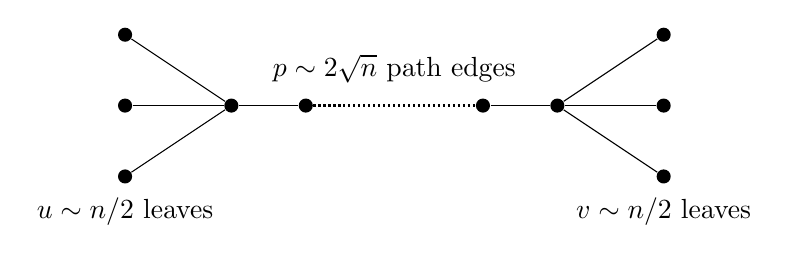
\begin{tikzpicture}[scale=.9,vertex/.style={circle,fill=black,inner sep=1.8pt}]
\node[vertex] (L) at (-2.3,0) {};
\node[vertex] (R) at (2.3,0) {};
\foreach \y in {-1,0,1} {
  \node[vertex] (a\y) at (-3.8,\y) {};
  \node[vertex] (b\y) at (3.8,\y) {};
  \draw (L)--(a\y); \draw (R)--(b\y);
}
\node[vertex] (A) at (-1.25,0) {};
\node[vertex] (B) at (1.25,0) {};
\draw (L)--(A); \draw[densely dotted,thick] (A)--(B); \draw (B)--(R);
\node at (0,.52) {$p\sim2\sqrt n$ path edges};
\node at (-3.8,-1.5) {$u\sim n/2$ leaves};
\node at (3.8,-1.5) {$v\sim n/2$ leaves};
\end{tikzpicture}
\caption{The balanced double-broom. Each fan denotes a larger family of
leaves. Leaf-edge cut counts are $n-1$, while central-path cut counts are
$n^2/4+O(n)$. Their proportions realize the extremal moment ratio.}
\label{p2:fig:double-broom}
\end{figure}

\subsection{A finite bound and its sharp asymptotic}

Define
\[
 M_n=\max\{\alpha(T):T\text{ is a tree on }n\text{ vertices}\},
 \quad
 a_n=\sqrt{n-1},
 \quad
 b_n=\sqrt{\lfloor n^2/4\rfloor}.
\]
The maximum exists because there are finitely many tree topologies on
$n$ vertices.

\begin{theorem}[Sharp tree approximation asymptotic]
\label{p2:thm:lewis-tree-sharp}
For every $n\geq2$ and every $n$-vertex tree $T$,
\begin{equation}\label{p2:eq:lewis-finite-upper}
 \alpha(T)\leq\frac{(a_n+b_n)^2}{4a_nb_n}.
\end{equation}
Moreover,
\begin{equation}\label{p2:eq:lewis-sharp-asymptotic}
 M_n=\frac{\sqrt n}{8}+\frac12+O(n^{-1/2})
 \qquad(n\longrightarrow\infty).
\end{equation}
Balanced double-brooms whose central paths have
$\lfloor2\sqrt n\rfloor$ edges attain the asymptotic in
\eqref{p2:eq:lewis-sharp-asymptotic}.
\end{theorem}

\begin{proof}
We first prove the upper bound.  Every tree edge satisfies
\[
 n-1\leq c_e\leq\lfloor n^2/4\rfloor.
\]
Put $x_e=\sqrt{c_e}$ and
$\mu=(n-1)^{-1}\sum_e x_e$.
The pointwise inequality $(x_e-a_n)(x_e-b_n)\leq0$ yields
\[
 \frac1{n-1}\sum_e x_e^2
 \leq(a_n+b_n)\mu-a_nb_n.
\]
By \eqref{p2:eq:lewis-tree-ratio},
\[
 \alpha(T)
 =\frac{(n-1)^{-1}\sum_e x_e^2}{\mu^2}
 \leq\frac{a_n+b_n}{\mu}-\frac{a_nb_n}{\mu^2}
 \leq\frac{(a_n+b_n)^2}{4a_nb_n}.
\]
For the last inequality one may maximize the scalar expression, whose
maximum occurs at $\mu=2a_nb_n/(a_n+b_n)$, or complete the square.
In particular,
\begin{equation}\label{p2:eq:lewis-upper-expansion}
 \frac{(a_n+b_n)^2}{4a_nb_n}
 =\frac{b_n}{4a_n}+\frac12+\frac{a_n}{4b_n}
 =\frac{\sqrt n}{8}+\frac12+O(n^{-1/2}).
\end{equation}

For the lower bound, fix $n\geq9$ and put
\[
 p=\lfloor2\sqrt n\rfloor,\qquad
 L=n-p-1,\qquad u=\lfloor L/2\rfloor,\qquad v=L-u.
\]
Take a path with $p$ edges, attach $u$ leaves to its left endpoint and
$v$ leaves to its right endpoint, and denote the resulting tree by
$T_n$.  It has exactly $n$ vertices and $n-1=L+p$ edges.
The $L$ leaf edges have cut count $n-1$.  For the $j$th path edge,
$1\leq j\leq p$, the cut count is
\begin{equation}\label{p2:eq:lewis-double-broom-cuts}
 c_j=(u+j)(n-u-j)=\frac{n^2}{4}-d_j^2,
 \qquad d_j=u+j-\frac n2.
\end{equation}
The choice of balanced leaf counts gives $|d_j|\leq p/2$.

Write $r=\sqrt n$ and $p=2r+t$, where $-1<t\leq0$.
Using $\sum_jd_j^2=O(p^3)$, we obtain
\begin{align}
 S_n:=\sum_{e\in E(T_n)}c_e
 &=L(n-1)+\frac{pn^2}{4}-\sum_{j=1}^{p}d_j^2\notag\\
 &=\frac{r^5}{2}+\left(\frac t4+1\right)r^4+O(r^3).
 \label{p2:eq:lewis-S-expansion}
\end{align}
For the square-root sum, the exact identity
\[
 0\leq\frac n2-\sqrt{\frac{n^2}{4}-d_j^2}
 =\frac{d_j^2}{n/2+\sqrt{n^2/4-d_j^2}}
 \leq\frac{2d_j^2}{n}
\]
shows that the total error on the path is $O(p^3/n)=O(r)$.
Since $\sqrt{n-1}=r-1/(2r)+O(r^{-3})$, it follows that
\begin{align}
 Q_n:=\sum_{e\in E(T_n)}\sqrt{c_e}
 &=L\sqrt{n-1}+\sum_{j=1}^{p}\sqrt{n^2/4-d_j^2}\notag\\
 &=2r^3+\left(\frac t2-2\right)r^2+O(r).
 \label{p2:eq:lewis-Q-expansion}
\end{align}
All remainder constants above are uniform in $t\in[-1,0]$ and in the
parity of $L$.
Substituting \eqref{p2:eq:lewis-S-expansion} and
\eqref{p2:eq:lewis-Q-expansion} into \eqref{p2:eq:lewis-tree-ratio} gives
\begin{align*}
 \alpha(T_n)
 &=\frac{(r^2-1)
       \{r^5/2+(t/4+1)r^4+O(r^3)\}}
       {4r^6+(2t-8)r^5+O(r^4)}\\
 &=\frac r8+\frac12+O(r^{-1}).
\end{align*}
The terms depending on $t$ cancel from the constant coefficient.
Together with \eqref{p2:eq:lewis-upper-expansion}, this proves
\eqref{p2:eq:lewis-sharp-asymptotic}.
\end{proof}

\begin{remark}[Why the extremal scale is a square root]
The ratio is the empirical second moment of the numbers
$\sqrt{c_e}$ divided by their squared empirical mean.
Leaf edges have $\sqrt{c_e}\simeq\sqrt n$, whereas the central edges of
a balanced double-broom have $\sqrt{c_e}\simeq n/2$.
About $2\sqrt n$ central edges balance these two contributions to the
first moment and asymptotically attain the interval moment bound.
Thus both the exponent and the leading constant arise from a genuine
extremal design calculation.
\end{remark}

\subsection{A rational certificate and the stated conjecture}

\begin{proposition}[An explicit finite counterexample]
\label{p2:prop:lewis-441}
Let $T$ consist of a path with $40$ edges, with $200$ new leaves
attached to each endpoint.  Then $T$ has $441$ vertices and
\[
 \alpha(T)>\frac{775676}{247107}>\frac{78}{25}=3.12.
\]
\end{proposition}

\begin{proof}
More generally, for an integer $k\geq1$, take a path with $4k$ edges
and attach $2k^2$ leaves to each endpoint.  Then $n=(2k+1)^2$ and
\[
 c_{\mathrm{leaf}}=n-1,
 \qquad
 c_j=(2k^2+j)(2k^2+4k+1-j),\quad 1\leq j\leq4k.
\]
Summation gives
\[
 S_k:=\sum_ec_e
 =\frac{4k}{3}(12k^4+36k^3+26k^2+6k+1).
\]
Since $\sqrt{n-1}<2k+1$ and $\sqrt{c_j}\leq n/2$,
\[
 Q_k:=\sum_e\sqrt{c_e}
 <4k^2(2k+1)+2kn
 =2k(2k+1)(4k+1).
\]
Therefore
\begin{equation}\label{p2:eq:lewis-rational-certificate}
 \alpha(T_k)>
 \frac{4(k+1)(12k^4+36k^3+26k^2+6k+1)}
      {3(2k+1)^2(4k+1)^2}.
\end{equation}
At $k=10$, the right-hand side is $775676/247107$, and
\[
 \frac{775676}{247107}-\frac{78}{25}
 =\frac{117554}{6177675}>0.
\]
Thus the certificate requires no floating-point approximation.
\end{proof}

\begin{corollary}[Negative resolution of the logarithmic comparison]
\label{p2:cor:lewis-conjecture-negative}
The $D$-optimal/infinity-Lewis effective-resistance approximation ratio
is not $O(\log n)$ on general graphs, or even on trees.
In particular, Conjecture~1.5 of
\cite{p2:SulimanWeinstein2023}, as stated in arXiv v1, is false.
The stronger Conjecture~4.6 in the same version is false as well.
\end{corollary}

\begin{proof}
Theorem~\ref{p2:thm:lewis-tree-sharp} supplies trees with
$\alpha(T_n)\sim\sqrt n/8$, and $\sqrt n/\log n\to\infty$.
The source's Theorem~1.4 bounds the actual approximation ratio above
by the quantity in its Conjecture~4.6, so that stronger proposed
logarithmic bound cannot hold either.
\end{proof}

\subsection{The subtree reduction does not preserve the ratio}

The discrepancy with the asserted constant tree bound can be traced
to a specific monotonicity step.  Claim~4.3 of
\cite{p2:SulimanWeinstein2023} asserts that $T\subset T'$ implies
$\alpha(T)\leq\alpha(T')$ for trees.  Under ordinary subtree
containment this assertion is false, as the following elementary
argument shows independently of the preceding asymptotic theorem.

\begin{proposition}[Failure of subtree monotonicity]
\label{p2:prop:lewis-nonmonotone}
There are trees $T\subset T'$ with $\alpha(T)>\alpha(T')$.
\end{proposition}

\begin{proof}
Take $T=P_4$, the path on four vertices.  Its cut counts are $3,4,3$;
hence
\[
 \alpha(P_4)=\frac{30}{(2\sqrt3+2)^2}>1.
\]
For $N\geq1$, attach $N$ new leaves to an endpoint of $P_4$, forming
$T_N\supset P_4$.  The new leaf edges have cut count $N+3$ and the
three original edges have cut counts
$3(N+1)$, $2(N+2)$, and $N+3$.  Thus
\[
 \sum_e c_e=N^2+9N+10,
\]
\[
 \sum_e\sqrt{c_e}
 =(N+1)\sqrt{N+3}+\sqrt{3(N+1)}+\sqrt{2(N+2)}
 =N^{3/2}+O(N^{1/2}).
\]
Since $|E(T_N)|=N+3$, formula \eqref{p2:eq:lewis-tree-ratio} gives
$\alpha(T_N)\to1$.  For all sufficiently large $N$,
$\alpha(T_N)<\alpha(P_4)$, proving the assertion.
\end{proof}

In the proposed monotonicity proof, a design on $T$ is treated as
feasible for the resistance problem on $T'$.  When vertices are
added, extending the old design by zero conductances disconnects
those new vertices and yields infinite total effective resistance;
it does not give the asserted comparison of optimal values.
The subsequent reduction from arbitrary bowties to a family with
three proportional size parameters therefore does not apply.
The extremal double-brooms above have a path of order $\sqrt n$ and
two leaf populations of order $n$, which is exactly the scale missed
by that reduction.


\section{Exact recurrence minimality for alternating binomial power sums}
\label{p2:sec:alternating}

For an integer $r\geq2$, consider McIntosh's alternating binomial sum
\begin{equation}\label{p2:eq:alt-definition}
 A_r(n)=\sum_{k=-n}^{n}(-1)^k\binom{2n}{n+k}^{r},\qquad n\geq0.
\end{equation}
McIntosh proved that this sequence has a polynomial-coefficient recurrence
with consecutive shift width at most $\lfloor r/2\rfloor$, and proved that
this width is minimal when $r$ is prime or a power of two
\cite[Theorems~1 and~2]{p3:McIntosh1993}. His lower-bound argument uses the
algebraic degree of the dominant exponential growth rate. That degree is
$\varphi(2r)/2$, which can be strictly smaller than $\lfloor r/2\rfloor$.
Here all the positive critical values of a real moment representation
provide the missing lower bounds.

By a recurrence we mean an eventual identity
\begin{equation}\label{p2:eq:alt-general-recurrence}
 \sum_{j\in J}q_j(n)A_r(n+j)=0,
 \qquad q_j\in\mathbb C(n)\setminus\{0\},
\end{equation}
where $J\subset\mathbb Z$ is finite and nonempty. Its \emph{shift width}
is $\max J-\min J$, and its \emph{number of terms} is $|J|$.
These are different quantities when the shifts have gaps.

\begin{theorem}\label{p2:thm:alt-minimality}
For every integer $r\geq2$, put $m=\lfloor r/2\rfloor$.
Every recurrence \eqref{p2:eq:alt-general-recurrence} has shift width at
least $m$ and at least $m+1$ nonzero terms. Both bounds are attained by
a recurrence with coefficients in $\mathbb Q[n]$.
Consequently the minimum shift width is $\lfloor r/2\rfloor$, and the
minimum number of terms, even allowing arbitrary gaps and coefficients
in $\mathbb C(n)$, is $\lfloor r/2\rfloor+1$.
\end{theorem}

The new assertion is the lower bound for every $r$, including the stronger
bound for sparse recurrences over $\mathbb C(n)$. Attainment uses the
general upper bound in McIntosh's Theorem~1. Thus the theorem removes the
prime-or-power-of-two restriction from his minimality conclusion; no
claim about an exhaustive historical priority search is needed for this
precise comparison.

\subsection{A positive moment representation}

Set $d=r-1$, $X=x_1\cdots x_d$, and
\begin{equation}\label{p2:eq:alt-laurent}
 P_r(x)=\prod_{i=1}^{d}(1+x_i)(1-X^{-1}).
\end{equation}
Here $\operatorname{CT}$ denotes the constant term in all $d$ variables.
For every integer $\ell\geq0$, direct expansion gives
\begin{equation}\label{p2:eq:alt-ct}
 \operatorname{CT}P_r^{\ell}
 =\sum_{j=0}^{\ell}(-1)^j\binom{\ell}{j}^{r}.
\end{equation}
Indeed, the term indexed by $j$ in the last factor forces the same
exponent $j$ in each of the other $d$ factors.

On $\mathbb T^d=(\mathbb R/2\pi\mathbb Z)^d$, write
$x_i=e^{i\theta_i}$ and $S=\sum_i\theta_i$. The elementary half-angle
identities yield
\begin{equation}\label{p2:eq:alt-real-function}
 P_r(e^{i\theta})=i\Psi_r(\theta),\qquad
 \Psi_r(\theta)=2^r\prod_{i=1}^{d}\cos(\theta_i/2)\sin(S/2).
\end{equation}
The half-angle expression is globally periodic: increasing one
$\theta_i$ by $2\pi$ changes both its cosine and the final sine by a
minus sign. Thus $\Psi_r=-iP_r|_{\mathbb T^d}$ is a globally real-analytic
real-valued function. Define
\begin{equation}\label{p2:eq:alt-positive-function}
 \Phi_r=\Psi_r^2=-P_r^2|_{\mathbb T^d}\geq0.
\end{equation}
For normalized Haar probability $\mu$ on the torus,
\begin{equation}\label{p2:eq:alt-positive-moment}
 A_r(n)=(-1)^n\operatorname{CT}P_r^{2n}
       =\int_{\mathbb T^d}\Phi_r(\theta)^n\,d\mu(\theta).
\end{equation}
The factor $(-1)^n$ comes from replacing $k$ by $j-n$ in
\eqref{p2:eq:alt-definition}. It is also exactly the factor contributed
by $P_r^{2n}=(-1)^n\Psi_r^{2n}$.

\subsection{The complete positive critical set}

\begin{lemma}\label{p2:lem:alt-critical-values}
The distinct positive critical values of $\Phi_r$ are
\begin{equation}\label{p2:eq:alt-values}
 v_j=\left(2\cos\frac{(2j+1)\pi}{2r}\right)^{2r},
 \qquad 0\leq j<m,\qquad m=\lfloor r/2\rfloor.
\end{equation}
Every critical point on each of these fibers is a nondegenerate local
maximum. There are no other critical points with $\Phi_r>0$.
\end{lemma}

\begin{proof}
At a point where $P_r\ne0$, all its factors are nonzero and
\begin{equation}\label{p2:eq:alt-critical-equations}
 x_i\frac{\partial}{\partial x_i}\log P_r
 =\frac{x_i}{1+x_i}+\frac1{X-1}.
\end{equation}
Its vanishing is equivalent to $x_iX=-1$. On the torus,
$\partial_{\theta_i}P_r=i x_i\partial_{x_i}P_r$; also $P_r=i\Psi_r$.
It follows that these equations are precisely the critical equations
for $\Psi_r$ away from its zero set. They force
$x_1=\cdots=x_d=\omega$ with $\omega^r=-1$. Conversely each such root
with $\omega\ne-1$ gives a critical point. The root $-1$ occurs only
for odd $r$ and has $P_r=0$, so it is excluded. Since
$d\Phi_r=2\Psi_r\,d\Psi_r$, this also exhausts the positive critical
set of $\Phi_r$.

At such a point $X=-1/\omega$, hence
$P_r=(1+\omega)^r$. With $\omega=e^{i(2j+1)\pi/r}$ this is
\[
 P_r=i(-1)^j
       \left(2\cos\frac{(2j+1)\pi}{2r}\right)^r.
\]
Conjugate roots produce equal values of $\Phi_r$. After pairing them,
the resulting values are exactly \eqref{p2:eq:alt-values}. Their angles
lie strictly between $0$ and $\pi/2$, so they are positive and strictly
decreasing. There are $m$ of them.

For the Hessian, let $I_d$ be the identity and $J_d$ the all-ones matrix.
Differentiating \eqref{p2:eq:alt-critical-equations} gives, at the critical
point,
\[
 \operatorname{Hess}_{\log x}\log P_r
 =\frac{\omega}{(1+\omega)^2}(I_d+J_d).
\]
The diagonal contribution is $\omega/(1+\omega)^2$. Every entry also
receives $-X/(X-1)^2$, which has the same value when $X=-1/\omega$.
If $\omega=e^{i\alpha}$, then
\[
 \frac{\omega}{(1+\omega)^2}
 =\frac1{4\cos^2(\alpha/2)}>0.
\]
Angular differentiation contributes a minus sign. On the real torus
one may use the real logarithm $\log|\Psi_r|$, whose Hessian agrees
with that of a local complex logarithm of $P_r$. Since the gradient
vanishes, this gives
\begin{equation}\label{p2:eq:alt-hessian}
 \operatorname{Hess}_{\theta}\Phi_r
 =-\frac{\Phi_r}{2\cos^2(\alpha/2)}(I_d+J_d).
\end{equation}
The eigenvalues of $I_d+J_d$ are $1$, with multiplicity $d-1$, and
$d+1=r$. The Hessian is therefore negative definite at every positive
critical point.
\end{proof}

\subsection{Visibility of every positive critical value}

We record the real-variable argument that prevents the smaller critical
values from disappearing under analytic continuation. In particular,
the argument includes the integer exponents that occur in even
dimensions.

\begin{lemma}\label{p2:lem:alt-visibility}
Let $M$ be a compact real-analytic manifold of dimension $d\geq1$, let
$\mu$ have a positive real-analytic density, and let $\Phi:M\to\mathbb R$
be real analytic. Suppose that the critical points in the fiber over
$v\ne0$ form a finite nonempty set and are all nondegenerate local
maxima. Regular points in that fiber are allowed. Then the generating
germ
\[
 F(t)=\int_M\frac{d\mu}{1-t\Phi}
\]
has a branch continued from $t=0$ that is singular at $t=1/v$.
\end{lemma}

\begin{proof}
The analytic Morse lemma gives local coordinates near each critical
point in which $\Phi=v-|y|^2$ and $d\mu=g(y)\,dy$, with $g$ analytic
and $g(0)>0$. For $w>0$ sufficiently small, the local density of
$\Phi_*\mu$ at $v-w$ is
\[
 \frac12w^{d/2-1}\int_{S^{d-1}}g(\sqrt w\,\omega)\,d\omega.
\]
The spherical average is analytic in $w$: odd Taylor terms integrate
to zero. Its constant term is positive. Choose smooth cutoffs equal
to one near the critical points. After restricting to a sufficiently
small interval about $v$, the remaining compact region contains only
regular points, so its pushforward has a smooth density. Summing the
critical contributions therefore gives
\begin{equation}\label{p2:eq:alt-density-defect}
 \frac{d\Phi_*\mu}{dx}(v+x)
 =b(x)+\mathbf 1_{\{x<0\}}(-x)^{d/2-1}h(-x),
\end{equation}
where $b$ is smooth, $h$ is analytic near zero, and $h(0)>0$.
There is no cancellation because all critical points contribute from
the same side with positive leading coefficients.

The density in \eqref{p2:eq:alt-density-defect} is not smooth at zero.
If $d$ is even, a finite derivative has a jump. If $d$ is odd and
$d\geq3$, a noninteger power prevents smoothness; for $d=1$, the
density is locally integrable but unbounded.

Consider the Cauchy transform
\[
 G(z)=\int_M\frac{d\mu}{z-\Phi}.
\]
It is holomorphic in the upper half-plane and satisfies
$G(z)=z^{-1}F(z^{-1})$ near infinity. Its boundary distribution is
\[
 -\frac1\pi\operatorname{Im}G(x+i0)=\Phi_*\mu,
\]
as follows from the Poisson kernel approximation to the identity.
If this upper-half-plane branch extended holomorphically through $v$,
its boundary imaginary part would be real analytic there. This
contradicts \eqref{p2:eq:alt-density-defect}. Thus the branch is singular
at $v$. The change of variables $t=1/z$, which is locally biholomorphic
at $v\ne0$, gives the claimed singularity at $1/v$. The continuation
from infinity in the upper half-plane corresponds to a continuation
of the generating germ from zero, including when $v$ is an interior
point of the real range of $\Phi$.
\end{proof}

Applying Lemmas~\ref{p2:lem:alt-critical-values} and
\ref{p2:lem:alt-visibility} to \eqref{p2:eq:alt-positive-moment} proves that
\begin{equation}\label{p2:eq:alt-generating-function}
 F_r(t)=\sum_{n\geq0}A_r(n)t^n
\end{equation}
has genuine continued-branch singularities at the $m$ distinct positive
points $t_j=1/v_j$. This assertion concerns all these continued
singularities, not merely the first singularity on the circle of
convergence.

\subsection{Singularities force width and support bounds}

\begin{lemma}\label{p2:lem:alt-sparse-budget}
Let $a_n$ have a generating function analytic near zero. Suppose its
continued germ has singularities at $m$ distinct positive finite
points. Then every eventual rational-coefficient recurrence for $a_n$
has shift width at least $m$ and at least $m+1$ nonzero terms, even if
its coefficients lie in $\mathbb C(n)$ and its shifts have gaps.
\end{lemma}

\begin{proof}
After translating the index, write the recurrence as
\[
 \sum_{j\in J}q_j(n)a_{n+j}=0,
 \qquad \min J=0,\qquad \max J=L.
\]
Clear denominators so that $q_j\in\mathbb C[n]$. Set
$e=\max_j\deg q_j$ and $c_j=[n^e]q_j$. Not all $c_j$ vanish.
Let $F(t)=\sum_{n\geq0}a_nt^n$ and $\vartheta=t\,d/dt$.
Multiplying by $t^{n+L}$ and summing over all sufficiently large $n$
gives
\begin{equation}\label{p2:eq:alt-recurrence-ode}
 \left(\sum_{j\in J}t^{L-j}q_j(\vartheta-j)\right)F(t)=R(t),
\end{equation}
where $R$ is a polynomial accounting for finitely many initial terms.
The coefficient of the highest ordinary derivative is $t^eH(t)$,
where
\begin{equation}\label{p2:eq:alt-leading-symbol}
 H(t)=\sum_{j\in J}c_jt^{L-j}\ne0.
\end{equation}
Distinct shifts give distinct monomials, so this leading coefficient
cannot vanish identically. Every nonzero finite singularity of a
continued solution of \eqref{p2:eq:alt-recurrence-ode} must be a zero of
$H$: otherwise the equation is an inhomogeneous linear differential
equation with an ordinary point and analytic right-hand side. For
$e=0$, the same conclusion follows directly from $H(t)F(t)=R(t)$.

Consequently $H$ has at least $m$ distinct positive roots. Since
$\deg H\leq L$, this implies $L\geq m$.
For the term bound, choose a nonzero real or imaginary part of $H$.
It is a real polynomial with the same $m$ positive roots and no more
nonzero monomials than $H$. Descartes' rule of signs implies that a
real polynomial with $k$ nonzero monomials has at most $k-1$ positive
roots. Thus $H$ has at least $m+1$ nonzero monomials. Formula
\eqref{p2:eq:alt-leading-symbol} now gives $|J|\geq m+1$.
\end{proof}

\begin{proof}[Proof of Theorem~\ref{p2:thm:alt-minimality}]
The moment representation and the complete critical-point calculation
give $m$ distinct positive singularities of $F_r$ by
Lemma~\ref{p2:lem:alt-visibility}. Lemma~\ref{p2:lem:alt-sparse-budget}
proves both lower bounds over $\mathbb C(n)$. McIntosh's general
existence theorem supplies a recurrence over $\mathbb Q[n]$ with shifts
in an interval of length $m$ \cite[Theorem~1]{p3:McIntosh1993}. It has at
most $m+1$ positions; the lower bounds force it to attain both claimed
minima.
\end{proof}

\begin{corollary}\label{p2:cor:alt-symbol}
For any minimum-width recurrence, translate the shifts to
$0,\ldots,m$ and define its highest-degree symbol $H$ by
\eqref{p2:eq:alt-leading-symbol}. Then
\begin{equation}\label{p2:eq:alt-exact-symbol}
 H(t)=c\prod_{j=0}^{m-1}(1-v_jt),\qquad c\ne0.
\end{equation}
The set of nonzero finite points at which some branch of $F_r$
continued from zero is singular is exactly $\{1/v_j:0\leq j<m\}$.
\end{corollary}

\begin{proof}
The polynomial $H$ has degree at most $m$ and already has the $m$
distinct roots $1/v_j$, so \eqref{p2:eq:alt-exact-symbol} follows.
The differential equation \eqref{p2:eq:alt-recurrence-ode} has no other
nonzero finite nonordinary points, hence no continued solution branch
can acquire a singularity elsewhere. Visibility supplies a singular
branch at every displayed point.
\end{proof}

\subsection{The first missing composite case}

For $r=6$, the three critical scales are
\[
 v_0=1351+780\sqrt3,\qquad v_1=64,\qquad
 v_2=1351-780\sqrt3.
\]
The dominant scale has algebraic degree two, so the dominant-growth
argument alone cannot prove the correct width three. The rational
interior scale $64$ supplies the third visible singularity. Theorem
\ref{p2:thm:alt-minimality} gives width three and at least four nonzero
terms for every sparse recurrence. Moreover,
\[
 \prod_{j=0}^{2}(X-v_j)
 =(X-64)(X^2-2702X+1)
 =X^3-2766X^2+172929X-64.
\]
Thus a minimum-width recurrence has highest-degree generating symbol
proportional to
\[
 1-2766t+172929t^2-64t^3.
\]
For comparison, $r=2$ and $r=3$ have the sole critical scales $4$ and
$27$, respectively, in agreement with the familiar hypergeometric
formulas $A_2(n)=\binom{2n}{n}$ and $A_3(n)=(3n)!/(n!)^3$.


% Section fragment. Uses amsmath, amssymb, amsthm and hyperref.
% Environments theorem, lemma, proposition, remark, proof are assumed.
\section{Nonresonant connection coefficients for Jacobi trace densities}
\label{p2:sec:jacobi-connection}

\subsection{The published connection problem and the new scope}

Forrester and Kumar explicitly identify the determination of the scalars
in the Frobenius representation of the Jacobi trace density as the
connection problem left by Davis.  Their Proposition 1.3 and equation
(3.55) solve that problem when the endpoint parameter $b$ and the Dyson
index $\beta$ are nonnegative integers.  Their discussion after equation
(3.54) states that the general problem remains; see
\emph{Differential recurrences for the distribution of the trace of the
$\beta$-Jacobi ensemble}, Physica D \textbf{434} (2022), 133220,
\texttt{arXiv:2011.00787v2}, Section 3.3 \cite{p8:SFB_FK}.

Here the corner Fourier amplitudes determine those physical-density
connection scalars for real, noninteger parameters, provided the local
exponents are nonintegral.  The answer uses an explicitly specified upper
half-plane continuation.  It generalizes the sign in the integer-parameter
formula to a complex phase.  The theorem concerns the particular physical
density, not the full connection matrix between arbitrary bases.  Resonant
exponents and numerical stability of long continuation chains are not
settled by it.

Fix
\begin{equation}\label{p2:eq:JC-parameters}
 N\ge1,\qquad a>-1,\qquad b>0,\qquad \beta\ge0.
\end{equation}
The stronger restriction $b>0$ makes every component of the published
auxiliary integral system absolutely integrable.  Define
\[
 S_N(a,b,\beta)=\int_{[0,1]^N}|\Delta(u)|^\beta
                    \prod_{i=1}^N u_i^a(1-u_i)^b\,du
\]
and let $\rho(t)$ be the density of $\sum_{i=1}^N u_i$ under this
normalized measure, extended by zero outside $[0,N]$.
For $r\ge0$ put
\begin{align*}
 W_r(q,\beta)
 &=\int_{(0,\infty)^r}e^{-\sum x_i}|\Delta(x)|^\beta
                                  \prod x_i^q\,dx,\qquad W_0=1,\\
 &=\prod_{j=0}^{r-1}
   \frac{\Gamma(q+1+j\beta/2)\Gamma(1+(j+1)\beta/2)}
        {\Gamma(1+\beta/2)}.
\end{align*}
Only $q=a,b>-1$ will occur.  The Laguerre--Selberg and Selberg
evaluations give this product and
\[
 S_N(a,b,\beta)=\prod_{j=0}^{N-1}
 \frac{\Gamma(a+1+j\beta/2)\Gamma(b+1+j\beta/2)
              \Gamma(1+(j+1)\beta/2)}
 {\Gamma(a+b+2+(N+j-1)\beta/2)\Gamma(1+\beta/2)}.
\]

For $0\le p\le N$ define
\begin{align}
 \alpha_p&=(N-p)(a+1)+\frac\beta2(N-p)(N-p-1),\notag\\
 \eta_p&=p(b+1)+\frac\beta2p(p-1),\notag\\
 D_p&=\alpha_p+\eta_p,\qquad \gamma_p=D_p-1,\label{p2:eq:JC-exponents}\\
 K_p&=\binom Np\frac{W_{N-p}(a,\beta)W_p(b,\beta)}{S_N(a,b,\beta)}.
 \label{p2:eq:JC-K}
\end{align}
Here $D_p>0$ and $K_p>0$.  Our nonresonance assumption is
\begin{equation}\label{p2:eq:JC-nonresonance}
 \gamma_p\notin\mathbb Z\qquad(0\le p<N).
\end{equation}
It removes a countable collection of parameter hyperplanes; it does not
require $a,b$ or $\beta$ to be rational.  The exponent at the final
endpoint $p=N$ need not be nonintegral, since no continuation across
that endpoint is needed to represent the density on $(0,N)$.

\subsection{The normalized Frobenius branches}

We specify the branches through the Forrester--Kumar system, so that the
normalization of the coefficients below is unambiguous.  With indices
$j=0,\ldots,N$, set
\[
 \Lambda=-\operatorname{diag}(N,N-1,\ldots,0),\qquad
 h=a+b+1+\tfrac\beta2(2N-1),\qquad k=b+\tfrac\beta2N,
\]
and let $X$ be tridiagonal, with entries
\begin{align*}
 X_{j,j-1}&=u_j=-jk+\tfrac\beta2j^2,\\
 X_{j,j}&=v_j=hj-\tfrac\beta2(N-j)(2j+1)+k(N-2j)-1,\\
 X_{j,j+1}&=w_j=h(j-N)+\tfrac\beta2(N-j)(N-j-1)+k(N-j).
\end{align*}
Entries outside the index range are omitted.  The published system is
\begin{equation}\label{p2:eq:JC-system}
 (tI+\Lambda)G'(t)=XG(t).
\end{equation}
To relate it to the physical density, form
\[
 H_j(t)=\binom Nj^{-1}\int_{[0,1]^N}
 \delta\Bigl(t-\sum u_i\Bigr)|\Delta(u)|^\beta
 \prod u_i^a(1-u_i)^{b-1}e_j(1-u_1,\ldots,1-u_N)\,du.
\]
If $P_{jk}=\binom{N-j}{N-k}$, then $G=P^{-1}H$ satisfies
\eqref{p2:eq:JC-system}.  The last row of $P$ is the last coordinate row,
so
\begin{equation}\label{p2:eq:JC-physical-component}
 G_N(t)=H_N(t)=S_N(a,b,\beta)\rho(t).
\end{equation}
These are Proposition 3.9 and equation (3.48) of the cited paper.
They also hold at $\beta=0$, by the same integration identities or
by continuity.  On every interval between the integers the system is
ordinary, so its distributional solution is real analytic there.

\begin{lemma}[A uniquely normalized singular branch]
\label{p2:lem:JC-Frobenius}
Fix $p\in\{0,\ldots,N\}$ with $\gamma_p\notin\mathbb Z$.
At $t=p$, the system \eqref{p2:eq:JC-system} has $N$ holomorphic local
solutions and one nonintegral Frobenius solution.  The last component
of the latter, after a unique constant normalization, has the form
\begin{equation}\label{p2:eq:JC-Fp}
 F_p(t)=(t-p)^{\gamma_p}U_p(t-p),\qquad U_p(0)=1,
\end{equation}
where $U_p$ is holomorphic with real Taylor coefficients.  Initially
$t-p>0$ and the power is positive real.  Any last component of a local
solution is the sum of a holomorphic function and a constant multiple
of this Frobenius branch, with the branch of the power specified.
\end{lemma}

\begin{proof}
Put $j_0=N-p$ and $s=t-p$.  The residue matrix is the matrix with
only row $j_0$ nonzero, that row being row $j_0$ of $X$.  It has
rank one, with its nonzero eigenvalue
\[
 v_{j_0}=\gamma_p-p=:v.
\]
This identity follows by substitution into the displayed definition
of $v_j$.  The hypothesis $\gamma_p\notin\mathbb Z$ implies that
$v$ is nonintegral, so the residue is diagonalizable with eigenvalues
$0$ and $v$, and no difference between them is a nonzero integer.
The ordinary nonresonant Frobenius construction gives $N$ holomorphic
solutions and one solution
\[
 s^v\sum_{\ell\ge0}g_\ell s^\ell,\qquad g_0=e_{j_0}.
\]
For completeness, substitution gives the recurrence
\[
 (v+\ell)(pI+\Lambda)g_\ell
       =(X-(v+\ell-1)I)g_{\ell-1}.
\]
Tridiagonality shows that its last component vanishes up to
$\ell=p-1$, while
\begin{equation}\label{p2:eq:JC-normalization}
 (g_p)_N=
 \frac{\prod_{\ell=1}^{p}u_{N-p+\ell}}
 {p!\prod_{\ell=1}^{p}(v+\ell)}\ne0.
\end{equation}
Indeed, the first contribution to row $N-p+\ell$ travels through
its subdiagonal entry $u_{N-p+\ell}$, and that row of
$pI+\Lambda$ has diagonal entry $\ell$.  Each numerator is
$-j(b+\beta(N-j)/2)$ with $j\ge1$, hence is nonzero by $b>0$;
the denominators are nonzero by nonresonance.  For $p=0$, the
empty product is one.  Division by \eqref{p2:eq:JC-normalization}
gives \eqref{p2:eq:JC-Fp}, since $v+p=\gamma_p$.  The nonintegral
Frobenius line is unique, and all coefficients are real.
\end{proof}

Write $F_p^{\uparrow}(t)$ for its continuation from just to the right
of $p$ to a real $t>p$, moving to the right and passing every intervening
integer by a small semicircle in the \emph{upper} half-plane.  This
fixes a homotopy class and hence a branch.  In particular, when a germ
on the left of a knot is continued to its right in this convention,
$(-s)^\gamma$ becomes $e^{-\pi i\gamma}s^\gamma$.

\subsection{The connection formula}

\begin{theorem}[Physical-density connection coefficients]
\label{p2:thm:JC-connection}
Assume \eqref{p2:eq:JC-parameters} and \eqref{p2:eq:JC-nonresonance}.
For $0\le p<N$ set
\begin{equation}\label{p2:eq:JC-Cp}
 \boxed{\displaystyle
 C_p=e^{-\pi i\eta_p}\frac{K_p}{\Gamma(D_p)}
 =e^{-\pi i\eta_p}\binom Np
 \frac{W_{N-p}(a,\beta)W_p(b,\beta)}
      {S_N(a,b,\beta)\Gamma(D_p)}.}
\end{equation}
For each $p\in\{0,\ldots,N-1\}$, let
$\rho_{p,-}^{\uparrow}$ be the continuation to the right of
$p$ of the density germ on its left, with the upper convention.
Let $\rho_{p,+}$ be its physical germ on the right.  At $p=0$
use the zero density on the exterior left interval.  Then
\begin{equation}\label{p2:eq:JC-local-jump}
 \rho_{p,+}(t)-\rho_{p,-}^{\uparrow}(t)=C_pF_p(t)
 \qquad(t>p\text{ sufficiently close to }p).
\end{equation}
Consequently, for $k=0,\ldots,N-1$ and $k<t<k+1$,
\begin{equation}\label{p2:eq:JC-global}
 \boxed{\displaystyle
 \rho(t)=\sum_{p=0}^{k}C_pF_p^{\uparrow}(t).}
\end{equation}
Although the summands can be complex, their sum is the real, positive
physical density.  The lower-half-plane formula is its complex conjugate.
If in addition $\gamma_N\notin\mathbb Z$, the local jump
\eqref{p2:eq:JC-local-jump} also holds at $p=N$, with the same formula
\eqref{p2:eq:JC-Cp} and zero physical density on the right.
\end{theorem}

The distinction between \eqref{p2:eq:JC-local-jump} and a one-sided real
coefficient is essential.  At noninteger parameters the density generally
has nonanalytic terms on \emph{both} sides of an interior knot.  The
coefficient $C_p$ is the discrepancy after a specified analytic
continuation; it is not, in general, the coefficient on the right alone.

\begin{lemma}[The complete local Fourier symbol]
\label{p2:lem:JC-symbol}
Fix $p\in\{0,\ldots,N\}$.  Let $\chi$ be smooth, supported in a
sufficiently small interval about $p$, and identically one near $p$.  Then as $R\to+\infty$,
\begin{equation}\label{p2:eq:JC-local-Fourier}
 \int e^{iRt}\chi(t)\rho(t)\,dt
 \sim e^{ipR}R^{-D_p}\sum_{\ell\ge0}A_{p,\ell}R^{-\ell},
 \qquad
 A_{p,0}=K_p e^{\frac{\pi i}{2}(\alpha_p-\eta_p)}.
\end{equation}
The expansion is complete to every prescribed finite order.
If $D_p$ is nonintegral, there are no additional integer-power terms
at this frequency.
\end{lemma}

\begin{proof}
Insert the defining pushforward integral for $\rho$.  The relevant
corners of the cube have $p$ coordinates equal to one and $N-p$
equal to zero.  Near one of these corners use $x_i=u_i$ in the
zero cluster and $y_i=1-u_i$ in the one cluster.  The phase becomes
$p+\sum x_i-\sum y_i$.  The weight is
\[
 |\Delta(x)|^\beta\prod x_i^a\;
 |\Delta(y)|^\beta\prod y_i^b\;B(x,y),
 \qquad B(0,0)=1,
\]
where $B$ is analytic near the origin.  The two homogeneous weights,
including their measures, have degrees $\alpha_p$ and $\eta_p$.
Radial integration with $r=\sum x_i$ and $q=\sum y_i$ reduces their
leading Fourier integrals to the one-dimensional endpoint formula
\[
 \int_0^\infty e^{\pm iRr}r^{d-1}\chi_0(r)\,dr
     \sim \Gamma(d)e^{\pm\pi i d/2}R^{-d},
 \quad d>0,
\]
where $\chi_0$ is smooth and equals one near zero.  For nonempty clusters the angular constants are
$W_{N-p}(a,\beta)/\Gamma(\alpha_p)$ and
$W_p(b,\beta)/\Gamma(\eta_p)$, respectively; an empty cluster
contributes one without radial integration.  The angular integrals
are over compact simplexes with integrable weights.  Consequently,
after choosing smooth cutoffs in $r$ and $q$, angular integration
of $B$ produces a smooth amplitude in these two radial variables,
with Taylor remainders of every order.  Applying the endpoint
formula successively in $r$ and $q$ gives a complete expansion.
Taylor expansion of $B$ gives only integer increments of $D_p$.
Thus one corner contributes the claimed leading coefficient without
the binomial factor, and all $\binom Np$ corners contribute identically.

To justify the complete expansion and exclude other contributions,
cover the complement of the corner neighbourhoods by small sets.
At every point of this complement, some cluster of coincident
coordinates lies strictly between zero and one.  Translating all
coordinates of that cluster together leaves its internal differences
unchanged, is tangent to all relevant collision faces, and has
nonzero phase derivative equal to the cluster size.  Other factors
in the translated coordinates are smooth and nonzero.  A smooth
partition of unity and repeated integration by parts in this
direction give an error $O(R^{-M})$ for every $M$, even when
$\beta$ is not integral.  Differentiated factors are bounded by
integrable endpoint and collision weights.  The radial endpoint
expansions of the corner pieces have remainders to arbitrary order.
This proves the complete expansion and the absence of another power
scale in \eqref{p2:eq:JC-local-Fourier}.
\end{proof}

\begin{proof}[Proof of Theorem~\ref{p2:thm:JC-connection}]
Fix a knot $p$ with $\gamma_p\notin\mathbb Z$, and abbreviate
$D=D_p$, $\gamma=\gamma_p$, $\alpha=\alpha_p$,
$\eta=\eta_p$, and $K=K_p$.  By
Lemma~\ref{p2:lem:JC-Frobenius}, on the two real sides of $s=t-p=0$
the physical density has the form
\begin{equation}\label{p2:eq:JC-two-sides}
 \rho(p+s)=
 \begin{cases}
  a_+(s)+c_+s^\gamma U_p(s),&s>0,\\
  a_-(s)+c_-(-s)^\gamma U_p(s),&s<0,
 \end{cases}
\end{equation}
where $a_\pm$ are holomorphic near zero and $c_\pm$ are real.
At an endpoint the exterior expression is zero.  The reality follows
from the real equation and the real normalization of $U_p$.

We first prove $a_+=a_-$.  After multiplication by a cutoff, a
nonzero first Taylor coefficient of $a_+-a_-$ of degree $q$ would
give a nonzero term of order $R^{-q-1}$ in the Fourier transform
at frequency $p$.  In contrast, the nonanalytic terms in
\eqref{p2:eq:JC-two-sides} give only powers $R^{-D-\ell}$,
$\ell\ge0$.  Since $D$ is nonintegral, the two power scales are
disjoint.  Lemma~\ref{p2:lem:JC-symbol} supplies a complete expansion
containing only the second scale.  Uniqueness of an asymptotic power
expansion forces every Taylor coefficient of $a_+-a_-$ to vanish.
The two holomorphic functions are therefore identical.  This step
is why leading asymptotics alone would not suffice for the proof.

Comparing the leading Fourier coefficient in
\eqref{p2:eq:JC-two-sides} with \eqref{p2:eq:JC-local-Fourier} gives
\[
 \Gamma(D)\left(c_+e^{\pi iD/2}+c_-e^{-\pi iD/2}\right)
       =K e^{\pi i(\alpha-\eta)/2}.
\]
The real and imaginary parts uniquely determine the two real
coefficients because $\sin(\pi D)\ne0$.  They are
\begin{equation}\label{p2:eq:JC-one-sided}
 c_+=\frac{K\sin(\pi\alpha)}{\Gamma(D)\sin(\pi D)},
 \qquad
 c_-=\frac{K\sin(\pi\eta)}{\Gamma(D)\sin(\pi D)}.
\end{equation}
These formulas remain meaningful when an individual sine in the
numerator vanishes.  They also cover the empty-cluster endpoints.

Under upper-half-plane continuation of the left germ,
$(-s)^\gamma$ becomes $e^{-\pi i\gamma}s^\gamma$.
As the analytic backgrounds agree, the discrepancy is
\[
 (c_+-e^{-\pi i\gamma}c_-)F_p(t).
\]
Using $D=\alpha+\eta$ and $\gamma=D-1$,
\[
 \sin(\pi\alpha)-e^{-\pi i\gamma}\sin(\pi\eta)
    =e^{-\pi i\eta}\sin(\pi D).
\]
Substitution into \eqref{p2:eq:JC-one-sided} gives exactly
$C_p=K e^{-\pi i\eta}/\Gamma(D)$ and proves
\eqref{p2:eq:JC-local-jump}.

At $p=0$ the density on the left is zero, so the first interval
satisfies $\rho=C_0F_0$.  Continue this identity to the next knot
through the specified upper path and add the local discrepancy
$C_1F_1$.  The identity extends throughout the next interval by
analytic continuation of the same differential system.  Inductively,
this proves \eqref{p2:eq:JC-global}.  Reversing upper and lower paths
conjugates the coefficients and branches.
\end{proof}

\subsection{Comparison, checks, and limitations}

When $b$ is a positive integer and $\beta$ is a nonnegative integer,
\[
 \eta_p=p(b+1)+\frac\beta2p(p-1)\in\mathbb Z,
 \qquad e^{-\pi i\eta_p}=(-1)^{p(b+1)+\beta p(p-1)/2}.
\]
If $a$ is irrational, all exponents $\gamma_p$ with $p<N$ are
nonintegral.  Thus the theorem has a nonempty intersection with the
integer-parameter result, and \eqref{p2:eq:JC-Cp} there is exactly the
sign and Laguerre--Selberg constant of Forrester--Kumar (1.12),
Proposition 3.4, and (3.55).  Their $b=0$ boundary case is not included
in the present auxiliary-integral hypothesis.
The new range is the nonresonant real-parameter range outside those
integer restrictions.  In that range the coefficient on the left of
an interior knot generally does not vanish, and the continuation
convention is indispensable.

As an exact consistency test of the additional final-endpoint
statement, take $N=1$ and $a,b\notin\mathbb Z$.  The density is
$t^a(1-t)^b/B(a+1,b+1)$ on $(0,1)$.  At $t=1$ its upper
continuation is $e^{-\pi ib}(t-1)^b t^a/B(a+1,b+1)$.
Formula \eqref{p2:eq:JC-Cp} gives
$C_1=e^{-\pi i(b+1)}/B(a+1,b+1)$, precisely the coefficient
that cancels this branch to produce the zero exterior density.

A second, noninteger numerical diagnostic uses the exact $N=2$
hypergeometric density in Forrester--Kumar (3.36)--(3.37).
For $a=0.2$, $b=0.35$, $\beta=0.7$, the predicted coefficient at
$p=1$ is
\[
 C_1=-3.7279987849354161471+7.3166095798246842339\,i.
\]
Evaluating the difference between the physical right density and the
upper continuation of the left density, then dividing by
$(t-1)^{a+b+1}$, converges to this value as $t\downarrow1$.
This diagnostic does not replace the proof.

\begin{remark}[Remaining questions]
This result does not assert a full connection matrix for arbitrary
Frobenius bases, a uniform error bound for numerical continuation,
or a treatment of resonant $\gamma_p\in\mathbb Z$.  Resonance can
introduce logarithms and requires a separately normalized limiting
basis; simply substituting resonant parameters into
\eqref{p2:eq:JC-one-sided} would be invalid.  The condition $b>0$
has also been retained instead of asserting an unproved extension
through divergent auxiliary integrals.  A broader priority audit
of general Selberg connection formulas remains necessary before
any claim of historical first solution.
\end{remark}


% Section fragment.  Required packages: amsmath, amssymb, amsthm, hyperref.
% Bibliography entry for the parent document:
% \bibitem{abraham2025frontiers} K. Abraham, E. Gassiat and Z. Naulet,
% Frontiers to the learning of nonparametric hidden Markov models,
% Journal of Machine Learning Research 26(155) (2025), 1--75.
% https://jmlr.org/papers/v26/24-2230.html

\section{One hidden-refresh trajectory: sharp costs at both persistence boundaries}
\label{p2:sec:long-chain}

A population that is invisible from one observation can become identifiable
through temporal dependence.  For a fixed known emission family, the preceding
three-visit construction gives a persistence-dependent rate from independent
triples.  This section removes that independence assumption: all observations
now come from one stationary trajectory.  Two distinct obstructions must be
controlled simultaneously.  As persistence tends to zero, the one-view defect
reappears.  As persistence tends to one, the trajectory contains too few fresh
population draws.  We obtain matching upper and lower bounds over an interval
containing both boundaries, using an estimator that knows neither boundary
margin.  The proof of the small-persistence lower bound compares full-history
filters; a calculation for isolated triples alone would not suffice.

\subsection{A fixed analytic emission family and the statistical experiment}

Let $U$ be uniform probability on $[0,1]$, and write
$L_j(x)=P_j(2x-1)$ for the shifted Legendre polynomial of degree $j$.
Set
\begin{equation}\label{p2:eq:lc-kernel}
 v_j(\theta)=\theta^j-\frac{2\theta}{j+1},\qquad
 k(x\mid\theta)=1+\sum_{j=2}^{\infty}
                  \frac{L_j(x)v_j(\theta)}{8j!},
 \quad x,\theta\in[0,1].
\end{equation}
The family $k$ is known.  Factorial decay makes the series normally convergent
on every compact subset of $\mathbb C^2$, so it defines an entire function.
The identities $\int L_j\,dU=0$ and $\int v_j\,dU=0$ show that
\begin{equation}\label{p2:eq:lc-cancellation}
 \int k(x\mid\theta)\,dU(x)=1,
 \qquad k(x\mid0)=1,
 \qquad \int k(x\mid\theta)\,dU(\theta)=1.
\end{equation}
Since $|L_j|\le1$ and $|v_j|\le2$ on the real unit interval,
\begin{equation}\label{p2:eq:lc-bounds}
 |k-1|\le\frac{e-2}{4}<\frac14,
 \qquad \frac34\le k\le\frac54.
\end{equation}
In particular $k(\cdot\mid\theta)$ is a strictly positive probability density.

For $s\in[1/2,1]$ let
\begin{equation}\label{p2:eq:lc-population}
 G_s=(1-s)\delta_0+sU.
\end{equation}
The latent chain is stationary with population $G_s$ and transition kernel
\begin{equation}\label{p2:eq:lc-transition}
 M_{s,\rho}(\theta,d\eta)
   =\rho\delta_\theta(d\eta)+(1-\rho)G_s(d\eta),
 \qquad 0<\rho<1.
\end{equation}
Conditionally on the latent path, observations are independent with density
$k(\cdot\mid\theta_i)$.  Both $s$ and $\rho$ are unknown.  The data consist of
\emph{one complete trajectory} $(X_1,\ldots,X_n)$; denote its law by
$\mathsf P^{(n)}_{s,\rho}$.  By \eqref{p2:eq:lc-cancellation}, every individual
observation has law $U$, independently of $s$ and $\rho$.

We estimate the population in Wasserstein distance $W_1$ for the usual metric
on $[0,1]$.  The one-dimensional distribution-function formula gives
\begin{equation}\label{p2:eq:lc-wasserstein}
 W_1(G_s,G_t)=\frac{|s-t|}{2}.
\end{equation}
The infima below allow arbitrary measurable probability-valued estimators,
not just estimates within the family \eqref{p2:eq:lc-population}.

\begin{theorem}[Two-boundary minimax rate from one path]
\label{p2:thm:lc-main}
For $0<r\le1/8$, $0<q\le1/4$ and $n\ge1$, define
\[
 R_n(r,q)=\inf_{\widehat G}\ 
 \sup_{\substack{s\in[1/2,1]\\\rho\in[r,1-q]}}
 \mathbb E_{s,\rho}W_1(\widehat G,G_s).
\]
There are constants $0<c<C<\infty$, depending only on the fixed emission
family, such that
\begin{equation}\label{p2:eq:lc-main-rate}
 c\min\left\{1,\frac{r^{-2}+q^{-1/2}}{\sqrt n}\right\}
 \le R_n(r,q)\le
 C\min\left\{1,\frac{r^{-2}+q^{-1/2}}{\sqrt n}\right\}.
\end{equation}
A single estimator $\widehat G_n$, using neither $r$ nor $q$, satisfies the
stronger pointwise upper bound
\begin{equation}\label{p2:eq:lc-pointwise}
 \mathbb E_{s,\rho}W_1(\widehat G_n,G_s)
 \le C\min\left\{1,\frac1{\sqrt n\,\rho^2\sqrt{1-\rho}}\right\},
 \qquad s\in[1/2,1],\quad 0<\rho<1.
\end{equation}
\end{theorem}

The rate in \eqref{p2:eq:lc-main-rate} contains the sum, equivalently the maximum,
of two boundary costs.  A product $r^{-2}q^{-1/2}$ would lose this information:
one value of $\rho$ cannot lie close to both zero and one.  The restrictions on
$r,q$ guarantee that both lower-bound experiments lie in the parameter
interval; the upper bound applies throughout that interval, including its
interior.

\begin{corollary}[Exact uniform-consistency criterion]
\label{p2:cor:lc-consistency}
For sequences $r_n\in(0,1/8]$ and $q_n\in(0,1/4]$, uniform consistent
population estimation over the corresponding classes is possible if and only if
\[
 nr_n^4\longrightarrow\infty
 \qquad\hbox{and}\qquad nq_n\longrightarrow\infty.
\]
\end{corollary}
\begin{proof}
Apply both sides of \eqref{p2:eq:lc-main-rate}.  A sum of two nonnegative
sequences tends to zero exactly when both summands do.
\end{proof}

\subsection{An estimator that needs neither persistence margin}

Let $\phi=80L_2$ and $a=2/135$.  Legendre orthogonality gives
\[
 \int \phi(x)k(x\mid\theta)\,dU(x)=v_2(\theta),
 \qquad \int v_2(\theta)^2\,dU(\theta)
 =\frac15-\frac13+\frac4{27}=a.
\]
Also $v_2(0)=0$ and $\int v_2\,dU=0$.  The refresh transition has powers
$M_{s,\rho}^h=\rho^h I+(1-\rho^h)G_s$.  Conditional independence of
emissions therefore yields, for every integer $h\ge1$,
\begin{equation}\label{p2:eq:lc-moments}
 \mathbb E_{s,\rho}
    \frac{\phi(X_i)\phi(X_{i+h})}{a}=s\rho^h.
\end{equation}

For $n\ge4$, put $m=n-2$ and define the overlapping-window averages
\[
 \widehat V=\frac1m\sum_{i=1}^{m}
                  \frac{\phi(X_i)\phi(X_{i+1})}{a},\qquad
 \widehat W=\frac1m\sum_{i=1}^{m}
                  \frac{\phi(X_i)\phi(X_{i+2})}{a}.
\]
Their mean vector is $(v,w)=(s\rho,s\rho^2)$.

\begin{lemma}[Variance of overlapping windows]\label{p2:lem:lc-variance}
There is a fixed constant $C$ such that
\begin{equation}\label{p2:eq:lc-variance}
 \mathbb E_{s,\rho}
       \bigl[(\widehat V-v)^2+(\widehat W-w)^2\bigr]
 \le\frac C{n(1-\rho)}.
\end{equation}
\end{lemma}
\begin{proof}
Each summand is a bounded function of the block $(X_i,X_{i+1},X_{i+2})$.
For two such blocks with starting positions separated by $\ell\ge3$,
condition on the latent state at the right endpoint of the first block and
the state at the left endpoint of the second.  Across the intervening gap,
the transition is
\[
 M_{s,\rho}^{\ell-2}
   =\rho^{\ell-2}I+(1-\rho^{\ell-2})G_s.
\]
The second term produces the product of the two expectations.  It follows
that the absolute covariance is at most $C\rho^{\ell-2}$.  Overlaps with
$\ell\le2$ have covariance at most $C$.  Summing the covariance series,
and using $m\ge n/2$, proves \eqref{p2:eq:lc-variance}.
\end{proof}

Choose a measurable minimizer $(\widehat s,\widehat\rho)$ of
\begin{equation}\label{p2:eq:lc-projection}
 (\widehat V-s'\rho')^2+(\widehat W-s'\rho'^2)^2
 \quad\hbox{over}\quad
 (s',\rho')\in[1/2,1]\times[0,1].
\end{equation}
Existence follows from compactness and continuity; a fixed measurable
tie-breaking rule supplies measurability.  Set $\widehat G_n=G_{\widehat s}$.
For $n<4$, use a fixed member of the population family.

\begin{lemma}[A global inverse with the true persistence in its denominator]
\label{p2:lem:lc-inverse}
Let $s,s'\in[1/2,1]$, $0<\rho\le1$, $0\le\rho'\le1$, and put
$(v,w)=(s\rho,s\rho^2)$ and $(v',w')=(s'\rho',s'\rho'^2)$.  Then
\begin{equation}\label{p2:eq:lc-inverse}
 |s-s'|\le\frac4{\rho^2}
                 \bigl(|v-v'|+|w-w'|\bigr).
\end{equation}
The candidate persistence $\rho'$ may be zero.
\end{lemma}
\begin{proof}
The polynomial identities $v^2=sw$ and $v'^2=s'w'$ hold even at $\rho'=0$.
Consequently
\[
 w(s-s')=v^2-v'^2+s'(w'-w).
\]
Since $w\ge\rho^2/2$, $v,v'\in[0,1]$ and $s'\le1$, the claimed bound follows.
\end{proof}

\begin{proof}[Proof of the upper bounds in Theorem~\ref{p2:thm:lc-main}]
Least-squares projection makes the Euclidean error of the fitted moment
vector at most twice the empirical error from the true moment vector.
Lemma~\ref{p2:lem:lc-inverse}, Cauchy--Schwarz and
Lemma~\ref{p2:lem:lc-variance} give
\[
 \mathbb E_{s,\rho}|\widehat s-s|
     \le\frac C{\sqrt n\,\rho^2\sqrt{1-\rho}}.
\]
The error is also bounded by $1/2$.  Equation~\eqref{p2:eq:lc-wasserstein}
proves \eqref{p2:eq:lc-pointwise}, after increasing the constant to include
$n<4$.  Crucially, the persistence in this bound is the true parameter,
not a worst-case lower bound substituted before the variance calculation.

For $\rho\le1/2$, the right-hand side before clipping is at most
$C/(\sqrt n\,r^2)$.  For $\rho\ge1/2$, it is at most
$C/\sqrt{nq}$.  Taking the supremum over $[r,1-q]$, then using the bounded
loss, proves the upper half of \eqref{p2:eq:lc-main-rate}.
\end{proof}

\subsection{Small persistence: a full-path information bound}

The moment map has first coordinate $s\rho$.  We compare two parameter
points along a curve on which this coordinate is constant.  The next lemma
shows that the entire observed trajectory, including all its long-range
dependence, has only fourth-order information in small persistence along
that curve.  Write $D(P\Vert Q)$ for relative entropy.

\begin{lemma}[Uniform filter comparison along $s\rho=\textnormal{constant}$]
\label{p2:lem:lc-filter}
Suppose $s,s'\in[1/2,1]$, $0<\rho,\rho'\le1/4$ and
$\alpha=s\rho=s'\rho'$.  Then, for every $n\ge1$,
\begin{equation}\label{p2:eq:lc-path-kl}
 D\bigl(\mathsf P^{(n)}_{s,\rho}
             \Vert\mathsf P^{(n)}_{s',\rho'}\bigr)
       \le Cn\alpha^2(\rho-\rho')^2.
\end{equation}
The constant is independent of the time horizon and both parameters.
\end{lemma}
\begin{proof}
Put $q_x(\theta)=k(x\mid\theta)-1$.  For a fixed observed history
$(x_1,\ldots,x_t)$, let $f_t^{s,\rho}$ be the posterior density of
$\theta_t$ relative to $G_s$.  Use the recursive formula below to extend
this density to a function on all of $[0,1]$.  With $f_0=1$, Bayes' formula
gives
\begin{align}
 f_t^{s,\rho}(\theta)
   &=\frac{k(x_t\mid\theta)
                    [1-\rho+\rho f_{t-1}^{s,\rho}(\theta)]}
           {p_t^{s,\rho}(x_t)},\label{p2:eq:lc-filter-recursion}\\
 p_t^{s,\rho}(x)
   &=1+s\rho\int q_x(\theta)
                         f_{t-1}^{s,\rho}(\theta)\,dU(\theta).
                         \label{p2:eq:lc-predictive}
\end{align}
Here $p_t^{s,\rho}$ is the conditional density of $X_t$ given the preceding
history.  To check the second formula, integrate the numerator of the first
before observing $x_t$.  The constant part integrates to one because
$\int f_{t-1}^{s,\rho}\,dG_s=1$; the remaining part uses
$\int q_x\,dG_s=0$ and $q_x(0)=0$.  For $t=1$, the convention $f_0=1$
gives the stationary initial law and $p_1=1$.

Every predictive distribution is a mixture of emission densities, so
\begin{equation}\label{p2:eq:lc-predictive-bounds}
 \frac34\le p_t^{s,\rho}\le\frac54
\end{equation}
for every history, including histories of probability zero.  Indeed all
formulas are pointwise defined with positive denominators.
An induction in \eqref{p2:eq:lc-filter-recursion} gives
\begin{equation}\label{p2:eq:lc-filter-bound}
 \|f_t^{s,\rho}\|_\infty\le3.
\end{equation}
If the preceding norm is at most three, the next one is at most
$(5/3)(1-\rho+3\rho)\le5/2<3$; the induction starts at $f_0=1$.

Compare both filters on the same arbitrary history, and write
$\Delta_t=\|f_t^{s,\rho}-f_t^{s',\rho'}\|_\infty$.
Equation~\eqref{p2:eq:lc-predictive}, the fixed value of $\alpha$, and
$\|q_x\|_\infty\le1/4$ imply
\begin{equation}\label{p2:eq:lc-predictive-difference}
 \sup_x|p_t^{s,\rho}(x)-p_t^{s',\rho'}(x)|
       \le\frac\alpha4\Delta_{t-1}.
\end{equation}
If $N,N'$ denote the numerators in
\eqref{p2:eq:lc-filter-recursion}, then
\[
 \|N-N'\|_\infty
 \le\frac54\bigl(\rho\Delta_{t-1}+4|\rho-\rho'|\bigr).
\]
This follows by adding and subtracting $\rho f_{t-1}^{s',\rho'}$
and using \eqref{p2:eq:lc-filter-bound}.
Using $N'/p'=f_t^{s',\rho'}$, whose norm is at most three, and
\eqref{p2:eq:lc-predictive-bounds}, we obtain
\[
 \Delta_t
 \le\left(\frac53\rho+\alpha\right)\Delta_{t-1}
                         +\frac{20}{3}|\rho-\rho'|
 \le\frac23\Delta_{t-1}+\frac{20}{3}|\rho-\rho'|.
\]
The last inequality uses $\alpha\le\rho\le1/4$.
Since $\Delta_0=0$, geometric summation proves
$\Delta_t\le20|\rho-\rho'|$ uniformly in time and history.  Therefore
\begin{equation}\label{p2:eq:lc-uniform-predictive-difference}
 \sup_x|p_t^{s,\rho}(x)-p_t^{s',\rho'}(x)|
       \le5\alpha|\rho-\rho'|.
\end{equation}

For two densities $p,p'$ relative to the probability measure $U$,
$D(p\Vert p')\le\int(p-p')^2/p'\,dU$.  Equations
\eqref{p2:eq:lc-predictive-bounds} and
\eqref{p2:eq:lc-uniform-predictive-difference} thus bound every conditional
relative entropy by $C\alpha^2(\rho-\rho')^2$, uniformly in the preceding
history.  Summing by the chain rule for relative entropy gives
\eqref{p2:eq:lc-path-kl}.
\end{proof}

\begin{proposition}[The small-persistence obstruction]
\label{p2:prop:lc-small-persistence}
On the parameter class of Theorem~\ref{p2:thm:lc-main},
\begin{equation}\label{p2:eq:lc-small-lower}
 R_n(r,q)\ge c\min\{1,(\sqrt n\,r^2)^{-1}\}.
\end{equation}
\end{proposition}
\begin{proof}
Take
\[
 s_0=\frac34,\quad \rho_0=\frac{3r}{2},\qquad
 s_1=s_0+h,\quad \rho_1=\rho_0\frac{s_0}{s_1},
 \qquad 0<h\le\frac18.
\]
Both persistence values belong to $[r,1-q]$ and are at most $1/4$.
Their products $s_i\rho_i$ agree, and
$|\rho_0-\rho_1|\le Crh$.  Lemma~\ref{p2:lem:lc-filter} gives
\[
 D\bigl(\mathsf P^{(n)}_{s_0,\rho_0}
             \Vert\mathsf P^{(n)}_{s_1,\rho_1}\bigr)
     \le Cnh^2r^4.
\]
Choose $h=c_0\min\{1,(\sqrt n\,r^2)^{-1}\}$ with a fixed sufficiently
small $c_0>0$.  Then the total variation distance of the two observed-path
laws is at most $1/2$, by Pinsker's inequality.  Their population separation
is $h/2$ by \eqref{p2:eq:lc-wasserstein}.  For any probability-valued estimator,
the nearest-population test and the triangle inequality give a maximal
expected loss at least one quarter of this separation times one minus the
total variation distance.  This proves \eqref{p2:eq:lc-small-lower}.
\end{proof}

\subsection{Nearly frozen paths: only fresh latent draws carry population information}

\begin{proposition}[The nearly frozen obstruction]
\label{p2:prop:lc-frozen}
On the parameter class of Theorem~\ref{p2:thm:lc-main},
\begin{equation}\label{p2:eq:lc-frozen-lower}
 R_n(r,q)\ge\frac c{\sqrt{1+nq}}
             \ge c'\min\{1,(nq)^{-1/2}\}.
\end{equation}
\end{proposition}
\begin{proof}
Fix $\rho=1-q$.  Consider an oracle that reveals all refresh indicators,
the initial latent value, and every newly drawn latent value.  The oracle
can simulate the whole observed path using a parameter-independent Markov
kernel, so data processing bounds observed-path relative entropy by oracle
relative entropy.  The number of independent population draws revealed is
\[
 M=1+\operatorname{Binomial}(n-1,q),
 \qquad \mathbb E M=1+(n-1)q.
\]
Refresh indicators have the same law at all values of $s$.  Because $\delta_0$
and $U$ are mutually singular,
\[
 D(G_s\Vert G_t)
   =s\log\frac{s}{t}+(1-s)\log\frac{1-s}{1-t}.
\]
For $s_0=3/4$ and $s_1=s_0+h$, $0<h\le1/8$, this is at most $Ch^2$.
Conditioning on the indicators and averaging the product-law relative
entropies therefore gives
\[
 D\bigl(\mathsf P^{(n)}_{s_0,1-q}
             \Vert\mathsf P^{(n)}_{s_1,1-q}\bigr)
       \le C(1+nq)h^2.
\]
Choose $h=c_0/\sqrt{1+nq}$ and apply the same two-point argument as before.
The resulting bound is $c/\sqrt{1+nq}$.  This is comparable, with absolute
constants, to $\min\{1,(nq)^{-1/2}\}$.
\end{proof}

\begin{proof}[Completion of Theorem~\ref{p2:thm:lc-main}]
The upper bound has already been proved.  The maximum of the lower bounds
in Propositions~\ref{p2:prop:lc-small-persistence} and~\ref{p2:prop:lc-frozen}
is, within an absolute constant, their clipped sum.  Explicitly, for
$A,B\ge0$,
\[
 \max\{\min(1,A),\min(1,B)\}
       \ge\tfrac12\min(1,A+B).
\]
Taking $A=(\sqrt n\,r^2)^{-1}$ and $B=(nq)^{-1/2}$ proves the lower
half of \eqref{p2:eq:lc-main-rate}.
\end{proof}

\begin{remark}[The two endpoints are different impossibility mechanisms]
At $\rho=0$, all observed paths are independent uniform samples for every
$s$, so the population is unidentifiable.  At $\rho=1$, the oracle above
reveals just one population draw, regardless of the length of the observed
path.  The same two-point argument then gives a positive constant minimax
risk for every $n$.  Thus the obstruction at one is lack of fresh population
draws, even though the emission law of the retained latent state may be
learned accurately from its long run.
\end{remark}

\subsection{Transfer conditions and precise relation to earlier work}

\begin{proposition}[The same rate for other fixed emission families]
\label{p2:prop:lc-general-kernel}
Let $\Theta$ be a compact metric space, let $\theta_0\in\Theta$, and let
$H$ be a probability measure with $H(\{\theta_0\})=0$.  Let $\mu$ be a
probability measure on the observation space.  Suppose the known emission
densities satisfy, pointwise,
\begin{gather*}
 |k(x\mid\theta)-1|\le\frac14,\qquad
 k(x\mid\theta_0)=1,\qquad
 \int k(x\mid\theta)\,dH(\theta)=1,\\
 \int k(x\mid\theta)\,d\mu(x)=1.
\end{gather*}
Assume there is a bounded measurable real function $\phi$ with
$\int\phi\,d\mu=0$ such that
\[
 b(\theta)=\int\phi(x)k(x\mid\theta)\,d\mu(x),\qquad
 a=\int b(\theta)^2\,dH(\theta)>0.
\]
Replace $U$ by $H$ and $0$ by $\theta_0$ in the population
\eqref{p2:eq:lc-population}, and use the same refresh transition.  Then
Theorem~\ref{p2:thm:lc-main} and Corollary~\ref{p2:cor:lc-consistency} hold, with
constants depending on this fixed experiment and its metric.
\end{proposition}
\begin{proof}
The assumptions give $b(\theta_0)=0$ and $\int b\,dH=0$.  For $h=1,2$,
the bounded statistic $\phi(X_i)\phi(X_{i+h})/a$ again has expectation
$s\rho^h$.  The covariance bound and moment inverse are
unchanged.  Also
\[
 W_1(G_s,G_t)
    =|s-t|\int d(\theta_0,\theta)\,dH(\theta).
\]
The upper bound follows by coupling the excess mass between $\delta_{\theta_0}$
and $H$, and the reverse inequality follows from the 1-Lipschitz function
$d(\theta_0,\cdot)$.  The displayed multiplier is strictly positive.

For the small-persistence lower bound, the filter proof is identical with
$H$ replacing $U$ in latent integrals and $\mu$ replacing $U$ in predictive
relative entropies.  Every numerical bound in that proof used only the stated
bound $|k-1|\le1/4$ and the two cancellation identities.  Finally,
$H(\{\theta_0\})=0$ gives the same Bernoulli relative entropy for population
draws, proving the nearly frozen lower bound.  This verifies all assertions.
\end{proof}

The direct advance over the independent-three-visit result is the matching
rate for a single dependent path, including both persistence boundaries and
an estimator that does not require their margins.  The small-persistence
lower bound required a separate full-path argument; it cannot be obtained
by declaring overlapping triples independent or by substituting an informal
effective sample size.

For comparison, Abraham, Gassiat and Naulet study minimax frontiers for
nonparametric hidden Markov models with unknown emission
densities~\cite{p2:abraham2025frontiers}.  Their Section~1.2 distinguishes the
independence boundary from an absolute spectral-gap condition, and their
informal Theorem~1 allows constants to depend on that gap.  Section~4 states
that exact dependence on the gap was not its focus, and poses a different
adaptation question concerning emission densities of different smoothness.
The present theorem does not resolve that question: the emission family is
fixed and known, the population submodel is one-dimensional, and transitions
have the restricted refresh form \eqref{p2:eq:lc-transition}.  Within this
specified experiment, both boundary dependences in
\eqref{p2:eq:lc-main-rate} are proved sharply.

Although the population has only one scalar unknown coefficient, the latent
state is continuous.  A value drawn from the continuous part retains its own
emission law throughout a persistence run.  Collapsing all such values into
one of two state labels and assigning that label a fixed emission law would
remove the within-run dependence and would change the experiment.


\section{What has and has not been resolved}

The double-broom construction is an explicit obstruction to the logarithmic
Lewis-weight claim under the source's own normalization. The result
determines the worst tree asymptotic, including its leading coefficient
and constant term. It does not determine the worst asymptotic over all
connected graphs.

For alternating binomial sums, the lower bound holds for every integer
exponent and for coefficients in $\mathbb C(n)$, with no coefficient-degree
restriction. The matching upper bound is credited to McIntosh. We remove
the restriction in his theorem; we do not assert that an exhaustive survey
has certified the absence of every subsequent proof.

For Jacobi traces, the conclusion gives the scalars for the physical
density in the stated nonresonant range. Resonance, the remaining endpoint
parameter range, and stable numerical continuation remain separate tasks.
For the hidden-population model, both boundary rates concern the explicitly
defined known emission family and population class. Unknown emissions and
general transition kernels are outside the theorem.

The heterogeneous binomial-mixture NPMLE was also examined during target
selection. A posterior-coupling bound works for comparable observation
depths, but a matching all-profile, all-range theorem was not obtained.
It is therefore not counted among the four completed results here.



\collectedpart{Entropy, Likelihood Geometry, and Sharp Proof Transfers}\label{part:3}

\begin{quote}\small\noindent\textbf{Manuscript overview.} 
We transfer entropy--transport and singularity methods to five specified
problems. For binomial population recovery, every ordinary unrestricted
nonparametric maximum-likelihood estimator attains the sharp Wasserstein
risk under an unknown fraction of adversarially replaced reports; the
estimator requires no modification and no contamination parameter.
A second theorem proves uniform minimax optimality for a joint likelihood
with arbitrarily many depth-one observations and any number of observations
at a common deeper level. Its key identity is an affine posterior tilt,
which repairs the failure of stratumwise normalization.
For exponential families, likelihood contact gives a conditional
moment-generating-function bound and an entropy bound for posterior
barycenter movement. Gaussian and Poisson applications give martingale
couplings and high-information minimax regimes, with explicit boundary
and approximation limitations.
Beyond statistics, the worst D-optimal/A-optimal design ratio over all
connected graphs is of order $\sqrt n$: an electrical maximum-principle
argument yields a universal upper bound $\sqrt{n/8}+1/2$, and complete-graph
barbells improve the preceding tree lower constant.
Finally, the minimum recurrence width of phase-weighted central binomial
power sums is classified on the entire unit circle: it is $r$ at every
nonreal phase and drops at the two real phases. A polynomial moment
reduction supplies the matching upper bound.
All five developments distinguish previously proved ingredients from
new arguments and state the unresolved extensions explicitly.
\end{quote}

\noindent\textbf{Integration note.} The robust binomial, unequal-depth, and posterior-contact results retain their own hypotheses. The phase-weight recurrence result is extended in Parts VII and VIII. The all-connected-graph result complements the more specialized extremal theorems in Parts II, IV, and V.
\clearpage

\section{Questions closed and methods transferred}

The statistical starting point is the entropy--transport argument in the
supplied observation compilation. Likelihood scores define a posterior
coupling; a relative-entropy decomposition then converts componentwise
concentration into control of the fitted distribution. This transfer does
not assert that an arbitrary mixture inherits its components' concentration.
The new arguments address three obstructions to a direct application:
adversarial selection of observations, failure of normalization within an
observation stratum, and infinite relative entropy between an empirical
measure and a continuous density.

\begin{enumerate}[leftmargin=*,itemsep=5pt]
\item \textbf{Ordinary likelihood under report corruption.} The supplied
compilation already establishes a sharp robust rate using different
estimators, but expressly leaves ordinary NPMLE robustness unproved.
We establish that property, including strong, data-dependent replacements
and adaptation to their unknown budget. A bounded retained-sample score
gives a linear posterior repair cost. Uniform likelihood events over all
retained subsets handle the adversary without an invalid iid assumption.

\item \textbf{Arbitrary imbalance between two observation depths.}
For depths $1$ and $T$, the shallow likelihood forces the deep posterior
update to be an affine tilt of the fitted mixing law. Its transport cost
is exactly its change of mean. This restores a uniform predictive bound
and matches lower bounds whose alternatives have identical means.
The number of shallow observations may be arbitrarily large.

\item \textbf{Likelihood contact in continuous and count families.}
A natural-parameter perturbation turns the global likelihood score
condition into a conditional moment-generating-function inequality.
Entropy is compared between two weightings of the same observed sample,
so no empirical-to-density KL divergence is used. Boundary-constrained
fits require a separate clipping argument.

\item \textbf{All connected graph topologies.} The previous paper settled
the tree asymptotic and refuted the logarithmic conjecture stated by
Suliman and Weinstein. The present extension determines the correct
worst-case growth order over all connected graphs. The exact leading
constant in that larger class is still undetermined.

\item \textbf{The complete unit-circle phase family.} The Franel
singularity method and the preceding alternating-sum calculation extend
to all complex phases of modulus one. A new finite-dimensional moment
reduction supplies the generic upper recurrence. This is a self-posed
parameter classification, not an asserted solution of a named external
open problem.
\end{enumerate}

These are five related developments, not five independent claims to have
settled famous conjectures. Their precise statements and proofs follow.
The binomial approximation and likelihood-cover tools are reproduced in
Section~\ref{p3:sec:binomial-tools} for independent checking; those supporting
lemmas are credited to the preceding compilation and are not new claims.



\section{The ordinary mixture MLE withstands unknown adversarial report replacement}
\label{p3:rt:sec}

The sharp robust population-recovery rate was previously attained by
minimum-distance estimators.  The preceding compilation explicitly left
open whether the ordinary, unmodified nonparametric maximum likelihood
estimator attains that rate \cite[Parts VII--VIII]{p3:RT_Compiled2026}.
We answer that question affirmatively, including replacement locations
chosen after inspecting the entire clean sample.  The contamination
budget is not supplied to the estimator.  The rate itself and its lower
bound are prior results; the new conclusion concerns the ordinary MLE
and a certificate sufficient for its numerical approximation.

Write
\[
 K_\theta(j)=\binom tj\theta^j(1-\theta)^{t-j},\qquad
 p_G(j)=\int_0^1K_\theta(j)\,dG(\theta),\quad 0\le j\le t.
\]
On the count alphabet, $W_{1,t}$ uses cost $|i-j|/t$; population
$W_1$ uses the ordinary distance on $[0,1]$.  Total variation is
one half of the $\ell_1$ distance, and
$h(p,q)^2=\sum_j(\sqrt{p_j}-\sqrt{q_j})^2$.
Set $\log(e/0)=+\infty$ and
\begin{equation}\label{p3:rt:rate}
 r_{N,t}(\varepsilon)=\min\left\{1,\frac1t+
 \frac1{\sqrt{t\log(eN)}}+\frac1{\sqrt N}
 +\varepsilon+\frac1{\sqrt{t\log(e/\varepsilon)}}\right\}.
\end{equation}

\begin{theorem}[Sharp robustness of the unmodified NPMLE]\label{p3:rt:main}
Let $J_1,\ldots,J_N$ be independent with common law $p_G$, where
$G$ is an arbitrary probability law on $[0,1]$.  A possibly randomized
adversary sees the entire clean sample and replaces at most
$\lfloor\varepsilon N\rfloor$ reports by arbitrary values in
$\{0,\ldots,t\}$, where $0\le\varepsilon\le1/4$.
Every measurable choice $\widehat G$ of an unrestricted mixing MLE
of the corrupted reports satisfies
\begin{equation}\label{p3:rt:upper}
 \sup_G\sup_A\mathbb E W_1(\widehat G,G)
                         \le C r_{N,t}(\varepsilon).
\end{equation}
The corresponding minimax risk over all estimators is at least
$c r_{N,t}(\varepsilon)$.  The constants are absolute, uniformly in
$N,t\ge1$.  Thus the ordinary MLE adapts to the unknown replacement
budget and attains the sharp robust rate.

The same upper bound holds for any fitted law $H$ whose corrupted-data
score satisfies
\begin{equation}\label{p3:rt:scorecert}
 \sup_{\theta\in[0,1]}
   \sum_{j:q(j)>0}\frac{q(j)K_\theta(j)}{p_H(j)}
                          \le1+\frac1N,
\end{equation}
with $p_H>0$ on the observed support.  Here $q$ is the empirical law
of the corrupted reports.
\end{theorem}

This result concerns replacement of whole reports, not a budget of
individual Bernoulli-bit changes.  Unrestricted mixing is essential to
the score condition; no claim is made for an MLE with a prescribed
number of mixture components.  The clean population problem was studied
by Vinayak, Kong, Valiant and Kakade \cite{p8:BT_VKVK2019}, with subsequent
Chebyshev-moment improvements by Musco, Musco, Rosenblatt and Singh
\cite{p3:RT_MMRS2025}.  General contamination lower bounds based on total
variation moduli are classical \cite{p3:RT_CGR2016}.  We do not attribute
the estimator-specific question here to a named conjecture in those
papers.

\subsection{A retained-sample score and entropy--transport repair}

For a probability vector $a$ on the count alphabet, put
$\ell_a(H)=\sum_j a(j)\log p_H(j)$, with zero terms omitted.
The following finite-space lemma isolates the mechanism.  Its
likelihood geometry and entropy--transport duality are classical
\cite{p3:RT_Lindsay1983,p3:RT_BobkovGoetze1999}; the use of a retained
subsample and a linear repair cost is what is needed below.

\begin{lemma}[Score-controlled posterior repair]\label{p3:rt:repair}
Let $(\mathcal X,d)$ be a finite metric space of diameter one, and
suppose the component kernels satisfy
\[
 W_{1,d}(R,K_\theta)^2\le2cD(R\Vert K_\theta).
\]
Let $H$ be a mixing law with $p_H>0$ on the support of $a$, and suppose
\[
 S_a(\theta)=\sum_{x:a(x)>0}\frac{a(x)K_\theta(x)}{p_H(x)}
                                    \le\sigma,\qquad\sigma\ge1.
\]
Then
\begin{align}
 \sup_F\ell_a(F)-\ell_a(H)&\le\log\sigma,
                                      \label{p3:rt:gap}\\
 W_{1,d}(a,p_H)&\le\sqrt{2cD(a\Vert p_H)}+1-\sigma^{-1}.
                                      \label{p3:rt:repairbound}
\end{align}
\end{lemma}
\begin{proof}
Since $\int S_a\,dH=1$, the measure $dH^+=S_a\,dH$ is a probability
law.  For $S_a(\theta)>0$, define
\[
 R_\theta(x)=\frac{a(x)K_\theta(x)}{p_H(x)S_a(\theta)}.
\]
It is a probability vector and $\int R_\theta\,dH^+=a$.  Direct
expansion of the logarithms gives
\begin{equation}\label{p3:rt:chain}
 D(a\Vert p_H)=D(H^+\Vert H)
                  +\int D(R_\theta\Vert K_\theta)\,dH^+(\theta).
\end{equation}
Zero-density terms are omitted.  Convexity of transportation cost
under mixtures, the component inequality, and Cauchy--Schwarz give
$W_{1,d}(a,p_{H^+})\le\sqrt{2cD(a\Vert p_H)}$.
Also, $(u-1)_+\le(1-\sigma^{-1})u$ for $0\le u\le\sigma$, so
\[
 \|H^+-H\|_{\rm TV}=\int(S_a-1)_+\,dH\le1-\sigma^{-1}.
\]
Coupling their common mixing mass costs at most this amount because
the observation diameter is one.  This proves \eqref{p3:rt:repairbound}.
Finally, Jensen's inequality gives, for every $F$,
\[
 \ell_a(F)-\ell_a(H)
 \le\log\sum_xa(x)\frac{p_F(x)}{p_H(x)}
 =\log\int S_a\,dF\le\log\sigma.
\]
\end{proof}

For the normalized binomial count metric the component constant is
$c=1/(4t)$.  Indeed, a function with count-grid Lipschitz constant
one changes by at most $1/t$ when one of the $t$ underlying Bernoulli
bits is changed.  Conditional Hoeffding inequalities for the revealing
martingale imply
\[
 \log\mathbb E_{K_\theta}
  e^{\lambda(f-\mathbb E_{K_\theta}f)}\le\frac{\lambda^2}{8t}.
\]
The entropy variational inequality, optimized over $\lambda>0$,
and Wasserstein duality therefore give
\begin{equation}\label{p3:rt:binT1}
 W_{1,t}(R,K_\theta)^2\le\frac{D(R\Vert K_\theta)}{2t}.
\end{equation}
This argument also covers the degenerate endpoint kernels whenever
the relative entropy is finite.

Now put $k=\lfloor\varepsilon N\rfloor$, $\delta=k/N$, and $n=N-k$.
Pad the actual changed set to exactly $k$ indices.  Let $I$ be its
complement, $q_I$ the empirical law of the retained clean observations,
$q_J$ that of the $k$ removed observations, and $q^0$ the full clean
empirical law.  When $k=0$, terms involving $q_J$ are absent.  Then
\begin{equation}\label{p3:rt:empdecomp}
 q\ge(1-\delta)q_I\quad\hbox{coordinatewise},\qquad
 q^0=(1-\delta)q_I+\delta q_J.
\end{equation}
No independence of the data-selected retained sample is assumed.

The MLE exists: the binomial moment body is compact and contains a
vector positive at every cell, so the likelihood maximum is finite
and attained.  Its directional score satisfies $S_q(\theta)\le1$.
More generally, suppose $S_q\le1+\zeta$.  Equation \eqref{p3:rt:empdecomp}
implies
\begin{equation}\label{p3:rt:retainedscore}
 S_{q_I}\le\sigma_\delta:=\frac{1+\zeta}{1-\delta},\qquad
 e_\delta:=\log\sigma_\delta,\qquad
 a_\delta:=1-\sigma_\delta^{-1}
                    =\frac{\delta+\zeta}{1+\zeta}.
\end{equation}
Consequently the fit is within $e_\delta$ of the optimal retained
normalized likelihood, and its transportation repair costs at most
$a_\delta$, not a square root of the contamination fraction.

\begin{lemma}[Uniform predictive transportation under deletions]
\label{p3:rt:predictive}
Let $0\le\delta\le1/4$ and $0\le\zeta\le1/N$.  Every fit satisfying
$S_q\le1+\zeta$ obeys, uniformly over the replacement adversary,
\begin{equation}\label{p3:rt:predrate}
 \mathbb E W_{1,t}(p_H,p_G)
 \le C\left\{N^{-1/2}+\delta+
              \sqrt{\frac{b(\delta)}t}\right\},
 \qquad b(u)=-u\log u-(1-u)\log(1-u).
\end{equation}
Here $b(0)=0$.
\end{lemma}
\begin{proof}
Introduce the binary label specifying which part of
\eqref{p3:rt:empdecomp} generated a count.  Its mutual information with
the count is at most $b(\delta)$.  The entropy chain rule gives
\begin{equation}\label{p3:rt:deleteKL}
 (1-\delta)D(q_I\Vert p_G)+\delta D(q_J\Vert p_G)
          \le D(q^0\Vert p_G)+b(\delta).
\end{equation}
All clean observations lie in the support of $p_G$ almost surely, so
this identity requires no lower bound on its nonzero cell probabilities.
By \eqref{p3:rt:gap},
\[
 D(q_I\Vert p_H)\le D(q_I\Vert p_G)+e_\delta.
\]
Apply \eqref{p3:rt:repairbound} with \eqref{p3:rt:binT1}.  Since
$W_{1,t}(q_I,q^0)\le\delta$, it follows samplewise that
\begin{align}
 W_{1,t}(p_H,p_G)\le{}&W_{1,t}(q^0,p_G)+\delta+a_\delta\notag\\
 &+\sqrt{\frac1{2t}
       \left\{\frac{D(q^0\Vert p_G)+b(\delta)}{1-\delta}
                                                   +e_\delta\right\}}.
                                                        \label{p3:rt:pathbound}
\end{align}
The full clean empirical law satisfies
\[
 \mathbb E D(q^0\Vert p_G)\le\mathbb E\chi^2(q^0,p_G)
                      \le t/N,
 \qquad
 \mathbb E W_{1,t}(q^0,p_G)\le1/(2\sqrt N).
\]
The second bound follows by integrating empirical-CDF standard
deviations on the normalized interval.  Jensen's inequality,
$e_\delta\le C\delta+\zeta$, $a_\delta\le\delta+\zeta$, and
$\delta\le Cb(\delta)$ prove \eqref{p3:rt:predrate}.  Crucially,
\eqref{p3:rt:pathbound} holds for every retained subset on the same clean
sample; it is not an expectation conditional on an adaptively chosen
subset.
\end{proof}

\subsection{Likelihood envelopes uniform over the deletion set}

We record the approximation inputs from the earlier clean likelihood
analysis \cite[Parts VI--VIII]{p3:RT_Compiled2026}.  Their full proofs are
reproduced in Section~\ref{p3:sec:binomial-tools}; they concern only the
binomial family, not the corruption mechanism, and are not new claims.

\begin{lemma}[Binomial cover and two-scale inversion]\label{p3:rt:inputs}
For $t\le N$, $u=(eN)^{-2}$, and $d=t+1$, the binomial mixture moment
body has an $\ell_1$ cover of radius $u/d$, with centers in that body
and cardinality satisfying
\begin{equation}\label{p3:rt:cover}
                    \log M\le C\sqrt t\,\log(eN)^{3/2}.
\end{equation}
For arbitrary mixing laws $F,G$ and integers $1\le S\le K\le t/2$,
\begin{equation}\label{p3:rt:twoscale}
 W_1(F,G)\le\frac CK+
 Ce^{4S^2/t}W_{1,t}(p_F,p_G)+
                  \frac{Ce^{2K^2/t}}S h(p_F,p_G).
\end{equation}
\end{lemma}
\begin{proof}
For \eqref{p3:rt:cover}, take $\beta=u/(t+1)$ in
Lemma~\ref{p3:ET:bc:cover}; its degree cutoff is
$O(\sqrt{t\log(eN)})$ when $t\le N$.  Equation~\eqref{p3:rt:twoscale}
is Proposition~\ref{p3:ET:bc:twoscale}, whose proof uses the
derivative-stable approximation and coefficient estimates in
Lemma~\ref{p3:ET:bc:approx}.  The weighted Chebyshev-moment approach
is also developed in \cite{p3:RT_MMRS2025}.
\end{proof}

\begin{lemma}[Hellinger control for all retained samples]\label{p3:rt:hellinger}
Under the hypotheses of Lemma~\ref{p3:rt:predictive}, if $t\le N$, then
\begin{equation}\label{p3:rt:hrate}
 \mathbb E h(p_G,p_H)\le C\left\{
       \frac{t^{1/4}\log(eN)^{3/4}}{\sqrt N}
                                     +\sqrt{b(\delta)}\right\}.
\end{equation}
The bound is uniform over every data-dependent choice of the changed
indices and every corresponding score-certified fit.
\end{lemma}
\begin{proof}
Let $p_1,\ldots,p_M$ be the cover from Lemma~\ref{p3:rt:inputs}, and set
$u_a(j)=p_a(j)+u/d$.  Every model law is dominated coordinatewise by
at least one $u_a$, and $\sum_j u_a(j)=1+u$.  If $p_H\le u_a$, then
$h(p_H,u_a)^2\le u$.

Fix a deterministic index set $I$ of size $n=N-k$.
For every fitted law satisfying
$\ell_{q_I}(H)\ge\ell_{q_I}(G)-e_\delta$, domination implies
\[
 \prod_{i\in I}\frac{u_a(J_i)}{p_G(J_i)}\ge e^{-ne_\delta}.
\]
Under the original clean experiment these $n$ observations are iid.
Markov's inequality with exponent $1/2$ gives
\begin{align*}
 \mathbb P\left\{\prod_{i\in I}\frac{u_a(J_i)}{p_G(J_i)}
                                      \ge e^{-ne_\delta}\right\}
 &\le e^{ne_\delta/2}
           \left(\sum_j\sqrt{p_G(j)u_a(j)}\right)^n\\
 &\le\exp\left\{\frac n2
             \bigl(e_\delta+u-h(p_G,u_a)^2\bigr)\right\}.
\end{align*}
Ratios need be defined only on the support of $p_G$.
Take a union over the $M$ envelopes and all $\binom Nk$ index sets.
Except on an event of probability $e^{-x}$, simultaneously for all
these subsets and all such fits,
\begin{equation}\label{p3:rt:uniformtail}
 h(p_G,p_H)\le\sqrt u+
 \sqrt{e_\delta+u+
          \frac{2\{\log M+\log\binom Nk+x\}}{N-k}}.
\end{equation}
This is the step allowing adversarial selection of the retained set.
There is no assertion that it remains iid after that selection.

Since $\log\binom Nk\le Nb(\delta)$, $N-k\ge3N/4$, and
$e_\delta\le Cb(\delta)+\zeta$, integrating \eqref{p3:rt:uniformtail}
and using \eqref{p3:rt:cover} proves \eqref{p3:rt:hrate}.  The additional
terms $u$, $1/N$, and $\zeta\le1/N$ are absorbed by its sampling term.
\end{proof}

\subsection{Proof of the sharp upper bound and matching lower bound}

\begin{proof}[Upper bound in Theorem~\ref{p3:rt:main}]
First let $t\le N$.  Bounded $t$ is covered by increasing the constant
in \eqref{p3:rt:upper}.  For larger $t$ put
\[
 L_N=\log(eN),\quad L_\delta=\log(e/\delta),\quad
 L=\min(L_N,L_\delta),\quad a=1/64,
\]
and choose
\[
 K=\left\lfloor\min\{t/2,\sqrt{atL}\}\right\rfloor,
 \qquad S=\lfloor\sqrt t/16\rfloor.
\]
For sufficiently large absolute $t$ these satisfy
$1\le S\le K\le t/2$, $S\asymp\sqrt t$, and
$e^{4S^2/t}\le C$.  Also
\begin{equation}\label{p3:rt:bias}
 \frac1K\le C\left\{\frac1t+
        \frac1{\sqrt{tL_N}}+\frac1{\sqrt{tL_\delta}}\right\}.
\end{equation}
Apply \eqref{p3:rt:twoscale}, then Lemmas~\ref{p3:rt:predictive} and
\ref{p3:rt:hellinger}.  The high-frequency sampling term is at most
\[
 \frac{C(eN)^{2a}L_N^{3/4}}{\sqrt N\,t^{1/4}}
                                      \le\frac C{\sqrt{tL_N}}.
\]
Indeed, its ratio to the last expression is bounded by
$C(eN)^{2a}N^{-1/4}L_N^{5/4}$ because $t\le N$, and this is uniformly
bounded as $2a<1/4$.

For $0<\delta\le1/4$ we have $b(\delta)\le C\delta L_\delta$.
Consequently
\begin{equation}\label{p3:rt:absorb}
 \sqrt{\frac{b(\delta)}t}\le\frac C{\sqrt{tL_\delta}},\qquad
 \frac{e^{2aL_\delta}\sqrt{b(\delta)}}{\sqrt t}
                                      \le\frac C{\sqrt{tL_\delta}}.
\end{equation}
After multiplying by $\sqrt{tL_\delta}$, the two left sides are
bounded respectively by $C\sqrt\delta L_\delta$ and
$C\delta^{1/2-2a}L_\delta$, uniformly in this interval.  At
$\delta=0$ the entropy contributions vanish.  Thus
\eqref{p3:rt:bias}--\eqref{p3:rt:absorb} prove the upper bound with
$\delta$ in place of $\varepsilon$.

If $t>N$, the elementary component coupling gives
\[
 W_1(H,G)\le\frac1{\sqrt t}+W_{1,t}(p_H,p_G).
\]
Here the normalized count law of each mixture is coupled to its latent
parameter at expected cost at most $1/(2\sqrt t)$.  The boundedness
of $b(\delta)$ and \eqref{p3:rt:predrate} now give
$\mathbb EW_1(H,G)\le C(N^{-1/2}+\delta)$.
Finally, $\delta\le\varepsilon$ and all terms in
\eqref{p3:rt:rate} are nondecreasing in the contamination argument.
The loss is at most one, so clipping gives the asserted bound.
The proof allowed $\zeta\le1/N$ throughout, establishing the
certificate assertion as well.
\end{proof}

\begin{proof}[Matching lower bound]
We recall the existing lower-bound construction to make the matching
claim explicit.  The clean experiment already gives
\[
 c\min\left\{1,t^{-1}+[t\log(eN)]^{-1/2}+N^{-1/2}\right\}.
\]
The first term follows from mixing laws matching moments through
degree $t$.  For the second, let
$\pi(dx)=dx/(\pi\sqrt{x(1-x)})$ and
$G_m^\pm=(1\pm T_m(2x-1)/2)\pi$.
Their population distance is comparable to $1/m$.  The beta--binomial
conditional-expectation operator has squared singular value
\[
 \lambda_{t,m}=\prod_{j=0}^{m-1}\frac{t-j}{t+1+j}
                         \le e^{-m^2/(2t)}
\]
on this Chebyshev mode, and zero when $m>t$.
Choosing $m$ a sufficiently large multiple of
$\sqrt{t\log(eN)}$, or using exact moment matching if it exceeds
$t$, makes the product experiments close and proves the inverse
sampling term.  Endpoint mixing laws with masses
$1/2\pm c/\sqrt N$ prove the parametric term.

The same witnesses, together with an endpoint mass change of size
$\eta$, prove the sharp total-variation inverse lower bound
\begin{equation}\label{p3:rt:tvwitness}
 \sup_{\|p_F-p_G\|_{\rm TV}\le\eta}W_1(F,G)
 \ge c\min\left\{1,t^{-1}+[t\log(e/\eta)]^{-1/2}+\eta\right\}.
\end{equation}
Indeed the observed TV of the Chebyshev witness is at most
$C\sqrt{\lambda_{t,m}}$, so $m\asymp\sqrt{t\log(e/\eta)}$
suffices.  These are the lower witnesses in
\cite[Parts VII--VIII]{p3:RT_Compiled2026}; no estimator-specific
assumption enters them.

If $k\ge1$, use \eqref{p3:rt:tvwitness} with $\eta=k/(16N)$.
Independently maximally couple $N$ observations from the resulting
$p_F,p_G$.  The expected number of unequal reports is at most $k/16$,
and its probability of exceeding $k$ is at most $1/16$.
In the $F$ experiment an adversary draws the conditionally coupled
$G$ sample, makes all replacements if their number is at most $k$,
and otherwise leaves the sample unchanged.  Its output law is within
TV $1/16$ of the clean $G$ experiment.  This adversary always respects
the hard budget.  Le Cam's two-point inequality proves the
contamination lower bound, since $k/N\ge\varepsilon/2$ whenever
$k=\lfloor\varepsilon N\rfloor\ge1$.
If $k=0$, then $\varepsilon<1/N$ and both contamination terms in
\eqref{p3:rt:rate} are bounded by clean terms.  Combining the lower
bounds and taking a clipped maximum, equivalent to the clipped sum,
completes the proof.
\end{proof}

\subsection{Independent Huber contamination and the meaning of the result}

\begin{corollary}[The same MLE adapts to Huber contamination]
\label{p3:rt:huber}
Suppose the reports are independent with common law
$(1-\varepsilon)p_G+\varepsilon Q$, where $Q$ is any law on the
count alphabet and $0\le\varepsilon\le1/4$.
Every ordinary NPMLE, and every fit satisfying
\eqref{p3:rt:scorecert}, has worst-case expected population loss at most
$Cr_{N,t}(\varepsilon)$.  The minimax risk is at least
$cr_{N,t}(\varepsilon)$.
\end{corollary}
\begin{proof}
Condition on the contamination indicators.  Their count
$K$ is binomial with parameters $N,\varepsilon$.  Fill the corrupt
positions with independent unobserved clean reports; conditional on
the indicator set, the experiment is a replacement experiment with
budget $K$.  Theorem~\ref{p3:rt:main} applies when $K\le N/4$.
Put $\Delta=K/N$, $\Delta'=\min(\Delta,1/4)$ and
$g(x)=[t\log(e/x)]^{-1/2}$, with $g(0)=0$.
This function is increasing and concave on $[0,1/4]$: its second
derivative has the sign of $3/2-\log(e/x)$, which is negative there.
Therefore
\[
 \mathbb E g(\Delta')\le g(\mathbb E\Delta')\le g(\varepsilon),
 \qquad\mathbb E\Delta=\varepsilon,
 \qquad\mathbb P\{\Delta>1/4\}\le4\varepsilon.
\]
Bound the loss by one on the last event and average the theorem on
its complement.  This proves the upper bound without a logarithmic
loss from random-budget control.

For the lower bound, the clean experiment is a subcase.  Huber
neighborhoods of two laws intersect if their TV distance is at most
$\varepsilon/(1-\varepsilon)$: the vector
$(1-\varepsilon)\max(p_F,p_G)$ has mass at most one and can be
completed to a common probability law.  Apply
\eqref{p3:rt:tvwitness} and the triangle inequality for population loss.
\end{proof}

The proof does not make arbitrary mixture MLEs robust in arbitrary
models.  It uses unrestricted mixing, bounded count geometry,
component concentration at scale $t^{-1/2}$, and a two-scale inverse
bound specific to the binomial operator.  The entropy--transport step
is substantive: a likelihood-deficit bound alone repairs the mixing
law at order $\sqrt\varepsilon$, whereas the retained-score bound
repairs it at order $\varepsilon$.  The remaining binary-entropy cost
is carried by the high-frequency inverse term and is absorbed in the
sharp contamination modulus.

Thus the advance is an estimator theorem closing the explicitly
recorded unmodified-MLE question.  It is not a rederivation of the
already known robust minimax curve, and it is not claimed as a
resolution of a general external robust-mixture conjecture.  A bounded
check of the primary sources above did not identify this precise
strong-replacement theorem; that check is not a proof of historical
priority.


% Standalone section fragment, no preamble.
% Bibliography keys: VKVK2019, MMRS2025, LeeKennedy2026,
% LeeBacakKennedy2025, KeioIntegrated2026.
% Primary URLs and exact overlap assessment: heterogeneous.md.
% New result: every joint NPMLE for depths 1 and T, uniformly in the
% arbitrary stratum imbalance m/n.  Homogeneous approximation machinery
% is inherited and explicitly identified below.

\section{A sharp two-depth binomial NPMLE theorem from affine posterior repair}
\label{p3:sec:het}

The homogeneous binomial-mixture likelihood problem asks whether an
unrestricted mixing-measure maximum likelihood estimator attains the optimal
population-recovery rate at every replication depth.  The preceding integrated
manuscript proves that assertion using likelihood transportation and a
two-scale inverse inequality.  Heterogeneous replication introduces a separate
obstruction: likelihood optimality normalizes an aggregate posterior score,
but generally does not normalize the score in any one replication stratum.

We resolve a nontrivial heterogeneous case with arbitrary imbalance.  There
may be any number of depth-one observations, together with $n$ observations
of a common, unrestricted depth $T$.  Every maximizer of their joint likelihood
attains the same worst-case order as the optimal estimator based on the $n$
depth-$T$ observations alone.  The new argument identifies an affine posterior
tilt and controls its Wasserstein cost exactly by its change in mean.

\subsection{Experiment and result}

For a mixing law $F\in\mathcal P([0,1])$, define
\[
 \mu_F=\int\theta\,dF(\theta),\qquad
 p_F(j)=\int B_j^T(\theta)\,dF(\theta),\qquad
 B_j^T(\theta)=\binom Tj\theta^j(1-\theta)^{T-j}.
\]
Observe $m\ge0$ depth-one variables $Y_1,\ldots,Y_m$ and $n\ge1$
depth-$T$ counts $X_1,\ldots,X_n$, where $T\ge1$.  Every observation has
its own independent latent parameter drawn from the same unknown law $G$.
Thus the $Y_i$ are independent Bernoulli variables of parameter $\mu_G$,
the $X_i$ are independent with law $p_G$, and the two samples are independent.
The joint log likelihood is
\begin{equation}\label{p3:eq:het-likelihood}
 L(F)=\sum_{i=1}^n\log p_F(X_i)
       +\sum_{i=1}^m\{Y_i\log\mu_F+(1-Y_i)\log(1-\mu_F)\}.
\end{equation}
Let $H$ be any measurable choice of an unrestricted maximizer.
Existence follows by maximizing the continuous likelihood on the compact
space of mixing laws; the competitor $\delta_{1/2}$ gives positive
likelihood, so all fitted probabilities at observed cells are positive.

Write $W_{1,T}$ for Wasserstein distance between count laws with cost
$|j-l|/T$, and use $W_1$ for the usual cost on $[0,1]$.
Our Hellinger convention is
$h(p,v)^2=\sum_j(\sqrt{p(j)}-\sqrt{v(j)})^2$, including nonnormalized
nonnegative $v$.  Relative entropy is denoted by $D$; $D_B$ denotes its
Bernoulli specialization.

\begin{theorem}[All-depth optimality under arbitrary two-stratum imbalance]
\label{p3:thm:het-main}
Put
\[
 r_{n,T}=\min\left\{1,\frac1T+
              \frac1{\sqrt{T\log(en)}}+\frac1{\sqrt n}\right\}.
\]
There are absolute constants $0<c<C<\infty$ such that, for every
$m\ge0$, $n,T\ge1$,
\begin{equation}\label{p3:eq:het-main}
 c r_{n,T}
 \le\inf_{\widetilde G}\sup_G\mathbb E_G W_1(\widetilde G,G)
 \le\sup_G\mathbb E_G W_1(H,G)
 \le C r_{n,T}.
\end{equation}
The infimum allows all estimators using both samples.  The upper bound
holds for every measurable joint NPMLE, with constants independent of the
number $m$ of depth-one observations.  In particular, it covers
$m\gg n$, $T\gg n$, and the transition $T\asymp n/\log(en)$.
\end{theorem}

The number of depth-one observations can substantially improve mean
estimation.  The theorem says that this improvement does not change the
worst-case order for recovering the whole mixing law; all lower-bound pairs
below have exactly the same mean.  The upper bound concerns the actual joint
maximizer, rather than an estimator that discards the shallow sample.

\subsection{The likelihood advantage of the shallow sample}

Let $q$ be the empirical law of the depth-$T$ sample, set $\mu_0=\mu_G$,
and, for $m>0$, write $z=m^{-1}\sum_iY_i$.  Define
\[
 A=mD_B(z\Vert\mu_0),
\]
with $A=0$ if $m=0$ and all expressions involving $z$ omitted in that case.
This is precisely the maximal possible shallow-sample log-likelihood gain
over its value at the truth.  Joint optimality therefore implies
\begin{equation}\label{p3:eq:het-basic}
 n\sum_jq_j\log p_H(j)
       \ge n\sum_jq_j\log p_G(j)-A,
 \qquad
 D(q\Vert p_H)\le D(q\Vert p_G)+A/n.
\end{equation}
The elementary inequality $D\le\chi^2$ and the multinomial variance
identity give
\begin{equation}\label{p3:eq:het-entropy-mean}
 \mathbb E_G A\le1,
 \qquad \mathbb E_GD(q\Vert p_G)\le T/n,
 \qquad \mathbb E_GD(q\Vert p_H)\le(T+1)/n.
\end{equation}
For example, if $0<\mu_0<1$ and $m>0$,
$A\le m(z-\mu_0)^2/[\mu_0(1-\mu_0)]$, whose expectation is one.
True zero-probability cells are omitted from the multinomial identity.
At $\mu_0\in\{0,1\}$ the sample is deterministic and the fitted law is
the same endpoint point mass, so the risk is zero.  Hence this boundary
case also causes no exception.

\subsection{The affine posterior tilt}

Define the depth-$T$ score and its posterior update by
\begin{equation}\label{p3:eq:het-score}
 S_T(\theta)=\sum_{j:q_j>0}
                 \frac{q_jB_j^T(\theta)}{p_H(j)},
 \qquad dH^+(\theta)=S_T(\theta)\,dH(\theta).
\end{equation}
The measure $H^+$ is always a probability measure, since
$\int S_T\,dH=1$.  It need not equal $H$.

\begin{lemma}[Exact cost of repairing the deep stratum]
\label{p3:lem:het-affine}
Let $\mu=\mu_H$ and $\mu^+=\mu_{H^+}$.  If $0<\mu<1$ and $m>0$, then
\begin{equation}\label{p3:eq:het-affine}
 dH^+(\theta)=\{1-b(\theta-\mu)\}\,dH(\theta),
 \qquad b=\frac mn\frac{z-\mu}{\mu(1-\mu)}.
\end{equation}
Consequently
\begin{equation}\label{p3:eq:het-repair-cost}
 W_1(H,H^+)=|\mu-\mu^+|
 \le|\mu^+-\mu_0|+w|z-\mu_0|,
 \qquad w=\min\{1,m/n\}.
\end{equation}
When $m=0$, take $w=0$ and omit $z$; then $H^+=H$.  If the fitted mean
is an endpoint, $H^+=H$ also holds directly.
\end{lemma}
\begin{proof}
The depth-one score is
\[
 S_1(\theta)=\frac{z\theta}{\mu}
       +\frac{(1-z)(1-\theta)}{1-\mu}
     =1+\frac{z-\mu}{\mu(1-\mu)}(\theta-\mu).
\]
The likelihood directional derivative in the direction $\delta_\theta-H$
gives
\[
 nS_T(\theta)+mS_1(\theta)\le n+m.
\]
Its integral against $H$ is $n+m$, so equality holds $H$-almost surely.
Solving for $S_T$ on this full-measure set proves
\eqref{p3:eq:het-affine}.  No individual-stratum score normalization is assumed.

For every $x\in[0,1]$,
\[
 F_{H^+}(x)-F_H(x)
      =-b\int_{[0,x]}(\theta-\mu)\,dH(\theta).
\]
The integral on the right is nonpositive: it decreases up to $\mu$ and
then increases to its full value zero.  Hence the distribution-function
difference has a constant sign.  The CDF formula for $W_1$ proves
$W_1(H,H^+)=|\mu-\mu^+|$.

Integrating \eqref{p3:eq:het-affine} against $\theta$ gives
\[
 \mu^+=\mu-a(z-\mu),\qquad
 a=\frac mn\frac{\operatorname{Var}_H(\theta)}{\mu(1-\mu)}
            \in[0,m/n].
\]
Thus $\mu=(\mu^++az)/(1+a)$, and
\[
 |\mu-\mu^+|=\frac a{1+a}|z-\mu^+|
        \le w|z-\mu_0|+|\mu^+-\mu_0|.
\]
For $m=0$, the joint score condition is $S_T=1$ $H$-almost surely.
If $\mu$ is an endpoint, $H$ is the corresponding point mass; finite
likelihood forces all depth-$T$ observations to be that endpoint count,
and $S_T=1$ on the support of $H$.  These cases establish the remaining
assertions without division by zero.
\end{proof}

\subsection{Entropy--transport after the repair}

\begin{lemma}[Posterior transportation for an arbitrary fitted law]
\label{p3:lem:het-transport}
For the update in \eqref{p3:eq:het-score}, whether or not $H$ maximizes a
likelihood,
\begin{equation}\label{p3:eq:het-repaired-transport}
 W_{1,T}(q,p_{H^+})
       \le\sqrt{\frac{D(q\Vert p_H)}{2T}}.
\end{equation}
\end{lemma}
\begin{proof}
For $S_T(\theta)>0$, set
\[
 R_\theta(j)=\frac{q_jB_j^T(\theta)}{p_H(j)S_T(\theta)}.
\]
This is a probability vector, and $\int R_\theta\,dH^+(\theta)=q$.
Direct expansion gives the entropy identity
\begin{equation}\label{p3:eq:het-entropy-chain}
 \int D(R_\theta\Vert B^T_\theta)\,dH^+(\theta)
   =D(q\Vert p_H)-D(H^+\Vert H)
   \le D(q\Vert p_H).
\end{equation}
Terms with $S_T=0$ have zero $H^+$ mass.

For completeness, every binomial kernel satisfies
\[
 W_{1,T}(r,B^T_\theta)^2\le\frac{D(r\Vert B^T_\theta)}{2T}.
\]
Indeed a 1-Lipschitz function of the normalized sum of $T$ independent
Bernoulli variables has centered logarithmic moment generating function
at most $\lambda^2/(8T)$ by the bounded-differences martingale argument.
The entropy variational inequality bounds its expectation difference by
$D/\lambda+\lambda/(8T)$; optimizing $\lambda>0$ and using Wasserstein
duality proves the displayed inequality.  Mix the corresponding couplings
over $H^+$ and use Cauchy--Schwarz and \eqref{p3:eq:het-entropy-chain} to
obtain \eqref{p3:eq:het-repaired-transport}.
\end{proof}

\begin{proposition}[Predictive transport uniform in the shallow sample size]
\label{p3:prop:het-predictive}
Every joint maximizer satisfies
\begin{equation}\label{p3:eq:het-predictive}
 \mathbb E_GW_{1,T}(p_H,p_G)\le Cn^{-1/2},
\end{equation}
with an absolute constant independent of $m,T,G$.
\end{proposition}
\begin{proof}
Coupling binomial sums with the same uniforms at two parameters shows
\[
 W_{1,T}(p_F,p_J)\le W_1(F,J)
\]
for any two mixing laws $F,J$.  Also the normalized predictive mean is the
mixing mean.  Combining Lemmas~\ref{p3:lem:het-affine} and
\ref{p3:lem:het-transport} therefore gives the deterministic bound
\begin{align}
 W_{1,T}(p_H,p_G)
 &\le2W_{1,T}(p_{H^+},p_G)+w|z-\mu_0|\notag\\
 &\le2\sqrt{\frac{D(q\Vert p_H)}{2T}}
             +2W_{1,T}(q,p_G)+w|z-\mu_0|.
             \label{p3:eq:het-master-transport}
\end{align}
At a fitted endpoint the same bound holds since $H^+=H$.
The empirical CDF identity gives
$\mathbb EW_{1,T}(q,p_G)\le1/(2\sqrt n)$.  If $m>0$,
\[
 w\mathbb E|z-\mu_0|
 \le\frac{\min(1,m/n)}{2\sqrt m}\le\frac1{2\sqrt n}.
\]
Finally \eqref{p3:eq:het-entropy-mean} and Jensen's inequality bound the
expected square-root term by $1/\sqrt n$.  This proves
\eqref{p3:eq:het-predictive}.
\end{proof}

This is the step absent from the homogeneous argument.  Directly asserting
$S_T=1$ would be wrong.  Bounding an arbitrary posterior correction only
by total variation would also lose the uniformity in $m/n$ supplied by
the affine structure.

\subsection{Predictive Hellinger control with a conditional likelihood deficit}

We record the finite-cover and likelihood-envelope ingredients to make
their application to the joint estimator explicit.  These two ingredients,
and the polynomial inverse used below, are inherited from Section~6.3 of
the preceding integrated manuscript; the conditional application here is
new.

\begin{lemma}[A cover of the binomial moment body]\label{p3:lem:het-cover}
For $0<\beta<1$, the set of laws $\{p_F:F\in\mathcal P([0,1])\}$ has
an $\ell_1$ cover of radius $\beta$, with centers in that set and
cardinality $M$ satisfying
\begin{equation}\label{p3:eq:het-cover}
 \log M\le d\log\frac{C(d+1)}\beta,
 \qquad
 d=\min\left\{T,
        \left\lceil\sqrt{2T\log(16T/\beta)}\right\rceil\right\}.
\end{equation}
\end{lemma}
\begin{proof}
This is Lemma~\ref{p3:ET:bc:cover}, whose Fourier contour and moment-cell
proof is included in the supporting appendix.
\end{proof}

\begin{lemma}[Conditional envelopes]\label{p3:lem:het-hellinger}
For $T\le n$, every joint maximizer satisfies
\begin{equation}\label{p3:eq:het-hellinger}
 \mathbb E_Gh(p_H,p_G)^2
   \le\frac{C\{\sqrt T\log(en)^{3/2}+1\}}n,
 \qquad
 \mathbb E_Gh(p_H,p_G)
   \le\frac{CT^{1/4}\log(en)^{3/4}}{\sqrt n}.
\end{equation}
\end{lemma}
\begin{proof}
Condition on the shallow sample.  Then $A$ in
\eqref{p3:eq:het-basic} is fixed, while the deep observations retain their
independent product law.  Let $\eta=(en)^{-2}$ and take the cover in
Lemma~\ref{p3:lem:het-cover} with $\beta=\eta/(T+1)$.  For each center
$p_a$, put $u_a(j)=p_a(j)+\eta/(T+1)$.  Every model law is bounded
coordinatewise by some $u_a$, each $u_a$ has mass $1+\eta$, and
\[
 \widetilde p\le u_a\quad\Longrightarrow\quad
 h(u_a,\widetilde p)^2\le\eta.
\]
For a fixed envelope, Markov's inequality at exponent $1/2$ gives
\begin{align*}
 \Pr\left\{\prod_{i=1}^n\frac{u_a(X_i)}{p_G(X_i)}\ge e^{-A}
                  \,\middle|\,Y_1,\ldots,Y_m\right\}
 &\le e^{A/2}\left(\sum_j\sqrt{p_G(j)u_a(j)}\right)^n\\
 &=e^{A/2}\left(1+\eta/2-h(p_G,u_a)^2/2\right)^n.
\end{align*}
Ratios need be defined only on the true support, where the sample lies
almost surely.  The triangle inequality and a union over $M$ envelopes
now show that, conditionally with probability at least $1-e^{-x}$,
simultaneously for every $\widetilde p$ obeying the likelihood comparison
in \eqref{p3:eq:het-basic},
\[
 h(p_G,\widetilde p)
 \le\sqrt\eta+
        \sqrt{A/n+\eta+2(\log M+x)/n}.
\]
Thus the conclusion applies to the joint maximizer even though it uses
both samples.  Integrating this conditional tail and then averaging over
the shallow sample gives
\[
 \mathbb E h(p_G,p_H)^2
   \le C\{\eta+(\mathbb EA+\log M+1)/n\}.
\]
For $T\le n$, \eqref{p3:eq:het-cover} gives
$\log M\le C\sqrt T\log(en)^{3/2}$.  Use $\mathbb EA\le1$ and Jensen's
inequality to finish the proof.
\end{proof}

\subsection{The inherited inverse inequality and the complete upper bound}

To state the required analytic input explicitly, for every 1-Lipschitz
$f:[0,1]\to\mathbb R$ and integer $k\ge1$ there is a polynomial $P_k$
of degree at most $k$ such that
\begin{equation}\label{p3:eq:het-approximation}
 \|f-P_k\|_\infty\le C/k,\qquad \|P_k'\|_\infty\le2.
\end{equation}
Also, if $P=\sum_{j=0}^Tb_jB_j^T$ has degree $k\le T/2$, then
\begin{equation}\label{p3:eq:het-coefficients}
 \max_j|b_j|\le Ce^{2k^2/T}\|P\|_\infty,
 \qquad
 \max_{j<T}T|b_{j+1}-b_j|\le Ce^{4k^2/T}
 \quad\hbox{when }P=P_k.
\end{equation}
The proofs of \eqref{p3:eq:het-approximation} and
\eqref{p3:eq:het-coefficients} are given in Lemma~\ref{p3:ET:bc:approx} of the
supporting appendix.  They are inherited ingredients.  The following
form of Proposition~\ref{p3:ET:bc:twoscale} states the exact inverse used here.

\begin{lemma}[Two-scale inverse inequality]\label{p3:lem:het-inverse}
For integers $1\le s\le k\le T/2$ and any two mixing laws $F,J$,
\begin{equation}\label{p3:eq:het-inverse}
 W_1(F,J)\le\frac Ck
      +Ce^{4s^2/T}W_{1,T}(p_F,p_J)
      +\frac{Ce^{2k^2/T}}s h(p_F,p_J).
\end{equation}
\end{lemma}
\begin{proof}
For a 1-Lipschitz test $f$, approximate it by $P_k$ and $P_s$ as in
\eqref{p3:eq:het-approximation}.  Replacing $f$ by $P_k$ costs $C/k$.
The Bernstein coefficients of $P_s$ have normalized-grid Lipschitz
constant at most $Ce^{4s^2/T}$, so their integral against $p_F-p_J$ is
bounded by the middle term of \eqref{p3:eq:het-inverse}.
Since $\|P_k-P_s\|_\infty\le C/s$, the remaining coefficient vector has
supremum norm at most $Ce^{2k^2/T}/s$.  Use
$\|p_F-p_J\|_1\le2h(p_F,p_J)$ to bound its integral.  Take the
Wasserstein dual supremum over $f$.
\end{proof}

\begin{proof}[Upper bound in Theorem~\ref{p3:thm:het-main}]
First suppose $T\le n$.  Bounded $T$ or $n$ are absorbed by the loss bound
one.  Write $L_n=\log(en)$, fix $a=1/64$, and take
\[
 k=\left\lfloor\min\{T/2,\sqrt{aTL_n}\}\right\rfloor,
 \qquad s=\lfloor\sqrt T/4\rfloor.
\]
In the remaining range these satisfy $1\le s\le k\le T/2$,
$s\asymp\sqrt T$, $e^{4s^2/T}\le C$, and
$k^{-1}\le C\{T^{-1}+(TL_n)^{-1/2}\}$.
Proposition~\ref{p3:prop:het-predictive}, Lemma~\ref{p3:lem:het-hellinger},
and \eqref{p3:eq:het-inverse} give
\[
 \mathbb EW_1(H,G)
 \le\frac Ck+\frac C{\sqrt n}
       +\frac{Ce^{2k^2/T}L_n^{3/4}}{\sqrt n\,T^{1/4}}.
\]
Multiplying the last term by $\sqrt{TL_n}$ bounds it by
\[
 C(en)^{2a}n^{-1/2}T^{1/4}L_n^{5/4}
       \le C(en)^{2a}n^{-1/4}L_n^{5/4}\le C,
\]
because $2a<1/4$.  This proves the required rate for $T\le n$.

For $T\ge n$, coupling a mixing parameter with its own normalized
binomial count gives $W_1(F,p_F)\le1/(2\sqrt T)$, after viewing $p_F$
as a law on the normalized grid.  Therefore
\[
 W_1(H,G)\le T^{-1/2}+W_{1,T}(p_H,p_G).
\]
Proposition~\ref{p3:prop:het-predictive} yields the root-$n$ bound.
Clipping at the diameter one completes the upper bound in every range.
\end{proof}

\subsection{Matching lower bounds with identical shallow-data laws}

\begin{proof}[Lower bound in Theorem~\ref{p3:thm:het-main}]
Every pair below has common mean $1/2$.  Thus the entire depth-one sample
has exactly the same product Bernoulli law at the two alternatives,
regardless of $m$.

For the root-$n$ term, consider
\[
 G_u=\frac u2\delta_0+\frac u2\delta_1+(1-u)\delta_{1/2},
 \qquad u_0=\frac12,\quad u_1=\frac12+h,
 \quad h=\frac1{16\sqrt n}.
\]
Their Wasserstein distance is $h/2$.  An oracle revealing the $n$ deep
latent parameters has relative entropy
$nD_B(u_0\Vert u_1)\le5nh^2=5/256$ between these alternatives.
The observed deep counts are generated by a parameter-independent kernel,
so data processing, Pinsker's inequality and the two-point metric-risk
bound give a universal lower bound $c/\sqrt n$.

For the other terms, let
\[
 \pi(d\theta)=\frac{d\theta}{\pi\sqrt{\theta(1-\theta)}},\qquad
 g_k(\theta)=\mathcal T_k(2\theta-1),\qquad
 G_k^\pm=(1\pm g_k/2)\pi,\quad k\ge2.
\]
Orthogonality makes these probability measures of common mean $1/2$.
Direct integration of their signed cumulative function gives
\begin{equation}\label{p3:eq:het-witness-distance}
 W_1(G_k^+,G_k^-)
  =\frac1{2\pi k}\int_0^\pi|\sin(ku)|\sin u\,du
  \asymp k^{-1}.
\end{equation}
The lower constant is uniform: restrict the integral to
$[\pi/4,3\pi/4]$ and use the period of $|\sin(ku)|$.
If $k=T+1$, orthogonality to all degree-$T$ polynomials makes the two
deep predictive laws identical.  This gives the lower bound $c/T$.

For $k\le T$, draw $\theta\sim\pi$ and
$J\mid\theta\sim\operatorname{Binomial}(T,\theta)$, and define
$Qf(j)=\mathbb E[f(\theta)\mid J=j]$.  The posterior is
$\operatorname{Beta}(j+1/2,T-j+1/2)$.  The self-adjoint operator $Q^*Q$
preserves degree-$k$ polynomial spaces and has leading coefficient
\[
 \lambda_{T,k}=\prod_{i=0}^{k-1}\frac{T-i}{T+1+i}.
\]
Indeed the degree-$k$ coefficient in the posterior moment comes from
$(J+1/2)\cdots(J+k-1/2)/[(T+1)\cdots(T+k)]$; taking its expectation
under $\operatorname{Binomial}(T,\theta)$ contributes the falling
factorial $(T)_k$.  Self-adjointness and orthogonality therefore imply
$Q^*Qg_k=\lambda_{T,k}g_k$.  Since $\int g_k^2\,d\pi=1/2$,
$\mathbb E(Qg_k(J))^2=\lambda_{T,k}/2$.

The predictive laws are $p_\pi(1\pm Qg_k/2)$, with $|Qg_k|\le1$.
Consequently
\begin{equation}\label{p3:eq:het-witness-chi}
 \chi^2(p_{G_k^+}\Vert p_{G_k^-})
 \le2\mathbb E(Qg_k(J))^2
 =\lambda_{T,k}\le e^{-k^2/(2T)}.
\end{equation}
For the last inequality, apply $\log(1-x)\le-x$ to each factor and
use $T+1+i\le2T$.

Take $k=\lceil\sqrt{8T\log(8n)}\rceil$ whenever this is at most $T$.
The deep product chi-squared divergence is at most
$\exp\{n(8n)^{-4}\}-1<10^{-3}$, by tensorization.  Two-point testing
and \eqref{p3:eq:het-witness-distance} give
$c/\sqrt{T\log(en)}$.  If this choice exceeds $T$, then
$T<8\log(8n)\le C\log(en)$, so $1/T$ already dominates the desired
logarithmic term up to an absolute constant.  All degrees used are at
least two, preserving equality of means.  Finally the maximum of the
three lower bounds is comparable to their sum clipped at one, proving
the result.
\end{proof}

\begin{corollary}[Equal total budgets can have different recovery orders]
\label{p3:cor:het-profile}
For $N\ge2$, consider two profiles with exactly $N$ independent
individuals and exactly $N^2$ Bernoulli trials.  If all depths equal $N$,
the minimax population risk is $\Theta(N^{-1/2})$.  If $N-1$ depths equal
one and the last equals $N^2-N+1$, the minimax risk is $\Theta(1)$.
Every joint NPMLE has the corresponding upper order.
\end{corollary}
\begin{proof}
Apply Theorem~\ref{p3:thm:het-main} with $(m,n,T)=(0,N,N)$ and
$(N-1,1,N^2-N+1)$ respectively.
\end{proof}

\subsection{Scope, provenance, and the unresolved general profile}

The homogeneous all-depth theorem, finite moment-body covers, posterior
entropy decomposition, and two-scale polynomial inverse are existing
ingredients in the supplied integrated manuscript.  We have reproduced the
needed statements; proofs are supplied here and in the supporting appendix
to specify all hypotheses.
The new ingredient is the affine score identity
\eqref{p3:eq:het-affine}, which repairs the deep stratum and restores the
predictive root-$n$ transportation bound uniformly over all shallow sample
sizes.  Conditional envelopes then preserve the full replication transition.

Vinayak, Kong, Valiant and Kakade study homogeneous mixture
likelihood~\cite{p8:BT_VKVK2019}; the Chebyshev-moment framework of Musco,
Musco, Rosenblatt and Singh is also homogeneous in the relevant binomial
application~\cite{p3:RT_MMRS2025}.  Recent heterogeneous-trial papers address
different losses and parameter spaces.  Lee, Ba\'cak and Kennedy analyze
smooth-density estimators~\cite{p3:LeeBacakKennedy2025}.  Lee and Kennedy's
October 2026 manuscript treats pointwise estimation of a H\"older-smooth
mixing density, with profile-dependent effective sample sizes and a
regularized series estimator~\cite{p3:LeeKennedy2026}.  The present theorem
concerns arbitrary mixing laws, Wasserstein loss, and every unrestricted
joint likelihood maximizer.  It is not asserted to resolve a question posed
in those smooth-density papers, nor is this comparison a comprehensive
historical-priority assessment.

An arbitrary replication profile remains unresolved here.  At shallow depth
$d\ge2$, the corresponding score is generally a polynomial of degree $d$.
The posterior correction can have several sign changes, and its Wasserstein
cost is no longer determined by its mean shift.  Neither aggregate posterior
normalization nor the present affine argument supplies the missing control
for that general case.


% Standalone section. Suggested bibliography entries:
% cm:RW2018 = P. Rigollet and J. Weed, Entropic optimal transport is
% maximum-likelihood deconvolution, C. R. Math. 356 (2018), 1228--1235,
% doi:10.1016/j.crma.2018.10.010.
% cm:PS2025 = Y. Polyanskiy and M. Sellke, Nonparametric MLE for Gaussian
% Location Mixtures: Certified Computation and Generic Behavior,
% arXiv:2503.20193v1 (2025).
% cm:NW2026 = J. Niles-Weed, Reweighted information inequalities,
% arXiv:2603.13135v1 (2026).
% cm:Miao2021 = Z. Miao, W. Kong, R. Korlakai Vinayak, W. Sun and F. Han,
% Fisher-Pitman permutation tests based on nonparametric Poisson mixtures
% with application to single cell genomics, arXiv:2106.03022v1 (2021),
% https://ramyakv.github.io/testing-poisson-npmle.pdf.

\section{Likelihood contact and empirical-posterior transportation}
\label{p3:cm:sec}

An empirical measure on Euclidean space is singular with respect to a
Gaussian mixture density.  Consequently its relative entropy to that
density is infinite, and a finite-space empirical-entropy argument cannot
be transferred directly.  We use a different consequence of mixture
likelihood optimality: translating the parameter at a likelihood-score
contact point controls the entire moment generating function of an
\emph{empirical posterior}.  This gives a sharp entropy bound for one
EM update after changing sample weights, exact Gaussian and Poisson
transport bounds, and minimax bounds in a specified high-precision regime.

The score contact condition is classical; see
\cite[Proposition~1.1]{p5:GG_PS2025} and its attribution to Lindsay.
Rigollet--Weed's identification of maximum-likelihood deconvolution with
entropic transport \cite[Theorem~4.2]{p3:cm:RW2018} is closely related prior
work.  Posterior reweighting also underlies the information inequalities
in \cite[Theorems~3.1 and~3.3]{p3:cm:NW2026}.  The results below concern
finite empirical-posterior kernels and sample-weight entropy.  They do
not assert a new proof of those variational or functional-inequality
theorems, nor historical priority for every consequence of likelihood
stationarity.

\subsection{Moment domination at a likelihood contact point}

Let $x_1,\ldots,x_N$ be fixed observations and let $q_i>0$ satisfy
$\sum_iq_i=1$.  Repeated observation values are allowed: $i$ is an
observation label.  Consider a regular natural exponential family
\[
 k_\eta(x)=h(x)\exp\{\langle\eta,T(x)\rangle-A(\eta)\},
 \qquad \eta\in U\subset\mathbb R^d,
\]
where $U$ is open and convex, $A$ is twice continuously differentiable,
and $0<h(x_i)<\infty$, $T(x_i)\in\mathbb R^d$ for every observed label.
For a mixing law $H$ on $U$, put
\[
 f_H(x_i)=\int k_\eta(x_i)\,dH(\eta),\qquad
 \ell_q(H)=\sum_iq_i\log f_H(x_i).
\]
The following theorem assumes that a maximizer exists and that its
fitted values at the observations are finite and positive.  These
conditions will be verified in the applications.

\begin{theorem}[Empirical-posterior moment domination]
\label{p3:cm:mgf}
Let $H$ be any maximizer of $\ell_q$.  For $H$-almost every $\eta$,
\begin{equation}\label{p3:cm:R}
 R_\eta(i)=\frac{q_i k_\eta(x_i)}{f_H(x_i)}
\end{equation}
is a probability vector.  The joint law
$\Gamma(d\eta,i)=H(d\eta)R_\eta(i)$ has marginals $H$ and $q$.
For every $u$ such that $\eta+u\in U$,
\begin{equation}\label{p3:cm:mgf-eq}
 \mathbb E_{R_\eta}e^{\langle u,T(x_i)\rangle}
 \le e^{A(\eta+u)-A(\eta)}.
\end{equation}
In particular,
\begin{equation}\label{p3:cm:moments}
 \mathbb E_{R_\eta}T(x_i)=\nabla A(\eta),\qquad
 \operatorname{Cov}_{R_\eta}(T(x_i))\preceq\nabla^2A(\eta).
\end{equation}
Thus the law $(\nabla A)_\#H$ is dominated in convex order by
$\sum_iq_i\delta_{T(x_i)}$.
\end{theorem}

\begin{proof}
Taking the directional derivative toward a point mass gives
\[
 S(\zeta):=\sum_i\frac{q_i k_\zeta(x_i)}{f_H(x_i)}\le1
 \quad(\zeta\in U).
\]
Since $\int S\,dH=1$, equality holds $H$-almost surely.  This proves
normalization in \eqref{p3:cm:R}; summing over the parameter gives the
label marginal $q_i$.  At a point with $S(\eta)=1$, direct substitution
shows
\[
 S(\eta+u)=e^{A(\eta)-A(\eta+u)}
             \mathbb E_{R_\eta}e^{\langle u,T(x_i)\rangle}.
\]
This proves \eqref{p3:cm:mgf-eq}.  The difference between
$A(\eta+u)-A(\eta)$ and the logarithm of the displayed moment generating
function has a minimum of zero at $u=0$.  Its gradient vanishes and its
Hessian is positive semidefinite, giving \eqref{p3:cm:moments}.
Finally Jensen's inequality, conditional on $\eta$, gives
\[
 \int\varphi(\nabla A(\eta))\,dH(\eta)
 \le\sum_iq_i\varphi(T(x_i))
\]
for every convex function $\varphi$ for which the expression is defined.
\end{proof}

The theorem concerns an unrestricted natural-parameter domain.  If
the optimization is restricted to a closed set, only increments staying
inside that set are available.  Interior support points retain
\eqref{p3:cm:moments}; boundary support points need a separate argument.

\subsection{A sharp entropy bound for reweighted EM updates}

For a contact point $\eta$, define
\[
 \psi_\eta(u)=A(\eta+u)-A(\eta)-\langle u,\nabla A(\eta)\rangle,
 \qquad \eta+u\in U,
\]
and let
\[
 \psi_\eta^*(z)=\sup_{u:\eta+u\in U}
       \{\langle u,z\rangle-\psi_\eta(u)\}.
\]
Now change the observation weights from $q$ to an arbitrary probability
vector $q'$.  Keep the old posterior responsibilities, and set
\begin{align}
 S'(\eta)&=\sum_i\frac{q'_i k_\eta(x_i)}{f_H(x_i)},&
 dH'(\eta)&=S'(\eta)\,dH(\eta),\label{p3:cm:reweight}\\
 R'_\eta(i)&=\frac{q'_i k_\eta(x_i)}{f_H(x_i)S'(\eta)},&
 m_\eta&=\sum_iR'_\eta(i)T(x_i).\nonumber
\end{align}
The last line is needed only where $S'>0$.

\begin{theorem}[Entropy budget for the location update]
\label{p3:cm:entropy}
Under the assumptions of Theorem~\ref{p3:cm:mgf}, $H'$ is a probability
measure and
\begin{equation}\label{p3:cm:entropy-bound}
 \int\psi_\eta^*(m_\eta-\nabla A(\eta))\,dH'(\eta)
 \le D(q'\Vert q)-D(H'\Vert H).
\end{equation}
All relative entropies on the right are finite.  In particular, for a
Gaussian location family with common positive definite covariance
$\Sigma$, using the mean $\theta$ as the parameter,
\begin{equation}\label{p3:cm:gauss-em}
 W_{2,\Sigma^{-1}}(H',B)^2
 \le\int\|m_\theta-\theta\|_{\Sigma^{-1}}^2\,dH'(\theta)
 \le2\{D(q'\Vert q)-D(H'\Vert H)\},
 \qquad B=(m_\cdot)_\#H'.
\end{equation}
Here $B$ is one EM update of both weights and component locations using
the old responsibilities.  The bound does not assert stability of an
arbitrary fully refitted NPMLE.  The factor $2$ is best possible.
The notation $W_{2,\Sigma^{-1}}$ denotes quadratic Wasserstein distance
with cost $(x-y)^{\mathsf T}\Sigma^{-1}(x-y)$.
\end{theorem}

\begin{proof}
The joint measure $\Gamma'(d\eta,i)=H'(d\eta)R'_\eta(i)$ is obtained
from $\Gamma$ by multiplying its density on label $i$ by $q'_i/q_i$.
Consequently its label marginal is $q'$, its parameter marginal is
$H'$, and the relative-entropy chain rule gives
\begin{equation}\label{p3:cm:chain}
 D(q'\Vert q)=D(\Gamma'\Vert\Gamma)
 =D(H'\Vert H)+\int D(R'_\eta\Vert R_\eta)\,dH'(\eta).
\end{equation}
Finiteness follows, for example, from
$S'\le\max_i(q'_i/q_i)<\infty$ and the finite label space.
The entropy variational inequality gives, for every admissible $u$,
\[
 \langle u,m_\eta-\nabla A(\eta)\rangle
 \le D(R'_\eta\Vert R_\eta)
 +\log\mathbb E_{R_\eta}
           e^{\langle u,T(x_i)-\nabla A(\eta)\rangle}
 \le D(R'_\eta\Vert R_\eta)+\psi_\eta(u).
\]
Take the supremum over $u$ and integrate, then use \eqref{p3:cm:chain}.
For the Gaussian family,
$\psi_\theta^*(z)=\frac12z^{\mathsf T}\Sigma^{-1}z$.
The coupling $\theta\mapsto m_\theta$ proves the first inequality in
\eqref{p3:cm:gauss-em}.

For sharpness it suffices to take one dimension, observations
$-\sigma,\sigma$, and $q=(1/2,1/2)$.  The unique NPMLE is
$H=\delta_0$: its score is
$e^{-\theta^2/(2\sigma^2)}\cosh(\theta/\sigma)\le1$, with equality
only at zero.  For $q'=(1/2+\varepsilon,1/2-\varepsilon)$,
$H'=\delta_0$ and the updated mean has magnitude $2\sigma\varepsilon$.
The squared normalized transport is $4\varepsilon^2$, whereas
$D(q'\Vert q)=2\varepsilon^2+O(\varepsilon^4)$.
No factor smaller than $2$ can therefore hold uniformly.
\end{proof}

For Poisson observations of mean $\lambda=t\theta$, the conjugate in
\eqref{p3:cm:entropy-bound} is the Poisson mean divergence
\begin{equation}\label{p3:cm:pois-em}
 \psi_\lambda^*(m-\lambda)
   =m\log(m/\lambda)-m+\lambda.
\end{equation}
Thus the same theorem controls the component-mean update in a
nonquadratic cost adapted to counts.  The multiplicative constant $1$
in \eqref{p3:cm:entropy-bound} is sharp even in this family.  Indeed,
an empirical Bernoulli law with mass $p$ at one has Poisson-mixture
NPMLE $\delta_p$ in the mean parameter: its score is
$e^{p-\lambda}(1-p+\lambda)\le1$.  Reweighting $p$ to $p+h$ gives
\[
 \frac{(p+h)\log((p+h)/p)-h}
 {D(\operatorname{Bernoulli}(p+h)\Vert
             \operatorname{Bernoulli}(p))}
 \longrightarrow1-p\quad(h\longrightarrow0).
\]
Letting $p$ tend to zero proves sharpness.  At $\lambda=0$ the old
posterior is concentrated on zero counts, and the corresponding term
is zero whenever its reweighted mass is nonzero.

\subsection{Exact Gaussian and Poisson coupling bounds}

\begin{theorem}[A sharp Gaussian martingale coupling]
\label{p3:cm:gaussian}
For arbitrary $x_i\in\mathbb R^d$ and positive $q_i$, let $H$ be any
NPMLE for Gaussian locations with common covariance $\Sigma\succ0$,
optimized over all probability measures on $\mathbb R^d$.  There is
a coupling $(\Theta,X)$ of $H$ and $Q=\sum_iq_i\delta_{x_i}$ such that
\begin{equation}\label{p3:cm:gaussian-mgf}
 \mathbb E[X\mid\Theta]=\Theta,\qquad
 \mathbb E[e^{\langle v,X-\Theta\rangle}\mid\Theta]
       \le e^{v^{\mathsf T}\Sigma v/2}\quad(v\in\mathbb R^d).
\end{equation}
Consequently
\begin{equation}\label{p3:cm:gaussian-cost}
 W_2(H,Q)^2\le\operatorname{tr}\Sigma,\qquad
 \operatorname{Cov}(Q)-\Sigma\preceq\operatorname{Cov}(H)
                         \preceq\operatorname{Cov}(Q).
\end{equation}
The constant $1$ multiplying $\operatorname{tr}\Sigma$ is sharp.
\end{theorem}

\begin{proof}
Projection onto the convex hull of the observations in the
$\Sigma^{-1}$ metric decreases every squared distance to an observation,
strictly for a point outside the hull.  Therefore the maximization may
be restricted to that compact hull, where a maximizer exists; every
maximizer is supported there.  All fitted Gaussian likelihoods are
positive.  Apply Theorem~\ref{p3:cm:mgf} in natural coordinates
$\eta=\Sigma^{-1}\theta$ to obtain \eqref{p3:cm:gaussian-mgf} and
$\operatorname{Cov}(X\mid\Theta)\preceq\Sigma$.
The coupling cost is at most $\operatorname{tr}\Sigma$.
The total-covariance identity gives the sandwich in
\eqref{p3:cm:gaussian-cost}.

For equality, take the $2^d$ points $\Sigma^{1/2}s$, uniformly weighted,
where $s\in\{-1,1\}^d$.  The score of $\delta_0$ is
\[
 e^{-\|z\|^2/2}\prod_{j=1}^d\cosh z_j\le1,
 \qquad z=\Sigma^{-1/2}\theta,
\]
with equality only at $z=0$.  The contact criterion implies that
$\delta_0$ is the unique NPMLE.  Its squared transport distance to the
empirical law is exactly $\operatorname{tr}\Sigma$.
\end{proof}

\begin{theorem}[A sharp Poisson martingale coupling]
\label{p3:cm:poisson}
Fix $t>0$ and nonnegative integer observations $x_i$.  Let $H$ be any
NPMLE for $\operatorname{Poisson}(t\theta)$ mixtures optimized over
$\theta\in[0,\infty)$, with sample weights $q_i>0$.  Put
$\bar x=\sum_iq_ix_i$ and $Q_t=\sum_iq_i\delta_{x_i/t}$.
There is a coupling of $\Theta\sim H$ and the empirical count $X$ such
that
\begin{equation}\label{p3:cm:poisson-mgf}
 \mathbb E[X\mid\Theta]=t\Theta,\qquad
 \mathbb E[e^{s(X-t\Theta)}\mid\Theta]
    \le\exp\{t\Theta(e^s-1-s)\}\quad(s\in\mathbb R).
\end{equation}
In particular,
\begin{equation}\label{p3:cm:poisson-cost}
 W_2(H,Q_t)^2\le\frac{\bar x}{t^2}.
\end{equation}
The constant $1$ is best possible uniformly over finite datasets.
\end{theorem}

\begin{proof}
If $x_{\max}>0$, replacing any parameter greater than $x_{\max}/t$ by
$x_{\max}/t$ strictly increases every observed kernel likelihood.
Thus maximizers exist on a compact interval and are supported there.
If all counts are zero, the unique maximizer is $\delta_0$.
For positive support parameters, Theorem~\ref{p3:cm:mgf} with natural
parameter $\eta=\log(t\theta)$ proves \eqref{p3:cm:poisson-mgf}, including
$\operatorname{Var}(X\mid\Theta)\le t\Theta$.
At $\theta=0$ the empirical posterior can put mass only on zero
counts, so the same formulas hold with both sides degenerate.
Integrating the conditional mean gives $t\mathbb E_H\Theta=\bar x$.
The squared cost of the coupling $(\Theta,X/t)$ is therefore at most
$\mathbb E_H\Theta/t=\bar x/t^2$.

For an empirical Bernoulli law with mass $p\in(0,1)$ at one, the
unique maximizing intensity is $p$, by the score calculation following
\eqref{p3:cm:pois-em}.  Hence $H=\delta_{p/t}$ and the actual squared
transport distance is $p(1-p)/t^2$.  Taking rational $p$ tending to
zero realizes finite equally weighted datasets and proves sharpness.
\end{proof}

\subsection{Boundary repair and the high-precision statistical regime}

The preceding martingale conclusions cannot simply be asserted for a
constrained parameter space.  For example, a Poisson fit over $[0,M]$
to a single count $x>tM$ is $\delta_M$, and
$(x/t-M)^2$ can exceed $x/t^2$ arbitrarily.  The correct comparison for
a bounded fit uses clipped observations.

\begin{theorem}[Clipped-data transport for bounded NPMLEs]
\label{p3:cm:clipped}
Let $C_{a,b}(y)=\min(b,\max(a,y))$.
\begin{enumerate}[label=(\roman*),leftmargin=*]
\item For every NPMLE $H$ of $\operatorname{Poisson}(t\theta)$ mixtures
over $[0,M]$, where $t,M>0$,
\begin{equation}\label{p3:cm:clipped-pois}
 W_2\left(H,\sum_iq_i\delta_{C_{0,M}(x_i/t)}\right)^2
 \le\frac{2M}{t}.
\end{equation}
\item For every NPMLE $H$ of one-dimensional
$\mathcal N(\theta,\sigma^2)$ mixtures over $[a,b]$, where $a<b$,
\begin{equation}\label{p3:cm:clipped-gauss}
 W_2\left(H,\sum_iq_i\delta_{C_{a,b}(x_i)}\right)^2
 \le2\sigma^2.
\end{equation}
\end{enumerate}
\end{theorem}

\begin{proof}
Compactness gives existence, and the score contact condition again
normalizes the empirical posterior kernels.  At an interior Poisson
parameter, the conditional mean and variance identities give
\[
 \mathbb E[(C_{0,M}(X/t)-\theta)^2\mid\theta]
 \le\mathbb E[(X/t-\theta)^2\mid\theta]\le M/t.
\]
At zero the conditional count is zero.  At $\theta=M$, natural
increments $s\le0$ are admissible, giving
\[
 \mathbb E[e^{s(X-tM)}\mid\theta=M]
 \le e^{tM(e^s-1-s)}\le e^{tMs^2/2}.
\]
Chernoff's bound with $s=-r/(tM)$ yields
$\mathbb P(tM-X>r\mid\theta=M)\le e^{-r^2/(2tM)}$.
Integrating this bound gives
\[
 \mathbb E[(tM-X)_+^2\mid\theta=M]
 =\int_0^\infty2r\mathbb P(tM-X>r\mid\theta=M)\,dr
 \le2tM.
\]
This is exactly the required conditional cost after clipping at $M$.
Integration over $H$ proves \eqref{p3:cm:clipped-pois}.

For Gaussian locations, interior parameters have conditional variance
at most $\sigma^2$.  At $\theta=a$, a shift $v\in[0,b-a]$ gives
\[
 \mathbb E[e^{v(X-a)/\sigma^2}\mid\theta=a]
 \le e^{v^2/(2\sigma^2)}.
\]
For a tail level $0<r<b-a$ take the admissible shift $v=r$.
Then
\[
 \mathbb P(C_{a,b}(X)-a>r\mid\theta=a)
 \le e^{-r^2/(2\sigma^2)}.
\]
Integration up to $b-a$ bounds the conditional squared cost by
$2\sigma^2$.  The endpoint $b$ is identical with negative shifts.
Integrating over $H$ proves \eqref{p3:cm:clipped-gauss}.
\end{proof}

\begin{corollary}[Minimax optimality at high exposure or small noise]
\label{p3:cm:risk}
Suppose $\Theta_1,\ldots,\Theta_N$ are independent with common law $G$.
\begin{enumerate}[label=(\roman*),leftmargin=*]
\item If $G$ is supported on $[0,M]$ and
$X_i\mid\Theta_i\sim\operatorname{Poisson}(t\Theta_i)$ independently,
every measurable NPMLE $H$ over $[0,M]$ satisfies
\begin{equation}\label{p3:cm:pois-risk}
 \sup_G\mathbb E_GW_1(H,G)
 \le(1+\sqrt2)\sqrt{M/t}+\frac{M}{2\sqrt N}.
\end{equation}
The unrestricted NPMLE over $[0,\infty)$ satisfies the same bound with
$1+\sqrt2$ replaced by $2$.
There are absolute constants $c,C>0$ such that, whenever $tM\ge N$,
\[
 c\frac M{\sqrt N}\le
 \inf_{\widetilde G}\sup_{G\in\mathcal P([0,M])}
       \mathbb E_GW_1(\widetilde G,G)
 \le\sup_G\mathbb E_GW_1(H,G)\le C\frac M{\sqrt N}.
\]
\item If $G$ is supported on $[a,b]$ and
$X_i=\Theta_i+\sigma Z_i$ for independent standard Gaussian $Z_i$,
every NPMLE over $[a,b]$ satisfies
\begin{equation}\label{p3:cm:gauss-risk}
 \sup_G\mathbb E_GW_1(H,G)
 \le(\sqrt2+\sqrt{2/\pi})\sigma
                         +\frac{b-a}{2\sqrt N}.
\end{equation}
The minimax risk is of order $(b-a)/\sqrt N$ uniformly when
$\sigma\le(b-a)/\sqrt N$.
\end{enumerate}
\end{corollary}

\begin{proof}
Write $Q_\Theta=N^{-1}\sum_i\delta_{\Theta_i}$.  For a law supported
on an interval of length $L$, the one-dimensional CDF formula gives
\[
 \mathbb EW_1(Q_\Theta,G)
 \le\int\sqrt{F_G(x)(1-F_G(x))/N}\,dx\le\frac L{2\sqrt N}.
\]
In the Poisson model, clipping cannot increase the distance to
$\Theta_i\in[0,M]$, and
\[
 \mathbb E|C_{0,M}(X_i/t)-\Theta_i|
 \le\mathbb E|X_i/t-\Theta_i|
 \le\mathbb E\sqrt{\Theta_i/t}\le\sqrt{M/t}.
\]
The triangle inequality, \eqref{p3:cm:clipped-pois}, and $W_1\le W_2$
prove \eqref{p3:cm:pois-risk}.  For the unrestricted estimator use
\eqref{p3:cm:poisson-cost} and
$\mathbb E\bar X=t\mathbb E\Theta_i\le tM$ instead.
In the Gaussian case the corresponding noise term is
$\sigma\mathbb E|Z_i|=\sigma\sqrt{2/\pi}$, and
\eqref{p3:cm:clipped-gauss} proves \eqref{p3:cm:gauss-risk}.

For the lower bounds, use mixing laws on the two endpoints of the
parameter interval, with upper-endpoint probabilities
$1/2\pm h$, where $h=1/(16\sqrt N)$.  Their $W_1$ separation is
$2Lh$.  The relative entropy between their latent $N$-sample experiments
is bounded by an absolute constant smaller than one, using
$D(\operatorname{Bernoulli}(p)\Vert\operatorname{Bernoulli}(q))
\le(p-q)^2/[q(1-q)]$.  Passing the latent variables through either
observation kernel cannot increase total variation.  The two-point
testing bound therefore gives $cL/\sqrt N$ for every estimator.
Substitute $L=M$ or $L=b-a$ and impose the respective high-precision
condition to match the upper bound.
\end{proof}

In the rate-one Poisson parameterization, with support $[0,B]$, the
high-exposure condition is $B\ge N$ and the risk is
$\Theta(B/\sqrt N)$.  This supplies a complete statement for that
parameter regime.  Theorem~6.1 of the version of
\cite{p8:PC_Miao2021} inspected here covers smaller support scales, up to
$N^{1/3-\varepsilon}$.  We do not claim that
Corollary~\ref{p3:cm:risk} closes the intervening range, determines all
noise-dependent minimax rates, or resolves a named conjecture from that
paper.

\subsection{Two limits of the transfer}

\begin{proposition}[Heteroscedastic contact is precision weighted]
\label{p3:cm:hetero}
For Gaussian observations with known positive definite covariances
$\Sigma_i$, let $H$ maximize
$\sum_iq_i\log\int\phi_{\Sigma_i}(x_i-\theta)\,dH(\theta)$ over
unrestricted locations.  At a contact point, the empirical posterior
satisfies
\begin{equation}\label{p3:cm:hetero-mgf}
 \mathbb E_{R_\theta}
 \exp\{v^{\mathsf T}\Sigma_i^{-1}(x_i-\theta)
                   -\tfrac12v^{\mathsf T}\Sigma_i^{-1}v\}\le1.
\end{equation}
In particular,
\[
 \mathbb E_{R_\theta}[\Sigma_i^{-1}(x_i-\theta)]=0.
\]
The ordinary martingale identity
$\mathbb E_{R_\theta}x_i=\theta$ can fail.
\end{proposition}

\begin{proof}
The likelihood score at $\theta+v$ is exactly the left side of
\eqref{p3:cm:hetero-mgf}, which proves the inequality.  Its derivative at
zero vanishes.  For a counterexample to the unweighted identity, take
equal weights, observations $x_1=0,x_2=1$, and variances $1,4$.
For $H=\delta_{1/5}$ the score is
\[
 S(\theta)=\tfrac12e^{((1/5)^2-\theta^2)/2}
       +\tfrac12e^{((4/5)^2-(1-\theta)^2)/8}.
\]
It is strictly concave on $[0,1]$, has derivative zero at $1/5$,
and has positive derivative for $\theta<0$ and negative derivative
for $\theta>1$.  Its unique maximum is $S(1/5)=1$.
The score criterion therefore makes $\delta_{1/5}$ the unique NPMLE,
while its conditional empirical mean is $1/2$.
\end{proof}

Thus the common-covariance convex-order and transport conclusions
cannot be transferred to arbitrary heteroscedastic models by merely
replacing $\Sigma$ with an average covariance.  No sharp
heteroscedastic minimax conclusion is asserted here.

\begin{proposition}[Likelihood accuracy alone does not control
unbounded latent transport]\label{p3:cm:approx-obstruction}
In the unrestricted Gaussian location model, no uniform bound on latent
$W_2$ error follows from a fixed positive likelihood tolerance, even
if the fit also has a uniformly bounded likelihood-score certificate.
\end{proposition}

\begin{proof}
For the single observation zero, the exact NPMLE is $\delta_0$.
Fix $0<\varepsilon<1$ and set
$H_R=(1-\varepsilon)\delta_0+\varepsilon\delta_R$.
Its normalized likelihood deficit is
\[
 -\log\{1-\varepsilon+\varepsilon e^{-R^2/(2\sigma^2)}\}
 \le-\log(1-\varepsilon).
\]
Its score supremum is at most $1/(1-\varepsilon)$, independently of
$R$, whereas $W_2(H_R,\delta_0)=\sqrt\varepsilon R\to\infty$.
For any specified positive deficit or score tolerance, choose a
sufficiently small fixed $\varepsilon$ and then let $R$ increase.
\end{proof}

The exact posterior results and the reweighted EM bound therefore
address a different question from unrestricted stability of all
approximate likelihood fits.  This distinction is necessary, not an
artifact of using empirical entropy.


\section{The square-root order of the design gap on all connected graphs}
\label{p3:sec:spectral-extension}

The comparison between $D$-optimal and $A$-optimal graph designs asks
how much total effective resistance is lost by optimizing determinant
instead of inverse trace.
Suliman and Weinstein give graph-dependent bounds and propose an
$O(\log n)$ bound in Conjecture~1.5 of
\cite{p2:SulimanWeinstein2023}.
The preceding tree counterexample rules out that conjecture.
Here we determine the correct worst-case order on \emph{all} connected
graphs: it is $\Theta(\sqrt n)$.
We also give an exact solution on complete-graph barbells, whose
asymptotic ratio exceeds the worst-tree ratio by a factor of $\sqrt2$.

\subsection{A universal bound from electrical potentials}

Let $G$ be a connected undirected graph on $n\geq2$ vertices.
For each edge choose an orientation and write $b_e=e_u-e_v$.
A design assigns nonnegative conductances $w_e$ with
$\sum_e w_e=1$; its Laplacian is
\[
 L(w)=\sum_e w_e b_e b_e^{\mathsf T}.
\]
Only connected supports have finite objective.
On $H=\mathbf1^\perp$, of dimension $d=n-1$, let
\[
 A=L(w^D)|_H,\qquad B=L(w^A)|_H
\]
be respectively a determinant-maximizing and an inverse-trace-minimizing
design.  Define
\[
 t=\operatorname{tr}A^{-1},\qquad
 \tau=\operatorname{tr}B^{-1},\qquad
 T=\frac{t}{d^2},\qquad
 \alpha(G)=\frac{t}{\tau}.
\]
Both matrices have trace two.  The unordered-pair total resistance is
$n$ times the inverse trace, so this is precisely the
infinity-Lewis/ERMP approximation ratio of
\cite{p2:SulimanWeinstein2023}.

\begin{lemma}[Edge potentials at a determinant-optimal design]
\label{p3:lem:general-edge-potentials}
For every candidate edge $e$, including an edge assigned zero weight,
\[
 R_e=b_e^{\mathsf T}A^{-1}b_e\leq d,
 \qquad
 \|L(w^D)^\dagger b_e\|^2\leq\frac{nR_e^2}{4}.
\]
Consequently,
\begin{equation}\label{p3:eq:general-trace-range}
 \frac12\leq T\leq\frac n4.
\end{equation}
\end{lemma}

\begin{proof}
The derivative of $\log\det A$ in the edge coordinate is $R_e$.
The simplex optimality conditions give $R_e\leq d$, with equality
on positive-weight edges: the common multiplier equals
$\sum_e w_e^D R_e=\operatorname{tr}(A^{-1}A)=d$.

Write $v=L(w^D)^\dagger b_e$, considered as a zero-mean vector on the
$n$ vertices.  It is harmonic away from the source and sink of $b_e$.
The maximum principle on the connected support puts its maximum at
the source and its minimum at the sink.  Thus its range is
$v_u-v_v=R_e$, even when $e$ itself has weight zero.
A zero-mean vector of range $R_e$ has squared norm at most
$nR_e^2/4$: if its minimum and maximum are $a\leq0\leq b$,
then averaging $(v_i-a)(v_i-b)\leq0$ gives
$n^{-1}\sum_i v_i^2\leq-ab\leq(b-a)^2/4$.
This proves the potential bound.
Finally,
\[
 t=\sum_e w_e^D\|A^{-1}b_e\|^2\leq\frac{nd^2}{4}.
\]
The opposite bound $t\geq d^2/2$ follows from
$\operatorname{tr}A=2$ and Cauchy--Schwarz on its eigenvalues.
\end{proof}

\begin{theorem}[Universal square-root upper bound]
\label{p3:thm:general-sqrt-upper}
For $n>2$, every connected $n$-vertex graph satisfies
\begin{equation}\label{p3:eq:general-trace-sensitive}
 \alpha(G)
 \leq\frac{2T(n-2)}{8T^2-8T+n}
 \leq\sqrt{\frac n8}+\frac12.
\end{equation}
For $n=2$, the ratio is one and the last inequality remains valid.
\end{theorem}

\begin{proof}
For every symmetric operator $Y$ on $H$, matrix Cauchy--Schwarz gives
\[
 (\operatorname{tr}Y)^2
 \leq \operatorname{tr}(B^{-1})\operatorname{tr}(Y^2B).
\]
Choose $Y=A^{-1}+\eta I$ with $\eta\geq0$.
Because $B=\sum_e w_e^A b_e b_e^{\mathsf T}$, the preceding lemma gives
\begin{align*}
 \operatorname{tr}(Y^2B)
 &=\sum_e w_e^A
   \bigl(\|A^{-1}b_e\|^2+2\eta R_e+2\eta^2\bigr)\\
 &\leq\frac{nd^2}{4}+2\eta d+2\eta^2.
\end{align*}
Put $\eta=dz$.  It follows that, for every $z\geq0$,
\begin{equation}\label{p3:eq:general-shift-bound}
 \alpha(G)\leq
 \frac{T(n/4+2z+2z^2)}{(T+z)^2}.
\end{equation}
If $T=1/2$, equality in the eigenvalue Cauchy--Schwarz bound forces
$A=(2/d)I$; this already minimizes inverse trace, so $\alpha(G)=1$.
If $T>1/2$, choose
\[
 z=\frac{n/4-T}{2T-1}\geq0,
\]
where nonnegativity follows from
\eqref{p3:eq:general-trace-range}.
Substitution into \eqref{p3:eq:general-shift-bound} yields the first
inequality of \eqref{p3:eq:general-trace-sensitive}.
The derivative of that rational function of $T$ has the sign of
$n-8T^2$.  Its maximum on $[1/2,n/4]$ therefore occurs at
$T=\sqrt{n/8}$ and equals $\sqrt{n/8}+1/2$.
For $n=2$, the normalized Laplacian on $H$ is the scalar two, so
both designs coincide.
\end{proof}

\begin{remark}[An elementary first bound]
Taking $z=0$ above gives $\alpha(G)\leq n/(4T)$.
The bound $\tau\geq d^2/2$ also gives $\alpha(G)\leq2T$.
Thus already
\[
 \alpha(G)\leq\min\{2T,n/(4T)\}\leq\sqrt{n/2}.
\]
Optimizing the nonnegative shift improves its leading constant by a
factor of two.  The graph-specific input is the maximum principle
for electrical potentials; a general positive semidefinite design
need not satisfy that input.
\end{remark}

\subsection{Exact designs on complete-graph barbells}

Let $G_{m,p}$ consist of two disjoint copies of $K_m$, $m\geq2$,
with a distinguished root in each, joined by a path of $p\geq1$
edges.  Its $p-1$ interior vertices are new.  Set
\[
 n=2m+p-1,\qquad d=n-1,\qquad h=n-m+1,
\]
\[
 c_j=(m+j-1)(m+p-j)\quad(1\leq j\leq p),
 \qquad
 q=\sqrt{\frac{mh}{2}}+(m-2)\sqrt{\frac n2},
\]
\[
 Q=2q+\sum_{j=1}^p\sqrt{c_j}.
\]
Here $c_j$ is the cut count of the $j$th bridge on the joining path.

\begin{theorem}[Exact barbell objectives and optimal conductances]
\label{p3:thm:barbell-exact}
For the unordered-pair resistance objective $K$, the optimal values
and the $D$-design's resistance are
\begin{equation}\label{p3:eq:barbell-objectives}
 K(w^A)=Q^2,\qquad
 K(w^D)=d\left((m-1)(2n-m)+\sum_{j=1}^p c_j\right).
\end{equation}
The $D$-optimal design assigns $1/d$ to each joining-path edge and
$2/(md)$ to every clique edge.
The $A$-optimal design assigns $\sqrt{c_j}/Q$ to the $j$th joining-path
edge and total conductance $s=q/Q$ to each clique.
Within either clique, root-to-other conductances are
\[
 a=\frac{s\sqrt{2h/m}}q,
\]
and, for $m\geq3$, other-to-other conductances are
\[
 b=\frac1{m-1}
   \left(\frac{s\sqrt{2n}}q-a\right).
\]
\end{theorem}

\begin{proof}
The displayed $D$-weights sum to one.
Each bridge has effective resistance $d$, and the uniform clique
weights likewise give resistance $2/(m\cdot2/(md))=d$ between every
clique pair.  Attachments at a single root do not change resistances
inside a clique.  Thus every candidate edge has resistance $d$,
which verifies the determinant optimality conditions.

For the $A$-optimal objective, resistances add across the graph's
blocks.  Each clique contributes a weighted resistance sum with
mass $h$ at its root and mass one at each other vertex: all vertices
outside the clique project to the root.
For a fixed clique budget $s$, symmetry and convexity allow equal
weights $a$ on root-to-other edges and $b$ on other-to-other edges.
For $m\geq3$ put $\lambda=a+(m-1)b$.
The root contrast eigenvalue is $ma$, while the peripheral
zero-sum eigenspace has eigenvalue $\lambda$ and dimension $m-2$.
Consequently
\[
 R_{\mathrm{root},i}
 =\frac1{(m-1)a}+\frac{m-2}{(m-1)\lambda},
 \qquad R_{i,j}=\frac2\lambda
\]
for distinct peripheral vertices $i,j$.
The weighted contribution and budget are therefore
\[
 H(a,\lambda)=\frac h a+\frac{n(m-2)}\lambda,
 \qquad
 s=\frac m2a+\frac{m-2}{2}\lambda.
\]
Cauchy--Schwarz gives $H\geq q^2/s$, with equality at
\[
 a=\frac{s\sqrt{2h/m}}q,
 \qquad
 \lambda=\frac{s\sqrt{2n}}q.
\]
Since $nm\geq h$, these weights satisfy $\lambda\geq a$ and hence
$b\geq0$.  When $m=2$, the clique is a single edge with contribution
$h/a$ and budget $a=s$, and the same formula follows directly from
$q=\sqrt h$.

The joining-path contribution is $\sum_jc_j/w_j$.
Allocating the unit total budget among the two clique blocks and the
$p$ bridges yields
\[
 \min\left\{\frac{q^2}{s_1}+\frac{q^2}{s_2}
                 +\sum_j\frac{c_j}{w_j}:
          s_1+s_2+\sum_jw_j=1\right\}=Q^2.
\]
Equality gives exactly the asserted conductances.
This proves global optimality, not just stationarity.

At the $D$-weights, every clique pair has resistance $d$.
The weighted-pair coefficient of one clique is
\[
 h(m-1)+\binom{m-1}{2}=(m-1)(n-m/2).
\]
Summing over the two cliques and adding the bridge contributions
$d\sum_jc_j$ proves the second formula in
\eqref{p3:eq:barbell-objectives}.
\end{proof}

\subsection{The general-graph order and the remaining constant gap}

\begin{theorem}[Square-root worst-case order and a denser obstruction]
\label{p3:thm:general-sqrt-order}
Let $\mathcal R_n$ be the maximum of $\alpha(G)$ over connected simple
graphs on $n$ vertices.  Then
\begin{equation}\label{p3:eq:general-sandwich}
 \left(\frac1{4\sqrt2}+o(1)\right)\sqrt n
 \leq\mathcal R_n
 \leq\frac{\sqrt n}{2\sqrt2}+\frac12.
\end{equation}
In particular, $\mathcal R_n=\Theta(\sqrt n)$.
The lower-bound graphs have an asymptotic leading constant $\sqrt2$
times the worst-tree leading constant $1/8$.
\end{theorem}

\begin{proof}
The upper bound is Theorem~\ref{p3:thm:general-sqrt-upper}.
For each sufficiently large $n$, choose an integer
$p=\sqrt{2n}+O(1)$ with $p\equiv n+1\pmod2$, and set
$m=(n-p+1)/2$.
Then $G_{m,p}$ has exactly $n$ vertices, $m=n/2+O(\sqrt n)$,
and uniformly along the joining path
\[
 c_j=n^2/4+O(n).
\]
The quantities in Theorem~\ref{p3:thm:barbell-exact} satisfy
\[
 2q=\frac{n^{3/2}}{\sqrt2}+O(n),\qquad
 \sum_j\sqrt{c_j}=\frac{n^{3/2}}{\sqrt2}+O(n),
\]
\[
 \sum_jc_j=\frac{n^{5/2}}{2\sqrt2}+O(n^2).
\]
The clique term $(m-1)(2n-m)$ is $O(n^2)$.
It follows that
\[
 K(w^D)=\frac{n^{7/2}}{2\sqrt2}+O(n^3),\qquad
 K(w^A)=2n^3+O(n^{5/2}),
\]
and hence
\[
 \alpha(G_{m,p})=\frac{\sqrt n}{4\sqrt2}+O(1).
\]
This proves the lower bound and the claimed order.
Comparison with the previously established tree leading constant
$1/8$ gives the final assertion.
\end{proof}

The exact asymptotic leading constant for all connected graphs is
not determined by these bounds.  It lies between $1/(4\sqrt2)$ and
$1/(2\sqrt2)$ if a limiting constant exists; without assuming such
existence, the same numbers bound the liminf and limsup.
Neither endpoint is asserted sharp here.


\section{A phase classification for weighted binomial power sums}
\label{p3:sec:phase-recurrences}

For $r\geq2$ and $\phi\in\mathbb R$, define
\begin{equation}\label{p3:eq:phase-definition}
 B_{r,\phi}(n)=\sum_{k=-n}^{n}\binom{2n}{n+k}^{r}e^{ik\phi},
 \qquad n\geq0.
\end{equation}
The sum is real by pairing $k$ with $-k$. Weighted binomial powers
belong to the hypergeometric polynomial families considered, for
example, by Matala-Aho for powers three and four
\cite{p3:MatalaAho1991} and by Simsek for general powers
\cite{p3:Simsek2019}. The theorem below is a classification of this
phase family; it is not presented as the resolution of a named
external conjecture. Its new content relative to the preceding
alternating-sum result is the complete nonreal phase range. The real
phases are included to identify exactly where the recurrence width
drops.

A recurrence is an eventual identity
$\sum_{j\in J}q_j(n)B_{r,\phi}(n+j)=0$, with finite nonempty
$J\subset\mathbb Z$ and nonzero $q_j\in\mathbb C(n)$.
Its width is $\max J-\min J$ and its number of terms is $|J|$.

\begin{theorem}\label{p3:thm:phase-classification}
Put
\begin{equation}\label{p3:eq:phase-width}
 m(r,\phi)=
 \begin{cases}
  \lceil r/2\rceil,&\phi\equiv0\pmod{2\pi},\\
  \lfloor r/2\rfloor,&\phi\equiv\pi\pmod{2\pi},\\
  r,&\phi\notin\pi\mathbb Z.
 \end{cases}
\end{equation}
The minimum recurrence width of $B_{r,\phi}$ over $\mathbb C(n)$ is
$m(r,\phi)$. The minimum number of nonzero terms, even allowing
arbitrary gaps between shifts, is $m(r,\phi)+1$.
A recurrence attaining both minima can be chosen with coefficients
in $\mathbb Q(2\cos\phi)[n]$.
\end{theorem}

In particular, every nonreal root of unity gives width $r$, independently
of its order. The widths at $1$ and $-1$ are roughly half as large.
This distinction will follow from collisions of positive critical
values, not from an asymptotic comparison involving only the largest
one. The theorem makes no assertion for weights off the unit circle
or about the minimum differential order of a generating function.

\subsection{Positive moments and critical-value collisions}

Write $\lambda=e^{i\phi}$, $d=r-1$, $X=x_1\cdots x_d$, and
\[
 P_{r,\lambda}(x)=\prod_{i=1}^{d}(1+x_i)(1+\lambda/X).
\]
Direct expansion gives
\begin{equation}\label{p3:eq:phase-constant-term}
 \operatorname{CT}P_{r,\lambda}^{\ell}
 =\sum_{j=0}^{\ell}\binom{\ell}{j}^{r}\lambda^j.
\end{equation}
On $x_i=e^{i\theta_i}$, with $S=\sum_i\theta_i$, we have
\begin{equation}\label{p3:eq:phase-real-torus}
 P_{r,\lambda}(e^{i\theta})=e^{i\phi/2}\Psi_{r,\phi}(\theta),
 \qquad
 \Psi_{r,\phi}(\theta)
 =2^r\prod_{i=1}^{d}\cos(\theta_i/2)
                 \cos((\phi-S)/2).
\end{equation}
The real function $\Psi_{r,\phi}$ is globally periodic and analytic:
shifting a single angle by $2\pi$ changes two factors by a minus
sign. Thus $\Phi_{r,\phi}=\Psi_{r,\phi}^2\geq0$ is a real-analytic
function on $\mathbb T^d$. For normalized Haar measure $\mu$,
\begin{equation}\label{p3:eq:phase-moments}
 B_{r,\phi}(n)
 =\lambda^{-n}\operatorname{CT}P_{r,\lambda}^{2n}
 =\int_{\mathbb T^d}\Phi_{r,\phi}^{n}\,d\mu.
\end{equation}
The first equality is the change of index $j=n+k$ in
\eqref{p3:eq:phase-definition}. The phase in the second equality
cancels because $(e^{i\phi/2})^{2n}=\lambda^n$.
In particular these real sums are strictly positive.

\begin{lemma}\label{p3:lem:phase-critical}
The function $\Phi_{r,\phi}$ has exactly $m(r,\phi)$ distinct positive
critical values. Every critical point on every positive critical
fiber is a nondegenerate local maximum.
For $0\leq\phi<2\pi$, the values are the distinct nonzero members of
\begin{equation}\label{p3:eq:phase-values}
 v_j=\left(2\cos\frac{\phi+2\pi j}{2r}\right)^{2r},
 \qquad j=0,\ldots,r-1.
\end{equation}
\end{lemma}

\begin{proof}
At $P_{r,\lambda}\ne0$, the logarithmic critical equations are
\[
 \frac{x_i}{1+x_i}-\frac{\lambda}{X+\lambda}=0
 \quad\Longleftrightarrow\quad x_iX=\lambda.
\]
They force $x_1=\cdots=x_d=\omega$, where $\omega^r=\lambda$.
Every such root is on the unit circle, and it gives a critical point
unless $\omega=-1$, when $P=0$. These are all positive critical
points of $\Phi$: angular differentiation of $P=e^{i\phi/2}\Psi$
is equivalent to differentiation of the real $\Psi$, and away from
zero $d\Phi=2\Psi\,d\Psi$.
At a critical point $P=(1+\omega)^r$, giving
\eqref{p3:eq:phase-values}.

For completeness, differentiation once more gives
\[
 \operatorname{Hess}_{\log x}\log P
 =\frac{\omega}{(1+\omega)^2}(I_d+J_d),
\]
where $J_d$ is the all-ones matrix. Indeed the derivative of
$-\lambda/(X+\lambda)$ in each logarithmic direction is
$\lambda X/(X+\lambda)^2=\omega/(1+\omega)^2$.
For $\omega=e^{i\alpha}\ne-1$, the common factor is
$1/(4\cos^2(\alpha/2))>0$. Angular differentiation introduces a
minus sign; using the local real logarithm $\log|\Psi|$ yields
\begin{equation}\label{p3:eq:phase-hessian}
 \operatorname{Hess}_{\theta}\Phi
 =-\frac{\Phi}{2\cos^2(\alpha/2)}(I_d+J_d).
\end{equation}
The eigenvalues of $I_d+J_d$ are $1$ and $d+1=r$, so this Hessian
is negative definite.

It remains to count distinct values. The half-angles
$\theta_j=(\phi+2\pi j)/(2r)$ lie in $[0,\pi)$.
For distinct indices, equality of the nonzero values in
\eqref{p3:eq:phase-values} is equivalent to
$\theta_j+\theta_k=\pi$, hence to
\[
 \phi/\pi=r-j-k.
\]
If $\phi\notin\pi\mathbb Z$, no collision is possible and no
$\theta_j$ equals $\pi/2$, giving $r$ positive values.
At $\phi=0$, pairing $j$ with $r-j$ leaves exactly
$\lceil r/2\rceil$ positive values, represented by
$0\leq j<\lceil r/2\rceil$; the root $-1$, if present, contributes
zero and is excluded. At $\phi=\pi$, pairing $j$ with $r-1-j$
leaves $\lfloor r/2\rfloor$ positive values, represented by
$0\leq j<\lfloor r/2\rfloor$.
\end{proof}

\subsection{Visibility and the lower bounds}

We recall the precise real-variable mechanism, including even-dimensional
integer exponents. If a real-analytic function on a compact manifold has
finitely many critical points on a positive fiber $v$, all nondegenerate
maxima, the analytic Morse lemma gives local coordinates
$\Phi=v-|y|^2$. A positive analytic measure has the form $g(y)\,dy$,
$g(0)>0$. Its local pushforward density at $v-w$, $w>0$, is
\[
 \frac12w^{d/2-1}\int_{S^{d-1}}g(\sqrt w\,\omega)\,d\omega.
\]
The spherical average is analytic in $w$ and has positive constant
term. Smooth cutoffs leave a compact submersion region, whose
pushforward is smooth. Consequently the complete density near $v$
has the form
\begin{equation}\label{p3:eq:phase-density-defect}
 b(x)+\mathbf1_{\{x<0\}}(-x)^{d/2-1}h(-x),
 \qquad x=t-v,
\end{equation}
with $b$ smooth, $h$ analytic, and $h(0)>0$.
This is not smooth: in even dimension a finite derivative jumps,
whereas in odd dimension there is a noninteger power (an integrable
unbounded density when $d=1$). All critical contributions have the
same side and a positive leading coefficient.

The Cauchy transform
$G(z)=\int(z-\Phi)^{-1}\,d\mu$ is holomorphic in the upper half-plane,
and its boundary distribution satisfies
$-\operatorname{Im}G(x+i0)/\pi=\Phi_*\mu$.
A holomorphic extension through $v$ would give a real-analytic
boundary density, contradicting \eqref{p3:eq:phase-density-defect}.
Since $G(z)=z^{-1}F(z^{-1})$ near infinity for
$F(t)=\sum_n(\int\Phi^n\,d\mu)t^n$, the generating germ has a
genuine continued-branch singularity at $1/v$. This argument applies
also to critical values inside the range of $\Phi$.

By Lemma~\ref{p3:lem:phase-critical}, the generating function of
$B_{r,\phi}$ therefore has $m=m(r,\phi)$ distinct positive finite
singularities. To see their implications for an arbitrary recurrence,
translate its shifts to $\min J=0$, $\max J=L$ and clear denominators
in $q_j(n)$. Put $e=\max_j\deg q_j$ and $c_j=[n^e]q_j$.
With $\vartheta=t\,d/dt$, summation gives
\[
 \left(\sum_{j\in J}t^{L-j}q_j(\vartheta-j)\right)F(t)=R(t),
\]
where $R$ is a polynomial of initial terms. Its highest ordinary
derivative coefficient is $t^eH(t)$, where
\[
 H(t)=\sum_{j\in J}c_jt^{L-j}\ne0.
\]
Every nonzero finite singularity of a continued solution must be a
zero of $H$, by ordinary-point theory for linear differential
equations; for $e=0$ this follows directly from $HF=R$.
Thus $H$ has at least $m$ positive roots. Its degree is at most $L$,
giving $L\geq m$.
Moreover, a nonzero real or imaginary part of $H$ has the same
positive roots and no more monomials. Descartes' rule of signs gives
at least $m+1$ nonzero monomials, hence $|J|\geq m+1$.
Both lower bounds hold over $\mathbb C(n)$ and allow gaps in $J$.

\subsection{An independent upper bound for every nonreal phase}

The matching upper bound uses an explicit $r$-dimensional state.
It requires neither a general weighted-recurrence theorem nor an
invertibility assumption about a moment matrix.

For an integer $N\geq0$, define a polynomial functional
\[
 L_N[p]=\sum_{k=0}^{N}p(k)\binom Nk^r\lambda^k.
\]
For every $h\geq0$, shifting the summation index gives
\begin{equation}\label{p3:eq:phase-reduction-identity}
 L_N[R_h]=0,
 \qquad
 R_h(k)=k^{r+h}-\lambda(N-k)^r(k+1)^h.
\end{equation}
Indeed $k^r\binom Nk^r\lambda^k
=\lambda(N-k+1)^r\binom N{k-1}^r\lambda^{k-1}$,
and the boundary terms vanish.
The leading coefficient of every $R_h$ is
\begin{equation}\label{p3:eq:phase-reduction-leading}
 1-(-1)^r\lambda.
\end{equation}
It is nonzero if $\lambda$ is nonreal. Successive subtraction of
multiples of $R_h$ reduces any polynomial in $k$ to degree less than
$r$, without changing $L_N$. Denote this triangular reduction by
$\mathcal R_N$. All reduction coefficients belong to
$\mathbb Q(\lambda,N)$.

Form the column vector
\[
 M_N=(L_N[1],L_N[k],\ldots,L_N[k^{r-1}])^{\mathsf T}.
\]
For $N\geq1$ and $0\leq j<r$, the binomial identity implies
\[
 (M_{N-1})_j=N^{-r}L_N[k^j(N-k)^r].
\]
Define the rational matrix $T_r(N,\lambda)$ by taking its $j$th row
to be the coefficients of
$N^{-r}\mathcal R_N[k^j(N-k)^r]$ in the basis
$1,k,\ldots,k^{r-1}$. Then
\begin{equation}\label{p3:eq:phase-backward-state}
 M_{N-1}=T_r(N,\lambda)M_N.
\end{equation}
The index $N$ here is the upper binomial index and is distinct from
the index $n$ of \eqref{p3:eq:phase-definition}.

Set $V_n=\lambda^{-n}M_{2n}$. Equations
\eqref{p3:eq:phase-constant-term} and \eqref{p3:eq:phase-backward-state}
give
\begin{equation}\label{p3:eq:phase-even-state}
 \begin{split}
 V_{n-1}&=\lambda T_r(2n-1,\lambda)T_r(2n,\lambda)V_n,\\
 B_{r,\phi}(n)&=(V_n)_0.
 \end{split}
\end{equation}
Thus $B_{r,\phi}(n),\ldots,B_{r,\phi}(n-r)$ are $r+1$ row
functionals of the same $r$-dimensional vector $V_n$. Their rows
have entries in $\mathbb Q(\lambda)(n)$, so they are linearly
dependent over that field. This is a nonzero eventual recurrence
of width at most $r$. No matrix inverse is involved, and possible
special initial indices are immaterial to an eventual recurrence.
The lower bounds already proved force its width to be $r$ and all
$r+1$ positions to be nonzero.

\subsection{Exceptional phases and the coefficient field}

At $\phi=\pi$, the sequence is exactly McIntosh's alternating sum.
His general existence theorem gives width at most $\lfloor r/2\rfloor$
\cite[Theorem~1]{p3:McIntosh1993}. This matches the critical-value lower
bound above. This boundary assertion agrees with the previously
established alternating minimality result and is not counted as a
second new application.

At $\phi=0$, write
$f_r(N)=\sum_{k=0}^{N}\binom Nk^r$, so $B_{r,0}(n)=f_r(2n)$.
Stoll's existence theorem gives $f_r$ a recurrence of width at most
$\lceil r/2\rceil$ \cite{p3:Stoll1997}. To pass to the even subsequence,
solve such a recurrence for its highest shift over $\mathbb Q(N)$
and use its usual companion state. Composing two consecutive
transitions produces a state for the even subsequence of the same
dimension. Linear dependence of one more consecutive row functional
therefore gives width at most $\lceil r/2\rceil$, not twice that
quantity. The lower bound proves equality.

Finally, in the nonreal case the construction provides a recurrence
over $K(n)$, where $K=\mathbb Q(\lambda)$. Translate its shifts to
$0,\ldots,r$ and normalize the coefficient of shift $r$ to one.
Such a monic recurrence on this fixed shift interval is unique:
the difference of two would be a nonzero recurrence of smaller width.
The sequence is
real, so complex conjugation gives the same normalized recurrence.
Consequently its coefficients lie in the conjugation-fixed field
\[
 K^{\mathrm{conj}}(n)
 =\mathbb Q(\lambda+\lambda^{-1})(n)
 =\mathbb Q(2\cos\phi)(n).
\]
For clarity, the fixed-field equality also holds for transcendental
$\lambda$: conjugation sends $\lambda$ to $\lambda^{-1}$, and
$\lambda$ satisfies a quadratic equation over
$\mathbb Q(\lambda+\lambda^{-1})$; as $\lambda$ is nonreal, the
extension has degree two. Clearing denominators gives coefficients
in $\mathbb Q(2\cos\phi)[n]$. At the real phases the cited upper
recurrences already have rational coefficients. This completes
the proof of Theorem~\ref{p3:thm:phase-classification}.

\subsection{A concrete nonreal phase}

For $r=3$ and $\phi=\pi/2$, the sequence is integer-valued:
\[
 B(n)=\sum_{\substack{-n\leq k\leq n\\k\ \mathrm{even}}}
        (-1)^{k/2}\binom{2n}{n+k}^{3}.
\]
Its critical scales are $26+15\sqrt3$, $8$, and $26-15\sqrt3$,
with scale polynomial
\[
 (X-8)(X^2-52X+1)=X^3-60X^2+417X-8.
\]
Therefore the minimum width is three and the minimum number of
terms is four, over $\mathbb C(n)$ as well as $\mathbb Q(n)$.
Every minimum-width recurrence has highest-degree generating symbol
proportional to
\[
 1-60t+417t^2-8t^3.
\]
Indeed the symbol has degree at most three and must vanish at the
reciprocals of all three visible scales. In contrast, the same power
$r=3$ has width two at phase zero and width one at phase $\pi$.

The phase classification consequently describes an exact change in
recurrence complexity under the weight, while keeping the power
fixed. It supplies no uniform bound on coefficient sizes near the
exceptional phases, where the critical values collide.


\section{What is closed, and what remains open}

The main statistical closure is estimator-specific. The robust minimax
curve was already established in the supplied compilation; Theorem~\ref{p3:rt:main}
proves that the ordinary NPMLE itself attains it without knowing the
contamination fraction. Theorem~\ref{p3:thm:het-main} closes the full parameter
range for depths $1$ and $T$, but not for arbitrary replication profiles.
The affine identity behind that theorem is special to a depth-one stratum.

For continuous families, Theorem~\ref{p3:cm:entropy} gives an exact entropy
budget for one reweighted posterior update, with optimal Gaussian constant.
Corollary~\ref{p3:cm:risk} supplies matching statistical rates in the stated
high-precision regimes. It does not settle all intermediate Poisson exposure
or Gaussian noise regimes. The counterexamples in Section~\ref{p3:cm:sec}
explain why unrestricted approximate fits and heteroscedastic observations
require additional ideas.

For graph design, Theorem~\ref{p3:thm:general-sqrt-order} determines the worst
growth order over all connected graphs. The leading constants in its
universal upper and constructed lower bounds still differ by a factor of
two. Determining the exact constant and the extremal graph families remains
open here. For weighted binomial sums, Theorem~\ref{p3:thm:phase-classification}
classifies the full unit circle; it does not classify arbitrary complex
weights or identify recurrence width with differential-equation order.

The supporting analytic tools and the preceding real-phase and tree
results are credited to the earlier manuscripts
\cite{p3:RT_Compiled2026,p3:KeioPrevious2026}. The proofs here establish the
specified assertions subject to their assumptions. Internal proof checks
are not a substitute for external expert review or a comprehensive
assessment of historical priority.


\collectedappendix
\section{Supporting binomial approximation and likelihood lemmas}
\label{p3:sec:binomial-tools}
The following tools were established in the supplied observation compilation.
They are reproduced with proofs so that the new statistical arguments do not
require an external supplement. They are not counted as new results.
Write $B_j^t(x)=\binom tjx^j(1-x)^{t-j}$ and
$p_G(j)=\int B_j^t\,dG$. The distance $W_{1,t}$ uses ground cost
$|j-k|/t$, and $h(p,q)^2=\sum_j(\sqrt{p_j}-\sqrt{q_j})^2$.
The same formula defines $h$ for nonnegative vectors of unequal mass.
All constants below are absolute.

\begin{lemma}[Small covers of the binomial moment body]
\label{p3:ET:bc:cover}
For $0<\beta<1$ the set $\{p_G:G\in\mathcal P([0,1])\}$ has a finite
$\ell_1$ cover of radius $\beta$, with centers in that same set, whose
cardinality $M$ satisfies
\begin{equation}\label{p3:ET:bc:entropy}
 \log M\le m\log\frac{C(m+1)}\beta,
 \qquad
 m=\min\left\{t,
       \left\lceil\sqrt{2t\log(16t/\beta)}\right\rceil\right\}.
\end{equation}
\end{lemma}
\begin{proof}
View $K_x=(B_0^t(x),\ldots,B_t^t(x))$ as a vector-valued polynomial.
Its shifted Chebyshev expansion is
\[
 K_x=\sum_{k=0}^t v_kT_k(2x-1).
\]
We claim $\|v_k\|_1\le2\exp\{-k^2/(2t)\}$ for $k\ge1$.
Indeed, the even periodic function
$F(z)=K_{(1+\cos z)/2}$ has Fourier coefficient $v_k/2$.
For $z=\theta+iu$, the ellipse identity gives
\[
 \left|\frac{1+\cos z}{2}\right|
 +\left|\frac{1-\cos z}{2}\right|=\cosh u.
\]
The binomial formula therefore yields
$\|F(\theta+iu)\|_1=(\cosh u)^t\le e^{tu^2/2}$.
Shift the Fourier contour in the appropriate direction and take
$u=k/t$. This proves the claim. In particular, truncating after degree
$m<t$ has vector $\ell_1$ error at most
$2t e^{-(m+1)^2/(2t)}\le\beta/8$, uniformly in $x$.
For $m=t$ the error is zero.

Each mixing law contributes its first $m$ shifted Chebyshev moments in
$[-1,1]^m$. Partition that cube into cells of coordinate diameter at most
$\beta/[8(m+1)]$, and choose one mixing-law representative from every
nonempty cell. If $G,H$ lie in one cell, their truncated transforms differ
in $\ell_1$ norm by at most
$2m\beta/[8(m+1)]\le\beta/4$. The two tails contribute at most
$\beta/4$. Thus their predictive laws have distance at most $\beta$.
The number of cells is at most $[C(m+1)/\beta]^m$, as asserted.
\end{proof}

\begin{lemma}[Likelihood envelopes, including zero cells]
\label{p3:ET:bc:envelopes}
Let $\varepsilon\ge0$ and $\eta>0$. Let $p$ be the true law on a finite alphabet with $d$ cells, and suppose a
model admits an $\ell_1$ cover of radius $\eta/d$, with $M$ probability
centers in the model. Let $\widetilde p$ be any fitted model law satisfying
\[
 \sum_{i=1}^N\log\widetilde p(X_i)
 \ge\sum_{i=1}^N\log p(X_i)-N\varepsilon.
\]
For every $x\ge0$, simultaneously for all such fitted laws, except on an
event of probability at most $e^{-x}$,
\begin{equation}\label{p3:ET:bc:htail}
 h(p,\widetilde p)
 \le\sqrt\eta+
       \sqrt{\varepsilon+\eta+2(\log M+x)/N}.
\end{equation}
Consequently
\begin{equation}\label{p3:ET:bc:hexpect}
 \mathbb E h(p,\widetilde p)^2
 \le C\left\{\varepsilon+\eta+\frac{\log M+1}{N}\right\}.
\end{equation}
\end{lemma}
\begin{proof}
For each center $p_a$, form the nonnegative vector
$u_a(j)=p_a(j)+\eta/d$. Every model law is bounded coordinatewise by at
least one $u_a$, and $\sum_j u_a(j)=1+\eta$. If $\widetilde p\le u_a$,
then
\[
 h(u_a,\widetilde p)^2\le\sum_j(u_a(j)-\widetilde p(j))=\eta.
\]
Thus $h(p,\widetilde p)>\sqrt\eta+r$ implies $h(p,u_a)>r$.
Moreover the likelihood comparison implies
$\prod_i u_a(X_i)/p(X_i)\ge e^{-N\varepsilon}$.
The ratios need only be defined on the support of $p$, where all sampled
observations lie almost surely. Markov's inequality with exponent $1/2$
gives
\begin{align*}
 \Pr\left\{\prod_i\frac{u_a(X_i)}{p(X_i)}
                      \ge e^{-N\varepsilon}\right\}
 &\le e^{N\varepsilon/2}
        \left(\sum_j\sqrt{p(j)u_a(j)}\right)^N\\
 &=e^{N\varepsilon/2}
        \left(1+\frac\eta2-\frac{h(p,u_a)^2}{2}\right)^N\\
 &\le\exp\{N(\varepsilon+\eta-r^2)/2\}
\end{align*}
when $h(p,u_a)>r$. Taking the union over the $M$ envelopes proves
\eqref{p3:ET:bc:htail}. Integrating that tail, and using
$(a+b)^2\le2a^2+2b^2$, proves \eqref{p3:ET:bc:hexpect}.
\end{proof}

\begin{lemma}[Stable approximation and bounded-polynomial inversion]
\label{p3:ET:bc:approx}
There is an absolute $C$ with the following properties.
For every $1$-Lipschitz $f:[0,1]\to\mathbb R$ and integer $k\ge1$, there
is a polynomial $P_k$ of degree at most $k$ such that
\[
 \|P_k-f\|_\infty\le C/k,\qquad \|P_k'\|_\infty\le2.
\]
If $P=\sum_{j=0}^t b_jB_j^t$ has degree $k\le t/2$, then
\begin{equation}\label{p3:ET:bc:coeff}
 \max_j|b_j|\le Ce^{2k^2/t}\|P\|_\infty.
\end{equation}
For the derivative-stable $P_k$, its coefficient vector also satisfies
\begin{equation}\label{p3:ET:bc:coefflip}
 \max_{j<t}t|b_{j+1}-b_j|\le Ce^{4k^2/t}.
\end{equation}
\end{lemma}
\begin{proof}
Subtract $f(0)$, reflect $f$ on $[0,1]$ to a period-two $1$-Lipschitz
function, and convolve with the normalized positive Jackson kernel
$c_s[\sin(s\pi u/2)/\sin(\pi u/2)]^4$. Its first absolute moment is
$O(1/s)$, so the resulting trigonometric polynomial $Q_s$ has error
$O(1/s)$ and derivative norm at most one. Its frequencies have magnitude
at most $2s$, and its Fourier coefficients have modulus at most one.
Replacing each exponential by its Taylor polynomial at $1/2$ of degree
$100s$ changes the function and derivative by at most $e^{-100s}$.
Indeed $|\pi l(x-1/2)|\le\pi s$ and the factorial inequality
$M!\ge(M/e)^M$ bounds both remainders, including the $4s+1$ terms and the
extra derivative factor. Take $s=\lfloor k/100\rfloor$ for $k\ge100$;
use a constant polynomial and enlarge $C$ for smaller $k$.

For \eqref{p3:ET:bc:coeff}, put $M=\|P\|_\infty$ and
$F(z)=(1+z)^tP(z/(1+z))$. The maximum principle in the inverse Joukowski
variable gives
$|P((2+w+w^{-1})/4)|\le M|w|^k$ for $|w|\ge1$.
For $0<j<t$, set $r=j/(t-j)$, $v=r/(1+r)^2$, and
$u=2\sqrt v|\sin(\phi/2)|$. The larger inverse Joukowski modulus for
$re^{i\phi}/(1+re^{i\phi})$ is $(1+u)/\sqrt{1-u^2}$. Hence
\[
 \frac{|F(re^{i\phi})|}{M(1+r)^t}
 \le(1-u^2)^{(t-k)/2}(1+u)^k
 \le e^{2k^2/t}e^{-tu^2/8}.
\]
The last inequality follows from $k\le t/2$ and completing the square.
The average of the final Gaussian factor is at most
$C/\sqrt{1+tv}$. Cauchy's coefficient formula, together with
$\binom tj(j/t)^j(1-j/t)^{t-j}\ge c/\sqrt{1+tv}$, proves
\eqref{p3:ET:bc:coeff}. The last lower bound follows directly from Stirling's
factorial bounds; endpoint coefficients are $P(0)$ and $P(1)$.
Finally differentiate the Bernstein expansion:
$P_k'=t\sum_{j<t}(b_{j+1}-b_j)B_j^{t-1}$.
Apply \eqref{p3:ET:bc:coeff} at degree $k-1\le(t-1)/2$ and use
$2(k-1)^2/(t-1)\le4k^2/t$.
\end{proof}

\begin{proposition}[Two-scale deterministic inversion]
\label{p3:ET:bc:twoscale}
For integers $1\le s\le k\le t/2$ and any two mixing laws $G,H$,
\begin{equation}\label{p3:ET:bc:twoscaleineq}
 W_1(G,H)\le \frac Ck
       +Ce^{4s^2/t}W_{1,t}(p_G,p_H)
       +\frac{Ce^{2k^2/t}}s h(p_G,p_H).
\end{equation}
\end{proposition}
\begin{proof}
For any $1$-Lipschitz test $f$, take the polynomials $P_k,P_s$ from
Lemma~\ref{p3:ET:bc:approx}. The approximation error in integrating $P_k$
instead of $f$ against $G-H$ is at most $C/k$. The Bernstein coefficients
of $P_s$ have normalized-grid Lipschitz constant at most $Ce^{4s^2/t}$.
On the other hand,
\[
 \|P_k-P_s\|_\infty\le C/k+C/s\le C/s.
\]
Thus the Bernstein coefficients of $P_k-P_s$ have supremum norm at most
$Ce^{2k^2/t}/s$. Test $P_s$ by count transportation and $P_k-P_s$ by
$\|p_G-p_H\|_1\le2h(p_G,p_H)$. All constants are uniform over $f$,
so taking the Wasserstein dual supremum proves the result.
\end{proof}

The small amplitude $1/s$ is essential. Applying only the Hellinger
bound to the entire polynomial loses the low-frequency empirical
$N^{-1/2}$ scale; applying only transportation loses the critical
transition. Proposition~\ref{p3:ET:bc:twoscale} retains both.




\collectedpart{Global Parameter Theorems from Entropy, Transport, and Spectral Structure}\label{part:4}

\begin{quote}\small\noindent\textbf{Manuscript overview.} 
We transfer likelihood entropy, two-scale inversion, canonical singular
germs, and spectral optimization to four precisely specified problems.
The main statistical theorem determines the Wasserstein minimax risk
for Poisson population recovery for every sample size $N\ge3$ and every
known support radius $B>0$, and proves that every ordinary unrestricted
Poisson mixture maximum-likelihood estimator attains it. An exact
occupancy channel converts Poisson kernels into binomial kernels while
preserving the posterior entropy argument for the original estimator.
A second global theorem determines the physical-density connection
coefficients for the Jacobi trace for every $N\ge1$, $a,b>-1$, and
$\beta\ge0$, including all resonances. Convergent corner integrals and
a shifted auxiliary differential system give parameter-continuous
continuation without singular normalization factors.
For every connected block graph, we compute both optimal designs and
prove that the worst $D$-optimal/$A$-optimal resistance ratio has leading
constant $1/(4\sqrt2)$ times $\sqrt n$.
Finally, in a known two-Gaussian dictionary, we prove that ordinary
likelihood incurs contamination error of order $\sqrt\varepsilon$,
whereas the minimax error is of order $\varepsilon$, with matching
finite-sample bounds and an exact population bias equation.
The supporting binomial approximation arguments are reproduced, and
the unresolved extensions are stated explicitly.
\end{quote}

\noindent\textbf{Integration note.} The all-support Poisson theorem is incorporated again in Part VIII with a complete supporting argument. The all-real-parameter Jacobi connection, block-graph extremal constant, and Gaussian corruption obstruction are retained as separate results.
\clearpage

\section{The global questions and their precise scope}

The first two theorems remove parameter exclusions from specific
likelihood and connection problems. The third solves an exact extremal
problem throughout a graph class. The fourth identifies a sharp
obstruction to extending the same statistical method without additional
assumptions. Their conclusions are summarized below; each has a complete
proof in its indicated section.

\begin{center}
\small
\renewcommand{\arraystretch}{1.23}
\begin{tabular}{@{}>{\raggedright\arraybackslash}p{2.4cm}>{\raggedright\arraybackslash}p{5.6cm}>{\raggedright\arraybackslash}p{6.9cm}@{}}
\toprule
Problem & Scope of the theorem & What is determined \\
\midrule
Poisson recovery & Every $N\ge3$, every known $B>0$, all mixing laws on $[0,B]$ & The minimax $W_1$ rate and optimality, up to absolute factors, of the original NPMLE; Theorem~\ref{p4:pg:main}. \\
Jacobi trace & Every $N\ge1$, $a,b>-1$, $\beta\ge0$, including resonances & All connection discrepancies of the physical density in a canonical normalization; Theorem~\ref{p4:thm:JG:global}. \\
Graph design & Every connected block graph & Exact optimal weights and the sharp asymptotic extremal constant; Theorems~\ref{p4:thm:block-exact-designs} and~\ref{p4:thm:block-sharp-leading}. \\
Likelihood robustness & Two fixed Gaussian components, every $N\ge1$, $0\le\varepsilon\le1/4$ & Matching MLE and minimax risks under both strong replacement and Huber contamination; Theorem~\ref{p4:eg:rates}. \\
\bottomrule
\end{tabular}
\end{center}

\paragraph{Provenance of the methods.}
The entropy--transport and two-scale binomial tools come from the supplied
manuscript \emph{Observation and Recovery: Geometry, Mixtures, and Spectral
Inversion}, especially its complete binomial-mixture likelihood transition
\cite{p4:Keio029}. The preceding proof-transfer drafts developed their
robustness consequences and the nonresonant Jacobi and graph comparisons
\cite{p3:KeioPrevious2026,p4:KeioEntropy2026}. The new Poisson argument requires
an exact channel identity, an infinite-alphabet entropy estimate, and
a Poisson analytic cover. The new Jacobi argument requires a full vector
of convergent corner integrals; its scalar leading term alone would not
justify continuation through resonance. The graph argument requires
feasibility of a matrix square-root design on every complete block.
The Gaussian result uses a bounded likelihood contrast and an explicit
finite outlier attack to determine the limitation of the transfer.

\paragraph{Relation to external questions.}
The Poisson comparison is with the support-growth restriction in
Miao et al.'s 2021 author version, Theorem 6.1(b) \cite{p8:PC_Miao2021}.
The Jacobi comparison is with the integer-parameter physical connection
formula of Forrester--Kumar \cite{p8:SFB_FK}. These are concrete theorem
extensions. The block-graph extremal question and the precise Gaussian
separation are formulated and answered here; they are not presented as
named conjectures from those sources. These comparisons do not establish
priority over all subsequent or related work.

All constants denoted $c,C$ are positive and may change between displays.
Unless a dependency is stated, constants in statistical rate comparisons
are numerical. $W_1$ denotes transportation with the usual absolute-distance
cost on the underlying real parameter space.


\clearpage



\section{Poisson mixture likelihood across all support regimes}
\label{p4:pg:sec}

Consider the experiment
\[
 p_G(j)=\int_0^B e^{-\lambda}\frac{\lambda^j}{j!}\,dG(\lambda),
 \qquad X_1,\ldots,X_N\overset{\mathrm{iid}}\sim p_G,
\]
where the support radius $B>0$ is known.  Let $\widehat G$ be any
measurable maximizer of the original Poisson mixture likelihood over
all probability laws on $[0,B]$.  There is no restriction on the
number of mixing atoms.  Set $L=\log(eN)$ and, for $N\ge3$, define
\begin{equation}\label{p4:pg:rate}
 r(N,B)=
 \begin{cases}
 B\min\{1,L^{-1}\log(e+L/B)\},&0<B\le L,\\[2mm]
 \max\{\sqrt{B/L},B/\sqrt N\},&B>L.
 \end{cases}
\end{equation}
The two expressions at the breakpoint agree up to absolute constants.

\begin{theorem}[Global Poisson population recovery]\label{p4:pg:main}
There exist absolute constants $0<c<C<\infty$ such that, for every
$N\ge3$ and every $B>0$,
\[
 c\,r(N,B)\le
 \inf_{\widetilde G}\sup_{G\in\mathcal P([0,B])}
       \mathbb E_G W_1(\widetilde G,G)
 \le \sup_{G\in\mathcal P([0,B])}
       \mathbb E_G W_1(\widehat G,G)
 \le C\,r(N,B).
\]
In particular, the ordinary NPMLE is minimax up to absolute factors
throughout the entire support/sample-size plane.  For observations
$X_i\mid\Theta_i\sim\operatorname{Poi}(t\Theta_i)$ with
$G\in\mathcal P([0,M])$, the corresponding rate is $r(N,tM)/t$.
\end{theorem}

The small-support rate was established for the NPMLE by
Miao et al.\ \cite[Theorem 6.1(a)]{p8:PC_Miao2021}.  Their Theorem 6.1(b)
gives the growing-support rate $\sqrt{B/\log N}$ under
$B\le C_0N^{1/3-\epsilon_0}$.  The point addressed here is the
unrestricted growing-support range for the same estimator.  We also
include the necessary diameter clipping as $B\downarrow0$, and give
direct lower bounds rather than extending a displayed lower-rate
formula beyond its meaningful range.  The proof uses the two-scale
binomial inverse inequality proved in Section~\ref{p4:sec:binomial-tools};
all additional ingredients are proved below.  No claim about the
historical priority of every ingredient is intended.

\subsection{A parameter-free occupancy channel}

For an integer $m\ge1$, define a Markov kernel $A_m$ as follows.  Given
a count $x$, independently assign $x$ balls uniformly to $m$ boxes,
and output the number of occupied boxes.  Poisson splitting proves
\begin{equation}\label{p4:pg:occupancy}
 A_m\operatorname{Poi}(\lambda)
 =\operatorname{Bin}(m,\phi_m(\lambda)),\qquad
 \phi_m(\lambda)=1-e^{-\lambda/m}.
\end{equation}
Indeed the box counts are independent Poisson random variables of
mean $\lambda/m$, so their nonempty indicators are independent
Bernoulli variables.  In particular, if $F=\phi_m\#G$, then
$A_mp_G$ is exactly the binomial mixture with mixing law $F$.
On $[0,\phi_m(B)]$ the inverse map has derivative at most
$m e^{B/m}$, and consequently
\begin{equation}\label{p4:pg:backmap}
 W_1(G,H)\le m e^{B/m}
                 W_1(\phi_m\#G,\phi_m\#H).
\end{equation}
This channel is a proof device.  We do not transform the data before
fitting, or assert that a transformed MLE remains an MLE.

We use $W_{1,m}$ for transportation on $\{0,\ldots,m\}$ with cost
$|i-j|/m$, and $h(p,q)^2=\sum_j(\sqrt{p_j}-\sqrt{q_j})^2$.

\begin{lemma}[Empirical entropy on the infinite alphabet]\label{p4:pg:kl}
Let $q$ be the empirical law of $N$ observations from $p_G$.
Uniformly over $G\in\mathcal P([0,B])$,
\begin{equation}\label{p4:pg:klbound}
                    \mathbb E D(q\Vert p_G)\le C(B+L)/N.
\end{equation}
\end{lemma}
\begin{proof}
For every coordinate with probability $p_j>0$, convexity and
$\log u\le u-1$ give
\[
 0\le\mathbb E\{q_j\log(q_j/p_j)-q_j+p_j\}
 \le\min\{(1-p_j)/N,\ p_j\log(1/p_j)\}.
\]
The second bound also uses $q_j\log q_j\le0$.  The expression inside
braces is nonnegative, so its infinite sum can be averaged by
Tonelli's theorem.  Coordinates with $p_j=0$ contribute zero almost
surely.  For $j\ge B$, the Poisson mass is increasing in its mean
throughout $[0,B]$, and hence
\[
 p_G(j)\le e^{-B}B^j/j!\le(eB/j)^j\le e^{-j}
                         \quad(j\ge e^2B).
\]
Take $J=\lceil e^2B+3L\rceil$.  The first $J+1$ coordinates
contribute at most $(J+1)/N$.  Since $u\log(1/u)$ is increasing
on $(0,e^{-1}]$, the remaining contribution is bounded by
$\sum_{j>J}j e^{-j}\le C(J+1)e^{-J}\le C/N$.
This proves \eqref{p4:pg:klbound}.  Notice that the expected empirical
chi-square divergence on the full infinite alphabet would not give
this conclusion.
\end{proof}

\begin{lemma}[Root-$N$ prediction after occupancy]\label{p4:pg:transport}
For $m=\lceil\max(B,L)\rceil$ and every Poisson NPMLE $\widehat G$,
\begin{equation}\label{p4:pg:transportbound}
       \mathbb E W_{1,m}(A_mp_{\widehat G},A_mp_G)\le C/\sqrt N.
\end{equation}
\end{lemma}
\begin{proof}
Existence follows from compactness of the mixing parameter space
and upper semicontinuity of the likelihood; the admissible fit
$\delta_B$ is strictly positive at every observed count.  Write
$H=\widehat G$.  The likelihood directional derivative gives
\[
 S(\lambda)=\sum_{j:q_j>0}\frac{q_jK_\lambda(j)}{p_H(j)}\le1
                    \quad(0\le\lambda\le B).
\]
Since $\int S\,dH=1$, equality holds $H$-almost everywhere.
Thus $R_\lambda(j)=q_jK_\lambda(j)/p_H(j)$ is a probability kernel
$H$-almost everywhere and $\int R_\lambda\,dH=q$.  Its entropy
chain rule and the likelihood comparison yield
\begin{equation}\label{p4:pg:posteriorchain}
 \int D(R_\lambda\Vert K_\lambda)\,dH(\lambda)
       =D(q\Vert p_H)\le D(q\Vert p_G).
\end{equation}
The binomial transport-entropy inequality is
\[
 W_{1,m}(R,\operatorname{Bin}(m,p))^2
          \le D(R\Vert\operatorname{Bin}(m,p))/(2m).
\]
For completeness, a normalized-count 1-Lipschitz function changes
by at most $1/m$ on changing one of the $m$ Bernoulli bits.
The conditional Hoeffding bound gives centered log-mgf at most
$u^2/(8m)$; entropy duality and Wasserstein duality give the
displayed inequality, including degenerate endpoints whenever the
entropy is finite.  Apply it to $A_mR_\lambda$, use entropy data
processing, and integrate \eqref{p4:pg:posteriorchain}.  Convexity of
transportation under mixtures and Cauchy--Schwarz give
\[
 W_{1,m}(A_mq,A_mp_H)
                  \le\sqrt{D(q\Vert p_G)/(2m)}.
\]
For each count threshold, the CDF of $A_mq$ is an average of
independent $[0,1]$-valued functions of the $X_i$.  Its expected
absolute error is at most $1/(2\sqrt N)$.  The CDF formula for
$W_{1,m}$ therefore gives
$\mathbb E W_{1,m}(A_mq,A_mp_G)\le1/(2\sqrt N)$.
Now use Lemma~\ref{p4:pg:kl} and $(B+L)/m\le2$.
\end{proof}

\subsection{A growing-support Hellinger bound}

\begin{lemma}[Poisson mixture entropy and likelihood control]\label{p4:pg:hellinger}
For every fixed absolute $b_0>0$, uniformly over
$b_0L\le B\le N$,
\begin{equation}\label{p4:pg:hellingerbound}
       \mathbb E h(p_{\widehat G},p_G)
                       \le C_{b_0}B^{1/4}L^{3/4}/\sqrt N.
\end{equation}
\end{lemma}
\begin{proof}
For complex $z$ the vector $K_z=(e^{-z}z^j/j!)_{j\ge0}$ belongs
to $\ell_1$ and satisfies
$\|K_z\|_1=e^{|z|-\operatorname{Re}z}$.  On the ellipse
$z=B(1+\cos(\theta+iu))/2$, direct calculation gives
\[
 |z|-\operatorname{Re}z
   =\tfrac B2(\cosh u-1)(1-\cos\theta)
   \le B(\cosh u-1).
\]
The $k$th vector Chebyshev coefficient $v_k$ of
$x\mapsto K_{Bx}$ therefore satisfies, by contour shifting,
\[
 \|v_k\|_1\le2\exp\{B(\cosh u-1)-ku\}
       \le2\exp\{-c\min(k^2/B,k)\}.
\]
For the second inequality take $u=k/(2B)$ if $k\le2B$, using
$\cosh u-1\le u^2$ for $0\le u\le1$, and take $u=1$ otherwise.
It follows by summing the Gaussian and exponential tails that
truncating the expansion at
\[
 d=\left\lceil C\left\{
 \sqrt{B\log(C(B+1)/\beta)}+
                   \log(C(B+1)/\beta)\right\}\right\rceil
\]
has uniform $\ell_1$ error at most $\beta/8$.
Every Chebyshev moment of a probability law on $[0,B]$ belongs to
$[-1,1]$, and $\|v_k\|_1\le2$ also follows directly from its real
integral formula.  Grid the first $d$ moments with mesh
$\beta/(16(d+1))$.  Choose one actual mixture in each occupied grid
box.  This gives an $\ell_1$ cover of radius $\beta$, with centers
in the mixture class and cardinality $M$ satisfying
\begin{equation}\label{p4:pg:cover}
                       \log M\le Cd\log(C(d+1)/\beta).
\end{equation}

Take $J=\lceil e^2B+6L\rceil$ and $\beta=N^{-3}/(J+1)$.
In the indicated range, $d\le C_{b_0}\sqrt{BL}$ and
$\log M\le C_{b_0}\sqrt B L^{3/2}$.  For every cover center $p_a$,
define the pointwise envelope
\[
 u_a(j)=\begin{cases}p_a(j)+\beta,&j\le J,\\ e^{-j},&j>J.
                     \end{cases}
\]
Every mixture is bounded coordinatewise by its associated envelope,
whose total mass $U_a$ lies in $[1,1+\eta]$ for
$\eta=CN^{-3}$, whenever that envelope is used for at least one
mixture.  Unused envelopes can be discarded.  Normalize
$r_a=u_a/U_a$.  An associated mixture $p$ satisfies
$h(p,r_a)\le\sqrt{2\eta}$.

Here is the elementary likelihood argument, to specify the treatment
of the infinite alphabet.  If $\widehat p$ is a likelihood maximizer
and $u_a\ge\widehat p$, then
\[
 \prod_{i=1}^N\frac{r_a(X_i)}{p_G(X_i)}\ge e^{-N\eta}.
\]
Under $p_G$, the expectation of the square root of this product is
the $N$th power of the affinity, at most
$\exp\{-Nh(p_G,r_a)^2/2\}$.  Markov's inequality followed by a
union bound shows, with probability at least $1-e^{-x}$,
\[
 h(p_G,\widehat p)\le\sqrt{2\eta}
       +\sqrt{\eta+2(\log M+x)/N}.
\]
Integration gives
$\mathbb E h(p_G,\widehat p)^2\le C\eta+C(\log M+1)/N$,
which proves \eqref{p4:pg:hellingerbound}.
\end{proof}

\subsection{The two-scale argument closes every growing-support regime}

Recall the already proved binomial inverse inequality: if $F,H$ are
mixing laws on $[0,1]$, $b_F,b_H$ their $m$-trial binomial mixtures,
and $1\le S\le K\le m/2$, then
\begin{equation}\label{p4:pg:bininverse}
 W_1(F,H)\le C/K+Ce^{4S^2/m}W_{1,m}(b_F,b_H)
                      +Ce^{2K^2/m}h(b_F,b_H)/S.
\end{equation}
Its small high-frequency amplitude $1/S$ is indispensable.
The proof approximates a Lipschitz test function at two polynomial
degrees, preserves a bounded derivative at the lower degree, and
uses the degree-elevated Bernstein coefficient bounds.  This is
Proposition~\ref{p4:ET:bc:twoscale}, not an additional unproved input.

Suppose $b_0L\le B\le N$, with $b_0>0$ an absolute constant to
be fixed below.  Set $m=\lceil\max(B,L)\rceil$, so $m\asymp_{b_0}B$.
For sufficiently large absolute $N$, take
\[
 S=\lfloor\sqrt m/16\rfloor,\qquad
 K=\left\lfloor\min\{m/2,\sqrt{a mL}\}\right\rfloor,
 \qquad a=1/64.
\]
These are admissible, $S\asymp\sqrt m$, $e^{4S^2/m}\le C$, and
$m/K\le C\sqrt{m/L}$ because $m\ge L$.
Apply \eqref{p4:pg:bininverse} to the pushforwards under $\phi_m$,
then use \eqref{p4:pg:backmap}, Lemmas~\ref{p4:pg:transport} and
\ref{p4:pg:hellinger}, and Hellinger data processing.  This gives
\[
 \mathbb E W_1(\widehat G,G)
 \le C_{b_0}\left\{
 \sqrt{B/L}+\frac B{\sqrt N}
       +\frac{e^{2aL}B^{3/4}L^{3/4}}{\sqrt N}\right\}.
\]
The ratio of the last term to $\sqrt{B/L}$ is at most
$C e^{2aL}N^{-1/4}L^{5/4}$, which is uniformly bounded since
$B\le N$ and $2a<1/4$.  We have proved
\begin{equation}\label{p4:pg:medium}
 \mathbb E W_1(\widehat G,G)
                  \le C_{b_0}\{\sqrt{B/L}+B/\sqrt N\}.
\end{equation}
Bounded $N$ is absorbed in the absolute constant by the diameter
bound; this is uniform in $B$ because $B\ge b_0L$ in this step.

If $B>N$, no Hellinger estimate or approximation is necessary.
For any binomial mixing law, coupling its parameter $p$ with its
normalized count gives expected cost at most $1/(2\sqrt m)$.
Thus
\[
 W_1(F,H)\le m^{-1/2}+W_{1,m}(b_F,b_H).
\]
Together with \eqref{p4:pg:backmap} and Lemma~\ref{p4:pg:transport}, this
gives $\mathbb E W_1(\widehat G,G)\le C(\sqrt B+B/\sqrt N)
\le CB/\sqrt N$.  Every $B\ge L$ is now covered.

\subsection{The small-support regime, including arbitrarily small radii}

We include a direct proof to ensure uniformity as $B\downarrow0$.
Let $f$ be 1-Lipschitz on $[0,B]$ and normalize $f(0)=0$.
Jackson approximation gives a degree-$k$ polynomial
$P(\lambda)=\sum_{l=0}^k a_l\lambda^l$ such that
\[
 \|f-P\|_{[0,B]}\le CB/k,\qquad \|P\|_{[0,B]}\le CB.
\]
Its monomial coefficients satisfy
\begin{equation}\label{p4:pg:monomial}
                         |a_l|\le BC_1^kB^{-l}.
\end{equation}
Indeed expand $P(Bx)$ in shifted Chebyshev polynomials: each
Chebyshev coefficient has magnitude at most $2\|P\|$, and the sum
of absolute monomial coefficients of $T_j(2x-1)$ is at most $7^j$
by its three-term recurrence.  Summing the finite geometric series
proves \eqref{p4:pg:monomial} after enlarging $C_1$.

Take $k\ge2eB$ and put $Q_k(\lambda)=\sum_{r=0}^k\lambda^r/r!$.
The exponential remainder implies
\[
 \|e^{-\lambda}P(\lambda)Q_k(\lambda)-f(\lambda)\|_{[0,B]}
                                                    \le CB/k.
\]
For example, $0\le1-e^{-\lambda}Q_k(\lambda)
\le C(eB/(k+1))^{k+1}\le C2^{-k}$, which suffices.
Write this weighted polynomial as $\sum_{j=0}^{2k}b_jK_\lambda(j)$.
Since
\[
 b_j=\sum_{\substack{0\le l\le k\\0\le j-l\le k}}
                      a_l\frac{j!}{(j-l)!},
\]
equation \eqref{p4:pg:monomial} gives
\begin{equation}\label{p4:pg:smallcoeff}
             \max_{0\le j\le2k}|b_j|\le B(C_2 k/B)^k.
\end{equation}
The factors $k+1$ and $C_1^k$ have been absorbed into $C_2^k$;
$2k/B\ge1$ by hypothesis.  Wasserstein duality consequently gives
the deterministic inequality
\begin{equation}\label{p4:pg:smallinverse}
 W_1(F,H)\le CB/k+
                B(C_2 k/B)^k\|p_F-p_H\|_1.
\end{equation}

For the MLE, likelihood comparison, $h^2\le D$, the Hellinger
triangle inequality and $\|p-q\|_1\le2h(p,q)$ imply
\[
 \mathbb E\|p_{\widehat G}-p_G\|_1
              \le4\sqrt{\mathbb E D(q\Vert p_G)}
              \le C\sqrt{L/N}\qquad(B\le L).
\]
Put $d_0=\log(e+L/B)$ and $k=\lfloor\gamma L/d_0\rfloor$,
where $\gamma>0$ is a sufficiently small absolute constant.
If $\gamma L/d_0<2$, the diameter bound $W_1\le B$ is already at
most a constant times $B\min(1,d_0/L)$.  Otherwise
$k\ge\gamma L/(2d_0)$.  Choose a fixed $b_0>0$ sufficiently small
that $B\le b_0L$ implies
$\gamma(L/B)/(2\log(e+L/B))\ge2e$; then $k\ge2eB$.
Furthermore
\[
 k\log(C_2k/B)\le C_3\gamma L\le L/8
\]
after decreasing $\gamma$ once, since
$\log(C_2\gamma(L/B)/d_0)\le C_3d_0$.
The stochastic term in \eqref{p4:pg:smallinverse} is therefore at most
$CB e^{L/8}\sqrt{L/N}\le CB/k$: here $k\le\gamma L$ and
$e^{-3L/8}L^{3/2}$ is bounded.  This proves the required rate for
$B\le b_0L$.  On $b_0L\le B\le L$, equation \eqref{p4:pg:medium}
is bounded by an absolute constant, whereas
$B\min(1,d_0/L)$ is bounded below by a positive absolute constant.
This proves the upper bound in Theorem~\ref{p4:pg:main} for every $B$.

\subsection{Matching lower bounds without support-range restrictions}

We first record a convenient moment-matching pair.  On an interval
$[a-M,a+M]$, push forward the probability measures
\[
 (1\pm\tfrac12T_k(x))\frac{dx}{\pi\sqrt{1-x^2}},\qquad -1<x<1,
\]
under $x\mapsto a+Mx$.  Denote them by $F_k^+,F_k^-$.
They match all moments of degree less than $k$.  Their CDF difference
is, up to orientation, $\sin(k\theta)/(\pi k)$ for $x=\cos\theta$.
Consequently
\begin{equation}\label{p4:pg:witness}
 W_1(F_k^+,F_k^-)
   =\frac M{\pi k}\int_0^\pi|\sin(k\theta)|\sin\theta\,d\theta
   \ge\frac M{\pi k}.
\end{equation}
The last inequality follows from $|\sin u|\ge\sin^2u$ and
$\int_0^\pi\sin^2(k\theta)\sin\theta\,d\theta
=1+(4k^2-1)^{-1}$.

For $B\le L$, use this pair on $[0,B]$.  Expanding $e^{-\lambda}$
and using the matched moments gives the elementary bound
\begin{equation}\label{p4:pg:smalltv}
 \|p_{F_k^+}-p_{F_k^-}\|_1
 \le2\sum_{r\ge k}\frac{(2B)^r}{r!}.
\end{equation}
Indeed the term with observed count $j$ and exponential-expansion
index $l$ vanishes if $j+l<k$; summing the absolute values of all
remaining terms gives \eqref{p4:pg:smalltv}.
Set $d_0=\log(e+L/B)$ and $k=\lceil100L/d_0\rceil$.
Writing $t=L/B\ge1$, we have
$t=e^{d_0}-e\ge e^{d_0}/(e+1)$ and
$e^{d_0/2}/d_0\ge e/2$.  These inequalities show
\[
 \log\frac{k}{2eB}\ge\frac{d_0}2,
 \qquad k\log\frac{k}{2eB}\ge50L.
\]
They also ensure $k\ge4B$.  Thus the tail in
\eqref{p4:pg:smalltv} is at most $4(2eB/k)^k\le4e^{-50L}$.
The two $N$-sample laws have TV at most $2Ne^{-50L}$, whereas
\eqref{p4:pg:witness} is at least
$cB\min\{1,d_0/L\}$.  Le Cam's two-point inequality proves the
small-support lower bound, including arbitrarily tiny $B$.

For $B\ge L$, set $a=B/2$, $M=\sqrt{BL}/8$, and
$k=\lceil20L\rceil$.  The moment-matching interval lies inside
$[0,B]$.  The exact Poisson identity
\[
 \sum_{x=0}^\infty\frac{K_\lambda(x)K_\mu(x)}{K_a(x)}
                   =\exp\{(\lambda-a)(\mu-a)/a\}
\]
shows, upon integrating against the signed difference $F_k^+-F_k^-$,
that
\[
 \sum_x\frac{(p_{F_k^+}(x)-p_{F_k^-}(x))^2}{K_a(x)}
 \le4\sum_{r\ge k}\frac{(M^2/a)^r}{r!}
 =4\sum_{r\ge k}\frac{(L/32)^r}{r!}.
\]
All exchanges are justified by boundedness of $\lambda,\mu$ on
the integration interval and the absolutely convergent exponential
series.  The last tail is at most $Ce^{-40L}$, for instance by
$r!\ge(r/e)^r$ and a geometric-tail bound.  Cauchy--Schwarz bounds
the predictive TV by half the square root of this quantity.
Le Cam's inequality and \eqref{p4:pg:witness} therefore give the
lower rate $c\sqrt{B/L}$.

Finally consider mixing laws on $\{0,B\}$ with respective weights
$1/2\pm c_0/\sqrt N$ at $B$, for a sufficiently small absolute
$c_0>0$.  Their latent $N$-sample laws have TV bounded away from
one, by the Bernoulli KL formula and Pinsker's inequality.  The
Poisson sample is a Markov image of that latent sample, so its TV
is no larger.  The mixing-law distance is $2c_0B/\sqrt N$.
Le Cam's inequality yields the remaining lower rate $cB/\sqrt N$.
Taking the maximum completes the proof of Theorem~\ref{p4:pg:main}.

The proof uses a common known exposure and a known compact support.
It makes no assertion for heterogeneous exposures, unknown support
radii, or an MLE constrained to a prescribed number of components.
The gain over a direct one-scale inverse estimate is structural:
the occupancy channel imports a binomial concentration inequality,
likelihood contact supplies posterior entropy, and the two-scale
inverse places predictive transportation and high-frequency
Hellinger error in different terms.



\section{Jacobi trace connections for all real parameters}
\label{p4:sec:JG}

Forrester and Kumar formulate the physical-density connection problem
for the trace of the $\beta$-Jacobi ensemble and give its coefficients
when $b$ and $\beta$ are nonnegative integers
\cite[Proposition 1.3 and Section 3.3]{p8:SFB_FK}.
The preceding research draft extended the formula to nonintegral local
exponents, retaining $b>0$. Here we remove both restrictions.
The normalization at a resonant exponent is specified by a convergent
simplex integral, and continuation uses an auxiliary system whose
coefficients have no parameter poles. The result concerns the physical
density in this canonical normalization, not a connection matrix between
arbitrary choices of local bases.

\subsection{Canonical corner functions}

Fix $N\ge1$, $a,b>-1$, and $\beta\ge0$. Write
\[
 S_N=\int_{[0,1]^N}|\Delta(x)|^\beta
                   \prod_i x_i^a(1-x_i)^b\,dx,
 \qquad
 \rho(t)=\frac1{S_N}\int_{[0,1]^N}
       \delta\Bigl(t-\sum_i x_i\Bigr)|\Delta(x)|^\beta
                   \prod_i x_i^a(1-x_i)^b\,dx.
\]
The density is zero outside $[0,N]$. At an integer it can diverge;
statements about values there are understood by one-sided limits or
as identities of locally integrable distributions.
Define the Laguerre integrals
\[
 W_r(q)=\int_{(0,\infty)^r}e^{-\sum x_i}|\Delta(x)|^\beta
              \prod_i x_i^q\,dx
 =\prod_{j=0}^{r-1}
   \frac{\Gamma(q+1+j\beta/2)\Gamma(1+(j+1)\beta/2)}
        {\Gamma(1+\beta/2)},\qquad W_0=1.
\]
The normalizing integral is
\[
 S_N=\prod_{j=0}^{N-1}
 \frac{\Gamma(a+1+j\beta/2)\Gamma(b+1+j\beta/2)
             \Gamma(1+(j+1)\beta/2)}
 {\Gamma(a+b+2+(N+j-1)\beta/2)\Gamma(1+\beta/2)}.
\]
For $0\le p\le N$, put $m=N-p$ and
\begin{align*}
 \alpha_p&=m(a+1)+\tfrac\beta2m(m-1),&
 \eta_p&=p(b+1)+\tfrac\beta2p(p-1),\\
 D_p&=\alpha_p+\eta_p,& \gamma_p&=D_p-1,\\
 Z_p&=\frac{W_m(a)W_p(b)}{\Gamma(D_p)}.
\end{align*}
In particular $D_p>0$ and $Z_p>0$.

On the simplex
\[
 \mathcal D_p=\{(u,v)\in[0,\infty)^m\times[0,\infty)^p:
                       \sum_i u_i+\sum_j v_j=1\},
\]
use the measure $d\sigma$ obtained by eliminating the last coordinate
with Jacobian one, equivalently the Dirac-delta simplex measure.
For $N=1$ it is the unit mass on the single point. Set
\begin{align*}
 w_p(u,v)&=|\Delta(u)|^\beta|\Delta(v)|^\beta
                       \prod_i u_i^a\prod_j v_j^b,\\
 A_p(s;u,v)&=\prod_i(1-su_i)^b\prod_j(1+sv_j)^a
                      \prod_{i,j}(1+s(v_j-u_i))^\beta,\\
 U_p(s)&=Z_p^{-1}\int_{\mathcal D_p}w_p(u,v)A_p(s;u,v)\,d\sigma,
                       \qquad |s|<1,\\
 F_p(p+s)&=s^{\gamma_p}U_p(s),\qquad 0<s<1.
\end{align*}
All analytic factors in $A_p$ use the branches equal to one at $s=0$.
Empty products are one. Radial integration of the two Laguerre
clusters gives $\int_{\mathcal D_p}w_p\,d\sigma=Z_p$.
Consequently $U_p(0)=1$. The integral converges for every stated
parameter and is holomorphic in $s$ on $|s|<1$. On compact subsets of
the parameter domain it and all its $s$ derivatives depend continuously
on the parameters. No division by $\sin(\pi D_p)$ occurs.

\begin{theorem}[All-parameter physical connection formula]
\label{p4:thm:JG:global}
For every $N\ge1$, $a,b>-1$, and $\beta\ge0$, each canonical
$F_p$ has analytic continuation along paths avoiding $0,1,\ldots,N$.
Let $F_p^\uparrow(t)$ denote continuation to the right with every
intervening integer passed in the upper half-plane. Define
\begin{equation}\label{p4:eq:JG:C}
 C_p=e^{-\pi i\eta_p}\binom Np\frac{Z_p}{S_N}.
\end{equation}
Then, for $k=0,\ldots,N-1$ and $k<t<k+1$,
\begin{equation}\label{p4:eq:JG:global}
 \boxed{\displaystyle \rho(t)=\sum_{p=0}^k C_pF_p^\uparrow(t).}
\end{equation}
Equivalently, at every knot $p$, the physical right germ minus the
upper continuation of the physical left germ is $C_pF_p$.
This includes $p=N$, with zero physical density on its right.
The lower-half-plane formula is the complex conjugate.
All assertions include resonances $\gamma_p\in\mathbb Z$ and
the entire range $-1<b\le0$.
\end{theorem}

\subsection{An auxiliary system that remains regular in the parameters}

The following construction supplies both continuation and the
normalization needed at resonance. Let $\widetilde b=b+1>0$ and
\[
 \Lambda=-\operatorname{diag}(N,N-1,\ldots,0),\qquad
 h=a+\widetilde b+1+\tfrac\beta2(2N-1),\qquad
 k=\widetilde b+\tfrac\beta2N.
\]
For indices $j=0,\ldots,N$, define the tridiagonal matrix $X$ by
\begin{align*}
 X_{j,j-1}&=-jk+\tfrac\beta2j^2,\\
 X_{j,j}&=hj-\tfrac\beta2(N-j)(2j+1)+k(N-2j)-1,\\
 X_{j,j+1}&=h(j-N)+\tfrac\beta2(N-j)(N-j-1)+k(N-j).
\end{align*}
Missing entries are zero. Write $P_{j\ell}=\binom{N-j}{N-\ell}$,
with a binomial coefficient zero outside its usual range.
The Forrester--Kumar system is
\begin{equation}\label{p4:eq:JG:system}
 (tI+\Lambda)G'(t)=XG(t),\qquad H=PG.
\end{equation}
With the shifted parameter, its physical auxiliary vector is
\[
 H_j(t)=\binom Nj^{-1}\int_{[0,1]^N}
  \delta\Bigl(t-\sum_i x_i\Bigr)|\Delta(x)|^\beta
  \prod_i x_i^a(1-x_i)^b e_j(1-x_1,\ldots,1-x_N)\,dx.
\]
Thus $H_0=S_N\rho$, and every defining integral is absolutely
convergent throughout the parameter range of the theorem.

\begin{lemma}[Explicit corner vectors and parameter-continuous transport]
\label{p4:lem:JG:vector}
For a fixed $p$, define the vector germ
\begin{align}
 H_{p,j}(p+s)={}&\frac{s^{\gamma_p}}{\binom Nj}
  \int_{\mathcal D_p}w_p A_p(s;u,v)\notag\\
 &\hspace{16mm}\cdot e_j(1-su_1,\ldots,1-su_m,-sv_1,\ldots,-sv_p)
                                                   \,d\sigma.
 \label{p4:eq:JG:corner-vector}
\end{align}
Then $G_p=P^{-1}H_p$ solves \eqref{p4:eq:JG:system}, and
$H_{p,0}=Z_pF_p$. Its continuation along any fixed path avoiding the
integers is continuous in all real parameters $a,b>-1$, $\beta\ge0$.
\end{lemma}

\begin{proof}
First take $a,b,\beta$ sufficiently large and positive. The vector
integral is the slice integral on the cone having $m$ coordinates
$x_i\ge0$ and $p$ coordinates $x_j\ge1$, with
$x_i=su_i$ and $x_j=1+sv_j$. Restrict to $0<s<1$.
The slice is compact, the lower coordinates stay below one, and the
upper coordinates exceed one. Cross-cluster differences are
$1+s(v_j-u_i)>0$.
The upper factors $(x_j-1)^b$ differ from the corresponding analytic
Jacobi powers by a constant phase, so their logarithmic derivatives
are the same. Sum over the choices of the upper coordinates to make
the domain symmetric; this multiplies every vector component by the
same factor $\binom Np$.

The integration-by-parts identities giving \eqref{p4:eq:JG:system}
therefore apply on this cone as well. Endpoint and within-cluster
collision boundary terms vanish for the chosen large parameters;
the compact slice has no boundary at infinity. Equivalently these
identities may be tested against a smooth compactly supported function
of $s\in(0,1)$ before integration by parts. The change of variables
gives exactly \eqref{p4:eq:JG:corner-vector}, including its factor
$s^{D_p-1}$ and its elementary symmetric polynomials.

For fixed $0<s<1$, the vector integral and its derivative are
holomorphic for $\operatorname{Re}a,\operatorname{Re}b>-1$ and
$\operatorname{Re}\beta>0$. On compact subsets the endpoint factors
have a common integrable majorant; the collision powers only improve
integrability. The identity theorem continues the differential
identity from the large-parameter set to this connected domain.
Dominated convergence includes $\beta=0$.
The zeroth coordinate is $Z_pF_p$ by definition.
More explicitly, the leading coefficients are
\[
 H_{p,j}(p+s)=Z_p s^{\gamma_p}
 \left(\frac{\binom{N-p}{j}}{\binom Nj}+O(s)\right),
 \qquad
 G_p(p+s)=\frac{Z_p}{\binom Np}s^{\gamma_p}
                         \left(e_{N-p}+O(s)\right),
\]
because $\binom{N-p}{j}/\binom Nj=P_{j,N-p}/\binom Np$.

Finally, away from the integers, the coefficient matrix
$(tI+\Lambda)^{-1}X$ is holomorphic in $t$ and polynomial in the
parameters. Its fundamental matrix along a fixed compact path depends
continuously, indeed locally holomorphically, on these parameters.
Start at any fixed $s_0\in(0,1)$ with the explicit vector integral.
This proves the claimed continuation and parameter dependence without
dividing by resonant exponent differences.
\end{proof}

\subsection{Determination of the coefficients off resonance}

We give the local argument in order to distinguish the complex
connection coefficient from a one-sided real singular coefficient.
At $t=p$, the residue of the shifted system has only row $N-p$
nonzero, and its nonzero eigenvalue is $\gamma_p$. If $\gamma_p$
is nonintegral, the residue is diagonalizable with eigenvalues
$0$ and $\gamma_p$. The regular-singular recurrence gives $N$
holomorphic solutions and one nonintegral solution.
The zeroth $H$ coordinate of its leading vector is nonzero because
$P_{0,N-p}=\binom Np\ne0$. Lemma~\ref{p4:lem:JG:vector} therefore
identifies its normalized zeroth coordinate with $F_p$.

For a smooth cutoff $\chi$ equal to one near $p$, the complete local
Fourier expansion of the physical density is
\begin{equation}\label{p4:eq:JG:Fourier}
 \int e^{iRt}\chi(t)\rho(t)\,dt
 \sim e^{ipR}R^{-D_p}\sum_{\ell\ge0}A_{p,\ell}R^{-\ell},
 \quad
 A_{p,0}=K_p e^{\pi i(\alpha_p-\eta_p)/2},
 \quad K_p=\binom Np\frac{W_m(a)W_p(b)}{S_N}.
\end{equation}
Here and below completeness means a remainder to any prescribed
finite order. To verify it, near a corner write the lower coordinates
as $x$ and the upper coordinates as $1-y$. The phase is
$p+\sum x-\sum y$, and the weight is
\[
 |\Delta(x)|^\beta|\Delta(y)|^\beta\prod x_i^a\prod y_j^b
 \prod_i(1-x_i)^b\prod_j(1-y_j)^a
                            \prod_{i,j}(1-x_i-y_j)^\beta.
\]
Its final three factors are analytic near the corner. Radial variables
$r=\sum x_i$ and $q=\sum y_j$ have powers $r^{\alpha_p-1}$ and
$q^{\eta_p-1}$. Taylor expansion of the analytic factor and successive
one-dimensional endpoint Fourier integrals give only the powers
$R^{-D_p-\ell}$. The angular constants are the two Laguerre integrals
divided by $\Gamma(\alpha_p)$ and $\Gamma(\eta_p)$; empty clusters
are omitted. This proves the leading coefficient in
\eqref{p4:eq:JG:Fourier} and the entire power scale.

Away from these corners, a cluster of coincident coordinates lies
strictly inside $(0,1)$. Translating that whole cluster leaves its
internal differences fixed and gives a nonzero phase derivative.
It also stays tangent to any other fixed boundary faces.
A local partition of unity and repeated integration by parts in
that direction give arbitrarily rapid decay. All differentiated
noncluster factors are smooth on the selected neighborhood, while
the remaining endpoint and collision powers are integrable.
Thus there are no other power contributions at frequency $p$.

Suppose now that $D_p$ is nonintegral. On the two sides of $s=0$,
regular-singular theory gives
\[
 \rho(p+s)=
 \begin{cases}
  a_+(s)+c_+s^{\gamma_p}U_p(s),&s>0,\\
  a_-(s)+c_-(-s)^{\gamma_p}U_p(s),&s<0,
 \end{cases}
\]
where $a_\pm$ are holomorphic and $c_\pm$ are real.
If the analytic backgrounds first differ at Taylor degree $q$, their
cutoff Fourier transform has a nonzero $R^{-q-1}$ term. This
contradicts \eqref{p4:eq:JG:Fourier}, whose powers are all nonintegral.
Hence $a_+=a_-$.
Comparing the leading coefficient yields
\[
 c_+=\frac{K_p\sin(\pi\alpha_p)}
               {\Gamma(D_p)\sin(\pi D_p)},\qquad
 c_-=\frac{K_p\sin(\pi\eta_p)}
               {\Gamma(D_p)\sin(\pi D_p)}.
\]
Upper continuation changes $(-s)^{\gamma_p}$ into
$e^{-\pi i\gamma_p}s^{\gamma_p}$. Therefore the discrepancy is
\[
 (c_+-e^{-\pi i\gamma_p}c_-)F_p
 =e^{-\pi i\eta_p}\frac{K_p}{\Gamma(D_p)}F_p=C_pF_p.
\]
The sine identity uses $D_p=\alpha_p+\eta_p$.
It includes both endpoints with the exterior density zero.
Starting from the first interval and successively adding these
discrepancies proves \eqref{p4:eq:JG:global} whenever all relevant
$\gamma_p$ are nonintegral.

\subsection{Crossing every resonant hyperplane}

\begin{proof}[Completion of Theorem~\ref{p4:thm:JG:global}]
Fix any admissible parameters and a noninteger $t$. Approximate the
parameters by admissible real triples with $\beta>0$ and all
$\gamma_p$ nonintegral; the excluded affine hyperplanes are locally finite.
Each $C_p$ has a finite continuous limit. By
Lemma~\ref{p4:lem:JG:vector}, so does each continued $F_p^\uparrow(t)$,
using the same paths and starting points throughout.

The physical slice integral is continuous in the parameters at this
fixed $t$. To see a common integrable bound, note that, since $t$ is
not an integer, at least one coordinate of every point of the slice
is bounded away from both zero and one. A finite cover selects such
a coordinate and eliminates it with Jacobian one. Its endpoint
factors are bounded, the other endpoint factors have a uniform
integrable majorant with powers greater than $-1$, and
$|\Delta|^\beta\le1$ for real $\beta\ge0$ on the cube. Dominated
convergence now applies on each patch. The normalizer is positive
and continuous as well.

Pass to the limit in the nonresonant identity to obtain
\eqref{p4:eq:JG:global} at the chosen parameters. The same argument
applies to the local discrepancy, using ODE continuation for the
left germ and zero exterior density at the endpoints. It also
includes $\beta=0$. No one-sided formula containing
$1/\sin(\pi D_p)$ has been evaluated at a pole: the continued
canonical functions and their connection coefficients are separately
finite before the limit is taken.
\end{proof}

\begin{example}[Complete resonance and logarithmic resonance]
If $a=b=\beta=0$, then $U_p=1$ and
$Z_p=1/(N-1)!$. The theorem gives the familiar identity
\[
 \rho(t)=\frac1{(N-1)!}\sum_{p=0}^{\lfloor t\rfloor}
                     (-1)^p\binom Np(t-p)^{N-1},\qquad 0<t<N,
\]
with the sum taken away from integer $t$. Every exponent is resonant.
For $N=1$ it gives the beta density directly.
For $N=2$, $a=b=-1/2$, $\beta=0$, the physical density has a
logarithmic singularity at $t=1$, while $\gamma_1=0$ and $U_1$ is
the convergent analytic simplex integral above. The logarithm appears
in the continued earlier branch; it does not force a pole in $C_1$
or in the canonical $U_1$.
\end{example}

This removes the nonresonance and auxiliary-integrability restrictions
of the preceding connection theorem for every integrable real Jacobi
parameter with $\beta\ge0$. The system itself and its classical
Selberg constants are inherited from the cited literature. No
claim is made about stable floating-point evaluation for large $N$,
arbitrary-basis connection matrices, or a complete historical-priority
assessment of related Selberg connection formulas.



\section{Exact designs and a sharp extremal constant on block graphs}
\label{p4:sec:block-global}

The universal connected-graph comparison leaves a factor of two
between its upper and lower asymptotic constants.
We close that gap for the entire class of connected \emph{block graphs},
namely graphs whose blocks are complete graphs, with every bridge
regarded as a block $K_2$.
This class contains all trees, all complete graphs, and arbitrary
configurations of cliques joined at articulation vertices.
In addition to its sharp leading constant, it admits an exact
finite-graph formula for every optimal conductance.
We do not claim that the remaining constant gap on arbitrary connected
graphs is closed.

For clarity, a design consists of conductances $w_e\geq0$ with
$\sum_{e\in E}w_e=1$ and connected positive-weight support.
Choose an orientation of each edge and let $b_e=e_u-e_v$; its
Laplacian is $L(w)=\sum_e w_e b_e b_e^{\mathsf T}$.
The $D$-optimal design $w^D$ maximizes
$\det(L(w)|_{\mathbf1^\perp})$, while the $A$-optimal design $w^A$
minimizes the unordered-pair total effective resistance
\[
 K_G(w)=n\operatorname{tr}L(w)^\dagger.
\]
Throughout this section,
$\alpha(G)=K_G(w^D)/K_G(w^A)$.

\subsection{The demand matrix of a block}

Let $G$ be a connected block graph with $n\geq2$ vertices and
$d=n-1$.  Write $\mathcal B$ for its blocks.
If $B\in\mathcal B$ has vertex set $\{1,\ldots,m_B\}$, delete all
edges of $B$ from $G$.  The resulting components contain exactly
one vertex of $B$ each.  Let their sizes be
\[
 a_{B,1},\ldots,a_{B,m_B},\qquad
 a_{B,i}\geq1,\qquad \sum_i a_{B,i}=n.
\]
Define the block demand Laplacian
\begin{equation}\label{p4:eq:block-demand}
 C_B=n\operatorname{diag}(a_B)-a_Ba_B^{\mathsf T}.
\end{equation}
It is the complete-graph Laplacian with conductance
$a_{B,i}a_{B,j}$ on the pair $\{i,j\}$.
Put
\[
 q_B=\operatorname{tr}C_B^{1/2},\qquad
 Q=\sum_{B\in\mathcal B}q_B.
\]
All square roots here are the positive semidefinite matrix square roots.

The unordered-pair total effective resistance decomposes by blocks:
\begin{equation}\label{p4:eq:block-objective-decomposition}
 K_G(w)=\sum_{B\in\mathcal B}
    \sum_{i<j}a_{B,i}a_{B,j}R_{ij}(L_B)
 =\sum_{B\in\mathcal B}\operatorname{tr}(C_BL_B^\dagger).
\end{equation}
Indeed, the block-cut tree specifies the blocks traversed by each
pair of vertices.  Resistances add along that chain, and precisely
$a_{B,i}a_{B,j}$ pairs project to distinct vertices $i,j$ of $B$.

\begin{lemma}[Feasibility of the square-root block design]
\label{p4:lem:block-sqrt-feasible}
For each block $B$, the matrix $C_B^{1/2}$ has zero row sums and
strictly negative off-diagonal entries.  It is therefore a feasible
positive-conductance Laplacian on the complete block $B$.
\end{lemma}

\begin{proof}
Zero row sums follow from $C_B\mathbf1=0$ and spectral calculus.
For a positive semidefinite matrix $C$, the scalar integral for the
square root gives
\[
 C^{1/2}=\frac1\pi\int_0^\infty
          t^{-1/2}C(tI+C)^{-1}\,dt.
\]
For the special matrix in \eqref{p4:eq:block-demand}, put
$D_t=tI+n\operatorname{diag}(a_B)$.
Sherman--Morrison gives
\[
 (tI+C_B)^{-1}
 =D_t^{-1}
 +\frac{D_t^{-1}a_Ba_B^{\mathsf T}D_t^{-1}}
        {1-a_B^{\mathsf T}D_t^{-1}a_B}.
\]
The denominator is strictly positive for $t>0$, since
\[
 \sum_i\frac{a_{B,i}^2}{t+na_{B,i}}
 <\sum_i\frac{a_{B,i}}n=1.
\]
Every off-diagonal resolvent entry is therefore positive.
For $i\ne j$,
\[
 \bigl[C_B(tI+C_B)^{-1}\bigr]_{ij}
 =-t\bigl[(tI+C_B)^{-1}\bigr]_{ij}<0.
\]
Integration proves the claimed strict sign.
\end{proof}

\subsection{Exact optimal weights and a spectral moment formula}

\begin{theorem}[Exact designs on every connected block graph]
\label{p4:thm:block-exact-designs}
The $A$-optimal Laplacian on each block is
\begin{equation}\label{p4:eq:block-A-optimal}
 L_B^A=\frac2Q C_B^{1/2},
 \qquad
 w_{ij}^A=-\frac2Q(C_B^{1/2})_{ij}\quad(i\ne j).
\end{equation}
The total conductance assigned to $B$ is $q_B/Q$, and
\[
 K_G(w^A)=\frac{Q^2}{2}.
\]
The $D$-optimal conductance on every edge of a block of size $m_B$ is
\[
 w_e^D=\frac{2}{m_Bd},
 \qquad
 K_G(w^D)=\frac d2\sum_B\operatorname{tr}C_B.
\]
If $\lambda_{B,1},\ldots,\lambda_{B,m_B-1}$ are the nonzero
eigenvalues of $C_B$, then the approximation ratio is exactly
\begin{equation}\label{p4:eq:block-exact-ratio}
 \alpha(G)=
 \frac{d\sum_{B,j}\lambda_{B,j}}
      {\left(\sum_{B,j}\sqrt{\lambda_{B,j}}\right)^2}.
\end{equation}
There are exactly $d$ eigenvalues in these sums.
\end{theorem}

\begin{proof}
Fix a positive budget $s_B$ for block $B$, so
$\operatorname{tr}L_B=2s_B$.
On its subspace $\mathbf1^\perp$, matrix Cauchy--Schwarz gives
\[
 (\operatorname{tr}C_B^{1/2})^2
 \leq\operatorname{tr}(C_BL_B^{-1})\operatorname{tr}L_B.
\]
Equality holds precisely when $L_B$ is proportional to $C_B^{1/2}$.
By Lemma~\ref{p4:lem:block-sqrt-feasible}, that choice is feasible;
hence the block minimum is $q_B^2/(2s_B)$, attained at
$L_B=(2s_B/q_B)C_B^{1/2}$.
Allocating the total unit budget among the blocks yields
\[
 \min_{s_B>0,\ \sum_Bs_B=1}
       \sum_B\frac{q_B^2}{2s_B}
 =\frac12\left(\sum_Bq_B\right)^2,
 \qquad s_B=\frac{q_B}{Q}.
\]
This proves \eqref{p4:eq:block-A-optimal} and its global optimality.

The block-cut tree identity is
$\sum_B(m_B-1)=n-1=d$.
Consequently the stated $D$-weights sum to one.
Within a uniformly weighted $K_{m_B}$, every pair has resistance
$2/(m_Bw_e^D)=d$; attachments at a single articulation vertex do not
alter that resistance.  Thus every candidate edge has effective
resistance $d$, verifying the determinant-optimality conditions.
Using \eqref{p4:eq:block-objective-decomposition} now gives
\[
 K_G(w^D)=d\sum_B\sum_{i<j}a_{B,i}a_{B,j}
        =\frac d2\sum_B\operatorname{tr}C_B.
\]
Dividing by the $A$-optimal value proves
\eqref{p4:eq:block-exact-ratio}.
The same block-cut identity counts the nonzero eigenvalues.
\end{proof}

\subsection{A common spectral interval and the sharp constant}

\begin{lemma}\label{p4:lem:block-eigenvalue-interval}
Every nonzero eigenvalue of every $C_B$ lies in
\[
 n\leq\lambda\leq n^2/2.
\]
\end{lemma}

\begin{proof}
Suppress the block subscript and put
$D=\operatorname{diag}(a)$, $u=(\sqrt{a_i})_i$, and
$P=I-uu^{\mathsf T}/n$.
Since $\|u\|^2=n$, $P$ is an orthogonal projection and
\[
 C=nD^{1/2}PD^{1/2}.
\]
The nonzero eigenvalues of $D^{1/2}PD^{1/2}$ equal those of $PDP$
on $\operatorname{range}P$.
There the quadratic form is at least $\min_i a_i\geq1$,
which proves the lower bound.
For the upper bound, the diagonal entry in row $i$ of $C$ is
$a_i(n-a_i)$, and the sum of the absolute off-diagonal entries is
the same.  Gershgorin's bound therefore gives
\[
 \lambda\leq2\max_i a_i(n-a_i)\leq n^2/2.
\]
\end{proof}

\begin{theorem}[Sharp leading constant for all block graphs]
\label{p4:thm:block-sharp-leading}
Every connected $n$-vertex block graph satisfies
\begin{equation}\label{p4:eq:block-finite-bound}
 \alpha(G)\leq
 \frac{\sqrt n}{4\sqrt2}+\frac12+\frac1{2\sqrt{2n}}.
\end{equation}
If $\mathcal B_n$ is the largest ratio among all such graphs, then
\begin{equation}\label{p4:eq:block-limit}
 \lim_{n\to\infty}\frac{\mathcal B_n}{\sqrt n}
 =\frac1{4\sqrt2}.
\end{equation}
\end{theorem}

\begin{proof}
Set $x_{B,j}=\sqrt{\lambda_{B,j}}$, $a=\sqrt n$, and $b=n/\sqrt2$.
There are $d$ such numbers and each lies in $[a,b]$.
By \eqref{p4:eq:block-exact-ratio}, the ratio is their empirical
second moment divided by the squared empirical mean.
The pointwise inequality $(x-a)(x-b)\leq0$ gives
\[
 \alpha(G)\leq\frac{(a+b)^2}{4ab}
 =\frac{\sqrt n}{4\sqrt2}+\frac12+\frac1{2\sqrt{2n}},
\]
proving the upper bound.

For the lower bound, take two $K_m$ blocks joined at distinguished
roots by a path with $p$ edges, with
\[
 n=2m+p-1,\qquad p=\sqrt{2n}+O(1).
\]
An appropriate parity choice of $p$ gives such a graph for every
sufficiently large $n$.
Put $h=n-m+1$,
\[
 q=\sqrt{mh/2}+(m-2)\sqrt{n/2},\qquad
 c_j=(m+j-1)(m+p-j).
\]
The exact design formulas reduce to
\[
 K_G(w^A)=\left(2q+\sum_{j=1}^p\sqrt{c_j}\right)^2,
 \qquad
 K_G(w^D)=d\left((m-1)(2n-m)+\sum_{j=1}^pc_j\right).
\]
For example, the nonzero eigenvalues of an end-clique demand matrix
are $n$ with multiplicity $m-2$ and $mh$ once, which gives $q$;
a bridge contributes $\sqrt{c_j}$ to the square-root budget.
Since $m=n/2+O(\sqrt n)$,
\[
 2q=\frac{n^{3/2}}{\sqrt2}+O(n),\qquad
 \sum_j\sqrt{c_j}=\frac{n^{3/2}}{\sqrt2}+O(n),
\]
\[
 K_G(w^D)=\frac{n^{7/2}}{2\sqrt2}+O(n^3),\qquad
 K_G(w^A)=2n^3+O(n^{5/2}).
\]
Thus $\alpha(G)=\sqrt n/(4\sqrt2)+O(1)$.
These graphs belong to the block-graph class, so the upper and lower
bounds prove \eqref{p4:eq:block-limit}.
\end{proof}

\begin{proposition}[Exact spectral deficit identity]
\label{p4:prop:block-stability}
Let $x$ range uniformly over the $d$ numbers in the preceding proof,
and define
\[
 \mu=\mathbb E x,\qquad
 \delta=\mathbb E[(x-a)(b-x)].
\]
Then
\begin{equation}\label{p4:eq:block-deficit}
 \frac{(a+b)^2}{4ab}-\alpha(G)
 =\frac{((a+b)\mu-2ab)^2}{4ab\mu^2}
  +\frac{\delta}{\mu^2}.
\end{equation}
In particular, equality in the finite bound requires and is implied
by all $x\in\{a,b\}$ and $\mu=2ab/(a+b)$.
If a sequence of block graphs attains the leading constant in
\eqref{p4:eq:block-limit}, then
\[
 \frac{\mu}{2\sqrt n}\longrightarrow1,
 \qquad \delta=o(n^{3/2}).
\]
\end{proposition}

\begin{proof}
The identity
$\mathbb E x^2=(a+b)\mu-ab-\delta$ gives
\eqref{p4:eq:block-deficit} by completing the square.
Both terms on its right are nonnegative.
Dividing the first term by $(a+b)^2/(4ab)$ shows that a vanishing
relative deficit forces $(a+b)\mu/(2ab)\to1$.
Since $a/b\to0$, this gives $\mu/(2\sqrt n)\to1$.
The second term then gives $\delta=o(n^{3/2})$.
\end{proof}

The stability statement concerns the block demand spectra; it does
not assert that all nearly extremal graphs are barbells.
For a noncomplete block, the matrix $C_B^{1/2}$ may require edges
absent from the graph, so its trace-optimal design need not be
feasible.  Completing such blocks is not a valid monotonicity
argument for the ratio.
Accordingly, the exact leading constant on all connected graphs,
and a full combinatorial characterization of their extremizers,
remain open in this manuscript.



\section{A sharp limit to universal robustness of mixture likelihood}
\label{p4:eg:section}

The component concentration needed for entropy--transport does not, by
itself, make an ordinary mixture maximum-likelihood estimator optimal
under contamination. We prove this in a fixed, identifiable,
one-dimensional model. Both Gaussian components are known, their
variances equal one, and only their mixing weight is estimated.
The comparison is uniform in the sample size and contamination level.
An exact population bias equation identifies the mechanism behind the
finite-sample separation.

\subsection{Model and the two risk laws}

Let $f_j$ denote the density of $N(j,1)$, $j=0,1$, and put
\[
 p_w=(1-w)f_0+wf_1,\qquad
 G_w=(1-w)\delta_0+w\delta_1,\qquad 0\le w\le1.
\]
Write $P_w$ for the observed distribution with density $p_w$.
Then $W_1(G_w,G_v)=|w-v|$. Throughout this section,
$\operatorname{TV}(P,Q)=\frac12\int|p-q|$.

For the strong contamination experiment, start with independent
$X_1,\ldots,X_N\sim P_w$. An adversary, possibly randomized and
depending on the whole clean sample, produces $Y_1,\ldots,Y_N$ by
replacing at most $k=\lfloor\varepsilon N\rfloor$ coordinates. Denote
the class of these transformations by $\mathcal A_{N,k}$.
In the Huber experiment the $Y_i$ are independent with common law
$(1-\varepsilon)P_w+\varepsilon Q$, where $Q$ is any probability
measure on $\mathbb R$.

An ordinary MLE is any measurable choice
\[
 \widehat w\in\mathop{\rm argmax}_{0\le v\le1}
       \sum_{i=1}^N\log p_v(Y_i).
\]
Such choices exist: the objective is finite and continuous on a compact
interval for every finite real sample. Bounds below hold for every
measurable choice, including possible nonunique maximizers.

\begin{theorem}[Sharp finite-sample separation]\label{p4:eg:rates}
There are numerical constants $0<c<C<\infty$ such that, for every
$N\ge1$ and $0\le\varepsilon\le1/4$,
\begin{align}
 c\min\{1,N^{-1/2}+\sqrt\varepsilon\}
 &\le
 \sup_{w\in[0,1]}\sup_{A\in\mathcal A_{N,\lfloor\varepsilon N\rfloor}}
       \mathbb E_w|\widehat w(A(X))-w|
 \le C\min\{1,N^{-1/2}+\sqrt\varepsilon\},
 \label{p4:eg:mle-rate}\\
 c\min\{1,N^{-1/2}+\varepsilon\}
 &\le
 \inf_{\widetilde w}\sup_{w\in[0,1]}
       \sup_{A\in\mathcal A_{N,\lfloor\varepsilon N\rfloor}}
       \mathbb E_w|\widetilde w(A(X))-w|
 \le C\min\{1,N^{-1/2}+\varepsilon\}.
 \label{p4:eg:minimax-rate}
\end{align}
The infimum is over measurable estimators with values in $[0,1]$.
The same two inequalities hold when the adversarial supremum is
replaced by the supremum over $Q$ in the Huber experiment.
An estimator attaining the minimax upper bound does not need to know
$\varepsilon$.
\end{theorem}

Thus, along $\varepsilon\to0$ and $N\varepsilon\to\infty$, the ratio
between the worst MLE risk and the minimax risk tends to infinity.
This is a statement about the two-component dictionary just specified.
It does not by itself prove a lower bound for the unrestricted
Gaussian location-mixture NPMLE with a continuum of allowed components.

\subsection{Uniform upper bound for every likelihood maximizer}

Set
\[
 r(x)=\frac{f_1(x)}{f_0(x)}=e^{x-1/2},
 \qquad U(x)=r(x)-1,\qquad
 a=\int_{\mathbb R}\frac{(f_1-f_0)^2}{f_0+f_1}\,dx>0.
\]
Let $P_N$ be the clean empirical measure, let $q$ be the corrupted
empirical measure, and suppose the true parameter is $w_0$.
The likelihood directional condition towards $p_{w_0}$ gives
\begin{equation}\label{p4:eg:direction}
 q\left(\frac{p_{w_0}}{p_{\widehat w}}\right)\le1.
\end{equation}
This condition remains valid at an endpoint maximizer because the
direction towards $w_0$ is feasible. The function
$g(z)=(1-z)/(1+z)$ is convex and decreasing for $z\ge0$.
Jensen's inequality applied to \eqref{p4:eg:direction} therefore implies
\[
 q\phi\ge0,\qquad
 \phi=\frac{p_{\widehat w}-p_{w_0}}{p_{\widehat w}+p_{w_0}}.
\]
Put $\Delta=\widehat w-w_0$ and $v=(\widehat w+w_0)/2$.
Then
\[
 \phi=\Delta\psi_v,\qquad
 \psi_v(x)=\frac{U(x)}{2(1+vU(x))}.
\]
The equality of the total masses of $p_{\widehat w}$ and $p_{w_0}$
gives the exact identity
\[
 P_{w_0}\phi
 =-\frac12\int_{\mathbb R}
       \frac{(p_{\widehat w}-p_{w_0})^2}
            {p_{\widehat w}+p_{w_0}}\,dx
 \le-\frac a4\Delta^2,
\]
where the inequality uses
$p_{\widehat w}+p_{w_0}\le2(f_0+f_1)$.
Since $|\phi|\le1$, replacing at most $k$ observations changes its
empirical integral by at most $2k/N$, even for this data-dependent
function. Consequently, with $\delta=k/N$,
\begin{equation}\label{p4:eg:quadratic}
 \frac a4\Delta^2\le |\Delta|Z_N+2\delta,\qquad
 Z_N=\sup_{0\le v\le1}|(P_N-P_{w_0})\psi_v|.
\end{equation}

It remains to control $Z_N$ without a logarithmic loss. Direct
differentiation yields
\[
 0\le\psi_v'(x)=\frac{r(x)}{2(1+v(r(x)-1))^2}
       \le\frac12e^{|x-1/2|}.
\]
Let $F_N,F_{w_0}$ be the corresponding empirical and true distribution
functions. Integration by parts gives
\[
 Z_N\le\frac12\int_{\mathbb R}
           e^{|x-1/2|}|F_N(x)-F_{w_0}(x)|\,dx.
\]
The boundary terms vanish also for $v=0,1$: $\psi_v$ grows at most
exponentially, the true tails are Gaussian, and an empirical sample
has finite extrema. The variance of the empirical distribution
function gives
\begin{equation}\label{p4:eg:empirical}
 \mathbb EZ_N\le\frac1{2\sqrt N}
 \int_{\mathbb R}e^{|x-1/2|}
       \sqrt{F_{w_0}(x)(1-F_{w_0}(x))}\,dx
 \le\frac{C_0}{\sqrt N}.
\end{equation}
The last constant is uniform over $w_0\in[0,1]$. For example, on the
left tail $F_{w_0}\le\Phi(x)$, and on the right tail
$1-F_{w_0}\le1-\Phi(x-1)$; these bounds have Gaussian decay.
Solving \eqref{p4:eg:quadratic} gives
\begin{equation}\label{p4:eg:pathwise}
 |\Delta|\le\frac4a Z_N+\sqrt{\frac{8\delta}{a}}.
\end{equation}
Together with $|\Delta|\le1$, this proves the strong-contamination
upper bound in \eqref{p4:eg:mle-rate}. In particular, the argument
requires no moment condition on the replacement values.

\subsection{A finite outlier attack attaining the square-root term}

We first establish a clean-sample event whose probability is uniformly
positive. Under $P_0$, let $U=e^{X-1/2}-1$, so
\[
 \mathbb E_0U=0,\qquad A:=\mathbb E_0U^2=e-1,\qquad
 B:=\mathbb E_0U^4=e^6-4e^3+6e-3.
\]
For $n\ge1$ independent copies, put
$S=n^{-1}\sum_{i=1}^n U_i$ and $V=n^{-1}\sum_{i=1}^nU_i^2$.
Then
\[
 \mathbb ES^2=A/n,\qquad
 \mathbb ES^4\le (B+3A^2)/n^2.
\]
Interpolation between the first, second, and fourth moments gives
\[
 \mathbb E|S|\ge
 \frac{(\mathbb ES^2)^{3/2}}{(\mathbb ES^4)^{1/2}}
 \ge\frac{A^{3/2}}{\sqrt{B+3A^2}\sqrt n}.
\]
Since $\mathbb ES_+=\mathbb E|S|/2$, Cauchy--Schwarz implies
\[
 \mathbb P(S>0)\ge p_*:=\frac{A^2}{4(B+3A^2)}>0.
\]
Choose $M=2A/p_*$. Markov's inequality, using $\mathbb EV=A$, gives
\begin{equation}\label{p4:eg:good-event}
 \mathbb P(S\ge0,\ V\le M)\ge p_*/2.
\end{equation}

Suppose $1\le k\le N/4$, set $\delta=k/N$, and take true parameter
$w_0=0$. Replace a predetermined set of $k$ observations by a common
value $z$, leaving $n=N-k$ independent $P_0$ observations.
Choose a numerical $c_0>0$ such that
$c_0\le1/2$ and $c_0^2\le1/(16M)$, and put
\begin{equation}\label{p4:eg:outlier}
 w_*=c_0\sqrt\delta,\qquad
 z=\frac12+\log(1+1/w_*).
\end{equation}
In particular, this is a finite replacement value. On the event in
\eqref{p4:eg:good-event}, the average clean likelihood score at $w_*$
satisfies
\[
 \frac1n\sum_{i=1}^n\frac{U_i}{1+w_*U_i}
 =S-\frac{w_*}{n}\sum_{i=1}^n\frac{U_i^2}{1+w_*U_i}
 \ge-2Mw_*,
\]
because $U_i\ge-1$ and $w_*\le1/2$.
The choice of $z$ gives $U(z)=1/w_*$, so its score equals
$1/(2w_*)$. The normalized corrupted log likelihood has derivative
at least
\[
 -2Mw_*+\frac{\delta}{2w_*}>0.
\]
By concavity every maximizer therefore exceeds $w_*$.
It follows that every measurable MLE has expected error at least
$(p_*c_0/2)\sqrt{k/N}$. If $k=\lfloor\varepsilon N\rfloor\ge1$,
then $k/N\ge\varepsilon/2$. If $k=0$, then
$\sqrt\varepsilon\le N^{-1/2}$; the clean lower bound proved next
already covers this case.

\subsection{The minimax rate and the clean lower bound}

Let
\[
 b=\Phi(-1/2),\qquad d=2\Phi(1/2)-1>0.
\]
The threshold probability is affine in the parameter:
$P_w(X>1/2)=b+dw$. Hence the estimator
\begin{equation}\label{p4:eg:threshold}
 \widetilde w=
 \Pi_{[0,1]}\left\{
   \frac{N^{-1}\sum_{i=1}^N\mathbf1_{\{Y_i>1/2\}}-b}{d}
 \right\}
\end{equation}
satisfies
\[
 \mathbb E|\widetilde w-w|
 \le\frac1d\left(\frac1{2\sqrt N}+\frac{k}{N}\right)
\]
under strong contamination. Here $\Pi_{[0,1]}$ denotes projection
onto the interval, which cannot increase the distance to $w$.
This proves the minimax upper bound without knowing the corruption
budget.

For clarity, a clean lower bound of order $N^{-1/2}$ holds uniformly
for every estimator. Choose
$w_\pm=1/2\pm h/\sqrt N$, with a fixed sufficiently small $h>0$.
Both parameters lie in $[1/4,3/4]$, and
\[
 \chi^2(P_{w_+},P_{w_-})
 =\frac{4h^2}{N}
       \int\frac{(f_1-f_0)^2}{p_{w_-}}
 \le\frac{16ah^2}{N}.
\]
The product chi-squared divergence is at most
$\exp(16ah^2)-1$. Taking $h$ so this is at most $1/4$ bounds the
product total variation by $1/4$. The two-point testing inequality
then yields expected absolute error at least $c/\sqrt N$ for one
of the two parameters. This applies in both contamination experiments:
the strong adversary may leave all reports unchanged, and in the
Huber experiment one may choose $Q=P_w$.

To obtain the strong-contamination lower bound, note the exact identity
\begin{equation}\label{p4:eg:tv}
 \operatorname{TV}(P_w,P_v)=d|w-v|.
\end{equation}
For $k\ge1$, choose $w=1/4$ and
$v=w+k/(16Nd)$; these parameters lie in $[0,1]$.
Couple independent pairs $(X_i,Z_i)$ maximally with marginals
$P_w,P_v$. The expected number $J$ of mismatches is $k/16$.
Conditional on $X$, an adversary can sample this coupling and output
$Z$ when $J\le k$, and $X$ otherwise. It makes at most $k$
replacements in every realization, and its output law is within
total variation $1/16$ of $P_v^{\otimes N}$ because
$\mathbb P(J>k)\le1/16$. The experiment at parameter $v$ may use
the identity adversary. Two-point testing therefore gives a lower
bound $c k/N$.
Randomization is harmless: for any estimator a randomized attack's
risk is an average of risks of deterministic attacks.
For $k\ge1$ this is at least $c'\varepsilon$; for $k=0$ the term
$\varepsilon$ is absorbed by $N^{-1/2}$.
Combining the clean and contamination lower bounds proves
\eqref{p4:eg:minimax-rate}; combining the clean bound with
\eqref{p4:eg:outlier} proves the lower bound in \eqref{p4:eg:mle-rate}.
The sum and maximum of the two terms differ by at most a factor two.

\subsection{Huber contamination}

Represent the observations by independent contamination indicators
$B_i\sim\operatorname{Bernoulli}(\varepsilon)$, clean
$X_i\sim P_w$, and outliers $Z_i\sim Q$, all mutually independent,
with $Y_i=X_i$ when $B_i=0$ and $Y_i=Z_i$ otherwise. Set
$K=\sum B_i$. On $K\le N/4$, the pathwise inequality
\eqref{p4:eg:pathwise} applies with $\delta=K/N$ to the complete
latent clean sample. Therefore
\[
 \mathbb E|\widehat w-w|
 \le C\mathbb EZ_N+C\mathbb E\sqrt{K/N}
       +\mathbb P(K>N/4)
 \le C'(N^{-1/2}+\sqrt\varepsilon).
\]
We used Jensen's inequality and
$\mathbb P(K>N/4)\le4\varepsilon$.
For \eqref{p4:eg:threshold}, replacement changes the threshold average
by at most $K/N$, giving the minimax upper bound
$d^{-1}(1/(2\sqrt N)+\varepsilon)$.

For the minimax Huber lower bound, take $w=1/4$ and
$v-w=\varepsilon/(2d)$. These parameters remain in $[0,1]$.
By \eqref{p4:eg:tv},
$\operatorname{TV}(P_w,P_v)=\varepsilon/2
\le\varepsilon/(1-\varepsilon)$.
Their Huber neighborhoods intersect. Indeed, the measure with density
$(1-\varepsilon)\max(p_w,p_v)$ has total mass at most one;
adding arbitrary nonnegative mass to make it a probability gives
a law of the form $(1-\varepsilon)P_w+\varepsilon Q_w$
and also $(1-\varepsilon)P_v+\varepsilon Q_v$.
Identical observed laws force absolute-error risk at least
$|v-w|/2$ for one parameter. The clean lower bound handles
$\varepsilon=0$ and supplies the $N^{-1/2}$ term.

Finally, take $w_0=0$ to prove the MLE lower bound.
If $N\varepsilon<16$, the clean lower bound absorbs
$\sqrt\varepsilon\le4N^{-1/2}$. Otherwise choose
$w_*=c_0\sqrt\varepsilon$ and a single point-mass contamination at
$z=1/2+\log(1+1/w_*)$, with $c_0$ as above.
Chebyshev's inequality gives
\[
 \mathbb P\{N\varepsilon/2\le K\le2N\varepsilon\}
 \ge1-\frac5{N\varepsilon}\ge\frac{11}{16}.
\]
On this event $K\le N/2$. Conditional on the contamination indices,
the retained $N-K\ge1$ clean observations satisfy
\eqref{p4:eg:good-event} with probability at least $p_*/2$.
At $w_*$ the normalized score is at least
\[
 -2Mw_*+\frac{\varepsilon}{4w_*}>0.
\]
Thus every MLE exceeds $w_*$ on an event of fixed positive
probability, proving the lower bound $c\sqrt\varepsilon$.
This completes the proof of Theorem~\ref{p4:eg:rates}.

\subsection{Exact population bias}

The preceding attack is not merely a finite-sample artifact.
For $0<\varepsilon\le1/4$ and finite $z\in\mathbb R$, let
$w_z(\varepsilon)$ maximize
\[
 L_z(w)=(1-\varepsilon)\mathbb E_0\log(1+wU)
             +\varepsilon\log(1+wU(z)),\qquad 0\le w\le1.
\]
Subtracting the fixed $f_0$ log likelihood gives this finite
contrast. It is strictly concave, since the clean component assigns
positive probability to $U\ne0$, so the maximizer is unique.

\begin{theorem}[Exact worst positive point-contamination bias]
\label{p4:eg:population}
Define
\[
 A(w)=\mathbb E_0\frac{U^2}{1+wU},\qquad 0\le w\le1.
\]
For each $0<\varepsilon\le1/4$ there is a unique
$w_\varepsilon\in(0,1)$ solving
\begin{equation}\label{p4:eg:bias-equation}
 w_\varepsilon^2 A(w_\varepsilon)
       =\frac{\varepsilon}{1-\varepsilon}.
\end{equation}
It satisfies
\begin{equation}\label{p4:eg:bias-limit}
 \sup_{z\in\mathbb R} w_z(\varepsilon)
 =\lim_{z\to+\infty}w_z(\varepsilon)
 =w_\varepsilon,\qquad
 w_\varepsilon\sim\sqrt{\frac{\varepsilon}{e-1}}
 \quad(\varepsilon\downarrow0).
\end{equation}
Set $w_0=0$ when $\varepsilon=0$.
\end{theorem}

\begin{proof}
All positive and negative moments of $r=e^{X-1/2}$ are finite.
For $w\in[0,1]$, the integrand in $A(w)$ is dominated by
$U^2+U^2/r$, an integrable function. Thus $A$ is finite and
continuous on this interval. Since $\mathbb E_0U=0$,
\[
 \mathbb E_0\frac{U}{1+wU}=-wA(w).
\]
For every nonzero $u>-1$, the function $w^2u^2/(1+wu)$
is strictly increasing on $[0,1]$; for $w>0$ its derivative is
$wu^2(2+wu)/(1+wu)^2>0$.
Consequently $w^2A(w)$ is continuous and strictly increasing,
starts at zero, and ends at
\[
 A(1)=\mathbb E_0(r-2+r^{-1})=e-1.
\]
Since $\varepsilon/(1-\varepsilon)\le1/3<e-1$,
\eqref{p4:eg:bias-equation} has exactly one interior solution.

For $w>0$ the outlier score is
$U(z)/(1+wU(z))\le1/w$. Hence
\[
 L_z'(w)\le-(1-\varepsilon)wA(w)+\varepsilon/w.
\]
The right side is negative for $w>w_\varepsilon$, so
$w_z(\varepsilon)\le w_\varepsilon$.
As $z\to+\infty$, the outlier score converges locally uniformly
for $w>0$ to $1/w$. At any fixed $0<u<w_\varepsilon$ the
limiting derivative is positive, so eventually $L_z'(u)>0$ and
$w_z(\varepsilon)>u$. Letting $u\uparrow w_\varepsilon$
establishes the limit and supremum.
Finally, strict monotonicity shows $w_\varepsilon\to0$, and
$A(0)=e-1$ in \eqref{p4:eg:bias-equation} proves the asymptotic formula.
\end{proof}

\subsection{What entropy--transport does and does not imply}

The following posterior argument works even when the observation
space is unbounded. It only needs a bound on the distances between
the component distributions.

\begin{lemma}[Posterior repair with finite component diameter]
\label{p4:eg:posterior}
Let $K_1,\ldots,K_m$ be probability measures with finite first moments
on a metric space, with densities $k_j$ relative to a common measure. Suppose
\[
 W_1(R,K_j)\le\sqrt{2c\,D(R\Vert K_j)}
 \quad\hbox{for every }R,\qquad
 \max_{i,j}W_1(K_i,K_j)\le D_K.
\]
Let $H=(H_j)_{j=1}^m$ be a probability vector and
$p_H=\sum_jH_jk_j$. Let $a$ be a probability density with
$D(a\Vert p_H)<\infty$. Suppose, for all $j$ with $H_j>0$,
\[
 S_j:=\int\frac{a k_j}{p_H}\le\sigma,\qquad \sigma\ge1.
\]
Then
\begin{equation}\label{p4:eg:posterior-bound}
 W_1(a,p_H)\le
 \sqrt{2cD(a\Vert p_H)}+D_K(1-\sigma^{-1}).
\end{equation}
\end{lemma}

\begin{proof}
Set $H_j^+=H_jS_j$; these nonnegative numbers sum to one.
For $H_j^+>0$, let $R_j$ have density
$a k_j/(S_jp_H)$; zero-mass terms may use an arbitrary
conditional distribution. Then $\sum_jH_j^+R_j=a$.
Apply the chain rule for relative entropy to the joint law with
$(j,x)$ density $H_j a(x)k_j(x)/p_H(x)$ and reference law
$H_j k_j(x)$. It gives
\[
 D(a\Vert p_H)=D(H^+\Vert H)
        +\sum_jH_j^+D(R_j\Vert K_j).
\]
Convexity of transport under mixing and Cauchy--Schwarz therefore
give
\[
 W_1(a,p_{H^+})
 \le\sum_jH_j^+W_1(R_j,K_j)
 \le\sqrt{2cD(a\Vert p_H)}.
\]
The domination $H^+\le\sigma H$ yields
$\sum_j\min(H_j,H_j^+)\ge1/\sigma$, hence
$\operatorname{TV}(H^+,H)\le1-1/\sigma$.
Couple the common mixing mass identically, and couple the residual
component laws at cost at most $D_K$ per unit mass. This gives
$W_1(p_{H^+},p_H)\le D_K(1-1/\sigma)$.
The triangle inequality proves \eqref{p4:eg:posterior-bound}.
\end{proof}

For the Gaussian pair, each component satisfies the classical
$T_1(1)$ inequality, and $D_K=1$. Consider a population MLE
$p_w$ under $(1-\varepsilon)P_0+\varepsilon\delta_z$.
The directional likelihood conditions towards either component give
\[
 (1-\varepsilon)\int f_0\,\frac{f_j}{p_w}
       +\varepsilon\frac{f_j(z)}{p_w(z)}\le1,
 \qquad j=0,1.
\]
In particular $S_j\le\sigma=(1-\varepsilon)^{-1}$.
Jensen's inequality also gives the clean likelihood deficit bound
\[
 D(f_0\Vert p_w)
 \le\log\int f_0\,\frac{f_0}{p_w}
 \le\log\frac1{1-\varepsilon}.
\]
Applying Lemma~\ref{p4:eg:posterior} yields
\begin{equation}\label{p4:eg:entropy-application}
 W_1(P_0,P_w)
 \le\sqrt{2\log\frac1{1-\varepsilon}}+\varepsilon.
\end{equation}
Finally, $W_1(P_0,P_w)=w$: coupling $X\sim N(0,1)$ with
$X+B$, where $B\sim\operatorname{Bernoulli}(w)$, gives the
upper bound $w$, and the difference of means gives the lower bound.
Theorem~\ref{p4:eg:population} shows that the square-root order in
\eqref{p4:eg:entropy-application} cannot generally be improved to a
linear contamination term for the ordinary likelihood maximizer.
Thus Gaussian component concentration, finite component diameter,
convexity, and a well-conditioned scalar mixing parameter together
do not imply contamination-minimax ordinary MLE risk.

\subsection{Relation to existing robustness results}

The nonrobustness of ordinary likelihood in normal mixture problems
is established motivation for robust alternatives; see, for example,
Fujisawa--Eguchi~\cite{p4:eg:FujisawaEguchi}.
Baraud--Birg\'e~\cite[Section~6]{p4:eg:BaraudBirge} show that MLEs on
suitable convex separable density models are $\rho$-estimators.
Lecestre~\cite{p4:eg:Lecestre} develops nonasymptotic Hellinger robustness
for finite mixtures, including contamination and outlier guarantees.
These facts are consistent with the present result: a squared
Hellinger error of order $\varepsilon$ permits parameter error
of order $\sqrt\varepsilon$ in this model, while a bounded
threshold statistic attains parameter error of order $\varepsilon$.

The role of this section is a precise limitation theorem for a
proposed universal entropy--transport extension, with matching
finite-sample bounds for two contamination experiments and an exact
population worst-bias identity. It makes no historical-priority
claim and does not assert resolution of a named external conjecture.



\section{Consequences and remaining boundaries}

Theorem~\ref{p4:pg:main} supplies a single risk curve for the entire
known-support Poisson experiment. With $L=\log(eN)$, its growing-support
part changes from $\sqrt{B/L}$ to $B/\sqrt N$ at $B\asymp N/L$.
The first term expresses the difficulty of inversion; the second is
already forced by uncertainty in the weights of two endpoint atoms.
For fixed positive support radius, the small-support expression has the
familiar order $(\log\log N)/\log N$. The new proof covers the
intermediate and unbounded growing-support ranges for the same original
likelihood estimator. It does not settle unknown-support adaptation,
heterogeneous exposures, or an imposed finite-component constraint.

Theorem~\ref{p4:thm:JG:global} gives a single canonical connection formula
throughout the real integrable Jacobi parameter region considered here.
Its separate summands may be complex, and transported branches may contain
logarithms at resonance; their prescribed sum is the physical density.
The theorem resolves that physical combination, not every connection
matrix for arbitrary local bases or a stable large-$N$ numerical algorithm.

For block graphs, the exact ratio is a spectral second moment divided
by a squared spectral first moment. A common spectral interval then
determines the sharp leading extremal constant. The feasibility argument
depends on each block being complete. The exact constant for all connected
graphs remains unresolved here, as does a combinatorial classification
of all nearly extremal graphs.

The Gaussian separation closes a universal-transfer question negatively:
Gaussian component concentration and a finite component transportation
diameter do not suffice for contamination-minimax performance of ordinary
mixture likelihood. The square-root contamination cost predicted by the
entropy bound is attained in the specified two-component model. This
lower bound has not been extended here to an unrestricted continuum of
Gaussian locations.

The global statements in this manuscript are therefore global in their
explicitly stated model and parameter classes. Arbitrary heterogeneous
observation profiles and arbitrary complex weights in the binomial-power
recurrence problem are also outside the completed results. Independent
internal checks found no substantive gaps in the four arguments; external
expert review, broader novelty assessment, and publication decisions remain
separate steps.


\clearpage
\collectedappendix
\section{Supporting two-scale binomial inversion}
\label{p4:sec:binomial-tools}
These supporting tools are reproduced from the complete binomial-mixture
likelihood argument in the supplied manuscript \cite{p4:Keio029}, also used
in \cite{p4:KeioEntropy2026}. They are included for independent verification
and are not counted as new results here.
Write $B_j^t(x)=\binom tjx^j(1-x)^{t-j}$ and
$p_G(j)=\int B_j^t\,dG$. The distance $W_{1,t}$ uses ground cost
$|j-k|/t$, and $h(p,q)^2=\sum_j(\sqrt{p_j}-\sqrt{q_j})^2$.
All constants below are absolute.

\begin{lemma}[Stable approximation and bounded-polynomial inversion]
\label{p4:ET:bc:approx}
There is an absolute $C$ with the following properties.
For every $1$-Lipschitz $f:[0,1]\to\mathbb R$ and integer $k\ge1$, there
is a polynomial $P_k$ of degree at most $k$ such that
\[
 \|P_k-f\|_\infty\le C/k,\qquad \|P_k'\|_\infty\le2.
\]
If $P=\sum_{j=0}^t b_jB_j^t$ has degree $k\le t/2$, then
\begin{equation}\label{p4:ET:bc:coeff}
 \max_j|b_j|\le Ce^{2k^2/t}\|P\|_\infty.
\end{equation}
For the derivative-stable $P_k$, its coefficient vector also satisfies
\begin{equation}\label{p4:ET:bc:coefflip}
 \max_{j<t}t|b_{j+1}-b_j|\le Ce^{4k^2/t}.
\end{equation}
\end{lemma}
\begin{proof}
Subtract $f(0)$, reflect $f$ on $[0,1]$ to a period-two $1$-Lipschitz
function, and convolve with the normalized positive Jackson kernel
$c_s[\sin(s\pi u/2)/\sin(\pi u/2)]^4$. Its first absolute moment is
$O(1/s)$, so the resulting trigonometric polynomial $Q_s$ has error
$O(1/s)$ and derivative norm at most one. Its frequencies have magnitude
at most $2s$, and its Fourier coefficients have modulus at most one.
Replacing each exponential by its Taylor polynomial at $1/2$ of degree
$100s$ changes the function and derivative by at most $e^{-100s}$.
Indeed $|\pi l(x-1/2)|\le\pi s$ and the factorial inequality
$M!\ge(M/e)^M$ bounds both remainders, including the $4s+1$ terms and the
extra derivative factor. Take $s=\lfloor k/100\rfloor$ for $k\ge100$;
use a constant polynomial and enlarge $C$ for smaller $k$.

For \eqref{p4:ET:bc:coeff}, put $M=\|P\|_\infty$ and
$F(z)=(1+z)^tP(z/(1+z))$. The maximum principle in the inverse Joukowski
variable gives
$|P((2+w+w^{-1})/4)|\le M|w|^k$ for $|w|\ge1$.
For $0<j<t$, set $r=j/(t-j)$, $v=r/(1+r)^2$, and
$u=2\sqrt v|\sin(\phi/2)|$. The larger inverse Joukowski modulus for
$re^{i\phi}/(1+re^{i\phi})$ is $(1+u)/\sqrt{1-u^2}$. Hence
\[
 \frac{|F(re^{i\phi})|}{M(1+r)^t}
 \le(1-u^2)^{(t-k)/2}(1+u)^k
 \le e^{2k^2/t}e^{-tu^2/8}.
\]
The last inequality follows from $k\le t/2$ and completing the square.
The average of the final Gaussian factor is at most
$C/\sqrt{1+tv}$. Cauchy's coefficient formula, together with
$\binom tj(j/t)^j(1-j/t)^{t-j}\ge c/\sqrt{1+tv}$, proves
\eqref{p4:ET:bc:coeff}. The last lower bound follows directly from Stirling's
factorial bounds; endpoint coefficients are $P(0)$ and $P(1)$.
Finally differentiate the Bernstein expansion:
$P_k'=t\sum_{j<t}(b_{j+1}-b_j)B_j^{t-1}$.
Apply \eqref{p4:ET:bc:coeff} at degree $k-1\le(t-1)/2$ and use
$2(k-1)^2/(t-1)\le4k^2/t$.
\end{proof}

\begin{proposition}[Two-scale deterministic inversion]
\label{p4:ET:bc:twoscale}
For integers $1\le s\le k\le t/2$ and any two mixing laws $G,H$,
\begin{equation}\label{p4:ET:bc:twoscaleineq}
 W_1(G,H)\le \frac Ck
       +Ce^{4s^2/t}W_{1,t}(p_G,p_H)
       +\frac{Ce^{2k^2/t}}s h(p_G,p_H).
\end{equation}
\end{proposition}
\begin{proof}
For any $1$-Lipschitz test $f$, take the polynomials $P_k,P_s$ from
Lemma~\ref{p4:ET:bc:approx}. The approximation error in integrating $P_k$
instead of $f$ against $G-H$ is at most $C/k$. The Bernstein coefficients
of $P_s$ have normalized-grid Lipschitz constant at most $Ce^{4s^2/t}$.
On the other hand,
\[
 \|P_k-P_s\|_\infty\le C/k+C/s\le C/s.
\]
Thus the Bernstein coefficients of $P_k-P_s$ have supremum norm at most
$Ce^{2k^2/t}/s$. Test $P_s$ by count transportation and $P_k-P_s$ by
$\|p_G-p_H\|_1\le2h(p_G,p_H)$. All constants are uniform over $f$,
so taking the Wasserstein dual supremum proves the result.
\end{proof}

The small amplitude $1/s$ is essential. Applying only the Hellinger
bound to the entire polynomial loses the low-frequency empirical
$N^{-1/2}$ scale; applying only transportation loses the critical
transition. Proposition~\ref{p4:ET:bc:twoscale} retains both.


\collectedpart{Global Algebraicity and Exact Complexity}\label{part:5}

\begin{quote}\small\noindent\textbf{Manuscript overview.} 
We establish three complete classifications using methods from coefficient
asymptotics, differential modules, and arithmetic inverse periods.
First, for every integer $r\ge1$ and every complex weight $\lambda$,
the weighted Franel generating function
$\sum_{n\ge0}\sum_{k=0}^n\binom nk^r\lambda^kz^n$, and its even
section, are algebraic precisely when $r\le2$ or $\lambda=0$.
A global torus maximum inequality resolves complex cancellation, and
an arithmetic Puiseux obstruction finishes the classification.
Second, the exact minimal differential order of every anisotropic
hypercubic lattice Green function is determined solely by the
multiplicities of its nonzero squared weights. The formula holds in
every dimension and at every complex specialization, including
colliding thresholds. Irreducibility and local monodromy imply that
the function is algebraic exactly when at most one weight is nonzero.
Third, all algebraic quantiles at algebraic levels for rational
polynomial tilts of the arcsine law are classified by cyclotomic
factors. Every allowable finite exceptional set is realized, with
minimum polynomial degree one plus its cardinality.
Two further transfers prove sharp support-free Gaussian likelihood
recovery throughout a specified growing-support regime and an exact
design-comparison constant for dense inflations of every fixed graph
skeleton. The arguments are given in full, with classical inputs,
previously known cases, and remaining limitations stated explicitly.
\end{quote}

\noindent\textbf{Integration note.} The rank and algebraicity statements are the foundation for the Galois-group refinements in Parts VI and VII. Its support-free Gaussian theorem differs from the known-support all-scale theorem of Part VI; both estimation statements are retained. The graph-inflation comparison and quantile constructions remain included.
\clearpage

\section{What is global, and where the methods come from}

The central questions concern entire families, rather than finitely many
examples. The first three results classify every parameter in their stated
domains. Their conclusions have different meanings: nonalgebraicity of a
generating function, minimum order of a differential equation, and arithmetic
of inverse distribution values must not be conflated.

\begin{center}
\small
\begin{tabular}{@{}>{\raggedright\arraybackslash}p{0.21\textwidth}
                >{\raggedright\arraybackslash}p{0.33\textwidth}
                >{\raggedright\arraybackslash}p{0.39\textwidth}@{}}
\toprule
Family & Complete domain & Conclusion \\
\midrule
Weighted Franel series & Every integer $r\ge1$ and every $\lambda\in\mathbb C$
 & Algebraic exactly for $r\le2$ or $\lambda=0$; also for the even section. \\[5pt]
Hypercubic lattice periods & Every dimension and every complex weight tuple
 & Exact minimal differential order, irreducibility, and an algebraicity dichotomy. \\[5pt]
Polynomial arcsine tilts & Every positive rational polynomial weight
 & Exact exceptional quantile sets, inverse realization, and minimum degree. \\[5pt]
Gaussian likelihood & Every $N\ge3$ and $A\ge\sigma\sqrt{\log(eN)}$
 & Uniform minimax $W_1$ risk without supplying the support bound. \\[5pt]
Graph inflation & Every fixed connected simple skeleton, positive masses and lengths
 & Exact asymptotic ratio and the sharp optimized constant within this class. \\
\bottomrule
\end{tabular}
\end{center}

The method transfers are as follows.
\begin{enumerate}[leftmargin=*,itemsep=5pt]
\item \textbf{From Franel singularities to all complex weights.}
The coefficient-asymptotic obstruction is already present in the unweighted
literature. A pair-averaging inequality identifies every dominant saddle
for arbitrary complex weights. The two competing saddles on the negative
real axis are treated explicitly, including their collision after taking
the even section. The result is an algebraicity classification, not a
new claim about every minimum recurrence width.

\item \textbf{From Bessel periods to all anisotropic hypercubic lattices.}
The supplied manuscript \cite{p5:Keio032} uses Bessel differential modules,
diagonal $\mathrm{SL}_2$ decompositions, and Fourier transforms for exact
order problems. Here a single Laplace transform in the Bessel variable
produces a different period family. An upper bound in middle de Rham
cohomology and a lower bound from a visible simple Fourier constituent
agree. This also removes the possible extra rank from the unilateral
integration endpoint.

\item \textbf{From arithmetic inverse periods to a complete design problem.}
The supplied inverse-period work \cite{p5:Keio024} motivates reducing a
distribution function to a logarithmic period and an algebraic correction.
For polynomial arcsine tilts the correction is an explicit rational
polynomial. Its cyclotomic factors determine every exception, and the
same operator constructs every possible exceptional set with optimal
degree. Baker's and Gelfond--Schneider's theorems remain classical inputs.

\item \textbf{From likelihood contact to a continuous-data bound.}
The posterior coupling method in \cite{p4:Keio029,p4:KeioEntropy2026} gives
an empirical-posterior martingale for an unrestricted Gaussian fit.
A second-order Taylor cancellation and an exact Gaussian-to-binomial
channel replace an inapplicable empirical-to-density entropy argument.
The theorem is uniform on the stated growing-support range; the
small-support problem is not claimed to be settled.

\item \textbf{From electrical maximum principles to all fixed skeletons.}
A flow norm inequality has an exact equality classification. Combined
with series reduction and clique budget allocation, it controls every
fixed cyclic skeleton as well as trees. It does not provide the sharp
upper constant for arbitrary graph sequences.
\end{enumerate}



\clearpage



\section{Algebraicity of weighted Franel series for every complex weight}
\label{p5:sec:WF-algebraicity}

For an integer $r\ge1$ and $\lambda\in\mathbb C$, define
\[
 a_n^{(r)}(\lambda)=\sum_{k=0}^n\binom nk^r\lambda^k,\qquad
 A_{r,\lambda}(z)=\sum_{n\ge0}a_n^{(r)}(\lambda)z^n,\qquad
 E_{r,\lambda}(z)=\sum_{n\ge0}a_{2n}^{(r)}(\lambda)z^n.
\]
All these series have positive radii of convergence. For nonzero
$\lambda$, the normalized central sequence considered previously has
generating function $E_{r,\lambda}(z/\lambda)$.

The unweighted nonalgebraicity result for $r\ge3$ is already established
by Banderier and Drmota \cite[Proposition 7]{p5:BD2015}, using the exponent
and the power of $\pi$ in the coefficient asymptotics. Algebraic
independence results for the unweighted Franel family also appear in
Adamczewski, Bell, and Delaygue \cite[Theorem 9.8]{p5:ABD2019}.
The point here is the complete complex-weight classification, including
algebraic weights off the unit circle and the cancellation boundary
$\lambda<0$. We do not identify that full classification as an explicitly
stated open conjecture in those sources.

\begin{theorem}[Complete algebraicity classification]
\label{p5:thm:WF-classification}
For every integer $r\ge1$ and every $\lambda\in\mathbb C$, each of
$A_{r,\lambda}$ and $E_{r,\lambda}$ is algebraic over $\mathbb C(z)$
if and only if $r\le2$ or $\lambda=0$.
Consequently, for every $r\ge3$ and every nonzero complex $\lambda$,
the normalized central generating function $E_{r,\lambda}(z/\lambda)$
is transcendental over $\mathbb C(z)$.
\end{theorem}

The proof does not require the visibility of every complex critical
value, nor a classification of minimum recurrence widths. It finds all
dominant saddles and proves that their relevant amplitudes cannot cancel.

\subsection{A global maximum inequality on the coefficient torus}

\begin{lemma}[Pair averaging]
\label{p5:lem:WF-pair}
Fix $\rho>0$. Among $r$ unit complex numbers with prescribed product,
every maximizer of $\prod_{j=1}^r|1+\rho e^{it_j}|$ has all
$e^{it_j}$ equal. The maximizing common angles are precisely those
$r$th roots of the prescribed product having the largest real part.
\end{lemma}

\begin{proof}
For two angles choose a midpoint $a$ modulo $\pi$ with $\cos a\ge0$,
and choose $b$ so that $e^{it}=e^{i(a+b)}$ and
$e^{iu}=e^{i(a-b)}$. Replacing both angles by $a$ preserves their
product. Direct expansion gives
\begin{align*}
 |1+\rho e^{ia}|^4
 -|(1+\rho e^{it})(1+\rho e^{iu})|^2
 =4\rho(1-\cos b)
       \bigl((1+\rho^2)\cos a+\rho(1+\cos b)\bigr)\ge0.
\end{align*}
Equality requires either $\cos b=1$, or $\cos a=0$ and
$\cos b=-1$; both cases imply $e^{it}=e^{iu}$.
The maximum of the full product is positive. Thus every pair at a
maximizer must have equal phases. The prescribed product then forces
the common phase to be an $r$th root, and comparison of
$|1+\rho e^{it}|^2=1+\rho^2+2\rho\cos t$ proves the last assertion.
\end{proof}

For $\lambda\ne0$, let $\rho=|\lambda|^{1/r}$ and let
$\Omega_\lambda$ consist of the roots of $\omega^r=\lambda$ with
largest real part. If $\lambda\notin(-\infty,0)$, this is the single
root with $\arg\omega=(\operatorname{Arg}\lambda)/r$, where
$-\pi<\operatorname{Arg}\lambda<\pi$. If $\lambda<0$, it consists
of the two roots $\rho e^{\pm\pi i/r}$. Put
\[
 d=r-1,\qquad \nu=d/2,\qquad
 \sigma_\omega=(1+\omega)^r,\qquad
 V_\omega=\frac{\omega}{(1+\omega)^2},\qquad
 \kappa_\omega=\frac{(2\pi)^{-\nu}}{\sqrt r\,V_\omega^{\nu}}.
\]
For $r\ge3$ every root in $\Omega_\lambda$ has positive real part,
and
\[
 \operatorname{Re}V_\omega
 =\frac{(1+|\omega|^2)\operatorname{Re}\omega+2|\omega|^2}
        {|1+\omega|^4}>0.
\]
The power of $V_\omega$ in $\kappa_\omega$ uses the logarithm on
the right half-plane.

\begin{lemma}[Dominant asymptotics at every complex weight]
\label{p5:lem:WF-saddles}
Fix $r\ge3$ and $\lambda\ne0$, and write
$M=|\sigma_\omega|$ for $\omega\in\Omega_\lambda$. Then
\begin{equation}\label{p5:eq:WF-asymptotic}
 a_n^{(r)}(\lambda)
 =n^{-\nu}\sum_{\omega\in\Omega_\lambda}
                      \kappa_\omega\sigma_\omega^n
       +O(M^n n^{-\nu-1}).
\end{equation}
For the ordinary coefficients the displayed exponential bases are
distinct. For the even coefficients their squares are distinct except
when $\lambda=-1$. In that exceptional case the two amplitudes are
equal positive real numbers and therefore add without cancellation.
\end{lemma}

\begin{proof}
With $X=x_1\cdots x_d$, define the Laurent polynomial
\[
 P_\lambda(x)=\prod_{j=1}^d(1+x_j)(1+\lambda/X).
\]
Coefficient extraction gives $a_n^{(r)}(\lambda)=\operatorname{CT}
P_\lambda^n$. Evaluate this constant term on the torus
$|x_j|=\rho$. Its $r$ factors have arguments $t_1,\ldots,t_r$
satisfying $\sum_jt_j=\operatorname{Arg}\lambda$ modulo $2\pi$.
Lemma~\ref{p5:lem:WF-pair} identifies the complete set of maxima of
$|P_\lambda|$: they are $x_1=\cdots=x_d=\omega$ with
$\omega\in\Omega_\lambda$.

In local angular coordinates $x_j=\omega e^{i\theta_j}$, the last
factor is $1+\omega e^{-i\sum_j\theta_j}$. The first derivatives of
$\log P_\lambda$ vanish and its Hessian is
\[
 -V_\omega(I_d+J_d),\qquad \det(I_d+J_d)=r,
\]
where $J_d$ has all entries one. Its real part is negative definite.
Outside fixed small neighborhoods of these finitely many points,
$|P_\lambda|\le M-\epsilon$. Inside a neighborhood, Taylor expansion,
the scaling $\theta=n^{-1/2}y$, and dominated Gaussian integration
give the contribution
\[
 \sigma_\omega^n(2\pi)^{-d}
  \frac{(2\pi/n)^{d/2}}{\sqrt r\,V_\omega^{d/2}}
                         (1+O(n^{-1})).
\]
The Gaussian branch is determined by $\operatorname{Re}V_\omega>0$;
odd Taylor terms integrate to zero on a symmetric local neighborhood.
This proves \eqref{p5:eq:WF-asymptotic}.

Only the case $\lambda<0$ has two contributions. Write
$\omega=\rho e^{i\pi/r}$ and $\alpha=\arg(1+\omega)$, so
$0<\alpha<\pi/r$. Their ordinary bases have arguments
$\pm r\alpha\in(-\pi,\pi)$ and are distinct. Their squares coincide
if and only if $2r\alpha=\pi$, equivalently
$\alpha=\pi/(2r)$. Since the argument of $1+\rho e^{i\pi/r}$ is
strictly increasing in $\rho$, this occurs exactly at $\rho=1$,
that is, $\lambda=-1$. At that value
\[
 V_\omega=\frac{1}{4\cos^2(\pi/(2r))}>0
\]
for both roots, so their $\kappa_\omega$ are the same positive number.
\end{proof}

\subsection{Algebraic-series asymptotics with several dominant phases}

\begin{lemma}[Arithmetic amplitude obstruction]
\label{p5:lem:WF-obstruction}
Let $f(z)=\sum_{n\ge0}c_nz^n$ have algebraic coefficients. Suppose
that, for distinct nonzero algebraic numbers $\tau_1,\ldots,\tau_s$
of the same modulus $T>0$, nonzero constants $b_j$, and $\nu>0$,
\[
 c_n=n^{-\nu}\sum_{j=1}^sb_j\tau_j^n+o(T^n n^{-\nu}).
\]
If $f$ is algebraic over $\mathbb C(z)$, then $\nu$ is not a
positive integer. If $\nu$ is a positive half-integer that is not
an integer, every $b_j$ belongs to
$\overline{\mathbb Q}/\sqrt\pi$.
\end{lemma}

\begin{proof}
First the algebraic relation descends to $\overline{\mathbb Q}(z)$.
Indeed, fix the finitely many monomials $z^if^j$ in any polynomial
relation. Their coefficients form an infinite linear system with
finitely many columns over $\overline{\mathbb Q}$. Its rank is
attained by finitely many rows, so a nonzero complex kernel implies
a nonzero kernel over $\overline{\mathbb Q}$.

The given expansion implies a radius of convergence $T^{-1}$.
For the lower bound on coefficient growth, use the elementary fact
that a nonzero finite sum $\sum_jb_j\zeta_j^n$ with distinct
$|\zeta_j|=1$ cannot tend to zero: its Ces\`aro squared mean tends
to $\sum_j|b_j|^2>0$.

An algebraic function has finitely many singularities on this circle
and convergent Puiseux expansions there, with rational exponents and
algebraic coefficients. A nonintegral local term
$a(1-z/\zeta)^q$ contributes
\[
 \frac{a}{\Gamma(-q)}\zeta^{-n}n^{-q-1}(1+O(n^{-1})).
\]
This follows from the exact binomial coefficient formula and Stirling's
formula. Nonnegative integral powers are locally analytic and make
no such contribution; poles give nonnegative powers of $n$.
Truncating the finitely many Puiseux expansions and deforming the
Cauchy contour gives their coefficient expansions to any prescribed
order.

Distinct phases in these expansions cannot cancel each other.
More explicitly, if $\sum_jd_j\zeta_j^n=o(1)$, multiply by
$\overline{\zeta_k}^n$ and take Ces\`aro means to obtain $d_k=0$.
Apply this first to any powers of $n$ larger than $n^{-\nu}$, then
at $n^{-\nu}$. Thus each specified phase $\tau_j^n$ must have a
nonzero leading Puiseux contribution with exponent $q=\nu-1$.
When $\nu$ is a positive integer, this exponent is a nonnegative
integer, which is impossible. When $\nu$ is a nonintegral
half-integer, $\Gamma(1-\nu)$ is a nonzero rational multiple of
$\sqrt\pi$, so $b_j\in\overline{\mathbb Q}/\sqrt\pi$.
\end{proof}

\subsection{Proof of the classification}

\begin{proof}[Proof of Theorem~\ref{p5:thm:WF-classification}]
First suppose $r\ge3$ and $\lambda\ne0$ is algebraic. Every dominant
$\omega$, $\sigma_\omega$, and $V_\omega$ is algebraic, and
\[
 \kappa_\omega\in
    \overline{\mathbb Q}^{\times}\pi^{-\nu}.
\]
For $A_{r,\lambda}$, Lemma~\ref{p5:lem:WF-saddles} supplies distinct
dominant bases and nonzero amplitudes. For $E_{r,\lambda}$ use the
same formula with $n$ replaced by $2n$. The only collision of squared
bases occurs at $\lambda=-1$ and adds two equal nonzero amplitudes;
the extra factor $2^{-\nu}$ is algebraic. Thus in both cases every
combined amplitude is still in
$\overline{\mathbb Q}^{\times}\pi^{-\nu}$.

If $r$ is odd, $\nu=(r-1)/2$ is a positive integer, contradicting
Lemma~\ref{p5:lem:WF-obstruction}. If $r$ is even, then $r\ge4$ and
$\nu$ is a nonintegral half-integer. Algebraicity would force a
nonzero amplitude to belong simultaneously to
$\overline{\mathbb Q}^{\times}\pi^{-\nu}$ and
$\overline{\mathbb Q}^{\times}\pi^{-1/2}$. This would make
$\pi^{\nu-1/2}=\pi^{(r-2)/2}$ algebraic, contradicting the
transcendence of $\pi$.

Now suppose $\lambda$ is transcendental and one of the two series
has a polynomial relation over $\mathbb C(z)$. Its coefficients lie
in $K=\mathbb Q(\lambda)$. The finite-column linear-system argument
in Lemma~\ref{p5:lem:WF-obstruction} descends a nonzero polynomial
relation to $K[z,Y]$. Replace the transcendental $\lambda$ by an
indeterminate $w$. Each coefficient identity becomes an identity in
$\mathbb Q(w)$, so the corresponding symbolic weighted series is
algebraic over $\mathbb Q(w,z)$. After clearing coefficient
denominators, specialize $w$ to a positive rational number for which
the relation does not become the zero polynomial. There are only
finitely many excluded values. This contradicts the algebraic-weight
case already proved. Therefore both series are nonalgebraic at
every nonzero complex weight.

Finally, if $\lambda=0$, then $a_n^{(r)}(0)=1$ and both series
are $(1-z)^{-1}$. For $r=1$,
\[
 A_{1,\lambda}(z)=\frac1{1-(1+\lambda)z},\qquad
 E_{1,\lambda}(z)=\frac1{1-(1+\lambda)^2z}.
\]
For $r=2$, constant-term extraction of a quadratic Laurent polynomial
gives
\[
 A_{2,\lambda}(z)
 =\bigl(1-2(1+\lambda)z+(1-\lambda)^2z^2\bigr)^{-1/2},
\]
with value one at zero. Its even section
\[
 E_{2,\lambda}(z)
 =\tfrac12\bigl(A_{2,\lambda}(\sqrt z)
                         +A_{2,\lambda}(-\sqrt z)\bigr)
\]
is algebraic as well. These cases exhaust the classification.
\end{proof}

\begin{remark}[What has and has not been classified]
The theorem includes all algebraic collision parameters, such as
$\lambda=8$ and $1/8$ for the cubic central family. It does not
determine the minimum recurrence width at those parameters. The
mechanism is a global maximum inequality followed by arithmetic
asymptotics, rather than an assertion that all complex critical values
are visible in the physical period. The unweighted case and the
general Puiseux obstruction are inherited ideas; the complex-weight
maximum analysis and its cancellation check supply the extension.
\end{remark}



\section{Exact order and algebraicity for every anisotropic hypercubic period}
\label{p5:bg:sec}

For $n\ge1$ and nonzero complex numbers $m_1,\ldots,m_n$, define
\begin{align}
 c_k(m)&=\sum_{a_1+\cdots+a_n=k}
       \binom{k}{a_1,\ldots,a_n}^{\!2}\prod_i m_i^{2a_i},\\
 F_m(z)&=\sum_{k\ge0}\binom{2k}{k}c_k(m)z^k.
 \label{p5:bg:F}
\end{align}
The coefficient is the weighted number of length-$2k$ closed walks
on the $n$-dimensional hypercubic lattice when each step in either
coordinate direction $i$ has weight $m_i$.  Complex weights are
allowed in the analytic statement.  The series converges near zero.

Partition the masses by equality of their squares.  Write their
distinct nonzero squared values as $\mu_1^2,\ldots,\mu_q^2$, with
multiplicities $n_1,\ldots,n_q$.  Thus $\sum_jn_j=n$.  For the
standard representation $V=\mathbb C^2$ of $\mathrm{SL}_2$, put
\begin{equation}\label{p5:bg:W}
 W=\bigotimes_{j=1}^q\operatorname{Sym}^{n_j}V
     =\bigoplus_{d\ge0}(\operatorname{Sym}^dV)^{\oplus a_d},
 \qquad Q=\prod_j(n_j+1),\qquad b=\sum_da_d.
\end{equation}
The decomposition in the middle uses the diagonal $\mathrm{SL}_2$;
the tensor product itself is irreducible for the product group
$\mathrm{SL}_2^q$.

\begin{theorem}[All weights and all dimensions]\label{p5:bg:main}
The minimal order of a nonzero operator in
$\mathbb C(z)\langle\partial_z\rangle$ annihilating $F_m$ is
\begin{equation}\label{p5:bg:rank}
 r(m)=Q-b=\sum_{d\ge1}d\,a_d
 =\prod_j(n_j+1)
   -[u^{\lfloor n/2\rfloor}]\prod_j(1+u+\cdots+u^{n_j}).
\end{equation}
The minimal operator is irreducible over $\mathbb C(z)$.
No hypothesis on distinct signed sums, thresholds, or generic
choices of the nonzero masses is required.

More precisely, define
\[
 H_m(s)=s^{-1}F_m(s^{-2}).
\]
Its minimal operator over $\mathbb C(s)$ is irreducible of the
same order $r(m)$.  The local monodromy of this equation at
$s=\infty$ is unipotent, with one Jordan block of size $d$ for
each of the $a_d$ summands with $d\ge1$ in \eqref{p5:bg:W}.
\end{theorem}

\begin{corollary}[Algebraicity classification]\label{p5:bg:alg}
Allow zero weights and delete them before counting the dimension.
Then $F_m(z)$ is algebraic over $\mathbb C(z)$ if and only if at
most one weight is nonzero.  With no nonzero weights it is $1$;
with one nonzero weight $m$, it is $(1-4m^2z)^{-1/2}$.
For two or more nonzero weights it is transcendental, even when
signed thresholds collide or vanish.
\end{corollary}

For equal squared masses, \eqref{p5:bg:rank} is $r=n$.
For pairwise distinct squared masses it is
\[
 r=2^n-\binom n{\lfloor n/2\rfloor},
\]
whose first values are $1,2,5,10,22,44,93$.
For example the three-dimensional multiplicity patterns
$[3]$, $[2,1]$, $[1,1,1]$ give orders $3,4,5$.
The first two cases agree with classical isotropic and tetragonal
formulae.  Generic three-dimensional order five has also been
announced in recent work of Elkies, Grimm and Schwartz; it is not
presented here as a new generic-three-dimensional discovery.
The scope of Theorem~\ref{p5:bg:main} is its uniform formula in all
dimensions and all squared-weight multiplicities, including every
nonzero complex specialization.

\subsection{Provenance and standard differential-module inputs}

The Bessel representation and the central-binomial relation to
hypercubic walks are classical; see Guttmann \cite{p5:BG_Guttmann2010}.
Delves and Joyce's anisotropic three-dimensional order-four equation
concerns the tetragonal family with two equal coordinate weights
\cite{p5:BG_DelvesJoyce2001}.  The recent public announcement
\cite{p5:BG_WatsonAnnouncement} describes a generic order-five result
and a genus-two period formula in dimension three; its stated
exceptional-set restriction and the absence of a linked full paper
are kept separate from the theorem proved here.  A literature
search does not certify historical priority for the all-dimensional
statement.

We use the following standard facts about algebraic connections on
a curve.  They are stated explicitly to fix the extension convention.
The Fourier--Laplace transform is the Weyl-algebra equivalence
$x\mapsto-\partial_s$, $\partial_x\mapsto s$, and preserves simple
holonomic modules.  For an irreducible connection $M$ on
$\mathbb G_m$, its intermediate extension $j_{!*}M$ to
$\mathbb A^1$ is simple.  At a regular singular point with unipotent
monodromy $T$, its vanishing cycles are $\operatorname{im}(T-1)$,
with the restricted monodromy.  A Jordan block of size $d+1$
therefore contributes a block of size $d$, and a size-one block
contributes nothing.  The last assertion follows directly from the
nearby/vanishing-cycle maps: absence of a point-supported quotient
makes the canonical map surjective, while absence of a point-supported
submodule makes the variation map injective, with composite $T-1$.

The stationary-phase theorem gives, if $M$ has only the finite
singularity zero and all slopes at infinity are at most one,
\begin{equation}\label{p5:bg:Fourierfact}
 \operatorname{rank}\mathcal F(j_{!*}M)
       =\dim\operatorname{im}(T_0-1).
\end{equation}
The formal germ of the Fourier transform at infinity is regular
singular with this vanishing-cycle monodromy.  Slope-one exponential
factors at the original infinity contribute at finite transformed
points, not to this rank formula through a slope-greater-than-one
term.  These are the formal stationary-phase statements of
Garc\'ia L\'opez and Sabbah
\cite{p5:BG_GarciaLopez2004,p5:BG_Sabbah2008}; in particular one must use
the intermediate extension, rather than retain the entire nearby
cycle space at zero.

We also use the curve de Rham index formula and the local-to-global
compact-support sequence: for a connection $N$ on $\mathbb G_m$,
\[
 \chi_{\mathrm{dR}}(\mathbb G_m,N)
             =-\operatorname{irr}_0(N)-\operatorname{irr}_\infty(N),
\]
and
\[
 H_c^1\longrightarrow H^1\longrightarrow
 H^1_{\mathrm{loc},0}\oplus H^1_{\mathrm{loc},\infty}
                   \longrightarrow H_c^2\longrightarrow0,
 \qquad H_c^2\cong H^0(N^\vee)^\vee.
\]
All applications below have zero $H^0$ for the connection and its
dual, and no formal slope-zero part at infinity.  These standard
index and duality inputs \cite{p5:BG_Malgrange1991}, as well as the Bessel differential Galois
fact used next, are not asserted as new results.

\subsection{The Bessel connection and its complete local partition}

Set $\theta_x=x\partial_x$.  Let $B_\mu$ be the rank-two connection
associated with
\begin{equation}\label{p5:bg:Bessel}
 (\theta_x^2-4\mu^2x^2)y=0.
\end{equation}
It has solutions $I_0(2\mu x),K_0(2\mu x)$.
Its differential Galois group over $\mathbb C(x)$ is
$\mathrm{SL}_2$; this is the classical non-half-integral Bessel
case \cite{p5:BG_Kolchin1968,p5:BG_vdPS2003}.  At zero, $I_0$ is even and analytic, while
\[
 K_0(2\mu x)=-(\log x)I_0(2\mu x)+\text{an even analytic germ}.
\]
The local monodromy is therefore a nontrivial unipotent block.
At infinity the formal exponential factors are
$e^{2\mu x},e^{-2\mu x}$, with a common regular prefactor
$x^{-1/2}$.

\begin{lemma}\label{p5:bg:galois}
If the $\mu_j^2$ are pairwise distinct and nonzero, the direct sum
of the $B_{\mu_j}$ has differential Galois group
$\mathrm{SL}_2^q$.  Consequently
\[
 M=\bigotimes_j\operatorname{Sym}^{n_j}B_{\mu_j}
\]
is irreducible of rank $Q$, and the function
$g(x)=\prod_i I_0(2m_i x)$ generates this connection.
At zero its monodromy has blocks of sizes $d+1$, with multiplicities
$a_d$ from \eqref{p5:bg:W}; its slopes at infinity are at most one.
\end{lemma}
\begin{proof}
The projections of the Galois group, and of its identity component,
onto each $\mathrm{SL}_2$ factor are surjective.  The Goursat
lemma for products of simple groups \cite[Proposition 1.8.2]{p5:BG_Katz1990} says that failure of the full
product would identify two standard rank-two representations,
after a finite algebraic base change and a rank-one twist.
At a point over infinity their exponential-factor pairs would be
\[
 \{2\mu_i x,-2\mu_i x\}
       =\{2\mu_jx+q(x),-2\mu_jx+q(x)\}.
\]
Comparing the sums gives $q(x)=0$ for their irregular parts, and
comparing their differences gives $\mu_i=\pm\mu_j$, a contradiction.
The same argument remains valid after ramification at infinity.
Thus the full product acts, and its external tensor product of
symmetric powers is irreducible.

Evaluation at the product of the $I_0$ solutions is a nonzero
morphism from this simple differential module to a differential
field.  Its kernel is zero, so its image is precisely the cyclic
module generated by $g$.  At zero all factors have the same
nonzero logarithmic-monodromy constant.  The tensor monodromy is
$\exp(\kappa e)$ for the diagonal raising operator $e$ on $W$.
On $\operatorname{Sym}^dV$ this has one block of size $d+1$.
At infinity tensor products of the Bessel formal factors have
exponentials $\exp(2x\sum_j\lambda_j\mu_j)$, where
$\lambda_j=n_j,n_j-2,\ldots,-n_j$.  Some sums may coincide or
vanish; this only produces slope-zero or slope-one components,
never slopes greater than one.
\end{proof}

Every summand in \eqref{p5:bg:W} has the parity of $n$ and contains
exactly one weight-zero vector if $n$ is even, or exactly one
weight-one vector if $n$ is odd.  Thus $b$ is the corresponding
central weight multiplicity.  The character
\[
 \prod_j(u^{n_j}+u^{n_j-2}+\cdots+u^{-n_j})
\]
proves the coefficient formula in \eqref{p5:bg:rank}.
In particular $\operatorname{Sym}^nV$ occurs once, so $r\ge n$.

\subsection{An upper bound that eliminates the endpoint ambiguity}

For $\operatorname{Re}s>2\sum_i|m_i|$, termwise integration gives
\begin{equation}\label{p5:bg:Laplace}
 H_m(s)=\int_0^\infty e^{-sx}g(x)\,dx
       =\sum_{k\ge0}\frac{(2k)!}{s^{2k+1}}
                   \sum_{|a|=k}\prod_i\frac{m_i^{2a_i}}{a_i!^2}
       =s^{-1}F_m(s^{-2}).
\end{equation}
To prove its order bound one cannot simply identify a unilateral
Laplace transform with a Fourier transform: derivatives produce
endpoint terms.  We instead place this particular integral in a
middle de Rham space and construct its closed cycle explicitly.

Work over $K=\mathbb C(s)$ and twist $M$ by $e^{-sx}$; call the
resulting connection $N$.  On the cyclic vector $\eta$ evaluating to
$g$, its $x$-connection is $\nabla_x^M-s$ and its commuting
$s$-connection is $\nabla_s=\partial_s-x$.  The Bessel bases
$b_\mu,\theta_xb_\mu$ and their symmetric tensor products give a
$K[x]$-lattice $N_0$ stable under $\theta_x$.  Its residue at zero
is nilpotent with the same $b$ Jordan blocks as $M$.

The connection $N$ is irreducible of rank $Q\ge2$, also after
extending the constant field algebraically, so it and its dual
have no global horizontal vector.  Since $s$ is transcendental
over the mass constants, every formal exponential factor at
infinity is nonzero and linear in $x$ after the twist.  Thus
$\operatorname{irr}_\infty(N)=Q$, while zero is regular singular.
The index formula gives $\dim_K H^1_{\mathrm{dR}}(\mathbb G_m,N)=Q$.
Local cohomology at infinity vanishes, while at zero it is the
cokernel of the nilpotent residue and has dimension $b$.
The compact-support sequence therefore gives
\begin{equation}\label{p5:bg:middle}
 H^1_{\mathrm{mid}}(N):=
 \ker\{H^1_{\mathrm{dR}}(N)\longrightarrow H^1_{\mathrm{loc},0}(N)\},
 \qquad \dim_K H^1_{\mathrm{mid}}(N)=Q-b=r.
\end{equation}

Here $\omega=[\eta\,dx]$ belongs to this kernel.  To check this
without conflating $dx$ and $dx/x$, complete the lattice to
$\Lambda=N_0\otimes K[[x]]$.  The operator $\theta_x$ acts on
$x^k\Lambda/x^{k+1}\Lambda$ as $k+\mathrm{Res}$, which is
invertible for $k\ge1$.  It is therefore bijective on $x\Lambda$.
There is $v\in x\Lambda$ with $\theta_xv=x\eta$, hence
$\nabla_xv=\eta$, so $\eta\,dx$ is formally exact at zero.
The commuting connection $\nabla_s$ preserves $N_0$, acts on
both global and local cohomology, and hence preserves the kernel
in \eqref{p5:bg:middle}.

It remains to verify that \eqref{p5:bg:Laplace} is a period of this
space.  Choose branches along the positive ray for
\[
 h(x)=K_0(2m_1x)\prod_{i>1}I_0(2m_ix).
\]
This is a solution of $M$, including when some squared masses
coincide.  Continuing once around zero changes it by
$-2\pi i\,g(x)$.  Start at infinity on this ray, travel to
$\varepsilon$, circle zero once, and return to infinity on the
continued branch.  With the factor $e^{-sx}$ this is a closed
rapid-decay twisted cycle: both ends decay at infinity for the
stated half-plane, and there is no endpoint at zero.  The integral
of $\omega$ along its small circle is
$O(\varepsilon(1+|\log\varepsilon|))$ and tends to zero.
Its two rays therefore give, up to a nonzero constant and orientation,
exactly $H_m(s)$.  The construction is valid for complex masses:
fixed-ray continuations of $K_0$ have at most exponential growth,
which is dominated by $e^{-sx}$ in a sufficiently far right half-plane.
Integrals of exact forms on this closed twisted cycle vanish.

Since $\omega,\nabla_s\omega,\ldots,\nabla_s^r\omega$ are
linearly dependent over $K$ in \eqref{p5:bg:middle}, period integration
proves
\begin{equation}\label{p5:bg:upper}
                         \operatorname{ord}_{\mathbb C(s)}H_m\le r.
\end{equation}
This argument accounts for the unilateral endpoint instead of
silently dropping its possible rank-one contribution.

\subsection{Visibility of the simple Fourier constituent}

Let $\mathcal K=j_{!*}M$ on the affine $x$-line.  Lemma~\ref{p5:bg:galois}
and \eqref{p5:bg:Fourierfact} imply that $\mathcal F\mathcal K$ is
simple of generic rank $r$.  Its germ at $s=\infty$ has exactly
the Jordan blocks of sizes $d$ stated in the theorem.

We show that this constituent occurs in the module generated by the
actual integral, not merely in a formal transform.  Put
$A_x=\mathbb C[x]\langle\partial_x\rangle$ and
$\mathcal E=A_xg$.  All its elements are entire functions of
exponential type.  Its restriction to $\mathbb G_m$ is $M$;
therefore its composition factors are $\mathcal K$, once, and
possibly copies of the point module $\delta_0$.
For an entire function $f$ in this module, write
$\widehat f(s)=\int_0^\infty e^{-sx}f(x)\,dx$ and set
\[
 \mathcal L=\{\widehat f:f\in\mathcal E\}+\mathbb C[s].
\]
All integrals converge in a common sufficiently far right half-plane
for each finite set of functions involved.  Integration by parts gives
\[
 \widehat{xf}=-\partial_s\widehat f,
 \qquad \widehat{f'}=s\widehat f-f(0).
\]
Consequently $\mathcal L$ is an $A_s$-module, and
\begin{equation}\label{p5:bg:quotient}
 \mathcal L/\mathbb C[s]\cong\mathcal F\mathcal E.
\end{equation}
The map is injective: $\widehat f(s)\to0$ along the positive real
axis, so if it is a polynomial it is zero, and uniqueness of the
Laplace transform then gives $f=0$.  Thus \eqref{p5:bg:quotient} is
an actual isomorphism.  Since Fourier sends $\delta_0$ to the
trivial module $\mathbb C[s]$, every composition factor of
$A_sH_m\subseteq\mathcal L$ is either $\mathcal F\mathcal K$
(at most once) or the trivial affine-line connection.

If the former were absent, $H_m$ would lie in an iterated extension
of trivial affine-line connections.  Every function in such a module
is a polynomial: choose successive lifts of horizontal generators;
the derivative of a lift is a polynomial combination of earlier
lifts, so induction and integration prove the assertion.  This
contradicts $H_m(s)=s^{-1}+O(s^{-3})$.  Hence
$\mathcal F\mathcal K$ occurs and
$\operatorname{ord}H_m\ge r$.  Combining with \eqref{p5:bg:upper}
proves equality.  Since this constituent already uses the full
generic rank, the generic differential module generated by $H_m$
is isomorphic to the irreducible generic module of
$\mathcal F\mathcal K$.  Its monodromy at infinity is therefore
exactly the one obtained by stationary phase.

\subsection{Descent and the algebraicity dichotomy}

Multiplication by $s$ does not change differential order or
irreducibility over $\mathbb C(s)$.  To descend from
$sH_m(s)=F_m(s^{-2})$ to $z=s^{-2}$, use the derivation
$\partial_z=-(s^3/2)\partial_s$, which preserves even functions.
A relation of order $r$ over $\mathbb C(s)$ can be decomposed using
\[
             \mathbb C(s)=\mathbb C(s^2)\oplus s\mathbb C(s^2).
\]
Its even and odd parts are separately zero, because all derivatives
of $F_m(s^{-2})$ with respect to $z$ are even.  At least one part
is a nonzero relation over $\mathbb C(s^2)=\mathbb C(z)$ of no
larger order.  Conversely every relation over $\mathbb C(z)$
pulls back, so the minimal orders are equal.  A nontrivial
factorization over $\mathbb C(z)$ would pull back to one over
$\mathbb C(s)$, contrary to the irreducibility already proved.
This completes the proof of Theorem~\ref{p5:bg:main}.

For $n\ge2$, the summand $\operatorname{Sym}^nV$ in $W$ supplies
a unipotent monodromy block of size $n\ge2$ at $s=\infty$.
This monodromy has infinite order.  The minimal differential
module of an algebraic function has finite monodromy: after taking
a finite normal algebraic extension containing all its conjugates,
their constant linear span supplies a finite-branch solution space
and a differential annihilator over the base field.  Its minimal
operator is a factor of this finite-monodromy operator.
Thus $H_m$, and consequently $F_m$, cannot be algebraic for
$n\ge2$.  The explicit formulas when zero or one weights remain
prove the converse and Corollary~\ref{p5:bg:alg}.

The argument proves a statement about a function of the variable
$z$.  It does not assert transcendence of every special value at
algebraic $z$, nor does it prove a general formula for the differential
Galois group at all weight specializations.  Those are distinct
arithmetic and differential-algebraic questions.



\section{Cyclotomic classification and design of algebraic quantiles}
\label{p5:aq:section}

We classify all algebraic quantiles at algebraic probability levels
for every rational polynomial weighting of the arcsine distribution.
The exceptional levels form finite sets determined exactly by
cyclotomic factors of an explicit polynomial. Conversely, every
allowable finite set can be realized, and its minimum polynomial
degree is determined. A real-variable root count reduces the entire
two-parameter family of strict half-integer beta shapes to three
possible levels. The classical transcendence inputs are Baker's
theorem on linear forms in logarithms and the
Gelfond--Schneider theorem; the classification and construction
below are proved from those inputs.

\subsection{The correction polynomial}

Let $w\in\mathbb Q[X]$ satisfy $w(x)>0$ for $0<x<1$.
Zeros at the two endpoints are permitted. Define
\begin{equation}\label{p5:aq:cdf}
 c_w=\frac1\pi\int_0^1\frac{w(t)}{\sqrt{t(1-t)}}\,dt>0,\qquad
 F_w(x)=\frac1{\pi c_w}\int_0^x
                \frac{w(t)}{\sqrt{t(1-t)}}\,dt .
\end{equation}
This is a continuous strictly increasing distribution function.
Write
\[
 \mathcal E_w=\{r\in\overline{\mathbb Q}\cap(0,1):
                      F_w^{-1}(r)\in\overline{\mathbb Q}\}
\]
for its set of algebraic probability levels with algebraic quantiles.
Only the untruncated distribution on $[0,1]$ is considered here.

\begin{lemma}[Exact polynomial reduction]\label{p5:aq:reduction}
There is a unique polynomial $R_w\in\mathbb Q[X]$ such that
\begin{equation}\label{p5:aq:operator}
 w(X)=c_w+X(1-X)R_w'(X)+(1/2-X)R_w(X).
\end{equation}
If $w(X)=\sum_jw_jX^j$, then
\[
 c_w=\sum_j w_j\,4^{-j}\binom{2j}{j}\in\mathbb Q_{>0}.
\]
For $0\le x\le1$, with the positive square root and
$\arcsin\sqrt{x}\in[0,\pi/2]$,
\begin{equation}\label{p5:aq:primitive}
 F_w(x)=\frac{2}{\pi}\arcsin\sqrt{x}
        +\frac{\sqrt{x(1-x)}}{\pi c_w}R_w(x).
\end{equation}
If $w$ is nonconstant of degree $d$, then $R_w$ is nonzero of
degree $d-1$. If $w$ is constant, then $R_w=0$.
\end{lemma}

\begin{proof}
For the linear operator
$\mathcal L R=X(1-X)R'+(1/2-X)R$,
\[
 \mathcal L(X^k)=(k+1/2)X^k-(k+1)X^{k+1}.
\]
Starting with the highest degree, this triangular identity gives
unique rational coefficients for a polynomial $R$ such that
$w-\mathcal LR$ is constant. A nonzero polynomial $R$ of degree
$k$ has $\mathcal LR$ of degree $k+1$, proving uniqueness and
the degree assertion.

Since
\[
 \frac{d}{dx}\{\sqrt{x(1-x)}R(x)\}
   =\frac{\mathcal LR(x)}{\sqrt{x(1-x)}},
\]
the integral of $\mathcal LR/\sqrt{x(1-x)}$ over $[0,1]$
vanishes. Hence the constant just obtained is $c_w$.
The beta integral for each monomial gives
$\int_0^1x^{j-1/2}(1-x)^{-1/2}\,dx
 =\pi4^{-j}\binom{2j}{j}$; alternatively this follows by
$x=\sin^2\theta$ and the elementary reduction of even powers
of sine. Integrating \eqref{p5:aq:operator} from zero to $x$
proves \eqref{p5:aq:primitive}.
\end{proof}

\begin{theorem}[Arithmetic reduction]\label{p5:aq:arithmetic}
For every algebraic $x\in(0,1)$,
\begin{equation}\label{p5:aq:arithmetic-iff}
 F_w(x)\in\overline{\mathbb Q}
 \quad\Longleftrightarrow\quad
 R_w(x)=0\ \hbox{ and }\
 \frac{2}{\pi}\arcsin\sqrt{x}\in\mathbb Q.
\end{equation}
Whenever these conditions hold,
$F_w(x)=2\arcsin\sqrt{x}/\pi$ is rational.
In particular, every algebraic irrational level has a
transcendental quantile for every $w$ in \eqref{p5:aq:cdf}.
\end{theorem}

\begin{proof}
Suppose $x$ and $r=F_w(x)$ are algebraic, and put
$\theta=\arcsin\sqrt{x}\in(0,\pi/2)$.
Equation \eqref{p5:aq:primitive} shows that
\[
 2\theta-\pi r
       =-\frac{\sqrt{x(1-x)}}{c_w}R_w(x)
       \in\overline{\mathbb Q}.
\]
The number
$\zeta=e^{2i\theta}=1-2x+2i\sqrt{x(1-x)}$ is algebraic.
Choose $\log\zeta=2i\theta$ and $\log(-1)=i\pi$.
Then
\[
 \log\zeta-r\log(-1)=i(2\theta-\pi r)
\]
is algebraic. Baker's theorem says that an algebraic-coefficient
linear form in logarithms of algebraic numbers is either zero or
transcendental \cite{p5:aq:BakerIII}. It must therefore vanish.
Consequently $R_w(x)=0$ and $\zeta=e^{i\pi r}$.
If the algebraic number $r$ were irrational, the
Gelfond--Schneider theorem, applied to this determination of
$(-1)^r$, would make $\zeta$ transcendental. Thus $r\in\mathbb Q$.
The converse follows immediately from \eqref{p5:aq:primitive}.
\end{proof}

\subsection{All exceptional sets and a finite exact algorithm}

For each integer $d\ge3$, put
\begin{align}
 \mathcal Q_d
  &=\left\{\frac{2j}{d}:1\le j<d/2,\ \gcd(j,d)=1\right\},
       \label{p5:aq:packets}\\
 P_d(X)
  &=\prod_{\substack{1\le j<d/2\\(j,d)=1}}
       \left(X-\sin^2\frac{\pi j}{d}\right).
       \label{p5:aq:cyclotomic-polynomial}
\end{align}
We call $\mathcal Q_d$ a cyclotomic packet of probability levels.
The sets $\mathcal Q_d$ are pairwise disjoint: $d$ is the exact
order of $e^{i\pi r}$ for every $r\in\mathcal Q_d$.

\begin{lemma}\label{p5:aq:cyclotomic}
The polynomial $P_d$ is monic, rational, and irreducible, of
degree $\varphi(d)/2$. Its roots are distinct and belong to $(0,1)$.
The polynomials $P_d$, $d\ge3$, are pairwise distinct.
\end{lemma}

\begin{proof}
For a primitive $d$th root $\zeta_d$, write
\[
 \sin^2\frac{\pi j}{d}
       =\frac{2-\zeta_d^j-\zeta_d^{-j}}4.
\]
The Galois group of $\mathbb Q(\zeta_d)$ acts transitively on
these numbers. Two such numbers agree exactly when their indices
agree up to sign modulo $d$: the sum
$z+z^{-1}$ determines the unordered pair $\{z,z^{-1}\}$.
Thus the orbit has $\varphi(d)/2$ distinct elements, proving
rationality and irreducibility. None of these roots is an endpoint
because $d\ge3$ and the root of unity is primitive.
The same unordered-pair observation shows that a root cannot
belong to both $P_d$ and $P_e$ unless $d=e$.
\end{proof}

\begin{theorem}[Complete packet classification]\label{p5:aq:classification}
If $w$ is nonconstant, its entire exceptional set is
\begin{equation}\label{p5:aq:exact-set}
 \mathcal E_w
   =\coprod_{\substack{d\ge3\\P_d\mid R_w}}\mathcal Q_d.
\end{equation}
For $r$ in this set the quantile is exactly
$\sin^2(\pi r/2)$. If $\nu_w$ is the number of distinct roots of
$R_w$ in $(0,1)$, every packet appearing in \eqref{p5:aq:exact-set}
satisfies
\begin{equation}\label{p5:aq:order-bound}
 \frac{\varphi(d)}2\le\nu_w,\qquad
 d\le8\nu_w^2\le8(\deg w-1)^2.
\end{equation}
Moreover $|\mathcal E_w|\le\nu_w$.
Thus the whole exceptional set is determined by finitely many
exact divisions in $\mathbb Q[X]$.
For a positive constant $w$, instead,
$\mathcal E_w=\mathbb Q\cap(0,1)$.
\end{theorem}

\begin{proof}
Theorem~\ref{p5:aq:arithmetic} makes every exceptional level rational.
If $r$ is such a level, $e^{i\pi r}$ has an exact order
$d\ge3$, so $r=2j/d$ with the index conditions in
\eqref{p5:aq:packets}. Its quantile
$x=\sin^2(\pi j/d)$ is a root of $R_w$.
Lemma~\ref{p5:aq:cyclotomic} shows that $P_d\mid R_w$.
Conversely this divisibility makes every root of $P_d$
a root of $R_w$, and \eqref{p5:aq:primitive} gives precisely
the quantiles and levels in $\mathcal Q_d$.

All $\varphi(d)/2$ roots of a dividing $P_d$ belong to $(0,1)$,
and different packets give different roots. This proves the
root count and cardinality bounds.
For completeness, the elementary inequality
$\varphi(d)\ge\sqrt{d/2}$ follows from
\[
 \frac{\varphi(d)^2}{d}
   =\prod_{p^a\parallel d}p^{a-2}(p-1)^2\ge\frac12.
\]
Every odd-prime factor on the right is at least one; the only
possible factor below one is $p=2,a=1$, equal to $1/2$.
This proves the finite bound in \eqref{p5:aq:order-bound}.
For constant $w$, use $R_w=0$ in
Theorem~\ref{p5:aq:arithmetic}; rational angles have algebraic sine.
\end{proof}

An exact algorithm is now explicit. Compute $c_w,R_w$ by the
triangular identity in Lemma~\ref{p5:aq:reduction}; for all
$3\le d\le8(\deg w-1)^2$, form $P_d$ and test
$P_d\mid R_w$ over $\mathbb Q$. Output the packets for the
successful tests. A Sturm count for $R_w$ can replace
$\deg w-1$ by $\nu_w$ and shorten the list.
The polynomial $P_d$ itself can be obtained from the usual
cyclotomic polynomial by the substitution
$4X=2-Z-Z^{-1}$ or by its minimal-polynomial description.
No test of numerical equality between transcendental quantities
is required. When $\deg w=1$, $R_w$ is a nonzero constant
and the output is empty.

\subsection{Converse design and the minimum degree}

\begin{theorem}[Realization of every possible finite exceptional set]
\label{p5:aq:design}
A finite set $\mathcal E\subset\overline{\mathbb Q}\cap(0,1)$
equals $\mathcal E_w$ for some rational polynomial $w$ strictly
positive on $[0,1]$ if and only if
\[
 \mathcal E=\coprod_{d\in D}\mathcal Q_d
\]
for a finite set $D\subset\{3,4,\ldots\}$.
For this prescribed set, the minimum possible degree of $w$ is
\begin{equation}\label{p5:aq:min-degree}
 1+\sum_{d\in D}\frac{\varphi(d)}2
       =1+|\mathcal E|.
\end{equation}
This includes the empty set, whose minimum degree is one.
\end{theorem}

\begin{proof}
Necessity follows from Theorem~\ref{p5:aq:classification};
a constant positive weight has infinitely many exceptions.
For sufficiency put
$R=\prod_{d\in D}P_d$, with $R=1$ if $D$ is empty.
Choose a positive rational number
$c>\max_{x\in[0,1]}|\mathcal LR(x)|$ and set
\[
 w=c+\mathcal LR.
\]
Then $w>0$ on $[0,1]$. The integral of
$\mathcal LR/\sqrt{x(1-x)}$ is zero, so $c_w=c$ and
$R_w=R$. Pairwise distinct irreducible factors in
Lemma~\ref{p5:aq:cyclotomic} and \eqref{p5:aq:exact-set} show that
the exceptional set is exactly the prescribed one.
The construction has degree
$1+\deg R=1+\sum_{d\in D}\varphi(d)/2$.

Any polynomial weight realizing this finite set is nonconstant,
and its correction polynomial must be divisible by every $P_d$,
$d\in D$. Those polynomials are pairwise coprime, so its degree
is at least the displayed sum. Lemma~\ref{p5:aq:reduction} then
proves the lower bound in \eqref{p5:aq:min-degree}.
When $D$ is empty, the same construction is a positive
linear weight and constants are excluded, proving that case too.
\end{proof}

\begin{example}[A single exceptional probability]\label{p5:aq:example-third}
Choose $R=X-1/4$ and $c=1$. Then
\[
 w(X)=\frac78+\frac74X-2X^2
\]
is positive on $[0,1]$: it is concave and its endpoint values
are $7/8$ and $5/8$. Its entire exceptional set is
$\mathcal Q_6=\{1/3\}$ and
$F_w^{-1}(1/3)=1/4$. Every other algebraic internal level
has a transcendental quantile. Degree two is minimal.
\end{example}

\begin{example}[An algebraic quantile forces its conjugate packet]
The packet $\mathcal Q_{10}$ is $\{1/5,3/5\}$ and
\[
 P_{10}(X)=X^2-\frac34X+\frac1{16}.
\]
Therefore a rational polynomial weighting cannot have $1/5$
as its only algebraic level with an algebraic quantile: $3/5$
must occur too. The two quantiles are
$(3-\sqrt5)/8$ and $(3+\sqrt5)/8$. Theorem~\ref{p5:aq:design}
realizes exactly this pair with a positive polynomial of
degree three, and this degree is minimal.
\end{example}

\subsection{Real-variable shape bounds}

Put $g(\theta)=w(\sin^2\theta)$ for $0\le\theta\le\pi/2$.
Its average is $c_w$. Define
\[
 h(\theta)=\int_0^\theta(g(u)-c_w)\,du.
\]
Formula \eqref{p5:aq:primitive} gives, with $x=\sin^2\theta$,
\begin{equation}\label{p5:aq:h-relation}
 h(\theta)=\tfrac12\sqrt{x(1-x)}R_w(x),\qquad
 h(0)=h(\pi/2)=0.
\end{equation}

\begin{proposition}[Mean crossings bound arithmetic complexity]
\label{p5:aq:shape}
Suppose $w$ is nonconstant and $g-c_w$ has $s$ distinct
zeros in $(0,\pi/2)$. Then $\nu_w\le s-1$.
In particular:
\begin{enumerate}
\item If $g$ is strictly monotone, then $\nu_w=0$ and
      $\mathcal E_w$ is empty.
\item Suppose $g$ is strictly increasing up to one interior
      maximum and strictly decreasing thereafter, and
      $g(0),g(\pi/2)<c_w$. Then $\nu_w=1$.
      Consequently $\mathcal E_w$ has at most one member,
      and
      \[
       \mathcal E_w\subset\{1/3,1/2,2/3\}.
      \]
\end{enumerate}
\end{proposition}

\begin{proof}
If $h$ has $\nu_w$ distinct interior zeros, its two endpoint
zeros and Rolle's theorem force at least $\nu_w+1$ distinct
interior zeros of $h'=g-c_w$. This gives the first bound.
Strict monotonicity gives exactly one mean crossing.

Under the single-maximum assumptions there are exactly two
mean crossings, say $\theta_-<\theta_+$. The function $h$
strictly decreases before $\theta_-$, strictly increases
between the crossings, and strictly decreases after
$\theta_+$. It is negative near zero and positive just before
$\pi/2$, because its derivative is negative there and its
final value is zero. It therefore has exactly one interior zero,
located between the two mean crossings.
Every possible packet now has $\varphi(d)\le2$.
The integers $d\ge3$ with this property are exactly
$3,4,6$, whose packets are respectively $\{2/3\},\{1/2\},\{1/3\}$.
\end{proof}

\subsection{The full half-integer beta lattice}

The normalized incomplete beta function is
$I_x(\alpha,\beta)=B_x(\alpha,\beta)/B(\alpha,\beta)$;
we use its usual strictly increasing inverse on $(0,1)$
\cite{p6:DLMF}. First take strict half-integer shapes
\[
 \alpha=m+\tfrac12,\qquad\beta=n+\tfrac12,
 \qquad m,n\in\mathbb Z_{\ge0}.
\]
This is \eqref{p5:aq:cdf} with $w_{m,n}(X)=X^m(1-X)^n$.
Let $R_{m,n}$ be its correction polynomial and let
$\mathcal E_{m,n}$ denote its exceptional set.

\begin{theorem}[Three-level theorem and exact decision for every pair]
\label{p5:aq:beta}
For all nonnegative integers $m,n$ the following statements hold.
\begin{enumerate}
\item If $m=n=0$, then
      $\mathcal E_{0,0}=\mathbb Q\cap(0,1)$.
\item If exactly one of $m,n$ is zero, then
      $\mathcal E_{m,n}$ is empty.
\item If $m,n\ge1$, then $\mathcal E_{m,n}$ has at most one
      member, and is exactly the subset of the following three
      candidates passing the indicated rational test:
      \[
      \begin{array}{c|c|c}
       \text{level}&\text{quantile}&\text{necessary and sufficient test}\\ \hline
       1/3&1/4&R_{m,n}(1/4)=0\\
       1/2&1/2&m=n\\
       2/3&3/4&R_{m,n}(3/4)=0.
      \end{array}
      \]
      In particular, $\mathcal E_{m,m}=\{1/2\}$ for $m\ge1$.
\end{enumerate}
In every case, every algebraic irrational level has a
transcendental quantile.
The tests are finite rational arithmetic, for example by the
recurrences
\begin{align}
 R_{0,0}(X)&=0,\nonumber\\
 R_{0,n}(X)&=\frac{2n-1}{2n}R_{0,n-1}(X)
                  +\frac{(1-X)^{n-1}}n,\qquad n\ge1,
        \label{p5:aq:beta-recurrence}\\
 R_{m,n}(X)&=\frac{2m-1}{2(m+n)}R_{m-1,n}(X)
       -\frac{X^{m-1}(1-X)^n}{m+n},\qquad m\ge1. \nonumber
\end{align}
\end{theorem}

\begin{proof}
The arcsine case follows from
Theorem~\ref{p5:aq:classification}.
With exactly one positive exponent, $w_{m,n}$ is strictly
monotone. With both exponents positive, it vanishes at the
endpoints and has exactly one strict maximum, because its
logarithmic derivative is $m/X-n/(1-X)$.
Proposition~\ref{p5:aq:shape} gives all the candidate restrictions.
For each candidate the corresponding $P_d$ is linear, so
Theorem~\ref{p5:aq:classification} gives precisely the stated
evaluation test.

It remains to simplify the middle test. If $m=n$, symmetry
gives $I_{1/2}=1/2$, so that test passes. If $m>n$, then for
$0<x<1/2$,
\[
 \frac{x^{m-1/2}(1-x)^{n-1/2}}
      {(1-x)^{m-1/2}x^{n-1/2}}
       =\left(\frac{x}{1-x}\right)^{m-n}<1.
\]
The probability below $1/2$ is strictly less than $1/2$.
For $m<n$ it is strictly greater. Hence the middle test
passes if and only if $m=n$.

For completeness, put
\[
 c_{m,n}=\frac{(2m)!(2n)!}
                  {4^{m+n}m!\,n!\,(m+n)!}.
\]
The primitive is
$2c_{m,n}\arcsin\sqrt{x}+\sqrt{x(1-x)}R_{m,n}(x)$.
Integration by parts, or differentiation of
$x^{m-1/2}(1-x)^{n+1/2}$, gives for $m\ge1$
\[
 B_x(m+\tfrac12,n+\tfrac12)
 =\frac{2m-1}{2(m+n)}
           B_x(m-\tfrac12,n+\tfrac12)
   -\frac{x^{m-1/2}(1-x)^{n+1/2}}{m+n}.
\]
The analogous reduction in $n$, starting with $m=0$,
has positive boundary term
$x^{1/2}(1-x)^{n-1/2}/n$.
Substitution of the primitive proves
\eqref{p5:aq:beta-recurrence}.
\end{proof}

\begin{example}[A genuine asymmetric exception]
For $(m,n)=(1,2)$,
\[
 c_{1,2}=\frac1{16},\qquad
 R_{1,2}(X)=-\frac{(2X-3)(4X-1)}{24}.
\]
The unique interior root is $1/4$. Therefore
\[
 I_{1/4}(3/2,5/2)=1/3,\qquad
 \mathcal E_{1,2}=\{1/3\}.
\]
By reflection
$\mathcal E_{2,1}=\{2/3\}$, with quantile $3/4$.
Every other algebraic internal probability level has a
transcendental quantile for these two distributions.
\end{example}

\begin{corollary}[All positive half-integer shapes]\label{p5:aq:lattice}
Let $\alpha,\beta\in\frac12\mathbb Z_{>0}$.
If at least one of $\alpha,\beta$ is an integer, every
algebraic level in $(0,1)$ has an algebraic beta quantile.
If neither is an integer, Theorem~\ref{p5:aq:beta} gives
the exact finite tests and all the possible exceptional levels.
\end{corollary}

\begin{proof}
When both shapes are integers, the incomplete beta integral
is a polynomial with rational coefficients.
Suppose one shape is integral and the other is a strict
half-integer. If $\alpha$ is integral, the substitution
$t=1-y^2$ turns the integral into a polynomial primitive in
$y=\sqrt{1-x}$ with rational coefficients; if $\beta$ is
integral, use $t=y^2$.
The complete integral is then a nonzero algebraic number.
Equating the incomplete integral to an algebraic multiple of
the complete one is a nonconstant polynomial equation for
$y$ with algebraic coefficients. Thus $y$, and hence the
unique quantile $x$, is algebraic.
The remaining shapes are exactly those in
Theorem~\ref{p5:aq:beta}.
\end{proof}

\begin{corollary}[Quantiles of the binomial Jeffreys posterior]
\label{p5:aq:jeffreys}
After $m$ successes and $n$ failures, the prior with density
proportional to $[x(1-x)]^{-1/2}$ gives the posterior
$\operatorname{Beta}(m+1/2,n+1/2)$.
If $m+n\ge1$, every algebraic level outside
$\{1/3,1/2,2/3\}$ has a transcendental posterior quantile.
In particular, both endpoints of the equal-tailed
$90\%$, $95\%$, and $99\%$ posterior intervals are
transcendental for every nonempty data set.
\end{corollary}

\begin{proof}
Multiply the prior density by the binomial likelihood
$x^m(1-x)^n$ and apply Theorem~\ref{p5:aq:beta}.
The lower-tail probabilities of these intervals are respectively
$1/20$, $1/40$, and $1/200$, and the upper-tail probabilities
are their complements. None is one of the three candidates.
\end{proof}

\paragraph{Exact scope of the classification.}
Theorem~\ref{p5:aq:classification} classifies all exceptional sets
for rational polynomial arcsine weightings, and
Theorem~\ref{p5:aq:design} proves both converse realization and
optimal degree. Theorem~\ref{p5:aq:beta} supplies an exact finite
decision for every half-integer beta pair. It does not assert
that the only asymmetric pairs passing a test are $(1,2)$
and $(2,1)$: a closed list of all integer pairs satisfying
$R_{m,n}(1/4)=0$ is not proved here.
The restriction to full-interval normalization is also essential
to the proof; no statement for arbitrary algebraic truncation
is inferred.

\paragraph{Relation to the literature.}
Baker's logarithmic theorem is an established input, not a new
transcendence principle. The beta identities are classical
\cite{p6:DLMF}. Dhillon--Saha study arithmetic values of incomplete
beta functions \cite{p6:bq:DhillonSaha}. Their publisher abstract and
bibliographic record were available in preparing this draft,
but their full article was not obtained; consequently no claim
is made that all potential overlaps with that paper have been
excluded. The independently proved claims here are the explicit
packet criterion, the converse design with its sharp degree,
and the resulting uniform restrictions. No historical-priority
or named-open-problem claim is made.



\section{Support-free Gaussian likelihood in the complete growing-support regime}
\label{p5:gg:sec}

Let $X_i=\Theta_i+\sigma Z_i$, where the $\Theta_i$ are independent
with law $G$, the $Z_i$ are independent standard normal variables,
and $\sigma>0$ is known.  In this section $\widehat G$ maximizes
the Gaussian mixture likelihood over \emph{all} probability measures
on $\mathbb R$.  Neither a support center nor a support radius is
supplied to the estimator.

\begin{theorem}[Uniform growing-support minimaxity]\label{p5:gg:main}
There exist absolute constants $c,C>0$ such that the following holds.
For $N\ge3$, put $L=\log(eN)$.  If $A\ge\sigma\sqrt L$, then
\begin{align*}
 \inf_{\widetilde G}\sup_{G\in\mathcal P([\mu-A,\mu+A])}
          \mathbb E_G W_1(\widetilde G,G)
 &\ge c\left\{\frac{\sigma}{\sqrt L}+\frac A{\sqrt N}\right\},\\
 \sup_{G\in\mathcal P([\mu-A,\mu+A])}
          \mathbb E_G W_1(\widehat G,G)
 &\le C\left\{\frac{\sigma}{\sqrt L}+\frac A{\sqrt N}\right\}.
\end{align*}
The infimum can even be taken over estimators that know $A$ and
$\mu$.  Every measurable choice of the unrestricted NPMLE satisfies
the upper bound, uniformly in $A,\mu,\sigma,N$ in this range.
\end{theorem}

The result includes every intermediate support/noise scale between
$A\asymp\sigma\sqrt{\log N}$ and $A\asymp\sigma\sqrt N$, as
well as the larger-support range.  It does not assert the entire
known-support minimax curve when $A<\sigma\sqrt{\log N}$.
Soloff, Guntuboyina and Sen \cite[Theorem 11]{p7:HO_SGSpreprint} prove a
deconvolution bound for a fixed compact support once the sample size
exceeds a support-dependent threshold.  The issue here is a bound
with absolute constants throughout the stated growing-radius range.
The classical likelihood contact condition is used explicitly
\cite[Proposition 1.1]{p5:GG_PS2025}; that condition itself is not new.

Translation and scaling reduce the proof to $\mu=0$, $\sigma=1$.
Write $\varphi$ and $\Phi$ for the standard normal density and CDF,
$p_H=H*\varphi$, and $q=N^{-1}\sum_i\delta_{X_i}$.
For probability densities $p,r$, use the Hellinger convention
$h(p,r)^2=\int_{\mathbb R}(\sqrt p-\sqrt r)^2\,dx$.

\subsection{An exact Gaussian-to-binomial experiment}

For an integer $m\ge1$, let $\varepsilon$ be independent of $X$,
with centered Gaussian law on $\mathbb R^m$ and covariance
$mI_m-\mathbf1\mathbf1^\mathsf T$.  This matrix is positive
semidefinite; its zero eigenvalue causes no difficulty.  Given $X$,
set $Y_j=X+\varepsilon_j$ and retain
$Z=\sum_{j=1}^m\mathbf1_{\{Y_j\ge0\}}$.  This defines a
parameter-free Markov channel $A_m$.  If $X\sim N(\theta,1)$,
then the joint Gaussian vector $Y$ has mean $\theta\mathbf1$ and
covariance $mI_m$.  Thus its coordinates are independent and
\begin{equation}\label{p5:gg:channel}
 A_mN(\theta,1)=\operatorname{Bin}(m,\phi_m(\theta)),
                 \qquad\phi_m(\theta)=\Phi(\theta/\sqrt m).
\end{equation}
For $m=\lceil D^2\rceil$, $D\ge1$, the inverse of $\phi_m$
on $[-D,D]$ has Lipschitz constant at most $CD$.  In particular,
Hellinger data processing transfers predictive Hellinger accuracy
to the binomial experiment, while latent distances can be recovered
with a factor $CD$.

This exact channel does not by itself justify a Poisson-style
entropy transfer: $D(q\Vert p_H)$ is infinite for continuous
Gaussian observations.  We instead use a second-order cancellation.

\subsection{Likelihood contact supplies the second-order cancellation}

Every unrestricted Gaussian likelihood maximizer is supported in
$[\min_iX_i,\max_iX_i]$: moving a parameter outside that interval
to its nearest endpoint strictly increases every component
likelihood.  Compactness then proves existence.  Its score satisfies
\[
 S_H(\theta)=\frac1N\sum_i
             \frac{\varphi(X_i-\theta)}{p_H(X_i)}\le1
                   \quad(\theta\in\mathbb R),
 \qquad S_H=1\quad H\text{-almost everywhere}.
\]
At each contact parameter the empirical-posterior weights
$R_\theta(i)=N^{-1}\varphi(X_i-\theta)/p_H(X_i)$ sum to one.
Evaluating the score at $\theta+u$ gives
\[
 \mathbb E_{R_\theta}e^{u(X-\theta)}
                  =e^{u^2/2}S_H(\theta+u)\le e^{u^2/2}.
\]
Consequently $\mathbb E_{R_\theta}X=\theta$ and
$\mathbb E_{R_\theta}(X-\theta)^2\le1$, and the joint law
$H(d\theta)R_\theta(i)$ has observation marginal $q$.
For every globally twice continuously differentiable $F$ with
bounded second derivative, Taylor's theorem therefore yields
\begin{equation}\label{p5:gg:taylor}
 \left|\int F\,d(H-q)\right|\le\tfrac12\|F''\|_\infty.
\end{equation}
The true Gaussian coupling similarly gives
$|\int F\,d(G-p_G)|\le\|F''\|_\infty/2$.  Hence
\begin{equation}\label{p5:gg:low}
 \left|\int F\,d(H-G)\right|
 \le\operatorname{Lip}(F)W_1(q,p_G)+\|F''\|_\infty.
\end{equation}
Unlike a transport bound applied to an arbitrary Lipschitz test,
this estimate is small when the retained test has small curvature.

\begin{lemma}[Polynomial approximation with two controlled derivatives]
\label{p5:gg:poly}
For every 1-Lipschitz $g:[0,1]\to\mathbb R$ and every integer
$k\ge1$, there is a real polynomial $P_k$ of degree at most $k$
such that
\[
 \|g-P_k\|_\infty\le C/k,\qquad
 \|P_k'\|_\infty\le C,\qquad
 \|P_k''\|_\infty\le Ck.
\]
All norms in this display are on $[0,1]$.
\end{lemma}
\begin{proof}
Subtract $g(0)$ and reflect $g$ to a 2-periodic 1-Lipschitz function.
Convolve with a positive normalized Jackson trigonometric kernel
of degree $2s$.  The resulting trigonometric polynomial $Q_s$
approximates $g$ within $C/s$, and $\|Q_s'\|_\infty\le1$,
because convolution preserves the Lipschitz constant.  The
trigonometric Bernstein inequality applied to $Q_s'$ gives
$\|Q_s''\|_\infty\le Cs$.

To replace $Q_s$ by an ordinary polynomial, expand its finitely
many exponentials $e^{i\pi j(x-1/2)}$, $|j|\le2s$, through
Taylor degree $100s$.  Each Fourier coefficient has magnitude
at most the bounded supremum norm of the reflected function.
For $|x-1/2|\le1/2$, the exponential-series remainder and its first
two derivatives are at most a polynomial in $s$ times $e^{-cs}$,
since $|\pi j(x-1/2)|\le\pi s$ while the truncation degree is
$100s$.  Their sum over $O(s)$ modes is still exponentially small.
Take the real part and add back $g(0)$.  With
$s=\lfloor k/100\rfloor$, this proves the assertions for large
$k$; bounded $k$ is handled by a constant polynomial and an enlarged
absolute constant.
\end{proof}

\begin{lemma}[A two-scale likelihood inverse]\label{p5:gg:inverse}
Suppose the true mixing law $G$ and an unrestricted Gaussian MLE
$H$ are supported in $[-D,D]$, where $D\ge1$, and put
$m=\lceil D^2\rceil$.  For $1\le S\le K\le m/2$,
\begin{equation}\label{p5:gg:inversebound}
 W_1(H,G)\le C\left\{\frac D K+\frac S D+W_1(q,p_G)
                +\frac{D e^{2K^2/m}}S h(p_H,p_G)\right\}.
\end{equation}
\end{lemma}
\begin{proof}
For a 1-Lipschitz test $f$ on $[-D,D]$, define
$g(x)=f(\phi_m^{-1}(x))/D$ on $\phi_m([-D,D])$.
It has an absolute Lipschitz constant, so it extends to $[0,1]$
with the same constant.  Apply Lemma~\ref{p5:gg:poly}, with constants
rescaled if necessary, at degrees $S$ and $K$.

The global function $F_S(\theta)=D P_S(\phi_m(\theta))$ satisfies
$\operatorname{Lip}(F_S)\le C$.  Writing $z=\theta/\sqrt m$,
\[
 F_S''(\theta)=\frac Dm
 \{P_S''(\Phi(z))\varphi(z)^2
                       -P_S'(\Phi(z))z\varphi(z)\},
\]
so $\|F_S''\|_\infty\le CS/D$.  Equation~\eqref{p5:gg:low}
controls this part by $C\{W_1(q,p_G)+S/D\}$.

The residual polynomial $P_K-P_S$ has norm at most $C/S$.
The binomial Bernstein coefficient bound proved in
Lemma~\ref{p5:gg:bernstein} expands it at degree $m$ with coefficients
of magnitude at most $Ce^{2K^2/m}/S$.
Its expectation difference under the pushforward mixing laws is
therefore bounded by this quantity times
$\|A_mp_H-A_mp_G\|_1\le2h(p_H,p_G)$.
Finally the approximation of $f$ by $DP_K\circ\phi_m$ costs
$CD/K$.  Wasserstein duality proves \eqref{p5:gg:inversebound}.
\end{proof}

\subsection{Uniform likelihood accuracy on the random support range}

Let $T=\sqrt{40L}$, $D=A+T$, and
$E=\{\max_i|Z_i|\le T\}$.  Every unrestricted MLE is supported
in $[-D,D]$ on $E$.  Also $\mathbb P(E^c)\le2Ne^{-20L}$ and
\begin{equation}\label{p5:gg:failure}
 \mathbb E[\mathbf1_{E^c}W_1(\widehat G,G)]
 \le\mathbb E[\mathbf1_{E^c}(2A+\max_i|Z_i|)]
 \le C(A+T)N^{-19}.
\end{equation}
Since $A\ge\sqrt L$, $D\asymp A$ with absolute constants.

We give the density bound used on this event explicitly.  If
$A\le\sqrt N$, then
\begin{equation}\label{p5:gg:hellinger}
 \mathbb E[\mathbf1_E h(p_{\widehat G},p_G)]
                         \le C\sqrt D\,L^{3/4}/\sqrt N.
\end{equation}
To verify it, consider Gaussian mixtures with means in $[-D,D]$.
For complex $z$, $\sup_x|\varphi(x-z)|
\le(2\pi)^{-1/2}e^{(\operatorname{Im}z)^2/2}$.
On $z=D\cos(\theta+iu)$ this is at most
$C\exp(D^2\sinh^2u/2)$.  Contour shifting, with
$u$ a small multiple of $k/D^2$ when $k\le D^2$ and a fixed
small constant otherwise, bounds the $k$th Chebyshev coefficient
in supremum norm by
\[
                     C\exp\{-c\min(k^2/D^2,k)\}.
\]
Truncating at degree
$d=C\{D\sqrt{\log(C(D+1)/\beta)}+
\log(C(D+1)/\beta)\}$ and gridding the Chebyshev moments gives
a uniform density cover of radius $\beta$, with centers that are
actual mixtures and $\log M\le Cd\log(C(d+1)/\beta)$.

Take $U=D+\sqrt{12L}$ and $\beta=N^{-3}/(2U)$.
As $\sqrt L\le D\le C\sqrt N$, this gives
$\log M\le CD L^{3/2}$.  Replace each cover center $p_a$ by
the envelope
\[
 u_a(x)=\begin{cases}p_a(x)+\beta,&|x|\le U,\\
                      \varphi(|x|-D),&|x|>U.
        \end{cases}
\]
It dominates every associated mixture and has total mass in
$[1,1+CN^{-3}]$ whenever used.  Normalizing the envelope changes
an associated density by Hellinger distance at most $CN^{-3/2}$.
The square-root likelihood-ratio union bound in
Lemma~\ref{p5:gg:envelope} now gives
\[
 \mathbb E[\mathbf1_E h(p_{\widehat G},p_G)^2]
                     \le C(\log M+1)/N+CN^{-3}.
\]
The argument applies to every fit in the covered class with
likelihood at least that of $G$.  Consequently it applies on $E$
without conditioning on $E$ or pretending that the conditional
observations remain independent.  Cauchy--Schwarz proves
\eqref{p5:gg:hellinger}.

The ordinary empirical distribution also satisfies
\begin{equation}\label{p5:gg:empirical}
                 \mathbb E W_1(q,p_G)\le C(A+1)/\sqrt N.
\end{equation}
Integrate empirical-CDF standard deviations: on $[-A,A]$ use
$\operatorname{Var}(\mathbf1_{X\le x})\le1/4$, and on the two
tails use $\mathbb P(|X|>A+u)\le2\mathbb P(Z>u)$ and the
finiteness of $\int_0^\infty\sqrt{\mathbb P(Z>u)}\,du$.

\subsection{Proof of the uniform upper and lower bounds}

Assume first $\sqrt L\le A\le\sqrt N$.  For sufficiently large
absolute $N$, put $m=\lceil D^2\rceil$ and choose
\[
 S=\left\lfloor\frac D{16\sqrt L}\right\rfloor\vee1,
 \qquad
 K=\left\lfloor\min\{m/2,\sqrt{a mL}\}\right\rfloor,
 \qquad a=1/64.
\]
These choices satisfy $1\le S\le K\le m/2$,
$D/K\le C/\sqrt L$, $S/D\le C/\sqrt L$, and
$D/S\le C\sqrt L$.  Apply Lemma~\ref{p5:gg:inverse} on $E$,
then equations \eqref{p5:gg:failure}--\eqref{p5:gg:empirical}.  The
only term needing absorption is
\[
 C\sqrt L\,e^{2aL}\frac{\sqrt D L^{3/4}}{\sqrt N}.
\]
Its ratio to $L^{-1/2}$ is bounded by
$Ce^{2aL}N^{-1/4}L^{7/4}$, because $D\le C\sqrt N$.
This is uniformly bounded as $2a<1/4$.  Thus
$\mathbb EW_1(\widehat G,G)\le C\{L^{-1/2}+A/\sqrt N\}$.
Bounded $N$ is absorbed by the elementary bound in the next paragraph.

If $A>\sqrt N$, the empirical-posterior coupling gives
$W_1(\widehat G,q)\le1$.  Also coupling the true mixing law to
its Gaussian observation law costs at most $\mathbb E|Z|$.
Equation \eqref{p5:gg:empirical} therefore yields
\[
 \mathbb E W_1(\widehat G,G)
             \le1+\mathbb E|Z|+C(A+1)/\sqrt N
             \le CA/\sqrt N.
\]
This proves the upper bound throughout the claimed range.

For the nonparametric lower bound, use the Chebyshev-arcsine pair
from Lemma~\ref{p5:gg:witness} on $[-M,M]$, with
$M=\sqrt L/8$ and $k=\lceil20L\rceil$.  Its support lies in
$[-A,A]$, its moments through degree $k-1$ agree, and its
$W_1$ separation is at least $M/(\pi k)\ge c/\sqrt L$.
The Gaussian identity
\[
 \int_{\mathbb R}\frac{\varphi(x-\lambda)\varphi(x-\mu)}
                         {\varphi(x)}\,dx=e^{\lambda\mu}
\]
gives
\[
 \int\frac{(p_{F_k^+}-p_{F_k^-})^2}{\varphi}
           \le4\sum_{j\ge k}\frac{M^{2j}}{j!}
           =4\sum_{j\ge k}\frac{(L/64)^j}{j!}
           \le Ce^{-40L}.
\]
Predictive TV and hence the TV of the $N$-sample experiments are
bounded away from one.  Le Cam's inequality proves the
$c/\sqrt L$ lower bound.  Finally, endpoint mixing laws on
$\{-A,A\}$ whose weights differ by $c/\sqrt N$ give the lower
bound $cA/\sqrt N$, by the Bernoulli KL calculation and data
processing from the latent experiment.  Taking the maximum,
equivalent to the displayed sum up to a factor two, completes
the proof of Theorem~\ref{p5:gg:main}.

The distinction between constrained and unrestricted fits is
essential to this proof.  At a boundary atom of a constrained fit,
posterior mean equality can fail, so equation \eqref{p5:gg:taylor}
cannot simply be asserted.  The result above genuinely concerns
the unrestricted estimator and does not settle that separate
small-support problem.  Its mechanism is the transfer of the
likelihood contact principle through a second-order Taylor
cancellation, followed by a binomial inverse at a different scale.



\section{A sharp comparison for fixed skeletons and their dense inflations}
\label{p5:sec:skel-inflation}

This section extends the sharp asymptotic comparison on block graphs
to dense inflations of arbitrary fixed connected skeletons, including
skeletons with cycles.  It does not settle the sharp constant for all
connected graphs.  Both the finite skeleton inequality and the
inflation limit are proved below without invoking the earlier
block-graph classification.  The external motivating problem is the comparison
of determinant-optimal and total-resistance-optimal graph designs in
\cite{p2:SulimanWeinstein2023}; the constant studied here is a continuation
of that problem, not a constant explicitly conjectured in that paper.
The convex effective-resistance design framework is developed in
\cite{p5:GBS2008}.

A design on a connected simple graph $G$ with $n$ vertices consists of
conductances $w_e\geq0$ with $\sum_e w_e=1$ and connected positive
support.  For an arbitrary orientation, write
$b_e=e_u-e_v$ and $L(w)=\sum_e w_e b_eb_e^{\mathsf T}$.
The $D$-optimal design maximizes
$\det(L(w)|_{\mathbf1^\perp})$, and the $A$-optimal design minimizes
\[
 K_G(w)=\sum_{u<v}R_{uv}(w)
       =n\operatorname{tr}L(w)^\dagger.
\]
Write $\mathfrak a(G)=K_G(w^D)/K_G(w^A)$.
Disconnected supports have infinite resistance objective.

\subsection{A weighted flow inequality with an exact equality case}

Fix a connected simple graph $H=(V,E)$ on $h\geq2$ vertices, masses
$\alpha_i>0$ with $\sum_i\alpha_i=1$, and lengths $\ell_e>0$.
For conductances $c$ define
\[
 \mathcal K_\alpha(c)=\sum_{i<j}\alpha_i\alpha_j R_{ij}(c),
 \qquad
 K_\ell=\mathcal K_\alpha\bigl((1/\ell_e)_{e\in E}\bigr),
\]
and set
\begin{equation}\label{p5:eq:skel-A}
 A_\ell=\min_{\substack{c_e\geq0\\\sum_e\ell_e^2c_e=1}}
              \mathcal K_\alpha(c).
\end{equation}

\begin{theorem}[Sharp skeleton inequality]\label{p5:thm:skel-flow}
For every such $H$, $\alpha$, and $\ell$,
\begin{equation}\label{p5:eq:skel-flow-sharp}
 K_\ell\leq\frac12\sqrt{A_\ell}.
\end{equation}
Equality holds if and only if $H=K_2$ and its two masses are both
$1/2$.  The length of the single edge is unrestricted.
\end{theorem}

\begin{proof}
Orient $H$ and let $B$ be its vertex-edge incidence matrix.  Index
commodities by unordered pairs $i<j$.  A feasible simultaneous flow
$F=(F_e^{ij})$ satisfies
\[
 B F^{ij}=\sqrt{\alpha_i\alpha_j}(e_i-e_j).
\]
The row $F_e$ is a vector in $\mathbb R^{\binom h2}$.
Thomson's principle, summed over commodities, gives
\begin{equation}\label{p5:eq:skel-Thomson}
 \mathcal K_\alpha(c)
 =\min_{F\ \mathrm{feasible}}\sum_e\frac{\|F_e\|^2}{c_e},
\end{equation}
where a zero conductance requires a zero flow on that edge.

Let $F^0$ be the electrical flow for conductances $1/\ell_e$.
For a fixed edge $e=(u,v)$ put
$z=L(1/\ell)^\dagger(e_u-e_v)$.  Reciprocity yields
\[
 F_e^{0,ij}=\frac{\sqrt{\alpha_i\alpha_j}}{\ell_e}(z_i-z_j).
\]
The weighted variance identity therefore gives
\begin{equation}\label{p5:eq:skel-row-variance}
 \|F_e^0\|^2=\frac1{\ell_e^2}
  \left(\sum_i\alpha_i z_i^2-
                \left(\sum_i\alpha_i z_i\right)^2\right).
\end{equation}
The maximum principle places every $z_i$ between $z_u$ and $z_v$;
their difference is the effective resistance $R_e$.
For a probability distribution on an interval of length $R_e$, the
variance is at most $R_e^2/4$.  For completeness, after translating
the interval to $[0,R_e]$, the inequality $x^2\leq R_e x$ bounds
the variance by $\mu(R_e-\mu)\leq R_e^2/4$.
The direct edge has resistance $\ell_e$, so $R_e\leq\ell_e$.
Consequently
\begin{equation}\label{p5:eq:skel-row-bound}
 \|F_e^0\|\leq\frac{R_e}{2\ell_e}\leq\frac12.
\end{equation}
Moreover $R_e<\ell_e$ when $e$ is not a bridge, since the graph
with that edge removed then supplies a positive parallel conductance.

For every feasible $F$, each column of $F-F^0$ is a circulation.
Its scalar product with an electrical potential gradient is zero.
Thus Thomson orthogonality, followed by \eqref{p5:eq:skel-row-bound},
gives
\begin{equation}\label{p5:eq:skel-dual-flow}
 K_\ell=\sum_e\ell_e\langle F_e^0,F_e\rangle
       \leq\frac12\sum_e\ell_e\|F_e\|.
\end{equation}
For a fixed feasible $F$, Cauchy--Schwarz gives
\[
 \left(\sum_e\ell_e\|F_e\|\right)^2
 \leq\left(\sum_e\frac{\|F_e\|^2}{c_e}\right)
       \left(\sum_e\ell_e^2c_e\right).
\]
Equality is attained by
$c_e=\|F_e\|/(\ell_e\sum_f\ell_f\|F_f\|)$, allowing $c_e=0$
when $F_e=0$.  Hence
\begin{equation}\label{p5:eq:skel-flow-A}
 \sqrt{A_\ell}
 =\min_{F\ \mathrm{feasible}}\sum_e\ell_e\|F_e\|.
\end{equation}
This minimum is attained: the feasible set is a nonempty closed
affine set, and the displayed positive weighted norm has compact
sublevel sets.  The support of any feasible flow is connected,
since all pair demands are positive.  In particular, the minimizing
conductances above are an admissible connected design.  Taking the
minimum in \eqref{p5:eq:skel-dual-flow} proves the inequality.

Suppose equality holds and let $F^*$ minimize
\eqref{p5:eq:skel-flow-A}.  Every edge with $F_e^*\ne0$ must have
$\|F_e^0\|=1/2$; otherwise \eqref{p5:eq:skel-dual-flow} is strict.
Each used edge is therefore a bridge of $H$.  Since these edges
form a connected spanning support, $H$ must itself be a tree.
For a tree edge the potential $z$ is constant on either side of
its cut, so \eqref{p5:eq:skel-row-variance} says
$\|F_e^0\|^2=a_e(1-a_e)$, where $a_e$ is the mass on one side.
Every edge is used and thus every cut has mass $1/2$ on either
side.  If a tree has at least three vertices, two of its leaves
would already have mass $1/2$ each, contradicting the strictly
positive mass on a third vertex.  Therefore $H=K_2$, with equal
masses.  Conversely, for one edge of length $\ell$ and equal
masses, $K_\ell=\ell/4$ and $A_\ell=\ell^2/4$.
\end{proof}

\subsection{Inflating a fixed skeleton}

Fix $H$, $\alpha$, and $\ell$ as above, and a scale $s>0$.
Construct $G_n$ by replacing vertex $i$ of $H$ with a clique
$K_{m_i(n)}$, designating one of its vertices as the root, and
replacing each skeleton edge $e$ with an internally disjoint path
of $p_e(n)$ edges between the corresponding roots.  Assume
\begin{equation}\label{p5:eq:skel-growth}
 n=\sum_i m_i(n)+\sum_e(p_e(n)-1),\qquad
 m_i(n)=\alpha_i n+O(\sqrt n),\qquad
 p_e(n)=s\ell_e\sqrt n+O(1).
\end{equation}
Such integer choices exist for all sufficiently large $n$, by
rounding the path lengths and distributing their $O(\sqrt n)$
interior vertices among the clique-size corrections.

\begin{theorem}[Exact inflation limit]\label{p5:thm:skel-inflation}
For every family satisfying \eqref{p5:eq:skel-growth},
\begin{align}
 K_{G_n}(w^D)&=sK_\ell n^{7/2}+o(n^{7/2}),
                         \label{p5:eq:skel-D-asymp}\\
 K_{G_n}(w^A)&=n^3\left(\frac1{\sqrt2}
                   +s\sqrt{A_\ell}\right)^2+o(n^3).
                         \label{p5:eq:skel-A-asymp}
\end{align}
In particular,
\begin{equation}\label{p5:eq:skel-ratio-limit}
 \lim_{n\to\infty}\frac{\mathfrak a(G_n)}{\sqrt n}
 =\frac{sK_\ell}{(1/\sqrt2+s\sqrt{A_\ell})^2}.
\end{equation}
The maximum over $s>0$ equals
\begin{equation}\label{p5:eq:skel-scale-optimum}
 \frac{K_\ell}{2\sqrt2\sqrt{A_\ell}}
 \leq\frac1{4\sqrt2},
\end{equation}
and is attained uniquely at $s=(2A_\ell)^{-1/2}$.
Equality in the final bound holds precisely for the balanced
two-vertex skeleton.  In that case the joining path has
$p(n)\sim\sqrt{2n}$ edges.
\end{theorem}

\begin{proof}
Write $d=n-1$, and suppress $n$ from $m_i$ and $p_e$.
Call the graph of roots and subdivided paths the central graph.

\paragraph{The determinant-optimal design.}
The spanning-tree polynomial factors across the cliques attached
at roots and the central graph.  The determinant is $n$ times
this polynomial.  Its central factor has the identity
\begin{equation}\label{p5:eq:skel-tree-polynomial}
 \tau_{\mathrm{cen}}(w)
 =\left(\prod_{e\in E}\prod_{j=1}^{p_e}w_{ej}\right)
   \sum_{T\in\mathcal T(H)}
       \prod_{e\notin T}\left(\sum_{j=1}^{p_e}w_{ej}^{-1}\right).
\end{equation}
Indeed, a spanning tree contains every segment of each path
corresponding to an edge of some $T\in\mathcal T(H)$, and deletes
exactly one segment from every other path.  The identity is first
written for positive weights and extends as a polynomial identity.

The logarithmic determinant is strictly concave as a function of
$L|_{\mathbf1^\perp}$.  For a simple graph the edge weights are
determined by the off-diagonal entries of $L$, so the maximizing
weights are unique.  Formula \eqref{p5:eq:skel-tree-polynomial}
is invariant under arbitrary permutations of the segments of
any one path.  Therefore its $D$-optimal segments all have the
same weight $w_e^D$.  This common weight is positive, since
$p_e\geq2$ for large $n$ and deleting the entire path would
isolate its interior vertices.  The same uniqueness and the
complete-graph factor show that all edges of each attached
clique have equal positive weight.

The derivative of the logarithmic determinant with respect to
$w_f$ is $R_f$.  The budget multiplier is $d$ by homogeneity;
hence $R_f=d$ on every positive edge.  A clique $K_m$ with
constant edge conductance $a$ has pair resistance $2/(ma)$.
Since it attaches at one vertex, other parts of the graph do
not change this internal resistance.  Thus its edge weights
are exactly $2/(md)$ and its pair resistances are $d$.

In a weighted random spanning tree, the inclusion probability
of an edge $f$ is $w_fR_f=dw_f$.  A tree omits at most one
segment of any central path, and all its segments are
interchangeable under \eqref{p5:eq:skel-tree-polynomial}.  Consequently
\begin{equation}\label{p5:eq:skel-D-weights}
 \frac{1-1/p_e}{d}\leq w_e^D\leq\frac1d.
\end{equation}
After series reduction, the root network has conductances
$w_e^D/p_e=(1+o(1))/(s d\sqrt n\,\ell_e)$, uniformly over the
fixed edge set.  Its root resistances therefore satisfy
\[
 R_{ij}^{\mathrm{cen}}(w^D)
 =s d\sqrt n\,[R_{ij}(1/\ell)+o(1)].
\]
Pairs in distinct cliques contribute a central-resistance term
\[
 \sum_{i<j}m_im_jR_{ij}^{\mathrm{cen}}(w^D)
 =sK_\ell n^{7/2}+o(n^{7/2}).
\]
All access resistances inside cliques are $O(n)$, so their
total contribution is $O(n^3)$.  There are $O(\sqrt n)$
central interior vertices and hence $O(n^{3/2})$ pairs
involving at least one such vertex.  By
\eqref{p5:eq:skel-D-weights}, the resistance of a segment is at
most $2d$ for large $n$.  Connecting vertices along the fixed
skeleton uses $O(\sqrt n)$ segments, so every relevant pair
resistance is $O(n^{3/2})$.  These remaining contributions are
also $O(n^3)$.  This proves \eqref{p5:eq:skel-D-asymp}.

\paragraph{The resistance-optimal design.}
Resistance adds across a graph joined at a single vertex.
In the objective of an attached clique $K_m$, its root has
projected mass $b=n-m+1$, and its other $m-1$ vertices each
have mass one.  Permutation averaging over the latter vertices
does not increase the objective, by convexity of effective
resistance in conductances.  Thus write its root-to-other
edge weights as $a$ and its other edge weights as $b'$;
put $\lambda=a+(m-1)b'$.  The two nonzero Laplacian modes
give the objective and budget
\[
 \frac{b}{a}+\frac{(m-2)n}{\lambda},\qquad
 \frac{ma+(m-2)\lambda}{2}=t.
\]
Cauchy--Schwarz shows that the minimum is $q_m^2/t$, where
\begin{equation}\label{p5:eq:skel-clique-q}
 q_m=\frac{\sqrt{m(n-m+1)}+(m-2)\sqrt n}{\sqrt2}.
\end{equation}
The equality allocation has
$\lambda/a=\sqrt{mn/(n-m+1)}\geq1$, so $b'\geq0$ and the
minimum is feasible.  All $m_i\geq3$ for large $n$; the
same formula also holds for $m=2$ by the single-edge calculation.
From \eqref{p5:eq:skel-growth},
\begin{equation}\label{p5:eq:skel-q-sum}
 \sum_i q_{m_i}=\frac{n^{3/2}}{\sqrt2}+O(n).
\end{equation}

Let $J_n$ be the minimum central resistance objective with
unit central budget, assigning mass $m_i$ to root $i$ and
mass one to every central interior vertex.  The articulation
decomposition and an optimal allocation of the total budget
give the exact identity
\begin{equation}\label{p5:eq:skel-A-decomposition}
 K_{G_n}(w^A)=\left(\sum_i q_{m_i}+\sqrt{J_n}\right)^2.
\end{equation}
Here one uses $\min_{t_j\geq0,\,\sum t_j=1}\sum_j a_j^2/t_j
=(\sum_j a_j)^2$ for the clique components and the central
component.  It remains to prove
\begin{equation}\label{p5:eq:skel-J-limit}
 J_n/n^3\longrightarrow s^2 A_\ell.
\end{equation}

For a lower bound, discard pairs involving central interior
vertices.  If a path has segment weights $w_{ej}$ and total
budget $t_e$, its equivalent conductance is at most $t_e/p_e^2$,
by the harmonic-arithmetic mean inequality, with equality for
equal weights.  Reducing all paths therefore leaves skeleton
conductances $\widehat c_e$ with
$\sum_e p_e^2\widehat c_e\leq1$.  Put
$c_e=n\widehat c_e$ and $\beta_i=m_i/n$.  The root-only
objective divided by $n^3$ is $\mathcal K_\beta(c)$, and
\[
 \sum_e (p_e/\sqrt n)^2c_e\leq1.
\]
The optimum of this finite skeleton problem converges to
$s^2A_\ell$.  To see this without assuming an interior
optimizer, observe that the pair coefficients
$\beta_i\beta_j/(\alpha_i\alpha_j)$ and the cost coefficients
$(p_e/\sqrt n)^2/(s^2\ell_e^2)$ all converge to one uniformly
over the fixed finite sets.  Multiplicative comparison of
objectives and budget sets, followed by homogeneity, squeezes
their optima.  This proves the required lower limit.

For the upper limit, fix any positive skeleton design $c$
with $\sum_e\ell_e^2c_e=1$.  Give path $e$ budget
$t_e=\ell_e^2c_e$ and distribute it equally over its segments.
Then its equivalent conductance is $t_e/p_e^2$ and the
root-only objective divided by $n^3$ converges to
$s^2\mathcal K_\alpha(c)$.  Every central pair resistance
is $O_c(n)$: a whole path has resistance $p_e^2/t_e=O_c(n)$
and the skeleton is fixed and connected.  The weighted
number of pairs involving an interior vertex is
$O(n^{3/2})$, so their contribution is $O_c(n^{5/2})=o(n^3)$.
Finally, positive designs approach the optimum in
\eqref{p5:eq:skel-A}: mix an optimal connected design with any
fixed positive design and let the mixture parameter tend to
zero.  Effective resistances are continuous on connected
supports.  Taking first $n\to\infty$ and then this parameter
to zero proves the upper limit in \eqref{p5:eq:skel-J-limit}.
Equations \eqref{p5:eq:skel-q-sum}--\eqref{p5:eq:skel-J-limit}
prove \eqref{p5:eq:skel-A-asymp}.

The ratio limit follows.  For $a,b>0$, the function
$s/(a+bs)^2$ has its unique maximum $1/(4ab)$ at $s=a/b$.
Use $a=1/\sqrt2$, $b=\sqrt{A_\ell}$, and
Theorem~\ref{p5:thm:skel-flow}.  In its equality case,
$A_\ell=\ell^2/4$ and $s\ell=\sqrt2$.
\end{proof}

\begin{remark}[What is and is not closed]\label{p5:rem:skel-scope}
For every fixed simple skeleton with strictly positive fixed
vertex masses, the optimized leading coefficient in
\eqref{p5:eq:skel-ratio-limit} is at most $1/(4\sqrt2)$.
It is strictly smaller unless the skeleton is the balanced
single edge.  This includes cyclic skeletons whose dense
inflations are not block graphs.  The strictness is for each
fixed choice; it is not a uniform gap when some masses tend
to zero.  This result does not cover a skeleton whose size
grows with $n$, arbitrary non-clique dense components, or
general multiscale graph sequences.  In particular it does
not improve the previously obtained universal upper bound
$\mathfrak a(G)\leq\sqrt{n/8}+1/2$, and the factor of two
between that bound and the sharp constructed lower constant
$1/(4\sqrt2)$ remains open for arbitrary connected graphs.
The quoted universal upper bound is background from the earlier
general-graph comparison; it is not used in either proof here.
\end{remark}



\section{Boundaries of the results and next questions}

The three algebraicity classifications are complete within their stated
domains. They do not imply that every special value of a transcendental
function is transcendental. In particular, the hypercubic theorem concerns
the minimal differential equation in the energy variable, and does not
classify all differential Galois groups or all arithmetic special values.
The Franel theorem does not resolve the minimum recurrence width at every
weight. For beta quantiles the finite rational tests are exact for every
half-integer pair, but a closed list of all asymmetric pairs passing
those tests is not proved.

The two additional transfers also have exact boundaries. The Gaussian
theorem covers $A\ge\sigma\sqrt{\log(eN)}$ with absolute constants,
not the whole small-support parameter plane. The graph theorem covers
fixed skeletons with positive fixed masses and lengths; a growing
skeleton or a different dense component can require new arguments.
The universal all-graph leading constant remains undetermined.

Independent internal readers examined the principal arguments, including
the Franel amplitude obstruction, the Fourier endpoint issue, the
cyclotomic converse construction, the Gaussian inverse inequality, and
the skeleton equality case. Exact symbolic checks and compilation checks
were used where useful. These checks support the draft but do not replace
external mathematical review. Related literature and known special
cases are identified in each section; in particular, the full text of
the recent incomplete-beta arithmetic paper was not available for a
complete overlap assessment. The manuscript is therefore presented as
a set of explicit proofs for scrutiny, without a claim of having resolved
a verified famous open conjecture or attained a specified publication tier.


\clearpage
\collectedappendix

\section{Supporting estimates for the Gaussian theorem}
\label{p5:gg:supporting}

The following estimates make the Gaussian proof independent of
the preceding Poisson manuscript.

\begin{lemma}[Degree-elevated Bernstein coefficients]\label{p5:gg:bernstein}
If $P$ is a polynomial of degree $k\le m/2$ and
\[
 P(x)=\sum_{j=0}^m b_j\binom mj x^j(1-x)^{m-j},
\]
then
\[
                  \max_j|b_j|\le Ce^{2k^2/m}\|P\|_{[0,1]}.
\]
\end{lemma}
\begin{proof}
Put $M=\|P\|_{[0,1]}$ and
$F(z)=(1+z)^mP(z/(1+z))$; its $j$th coefficient is
$\binom mj b_j$.  The maximum principle in the inverse Joukowski
variable gives
$|P((2+w+w^{-1})/4)|\le M|w|^k$ for $|w|\ge1$.
For $0<j<m$ take $r=j/(m-j)$, $v=r/(1+r)^2$, and
$u=2\sqrt v|\sin(\phi/2)|$.  Direct inversion of the Joukowski
map shows that the larger modulus associated with
$re^{i\phi}/(1+re^{i\phi})$ is
$(1+u)/\sqrt{1-u^2}$.  Thus
\[
 \frac{|F(re^{i\phi})|}{M(1+r)^m}
 \le(1-u^2)^{(m-k)/2}(1+u)^k
 \le\exp(2k^2/m)\exp(-mu^2/8).
\]
For the final inequality, use $k\le m/2$, $\log(1+u)\le u$,
$\log(1-u^2)\le-u^2$, and complete the square in
$ku-mu^2/8$.  The limiting point $u=1$ is interpreted by continuity.
The average of $\exp(-mu^2/8)$ over $\phi$ is at most
$C/\sqrt{1+mv}$, by comparison with a Gaussian integral near zero.
Stirling's factorial bounds give
\[
 \binom mj\left(\frac jm\right)^j
          \left(1-\frac jm\right)^{m-j}
                         \ge\frac c{\sqrt{1+mv}}.
\]
Cauchy's coefficient formula cancels these two square-root factors
and proves the claim.  The endpoint coefficients are $P(0)$ and
$P(1)$.
\end{proof}

\begin{lemma}[A finite likelihood-envelope bound]\label{p5:gg:envelope}
Let $p$ be a probability density and let $u_1,\ldots,u_M$ be
nonnegative envelopes with total masses $U_a\in[1,1+\eta]$.
Suppose that, on an event $E$, a fitted density $\widehat p$ is
dominated by some $u_a$ and satisfies
$\prod_i\widehat p(X_i)\ge\prod_i p(X_i)$, where the $X_i$
are independent with density $p$.  Then, for $x\ge0$,
\[
 \mathbb P\left(E\cap\left\{
 h(p,\widehat p)>\sqrt{2\eta}
       +\sqrt{\eta+2(\log M+x)/N}\right\}\right)\le e^{-x},
\]
and
$\mathbb E[\mathbf1_Eh(p,\widehat p)^2]
 \le C\eta+C(\log M+1)/N$.
\end{lemma}
\begin{proof}
Put $r_a=u_a/U_a$.  If $u_a\ge\widehat p$, then
$\|r_a-\widehat p\|_1\le2\eta$, so
$h(r_a,\widehat p)\le\sqrt{2\eta}$, and the likelihood comparison
implies $\prod_i r_a(X_i)/p(X_i)\ge e^{-N\eta}$.
The expectation of the square root of this product is the $N$th
power of the affinity, at most $e^{-Nh(p,r_a)^2/2}$.
Markov's inequality and a union bound over the $M$ deterministic
envelopes prove the tail inequality.  Integrating it proves the
second assertion.  The event $E$ is only intersected with the bad
event; no conditioning or independence assertion on $E$ is used.
\end{proof}

\begin{lemma}[A quantitative moment-matching pair]\label{p5:gg:witness}
For every interval $[a-M,a+M]$ with $M>0$ and integer $k\ge1$,
there are probability laws $F_k^+,F_k^-$ on that interval which
match moments of every degree less than $k$ and satisfy
\[
                         W_1(F_k^+,F_k^-)\ge\frac M{\pi k}.
\]
\end{lemma}
\begin{proof}
Push the measures
$(1\pm\tfrac12T_k(x))\,dx/(\pi\sqrt{1-x^2})$ on $[-1,1]$
forward by $x\mapsto a+Mx$.  Positivity, normalization and moment
matching follow from $|T_k|\le1$ and Chebyshev orthogonality.
With $x=\cos\theta$, their CDF difference is
$\pm\sin(k\theta)/(\pi k)$, with a sign depending only on the
orientation.  Therefore
\[
 W_1(F_k^+,F_k^-)=\frac M{\pi k}
         \int_0^\pi|\sin(k\theta)|\sin\theta\,d\theta
         \ge\frac M{\pi k},
\]
because $|\sin u|\ge\sin^2u$ and
$\int_0^\pi\sin^2(k\theta)\sin\theta\,d\theta
 =1+(4k^2-1)^{-1}$.
\end{proof}


\collectedpart{Global Galois Groups and Complete Parameter Classifications}\label{part:6}

\begin{quote}\small\noindent\textbf{Manuscript overview.} 
We develop six extensions of earlier proof methods, with explicit
attention to exceptional parameters. For anisotropic hypercubic periods,
the connected differential Galois group in dimension three is exactly
$\mathrm{SO}_3$, $\mathrm{SO}_4$, or $\mathrm{SO}_5$, according to the
multiplicities of the squared weights. In every even dimension the
full group is symplectic for every nonzero complex weight tuple.
A unique extremal exponential factor supplies a transvection even when
other thresholds collide; the same argument removes the threshold
restriction from the odd-propagator banana Galois theorem, using the
previously established all-mass order theorem. In arithmetic, we give
a closed classification of algebraic quantiles at algebraic probability
levels for every strict half-integer beta distribution. A prime-denominator
obstruction eliminates all but finitely many shape rows. For cubic
weighted binomial sums, local monodromy rank retains the multiplicity
of colliding singularities and proves the minimum recurrence width for
every nonzero complex weight. Finally, the ordinary constrained Gaussian
mixture NPMLE is minimax, up to universal constants, simultaneously for
all sample sizes, support radii, and noise scales. A boundary posterior
drift estimate joins the small-support Hermite regime to the
large-support transport regime. Proofs, supporting estimates, and the
precise dependencies on preceding work are included.
\end{quote}

\noindent\textbf{Integration note.} The remaining odd hypercubic and even-propagator Galois cases are treated in Part VII. The cubic-weight recurrence theorem is generalized there and then to all arithmetic subsequences in Part VIII. The all-scale Gaussian and exceptional half-integer quantile results remain distinct.
\clearpage

\section{The questions and the changes in scope}
\label{p6:front:scope}

The organizing question is whether a method that succeeds for generic
parameters can control its exceptional set. The extensions here address
three different obstructions: loss of information when singularities
collide, an arithmetic test that remains indexed by infinitely many
integer pairs, and a likelihood argument that fails at a support boundary.
They are related by a proof strategy, not by a common underlying model.

\begin{center}
\small
\renewcommand{\arraystretch}{1.25}
\begin{tabular}{>{\raggedright\arraybackslash}p{0.20\textwidth}
                >{\raggedright\arraybackslash}p{0.33\textwidth}
                >{\raggedright\arraybackslash}p{0.37\textwidth}}
\toprule
Question & Earlier scope or remaining restriction & Extension proved here\\
\midrule
Three-dimensional lattice periods & A public announcement gives the
connected $\mathrm{SO}_5$ result for very general directions.
& Exact connected groups for every nonzero complex triple;
all distinct squared weights give $\mathrm{SO}_5$.\\
Even-dimensional lattice periods & The preceding all-weight theorem
determines order and algebraicity, but not the full group.
& The full group is $\mathrm{Sp}_R$ for every even dimension
and every nonzero complex tuple.\\
Odd-propagator banana periods & Manuscript [032] assumes distinct,
nonzero squared signed thresholds for its group theorem.
& The full symplectic group holds without either threshold condition.\\
Half-integer beta quantiles & Arithmetic reduction leaves a test
depending on each integer shape pair.
& A closed list of all exceptional pairs, with no unbounded search.\\
Cubic weighted sums & Distinct-singularity counting fails at
$\lambda=8,1/8$.
& Exact minimum width for every $\lambda\ne0$, including both collisions.\\
Gaussian mixing recovery & Small support, growing support, and
boundary-constrained fits require different arguments.
& One uniform minimax curve for the actual constrained NPMLE
over all $(N,A/\sigma)$.\\
\bottomrule
\end{tabular}
\end{center}

\paragraph{The principal differential-algebraic advance.}
The Bessel--Fourier method from the supplied period manuscript
\cite{p5:Keio032} and the preceding hypercubic work is combined with
reflected Poincar\'e duality. In even dimension, all relevant local
monodromies are unipotent. An extremal signed sum is unique regardless
of collisions elsewhere, and gives one transvection. Connectedness,
irreducibility, and that transvection force the full symplectic group.
In dimension three, the monodromy block $[3,1,1]$ rules out every
proper connected orthogonal subgroup acting irreducibly in dimension
five. The resulting obstruction to elliptic expressions is functional;
it says nothing about reduction of an isolated numerical value.

\paragraph{The arithmetic and recurrence advances.}
The beta classification combines the earlier logarithmic-transcendence
reduction with a new uniform exclusion argument. A single prime in a
specified interval produces a unique denominator of negative $p$-adic
valuation. Nagura's theorem and a one-sided variance bound cover all
large first exponents, and exact rational signs handle the remaining
rows. For cubic sums, the replacement for distinct-singularity counting
is the rank of local monodromy: a collided rank-two action requires
at least a double zero of every scalar leading coefficient.

\paragraph{The statistical advance.}
The likelihood-contact and transport method from the preceding mixture
work \cite{p4:Keio029,p4:KeioEntropy2026} is combined with Hermite inversion.
At an endpoint of the known support interval, posterior centering can
fail. Monotonicity of the endpoint posterior weight bounds its total
drift, so the same likelihood estimator can be controlled across the
whole support-to-noise range. Matching testing lower bounds are uniform
in that range. The interval center and radius are known; the statement
does not assert unrestricted adaptation to an unknown tiny interval.

\paragraph{Dependencies and unresolved questions.}
Appendix~\ref{p6:bg:sec} reproduces the preceding hypercubic rank proof;
it is supporting material, not a second new claim. The banana extension
uses the precise irreducibility, rank, pairing, and infinity-monodromy
inputs of [032], listed in Section~\ref{p6:front:banana}; it does not
reprove that manuscript in full. The other new classifications and
the Gaussian rate are proved here with their stated classical inputs.
The public Watson summary is an announcement, not an available complete
proof against which historical priority can be settled. The beta and
cubic classifications close explicit parameter questions, not identified
named conjectures from the external literature. In particular this
draft does not claim to resolve the Schneider-type question about
general incomplete beta integrals.



\clearpage

\section{The connected Galois group in dimension three, without exceptional directions}
\label{p6:fs:sec}

Let $m_1,m_2,m_3\in\mathbb C^\times$. Put
\[
 F_m(z)=\sum_{k\ge0}(2k)!\left(\sum_{a_1+a_2+a_3=k}
              \prod_{i=1}^3\frac{m_i^{2a_i}}{a_i!^2}\right)z^k,
 \qquad H_m(s)=s^{-1}F_m(s^{-2}).
\]
For $\operatorname{Re}s>2\sum_i|m_i|$, the latter also equals
$\int_0^\infty e^{-sx}\prod_i I_0(2m_ix)\,dx$.
The differential Galois group of a function means that of its
minimal scalar differential equation, acting on its solution space.

\begin{theorem}[Complete three-dimensional connected-group classification]
\label{p6:fs:main}
Set $r=3,4,5$ according as the number of distinct values among
$m_1^2,m_2^2,m_3^2$ is $1,2,3$. The differential Galois groups of
$H_m$ over $\mathbb C(s)$ and $F_m$ over $\mathbb C(z)$ have identity
component $\mathrm{SO}_r(\mathbb C)$ in its standard representation.
In particular, for every pairwise-distinct triple of nonzero squared
complex weights the connected group is $\mathrm{SO}_5$.
No condition on collisions or vanishing of signed mass sums is imposed.
The minimal order remains $r$ after every finite algebraic extension
of the respective coefficient field.
\end{theorem}

The public announcement of Elkies, Grimm and Schwartz
\cite{p5:BG_WatsonAnnouncement} states the connected $\mathrm{SO}_5$
result for very general directions, outside the equal-rate walls
and a further countable union of algebraic curves. The theorem above
removes this exceptional-direction restriction using the all-weight
rank and local-monodromy theorem. It does not claim priority for the
generic result, a new closed formula for the Watson integral, or
information about isolated special values of the energy variable.

\subsection{The precise previously established input}

We use the following specialization of the all-weight hypercubic
rank theorem proved in the preceding work. Its hypotheses and its
geometric realization are recorded because irreducibility of a
fifth-order operator alone would not suffice here.
Let $B_\mu$ be the rank-two Bessel connection
\[
 (\theta_x^2-4\mu^2x^2)y=0,\qquad\theta_x=x\partial_x.
\]
If the distinct squared masses have multiplicities $n_j$, put
$M=\bigotimes_j\operatorname{Sym}^{n_j}B_{\mu_j}$ and, over
$K=\mathbb C(s)$, put $N_s=M\otimes e^{-sx}$. The connection in $s$
on this last module is $\partial_s-x$. The cyclic differential
module of $H_m$ is the middle cohomology
\[
 \mathcal P_m=H^1_{\rm mid}(\mathbb G_{m,K},N_s)
 =\operatorname{im}\{H^1_c(N_s)\longrightarrow H^1(N_s)\}.
 \tag{R}
\]
It is irreducible over $K$. For three masses its rank and its
unipotent local monodromy $T_\infty$ at $s=\infty$ are
\[
\begin{array}{c|c|c|c}
\text{squared-mass multiplicities}&
 \bigotimes_j\operatorname{Sym}^{n_j}\mathbb C^2
 &\operatorname{rank}\mathcal P_m&\text{Jordan blocks of }T_\infty\\ \hline
{[3]}&\operatorname{Sym}^3&3&[3]\\
{[2,1]}&\operatorname{Sym}^3\oplus\operatorname{Sym}^1&4&[3,1]\\
{[1,1,1]}&\operatorname{Sym}^3\oplus2\operatorname{Sym}^1&5&[3,1,1].
\end{array}
\tag{R3}
\]
The middle term is a decomposition for the diagonal $\mathrm{SL}_2$.
The rank theorem follows from the product Bessel Galois group,
intermediate extension, and Fourier stationary phase; in particular
a block of size $d+1$ at the original zero contributes a block of
size $d$ at the transformed infinity. The equality in (R), including
visibility of this particular unilateral Laplace integral and removal
of its endpoint terms, is part of that theorem. Thus it is not an
assumption about a putative generic Picard--Fuchs equation.

\subsection{A reflected Poincar\'e pairing}

The next construction works in every dimension and for every
squared-mass multiplicity pattern. We give it directly rather than
infer the sign of a form from a Fourier-transform convention.

\begin{lemma}[A form for every choice of weights]\label{p6:fs:pairing}
For $n$ nonzero complex weights, the middle connection $\mathcal P_m$
has a nondegenerate horizontal bilinear form of parity $(-1)^{n+1}$.
Here parity $+1$ means symmetric. Thus its Galois group is contained
in an orthogonal group for odd $n$ and a symplectic group for even $n$.
\end{lemma}
\begin{proof}
In the Bessel basis $b_\mu,\theta_xb_\mu$, the form
$B_\mu(b_\mu,\theta_xb_\mu)=1$ is alternating, nondegenerate and
horizontal. Indeed, $\theta_x^2b_\mu=4\mu^2x^2b_\mu$ makes its
connection matrix infinitesimally symplectic. Symmetric powers and
tensor products give $M$ a horizontal nondegenerate form $B$ of
parity $\epsilon=(-1)^n$.

Let $\iota:x\mapsto-x$. Its canonical action fixes each Bessel
basis vector $b_\mu,\theta_xb_\mu$; the defining matrix is even in
$x$. This identifies $\iota^*M$ with $M$ and preserves $B$.
Consequently
\[
 \iota^*N_s=M\otimes e^{sx}\simeq N_s^\vee,
\]
compatibly both with the $x$-connection and with the $s$-connections
$\partial_s+x$ on the left and the dual of $\partial_s-x$ on the
right. Curve Poincar\'e duality therefore supplies a perfect pairing
of $\mathcal P_m$ with itself. The use of the middle image makes
this pairing nondegenerate: the annihilator of the image of
$H_c^1\to H^1$ is the kernel of the dual map, so the perfect
compact-support pairing descends to the two images. This is the
same duality-and-involution construction used for exponential
connections in \cite[\S2, especially (2.12) and Corollary 2.15]{p6:FS_FSY2022}.

For completeness, its sign can be checked by residues. Represent
$a,b\in\mathcal P_m$ by $N_s$-valued one-forms $\alpha,\beta$,
with formal primitives $f_a,f_b$ at $0$ and $\infty$.
The sum of local residues gives
\[
 P(a,b)=\sum_{v=0,\infty}\operatorname{Res}_v
                         B(f_a,\iota^*\beta).
 \tag{P}
\]
Local exactness at both points is precisely the middle condition;
at infinity the twisted connection has no local cohomology.
Formula (P) is independent of the choices by the compact-support
duality just described. Pullback by $\iota$ preserves the sum of
residues, and $\iota$ is an isometry for $B$. Hence
\[
 P(b,a)=\sum_v\operatorname{Res}_v B(\iota^*f_b,\alpha)
       =\epsilon\sum_v\operatorname{Res}_v B(\alpha,\iota^*f_b).
\]
The one-form
\[
 dB(f_a,\iota^*f_b)
       =B(\alpha,\iota^*f_b)+B(f_a,\iota^*\beta)
\]
has zero residues. It follows that $P(b,a)=-\epsilon P(a,b)$.
Residues commute with $\partial_s$, and the coefficient pairing is
horizontal for the two commuting parameter connections, so $P$ is
horizontal. This proves the assertion, including nondegeneracy and
its sign.
\end{proof}

\subsection{Excluding decomposition on a finite cover}

\begin{lemma}\label{p6:fs:connectedirred}
Let $G\subseteq\mathrm{GL}(V)$ be an algebraic group acting
irreducibly, with $\dim V=r\in\{3,4,5\}$. Suppose $G$ contains a
unipotent whose Jordan partition is $[3,1^{r-3}]$. Then $G^0$ acts
irreducibly on $V$.
\end{lemma}
\begin{proof}
The unipotent radical $U$ of $G^0$ is characteristic in $G^0$ and
therefore normal in $G$. A unipotent group has a nonzero fixed
vector. Its fixed space $V^U$ is $G$-invariant, hence equals $V$.
Faithfulness gives $U=1$, so $G^0$ is reductive and its representation
on $V$ is completely reducible.

The isotypic components for $G^0$ are permuted transitively by $G$:
otherwise the sum over a proper orbit would contradict irreducibility.
If their number is $t$, their common irreducible dimension is $d$,
and their common multiplicity is $e$, then $r=tde$.
Every unipotent element of $G$ belongs to $G^0$, since the Zariski
closure of its cyclic subgroup is the connected one-parameter
unipotent group obtained by exponentiating its logarithm.
On an isotypic component such an element acts as $A\otimes1_e$,
so its Jordan blocks all have sizes at most $d$.
The block of size three forces $d\ge3$.
For $r=3,4,5$, the equality $r=tde$ then forces $t=e=1$ and $d=r$.
Thus $V$ is irreducible under $G^0$.
\end{proof}

This argument deals explicitly with both permutation of components
and repeated copies of one component. In particular, it excludes
imprimitive finite-cover explanations of the order-five equation.

\subsection{The small orthogonal representations}

\begin{lemma}\label{p6:fs:smallgroups}
Let $G\subseteq\mathrm O_r(\mathbb C)$ act irreducibly, where
$r\in\{3,4,5\}$, and contain a unipotent of partition
$[3,1^{r-3}]$. Then $G^0=\mathrm{SO}_r(\mathbb C)$.
\end{lemma}
\begin{proof}
By Lemma~\ref{p6:fs:connectedirred}, $G^0$ is reductive and acts
irreducibly. Its center acts by scalars by Schur's lemma; the only
scalar isometries are $\pm1$. Its Lie algebra $\mathfrak g$ is
therefore semisimple. A maximal torus embeds in one of
$\mathrm{SO}_r$, so $\operatorname{rank}\mathfrak g\le2$.

For $r=3$, dimension at most $\dim\mathfrak{so}_3=3$ leaves only
$\mathfrak{sl}_2=\mathfrak{so}_3$. For $r=4$, dimension at most six
leaves $\mathfrak{sl}_2$ or $\mathfrak{sl}_2\oplus\mathfrak{sl}_2$.
The irreducible four-dimensional $\mathfrak{sl}_2$ representation
is $\operatorname{Sym}^3\mathbb C^2$; its unique invariant bilinear
form is alternating, so it cannot preserve the symmetric form on
$V$. The other possibility has dimension six and hence equals
$\mathfrak{so}_4$.

For $r=5$, the rank-at-most-two semisimple possibilities of
dimension at most ten are
\[
 A_1,\quad A_1\oplus A_1,\quad A_2,\quad B_2=C_2.
\]
The type $G_2$ has dimension fourteen and is too large. A faithful
irreducible representation of a product of two simple factors is
a tensor product of nontrivial representations, which cannot have
prime dimension five. Type $A_2$ has irreducible dimensions
\[
 \frac{(a+1)(b+1)(a+b+2)}2,\qquad a,b\in\mathbb Z_{\ge0},
\]
none equal to five. This formula is the $A_2$ case of the Weyl
dimension formula; the rank-two root systems and that formula are
standard highest-weight theory, see \cite{p6:FS_Etingof2020}.
For type $A_1$, the only five-dimensional irreducible is
$\operatorname{Sym}^4\mathbb C^2$. A nonidentity unipotent acts
there as a single block of size five: its logarithm is the raising
operator on binary quartics, whose nilpotence index is five.
Our unipotent has partition $[3,1,1]$, a contradiction.
Thus $\mathfrak g$ is $B_2$ of dimension ten, so it equals
$\mathfrak{so}_5$.

In every case a connected closed subgroup of $\mathrm{SO}_r$
with its full Lie algebra is $\mathrm{SO}_r$ itself.
\end{proof}

\begin{proof}[Proof of Theorem~\ref{p6:fs:main}]
Input (R3) supplies irreducibility and the indicated unipotent for
$H_m$. Lemma~\ref{p6:fs:pairing}, with $n=3$, supplies the orthogonal
form. Lemma~\ref{p6:fs:smallgroups} gives the claimed connected group.
The change $z=s^{-2}$ is a finite algebraic base change and
$H_m=s^{-1}F_m(s^{-2})$ differs by a rational gauge. A finite
algebraic base change preserves the identity component of a
Picard--Vessiot group \cite{p5:BG_vdPS2003}, so the conclusion holds
for $F_m$ as well. Finally, after any further finite algebraic
base change the Galois group still contains the standard
$\mathrm{SO}_r$, which acts irreducibly. Thus the differential
module remains irreducible of rank $r$ and its nonzero solution
cannot satisfy a smaller-order scalar equation.
\end{proof}

\begin{corollary}[Exactly one algebraic relation among the first jets]
\label{p6:fs:quadric}
Suppose $m_1^2,m_2^2,m_3^2$ are pairwise distinct and nonzero.
Then
\[
 \operatorname{trdeg}_{\mathbb C(s)}
 \mathbb C(s)(H_m,H_m',H_m'',H_m''',H_m^{(4)})=4.
\]
Their polynomial relations over $\mathbb C(s)$ form the principal
ideal generated by one nondegenerate quadratic polynomial.
For $F_m$ and its first four derivatives the same transcendence
degree and single-quadric assertion hold over
$\overline{\mathbb C(z)}$.
\end{corollary}
\begin{proof}
Choose the cyclic cohomology basis
$\omega,\nabla_s\omega,\ldots,\nabla_s^4\omega$ in (R), and
let $C(s)\in\mathrm{GL}_5(\mathbb C(s))$ be the Gram matrix
of Lemma~\ref{p6:fs:pairing}. A scalar solution $f$ is a horizontal
linear functional in this basis. The dual form gives
\[
 (f,f',f'',f''',f^{(4)})\,C(s)^{-1}
 (f,f',f'',f''',f^{(4)})^{\!T}=c_f\in\mathbb C.
 \tag{Q}
\]
For $f=H_m$ its solution vector is nonzero. The orbit of any
nonzero vector under $\mathrm{SO}_5$ has dimension four: it is a
nonzero level of a nondegenerate quadratic form, or the punctured
isotropic cone. Since the full group lies in $\mathrm O_5$, it has
the same orbit dimension. Picard--Vessiot Galois correspondence
identifies the transcendence degree of the generated solution
field with this orbit dimension. The polynomial relation ideal
is therefore prime of height one and contains (Q). A nondegenerate
quadratic polynomial in five variables, with or without a constant
term, is absolutely irreducible: a factorization into affine linear
forms would give quadratic rank at most two. Hence (Q) generates
the ideal. Finite algebraic extension, the substitution $z=s^{-2}$,
and the invertible triangular change between the two derivative
vectors preserve these assertions over the algebraic closure.
\end{proof}

\begin{corollary}[A precise obstruction to elliptic expressions]
\label{p6:fs:noelliptic}
In the pairwise-distinct squared-mass case, let $K'$ be any finite
algebraic extension of $\mathbb C(s)$. Let $E/K'$ be a compositum
of finitely many Picard--Vessiot fields of rank-two elliptic
Gauss--Manin connections, allowing algebraic pullbacks and finite
monodromy factors. Then $H_m$ is not algebraic over $E$.
The analogous assertion holds for $F_m$ after a finite algebraic
extension of $\mathbb C(z)$.
\end{corollary}
\begin{proof}
The connected Galois group of $E$ is a subgroup of a product of
elliptic $\mathrm{SL}_2$ groups. Every simple factor of its
semisimple Lie quotient is therefore of type $A_1$: a simple
factor must project nontrivially to some $\mathfrak{sl}_2$ factor,
where it injects and hence equals $\mathfrak{sl}_2$.

Suppose $H_m$ were algebraic over $E$, and let $P$ be the
Picard--Vessiot field of its irreducible equation. The compositum
$EP$ is Picard--Vessiot over $K'$. All conjugates of $H_m$ under
$\operatorname{Gal}(EP/K')$ are algebraic over $E$, because $E$
is stable under this group. Restriction to
$\operatorname{Gal}(P/K')$ is surjective, so these conjugates
span the whole solution space by irreducibility. A finite solution basis and its derivatives are
therefore algebraic over $E$, so $EP/E$ is finite. Restriction
from the Galois group of $EP$ to that of $E$ has finite kernel
and is surjective, and hence induces an isomorphism of Lie
algebras. Restriction to the Galois group of $P$ is surjective.
It would follow that $\mathfrak{so}_5$, a simple Lie algebra of
type $B_2$, is a quotient of a Lie algebra whose semisimple
factors are all $A_1$, which is impossible. The finite base change
and gauge relating $F_m$ to $H_m$ give the other assertion.
\end{proof}

This includes algebraic operations on finitely many elliptic
period systems and their derivatives. It is not a claim about
unrestricted compositions of special functions or about a single
numerical value of the period.


\clearpage

\section{Full symplectic Galois groups in every even dimension}
\label{p6:fe:sec}

Keep the hypercubic series $F_m$ and its Laplace form $H_m$,
now for an arbitrary even number $n\ge2$ of nonzero complex weights.
Let the distinct squared weights have multiplicities $n_1,\ldots,n_q$,
and set
\[
 R=\prod_{j=1}^q(n_j+1)
       -[u^{n/2}]\prod_{j=1}^q(1+u+\cdots+u^{n_j}).
\]
The all-weight order theorem identifies $R$ as the rank of the
irreducible middle connection (R), with no conditions on signed sums.

\begin{theorem}[All even dimensions and all nonzero complex weights]
\label{p6:fe:main}
For every even $n\ge2$ and every $m\in(\mathbb C^\times)^n$, the
full differential Galois groups of $H_m$ over $\mathbb C(s)$ and
$F_m$ over $\mathbb C(z)$ are $\mathrm{Sp}_R(\mathbb C)$ in their
standard representations. Thus $R$ is even, and for each function
$f=H_m$ or $F_m$ the $R$ functions $f,f',\ldots,f^{(R-1)}$ are
algebraically independent over its coefficient field. These assertions hold even when signed mass
sums collide or vanish.
\end{theorem}

Orthogonal and symplectic structures for lattice Green differential
operators have long been studied; see, for example,
\cite{p6:FS_BHMW2014}. The statement here determines the full group
uniformly over every nonzero complex weight tuple in every even
dimension, including collided thresholds. No historical-priority
claim is inferred from a literature search.

Here $\mathrm{Sp}_R$ denotes the group preserving a nondegenerate
alternating form on an $R$-dimensional space. We first isolate the
linear-algebra argument that will identify the group.

\begin{lemma}[One transvection in a connected irreducible group]
\label{p6:fe:transvection}
Let $(V,\omega)$ be a finite-dimensional complex symplectic space.
If a connected algebraic subgroup $G\subseteq\mathrm{Sp}(V)$ acts
irreducibly and contains a nonidentity transvection, then
$G=\mathrm{Sp}(V)$.
\end{lemma}
\begin{proof}
Write $N_u(v)=\omega(u,v)u$. A symplectic transvection is
$1+aN_u$ for some $u\ne0$ and $a\ne0$; this follows directly by
writing its rank-one difference as $v\mapsto\ell(v)u$ and using
the symplectic identity to conclude $\ell\in\mathbb C\omega(u,-)$.
Rescaling $u$ absorbs $a$. Its powers are $1+kN_u$, so their
Zariski closure is $\{1+tN_u:t\in\mathbb C\}$.
Consequently $N_u\in\mathfrak g=\operatorname{Lie}G$, as is
$N_v$ for every $v\in\mathcal O=G\cdot u$.
The span of $\mathcal O$ is a nonzero invariant space, hence is $V$.

Join two orbit vectors when their symplectic pairing is nonzero.
The spans $W_i$ of different connected components of this graph
are mutually orthogonal. Their sum is direct: if a finite sum
$\sum_iw_i=0$ with $w_i\in W_i$, then $w_i$ is orthogonal to
$W_i$ by this equality and to all other $W_j$ by construction;
it is orthogonal to $V$, hence zero. Thus there are finitely many
components. The group $G$ permutes their spans. The stabilizer of
each span is a closed subgroup of finite index, so connectedness
makes every span $G$-invariant. Irreducibility forces a single
component. Choose finitely many orbit vectors spanning $V$ and
add the finitely many vertices of paths connecting them. This
produces a finite connected spanning set $S\subseteq\mathcal O$.

For $v,w\in V$ put
\[
 L_{v,w}(x)=\omega(v,x)w+\omega(w,x)v.
\]
The identities
\[
 [N_v,N_w]=\omega(v,w)L_{v,w},\qquad
 [L_{v,w},N_y]=\omega(v,y)L_{w,y}+\omega(w,y)L_{v,y}
 \tag{T}
\]
follow by direct multiplication. The first gives $L_{v,w}\in
\mathfrak g$ for edges of the graph, and $L_{v,v}=2N_v$ is also
in $\mathfrak g$. Induct on the length of a path from $v$ to $y$.
If $\omega(v,y)\ne0$, the first identity already applies. Otherwise,
let $w$ be the penultimate vertex. By induction $L_{v,w}\in
\mathfrak g$, and the second identity gives $L_{v,y}\in\mathfrak g$
because $\omega(w,y)\ne0$. Hence all $L_{v,w}$ with $v,w\in S$
belong to $\mathfrak g$. Since $S$ spans $V$, these span
$\operatorname{Sym}^2V\simeq\mathfrak{sp}(V)$. Thus
$\mathfrak g=\mathfrak{sp}(V)$, and connectedness proves the lemma.
\end{proof}

\subsection{Formal factors and collided thresholds}

We state exactly the local Fourier input. If a holonomic module
$\mathcal K$ has formal germ at infinity
\[
 \widehat{\mathcal K}_\infty
       =\bigoplus_{c\in\mathbb C}E^{cx}\otimes R_c,
 \qquad R_c\text{ regular},
\]
then stationary phase at the finite transformed point $s=c$ gives
\[
 \phi_c(\mathcal F\mathcal K)
       \simeq\mathcal F^{(\infty,0)}(R_c).
 \tag{LF}
\]
Here $\phi_c$ is the formal vanishing-cycle germ, including its
regular unipotent part. For a regular germ the local transform on
the right is regular of the same rank and preserves its monodromy
(up to the harmless inversion convention). In particular a trivial
rank-one germ becomes the one-dimensional vanishing cycles of
$\delta_0$, with identity monodromy. This statement includes $c=0$.
It follows either by applying the global Fourier transform to the
trivial connection or from the inverse regular local-transform
conventions. Precise references are Arinkin
\cite[Corollary 2.3(1), \S3.3]{p8:LJR_Arinkin}, Garc\'ia L\'opez
\cite[Proposition 2.1]{p5:BG_GarciaLopez2004}, and Sabbah
\cite[Remarks 5.2, 5.3(4), 5.7]{p5:BG_Sabbah2008}.

For an intermediate extension of positive rank, with nearby
monodromy $T$, the canonical map from nearby to vanishing cycles
is surjective and the variation map in the opposite direction
is injective. Their composites are $T-1$. Consequently
\[
 \phi_c\text{ has identity monodromy}
 \quad\Longrightarrow\quad
 T\text{ is unipotent and }(T-1)^2=0,
 \qquad\operatorname{rank}(T-1)=\dim\phi_c.
 \tag{VC}
\]
Indeed the vanishing cycles contain every nonidentity generalized
eigenspace of $T$ and the image of $T-1$ on its unipotent part.
Thus (VC) does not discard a constant formal factor.

\begin{lemma}\label{p6:fe:local}
For even $n$, the minimal equation of $H_m$ is regular singular
everywhere. Each finite local monodromy is unipotent with square-zero
difference from the identity. At some finite nonzero point this
difference has rank one.
\end{lemma}
\begin{proof}
Let $\mu_j^2$ be the distinct squared weights and put
$\Lambda=\prod_j\{n_j,n_j-2,\ldots,-n_j\}$.
For $M=\bigotimes_j\operatorname{Sym}^{n_j}B_{\mu_j}$ the Bessel
formal solutions at infinity give the direct-sum decomposition
\[
 \widehat M_\infty\simeq
 \bigoplus_{\lambda\in\Lambda}
    E^{c_\lambda x}\otimes R_n,
 \qquad c_\lambda=2\sum_j\lambda_j\mu_j,
 \tag{B}
\]
where $R_n$ is rank one with a formal solution $x^{-n/2}$.
The invertible formal power series in the Bessel expansions are
absorbed by rank-one formal gauges. Since $n$ is even, $R_n$ is
the trivial formal connection. Distinct indices with equal
$c_\lambda$ remain a direct sum of trivial regular factors;
collision introduces no extension or logarithm in (B).

The all-weight theorem identifies the equation of $H_m$ with the
generic connection of the simple module
$\mathcal F(j_{!*}M)$. Its positive rank ensures that this is an
intermediate extension at every finite point. If
$d_c=\#\{\lambda\in\Lambda:c_\lambda=c\}$, (LF) says its formal
vanishing cycles at $c$ are regular, of dimension $d_c$, and have
identity monodromy. At other points the vanishing cycles are zero.
The purely irregular part of a holonomic germ is unchanged by
formal vanishing cycles, so regularity of these vanishing cycles
excludes an irregular nearby part. By (VC), all these points are
regular singular with the asserted unipotence. The infinity statement of the all-weight theorem
already gives regularity and unipotence at infinity.

Choose $\xi\in\mathbb C^\times$ such that
$\operatorname{Re}(\xi\mu_j)\ne0$ for every $j$. Define
$\lambda_j^*=n_j\operatorname{sign}\operatorname{Re}(\xi\mu_j)$.
This is the unique maximizer of the real functional
$\operatorname{Re}(\xi c_\lambda)$ on $\Lambda$, and its value is
$2\sum_jn_j|\operatorname{Re}(\xi\mu_j)|>0$.
Thus $c_{\lambda^*}\ne0$ and $d_{c_{\lambda^*}}=1$.
The corresponding local monodromy is a nonidentity transvection.
\end{proof}

\begin{proof}[Proof of Theorem~\ref{p6:fe:main} for $H_m$]
The middle pairing in Lemma~\ref{p6:fs:pairing} is alternating, so the
Galois group $G$ lies in $\mathrm{Sp}_R$. The all-weight rank theorem
gives irreducibility. By Lemma~\ref{p6:fe:local} the equation is
regular singular everywhere, so Schlesinger's density theorem
identifies $G$ with the Zariski closure of its monodromy group
\cite{p5:BG_vdPS2003}. The fundamental group of the punctured sphere
is generated by the local loops. All their matrices are unipotent,
including the one at infinity, so all belong to $G^0$. Thus $G=G^0$.
Lemma~\ref{p6:fe:local} supplies one transvection, and
Lemma~\ref{p6:fe:transvection} gives $G=\mathrm{Sp}_R$.
\end{proof}

\subsection{Descent to the ordinary generating function}

It remains to exclude a finite similitude multiplier on descending
from $s$ to $z=s^{-2}$. This can be checked on the explicit pairing.
Let $\omega=[\eta\,dx]$ be the cyclic class evaluating to $H_m$ in
(R), where $\eta$ is the even tensor product of the Bessel cyclic
vectors. The simultaneous involution
\[
 J:(s,x)\longmapsto(-s,-x)
\]
preserves $N_s$ and induces a semilinear involution of $\mathcal P_m$
covering $s\mapsto-s$. It is an isometry for (P): applying $J$ to
both entries and then changing $x$ to $-x$ leaves the sum of
residues unchanged. On the cyclic class it has $J\omega=-\omega$
because $dx$ changes sign. Therefore $\zeta=s\omega$ is fixed.
The parameter derivative
\[
 \nabla_z=-\frac{s^3}{2}\nabla_s
\]
commutes with $J$, so all $\nabla_z^i\zeta$ are fixed. They are a
basis by the order theorem and the parity descent for
$F_m(s^{-2})=sH_m(s)$. In this basis the Gram matrix of (P) is fixed
by $s\mapsto-s$, and hence belongs to
$\mathbb C(s^2)=\mathbb C(z)$. It is nondegenerate, alternating
and $z$-horizontal. Thus the full Galois group of $F_m$ lies in
$\mathrm{Sp}_R$. Its identity component is unchanged by the
quadratic extension to $\mathbb C(s)$, where the group just proved
is $\mathrm{Sp}_R$. The full group over $\mathbb C(z)$ must therefore
be $\mathrm{Sp}_R$ as well.

Finally $\mathrm{Sp}_R$ acts transitively on the nonzero vectors of
its standard representation. The orbit of the nonzero solution
$H_m$ has dimension $R$, and the same holds for $F_m$.
Picard--Vessiot Galois correspondence gives transcendence degree
$R$ for the field generated by the first $R$ jets. Since it has
exactly $R$ generators, they are algebraically independent.
This completes the proof of Theorem~\ref{p6:fe:main}.


\clearpage

\section{Removing all threshold restrictions in odd-propagator banana periods}
\label{p6:front:banana}

The same transvection argument has a second application to the banana
periods in the supplied manuscript \cite{p5:Keio032}. Here the number of
Bessel factors is odd, whereas it is even in the hypercubic application.
The two integral transforms are different, and so are their parity laws.
This section removes the nonzero, distinct-threshold hypothesis from the
odd-factor Galois-group theorem in that manuscript. It does not prove
the remaining leading-coefficient multiplicity conjecture.

For nonzero complex masses $m_1,\ldots,m_n$, define
\[
 c_k(m)=\sum_{a_1+\cdots+a_n=k}
       \binom{k}{a_1,\ldots,a_n}^{\!2}\prod_i m_i^{2a_i},
 \qquad \varpi_m(t)=\sum_{k\ge0}\frac{c_k(m)}{t^{k+1}}.
\]
The series converges near infinity. Group the masses by equality of
their squares, with multiplicities $n_1,\ldots,n_q$, and write
\[
 \bigotimes_{j=1}^q\operatorname{Sym}^{n_j}\mathbb C^2
    =\bigoplus_{d\ge0}(\operatorname{Sym}^d\mathbb C^2)^{\oplus a_d}
\]
for restriction to the diagonal $\mathrm{SL}_2$.

\paragraph{Precise prior input.}
The all-mass order theorem of \cite{p5:Keio032} states that the minimal
connection of $\varpi_m$ is irreducible, has rank
\[
 o(m)=\sum_{d\ge2}(d-1)a_d,
\]
and has unipotent monodromy at infinity with blocks $J_{d-1}$,
one for each summand with $d\ge2$. In particular, the block $J_{n-1}$
occurs once. Its middle-cohomology construction gives an invariant
nondegenerate alternating form when $n$ is odd. These statements do
not require distinct or nonzero signed thresholds. They are used here
as previously proved inputs, rather than counted again as new results.
The cited manuscript contains their proofs; the new removal of threshold
restrictions is proved below.

\begin{theorem}[Every odd number of propagators, every nonzero mass tuple]
\label{p6:front:banana-main}
Let $n\ge3$ be odd and $m_i\in\mathbb C^\times$.
The differential Galois group over $\mathbb C(t)$ of the minimal
equation of $\varpi_m$ is
\[
                         \mathrm{Sp}(o(m),\mathbb C).
\]
This holds when nonzero thresholds coincide and when signed mass sums
vanish. Consequently
\[
 \varpi_m,\varpi_m',\ldots,\varpi_m^{(o(m)-1)}
\]
are algebraically independent over $\mathbb C(t)$, and remain so
over every finite algebraic extension of that differential field.
\end{theorem}

\subsection{Why collisions do not obstruct connectedness}

Put $y=u^2$ and
$g_m(y)=\prod_i I_0(m_i\sqrt y)$. Its Bessel connection is
\[
 M=\bigotimes_j\operatorname{Sym}^{n_j}B_{\mu_j},
 \qquad B_\mu:\quad (\theta_y^2-\mu^2y/4)f=0,
 \quad\theta_y=y\partial_y.
\]
On the formal $u$-cover at infinity, it splits as a direct sum of
rank-one factors indexed by
\[
 \lambda_j\in\{n_j,n_j-2,\ldots,-n_j\},\qquad
 c(\lambda)=\sum_j\lambda_j\mu_j.
\]
Each factor has the form
\[
          e^{c(\lambda)u}u^{-n/2}(1+O(u^{-1})).
\]
The splitting comes from the two formal Bessel solutions in each
factor before taking symmetric and tensor powers. Equality of two
exponential factors therefore gives a direct sum with multiplicity,
not a new nontrivial formal extension.

For $c\ne0$, the pair indexed by $\lambda,-\lambda$ descends to
\[
 A_c(n)=[u\mapsto y=u^2]_+
                    \bigl(E^{cu}\otimes U_n\bigr),
 \qquad U_n:\ u^{-n/2}.
\]
The standard local Fourier calculation sends this pair, after the
first Fourier transform, to
\[
 E^{c^2/(4s)}\otimes R_c,
 \qquad R_c\text{ regular of rank one}.
\]
The power in its Laplace asymptotic is $s^{(n-3)/2}$: under
$y=u^2$, the measure contributes $2u\,du$, evaluation at the
critical point $u=c/(2s)$ contributes $s^{n/2-1}$, and the
Gaussian fluctuation contributes $s^{-1/2}$. Equivalently this
is the formal stationary-phase formula
\cite{p5:BG_Sabbah2008,p5:BG_GarciaLopez2004}.
Thus the monodromy of $R_c$ is $(-1)^{n-3}$, independent of $c$.
Only its value $1$ for odd $n$ is needed here.

The construction of the banana connection first takes the Fourier
transform of $j_{!*}M$, then pulls its restriction to $\mathbb G_m$
back by $s=1/v$, and then takes the Fourier transform of the
intermediate extension in $v$. The rational gauge $v^{-1}$ in
the scalar integral representation has no effect on monodromy.
If $\tau$ is the second Fourier variable, the period normalization is
$t=4\tau$; the factor $E^{c^2v/4}$ is therefore located at $t=c^2$.
The factor above produces vanishing cycles at
$t=c^2$ with the same monodromy. If several pairs give the same
nonzero $c^2$, their vanishing-cycle spaces are the direct sum of
these lines. For odd $n$ their monodromy is the identity.

The final Fourier module is simple of positive rank. Hence it is
the intermediate extension at each finite point. If $T_a$ denotes
its local monodromy at a nonzero threshold $a$, the
nearby/vanishing-cycle description gives
\[
        \phi_a\cong\operatorname{im}(T_a-I),
        \qquad (T_a-I)^2=0.
\]
In particular $T_a$ is unipotent, even at a collision. The regular
part arising from $c=0$ is still regular through the two transforms;
it can affect the monodromy at zero, but creates no further nonzero
singularity. All formal local factors of the final module are regular,
so its global equation is regular singular.

The monodromy group is generated by the loops around infinity and
the nonzero thresholds: in the fundamental group relation one can
omit the loop around zero. Every one of these generators is
unipotent. The Zariski closure of the cyclic group generated by a
unipotent matrix in characteristic zero is connected. Schlesinger's
theorem therefore shows that the differential Galois group $G$ is
connected. This argument needs no assertion that the monodromy at
zero itself is unipotent.

\subsection{A simple threshold always survives}

Choose $\xi\in\mathbb C$ such that
$\operatorname{Re}(\xi\mu_j)\ne0$ for every $j$, and maximize
$\operatorname{Re}(\xi c(\lambda))$ over the finite index set.
There is a unique maximizer, given by
\[
 \lambda_j^*=n_j\operatorname{sign}\operatorname{Re}(\xi\mu_j).
\]
Its value has strictly positive real projection, so
$c_*:=c(\lambda^*)\ne0$. The only tuple giving $c_*$ is
$\lambda^*$; the only one giving $-c_*$ is $-\lambda^*$.
Over $\mathbb C$, equality $c(\lambda)^2=c_*^2$ means
$c(\lambda)=c_*$ or $-c_*$. Consequently the squared threshold
$c_*^2$ has exactly one contributing pair, even if other
thresholds collide or vanish.

Its vanishing-cycle space is one-dimensional with trivial
monodromy. Since the final module is an intermediate extension,
the corresponding $T_*$ satisfies
\[
                 \operatorname{rank}(T_*-I)=1,
                 \qquad (T_*-I)^2=0.
\]
It is a nontrivial symplectic transvection.

\begin{proof}[Proof of Theorem~\ref{p6:front:banana-main}]
The prior input gives irreducibility and an invariant alternating
form. The preceding arguments give connectedness and a nontrivial
transvection. Lemma~\ref{p6:fe:transvection} therefore gives
$G=\mathrm{Sp}(o(m))$.

Let $E$ be a Picard--Vessiot extension and $v$ the nonzero solution
vector corresponding to $\varpi_m$. The field generated by its
first $o(m)$ derivatives is the fixed field of its stabilizer.
Its transcendence degree is consequently the dimension of the
$G$-orbit of $v$. A symplectic group is transitive on nonzero
vectors, so this dimension is $o(m)$. There are exactly $o(m)$
generators, and hence they are algebraically independent.
Algebraic extension of the base field preserves their transcendence
degree; equivalently, the connected Galois group is unchanged by
finite algebraic base extension.
\end{proof}

For pairwise distinct squared masses, the rank in this theorem is
the established formula
\[
 o(m)=2^n-\binom{n+1}{\lfloor(n+1)/2\rfloor}.
\]
For all equal squared masses it is $n-1$.
The theorem concerns functional algebraic independence, not
arithmetic independence of values at a fixed energy. It also
does not determine the full Galois group for every even $n$;
the reflection case requires a separate argument.


\clearpage

\section{The complete exceptional-pair classification for half-integer beta quantiles}
\label{p6:bq:section}

For the strict half-integer beta family, an arithmetic reduction leaves
three candidate algebraic probability levels. The remaining issue is to
classify the integer shape pairs that actually attain those levels at
algebraic quantiles. We prove a closed list: apart from the arcsine family
and symmetric medians, the only exceptions are
\[
 I_{1/4}(3/2,5/2)=1/3,\qquad I_{3/4}(5/2,3/2)=2/3.
\]
The new ingredient is a prime-denominator obstruction for a finite Fourier
sum. A central-coefficient product makes that obstruction explicit;
Nagura's prime-interval theorem and an elementary probability bound then
reduce the unbounded parameter lattice to eleven exact sign comparisons.

\subsection{Statement of the classification}

For $a,b>0$, write
\[
 B_x(a,b)=\int_0^x t^{a-1}(1-t)^{b-1}\,dt,
 \qquad I_x(a,b)=\frac{B_x(a,b)}{B_1(a,b)}.
\]
The inverse $I^{-1}_{a,b}$ means the strictly increasing inverse in
$x\in(0,1)$; the subscript records the two fixed shapes. For integers
$m,n\ge0$, define
\[
 \mathcal E_{m,n}
 =\{r\in\overline{\mathbb Q}\cap(0,1):
          I^{-1}_{m+1/2,n+1/2}(r)\in\overline{\mathbb Q}\}.
\]

\begin{theorem}[Closed classification of all strict half-integer pairs]
\label{p6:bq:classification}
For all integers $m,n\ge0$,
\begin{equation}\label{p6:bq:list}
 \mathcal E_{m,n}=
 \begin{cases}
  \mathbb Q\cap(0,1),&m=n=0,\\
  \{1/2\},&m=n\ge1,\\
  \{1/3\},&(m,n)=(1,2),\\
  \{2/3\},&(m,n)=(2,1),\\
  \varnothing,&\text{otherwise}.
 \end{cases}
\end{equation}
The corresponding quantiles are respectively
$\sin^2(\pi r/2)$, $1/2$, $1/4$, and $3/4$.
Every algebraic probability level not listed in
\eqref{p6:bq:list} has a transcendental quantile.
\end{theorem}

The distinction from the earlier finite arithmetic test is that
\eqref{p6:bq:list} contains no parameter-dependent polynomial evaluation or
search. Its proof settles that test simultaneously for every integer pair.
We give the arithmetic reduction as well, so that the proof is complete
apart from its explicitly cited classical transcendence and prime-interval
inputs.

\subsection{Reduction to three algebraic points}

Let $w_{m,n}(X)=X^m(1-X)^n$, and put
\begin{equation}\label{p6:bq:constant}
 c_{m,n}=\frac{(2m)!(2n)!}{4^{m+n}m!\,n!\,(m+n)!}>0.
\end{equation}
There is a unique polynomial $R_{m,n}\in\mathbb Q[X]$ with
\begin{equation}\label{p6:bq:operator}
 w_{m,n}(X)=c_{m,n}+X(1-X)R_{m,n}'(X)
                              +(1/2-X)R_{m,n}(X).
\end{equation}
Indeed, the operator on a monomial $X^j$ is
$(j+1/2)X^j-(j+1)X^{j+1}$, so descending elimination leaves
a unique constant. Integration against $[x(1-x)]^{-1/2}$ shows
that this constant is \eqref{p6:bq:constant}. Consequently
\begin{equation}\label{p6:bq:primitive}
 I_x(m+1/2,n+1/2)
 =\frac{2\arcsin\sqrt{x}}\pi
   +\frac{\sqrt{x(1-x)}}{\pi c_{m,n}}R_{m,n}(x).
\end{equation}
In particular,
\begin{equation}\label{p6:bq:quarter-sign}
 \operatorname{sgn}R_{m,n}(1/4)
  =\operatorname{sgn}\{I_{1/4}(m+1/2,n+1/2)-1/3\}.
\end{equation}

\begin{lemma}[Arithmetic and shape reduction]\label{p6:bq:reduction}
If $x\in(0,1)$ is algebraic, then
\begin{equation}\label{p6:bq:arithmetic}
 I_x(m+1/2,n+1/2)\in\overline{\mathbb Q}
 \quad\Longleftrightarrow\quad
 R_{m,n}(x)=0\quad\hbox{and}\quad
 \frac{2\arcsin\sqrt{x}}\pi\in\mathbb Q.
\end{equation}
If $m,n\ge1$, $R_{m,n}$ has exactly one root in $(0,1)$, and
any algebraic level with an algebraic quantile is one of
\[
 (r,x)=(1/3,1/4),\quad(1/2,1/2),\quad(2/3,3/4).
\]
The middle pair occurs if and only if $m=n$.
If exactly one of $m,n$ is zero, there are no exceptions.
\end{lemma}

\begin{proof}
Suppose $x$ and $r=I_x(m+1/2,n+1/2)$ are algebraic, and set
$\theta=\arcsin\sqrt{x}\in(0,\pi/2)$.
Then $\zeta=e^{2i\theta}=1-2x+2i\sqrt{x(1-x)}$ is algebraic.
With $\log\zeta=2i\theta$ and $\log(-1)=i\pi$,
\eqref{p6:bq:primitive} makes
\[
 \log\zeta-r\log(-1)
    =-i\frac{\sqrt{x(1-x)}}{c_{m,n}}R_{m,n}(x)
\]
algebraic. Baker's theorem on algebraic-coefficient linear forms
in logarithms says that such a form is either zero or
transcendental \cite{p5:aq:BakerIII}. It must vanish. Thus
$R_{m,n}(x)=0$ and $\zeta=e^{i\pi r}$. If $r$ were algebraic
irrational, the Gelfond--Schneider theorem applied to this value
of $(-1)^r$ would contradict the algebraicity of $\zeta$.
Hence $r$ is rational. The converse follows from
\eqref{p6:bq:primitive}.

For the root count, put
\[
 g(\theta)=\sin^{2m}\theta\cos^{2n}\theta,
 \qquad h(\theta)=\int_0^\theta(g(u)-c_{m,n})\,du.
\]
The constant $c_{m,n}$ is the average of $g$ on $[0,\pi/2]$,
and \eqref{p6:bq:primitive} yields
\begin{equation}\label{p6:bq:h}
 h(\theta)=\tfrac12\sqrt{x(1-x)}R_{m,n}(x),
 \quad x=\sin^2\theta,\qquad h(0)=h(\pi/2)=0.
\end{equation}
For $m,n\ge1$, $g$ vanishes at both endpoints and has one
strict maximum. Its logarithmic derivative in the interior is
$2m\cot\theta-2n\tan\theta$, strictly decreasing through zero.
Thus $g-c_{m,n}$ has exactly two zeros. The function $h$ first
decreases, then increases, then decreases; it is negative near
zero and positive just before $\pi/2$. It has exactly one
interior zero.

For a rational candidate $r$, let $d$ be the order of
$e^{i\pi r}$, so $d\ge3$. The Galois conjugates of
$x=(2-\zeta-\zeta^{-1})/4$ are the distinct numbers
$\sin^2(\pi j/d)$, with $(j,d)=1$, identified only under
$j\mapsto-j$. All $\varphi(d)/2$ conjugates lie in $(0,1)$
and are roots of the rational polynomial $R_{m,n}$.
The one-root count forces $\varphi(d)\le2$, hence
$d\in\{3,4,6\}$. These give exactly the three displayed pairs.

For the middle pair, symmetry gives $I_{1/2}=1/2$ if $m=n$.
If $m>n$, the density at $x\in(0,1/2)$ divided by its density
at $1-x$ is $(x/(1-x))^{m-n}<1$, so $I_{1/2}<1/2$.
The reverse inequality holds when $m<n$.

If precisely one exponent vanishes, $g$ is strictly monotone,
so $g-c_{m,n}$ has exactly one zero. Were $h$ to have an
interior zero, its two endpoint zeros would force at least two
interior zeros of $h'$ by Rolle's theorem. This is impossible.
Equation \eqref{p6:bq:arithmetic} then excludes every exception.
\end{proof}

\subsection{The prime obstruction}

\begin{lemma}[A central-coefficient product]\label{p6:bq:central}
For every integer $q\ge0$ and every number $A$,
as an identity of polynomial coefficients in $A$,
\begin{equation}\label{p6:bq:central-product}
 [z^q](1-z)^A(1+z)^{2q-A}
   =\frac{(-2)^q}{q!}\prod_{j=1}^q\bigl(A-(2j-1)\bigr).
\end{equation}
The empty product for $q=0$ equals one. Generalized powers
on the left are expanded as formal power series at zero.
\end{lemma}

\begin{proof}
The coefficient is a polynomial in $A$ of degree at most $q$.
In
\[
 (1+z)^{2q}
 \exp\!\left(A\log\frac{1-z}{1+z}\right),
 \qquad \log\frac{1-z}{1+z}=-2z+O(z^3),
\]
the coefficient of $A^qz^q$ is $(-2)^q/q!$.
For each odd integer $A=1,3,\ldots,2q-1$, the expression
$(1-z)^A(1+z)^{2q-A}$ is a polynomial of degree $2q$
satisfying $z^{2q}P(1/z)=-P(z)$. Its central coefficient
therefore vanishes. These $q$ roots and the leading coefficient
prove \eqref{p6:bq:central-product}.
\end{proof}

\begin{lemma}[Prime-denominator obstruction]\label{p6:bq:prime}
Let $m,n\ge1$. If there is a prime $p\ge5$ such that
\begin{equation}\label{p6:bq:prime-range}
 \max\{2m,2n/3\}<p\le m+n,
\end{equation}
then $R_{m,n}(1/4)\ne0$.
\end{lemma}

\begin{proof}
Set $L=m+n$ and write
\[
 (1-z)^{2m}(1+z)^{2n}=\sum_{j=0}^{2L}a_jz^j.
\]
All $a_j$ are integers, and reciprocity gives
$a_{2L-j}=a_j$. On setting $z=e^{2i\theta}$, we obtain
\[
 \sin^{2m}\theta\cos^{2n}\theta
  =\frac{(-1)^m}{4^L}
       \left(a_L+2\sum_{k=1}^L a_{L+k}\cos(2k\theta)\right).
\]
Its average on $[0,\pi/2]$ is $(-1)^m4^{-L}a_L=c_{m,n}$.
Define the integer-valued function
\[
 \chi(k)=\frac{2}{\sqrt3}\sin\frac{k\pi}{3};
 \qquad (\chi(0),\ldots,\chi(5))=(0,1,1,0,-1,-1),
\]
extended periodically modulo six. Integrating the Fourier
expansion to $\theta=\pi/6$, and using
\eqref{p6:bq:h}, gives the exact identity
\begin{equation}\label{p6:bq:fourier}
 R_{m,n}(1/4)
   =(-1)^m4^{1-L}\sum_{k=1}^L\frac{\chi(k)a_{L+k}}k.
\end{equation}

The inequality
$\max\{2m,2n/3\}\ge(m+n)/2$ follows by considering
$n\le3m$ and $n\ge3m$. Thus \eqref{p6:bq:prime-range} implies
$p>L/2$. Set $q=L-p$, so $0\le q<p$. Among the denominators
$1,\ldots,L$, exactly $k=p$ is divisible by $p$.
Also $\chi(p)\in\{1,-1\}$, since $p\ge5$.
We show that $a_{L+p}$ is not divisible by $p$.

By reciprocity, $a_{L+p}=a_q$. Since
$2n=2p+2q-2m$, the identity $(1+z)^p=1+z^p$ in
$\mathbb F_p[[z]]$ shows that
\begin{equation}\label{p6:bq:modp}
 a_q\equiv[z^q](1-z)^{2m}(1+z)^{2q-2m}\pmod p.
\end{equation}
This remains valid if $2q-2m<0$: the power series $1+z$
is invertible, and $(1+z)^{2p}=(1+z^p)^2$ contributes
only its constant term through degree $q<p$.
By Lemma~\ref{p6:bq:central}, the right side is
\[
 \frac{(-2)^q}{q!}\prod_{j=1}^q\bigl(2m-(2j-1)\bigr)
 \pmod p.
\]
The denominator $q!$ is a unit modulo $p$. Every factor in
the product is a nonzero odd integer; its largest possible value
is $2m-1<p$, and its smallest is
\[
 2m-2q+1=2p-2n+1>-p,
\]
where the last inequality uses $p>2n/3$.
No factor is divisible by $p$, proving that $a_q$ is a unit.
The summand with $k=p$ in \eqref{p6:bq:fourier} now has
$p$-adic valuation $-1$, while all other summands have
nonnegative valuation. The sum is nonzero, as claimed.
\end{proof}

\subsection{Uniform exclusion of the unbounded shape ranges}

We use Nagura's theorem in its original real-variable form:
for every real $y\ge25$ there is a prime
\begin{equation}\label{p6:bq:nagura}
 y<p<\frac65y.
\end{equation}
This is the $n=5$ case of the theorem on page~180 of
\cite{p6:bq:Nagura}.

\begin{lemma}[All sufficiently large first exponents]
\label{p6:bq:large}
For every integer $m\ge13$ and every integer $n\ge1$,
$R_{m,n}(1/4)\ne0$.
\end{lemma}

\begin{proof}
For fixed $a>0$ and $x\in(0,1)$, the identity
\begin{equation}\label{p6:bq:monotonicity}
 I_x(a,b+1)-I_x(a,b)
   =\frac{x^a(1-x)^b}{bB_1(a,b)}>0
\end{equation}
follows by integration by parts and
$B_1(a,b+1)=bB_1(a,b)/(a+b)$. Thus the beta CDF at
$1/4$ strictly increases with $n$ for fixed $m$.

First suppose $n\le n_0=\lfloor7m/5\rfloor$.
It suffices to bound the CDF with $n=n_0$.
For $X\sim\operatorname{Beta}(m+1/2,n_0+1/2)$ and
$S=m+n_0+1$, its mean and variance satisfy
\[
 \mu=\frac{m+1/2}{S}>\frac5{12},\qquad
 \sigma^2=\frac{(m+1/2)(n_0+1/2)}{S^2(S+1)}
      \le\frac1{4(S+1)}\le\frac1{8m+8}.
\]
Here $S\le12m/5+1$ proves the strict mean inequality,
and $n_0\ge m$ proves the last variance inequality.
The one-sided variance bound
\[
 \Pr(X-\mu\le-d)\le\frac{\sigma^2}{\sigma^2+d^2}
 \qquad(d>0)
\]
is obtained by applying Markov's inequality to
$(X-\mu-t)^2$ and minimizing $(\sigma^2+t^2)/(d+t)^2$
over $t\ge0$; the minimum is at $t=\sigma^2/d$.
Taking $d=\mu-1/4>1/6$ gives
\begin{equation}\label{p6:bq:cantelli}
 I_{1/4}(m+1/2,n_0+1/2)
   <\frac{36}{8m+44}=\frac9{2m+11}<\frac13,
\end{equation}
because $m\ge13$. Equation \eqref{p6:bq:quarter-sign}
excludes equality for every $n\le n_0$.

Next suppose $\lfloor7m/5\rfloor<n\le3m$.
Then $m+n>12m/5$. Apply \eqref{p6:bq:nagura} with
$y=2m\ge26$ to obtain
\[
 2m<p<12m/5<m+n.
\]
Since $n\le3m$, this prime satisfies
\eqref{p6:bq:prime-range}; Lemma~\ref{p6:bq:prime} applies.

Finally, if $n>3m$, use $y=2n/3>2m\ge26$.
Nagura supplies
\[
 2n/3<p<4n/5<n<m+n.
\]
Again \eqref{p6:bq:prime-range} holds, and the prime obstruction
finishes this last range.
\end{proof}

\subsection{The finite exact certificate and completion}

\begin{theorem}[Unique quarter-point pair]\label{p6:bq:quarter}
For all integers $m,n\ge1$,
\begin{equation}\label{p6:bq:quarter-iff}
 R_{m,n}(1/4)=0\quad\Longleftrightarrow\quad(m,n)=(1,2).
\end{equation}
Equivalently,
$I_{1/4}(m+1/2,n+1/2)=1/3$ if and only if $(m,n)=(1,2)$.
\end{theorem}

\begin{proof}
Lemma~\ref{p6:bq:large} handles $m\ge13$.
For the remaining finitely many first exponents define
\begin{equation}\label{p6:bq:scaled}
 T_{m,n}=4^{m+n-1}3^{-n}R_{m,n}(1/4).
\end{equation}
These numbers obey the exact rational recurrences
\begin{align}
 T_{0,0}&=0,\nonumber\\
 T_{0,n}&=\frac{2(2n-1)T_{0,n-1}+1}{3n}
                                  &&(n\ge1),\label{p6:bq:recurrence}\\
 T_{m,n}&=\frac{2(2m-1)T_{m-1,n}-1}{m+n}
                                  &&(m\ge1,n\ge0).\nonumber
\end{align}
To verify the recurrence, reduction of the incomplete beta
integral gives
\[
 R_{0,n}(X)=\frac{2n-1}{2n}R_{0,n-1}(X)
                 +\frac{(1-X)^{n-1}}n,
\]
and
\[
 R_{m,n}(X)=\frac{2m-1}{2(m+n)}R_{m-1,n}(X)
              -\frac{X^{m-1}(1-X)^n}{m+n}.
\]
For example, the latter follows by differentiating
$x^{m-1/2}(1-x)^{n+1/2}$ and integrating from zero to $x$;
the former follows from the same calculation in the other
parameter with $m=0$. Substitution of $x=1/4$ and
\eqref{p6:bq:scaled} proves \eqref{p6:bq:recurrence}.

For $m=1$, direct reduction gives
\[
 R_{1,2}(X)=-\frac{(2X-3)(4X-1)}{24},
 \qquad R_{1,2}(1/4)=0.
\]
Strict monotonicity \eqref{p6:bq:monotonicity} and
\eqref{p6:bq:quarter-sign} exclude every other $n$ in this row.

For $2\le m\le12$, Table~\ref{p6:bq:table} contains the exact
values produced by \eqref{p6:bq:recurrence} at two consecutive
integers. Each first value is negative and each second value
positive. By \eqref{p6:bq:quarter-sign}, the same signs hold for
the CDF minus $1/3$. Its strict increase in $n$ excludes
every integer $n\ge1$, including those outside the table.
This completes all parameter ranges.
\end{proof}

\begin{table}[htbp]
\centering
\small
\renewcommand{\arraystretch}{1.35}
\begin{tabular}{r r r r}
\hline
$m$&$n_0$&$T_{m,n_0}$&$T_{m,n_0+1}$\\
\hline
2&4&$-1/45$&$1/35$\\
3&6&$-1/28$&$1/420$\\
4&9&$-2/143$&$67/6006$\\
5&12&$-71/19448$&$7949/525096$\\
6&14&$-2507/167960$&$179/83980$\\
7&17&$-1217/148580$&$2113/371450$\\
8&20&$-3839/1040060$&$120877/15080870$\\
9&23&$-231151/440006560$&$2112517/220003280$\\
10&25&$-11678941/1476337800$&$103517/57895600$\\
11&28&$-4411771/872155860$&$1079573/306019600$\\
12&31&$-1048804991/369448814700$&$627776153/129013871800$\\
\hline
\end{tabular}
\caption{Exact rational sign certificate for the eleven remaining rows.
Every entry follows from \eqref{p6:bq:recurrence}; no floating-point
comparison is used.}\label{p6:bq:table}
\end{table}

\begin{proof}[Proof of Theorem~\ref{p6:bq:classification}]
If $m=n=0$, \eqref{p6:bq:primitive} is the arcsine CDF and
$R_{0,0}=0$. Equation \eqref{p6:bq:arithmetic} gives precisely
the rational levels, all with quantile $\sin^2(\pi r/2)$.
If exactly one exponent is zero, Lemma~\ref{p6:bq:reduction}
excludes exceptions.

For positive exponents, that lemma leaves only the three
candidate pairs. Theorem~\ref{p6:bq:quarter} settles the first
candidate. Reflection of the beta density gives
\[
 I_x(m+1/2,n+1/2)=1-I_{1-x}(n+1/2,m+1/2),
\]
so the $3/4$ candidate occurs exactly at $(m,n)=(2,1)$.
The median candidate occurs exactly when $m=n$.
These cases are disjoint and exhaust the list.
\end{proof}

\begin{corollary}[Exact algebraic exceptions for the Jeffreys posterior]
\label{p6:bq:posterior}
After $m$ successes and $n$ failures, with $m+n\ge1$, the
binomial Jeffreys posterior has an algebraic quantile at an
algebraic internal probability level only in the following cases:
balanced counts $m=n$ at level $1/2$; counts $(1,2)$ at level
$1/3$; and counts $(2,1)$ at level $2/3$. All other such
posterior quantiles are transcendental.
\end{corollary}

\begin{proof}
The posterior is $\operatorname{Beta}(m+1/2,n+1/2)$.
Apply Theorem~\ref{p6:bq:classification}.
\end{proof}

\paragraph{Scope and relation to earlier work.}
The new statement is the uniform classification
\eqref{p6:bq:quarter-iff}, which removes the unfinished
parameter-dependent test in the preceding polynomial-arcsine analysis.
The logarithmic transcendence input, the central-coefficient identity,
and Nagura's theorem are not claimed as new. The related paper of
Dhillon and Saha \cite{p6:bq:DhillonSaha} concerns arithmetic properties of
incomplete beta values. Saha's accompanying conference presentation
\cite{p6:bq:SahaSlides} explicitly discusses unnormalized values with
rational nonintegral $a$ and $a+b\in\mathbb N$ using Baker's theory.
Its stated open question concerning an analogue of Schneider's theorem
is distinct from the normalized-CDF pair classification proved here.
The paper's publisher abstract and bibliographic details were checked,
but a full-text comparison has not been completed.
Accordingly no historical-priority claim, nor a claim to resolve a named
external conjecture, is made here. The theorem concerns the normalized
full-interval beta CDF and every strict half-integer shape pair;
it makes no assertion for general rational shapes or arbitrary truncations.


\clearpage

\section{Exact recurrence width for every complex cubic weight}
\label{p6:sec:cubic-width}

For $\lambda\in\mathbb C$, define
\[
 a_n(\lambda)=\sum_{k=0}^n\binom nk^3\lambda^k,
 \qquad E_\lambda(z)=\sum_{n\geq0}a_{2n}(\lambda)z^n.
\]
For $\lambda\ne0$, its central normalization is
\[
 B_\lambda(n)=\lambda^{-n}a_{2n}(\lambda)
 =\sum_{k=-n}^n\binom{2n}{n+k}^3\lambda^k.
\]
The \emph{width} of a nonzero eventual recurrence
$\sum_{j\in J}q_j(n)f_{n+j}=0$, with $q_j\in\mathbb C(n)$ and
finite nonempty $J\subset\mathbb Z$, is $\max J-\min J$ after deleting
zero coefficients. Geometric multiplication $f_n\mapsto c^nf_n$, $c\ne0$,
does not change the minimum width.

\begin{theorem}[Complete cubic parameter classification]
\label{p6:thm:cubic-width}
For every $\lambda\in\mathbb C^*$, the minimum recurrence width of
$B_\lambda(n)$, equivalently of $a_{2n}(\lambda)$, over $\mathbb C(n)$ is
\[
 \boxed{\quad
 \begin{cases}
 1,&\lambda=-1,\\
 2,&\lambda=1,\\
 3,&\lambda\notin\{-1,1\}.
 \end{cases}\quad}
\]
In particular, the collision parameters $\lambda=8$ and $\lambda=1/8$
have minimum width three. The conclusion concerns recurrence width,
not the differential order of a generating function and not the minimum
number of nonzero terms in a recurrence with arbitrary gaps.
\end{theorem}

Weighted binomial recurrences were studied by Matala-Aho
\cite{p3:MatalaAho1991}. The contribution here is the lower bound at every
complex specialization, including the collision parameters. We do not
identify this precise parameter classification with a named conjecture
in the cited literature. McIntosh's alternating problem
\cite{p3:McIntosh1993} concerns the different parameter family with fixed
weight $-1$ and variable exponent.

\subsection{A hypergeometric period and its monodromy}

\begin{lemma}[Cubic generating function]
\label{p6:lem:cubic-hypergeom}
With $c=1+\lambda$ and
$H(u)={}_2F_1(\frac13,\frac23;1;u)$, one has the germ identity
\begin{equation}
\label{p6:eq:cubic-hypergeom}
 A_\lambda(t):=\sum_{n\geq0}a_n(\lambda)t^n
 =\frac{1}{1-ct}\,H\!\left(\frac{27\lambda t^2}{(1-ct)^3}\right).
\end{equation}
\end{lemma}
\begin{proof}
The terminating Pfaff--Saalschutz identity \cite[\S16.4.3]{p6:DLMF} gives
\[
 \sum_{j\geq0}
 \frac{(n+j)!}{j!^3(k-j)!(n-k-j)!}
 =\binom nk\,
 {}_3F_2\!\left(\begin{matrix}-k,k-n,n+1\\1,1\end{matrix};1\right)
 =\binom nk^3,
\]
where terms with negative factorial arguments are omitted. Taking
coefficients of $\lambda^k$ therefore proves
\[
 a_n(\lambda)=\sum_{j=0}^{\lfloor n/2\rfloor}
 \frac{(n+j)!}{j!^3(n-2j)!}\lambda^j(1+\lambda)^{n-2j}.
\]
Summing first over $n-2j\geq0$ yields
\[
 A_\lambda(t)=\sum_{j\geq0}\frac{(3j)!}{j!^3}
 \frac{\lambda^jt^{2j}}{(1-ct)^{3j+1}}.
\]
Finally $(3j)!/j!^3=27^j(\frac13)_j(\frac23)_j/(j!)^2$.
\end{proof}

\begin{lemma}[Irreducibility and genuine finite singularities]
\label{p6:lem:cubic-monodromy}
For $\lambda\ne0$, the rank-two local system obtained by the pullback
and rational gauge in \eqref{p6:eq:cubic-hypergeom} is irreducible.
Its genuine nonzero finite monodromy singularities are exactly the
distinct roots of
\begin{equation}
\label{p6:eq:cubic-Delta}
 \Delta_\lambda(t)=(1-(1+\lambda)t)^3-27\lambda t^2.
\end{equation}
At each such root its local monodromy $T$ is nontrivial unipotent and
$\operatorname{rank}(T-I)=1$.
\end{lemma}
\begin{proof}
The base hypergeometric equation is
\[
 u(1-u)y''+(1-2u)y'-\frac29y=0.
\]
Its local monodromies at $0$ and $1$ are nontrivial unipotents with
different fixed lines. Indeed, $H(u)$ spans the line of holomorphic
solutions at zero, while the logarithmic connection formula
\cite[\S15.8.10]{p6:DLMF} gives
\[
 H(u)=-\frac{\log(1-u)}{\Gamma(1/3)\Gamma(2/3)}+O(1)
 \quad (u\longrightarrow1).
\]
The equation is invariant under $u\mapsto1-u$, which proves the
corresponding assertion at zero. Thus the two fixed lines differ;
in dimension two this proves irreducibility.

For completeness this irreducibility survives every nonconstant
rational pullback. Remove the three base singularities and also the
finitely many critical values of the rational map. After removing their
preimages, the map is a finite unramified covering. Its fundamental
group has finite-index image in the base fundamental group. Consequently
its monodromy image has finite index in the original monodromy group.
It contains positive powers of each of the two unipotents just described.
These powers have the same two different fixed lines, so their common
representation is irreducible. The rational map
$27\lambda t^2/(1-ct)^3$ is nonconstant for every $\lambda\ne0$.
A nonzero rational scalar gauge does not change its monodromy.

At a root of $\Delta_\lambda$, the rational map takes the value $1$.
A root of multiplicity $e\geq1$ therefore gives a conjugate of the
$e$th power of the base monodromy at $1$, which is still nontrivial
unipotent of rank one. There is no cancellation with $1-ct$ at a root
of $\Delta_\lambda$, since $\lambda\ne0$.
If $c\ne0$, the point $t=1/c$ maps to infinity with ramification degree
three. The base exponents $1/3,2/3$ have nonintegral difference;
after this pullback and the scalar gauge their two local solutions
are holomorphic, with leading powers $0$ and $1$. Their monodromy
is therefore the identity. All other finite nonzero points map to
ordinary base points, except for the roots already listed. This proves
the assertion about genuine monodromy support.
\end{proof}

\begin{lemma}[The even section generates both period spaces]
\label{p6:lem:cubic-directsum}
For $\lambda\ne0,-1$, the analytic continuations of
\[
 E_\lambda(t^2)=\tfrac12\bigl(A_\lambda(t)+A_\lambda(-t)\bigr)
\]
span the direct sum of the two rank-two period spaces for
$A_\lambda(t)$ and $A_\lambda(-t)$. At a nonzero point $t_0$, the local
monodromy on this four-dimensional space consequently has
\[
 \operatorname{rank}(T-I)
 =\boldsymbol{1}_{\{\Delta_\lambda(t_0)=0\}}
  +\boldsymbol{1}_{\{\Delta_\lambda(-t_0)=0\}}.
\]
Here multiplicities of roots of either individual polynomial do not
alter their rank-one contributions.
\end{lemma}
\begin{proof}
Work on a common punctured sphere for both equations. Write $S$ for
the distinct roots of $\Delta_\lambda$. Its discriminant is
\[
 \operatorname{disc}_t\Delta_\lambda
 =-19683\lambda^2(\lambda-1)^2.
\]
If $\lambda\ne0,\pm1$, the set $S$ has three nonzero elements, and
hence $S\ne-S$. If $\lambda=1$, then
$\Delta_1(t)=(1-8t)(1+t)^2$, so again $S\ne-S$.
The two irreducible representations have different genuine monodromy
supports and cannot be isomorphic.

Regarded as spaces of local analytic functions at an ordinary base
point, their intersection is zero: a nonzero intersection would be an
invariant subspace of both irreducible spaces and would identify them.
In their direct sum, the monodromy span of the displayed sum projects
onto each summand, because both component functions are nonzero and
each representation is irreducible. A proper invariant subspace with
both projections onto two irreducible summands would be the graph of
an isomorphism between them. This is impossible. The span is thus the
full direct sum. The rank formula now follows from
Lemma~\ref{p6:lem:cubic-monodromy} by adding the ranks on the two summands.
\end{proof}

\subsection{Why a collision still consumes two units of width}

\begin{lemma}[A simple leading zero allows at most rank-one monodromy]
\label{p6:lem:simple-leading-zero}
Consider a scalar homogeneous differential equation of order $N\geq1$
with holomorphic coefficients near $s=0$. If its leading coefficient
has a simple zero there, the local monodromy on its solution space
satisfies $\operatorname{rank}(T-I)\leq1$.
\end{lemma}
\begin{proof}
After multiplication by a holomorphic unit, write the equation as
\[
 s y^{(N)}+\sum_{j=0}^{N-1}b_j(s)y^{(j)}=0.
\]
For a formal solution $y=\sum_{k\geq0}c_ks^k$, the coefficient of $s^m$
has coefficient
\[
 \frac{(m+N-1)!}{m!}\bigl(m+b_{N-1}(0)\bigr)
\]
on its highest-index unknown $c_{m+N-1}$. All remaining terms involve
lower-index coefficients. Initially $c_0,\ldots,c_{N-2}$ are free.
There is at most one $m\geq0$ at which the displayed multiplier vanishes.
If none exists, these $N-1$ coefficients determine $N-1$ independent
formal holomorphic solutions. At the exceptional index, at most one
linear compatibility condition is imposed, while $c_{m+N-1}$ becomes
a new free coefficient. Hence the dimension is still at least $N-1$.
For $N=1$ the claimed dimension lower bound is zero and is immediate.
This is a regular singular equation: after division by $s$, each
coefficient has at most a simple pole. The convergent Frobenius theorem
therefore makes these formal holomorphic solutions convergent.
At least $N-1$ independent local solutions are fixed by monodromy,
proving the assertion, including resonant cases.
\end{proof}

\begin{lemma}[A recurrence gives a finite leading-zero budget]
\label{p6:lem:cubic-budget}
If a convergent generating-function germ $F(z)=\sum_{n\geq0}f_nz^n$
has an eventual recurrence of width $L$ over $\mathbb C(n)$, it has
a scalar homogeneous differential annihilator whose leading
coefficient, away from zero, has at most $L$ zeros counted with
multiplicity.
\end{lemma}
\begin{proof}
Translate the shifts and clear denominators to write
$\sum_{j=0}^Lp_j(n)f_{n+j}=0$, with $p_j\in\mathbb C[n]$ not all zero.
With $\vartheta=z\,d/dz$, coefficient extraction gives
\[
 \mathcal DF=P(z),\qquad
 \mathcal D=\sum_{j=0}^L z^{L-j}p_j(\vartheta-j),
\]
where $P$ is a polynomial accounting for the finitely many initial
indices. If $D=\max_j\deg p_j$, the coefficient of $(d/dz)^D$ in
$\mathcal D$ is $z^D h(z)$, where
\[
 h(z)=\sum_{\deg p_j=D}\operatorname{lc}(p_j)z^{L-j}
\]
is nonzero and has degree at most $L$. Left-multiplying $\mathcal D$
by a sufficiently high power of $d/dz$ kills $P$ and does not change
this leading coefficient. This gives the required annihilator.
\end{proof}

\subsection{Proof of the classification}

\begin{proof}[Proof of Theorem~\ref{p6:thm:cubic-width}]
We first establish the upper bounds without requiring any recurrence
matrix to be invertible. For $\lambda\ne-1$, put
\[
 L_N[p]=\sum_{k=0}^Np(k)\binom Nk^3\lambda^k.
\]
Shifting the summation index gives, for every integer $h\geq0$,
\[
 L_N\bigl[k^{3+h}-\lambda(N-k)^3(k+1)^h\bigr]=0.
\]
The polynomial inside brackets has degree $h+3$ and leading
coefficient $1+\lambda\ne0$. Successive elimination therefore reduces
every polynomial moment to the three moments of $1,k,k^2$, with
coefficients rational in $N$. Since
\[
 \binom{N-1}{k}^3=N^{-3}(N-k)^3\binom Nk^3,
\]
the column $M_N=(L_N[1],L_N[k],L_N[k^2])^{\mathsf T}$ satisfies
$M_{N-1}=T(N)M_N$ for a rational $3\times3$ matrix.
It follows that $V_n=M_{2n}$ satisfies
$V_{n-1}=T(2n-1)T(2n)V_n$. The first-coordinate functionals expressing
$a_{2n},a_{2n-2},a_{2n-4},a_{2n-6}$ in terms of $V_n$ are four rows in
a three-dimensional vector space over $\mathbb C(n)$. Their linear
dependence proves width at most three.

At $\lambda=1$, the classical cubic Franel recurrence
\[
 (n+1)^2a_{n+1}(1)=(7n^2+7n+2)a_n(1)+8n^2a_{n-1}(1)
\]
(also obtained by substituting \eqref{p6:eq:cubic-hypergeom} into the
Gauss equation) gives a two-dimensional rational companion system.
Taking every second state gives width at most two.
At $\lambda=-1$, \eqref{p6:eq:cubic-hypergeom} gives
\[
 A_{-1}(t)=H(-27t^2),\qquad
 B_{-1}(n)=\frac{(3n)!}{n!^3},
\]
which has width one and cannot have width zero.

We next prove all remaining lower bounds. Put $z=t^2$ and compute
\begin{align*}
 Q_\lambda(z)&=\Delta_\lambda(t)\Delta_\lambda(-t)\\
 &=1-3(\lambda^2+20\lambda+1)z\\
 &\quad+3(\lambda^4-50\lambda^3+141\lambda^2-50\lambda+1)z^2
       -(1+\lambda)^6z^3.
\end{align*}
Its discriminant is
\[
 \operatorname{disc}_z Q_\lambda
 =-19683\lambda^2(\lambda-8)^2(\lambda-1)^2
                   (\lambda+1)^2(8\lambda-1)^2.
\]
For $\lambda\notin\{0,\pm1,8,1/8\}$ it has three distinct nonzero
roots. At each such root, the monodromy span of $E_\lambda$ has a
nontrivial local monodromy by Lemma~\ref{p6:lem:cubic-directsum}.
Here the change of variable $z=t^2$ is locally unramified, so its
local monodromy is unchanged. Every scalar annihilator of
$E_\lambda$ must have a vanishing leading coefficient at each of
these three points: at an ordinary point all solutions would be
holomorphic and monodromy would be trivial. Lemma~\ref{p6:lem:cubic-budget}
therefore proves width at least three.

For $\lambda=8$, the factorizations are
\[
 \Delta_8(t)=(1-27t)(1+27t^2),\qquad
 Q_8(z)=(1-729z)(1+27z)^2.
\]
At $z=-1/27$, both $t$ and $-t$ are roots of $\Delta_8$, and
Lemma~\ref{p6:lem:cubic-directsum} gives monodromy rank two on the
four-dimensional space generated by the even period. Any scalar
annihilator has a local solution space containing this invariant
space, so its monodromy rank is at least two. Its leading coefficient
can be neither nonzero nor simply zero there, by
Lemma~\ref{p6:lem:simple-leading-zero}; its zero has multiplicity at
least two. The point $z=1/729$ requires a further zero. The budget is
again at least three. Reciprocity
$a_n(\lambda)=\lambda^na_n(1/\lambda)$, or equivalently
$B_\lambda=B_{1/\lambda}$, proves the same lower bound at $\lambda=1/8$.

Finally, at $\lambda=1$ the two distinct points $z=1/64$ and $z=1$
coming from $S=\{1/8,-1\}$ both carry nontrivial monodromy of the even
period. They require two leading zeros and hence width at least two.
Together with the upper bounds this completes the proof.
\end{proof}

\begin{remark}[What replaces positivity]
The generic distinct-singularity count alone gives no sharp conclusion
at $\lambda=8$. Two independent vanishing cycles become supported at
one point of the even generating function. Irreducibility makes both
cycles visible in the continuation space of the chosen period;
the simple-leading-zero lemma then forces that collision to retain
multiplicity two in the differential leading coefficient. Thus the
relevant obstruction is local monodromy rank, rather than merely the
number of distinct singular points. The argument is specific to the
cubic hypergeometric period; it does not assert a classification for
all exponents.
\end{remark}


\clearpage

\section{Gaussian mixture likelihood across all support and noise scales}
\label{p6:gf:section}

Observe $X_i=\Theta_i+\sigma Z_i$, where $\Theta_i$ are independent
with law $G$, $Z_i$ are independent standard normal variables, and
$\sigma>0$ is known.  The interval $I=[\mu-A,\mu+A]$, $A>0$, is
known.  Let $\widehat G_I$ be any measurable maximizer of the original
Gaussian mixture likelihood over all probability measures on $I$.
No bound is imposed on the number of mixing atoms.  Set
$L=\log(eN)$ and $a=A/\sigma$, and define
\begin{equation}\label{p6:gf:rate}
 R(N,A,\sigma)=\sigma\begin{cases}
 a\min\{1,L^{-1}\log(e+L/a^2)\},&0<a\le\sqrt L,\\[1mm]
 \max\{L^{-1/2},a/\sqrt N\},&a>\sqrt L.
 \end{cases}
\end{equation}
The formulas at the breakpoint agree up to absolute factors.

\begin{theorem}[The complete Gaussian likelihood curve]\label{p6:gf:main}
There are absolute constants $c,C>0$ such that, for every $N\ge3$,
$A,\sigma>0$, and $\mu\in\mathbb R$,
\[
 cR(N,A,\sigma)\le
 \inf_{\widetilde G}\sup_{G\in\mathcal P(I)}
             \mathbb E_G W_1(\widetilde G,G)
 \le\sup_{G\in\mathcal P(I)}
             \mathbb E_G W_1(\widehat G_I,G)
 \le CR(N,A,\sigma).
\]
The infimum permits arbitrary estimators knowing $I$ and $\sigma$.
Thus the ordinary constrained NPMLE attains the minimax rate,
up to absolute factors, throughout the entire parameter plane.
\end{theorem}

For a fixed nonzero $A/\sigma$, the rate is of order
$A\log\log N/\log N$.  The fixed-compact-support rate was already
known for the denoised method of moments; see Wu and Yang
\cite[Theorem 5 and Proposition 8]{p6:GF_WY2020}.
Soloff, Guntuboyina and Sen \cite[Theorem 11 and Remark 12]{p7:HO_SGSpreprint}
prove a deconvolution guarantee for the unrestricted NPMLE above a
support-dependent sample-size threshold, and discuss adaptation as
an open direction.  The precise claim here is the uniform curve
\eqref{p6:gf:rate} for a constrained likelihood fit.  It does not resolve
every adaptation question for an unrestricted fit.  In fact,
Proposition~\ref{p6:gf:nonadapt} below rules out unrestricted adaptation
to this curve for arbitrarily small known intervals.

Translation and scaling reduce the proof to $\mu=0$, $\sigma=1$.
Write $\varphi,\Phi$ for the standard normal density and CDF,
$p_H=H*\varphi$, $q=N^{-1}\sum_i\delta_{X_i}$, and
$h(p,r)^2=\int(\sqrt p-\sqrt r)^2\,dx$.

\subsection{Likelihood accuracy and a Hermite inverse}

We first record a density bound, uniformly for $A\le\sqrt N$:
\begin{equation}\label{p6:gf:density}
 \mathbb E h(p_{\widehat G_I},p_G)
 \le \frac C{\sqrt N}
       \begin{cases}L,&A\le\sqrt L,\\
                      \sqrt A\,L^{3/4},&\sqrt L<A\le\sqrt N.
       \end{cases}
\end{equation}
Here and below $C$ denotes an absolute constant whose value may
change.  We give the covering argument to make the uniformity clear.
Put $D=A\vee1$.  For complex $z$,
$\sup_x|\varphi(x-z)|\le C\exp((\operatorname{Im}z)^2/2)$.
On the ellipse $z=D\cos(\theta+iu)$, contour shifting bounds the
$k$th Chebyshev coefficient, in uniform norm over real $x$, by
\[
                   C\exp\{-c\min(k^2/D^2,k)\}.
\]
For $k\le D^2$ take $u$ a sufficiently small multiple of $k/D^2$;
for $k>D^2$ take a sufficiently small fixed $u$.
Truncating at
$d=C\{D\sqrt{\log(C(D+1)/\beta)}+\log(C(D+1)/\beta)\}$
and gridding the $d+1$ Chebyshev moments yields a uniform density
cover of radius $\beta$ with $\log M\le Cd\log(C(d+1)/\beta)$.
One can take each center to be an actual mixture by choosing one
representative from each nonempty grid cell.

Take $U=D+\sqrt{12L}$ and $\beta=N^{-3}/(2U)$.
The resulting bound is $\log M\le C(A\sqrt L+L)L$.
Replace each center $p_j$ by $u_j=p_j+\beta$ on $[-U,U]$ and
$u_j(x)=\varphi(|x|-D)$ outside.  It dominates every associated
mixture and has mass between $1$ and $1+CN^{-3}$.
The finite-envelope likelihood lemma, Lemma~\ref{p6:gf:envelope}, gives
$\mathbb E h^2\le C(\log M+1)/N+CN^{-3}$, because the fitted
likelihood is at least the true likelihood.  This proves
\eqref{p6:gf:density}.  No empirical-to-density relative entropy is used.

\begin{lemma}[Uniform small-support inverse]\label{p6:gf:hermite}
If $F,H$ are supported on $[-A,A]$, then for every integer $k\ge1$,
\begin{equation}\label{p6:gf:hermitebound}
 W_1(F,H)\le \frac{CA}{k}
       +A\{C(1+\sqrt k/A)\}^{k}h(p_F,p_H).
\end{equation}
\end{lemma}
\begin{proof}
For a 1-Lipschitz test $f$ with $f(0)=0$, approximate $f(Au)/A$
on $[-1,1]$ by a degree-$k$ polynomial $P(u)=\sum_{j=0}^k b_ju^j$
with error $C/k$ and supremum norm at most $C$.
Such a polynomial follows from Lemma~\ref{p6:gf:poly} by affine
rescaling.  Expanding $P$ in Chebyshev polynomials, whose coefficients
are bounded by twice its supremum norm, gives
$\sum_j|b_j|\le C^k$: the sum of absolute monomial coefficients
of $T_j$ is at most $3^j$, by its three-term recurrence.

Let $\operatorname{He}_j$ be the probabilists' Hermite polynomial.
Its Gaussian expectation equals $\theta^j$, and its translation
formula and Gaussian orthogonality give
\[
 \|\operatorname{He}_j(Z+\theta)\|_2
 \le\sum_{r=0}^j\binom jr A^{j-r}\sqrt{r!}
 \le(A+\sqrt j)^j\qquad(|\theta|\le A).
\]
Writing $p_F-p_H=(\sqrt{p_F}-\sqrt{p_H})(\sqrt{p_F}+\sqrt{p_H})$
and applying Cauchy--Schwarz therefore bounds their $j$th mixing
moment difference by $2(A+\sqrt j)^j h(p_F,p_H)$.
Insert these bounds into $A\sum b_jA^{-j}\theta^j$.
The constant term cancels, and the approximation error costs $CA/k$.
Wasserstein duality proves \eqref{p6:gf:hermitebound}.
\end{proof}

\subsection{A boundary drift estimate for the actual constrained fit}

The following estimate is the additional ingredient needed to
transfer the large-support argument to a constrained NPMLE.
Existence of a maximizer follows from weak compactness on $[-A,A]$
and continuity and positivity of the Gaussian likelihood.
Write $H=\widehat G_I$.  The likelihood directional derivative gives
\[
 S(\theta)=\frac1N\sum_i\frac{\varphi(X_i-\theta)}{p_H(X_i)}\le1
       \quad(-A\le\theta\le A),\qquad S=1\quad H\text{-a.e.}
\]
Thus $R_\theta(i)=N^{-1}\varphi(X_i-\theta)/p_H(X_i)$ is a
probability law at each contact point, with observation marginal $q$.
At an interior contact, differentiation gives
$\mathbb E_{R_\theta}(X-\theta)=0$ and
$\mathbb E_{R_\theta}(X-\theta)^2\le1$.
At the right endpoint the mean residual is nonnegative, and at the
left endpoint it is nonpositive.  Define
\[
 B=H\{A\}\mathbb E_{R_A}(X-A)
       -H\{-A\}\mathbb E_{R_{-A}}(X+A),\qquad
 V=\int\mathbb E_{R_\theta}(X-\theta)^2\,dH(\theta),
\]
where a missing endpoint atom contributes zero.

\begin{lemma}[Boundary drift and posterior second moments]\label{p6:gf:boundary}
For $A\ge1$, $B\ge0$ and
\begin{equation}\label{p6:gf:boundarybound}
 \mathbb E B\le C\left\{\mathbb E h(p_H,p_G)
                         +\frac{A+1}{\sqrt N}\right\},
                       \qquad \mathbb E V\le C.
\end{equation}
\end{lemma}
\begin{proof}
Let $w=H\{A\}>0$ and
$\tau(x)=w\varphi(x-A)/p_H(x)$.  The function $\tau$ takes values
in $[0,1]$ and is nondecreasing: its derivative is
$\tau(x)\{A-\mathbb E_H(\Theta\mid X=x)\}\ge0$.
With $f(x)=(x-A)\tau(x)$, the right endpoint contribution is
\begin{equation}\label{p6:gf:driftsplit}
 b_+=wS'(A)=(q-p_H)f=(q-p_G)f+(p_G-p_H)f\ge0.
\end{equation}
The equality $(p_H)f=0$ uses the mean of $N(A,1)$.

We need a weighted monotone empirical-process bound.  For every
square-integrable real random variable $Y$ and its empirical law
$q_Y$, and every constant $a$,
\begin{equation}\label{p6:gf:monotone}
 \mathbb E\sup_{\substack{0\le t\le1\\t\ \mathrm{nondecreasing}}}
       |(q_Y-P_Y)[(y-a)t(y)]|
       \le\frac{C\sqrt{\mathbb E(Y-a)^2}}{\sqrt N}.
\end{equation}
Indeed a monotone $t$ is a subprobability mixture of threshold
indicators $\mathbf1_{[s,\infty)}$, with a possible constant term,
which is the threshold $s=-\infty$.
Symmetrization reduces the supremum to weighted Rademacher sums
$N^{-1}\sum_i\varepsilon_i(Y_i-a)\mathbf1_{Y_i\ge s}$.
Conditional on the data, sort the $Y_i$ in decreasing order.
These sums form a subset of the partial sums of independent centered
increments $\varepsilon_i(Y_i-a)$.
Doob's $L^2$ inequality bounds their expected maximum by
$2\{\sum_i(Y_i-a)^2\}^{1/2}$.  Jensen's inequality proves
\eqref{p6:gf:monotone}.  Applying it with $Y=X$ and $a=A$ bounds the
expected absolute empirical term in \eqref{p6:gf:driftsplit} by
$C(A+1)/\sqrt N$.

Only an upper bound is needed for its population term.  If
$f_+=\max(f,0)$ and $f_-=\max(-f,0)$, retaining only positive
contributions and using the Hellinger factorization gives
\[
 (p_G-p_H)f\le2h(p_G,p_H)
       \{\|f_-\|_{L^2(p_H)}+\|f_+\|_{L^2(p_G)}\}.
\]
Both norms are bounded by absolute constants.
For the first, $\tau^2p_H\le w\varphi(\,\cdot-A)$ gives
$\int f^2p_H\le w\le1$.
For the second, $f_+\le(x-A)_+$ and $\Theta\le A$ under the true
law, so $\int f_+^2p_G\le\mathbb E Z_+^2=1/2$.
This proves the required bound for $b_+$; reflection gives the left
endpoint bound and hence the first assertion of \eqref{p6:gf:boundarybound}.

For the second assertion the interior contribution to $V$ is at most
one.  The feasible shift from $A$ to $A-1$ gives
\[
 \mathbb E_{R_A}e^{-(X-A)}=e^{1/2}S(A-1)\le e^{1/2}.
\]
Since $u^2\le Ce^u$ for $u\ge0$, the inward residual satisfies
$\mathbb E_{R_A}(A-X)_+^2\le C$.
The weighted outward residual is at most
$w\mathbb E_{R_A}(X-A)_+^2=q[(X-A)_+^2\tau(X)]
\le q[(X-A)_+^2]$, whose expectation is at most $1/2$.
The reflected left endpoint gives the same bounds.  Summing the
three contributions proves $\mathbb E V\le C$.
\end{proof}

For a global $C^2$ function $F$ with bounded first two derivatives,
Taylor's theorem now gives the deterministic inequality
\begin{equation}\label{p6:gf:taylor}
 |(H-q)F|\le\|F'\|_\infty B+\tfrac12\|F''\|_\infty V.
\end{equation}
This explicitly keeps the boundary term that would be lost by
incorrectly treating a constrained posterior as a martingale.
The true Gaussian coupling gives
$|(G-p_G)F|\le\|F''\|_\infty/2$.

\subsection{A two-scale inverse with boundary terms}

For $m\ge1$, an exact Markov channel sends $N(\theta,1)$ to
$\operatorname{Bin}(m,\phi_m(\theta))$, where
$\phi_m(\theta)=\Phi(\theta/\sqrt m)$.
To see this, add to one observation $X$ an independent centered
Gaussian vector with covariance $mI_m-\mathbf1\mathbf1^{\mathsf T}$,
and count the nonnegative coordinates of $X\mathbf1+\varepsilon$.
The resulting coordinates are independent $N(\theta,m)$ variables.
The singular covariance of $\varepsilon$ is positive semidefinite
and causes no problem.  This channel is used only in the proof.
For $m=\lceil A^2\rceil$, $A\ge1$, the inverse of $\phi_m$ on
$[-A,A]$ is $CA$-Lipschitz.

For integers $1\le S\le K\le m/2$ we claim
\begin{equation}\label{p6:gf:twoscale}
 W_1(H,G)\le C\left\{\frac A K+\frac S A(1+V)+B
       +W_1(q,p_G)+\frac A S e^{2K^2/m}h(p_H,p_G)\right\}.
\end{equation}
For a 1-Lipschitz test $f$ on $[-A,A]$, extend
$g(u)=f(\phi_m^{-1}(u))/A$ from $\phi_m([-A,A])$ to $[0,1]$
with an absolute Lipschitz constant.  Lemma~\ref{p6:gf:poly} gives
polynomials $P_S,P_K$ approximating $g$ with errors $C/S,C/K$,
with first derivatives bounded by $C$ and second derivatives by
$CS,CK$, respectively.
The function $F_S(\theta)=AP_S(\Phi(\theta/\sqrt m))$ is globally
$C$-Lipschitz, with
\[
 F_S''(\theta)=\frac A m
 \{P_S''(\Phi(z))\varphi(z)^2-P_S'(\Phi(z))z\varphi(z)\},
 \qquad z=\theta/\sqrt m,
\]
so $\|F_S''\|_\infty\le CS/A$.
Equation~\eqref{p6:gf:taylor}, the true coupling, and empirical
Wasserstein duality control this low-degree part.
The residual $P_K-P_S$ has norm at most $C/S$ and Bernstein
coefficients of degree $m$ at most $Ce^{2K^2/m}/S$, by
Lemma~\ref{p6:gf:bernstein}.  Its expectation difference is thus bounded
by that quantity times the predictive $L^1$ distance after the
channel, which is at most $2h(p_H,p_G)$ by data processing.
The remaining approximation error is $CA/K$.
Taking the supremum over $f$ proves \eqref{p6:gf:twoscale}.

The empirical CDF also gives the elementary uniform bound
\begin{equation}\label{p6:gf:empirical}
                   \mathbb E W_1(q,p_G)\le C(A+1)/\sqrt N.
\end{equation}
Integrate its pointwise standard deviations, using the bound $1/2$
on $[-A,A]$ and the Gaussian tail bound outside that interval.
The integral of the square root of a Gaussian tail is finite.

\subsection{Completion of the upper bound}

Suppose first $A\le\sqrt L$ and put $d=\log(e+L/A^2)$.
Choose a sufficiently small absolute $c_0>0$.
If $c_0L/d<2$, the deterministic diameter bound $W_1(H,G)\le2A$
is at most $C A\min(1,d/L)$.
Otherwise put $k=\lfloor c_0L/d\rfloor\ge2$.
Then $k\asymp L/d$, and
\[
 k\log\{C(1+\sqrt k/A)\}\le C_1kd\le C_1c_0L\le L/8.
\]
Here $k/A^2\le L/A^2$ and $d\ge1$ justify the first inequality.
Equations~\eqref{p6:gf:density} and \eqref{p6:gf:hermitebound} yield
\[
 \mathbb EW_1(H,G)\le CA/k+CAe^{L/8}L/\sqrt N
                         \le CA/k\le CA d/L.
\]
The absorption is uniform because $k\le L$ and
$e^{L/8}L^2/\sqrt N$ is bounded for $N\ge3$.

Next let $\sqrt L<A\le\sqrt N$ and $m=\lceil A^2\rceil$.
For all sufficiently large absolute $N$, choose
\[
 S=\lfloor A/(16\sqrt L)\rfloor\vee1,\qquad
 K=\left\lfloor\min\{m/2,\sqrt{\alpha mL}\}\right\rfloor,
                           \qquad \alpha=1/64.
\]
Then $1\le S\le K\le m/2$, $A/K+S/A\le C/\sqrt L$, and
$A/S\le C\sqrt L$.  Apply \eqref{p6:gf:twoscale},
Lemma~\ref{p6:gf:boundary}, and \eqref{p6:gf:empirical}.
The density bound \eqref{p6:gf:density} controls the remaining terms.
In particular the high-degree term is at most
$C e^{2\alpha L}\sqrt A L^{5/4}/\sqrt N$; its ratio to
$L^{-1/2}$ is at most
$C e^{2\alpha L}N^{-1/4}L^{7/4}$, which is uniformly bounded.
The term $\mathbb E h$ in the boundary bound is smaller still.
This proves $\mathbb EW_1(H,G)\le C\{L^{-1/2}+A/\sqrt N\}$.

If $A>\sqrt N$, the empirical-posterior coupling and
Lemma~\ref{p6:gf:boundary} give
$\mathbb EW_1(H,q)\le\sqrt{\mathbb EV}\le C$.
Coupling $G$ to $p_G$ costs at most $\mathbb E|Z|$, so
\eqref{p6:gf:empirical} proves the bound $CA/\sqrt N$.
The same elementary argument handles the bounded set of smaller
sample sizes excluded in the preceding choice of $S,K$.
This completes the upper bound for all $A>0$ and $N\ge3$.

\subsection{Matching lower bounds and the cost of unrestricted fitting}

For $A^2\le L$ set $d=\log(e+L/A^2)$ and
$k=\lceil100L/d\rceil$.  Use the Chebyshev-arcsine pair of
Lemma~\ref{p6:gf:witness} on $[-A,A]$.  Its moments through degree
$k-1$ agree, and its Wasserstein separation is at least
$A/(\pi k)\ge cA\min(1,d/L)$.
The Gaussian identity
\[
 \int\frac{\varphi(x-\lambda)\varphi(x-\eta)}{\varphi(x)}\,dx
                       =e^{\lambda\eta}
\]
therefore gives
\begin{equation}\label{p6:gf:lowerchi}
 \int\frac{(p_{F_k^+}-p_{F_k^-})^2}{\varphi}
                   \le4\sum_{j\ge k}\frac{A^{2j}}{j!}.
\end{equation}
For completeness put $x=L/A^2\ge1$.
Since $d\le\log(4x)$ and $\log d\le d/2$,
\[
 \log\frac{k}{eA^2}\ge\log\frac{100x}{ed}\ge d/2,
                  \qquad k\ge2eA^2.
\]
The series in \eqref{p6:gf:lowerchi} is consequently at most
$2(eA^2/k)^k\le2e^{-50L}$.
Cauchy--Schwarz bounds the single-observation total variation by
the square root of this expression, and tensorization bounds the
$N$-sample total variation by $N$ times that quantity.
Le Cam's two-point inequality gives the required small-support
lower bound, including the clipped regime $d\gg L$.

For $A>\sqrt L$, use instead radius $M=\sqrt L/8$ and
$k=\lceil20L\rceil$ in the same construction.
Its separation is $c/\sqrt L$, while the series in
\eqref{p6:gf:lowerchi} is bounded by
$4\sum_{j\ge k}(L/64)^j/j!\le Ce^{-40L}$.
Finally the two endpoint laws on $\{-A,A\}$ with weights
$1/2\pm c_1/\sqrt N$ have Wasserstein separation $cA/\sqrt N$.
For small absolute $c_1$, the $N$-sample KL divergence of their
latent Bernoulli experiments is bounded, and observation can only
decrease total variation.  Le Cam's inequality gives the second
lower bound.  Their maximum proves Theorem~\ref{p6:gf:main}.

\begin{proposition}[Failure of unrestricted full-plane adaptation]
\label{p6:gf:nonadapt}
Let $\widehat G_{\mathbb R}$ be any exact unrestricted Gaussian
location NPMLE with known noise $\sigma$.  Under $G=\delta_\mu$,
\[
 \mathbb E W_1(\widehat G_{\mathbb R},\delta_\mu)
                 \ge\sigma\sqrt{\frac{2}{\pi N}}.
\]
Consequently this estimator cannot attain the known-interval minimax
rate uniformly over all positive support radii.
\end{proposition}
\begin{proof}
Every unrestricted maximizer is supported in the sample range:
moving a parameter outside that range to its nearest endpoint
increases its Gaussian likelihood at every observation.
The unrestricted contact condition permits differentiation in both
directions, so $\mathbb E_{R_\theta}X=\theta$ at every contact.
Integrating shows that the fitted mixing mean is exactly $\bar X$.
Wasserstein duality gives
$W_1(\widehat G_{\mathbb R},\delta_\mu)\ge|\bar X-\mu|$;
under the specified truth its expectation is the displayed value.
On a known interval $[\mu-A,\mu+A]$, the estimator $\delta_\mu$
has worst-case risk at most $A$.
Letting $A\sqrt N/\sigma\to0$ proves the assertion.
\end{proof}
The benchmark in this proposition supplies the interval center.
If the center is also unknown, the class itself contains an unknown
Gaussian location and has an additional location-estimation cost;
the proposition does not rule out adaptation for that different class.


\clearpage

\section{Boundaries of the present extensions}

The proofs identify specific places where exceptional parameters
can be controlled. Their limits are equally specific. The full
hypercubic group in every odd dimension greater than three is not
classified here. The banana theorem addresses odd numbers of
propagators; the even case and the leading-coefficient multiplicity
problem remain separate. Algebraic independence of functions does
not imply algebraic independence of their values at a fixed argument.

The beta classification covers all strict half-integer shapes, not
all rational shapes or truncated distributions. The cubic recurrence
result concerns the exponent three and recurrence width, not all
exponents or the number of nonzero terms in a recurrence with gaps.
The Gaussian theorem assumes a known support interval and known noise
variance and proves rates up to absolute constants, not exact minimax
constants.

Two further transfers were explored without a complete theorem. The
sharp leading constant for the worst design ratio over all connected
graphs remains undetermined: a proposed local variance bound fails on
a clique with pendant vertices. A general rational-lemniscate extension
also remains open; arbitrary algebraic-curve length arguments are
insufficient. Neither attempt is included among the results.

The strongest next verification step is a specialist review of the
Fourier intermediate-extension conventions, the all-mass inputs from
[032], and the relation to existing classifications. The proofs here
are a concrete research draft for that review; a journal-level or
historical-significance assessment requires more than internal checks.



\clearpage
\collectedappendix

\section{Previously established hypercubic rank and algebraicity theorem}
\label{p6:bg:sec}
\noindent\textit{Reproduced supporting input from the preceding draft. This appendix is not counted as a new result of the present paper.}


For $n\ge1$ and nonzero complex numbers $m_1,\ldots,m_n$, define
\begin{align}
 c_k(m)&=\sum_{a_1+\cdots+a_n=k}
       \binom{k}{a_1,\ldots,a_n}^{\!2}\prod_i m_i^{2a_i},\\
 F_m(z)&=\sum_{k\ge0}\binom{2k}{k}c_k(m)z^k.
 \label{p6:bg:F}
\end{align}
The coefficient is the weighted number of length-$2k$ closed walks
on the $n$-dimensional hypercubic lattice when each step in either
coordinate direction $i$ has weight $m_i$.  Complex weights are
allowed in the analytic statement.  The series converges near zero.

Partition the masses by equality of their squares.  Write their
distinct nonzero squared values as $\mu_1^2,\ldots,\mu_q^2$, with
multiplicities $n_1,\ldots,n_q$.  Thus $\sum_jn_j=n$.  For the
standard representation $V=\mathbb C^2$ of $\mathrm{SL}_2$, put
\begin{equation}\label{p6:bg:W}
 W=\bigotimes_{j=1}^q\operatorname{Sym}^{n_j}V
     =\bigoplus_{d\ge0}(\operatorname{Sym}^dV)^{\oplus a_d},
 \qquad Q=\prod_j(n_j+1),\qquad b=\sum_da_d.
\end{equation}
The decomposition in the middle uses the diagonal $\mathrm{SL}_2$;
the tensor product itself is irreducible for the product group
$\mathrm{SL}_2^q$.

\begin{theorem}[All weights and all dimensions]\label{p6:bg:main}
The minimal order of a nonzero operator in
$\mathbb C(z)\langle\partial_z\rangle$ annihilating $F_m$ is
\begin{equation}\label{p6:bg:rank}
 r(m)=Q-b=\sum_{d\ge1}d\,a_d
 =\prod_j(n_j+1)
   -[u^{\lfloor n/2\rfloor}]\prod_j(1+u+\cdots+u^{n_j}).
\end{equation}
The minimal operator is irreducible over $\mathbb C(z)$.
No hypothesis on distinct signed sums, thresholds, or generic
choices of the nonzero masses is required.

More precisely, define
\[
 H_m(s)=s^{-1}F_m(s^{-2}).
\]
Its minimal operator over $\mathbb C(s)$ is irreducible of the
same order $r(m)$.  The local monodromy of this equation at
$s=\infty$ is unipotent, with one Jordan block of size $d$ for
each of the $a_d$ summands with $d\ge1$ in \eqref{p6:bg:W}.
\end{theorem}

\begin{corollary}[Algebraicity classification]\label{p6:bg:alg}
Allow zero weights and delete them before counting the dimension.
Then $F_m(z)$ is algebraic over $\mathbb C(z)$ if and only if at
most one weight is nonzero.  With no nonzero weights it is $1$;
with one nonzero weight $m$, it is $(1-4m^2z)^{-1/2}$.
For two or more nonzero weights it is transcendental, even when
signed thresholds collide or vanish.
\end{corollary}

For equal squared masses, \eqref{p6:bg:rank} is $r=n$.
For pairwise distinct squared masses it is
\[
 r=2^n-\binom n{\lfloor n/2\rfloor},
\]
whose first values are $1,2,5,10,22,44,93$.
For example the three-dimensional multiplicity patterns
$[3]$, $[2,1]$, $[1,1,1]$ give orders $3,4,5$.
The first two cases agree with classical isotropic and tetragonal
formulae.  Generic three-dimensional order five has also been
announced in recent work of Elkies, Grimm and Schwartz; it is not
presented here as a new generic-three-dimensional discovery.
The scope of Theorem~\ref{p6:bg:main} is its uniform formula in all
dimensions and all squared-weight multiplicities, including every
nonzero complex specialization.

\subsection{Provenance and standard differential-module inputs}

The Bessel representation and the central-binomial relation to
hypercubic walks are classical; see Guttmann \cite{p5:BG_Guttmann2010}.
Delves and Joyce's anisotropic three-dimensional order-four equation
concerns the tetragonal family with two equal coordinate weights
\cite{p5:BG_DelvesJoyce2001}.  The recent public announcement
\cite{p5:BG_WatsonAnnouncement} describes a generic order-five result
and a genus-two period formula in dimension three; its stated
exceptional-set restriction and the absence of a linked full paper
are kept separate from the theorem proved here.  A literature
search does not certify historical priority for the all-dimensional
statement.

We use the following standard facts about algebraic connections on
a curve.  They are stated explicitly to fix the extension convention.
The Fourier--Laplace transform is the Weyl-algebra equivalence
$x\mapsto-\partial_s$, $\partial_x\mapsto s$, and preserves simple
holonomic modules.  For an irreducible connection $M$ on
$\mathbb G_m$, its intermediate extension $j_{!*}M$ to
$\mathbb A^1$ is simple.  At a regular singular point with unipotent
monodromy $T$, its vanishing cycles are $\operatorname{im}(T-1)$,
with the restricted monodromy.  A Jordan block of size $d+1$
therefore contributes a block of size $d$, and a size-one block
contributes nothing.  The last assertion follows directly from the
nearby/vanishing-cycle maps: absence of a point-supported quotient
makes the canonical map surjective, while absence of a point-supported
submodule makes the variation map injective, with composite $T-1$.

The stationary-phase theorem gives, if $M$ has only the finite
singularity zero and all slopes at infinity are at most one,
\begin{equation}\label{p6:bg:Fourierfact}
 \operatorname{rank}\mathcal F(j_{!*}M)
       =\dim\operatorname{im}(T_0-1).
\end{equation}
The formal germ of the Fourier transform at infinity is regular
singular with this vanishing-cycle monodromy.  Slope-one exponential
factors at the original infinity contribute at finite transformed
points, not to this rank formula through a slope-greater-than-one
term.  These are the formal stationary-phase statements of
Garc\'ia L\'opez and Sabbah
\cite{p5:BG_GarciaLopez2004,p5:BG_Sabbah2008}; in particular one must use
the intermediate extension, rather than retain the entire nearby
cycle space at zero.

We also use the curve de Rham index formula and the local-to-global
compact-support sequence: for a connection $N$ on $\mathbb G_m$,
\[
 \chi_{\mathrm{dR}}(\mathbb G_m,N)
             =-\operatorname{irr}_0(N)-\operatorname{irr}_\infty(N),
\]
and
\[
 H_c^1\longrightarrow H^1\longrightarrow
 H^1_{\mathrm{loc},0}\oplus H^1_{\mathrm{loc},\infty}
                   \longrightarrow H_c^2\longrightarrow0,
 \qquad H_c^2\cong H^0(N^\vee)^\vee.
\]
All applications below have zero $H^0$ for the connection and its
dual, and no formal slope-zero part at infinity.  These standard
index and duality inputs \cite{p5:BG_Malgrange1991}, as well as the Bessel differential Galois
fact used next, are not asserted as new results.

\subsection{The Bessel connection and its complete local partition}

Set $\theta_x=x\partial_x$.  Let $B_\mu$ be the rank-two connection
associated with
\begin{equation}\label{p6:bg:Bessel}
 (\theta_x^2-4\mu^2x^2)y=0.
\end{equation}
It has solutions $I_0(2\mu x),K_0(2\mu x)$.
Its differential Galois group over $\mathbb C(x)$ is
$\mathrm{SL}_2$; this is the classical non-half-integral Bessel
case \cite{p5:BG_Kolchin1968,p5:BG_vdPS2003}.  At zero, $I_0$ is even and analytic, while
\[
 K_0(2\mu x)=-(\log x)I_0(2\mu x)+\text{an even analytic germ}.
\]
The local monodromy is therefore a nontrivial unipotent block.
At infinity the formal exponential factors are
$e^{2\mu x},e^{-2\mu x}$, with a common regular prefactor
$x^{-1/2}$.

\begin{lemma}\label{p6:bg:galois}
If the $\mu_j^2$ are pairwise distinct and nonzero, the direct sum
of the $B_{\mu_j}$ has differential Galois group
$\mathrm{SL}_2^q$.  Consequently
\[
 M=\bigotimes_j\operatorname{Sym}^{n_j}B_{\mu_j}
\]
is irreducible of rank $Q$, and the function
$g(x)=\prod_i I_0(2m_i x)$ generates this connection.
At zero its monodromy has blocks of sizes $d+1$, with multiplicities
$a_d$ from \eqref{p6:bg:W}; its slopes at infinity are at most one.
\end{lemma}
\begin{proof}
The projections of the Galois group, and of its identity component,
onto each $\mathrm{SL}_2$ factor are surjective.  The Goursat
lemma for products of simple groups \cite[Proposition 1.8.2]{p5:BG_Katz1990} says that failure of the full
product would identify two standard rank-two representations,
after a finite algebraic base change and a rank-one twist.
At a point over infinity their exponential-factor pairs would be
\[
 \{2\mu_i x,-2\mu_i x\}
       =\{2\mu_jx+q(x),-2\mu_jx+q(x)\}.
\]
Comparing the sums gives $q(x)=0$ for their irregular parts, and
comparing their differences gives $\mu_i=\pm\mu_j$, a contradiction.
The same argument remains valid after ramification at infinity.
Thus the full product acts, and its external tensor product of
symmetric powers is irreducible.

Evaluation at the product of the $I_0$ solutions is a nonzero
morphism from this simple differential module to a differential
field.  Its kernel is zero, so its image is precisely the cyclic
module generated by $g$.  At zero all factors have the same
nonzero logarithmic-monodromy constant.  The tensor monodromy is
$\exp(\kappa e)$ for the diagonal raising operator $e$ on $W$.
On $\operatorname{Sym}^dV$ this has one block of size $d+1$.
At infinity tensor products of the Bessel formal factors have
exponentials $\exp(2x\sum_j\lambda_j\mu_j)$, where
$\lambda_j=n_j,n_j-2,\ldots,-n_j$.  Some sums may coincide or
vanish; this only produces slope-zero or slope-one components,
never slopes greater than one.
\end{proof}

Every summand in \eqref{p6:bg:W} has the parity of $n$ and contains
exactly one weight-zero vector if $n$ is even, or exactly one
weight-one vector if $n$ is odd.  Thus $b$ is the corresponding
central weight multiplicity.  The character
\[
 \prod_j(u^{n_j}+u^{n_j-2}+\cdots+u^{-n_j})
\]
proves the coefficient formula in \eqref{p6:bg:rank}.
In particular $\operatorname{Sym}^nV$ occurs once, so $r\ge n$.

\subsection{An upper bound that eliminates the endpoint ambiguity}

For $\operatorname{Re}s>2\sum_i|m_i|$, termwise integration gives
\begin{equation}\label{p6:bg:Laplace}
 H_m(s)=\int_0^\infty e^{-sx}g(x)\,dx
       =\sum_{k\ge0}\frac{(2k)!}{s^{2k+1}}
                   \sum_{|a|=k}\prod_i\frac{m_i^{2a_i}}{a_i!^2}
       =s^{-1}F_m(s^{-2}).
\end{equation}
To prove its order bound one cannot simply identify a unilateral
Laplace transform with a Fourier transform: derivatives produce
endpoint terms.  We instead place this particular integral in a
middle de Rham space and construct its closed cycle explicitly.

Work over $K=\mathbb C(s)$ and twist $M$ by $e^{-sx}$; call the
resulting connection $N$.  On the cyclic vector $\eta$ evaluating to
$g$, its $x$-connection is $\nabla_x^M-s$ and its commuting
$s$-connection is $\nabla_s=\partial_s-x$.  The Bessel bases
$b_\mu,\theta_xb_\mu$ and their symmetric tensor products give a
$K[x]$-lattice $N_0$ stable under $\theta_x$.  Its residue at zero
is nilpotent with the same $b$ Jordan blocks as $M$.

The connection $N$ is irreducible of rank $Q\ge2$, also after
extending the constant field algebraically, so it and its dual
have no global horizontal vector.  Since $s$ is transcendental
over the mass constants, every formal exponential factor at
infinity is nonzero and linear in $x$ after the twist.  Thus
$\operatorname{irr}_\infty(N)=Q$, while zero is regular singular.
The index formula gives $\dim_K H^1_{\mathrm{dR}}(\mathbb G_m,N)=Q$.
Local cohomology at infinity vanishes, while at zero it is the
cokernel of the nilpotent residue and has dimension $b$.
The compact-support sequence therefore gives
\begin{equation}\label{p6:bg:middle}
 H^1_{\mathrm{mid}}(N):=
 \ker\{H^1_{\mathrm{dR}}(N)\longrightarrow H^1_{\mathrm{loc},0}(N)\},
 \qquad \dim_K H^1_{\mathrm{mid}}(N)=Q-b=r.
\end{equation}

Here $\omega=[\eta\,dx]$ belongs to this kernel.  To check this
without conflating $dx$ and $dx/x$, complete the lattice to
$\Lambda=N_0\otimes K[[x]]$.  The operator $\theta_x$ acts on
$x^k\Lambda/x^{k+1}\Lambda$ as $k+\mathrm{Res}$, which is
invertible for $k\ge1$.  It is therefore bijective on $x\Lambda$.
There is $v\in x\Lambda$ with $\theta_xv=x\eta$, hence
$\nabla_xv=\eta$, so $\eta\,dx$ is formally exact at zero.
The commuting connection $\nabla_s$ preserves $N_0$, acts on
both global and local cohomology, and hence preserves the kernel
in \eqref{p6:bg:middle}.

It remains to verify that \eqref{p6:bg:Laplace} is a period of this
space.  Choose branches along the positive ray for
\[
 h(x)=K_0(2m_1x)\prod_{i>1}I_0(2m_ix).
\]
This is a solution of $M$, including when some squared masses
coincide.  Continuing once around zero changes it by
$-2\pi i\,g(x)$.  Start at infinity on this ray, travel to
$\varepsilon$, circle zero once, and return to infinity on the
continued branch.  With the factor $e^{-sx}$ this is a closed
rapid-decay twisted cycle: both ends decay at infinity for the
stated half-plane, and there is no endpoint at zero.  The integral
of $\omega$ along its small circle is
$O(\varepsilon(1+|\log\varepsilon|))$ and tends to zero.
Its two rays therefore give, up to a nonzero constant and orientation,
exactly $H_m(s)$.  The construction is valid for complex masses:
fixed-ray continuations of $K_0$ have at most exponential growth,
which is dominated by $e^{-sx}$ in a sufficiently far right half-plane.
Integrals of exact forms on this closed twisted cycle vanish.

Since $\omega,\nabla_s\omega,\ldots,\nabla_s^r\omega$ are
linearly dependent over $K$ in \eqref{p6:bg:middle}, period integration
proves
\begin{equation}\label{p6:bg:upper}
                         \operatorname{ord}_{\mathbb C(s)}H_m\le r.
\end{equation}
This argument accounts for the unilateral endpoint instead of
silently dropping its possible rank-one contribution.

\subsection{Visibility of the simple Fourier constituent}

Let $\mathcal K=j_{!*}M$ on the affine $x$-line.  Lemma~\ref{p6:bg:galois}
and \eqref{p6:bg:Fourierfact} imply that $\mathcal F\mathcal K$ is
simple of generic rank $r$.  Its germ at $s=\infty$ has exactly
the Jordan blocks of sizes $d$ stated in the theorem.

We show that this constituent occurs in the module generated by the
actual integral, not merely in a formal transform.  Put
$A_x=\mathbb C[x]\langle\partial_x\rangle$ and
$\mathcal E=A_xg$.  All its elements are entire functions of
exponential type.  Its restriction to $\mathbb G_m$ is $M$;
therefore its composition factors are $\mathcal K$, once, and
possibly copies of the point module $\delta_0$.
For an entire function $f$ in this module, write
$\widehat f(s)=\int_0^\infty e^{-sx}f(x)\,dx$ and set
\[
 \mathcal L=\{\widehat f:f\in\mathcal E\}+\mathbb C[s].
\]
All integrals converge in a common sufficiently far right half-plane
for each finite set of functions involved.  Integration by parts gives
\[
 \widehat{xf}=-\partial_s\widehat f,
 \qquad \widehat{f'}=s\widehat f-f(0).
\]
Consequently $\mathcal L$ is an $A_s$-module, and
\begin{equation}\label{p6:bg:quotient}
 \mathcal L/\mathbb C[s]\cong\mathcal F\mathcal E.
\end{equation}
The map is injective: $\widehat f(s)\to0$ along the positive real
axis, so if it is a polynomial it is zero, and uniqueness of the
Laplace transform then gives $f=0$.  Thus \eqref{p6:bg:quotient} is
an actual isomorphism.  Since Fourier sends $\delta_0$ to the
trivial module $\mathbb C[s]$, every composition factor of
$A_sH_m\subseteq\mathcal L$ is either $\mathcal F\mathcal K$
(at most once) or the trivial affine-line connection.

If the former were absent, $H_m$ would lie in an iterated extension
of trivial affine-line connections.  Every function in such a module
is a polynomial: choose successive lifts of horizontal generators;
the derivative of a lift is a polynomial combination of earlier
lifts, so induction and integration prove the assertion.  This
contradicts $H_m(s)=s^{-1}+O(s^{-3})$.  Hence
$\mathcal F\mathcal K$ occurs and
$\operatorname{ord}H_m\ge r$.  Combining with \eqref{p6:bg:upper}
proves equality.  Since this constituent already uses the full
generic rank, the generic differential module generated by $H_m$
is isomorphic to the irreducible generic module of
$\mathcal F\mathcal K$.  Its monodromy at infinity is therefore
exactly the one obtained by stationary phase.

\subsection{Descent and the algebraicity dichotomy}

Multiplication by $s$ does not change differential order or
irreducibility over $\mathbb C(s)$.  To descend from
$sH_m(s)=F_m(s^{-2})$ to $z=s^{-2}$, use the derivation
$\partial_z=-(s^3/2)\partial_s$, which preserves even functions.
A relation of order $r$ over $\mathbb C(s)$ can be decomposed using
\[
             \mathbb C(s)=\mathbb C(s^2)\oplus s\mathbb C(s^2).
\]
Its even and odd parts are separately zero, because all derivatives
of $F_m(s^{-2})$ with respect to $z$ are even.  At least one part
is a nonzero relation over $\mathbb C(s^2)=\mathbb C(z)$ of no
larger order.  Conversely every relation over $\mathbb C(z)$
pulls back, so the minimal orders are equal.  A nontrivial
factorization over $\mathbb C(z)$ would pull back to one over
$\mathbb C(s)$, contrary to the irreducibility already proved.
This completes the proof of Theorem~\ref{p6:bg:main}.

For $n\ge2$, the summand $\operatorname{Sym}^nV$ in $W$ supplies
a unipotent monodromy block of size $n\ge2$ at $s=\infty$.
This monodromy has infinite order.  The minimal differential
module of an algebraic function has finite monodromy: after taking
a finite normal algebraic extension containing all its conjugates,
their constant linear span supplies a finite-branch solution space
and a differential annihilator over the base field.  Its minimal
operator is a factor of this finite-monodromy operator.
Thus $H_m$, and consequently $F_m$, cannot be algebraic for
$n\ge2$.  The explicit formulas when zero or one weights remain
prove the converse and Corollary~\ref{p6:bg:alg}.

The argument proves a statement about a function of the variable
$z$.  It does not assert transcendence of every special value at
algebraic $z$, and the rank argument alone does not determine the full differential
Galois group. The new group results in Sections~\ref{p6:fs:sec} and~\ref{p6:fe:sec}
use the additional arguments given there.


\clearpage

\section{Supporting approximation and testing estimates}
\label{p6:gf:supporting}

We collect the approximation and testing estimates used in the proof.

\begin{lemma}[Polynomial approximation with two controlled derivatives]
\label{p6:gf:poly}
For every 1-Lipschitz $g:[0,1]\to\mathbb R$ and every integer
$k\ge1$, there is a real polynomial $P_k$ of degree at most $k$
such that
\[
 \|g-P_k\|_\infty\le C/k,\qquad
 \|P_k'\|_\infty\le C,\qquad
 \|P_k''\|_\infty\le Ck.
\]
All norms in this display are on $[0,1]$.
\end{lemma}
\begin{proof}
Subtract $g(0)$ and reflect $g$ to a 2-periodic 1-Lipschitz function.
Convolve with a positive normalized Jackson trigonometric kernel
of degree $2s$.  The resulting trigonometric polynomial $Q_s$
approximates $g$ within $C/s$, and $\|Q_s'\|_\infty\le1$,
because convolution preserves the Lipschitz constant.  The
trigonometric Bernstein inequality applied to $Q_s'$ gives
$\|Q_s''\|_\infty\le Cs$.

To replace $Q_s$ by an ordinary polynomial, expand its finitely
many exponentials $e^{i\pi j(x-1/2)}$, $|j|\le2s$, through
Taylor degree $100s$.  Each Fourier coefficient has magnitude
at most the bounded supremum norm of the reflected function.
For $|x-1/2|\le1/2$, the exponential-series remainder and its first
two derivatives are at most a polynomial in $s$ times $e^{-cs}$,
since $|\pi j(x-1/2)|\le\pi s$ while the truncation degree is
$100s$.  Their sum over $O(s)$ modes is still exponentially small.
Take the real part and add back $g(0)$.  With
$s=\lfloor k/100\rfloor$, this proves the assertions for large
$k$; bounded $k$ is handled by a constant polynomial and an enlarged
absolute constant.
\end{proof}

\begin{lemma}[Degree-elevated Bernstein coefficients]\label{p6:gf:bernstein}
If $P$ is a polynomial of degree $k\le m/2$ and
\[
 P(x)=\sum_{j=0}^m b_j\binom mj x^j(1-x)^{m-j},
\]
then
\[
                  \max_j|b_j|\le Ce^{2k^2/m}\|P\|_{[0,1]}.
\]
\end{lemma}
\begin{proof}
Put $M=\|P\|_{[0,1]}$ and
$F(z)=(1+z)^mP(z/(1+z))$; its $j$th coefficient is
$\binom mj b_j$.  The maximum principle in the inverse Joukowski
variable gives
$|P((2+w+w^{-1})/4)|\le M|w|^k$ for $|w|\ge1$.
For $0<j<m$ take $r=j/(m-j)$, $v=r/(1+r)^2$, and
$u=2\sqrt v|\sin(\phi/2)|$.  Direct inversion of the Joukowski
map shows that the larger modulus associated with
$re^{i\phi}/(1+re^{i\phi})$ is
$(1+u)/\sqrt{1-u^2}$.  Thus
\[
 \frac{|F(re^{i\phi})|}{M(1+r)^m}
 \le(1-u^2)^{(m-k)/2}(1+u)^k
 \le\exp(2k^2/m)\exp(-mu^2/8).
\]
For the final inequality, use $k\le m/2$, $\log(1+u)\le u$,
$\log(1-u^2)\le-u^2$, and complete the square in
$ku-mu^2/8$.  The limiting point $u=1$ is interpreted by continuity.
The average of $\exp(-mu^2/8)$ over $\phi$ is at most
$C/\sqrt{1+mv}$, by comparison with a Gaussian integral near zero.
Stirling's factorial bounds give
\[
 \binom mj\left(\frac jm\right)^j
          \left(1-\frac jm\right)^{m-j}
                         \ge\frac c{\sqrt{1+mv}}.
\]
Cauchy's coefficient formula cancels these two square-root factors
and proves the claim.  The endpoint coefficients are $P(0)$ and
$P(1)$.
\end{proof}

\begin{lemma}[A finite likelihood-envelope bound]\label{p6:gf:envelope}
Let $p$ be a probability density and let $u_1,\ldots,u_M$ be
nonnegative envelopes with total masses $U_a\in[1,1+\eta]$.
Suppose that, on an event $E$, a fitted density $\widehat p$ is
dominated by some $u_a$ and satisfies
$\prod_i\widehat p(X_i)\ge\prod_i p(X_i)$, where the $X_i$
are independent with density $p$.  Then, for $x\ge0$,
\[
 \mathbb P\left(E\cap\left\{
 h(p,\widehat p)>\sqrt{2\eta}
       +\sqrt{\eta+2(\log M+x)/N}\right\}\right)\le e^{-x},
\]
and
$\mathbb E[\mathbf1_Eh(p,\widehat p)^2]
 \le C\eta+C(\log M+1)/N$.
\end{lemma}
\begin{proof}
Put $r_a=u_a/U_a$.  If $u_a\ge\widehat p$, then
$\|r_a-\widehat p\|_1\le2\eta$, so
$h(r_a,\widehat p)\le\sqrt{2\eta}$, and the likelihood comparison
implies $\prod_i r_a(X_i)/p(X_i)\ge e^{-N\eta}$.
The expectation of the square root of this product is the $N$th
power of the affinity, at most $e^{-Nh(p,r_a)^2/2}$.
Markov's inequality and a union bound over the $M$ deterministic
envelopes prove the tail inequality.  Integrating it proves the
second assertion.  The event $E$ is only intersected with the bad
event; no conditioning or independence assertion on $E$ is used.
\end{proof}

\begin{lemma}[A quantitative moment-matching pair]\label{p6:gf:witness}
For every interval $[a-M,a+M]$ with $M>0$ and integer $k\ge1$,
there are probability laws $F_k^+,F_k^-$ on that interval which
match moments of every degree less than $k$ and satisfy
\[
                         W_1(F_k^+,F_k^-)\ge\frac M{\pi k}.
\]
\end{lemma}
\begin{proof}
Push the measures
$(1\pm\tfrac12T_k(x))\,dx/(\pi\sqrt{1-x^2})$ on $[-1,1]$
forward by $x\mapsto a+Mx$.  Positivity, normalization and moment
matching follow from $|T_k|\le1$ and Chebyshev orthogonality.
With $x=\cos\theta$, their CDF difference is
$\pm\sin(k\theta)/(\pi k)$, with a sign depending only on the
orientation.  Therefore
\[
 W_1(F_k^+,F_k^-)=\frac M{\pi k}
         \int_0^\pi|\sin(k\theta)|\sin\theta\,d\theta
         \ge\frac M{\pi k},
\]
because $|\sin u|\ge\sin^2u$ and
$\int_0^\pi\sin^2(k\theta)\sin\theta\,d\theta
 =1+(4k^2-1)^{-1}$.
\end{proof}


\collectedpart{Beyond Generic Parameters: Global Classifications}\label{part:7}

\begin{quote}\small\noindent\textbf{Manuscript overview.} 
We extend three proof mechanisms from preceding manuscripts to parameter
regimes in which generic arguments leave exceptional cases unresolved.
First, a finite-cover ramification bound, collision multiplicities, and
an elementary reflection argument determine the full orthogonal
differential Galois group of every odd-dimensional hypercubic period
and every even-propagator banana period, for all nonzero complex weights.
Combined with the previously established opposite-parity symplectic
theorems, this gives both complete parity classifications.
Second, a multiplicity-preserving formal-exponential budget proves the
minimum recurrence width of every weighted central binomial power sum:
it is $\lceil r/2\rceil$ at weight $1$, $\lfloor r/2\rfloor$ at weight
$-1$, and $r$ at every other nonzero complex weight, for all $r\ge2$.
Third, for complementary rational beta exponents other than $1/2$,
one explicit coefficient functional of a polynomial weight determines
whether every algebraic-level quantile is algebraic or every such
quantile is transcendental, on every algebraic truncation interval.
Finally, a universal lower bound shows why unrestricted heteroscedastic
mixture maximum likelihood cannot have expected transport consistency
under arbitrary noise profiles, even when consistent estimation remains
possible. Supporting results from the preceding work are identified and
partly reproduced. These are mathematical claims with proofs and internal
checks, not claims of established historical priority or completed
external validation.
\end{quote}

\noindent\textbf{Integration note.} This part completes several parameter classifications and reproduces earlier supporting arguments as identified in its appendices. Part VIII extends its recurrence theorem to arithmetic subsequences and adds different arithmetic applications.
\clearpage

\section{What is completed, and what the proof transfers accomplish}
\label{p7:intro:section}

The central issue is uniformity. A theorem for generic parameters does
not settle a parameter value where singularities collide, nor does
an upper recurrence determine the minimum possible width. Likewise,
an algebraic primitive test does not by itself exclude algebraic
normalized values when the primitive has a logarithmic part.
The following results address these specific obstructions.

\subsection{Two complete group classifications}

For a tuple of nonzero complex weights, let $n_j$ denote the multiplicities
of its distinct squared weights, and put
\[
 Q=\prod_j(n_j+1),\qquad
 P(u)=\prod_j(1+u+\cdots+u^{n_j}),\qquad n=\sum_jn_j.
\]
For hypercubic periods the rank is
\[
 R_H=Q-[u^{\lfloor n/2\rfloor}]P(u).
\]
For banana periods with $n\ge2$, the rank is
\[
 R_B=\sum_{d\ge2}(d-1)a_d,
 \quad
 \bigotimes_j\operatorname{Sym}^{n_j}\mathbb C^2
 =\bigoplus_{d\ge0}(\operatorname{Sym}^d\mathbb C^2)^{\oplus a_d}
\]
under the diagonal $\mathrm{SL}_2$. For even $n$, equivalently,
$R_B=Q-[u^{n/2}]P-[u^{n/2-1}]P$.
The group conclusions, in their standard representations, are
\[
\begin{array}{c|cc}
 & n\text{ odd}&n\text{ even}\\ \hline
\text{hypercubic}&\mathrm O_{R_H}\ \text{(this paper)}
                         &\mathrm{Sp}_{R_H}\ \text{(prior)}\\
\text{banana}&\mathrm{Sp}_{R_B}\ \text{(prior, }n\ge3\text{)}
                         &\mathrm O_{R_B}\ \text{(this paper)}.
\end{array}
\]
There are no additional restrictions on the collisions or vanishing
of signed thresholds. Zero weights can be deleted; the rational
zero- and one-factor banana cases are recorded separately.

The new ingredient excludes decomposition over finite algebraic covers.
Permuting $h$ components of dimension $d$ requires at least $d(2h-2)$
units of negative-eigenspace multiplicity by Riemann--Hurwitz.
An exposed reflection cannot contribute to this budget. Concentration
bounds and exact small-dimensional arguments rule out the decomposition;
a reflection then forces the full orthogonal group.

This also gives precise functional algebraic information. In the
symplectic cases the first $R$ jets are algebraically independent.
In the orthogonal cases of rank at least three their relation ideal
is generated by a single nondegenerate quadratic polynomial, and
their transcendence degree is $R-1$. These are statements about
functions, not arithmetic claims about each individual special value.

\subsection{A complete width formula}

For
\[
 B_{r,\lambda}(n)=\lambda^{-n}
      \sum_{k=0}^{2n}\binom{2n}{k}^{r}\lambda^k,
 \quad r\ge2,\quad\lambda\in\mathbb C^*,
\]
Theorem~\ref{p7:aw:main} gives
\[
 \operatorname{minwidth}_{\mathbb C(n)}B_{r,\lambda}
 =\begin{cases}
 \lceil r/2\rceil,&\lambda=1,\\
 \lfloor r/2\rfloor,&\lambda=-1,\\
 r,&\lambda\notin\{1,-1\}.
 \end{cases}
\]
The proof counts formal exponential factors with multiplicity after
factorial normalization. It therefore retains the information that
a count of distinct finite singularities loses at collisions.
Katz's classical differential Galois calculation supplies cyclicity;
an explicit concomitant handles the adjoint representation at odd
$r$ and weight $-1$. Width means largest shift minus smallest shift.
It must not be replaced by the number of nonzero terms in an
arbitrarily sparse recurrence.

\subsection{An effective arithmetic dichotomy}

Fix $r\in\mathbb Q\cap(0,1)\setminus\{1/2\}$, algebraic endpoints
$0\le u<v\le1$, and a real algebraic polynomial
$w(x)=\sum_jw_jx^j$ positive on $(u,v)$. Normalize the density
$w(x)x^{r-1}(1-x)^{-r}$ on this interval. The single coefficient
\[
                   c_r(w)=\sum_jw_j\frac{(r)_j}{j!}
\]
settles every algebraic probability level:
\[
\begin{array}{c|c}
c_r(w)=0&\text{all internal algebraic-level quantiles are algebraic},\\
c_r(w)\ne0&\text{all internal algebraic-level quantiles are transcendental}.
\end{array}
\]
The exclusion argument combines Baker's independence theorem with
coefficient conjugation and strict ordering of complementary beta
densities. The argument is uniform in both truncation endpoints.
Section~\ref{p7:cb:section} also gives an explicit polynomial equation
in the algebraic case and the equivalent linear-independence statement.

\subsection{A necessary boundary for likelihood methods}

For an exact unrestricted Gaussian mixture NPMLE with known noise
standard deviations $\sigma_i$, Theorem~\ref{p7:ho:main} proves
\[
 \mathbb E_{\delta_\mu}W_1(\widehat G,\delta_\mu)
       \ge\frac{\max_i\sigma_i}{2\sqrt{2\pi}\,N^2}.
\]
With $N-1$ unit-noise observations and one standard deviation $N^3$,
this expected error diverges, although the minimax error on the
specified growing compact-support class tends to zero. This is a
failure of an unrestricted extension, not a contradiction of the
published bounded-covariance theorem. It illustrates why the
likelihood-contact principle must be paired with an information
condition before a global optimality conclusion is attempted.

\subsection{Dependencies, provenance, and verification status}

The new orthogonal group arguments use the prior all-mass rank,
irreducibility, pairing, and infinity-monodromy theorems. The
hypercubic rank proof, pairing, and opposite-parity group proofs are
reproduced in the appendices. The banana rank input is precisely
stated and traced to supplied manuscript [032]~\cite{p5:Keio032}; its
full original development is not reproduced. The arithmetic proof
uses classical Baker theorems, and the recurrence proof uses the
classical Kloosterman group calculation and existing upper bounds.
The proof transfers continue the preceding manuscripts' Bessel and
singularity methods, arithmetic separation methods, and likelihood
contact methods~\cite{p7:KeioGlobalRank,p7:KeioGlobalGroups}.
Separate internal checks cover the main arguments, exceptional cases,
and the invariant-tensor correction. External expert review and full
priority assessment remain outstanding.



\clearpage

\section{Full orthogonal groups in every odd hypercubic dimension}
\label{p7:gn:sec}

Let $n\ge1$ be odd and $m_1,\ldots,m_n\in\mathbb C^\times$.
Define
\[
 F_m(z)=\sum_{k\ge0}(2k)!\left(\sum_{a_1+\cdots+a_n=k}
       \prod_i\frac{m_i^{2a_i}}{a_i!^2}\right)z^k,
 \qquad H_m(s)=s^{-1}F_m(s^{-2}).
\]
Group the masses by equality of their squares. Write the distinct
squares as $\mu_j^2$ and their multiplicities as $n_j$, $1\le j\le q$.
Put
\[
 Q=\prod_j(n_j+1),\quad
 b=[u^{(n-1)/2}]\prod_j(1+u+\cdots+u^{n_j}),\quad R=Q-b.
\]

\begin{theorem}[Every odd dimension, without threshold restrictions]
\label{p7:gn:main}
The full differential Galois groups of $H_m$ over $\mathbb C(s)$
and of $F_m$ over $\mathbb C(z)$ are $\mathrm O_R(\mathbb C)$
in their standard representations. This holds for every nonzero
complex mass tuple, including all collisions and vanishing of
signed thresholds.
For $n\ge3$, the minimal order remains $R$ after every finite
algebraic extension of the coefficient field. For either function
$f$, the field generated by $f,f',\ldots,f^{(R-1)}$ has
transcendence degree $R-1$, and its polynomial relation ideal is
generated by one nondegenerate quadratic polynomial.
\end{theorem}

The new step is the exclusion of every finite-cover decomposition.
A reflection and a nontrivial unipotent in an irreducible orthogonal
group would not alone exclude such a decomposition. We use the
total collision multiplicity together with Riemann--Hurwitz.

\subsection{Previously proved differential-module input}

We use the all-weight rank theorem (Theorem~\ref{p7:bg:main}) and the
reflected middle-pairing construction (Lemma~\ref{p7:fs:pairing})
proved in the preceding work. In precise terms, put
$B_\mu:(\theta_x^2-4\mu^2x^2)y=0$ and
$M=\bigotimes_j\operatorname{Sym}^{n_j}B_{\mu_j}$.
The cyclic module of $H_m$ is the simple positive-rank Fourier
transform $\mathcal F(j_{!*}M)$, equivalently
$H^1_{\rm mid}(M\otimes e^{-sx})$; its rank is $R$. It has a
nondegenerate horizontal symmetric form when $n$ is odd.
The same form descends to $F_m$: the simultaneous involution
$(s,x)\mapsto(-s,-x)$ fixes the cyclic class $s[\eta\,dx]$ and
its $z$-derivatives and preserves the residue pairing.

If
\[
 \bigotimes_j\operatorname{Sym}^{n_j}\mathbb C^2
   =\bigoplus_{d\ge0}(\operatorname{Sym}^d\mathbb C^2)^{\oplus a_d}
\]
under diagonal $\mathrm{SL}_2$, then infinity monodromy of $H_m$
is unipotent with blocks $J_d$ of multiplicities $a_d$, $d\ge1$.
In particular its largest block $J_n$ occurs exactly once.
These are established all-weight statements, not generic assumptions.

Here are the finite local data, also fixing the convention at zero.
The formal germ of $M$ at infinity is
\[
 \bigoplus_{\lambda\in\Lambda}E^{c_\lambda x}\otimes R_n,
 \quad \Lambda=\prod_j\{n_j,n_j-2,\ldots,-n_j\},
 \quad c_\lambda=2\sum_j\lambda_j\mu_j,
\]
where $R_n$ is the rank-one regular germ with solution $x^{-n/2}$.
Its monodromy is $-1$. If
\[
 k_c=\#\{\lambda\in\Lambda:c_\lambda=c\},
\]
local Fourier stationary phase gives regular vanishing cycles of
dimension $k_c$ with monodromy $-1$ at $s=c$; it gives zero
vanishing cycles elsewhere. This follows from the local Fourier
formula at every finite point, including zero
\cite[Corollary 2.3(1), \S3.3]{p8:LJR_Arinkin}, and preservation of
regular local monodromy \cite[Remarks 5.2, 5.3(4), 5.7]{p5:BG_Sabbah2008}.
Colliding exponential factors are a direct sum already before the
transform, so their multiplicities add.

The Fourier module is an intermediate extension. Nearby monodromy
therefore has no nontrivial unipotent part: such a part would give
an eigenvalue-one vanishing cycle. It is an involution $T_c$ with
$-1$-eigenspace of dimension $k_c$. The equation is regular singular
at every finite point, since the irregular part is unchanged by
formal vanishing cycles, and is regular singular at infinity by the
rank theorem. In particular
\begin{equation}\label{p7:gn:budget}
 T_c^2=1,\qquad \operatorname{rank}(T_c-1)=k_c,
                       \qquad\sum_c k_c=Q.
\end{equation}
Schlesinger's theorem identifies its differential Galois group
with the Zariski closure of these local monodromies.

\subsection{Two elementary concentration bounds}

\begin{lemma}[Maximum threshold multiplicity]\label{p7:gn:fiber}
For every mass tuple, $k_c\le b$ for every $c$.
\end{lemma}
\begin{proof}
Choose $\xi\in\mathbb C^\times$ such that
$\operatorname{Re}(\xi\mu_j)\ne0$ for every $j$. Change the sign
of each $\mu_j$ if necessary so these real parts are positive;
this permutes $\Lambda$. Write $\lambda_j=n_j-2a_j$ with
$0\le a_j\le n_j$. In the product poset
$\prod_j\{0,\ldots,n_j\}$ with coordinatewise order, a fiber of
$\sum_j a_j\mu_j$ is an antichain: strict coordinatewise increase
strictly increases its real projection.

A product of finite chains has a symmetric-chain decomposition,
which we recall explicitly. A rectangle $\{0,\ldots,a\}\times
\{0,\ldots,d\}$ with $a\le d$ splits into the chains
\[
 (i,0),(i,1),\ldots,(i,d-i),(i+1,d-i),\ldots,(a,d-i),
                  \quad 0\le i\le a.
\]
Their endpoint ranks add to $a+d$. Taking products of each existing
symmetric chain with a new chain and using this rectangle construction
proves the assertion by induction. Every chain in the decomposition
passes once through rank $(n-1)/2$. Hence the number of chains is
$b$, and an antichain meets each at most once. This proves the bound.
\end{proof}

\begin{lemma}[Uniform chains compared with coin flips]\label{p7:gn:concentration}
For every partition $n=\sum_j n_j$,
\[
 \frac bQ\le 2^{-n}\binom n{\lfloor n/2\rfloor}.
\]
Here the lemma allows either parity and defines
$b=[u^{\lfloor n/2\rfloor}]\prod_j(1+\cdots+u^{n_j})$.
More generally, the centered sum of independent uniforms on
$\{0,\ldots,n_j\}$ has at most the mass of a centered
$\operatorname{Bin}(n,1/2)$ in every centered interval.
Consequently $Q>4b$ for every odd $n\ge9$.
\end{lemma}
\begin{proof}
Let $U_m$ be uniform on $\{0,\ldots,m\}$ and let $B_m$ have
the binomial distribution with parameters $(m,1/2)$. Center both
at $m/2$. The binomial law places at least as much mass as the
uniform law in every centered interval. Indeed its probabilities
are symmetric and decrease away from the center, so the average
of its central $h$ probabilities is at least the average of all
$m+1$ probabilities, namely $1/(m+1)$.

This comparison is preserved by convolution with a symmetric
unimodal law. To see this, for any centered interval $I$, the
function $x\mapsto\mathbb P(x+Y\in I)$ is symmetric and decreases
with $|x|$ when $Y$ has such a law. Summation by parts expresses
its expectation as a nonnegative combination of centered-interval
probabilities. The statement applies equally to integer and
half-integer centered lattices. Symmetric unimodal laws are closed
under convolution: each is a nonnegative mixture of uniform laws
on centered lattice intervals, and the convolution of two such
uniform laws has probabilities proportional to interval-overlap
lengths, which are symmetric and unimodal.

Replace the independent variables $U_{n_j}$ one at a time by
$B_{n_j}$. The probability in any centered interval cannot decrease.
Their final sum has the binomial law $B_n$. For odd $n$, the two
central probabilities of the original sum are both $b/Q$; compare
the centered interval containing precisely these two lattice points.
For even $n$, compare the singleton at the center, whose original
probability is $b/Q$. The asserted inequality follows in both
parities. At $n=9$ its right side is
$126/512<1/4$. For successive odd indices the ratio is
$\binom{2h+3}{h+1}2^{-2h-3}/(\binom{2h+1}{h}2^{-2h-1})
=(2h+3)/(2h+4)<1$, proving the last assertion.
\end{proof}

\subsection{The branch budget of a hypothetical block decomposition}

\begin{lemma}[Isotypic blocks and a ramification budget]
\label{p7:gn:blocks-budget}
Let a regular-singular connection on the punctured projective line
have irreducible monodromy with Zariski closure $G\subseteq\mathrm{GL}(V)$.
Suppose infinity monodromy is unipotent with a unique largest
Jordan block of size $\ell\ge2$, and every finite monodromy $T_c$
has eigenvalues in $\{1,-1\}$. Write $k_c$ for its $-1$ generalized
eigenspace dimension. Then $G^0$ is reductive and its isotypic
components have multiplicity one. If there are $t$ such components
of dimension $d$, then
\[
 \dim V=td,\qquad d\ge\ell,\qquad
                 d(2t-2)\le\sum_c k_c.
\]
If $h$ distinct finite local monodromies are reflections, the last
right side can be replaced by $\sum_c k_c-h$.
If $t>1$, also $d\le\max_c k_c$.
\end{lemma}
\begin{proof}
The unipotent radical of $G^0$ is characteristic in $G^0$ and normal
in $G$. Its fixed space is nonzero and $G$-invariant, so
irreducibility and faithfulness make that radical trivial.
Thus $V|_{G^0}$ is completely reducible. Its isotypic components
are permuted transitively by $G$; let their common irreducible
dimension be $d$ and their common multiplicity be $e$.

Every unipotent element of $G$ belongs to $G^0$, since the Zariski
closure of its cyclic subgroup is connected. On each isotypic
component its Jordan blocks are repeated $e$ times. The unique
largest block at infinity forces $e=1$ and $d\ge\ell$.

The block permutation action defines a connected degree-$t$ cover
of the punctured sphere. Complete it to a map from a compact
Riemann surface of genus $g$ to $\mathbb P^1$. Infinity is unramified
because its unipotent monodromy belongs to $G^0$. For each $T_c$,
its unipotent part belongs to $G^0$, so the block action is that
of its semisimple part. The latter is an involution. If it swaps
$a_c$ disjoint pairs of blocks, each swapped pair contributes
$d$ eigenvalues $-1$: its matrix is
$\left(\begin{smallmatrix}0&A\\A^{-1}&0\end{smallmatrix}\right)$
in suitable bases. Thus $a_cd\le k_c$.
Riemann--Hurwitz, equivalently Euler characteristic for a
triangulation with branch values as vertices, gives
\[
                 2t-2\le2t+2g-2=\sum_ca_c.
\]
A reflection has $k_c=1<d$, so cannot permute blocks and its
contribution can be removed. This proves both budgets.
If $t>1$, some finite monodromy must permute blocks: the finite
local loops generate the fundamental group, and the action is
transitive. At that point $k_c\ge d$, proving the last claim.
\end{proof}

Assume $n\ge3$ until the rank-one case in the final proof.
Apply the lemma to the equation of $H_m$, with $\ell=n$.
Its Galois group $G\subseteq\mathrm O_R$ acts irreducibly by
the prior rank theorem. If its identity component has $t$
isotypic blocks of dimension $d$, then
\begin{equation}\label{p7:gn:decomp}
                           d\ge n,\qquad R=td,
\end{equation}
and \eqref{p7:gn:budget} gives
\begin{equation}\label{p7:gn:RH}
                      2t-2\le\frac Qd=\frac{Qt}{Q-b}.
\end{equation}
We must prove $t=1$.

At least two finite monodromies are individual reflections.
Indeed maximize $\operatorname{Re}(\xi c_\lambda)$ as in
Lemma~\ref{p7:gn:fiber}. Its unique maximum is attained by the endpoint
sign tuple, has positive projection, and has multiplicity one.
Its negative also has multiplicity one. Since $d\ge3$, neither
reflection can permute blocks. Removing their contributions from
the branch budget improves \eqref{p7:gn:RH} to
\begin{equation}\label{p7:gn:RHsharp}
                     d(2t-2)\le Q-2.
\end{equation}
Furthermore, if $t>1$, some finite local monodromy must permute
blocks, since these generate the monodromy group and infinity
fixes all blocks. Lemma~\ref{p7:gn:fiber} then forces
\begin{equation}\label{p7:gn:necessary}
                              d\le b.
\end{equation}

For odd $n\ge9$, Lemma~\ref{p7:gn:concentration} gives $Q>4b$.
Inequality \eqref{p7:gn:RH} rearranges to
$t\le2(Q-b)/(Q-2b)<3$. Thus $t>1$ would mean $t=2$ and
$d=(Q-b)/2>b$, contradicting \eqref{p7:gn:necessary}.
For $n=3$, the possible ranks are $3,4,5$, and
\eqref{p7:gn:decomp} already forces $t=1$.

For completeness, the remaining finite check for $n=5,7$ is shown
in the table. Its last column lists every $t\ge2$ satisfying
$R=td$, $d\ge n$, $d\le b$, and \eqref{p7:gn:RHsharp}; it is obtained
by checking the integer divisors of the displayed $R$.
\[
\begin{array}{c|r|r|r|c}
(n_j)&Q&b&R&\text{remaining }t\\\hline
(5)&6&1&5&\text{none}\\
(4,1)&10&2&8&\text{none}\\
(3,2)&12&3&9&\text{none}\\
(3,1,1)&16&4&12&\text{none}\\
(2,2,1)&18&5&13&\text{none}\\
(2,1,1,1)&24&7&17&\text{none}\\
(1^5)&32&10&22&\text{none}\\\hline
(7)&8&1&7&\text{none}\\
(6,1)&14&2&12&\text{none}\\
(5,2)&18&3&15&\text{none}\\
(5,1,1)&24&4&20&\text{none}\\
(4,3)&20&4&16&\text{none}\\
(4,2,1)&30&6&24&\text{none}\\
(4,1,1,1)&40&8&32&\text{none}\\
(3,3,1)&32&7&25&\text{none}\\
(3,2,2)&36&8&28&\text{none}\\
(3,2,1,1)&48&11&37&\text{none}\\
(3,1,1,1,1)&64&15&49&\text{none}\\
(2,2,2,1)&54&13&41&\text{none}\\
(2,2,1,1,1)&72&18&54&\text{none}\\
(2,1,1,1,1,1)&96&25&71&\text{none}\\
(1^7)&128&35&93&3
\end{array}
\]
In the last case all seven squared masses are distinct. Choose
$\xi$ also to avoid equality between the absolute real projections
of any two masses. After changing signs and reordering, write these
projections as $0<a_1<a_2<\cdots<a_7$, with oriented masses
$\nu_1,\ldots,\nu_7$. Among their subset sums, $0,\nu_1,\nu_2$
are the unique sums with their respective projected values:
any other singleton has larger projection than $a_2$, and every
subset with two or more entries has projection at least $a_1+a_2$.
Hence the signed exponents
\[
 2\sum_j\nu_j,\qquad 2\sum_j\nu_j-4\nu_1,\qquad
 2\sum_j\nu_j-4\nu_2
\]
all have multiplicity one. Their negatives do too, and the six
are distinct because $\sum_ja_j>2a_2$.
None of these six reflections can permute blocks. The last
possibility $t=3,d=31$ would therefore require
$31(2\cdot3-2)\le128-6$, or $124\le122$, a contradiction.
We have proved that $G^0$ acts irreducibly in every odd dimension
$n\ge3$.

\subsection{A reflection forces the full orthogonal Lie algebra}

\begin{lemma}\label{p7:gn:reflection-lie}
Let $G\subseteq\mathrm O(V,B)$ be an algebraic subgroup such that
$G^0$ acts irreducibly on $V$, with $\dim V\ge3$. If $G$ contains
an orthogonal reflection, then $G^0=\mathrm{SO}(V,B)$ and
$G=\mathrm O(V,B)$.
\end{lemma}
\begin{proof}
Write the reflection as
$r_u(v)=v-2B(u,v)u/B(u,u)$, where $B(u,u)\ne0$.
Put $\mathfrak g=\operatorname{Lie}G^0$ and
$W=\mathfrak g u\subseteq u^\perp$. For $v,w\in V$, set
$L_{v,w}(x)=B(v,x)w-B(w,x)v$. Since $G^0$ is normal in $G$,
$\mathfrak g$ is stable under conjugation by $r_u$. For
$A\in\mathfrak g$, direct calculation gives
\[
 A-r_uAr_u=\frac{2}{B(u,u)}L_{u,Au}.
\]
Thus $L_{u,w}\in\mathfrak g$ for all $w\in W$.
For $v,w\in W$ the identity
$[L_{u,w},L_{u,v}]=B(u,u)L_{w,v}$ gives
$L_{w,v}\in\mathfrak g$.
For $A\in\mathfrak g$ and $w\in W$,
\[
 [A,L_{u,w}]=L_{Au,w}+L_{u,Aw}.
\]
The first term on the right is already in $\mathfrak g$, so
$L_{u,Aw}\in\mathfrak g$. Applying it to $u$ shows
$B(u,u)Aw-B(Aw,u)u\in W$. Hence $\mathbb Cu+W$ is
$\mathfrak g$-invariant, and therefore $G^0$-invariant since
$G^0$ is connected. Irreducibility yields $\mathbb Cu+W=V$,
so $W=u^\perp$. The operators just obtained span all of
$\mathfrak{so}(V,B)$. Therefore $G^0=\mathrm{SO}(V,B)$.
The reflection has determinant $-1$, giving the other component.
\end{proof}

\begin{proof}[Completion of Theorem~\ref{p7:gn:main}]
For $n\ge3$ we have proved connected irreducibility and exhibited
a reflection. The lemma gives the full orthogonal group for $H_m$.
The quadratic base change $z=s^{-2}$ and rational gauge retain its
identity component. The descended symmetric pairing puts the group
of $F_m$ inside $\mathrm O_R$. After the quadratic base change its
Galois group is a subgroup of the original group, yet it already
equals the full $\mathrm O_R$ by the result for $H_m$. Hence the
original group of $F_m$ also equals $\mathrm O_R$.
For $n=1$, the explicit formula
$F_m(z)=(1-4m_1^2z)^{-1/2}$ gives $\mathrm O_1=\{\pm1\}$
for both variables. Its square is rational; explicitly
$H_m(s)^2=(s^2-4m_1^2)^{-1}$. These rational functions are not
squares in their respective rational function fields. Thus the
one-jet field has transcendence degree zero and its relation ideal
is generated by the indicated irreducible quadratic over that
base field. No absolute irreducibility is asserted in this
rank-one case.

For $n\ge3$, finite algebraic base extension preserves the connected
$\mathrm{SO}_R$, which acts irreducibly. Thus the order cannot fall.
The orbit of a nonzero vector under $\mathrm O_R$ has dimension
$R-1$, whether its quadratic norm is zero or nonzero. The
Picard--Vessiot orbit-dimension formula gives the stated
transcendence degree. In the cyclic derivative basis, the inverse
Gram matrix of the horizontal form gives a quadratic relation
$\mathbf f^{T}C^{-1}\mathbf f=c$, $c\in\mathbb C$.
Its quadratic part has rank $R\ge3$, so this polynomial is
absolutely irreducible. The relation ideal is a height-one prime
containing this irreducible quadratic, hence is precisely its
principal ideal.
\end{proof}

\begin{corollary}[All dimensions and all weights]
Combining Theorem~\ref{p7:gn:main} with the previously proved
all-even-dimensional Theorem~\ref{p7:fe:main} gives, for every $n\ge1$ and every
nonzero complex mass tuple,
\[
 G(F_m)=G(H_m)=
 \begin{cases}
 \mathrm O_R(\mathbb C),&n\text{ odd},\\
 \mathrm{Sp}_R(\mathbb C),&n\text{ even},
 \end{cases}
 \qquad
 R=\prod_j(n_j+1)-[u^{\lfloor n/2\rfloor}]
                         \prod_j(1+u+\cdots+u^{n_j}).
\]
Zero weights may be deleted before applying this classification;
if all weights vanish then $F=1$ and $H=s^{-1}$ have trivial groups.
The new contribution of this section is the odd-dimensional case,
including every collided-threshold specialization.
\end{corollary}


\clearpage

\section{Full orthogonal groups for every even-propagator banana period}
\label{p7:be:sec}

Let $n\geq2$ be even and let $m_1,\ldots,m_n\in\mathbb C^\times$.
We use the banana period
\[
 \varpi_m(t)=\sum_{k\geq0}\frac{c_k(m)}{t^{k+1}},\qquad
 c_k(m)=\sum_{a_1+\cdots+a_n=k}
       \binom{k}{a_1,\ldots,a_n}^{\!2}\prod_i m_i^{2a_i}.
\]
Group the masses by equality of their squares, and denote the
multiplicities by $n_1,\ldots,n_q$. Put
\[
 Q=\prod_j(n_j+1),\qquad
 B(u)=\prod_j(1+u+\cdots+u^{n_j}),\qquad
 b=[u^{n/2}]B(u),\qquad c=[u^{n/2-1}]B(u),
\]
and
\begin{equation}\label{p7:be:rank-data}
 R=Q-b-c,\qquad
 \delta=\begin{cases}1&\text{if every $n_j$ is even},\\0&\text{otherwise},\end{cases}
 \qquad \kappa=(-1)^{n/2},\qquad
 S=\frac{Q-\kappa\delta}{2}.
\end{equation}
Here $R$ is the all-mass minimal order established in the supplied
manuscript \cite{p5:Keio032}.  Indeed, if
$\bigotimes_j\operatorname{Sym}^{n_j}\mathbb C^2
=\bigoplus_d(\operatorname{Sym}^d\mathbb C^2)^{\oplus a_d}$
under the diagonal $\mathrm{SL}_2$, then
$R=\sum_{d\geq2}(d-1)a_d=Q-2b+a_0=Q-b-c$.

\begin{theorem}[No exceptional nonzero mass tuples]\label{p7:be:main}
For every even $n\geq2$ and every
$m\in(\mathbb C^\times)^n$, the full differential Galois group
over $\mathbb C(t)$ of the minimal equation of $\varpi_m$ is
\[
                         \mathrm O_R(\mathbb C).
\]
There is no distinct-threshold or nonzero-threshold hypothesis.
For $n\geq4$, the minimal equation remains irreducible of order
$R$ after every finite algebraic extension of $\mathbb C(t)$.
\end{theorem}

The new issue is irreducibility under the connected group.
Irreducibility under the full group, a reflection, and a nontrivial
unipotent do not suffice: an orthogonal group permuting several
isomorphic blocks would satisfy those three conditions.
We exclude such a decomposition by counting ramification of its
finite permutation cover.  Collisions contribute to this count,
but the total available multiplicity is independent of the collisions.

\subsection{The all-mass local input and its negative-eigenspace budget}

We use the previously proved all-mass order and middle-cohomology
theorem of \cite{p5:Keio032}: the minimal module is irreducible of
rank $R$, preserves a nondegenerate symmetric form, and has
unipotent monodromy at infinity with blocks $J_{d-1}$ for the
summands with $d\geq2$.  In particular its largest block is
$J_{n-1}$ and occurs exactly once.  These facts hold without
conditions on signed sums.  We now compute the finite semisimple
local data needed for the extension of the Galois theorem.

Choose representatives $\mu_j$ for the distinct squared masses,
and put
\[
 \Lambda=\prod_j\{n_j,n_j-2,\ldots,-n_j\},\qquad
 c_\lambda=\sum_j\lambda_j\mu_j,\qquad
 z_0=\#\{\lambda\in\Lambda:c_\lambda=0\}.
\]
The coordinatewise negation involution on $\Lambda$ has a fixed
point precisely when $\delta=1$.

\begin{lemma}[Finite local multiplicities]\label{p7:be:local-budget}
The equation is regular singular everywhere. At every nonzero
squared threshold $a$, its local monodromy $T_a$ is an involution,
whose negative eigenspace has dimension
\[
 k_a=\frac12\#\{\lambda\in\Lambda:c_\lambda^2=a\}.
\]
At zero the semisimple part of $T_0$ is an involution whose negative
eigenspace has dimension
\[
                 k_0=\frac{z_0-\kappa\delta}{2}.
\]
Consequently
\begin{equation}\label{p7:be:budget}
                         k_0+\sum_{a\ne0}k_a=S.
\end{equation}
At least one nonzero threshold has $k_a=1$.
\end{lemma}

\begin{proof}
We recall the two-Fourier-transform construction to account for
zero as well as nonzero collisions.  Put $y=u^2$ and
$g_m(y)=\prod_i I_0(m_i\sqrt y)$.  Its Bessel module
$M=\bigotimes_j\operatorname{Sym}^{n_j}B_{\mu_j}$ has, on the
formal $u$-cover at infinity, a direct-sum decomposition into
rank-one factors
\[
             E^{c_\lambda u}\otimes u^{-n/2},
                         \qquad \lambda\in\Lambda.
\]
Invertible formal series have been absorbed by rank-one formal
gauges.  This is a splitting before equal exponential factors
are grouped; a collision therefore introduces no formal extension.

For $c_\lambda\ne0$, the pair $\lambda,-\lambda$ descends to
a rank-two ramified factor at $y=\infty$.  The first Fourier
transform gives
$E^{c_\lambda^2/(4s)}$ times a regular rank-one factor with power
$s^{(n-3)/2}$ and monodromy $-1$.
This is the stationary-phase calculation: the measure $2u\,du$,
the value of $u^{1-n/2}$ at $u=c_\lambda/(2s)$, and the Gaussian
factor $s^{-1/2}$ produce the displayed power.
After inversion $s=1/v$, the rational gauge $v^{-1}$, and the
second Fourier transform, this
factor supplies a vanishing-cycle line of monodromy $-1$ at
$t=c_\lambda^2$, with the normalization $t=4\tau$ for the
second Fourier variable.  Equal squared thresholds give direct
sums of these lines.  Intermediate extension identifies the
nonunit nearby and vanishing-cycle eigenspaces; the remaining
nearby eigenspace is trivial.  Thus $T_a$ is an involution with
the stated negative multiplicity.

For clarity, at exponent zero the original regular formal part
has rank $z_0$.  Each nonfixed pair $\lambda,-\lambda$ contributes
one $+1$ and one $-1$ monodromy eigenvalue upon descent from
$u$ to $y$.  If the fixed tuple $\lambda=0$ exists, its factor
is $y^{-n/4}$, of monodromy $\kappa$.
Hence the negative multiplicity in this original zero-exponent
part is $(z_0-\kappa\delta)/2$.

Local Fourier transform preserves the monodromy of a regular
formal germ, up to inversion of the loop convention; this
includes the unipotent regular part, in the formal vanishing-cycle
convention of \cite[Corollary 2.3 and \S3.3]{p8:LJR_Arinkin}.
See also \cite{p5:BG_Sabbah2008,p5:BG_GarciaLopez2004}.
At the first transformed zero, the nonunit $-1$ part of the
regular nearby germ is exactly that of its vanishing cycles,
so it has this same dimension.  Inversion preserves it, and
the second local Fourier transform again preserves it.
Finally, at the last transformed zero, passing from vanishing
to nearby cycles again leaves the $-1$ part unchanged.
All other eigenvalues in these regular parts are $+1$;
intermediate extension may lengthen their unipotent blocks but
cannot create another semisimple eigenvalue.  This proves the
claim about $T_0$.  In particular $T_0^2$ is unipotent.
The same local descriptions show regularity at every finite
point; regularity at infinity is part of the prior input.

There are $(Q-z_0)/2$ nonzero pairs in total. Adding their
negative multiplicities to $k_0$ proves \eqref{p7:be:budget}.

Choose $\xi\in\mathbb C^\times$ with
$\operatorname{Re}(\xi\mu_j)\ne0$ for every $j$.
The functional $\operatorname{Re}(\xi c_\lambda)$ has the unique
maximizer
$\lambda_j^*=n_j\operatorname{sign}\operatorname{Re}(\xi\mu_j)$,
whose value is strictly positive.  Thus $c_*=c_{\lambda^*}\ne0$.
Only $\lambda^*$ and $-\lambda^*$ can have squared exponent
$c_*^2$, because the only complex square roots of $c_*^2$ are
$c_*$ and $-c_*$.  This threshold has $k_{c_*^2}=1$ and its
monodromy is a genuine reflection.
\end{proof}

\subsection{A ramification obstruction to a finite permutation of blocks}

\begin{lemma}[The permutation-cover bound]\label{p7:be:cover}
Let $n\geq4$ be even, and let $G$ be the Galois group of the
banana equation.  If $G^0$ acts reducibly, then there are integers
$h\geq2$ and $d\geq n-1$ with $R=hd$ such that
\begin{equation}\label{p7:be:RH}
                         d(2h-2)\leq S-1.
\end{equation}
In particular $S\leq R$ is sufficient for $G^0$ to act irreducibly.
\end{lemma}

\begin{proof}
Apply the general block-budget Lemma~\ref{p7:gn:blocks-budget}
with largest unipotent block size $\ell=n-1$.
Lemma~\ref{p7:be:local-budget} supplies the finite negative-eigenspace
budget $S$ and at least one genuine reflection.  That general
lemma also permits the unipotent part of $T_0$, since only its
semisimple eigenvalues enter the budget.  It gives
$R=hd$, $d\geq n-1$, and
$d(2h-2)\leq S-1$.
If $S\leq R=hd$, this would imply
$d(h-2)\leq-1$, impossible for $h\geq2$.
\end{proof}

\subsection{The numerical inequality and the two low dimensions}

\begin{lemma}\label{p7:be:large-n}
For every multiplicity partition of an even $n\geq8$,
$R>Q/2$ and hence $S\leq R$.
\end{lemma}
\begin{proof}
Let $X_j$ be independent uniforms on $\{0,\ldots,n_j\}$,
and center their sum by $n/2$.  Its probabilities at zero and
at one are $b/Q$ and $c/Q$.  The uniform-to-binomial
concentration comparison of Lemma~\ref{p7:gn:concentration}
says that its mass in every centered interval is at most the
corresponding mass of a centered $\operatorname{Bin}(n,1/2)$.
By symmetry,
\[
\begin{aligned}
 \frac{b+c}{Q}
 &=\frac12\left(\Pr(X_1+\cdots+X_q=n/2)
              +\Pr(|X_1+\cdots+X_q-n/2|\leq1)\right)\\
 &\leq\frac{\binom n{n/2}+\binom n{n/2-1}}{2^n}
 =\frac{\binom{n+1}{n/2}}{2^n}.
\end{aligned}
\]
At $n=8$ the last value is $126/256<1/2$.
For $n=2k$ its ratio at $k+1$ to its value at $k$ is
$(2k+3)/(2k+4)<1$.  Therefore $R/Q=1-(b+c)/Q>1/2$
for every even $n\geq8$.  Since $R$ is an integer and
$S\leq(Q+1)/2$, this implies $S\leq R$.
\end{proof}

For completeness, all smaller multiplicity partitions give
the following integer data directly from \eqref{p7:be:rank-data}.
\[
\begin{array}{c|r|r@{\qquad}c|r|r}
 n=4\text{ partition}&R&S&n=6\text{ partition}&R&S\\\hline
 {[4]}&3&2 &{[6]}&5&4\\
 {[3,1]}&4&4 &{[5,1]}&8&6\\
 {[2,2]}&4&4 &{[4,2]}&9&8\\
 {[2,1,1]}&5&6 &{[4,1,1]}&12&10\\
 {[1,1,1,1]}&6&8 &{[3,3]}&9&8\\
 && &{[3,2,1]}&13&12\\
 && &{[3,1,1,1]}&17&16\\
 && &{[2,2,2]}&14&14\\
 && &{[2,2,1,1]}&18&18\\
 && &{[2,1,1,1,1]}&23&24\\
 && &{[1,1,1,1,1,1]}&29&32
\end{array}
\]
Every row with $S\leq R$ is handled by Lemma~\ref{p7:be:cover}.
The exceptional ranks $5,23,29$ are prime.  Since a component
dimension must divide the rank and be at least $n-1\geq3$,
these rows also admit no nontrivial permutation of components.
Only $n=4$ with four distinct squared masses remains.

\begin{lemma}[Four distinct masses]\label{p7:be:four}
For four nonzero masses with pairwise distinct squares, every
nonzero squared threshold has multiplicity $k_a\leq2$.
\end{lemma}
\begin{proof}
Fix a nonzero signed exponent $c_*$. Choose a real projection
$z\mapsto\operatorname{Re}(\xi z)$ which is nonzero on $c_*$
and on every mass, and gives pairwise distinct absolute values
to the masses. Such a choice excludes only finitely many real
lines for $\xi$. Change individual mass signs and reorder so
their projected values satisfy $0<a_1<a_2<a_3<a_4$.
All signed tuples giving $c_*$ yield subsets of these four
positive numbers with the same sum $v$, where
$2v\ne a_1+a_2+a_3+a_4$ because the projected signed exponent
is nonzero.

At most one singleton and at most one triple can have sum $v$.
Two different equal-sum pairs must be disjoint, because the
$a_i$ are distinct; they would be complementary and force
$2v=\sum_i a_i$. Thus there is at most one pair. A singleton
and a triple of sum $v$ cannot intersect, by positivity, so
they too would be complementary and force the forbidden
central value. Empty or full subsets cannot share their sum
with any other subset. Consequently at most two subsets
have sum $v$.  The number of signed tuples giving $c_*$ is
therefore at most two. Each pair $\lambda,-\lambda$ over the
squared threshold contributes exactly one tuple giving $c_*$,
which proves the claim.
\end{proof}

In the remaining rank-six case, a nontrivial component
decomposition would have two components of dimension three.
Lemma~\ref{p7:be:four} shows that no nonzero-threshold involution
can exchange them. The infinity loop also fixes them.
These loops generate the punctured-sphere group after omitting
the loop at zero; hence the entire permutation action is trivial,
contradicting transitivity. This finishes connected irreducibility
in every even dimension $n\geq4$.

\begin{proof}[Proof of Theorem~\ref{p7:be:main}]
For $n\geq4$, the preceding arguments show that $G^0$ is
irreducible. The invariant symmetric form places $G$ inside
$\mathrm O_R$, and Lemma~\ref{p7:be:local-budget} supplies a
reflection. The elementary reflection-normalizer argument in
Lemma~\ref{p7:gn:reflection-lie} now gives
$G^0=\mathrm{SO}_R$ and $G=\mathrm O_R$.
Finite algebraic base change preserves the identity component;
the standard $\mathrm{SO}_R$ representation is irreducible
for $R\geq3$, proving the order assertion.

For $n=2$, direct summation gives
\[
 \varpi_m(t)=
 \frac1{\sqrt{(t-(m_1+m_2)^2)(t-(m_1-m_2)^2)}}.
\]
The two roots are distinct because $m_1m_2\ne0$, so this is
a nonrational quadratic algebraic solution. Its rank-one
Galois group is $\{\pm1\}=\mathrm O_1$, as required.
\end{proof}

\begin{corollary}[The unique jet relation]\label{p7:be:quadric}
For even $n\geq4$ and arbitrary nonzero complex masses,
the $R$ functions
$\varpi_m,\varpi_m',\ldots,\varpi_m^{(R-1)}$
have transcendence degree $R-1$ over $\mathbb C(t)$.
Their polynomial-relation ideal is generated by the one
nondegenerate irreducible quadratic relation supplied by the
invariant form. The same assertion holds after any finite
algebraic extension of the coefficient field.
\end{corollary}
\begin{proof}
The orbit of a nonzero vector in the standard orthogonal
representation has dimension $R-1$, whether its quadratic
value is zero or nonzero. The Picard--Vessiot orbit formula
therefore gives the stated transcendence degree. The relation
ideal is a height-one prime containing the invariant quadratic.
For $R\geq3$ that polynomial is absolutely irreducible, since
a product of two affine linear forms has quadratic rank at
most two. It thus generates the ideal. After finite base
change the connected group is still $\mathrm{SO}_R$ and
has the same nonzero-vector orbit dimensions.
\end{proof}

Together with the odd-propagator theorem, this classifies the
full banana Galois group for every number of nonzero masses.
Zero masses may simply be deleted from the defining series.
With no nonzero masses or one nonzero mass, the period is,
respectively, $1/t$ or $1/(t-m^2)$ and has trivial Galois group.
No assertion about a numerical value at a fixed energy, or
about the separate leading-coefficient multiplicity conjecture,
is implied.


\clearpage

\section{Minimum recurrence width for every exponent and complex weight}
\label{p7:aw:section}

For an integer $r\ge2$ and $\lambda\in\mathbb C^*$, put
\[
 a_{r,\lambda}(n)=\sum_{k=0}^n\binom nk^r\lambda^k,
 \qquad B_{r,\lambda}(n)=\lambda^{-n}a_{r,\lambda}(2n).
\]
The width of an eventual nonzero recurrence over $\mathbb C(n)$ is
the difference between its largest and smallest integer shifts with
nonzero coefficients. Arbitrary gaps between shifts are permitted.
Geometric rescaling of a sequence preserves its minimum width.

\begin{theorem}[All exponents and all complex weights]
\label{p7:aw:main}
For every integer $r\ge2$ and every $\lambda\in\mathbb C^*$,
\[
 \operatorname{minwidth}_{\mathbb C(n)} B_{r,\lambda}
 =\begin{cases}
 \lceil r/2\rceil,&\lambda=1,\\
 \lfloor r/2\rfloor,&\lambda=-1,\\
 r,&\lambda\notin\{1,-1\}.
 \end{cases}
\]
In particular no further exceptional algebraic or transcendental
weights occur, and collisions between critical values do not lower
the width away from the two symmetry weights.
\end{theorem}

The standard upper recurrences at the symmetry weights come from
Stoll \cite{p3:Stoll1997} and McIntosh \cite{p3:McIntosh1993}; weighted
recurrences in low degrees were studied by Matala-Aho
\cite{p3:MatalaAho1991}. The hyper-Bessel product and binomial-period
correspondence is also studied by Gaiur, Rubtsov and van Straten
\cite{p7:AW_GRvS}. The new step is a uniform lower-bound mechanism
using the differential Galois group of a Kloosterman connection.
It works even when several formal exponential factors coincide.
This is a width theorem, not a theorem about the minimum number of
nonzero terms of an arbitrarily sparse recurrence.

\subsection{Hyper-Bessel connections and independence of their scales}

Define the entire function
\[
 \mathcal F_r(x)=\sum_{n\ge0}\frac{x^n}{(n!)^r}.
\]
It solves $((x\partial_x)^r-x)y=0$. Work over $K=\mathbb C(t)$,
and write $M_a$ for the rank-$r$ differential module whose scalar
solutions include
\[
 f_a(t)=\mathcal F_r(a t^r),\qquad a\in\mathbb C^*.
\]
Equivalently its scalar equation is
\[
 \left\{\left(\frac{t\partial_t}{r}\right)^r-a t^r\right\}y=0.
\]
We use the following precise classical input. The differential Galois
group of $M_a$ in its standard representation is
\begin{equation}\label{p7:aw:katz}
 G_r=\begin{cases}\mathrm{SL}_r(\mathbb C),&r\text{ odd},\\
                    \mathrm{Sp}_r(\mathbb C),&r\text{ even}.
       \end{cases}
\end{equation}
This is Katz's Kloosterman-group calculation
\cite[Corollary 4.4.8]{p7:AW_Katz}; the connection and its $r$-fold
pullback are identified explicitly in
\cite[Proposition 2.4 and the proof of Proposition 2.7]{p6:FS_FSY2022}.
Scaling $t$ by a nonzero constant gives the assertion for every $a$.
In particular these groups are connected and their standard
representations are irreducible.

The formal decomposition at $t=\infty$ consists of $r$ rank-one
factors with exponential parts
\begin{equation}\label{p7:aw:exp}
 \exp(r\alpha\zeta t),\qquad \zeta^r=1,\quad\alpha^r=a.
\end{equation}
Their remaining parts are regular singular. Direct substitution gives
formal solutions
\[e^{r\alpha\zeta t}t^{-(r-1)/2}(1+O(t^{-1}));\]
the distinct leading exponential roots recursively determine the
formal series. Only the exponential parts, with their multiplicities,
will be used below. The duality relation is
\begin{equation}\label{p7:aw:dual}
 M_a^*\simeq M_{(-1)^r a}.
\end{equation}
For example, this follows by reversing the cyclic basis for the
companion system and alternating its signs, or by formal adjunction
with respect to $dx/x$ before the pullback.

\begin{lemma}[Independence of distinct scale classes]
\label{p7:aw:independence}
Choose finitely many nonzero scales $a_1,\ldots,a_s$.
If $r$ is even, assume they are pairwise distinct. If $r$ is odd,
assume $a_i\ne\pm a_j$ for $i\ne j$. The connected differential
Galois group of $\bigoplus_i M_{a_i}$ is the full product
$G_r^s$.
\end{lemma}
\begin{proof}
The connected joint group projects onto each individual group:
its image has finite index in the connected group $G_r$.
Its Lie algebra is therefore a subdirect product of simple Lie
algebras. By the Lie-algebra form of Goursat's lemma, a proper
subdirect product identifies two of these simple factors by an
automorphism. Automorphisms of $\mathfrak{sp}_r$ are inner;
automorphisms of $\mathfrak{sl}_r$ are inner or the standard duality
automorphism. Consequently the two standard representations on the
connected joint group would be isomorphic, or in the odd case dual.

Passing to the finite algebraic extension corresponding to the
identity component makes this an isomorphism of the associated
differential modules. But an isomorphism preserves the formal
exponential parts. After any common finite ramification at infinity,
\eqref{p7:aw:exp} shows that $M_a$ and $M_b$ can be isomorphic only if
$a=b$, and that $M_a$ and $M_b^*$ can be isomorphic only if
$a=(-1)^r b$. Indeed equality of the multisets of coefficients of
the exponential terms, followed by taking their $r$th powers, gives
these equalities. Both possibilities contradict the scale hypotheses.
Thus no pair of simple factors is identified and the Lie algebra is
the full product. A connected closed subgroup with this Lie algebra
is the full product group.
\end{proof}

\subsection{A recurrence budget at irregular infinity}

For a nonzero differential operator
$P=\sum_i b_i(t)\partial_t^i$ with formal Laurent coefficients at
infinity, let $v$ be the largest power of $t$ occurring as a leading
power of one of the $b_i$. Define its polynomial principal symbol
at infinity by
\[
 \sigma_\infty(P)(\xi)=\sum_i
       \left(\lim_{t\to\infty}t^{-v}b_i(t)\right)\xi^i.
\]
The limit denotes the constant Laurent coefficient after normalization.
The resulting polynomial is nonzero. Since differentiating a Laurent
coefficient lowers its leading power of $t$, one has
\begin{equation}\label{p7:aw:symbol-product}
 \sigma_\infty(PQ)=\sigma_\infty(P)\sigma_\infty(Q).
\end{equation}
This statement holds up to the harmless nonzero scalar resulting
from a different normalization of the leading power.

\begin{lemma}[Exponential rank is a recurrence-width lower bound]
\label{p7:aw:budget}
Suppose
\[
 h(t)=\sum_{n\ge0}\frac{u_n}{((2n)!)^r}t^{2rn}
\]
is a solution of a differential module over $\mathbb C(t)$.
Suppose the differential module generated by this particular scalar
solution has, formally at infinity, a decomposition into rank-one
factors with exponential parts $e^{\beta t}$ and regular-singular
remaining parts. Let $q$ be the total number of factors with
$\beta\ne0$, counted with multiplicity. Then any eventual recurrence
for $u_n$ has width at least $q/(2r)$.
\end{lemma}
\begin{proof}
After translating shifts and clearing denominators, write a proposed
recurrence as
\[
 \sum_{j=0}^L p_j(n)u_{n-j}=0,\qquad p_j\in\mathbb C[n].
\]
Let $D=\max_j\deg p_j$ and $c_j=\operatorname{lc}(p_j)$ when
$\deg p_j=D$. Multiplying the coefficient identity by
$((2n)_{\underline{2L}})^r/((2n)!)^r$ shows that $h$ satisfies an
inhomogeneous differential equation $Ph=Q(t)$ with polynomial right
side and
\[
 P=\sum_{j=0}^L t^{2rj}
 p_j\left(\frac{t\partial_t}{2r}+j\right)
 \prod_{\ell=0}^{2(L-j)-1}
       \left(\frac{t\partial_t}{r}-\ell\right)^r.
\]
Empty products are one. The polynomial right side accounts only for
finitely many initial coefficients. The largest coefficient power
of $t$ in this operator is $D+2rL$, and its principal symbol is
\begin{equation}\label{p7:aw:symbol}
 \sigma_\infty(P)(\xi)
 =\sum_{\deg p_j=D}c_j
       \left(\frac\xi{2r}\right)^D
       \left(\frac\xi r\right)^{2r(L-j)}.
\end{equation}
The powers contributed by distinct $j$ differ, so this polynomial
is nonzero. Its number of nonzero roots, counted with multiplicity,
is at most $2rL$. Left multiplication by a polynomial in
$t\partial_t$ killing $Q(t)$ makes the equation homogeneous and
only multiplies \eqref{p7:aw:symbol} by a constant times a power of
$\xi$. Thus the same nonzero-root budget holds for a homogeneous
annihilator $P_0$.

Let $R$ be the monic minimal scalar annihilator of $h$. The specified
formal decomposition implies a formal first-order factorization
\[
 R=(\partial_t-\beta_d+O(t^{-1}))\cdots
   (\partial_t-\beta_1+O(t^{-1})).
\]
One way to see this is to take a rank-one formal submodule, use its
solution with logarithmic derivative $\beta_i+O(t^{-1})$ to obtain
a right first-order factor, and continue on the quotient. Formal
Laurent gauge changes affect the logarithmic derivative by
$O(t^{-1})$, so the listed exponential coefficients are preserved.
Hence $\sigma_\infty(R)=\prod_i(\xi-\beta_i)$.
Minimality gives a right division $P_0=AR$ over $\mathbb C(t)$.
Equation~\eqref{p7:aw:symbol-product}, also valid after formal completion,
shows that $\sigma_\infty(R)$ divides $\sigma_\infty(P_0)$.
Its $q$ nonzero roots counted with multiplicity therefore satisfy
$q\le2rL$.
\end{proof}

\subsection{The cyclic period and all parameter strata}

The elementary Cauchy-product identity is
\begin{equation}\label{p7:aw:cauchy}
 \mathcal F_r(x)\mathcal F_r(\lambda x)
   =\sum_{n\ge0}\frac{a_{r,\lambda}(n)}{(n!)^r}x^n.
\end{equation}
Consequently the function to which Lemma~\ref{p7:aw:budget} applies is
\begin{equation}\label{p7:aw:even}
 h_\lambda(t)=\tfrac12\{f_1(t)f_\lambda(t)
                            +f_{-1}(t)f_{-\lambda}(t)\}
 =\sum_{n\ge0}\frac{a_{r,\lambda}(2n)}{((2n)!)^r}t^{2rn}.
\end{equation}
Products of solution spaces are interpreted inside a common
Picard--Vessiot field. Multiplication is an equivariant linear map
from the tensor product of the two representations. If that tensor
product is irreducible, the map is injective because it is nonzero.
Also, a vector with a nonzero component in each of two nonisomorphic
irreducible summands generates their entire direct sum. These facts
identify the module generated by the specific scalar function
\eqref{p7:aw:even}, rather than merely an ambient annihilating system.

\begin{proof}[Proof of Theorem~\ref{p7:aw:main}: lower bounds]
First assume $\lambda\notin\{1,-1\}$.
For even $r$, the four scales $1,\lambda,-1,-\lambda$ are distinct;
Lemma~\ref{p7:aw:independence} gives four independent symplectic factors.
The two products in \eqref{p7:aw:even} belong to nonisomorphic
irreducible tensor representations, each of dimension $r^2$.
For odd $r$, the two scales $1,\lambda$ give independent special
linear factors, while the negative scales give their duals by
\eqref{p7:aw:dual}. The two products then belong to
$V\otimes W$ and $V^*\otimes W^*$. These are nonisomorphic
irreducibles since $r\ge3$ and the standard special-linear
representation is not self-dual. In both parities the particular
sum generates the full direct sum of dimension $2r^2$.

Every formal exponential part of a product is the sum of one
exponential coefficient from each of its two factors. A zero sum
for $M_a\otimes M_b$ can occur only when $b=(-1)^r a$.
This is excluded in the present case, for both products. Hence all
$2r^2$ formal factors are nonzero. Lemma~\ref{p7:aw:budget} proves
$L\ge r$. Coincidences between nonzero sums are harmless, since
the budget retains their multiplicities.

For $\lambda=1$ and even $r$, the two products are squares for two
independent symplectic groups. Their representations are
$\operatorname{Sym}^2V_1$ and $\operatorname{Sym}^2V_{-1}$,
both irreducible and nonisomorphic. In each, the formal exponential
coefficients are the unordered sums of two $r$th-root coefficients.
Exactly $r/2$ of these sums vanish (the opposite pairs). Each
summand thus has $r(r+1)/2-r/2=r^2/2$ nonzero formal factors.
The total is $r^2$, giving $L\ge r/2$.
For odd $r$, the two summands are $\operatorname{Sym}^2V$ and
$\operatorname{Sym}^2V^*$ for $\mathrm{SL}_r$; they are again
nonisomorphic irreducibles. No opposite pair of $r$th roots exists,
so their total nonzero formal rank is $r(r+1)$, giving
$L\ge(r+1)/2$.

For $\lambda=-1$, the two products in \eqref{p7:aw:even} coincide.
If $r$ is even, $M_1$ and $M_{-1}$ are independent symplectic
modules. Their tensor product is irreducible of rank $r^2$ and has
no zero exponential part. The resulting lower bound is $L\ge r/2$.
If $r$ is odd, the tensor representation is
$V\otimes V^*=\mathbf1\oplus\operatorname{Ad}$ for
$\mathrm{SL}_r$. The multiplication map kills the trivial summand. To check this
explicitly, put $\delta=(t/r)\partial_t$. For solutions $y$ of
$M_1$ and $z$ of $M_{-1}$, the nondegenerate concomitant
\[
 \mathcal B(y,z)=\sum_{j=0}^{r-1}(-1)^j
                    (\delta^j y)(\delta^{r-1-j}z)
\]
is constant, since differentiating telescopes and $r$ is odd.
Choose bases $y_i,z_i$ dual for this pairing, and let $Y,Z$ be
their jet matrices, with rows indexed by $\delta^j$, $0\le j<r$.
Then $Y^{\mathsf T}JZ=I$, where $J$ is the invertible anti-diagonal
matrix with anti-diagonal entries $(-1)^j$. The invariant tensor
$\sum_i y_i\otimes z_i$ is consequently sent by multiplication to
\[
 \sum_i y_i z_i=(YZ^{\mathsf T})_{00}
                  =(J^{-\mathsf T})_{00}=0.
\]
The product $f_1f_{-1}$ is nonzero, so multiplication is nonzero on
the irreducible adjoint summand and hence injective there. Its cyclic
module is therefore the entire adjoint representation. Its nonzero formal factors are the $r(r-1)$ ordered
differences of distinct $r$th-root exponential coefficients.
Lemma~\ref{p7:aw:budget} gives $L\ge(r-1)/2$. This proves all lower
bounds in the theorem.
\end{proof}

\begin{proof}[Proof of Theorem~\ref{p7:aw:main}: upper bounds]
For $\lambda\notin\{1,-1\}$ put
\[
 L_N[p]=\sum_{k=0}^N p(k)\binom Nk^r\lambda^k.
\]
An index shift gives, for every $h\ge0$,
\[
 L_N[k^{r+h}-\lambda(N-k)^r(k+1)^h]=0.
\]
The displayed polynomial has leading coefficient
$1-(-1)^r\lambda\ne0$. Successive elimination expresses every
polynomial moment in terms of $L_N[1],\ldots,L_N[k^{r-1}]$.
Using
$\binom{N-1}{k}^r=N^{-r}(N-k)^r\binom Nk^r$
gives a rational $r$-dimensional backward state relation
$M_{N-1}=T(N)M_N$. Its two-step relation expresses $r+1$ consecutive
even observations as $r+1$ rows on an $r$-dimensional state space.
Their rational linear dependence proves width at most $r$;
no matrix inverse is needed.

For $\lambda=1$, the ordinary Franel recurrence of width at most
$\lceil r/2\rceil$ is the known upper bound
\cite{p3:Stoll1997}. Taking every second state of its rational companion
system preserves this dimension and gives the same upper bound for
the even subsequence. For $\lambda=-1$, McIntosh's construction
\cite[Theorem 1]{p3:McIntosh1993} directly gives width at most
$\lfloor r/2\rfloor$ for the centered alternating sequence.
These upper bounds and the proved lower bounds complete the
classification.
\end{proof}

\begin{remark}[Why no collision parameters are omitted]
Counting only distinct finite critical values loses information
when two such values merge. After factorial normalization, their
multiplicities become multiplicities of formal exponential factors
of a tensor connection. The connected Galois group makes the chosen
period cyclic in the relevant representation, and the principal
symbol of every annihilator retains each of those factors. This
replaces both a generic-parameter specialization argument and any
unproved assertion that individual finite singularities remain
visible at exceptional weights.
\end{remark}


\clearpage

\section{A global algebraic-quantile criterion for complementary beta weights}
\label{p7:cb:section}

The arithmetic of a normalized integral can change after truncation,
and an algebraic primitive alone does not classify all normalized
inverses. For complementary rational beta exponents other than the
arcsine exponent, we obtain an exact criterion that is uniform in the
truncation interval and in every polynomial weight. One explicit linear
functional of the coefficients determines whether all algebraic
probability levels have algebraic quantiles or all have transcendental
quantiles. There is no intermediate exceptional set.

\subsection{The complete criterion}

Fix
\[
 r\in\mathbb Q\cap(0,1),\qquad r\ne\tfrac12,
 \qquad b_r(x)=x^{r-1}(1-x)^{-r}.
\]
Let $u,v$ be real algebraic numbers with $0\le u<v\le1$.
Let $w(X)=\sum_{j=0}^d w_jX^j$ have real algebraic coefficients
and satisfy $w(x)>0$ for $u<x<v$. No positivity outside this
interval is required. Set
\begin{equation}\label{p7:cb:cdf}
 F_{r,w;u,v}(x)
 =\frac{\displaystyle\int_u^x w(t)b_r(t)\,dt}
        {\displaystyle\int_u^v w(t)b_r(t)\,dt},
 \qquad u\le x\le v.
\end{equation}
These integrals converge even when $u=0$ or $v=1$.
The CDF is continuous and strictly increasing.
With $(r)_0=1$ and $(r)_j=r(r+1)\cdots(r+j-1)$, define
the algebraic number
\begin{equation}\label{p7:cb:criterion}
 c_r(w)=\sum_{j=0}^d w_j\frac{(r)_j}{j!}.
\end{equation}

\begin{theorem}[Global quantile dichotomy]\label{p7:cb:main}
Under the preceding hypotheses, the following five statements are
equivalent:
\begin{enumerate}
\item $c_r(w)=0$.
\item $F_{r,w;u,v}(x)$ is algebraic for some algebraic $x\in(u,v)$.
\item $F_{r,w;u,v}(x)$ is algebraic for every algebraic $x\in(u,v)$.
\item The quantile $F_{r,w;u,v}^{-1}(\lambda)$ is algebraic for some
      algebraic $\lambda\in(0,1)$.
\item The quantile $F_{r,w;u,v}^{-1}(\lambda)$ is algebraic for every
      algebraic $\lambda\in(0,1)$.
\end{enumerate}
Thus, if $c_r(w)\ne0$, all internal algebraic-cut cumulative
probabilities and all internal algebraic-level quantiles are
transcendental. If $r=p/q$ in lowest terms and $c_r(w)=0$, the
quantile at each algebraic level satisfies an explicit nonconstant
polynomial equation of degree $q\deg w$ with algebraic coefficients.
\end{theorem}

The polynomial reduction used below is the same elementary reduction
available for general polynomial beta weights. The substantive arithmetic
step is the exclusion when $c_r(w)\ne0$, for every algebraic truncation
and every algebraic level. It follows from a coefficient-conjugation
consequence of Baker's theorem and strict ordering of two beta densities.

\subsection{Fixed logarithms and coefficient conjugation}

We use two classical consequences of Baker's theorems
\cite{p7:cb:BakerI,p5:aq:BakerIII}; the linear-independence statement is
also recorded explicitly as Theorem~1.2 of \cite{p7:cb:Dasgupta}.
For any fixed logarithms of nonzero algebraic numbers:
\begin{enumerate}
\item a nonzero linear form with algebraic coefficients in those
      logarithms is transcendental;
\item logarithms linearly independent over $\mathbb Q$ remain
      linearly independent over $\overline{\mathbb Q}$.
\end{enumerate}
These are different inputs: the first separates an algebraic correction
from a logarithmic expression; the second controls the zero relations.

\begin{lemma}[Conjugating coefficients in a zero relation]
\label{p7:cb:conjugation}
Let $\ell_1,\ldots,\ell_N$ be fixed logarithms of nonzero
algebraic numbers, and let $a_1,\ldots,a_N\in\overline{\mathbb Q}$.
Then
\begin{equation}\label{p7:cb:conjugate-relation}
 \sum_{j=1}^N a_j\ell_j=0
 \quad\Longrightarrow\quad
 \sum_{j=1}^N\overline{a_j}\ell_j=0.
\end{equation}
The logarithms, their arguments, and their branch choices are held fixed.
Only the coefficients are conjugated.
\end{lemma}

\begin{proof}
Choose a $\mathbb Q$-basis $\eta_1,\ldots,\eta_s$ of the
$\mathbb Q$-span of the $\ell_j$, taking the basis from the
given list. Write $\ell_j=\sum_k q_{jk}\eta_k$ with
$q_{jk}\in\mathbb Q$. Baker's linear-independence theorem
makes the $\eta_k$ independent over $\overline{\mathbb Q}$.
The initial relation therefore implies
$\sum_j a_jq_{jk}=0$ for every $k$. Conjugating these algebraic
equalities, and using that the $q_{jk}$ are rational, proves
\eqref{p7:cb:conjugate-relation}.
\end{proof}

For $0\le y\le1$ put
\[
 U_r(y)=\int_0^y b_r(t)\,dt=B_y(r,1-r).
\]
Euler's reflection identity gives
\begin{equation}\label{p7:cb:complete}
 U_r(1)=B(r,1-r)=\frac{\pi}{\sin(\pi r)}=U_{1-r}(1).
\end{equation}

\begin{lemma}[Transfer between complementary beta integrals]
\label{p7:cb:transfer}
Let $y_1,\ldots,y_N$ be algebraic numbers in $[0,1]$, and let
$a_1,\ldots,a_N$ be real algebraic numbers. If
\begin{equation}\label{p7:cb:transfer-relation}
 \sum_{j=1}^N a_j U_r(y_j)=0,
\end{equation}
then
\[
 \sum_{j=1}^N a_j U_{1-r}(y_j)=0.
\]
Moreover, if the left side of \eqref{p7:cb:transfer-relation} is
algebraic, it is zero, so the same conclusion holds.
\end{lemma}

\begin{proof}
Write $r=p/q$ in lowest terms, with $1\le p<q$.
For $0<y<1$ set
\[
 s=\left(\frac{y}{1-y}\right)^{1/q}>0.
\]
The substitution $t=z^q/(1+z^q)$ gives
\begin{equation}\label{p7:cb:rational-integral}
 U_r(y)=q\int_0^s\frac{z^{p-1}}{1+z^q}\,dz.
\end{equation}
For every $\zeta$ with $\zeta^q=-1$, let
$\ell_\zeta(s)=\log(1-s/\zeta)$ be the continuous branch
along real $s\ge0$ with value zero at $s=0$.
The path has no zero: no such $\zeta$ is positive real.
If $\zeta=-1$, the argument is positive real; otherwise it
stays strictly in one open half-plane for $s>0$. Thus these
branches are unambiguous. When $y$ is algebraic, $s$ and every
$1-s/\zeta$ are nonzero algebraic numbers.

The residue of $qz^{p-1}/(1+z^q)$ at $z=\zeta$ is
$\zeta^{p-q}=-\zeta^p$. Partial fractions and the common
value zero at $s=0$ give
\begin{equation}\label{p7:cb:logs}
 U_r(y)=-\sum_{\zeta^q=-1}\zeta^p\ell_\zeta(s),
 \qquad
 U_{1-r}(y)=-\sum_{\zeta^q=-1}\zeta^{q-p}\ell_\zeta(s).
\end{equation}
Conjugating only the coefficients in the first expression
produces
\[
 -\sum_{\zeta^q=-1}\zeta^{-p}\ell_\zeta(s)
 =\sum_{\zeta^q=-1}\zeta^{q-p}\ell_\zeta(s)
 =-U_{1-r}(y),
\]
because $\zeta^{-p}=-\zeta^{q-p}$.

The endpoint $y=0$ contributes zero. At $y=1$, use the
finite logarithmic representation
\begin{equation}\label{p7:cb:endpoint}
 U_r(1)=-\frac{i}{\sin(\pi r)}\log(-1),
 \qquad\log(-1)=i\pi.
\end{equation}
Here $\sin(\pi r)$ is a nonzero real algebraic number.
Conjugating its coefficient yields $-U_{1-r}(1)$, by
\eqref{p7:cb:complete}. This handles both endpoints without
taking limits of the individual logarithms in \eqref{p7:cb:logs}.

Represent all terms in \eqref{p7:cb:transfer-relation} by these
finite logarithmic expressions and apply
Lemma~\ref{p7:cb:conjugation}. The real coefficients $a_j$ are
fixed by conjugation, and every $U_r(y_j)$ changes to
$-U_{1-r}(y_j)$. This proves the first assertion.
For the last assertion the expression is a linear form with
algebraic coefficients in fixed logarithms of algebraic numbers.
Baker's nonzero-form transcendence theorem forces it to be zero
if it is algebraic.
\end{proof}

\subsection{Strict ordering survives every truncation}

\begin{lemma}[No common internal truncated probability]
\label{p7:cb:ordering}
For any real $0\le u<x<v\le1$ and $r\ne1/2$,
\begin{equation}\label{p7:cb:strict-cdf}
 \frac{U_r(x)-U_r(u)}{U_r(v)-U_r(u)}
 \ne
 \frac{U_{1-r}(x)-U_{1-r}(u)}
      {U_{1-r}(v)-U_{1-r}(u)}.
\end{equation}
For $r>1/2$ the left side is strictly smaller; for $r<1/2$
it is strictly larger.
\end{lemma}

\begin{proof}
The ratio of the two positive densities is
\[
 \frac{b_r(t)}{b_{1-r}(t)}
   =\left(\frac{t}{1-t}\right)^{2r-1},
\]
strictly increasing when $r>1/2$ and strictly decreasing
when $r<1/2$. For the increasing case, set
$A_r=\int_u^x b_r$ and $D_r=\int_x^v b_r$, with analogous
notation for $1-r$. Then
\[
 A_rD_{1-r}-A_{1-r}D_r
 =\int_u^x\int_x^v
    \{b_r(t)b_{1-r}(z)-b_{1-r}(t)b_r(z)\}\,dz\,dt<0.
\]
The integrand is strictly negative for interior $t<z$,
and all integrals are finite and positive. This proves
$A_r/(A_r+D_r)<A_{1-r}/(A_{1-r}+D_{1-r})$.
The decreasing case reverses the inequalities.
\end{proof}

\subsection{Polynomial reduction and proof of the criterion}

\begin{lemma}[The single logarithmic coefficient]\label{p7:cb:reduction}
There is a unique polynomial $R\in(\overline{\mathbb Q}\cap\mathbb R)[X]$
such that
\begin{equation}\label{p7:cb:operator}
 w(X)=c_r(w)+X(1-X)R'(X)+(r-X)R(X).
\end{equation}
With
\begin{equation}\label{p7:cb:H}
 H(x)=x^r(1-x)^{1-r}R(x),\qquad H(0)=H(1)=0,
\end{equation}
one has
\begin{equation}\label{p7:cb:primitive}
 \int_0^xw(t)b_r(t)\,dt=c_r(w)U_r(x)+H(x).
\end{equation}
If $w$ is nonconstant of degree $d$, then $\deg R=d-1$.
If $w$ is constant, $R=0$.
\end{lemma}

\begin{proof}
For $\mathcal L_rR=X(1-X)R'+(r-X)R$,
\[
 \mathcal L_r(X^j)=(j+r)X^j-(j+1)X^{j+1}.
\]
Descending elimination gives a unique $R$ and constant $c$
with $w=c+\mathcal L_rR$, together with the degree assertion.
Direct differentiation gives $H'=(\mathcal L_rR)b_r$.
Since $0<r<1$, both endpoint values of $H$ are zero.
Integrating over $[0,1]$ gives
\[
 c=\frac{\int_0^1w(t)b_r(t)\,dt}{B(r,1-r)}
  =\sum_jw_j\frac{B(r+j,1-r)}{B(r,1-r)}
  =\sum_jw_j\frac{(r)_j}{j!}=c_r(w).
\]
Integrating to $x$ proves \eqref{p7:cb:primitive}.
The whole-interval integral in this calculation need not be
positive when $w$ is positive only on $(u,v)$; accordingly
$c_r(w)$ may vanish or have either sign.
\end{proof}

\begin{proof}[Proof of Theorem~\ref{p7:cb:main}]
Write $c=c_r(w)$ and use $R,H$ from Lemma~\ref{p7:cb:reduction}.
Suppose first that $c\ne0$ and that an algebraic
$x\in(u,v)$ has algebraic cumulative probability
$\lambda=F_{r,w;u,v}(x)$. The integral equation becomes
\begin{align}
 c\{U_r(x)-U_r(u)-\lambda[U_r(v)-U_r(u)]\}
  &=-H(x)+H(u)+\lambda[H(v)-H(u)].
 \label{p7:cb:split}
\end{align}
All terms on the right are algebraic: this includes endpoints
zero and one by \eqref{p7:cb:H}.
By the last assertion of Lemma~\ref{p7:cb:transfer}, the
logarithmic expression in braces must vanish. Its coefficients
$1,-\lambda,\lambda-1$ are real algebraic. The same lemma
therefore gives
\begin{align*}
 U_r(x)-U_r(u)&=\lambda[U_r(v)-U_r(u)],\\
 U_{1-r}(x)-U_{1-r}(u)
    &=\lambda[U_{1-r}(v)-U_{1-r}(u)].
\end{align*}
This contradicts Lemma~\ref{p7:cb:ordering}.
Thus no algebraic $x$ has an algebraic CDF value when $c\ne0$;
equivalently no algebraic level has an algebraic quantile.

If $c=0$, \eqref{p7:cb:primitive} gives
\[
 F_{r,w;u,v}(x)=\frac{H(x)-H(u)}{H(v)-H(u)}.
\]
The denominator is positive because $H'=wb_r>0$ on $(u,v)$.
All these values are algebraic at algebraic $x$.
For an algebraic level $\lambda\in(0,1)$, set
\[
 \eta=H(u)+\lambda[H(v)-H(u)]\in\overline{\mathbb Q}.
\]
The unique quantile solves $H(x)=\eta$.
Writing $r=p/q$ in lowest terms, it is therefore a root of
\begin{equation}\label{p7:cb:polynomial}
 X^p(1-X)^{q-p}R(X)^q-\eta^q=0.
\end{equation}
Here $w$ cannot be a nonzero constant, since its $c$ would
be that constant. Thus $d=\deg w\ge1$, $R\ne0$, and the
polynomial in \eqref{p7:cb:polynomial} has degree
$q+q\deg R=qd$. In particular it is nonconstant, and its
coefficients are algebraic. The quantile is algebraic.
Raising to the $q$th power may introduce extra roots, but the
original equation $H(x)=\eta$ is strictly monotone on $(u,v)$
and specifies the required root uniquely.
All five equivalences now follow.
\end{proof}

\subsection{Consequences and sharpness}

\begin{corollary}[Exact linear-independence formulation]
\label{p7:cb:rank}
Under the hypotheses of Theorem~\ref{p7:cb:main}, fix any algebraic
$x\in(u,v)$ and put
\[
 J_1=\int_u^x w(t)b_r(t)\,dt,\qquad
 J_2=\int_u^v w(t)b_r(t)\,dt.
\]
Then
\[
 \dim_{\overline{\mathbb Q}}
   \operatorname{span}_{\overline{\mathbb Q}}\{1,J_1,J_2\}
 =\begin{cases}1,&c_r(w)=0,\\3,&c_r(w)\ne0.\end{cases}
\]
In particular, for the unweighted complementary beta density,
$1$, $B_x(r,1-r)-B_u(r,1-r)$, and
$B_v(r,1-r)-B_u(r,1-r)$ are linearly independent over
$\overline{\mathbb Q}$ for every algebraic subdivision
$0\le u<x<v\le1$.
\end{corollary}

\begin{proof}
Let $L_1=U_r(x)-U_r(u)$ and $L_2=U_r(v)-U_r(u)$.
Any relation $a_0+a_1L_1+a_2L_2=0$ with algebraic
coefficients forces $a_0=0$ by Baker's nonzero-form theorem.
If $a_1\ne0$, it gives the algebraic ratio
$L_1/L_2=-a_2/a_1$, contradicting the proof of
Theorem~\ref{p7:cb:main} for $w=1$. If $a_1=0$, then
$a_2=0$ because $L_2>0$. Thus $1,L_1,L_2$ are independent.
When $c=c_r(w)\ne0$, the transformation
\[
 (1,L_1,L_2)\longmapsto
 (1,cL_1+H(x)-H(u),cL_2+H(v)-H(u))
\]
is invertible over $\overline{\mathbb Q}$, with determinant
$c^2$. This gives dimension three. If $c=0$, both integrals
are algebraic, giving dimension one.
\end{proof}

\begin{corollary}[All positive full-interval polynomial weights]
\label{p7:cb:full}
Let $r\in\mathbb Q\cap(0,1)\setminus\{1/2\}$ and let
$w$ be a real-algebraic polynomial positive on $(0,1)$.
Every algebraic-level internal quantile of its normalized
beta weighting is transcendental. The same assertion holds
after conditioning on any nondegenerate interval with
algebraic endpoints in $[0,1]$.
\end{corollary}

\begin{proof}
The complete integral in Lemma~\ref{p7:cb:reduction} is positive,
so $c_r(w)>0$. Apply Theorem~\ref{p7:cb:main} to every interval.
\end{proof}

\begin{corollary}[Every non-half-integral rational integer-sum beta pair]
\label{p7:cb:beta}
Let $a,b>0$ be rational with $a+b\in\mathbb Z$ and
$a\notin\tfrac12\mathbb Z$. Then every algebraic internal
probability level of $\operatorname{Beta}(a,b)$ has a
transcendental quantile, including after conditioning on any
nondegenerate algebraic interval in $[0,1]$.
The conclusion is unchanged by multiplying the density by any
real-algebraic polynomial positive on $(0,1)$.
\end{corollary}

\begin{proof}
Write $a=m+r$, $b=n+1-r$, where $m,n\ge0$ are integers
and $r\in\mathbb Q\cap(0,1)\setminus\{1/2\}$.
The beta density is $x^m(1-x)^n b_r(x)$ up to normalization.
The polynomial factor is positive throughout $(0,1)$, so
Corollary~\ref{p7:cb:full} applies, also after multiplying by
the additional positive polynomial.
\end{proof}

For example, the conclusion holds for every
$\operatorname{Beta}(m+1/3,n+2/3)$ with integers $m,n\ge0$,
for every algebraic truncation and every algebraic probability level.
The prior's two fractions need not have small denominators: the same
statement holds for $m+17/101,n+84/101$ and, uniformly, for every
complementary rational pair other than $1/2,1/2$.
Together with the previously proved closed half-integer classification
and the polynomial primitive for integral beta shapes,
Corollary~\ref{p7:cb:beta} supplies the remaining denominator classes in
the full-interval positive rational integer-sum family.

\begin{example}[Both sides of the criterion occur on the same interval]
\label{p7:cb:example}
Take $r=1/3$ and $[u,v]=[1/3,1]$.
For $w(X)=X-1/3$, one has $c_r(w)=0$, $R=-1$, and
\[
 H(x)=-x^{1/3}(1-x)^{2/3}.
\]
Every algebraic-level quantile is algebraic; more precisely the
level-$\lambda$ quantile is the unique $x\in(1/3,1)$ satisfying
\[
 x(1-x)^2=\frac4{27}(1-\lambda)^3.
\]
The left side is strictly decreasing on this interval.
For the constant weight $w=1$ on the very same interval,
$c_r(w)=1$, and every algebraic-level quantile is transcendental.
\end{example}

The restriction $r\ne1/2$ is essential. The unweighted arcsine CDF
is $2\arcsin\sqrt{x}/\pi$, and every rational
level has the algebraic quantile $\sin^2(\pi\lambda/2)$.
The coefficient-conjugation transfer then exchanges two identical
densities, so the strict-order contradiction correctly disappears.
The arcsine exceptional-packet and half-integer pair theorems are
separate previously established results, not additional claims of this
section.

\paragraph{Scope and relation to the available literature.}
The polynomial elimination and the algebraic-primitive direction are
supporting tools already used for other beta parameter families.
The new argument here establishes the complementary-exponent obstruction
for every algebraic interval and every algebraic probability level,
and hence the exact criterion \eqref{p7:cb:criterion} for all polynomial
weights positive on the selected interval. It does not use an unproved
independence statement about arbitrary beta periods.

Dhillon and Saha study arithmetic properties of unnormalized incomplete
beta values \cite{p6:bq:DhillonSaha}; the author's conference presentation
\cite{p6:bq:SahaSlides} explicitly includes rational nonintegral $a$ with
$a+b\in\mathbb N$ and logarithmic methods. The available slides do not
state this all-interval normalized inverse criterion. A comparison with
the full published article has not been completed, so no historical
priority claim is made. The presentation's separate question about a
Schneider-type theorem is not claimed to be resolved here.


\clearpage

\section{A single noisy observation can destroy expected transport accuracy}
\label{p7:ho:section}

Consider independent observations
\[
 X_i=\Theta_i+\sigma_i Z_i,\qquad
 \Theta_i\stackrel{\mathrm{iid}}\sim G,\qquad
 Z_i\stackrel{\mathrm{iid}}\sim N(0,1),
 \qquad 1\le i\le N,
\]
with independent latent variables and noises and known positive
standard deviations $\sigma_1,\ldots,\sigma_N$.  Write
$\varphi_\sigma(x)=\sigma^{-1}\varphi(x/\sigma)$, where
$\varphi$ is the standard normal density, and
$p_{H,\sigma}=H*\varphi_\sigma$.  The ordinary joint NPMLE is any
measurable maximizer
\[
 \widehat G\in\mathop{\rm argmax}_{H\in\mathcal P(\mathbb R)}
       \sum_{i=1}^N\log p_{H,\sigma_i}(X_i).
\]
In particular, its optimization domain is not restricted to a known
support interval.

\begin{theorem}[A universal noise-outlier lower bound]\label{p7:ho:main}
For every $N\ge1$, every positive noise profile, every $\mu\in\mathbb R$,
and every measurable choice of the exact unrestricted joint NPMLE,
\begin{equation}\label{p7:ho:risk}
 \mathbb E_{\delta_\mu} W_1(\widehat G,\delta_\mu)
       \ge \frac{\max_{1\le i\le N}\sigma_i}
                       {2\sqrt{2\pi}\,N^2}.
\end{equation}
More precisely, for every data set and every $i$,
\begin{equation}\label{p7:ho:deterministic}
 W_1(\widehat G,\delta_\mu)
 \ge \frac{|X_i-\mu|}{2N}
       \left(1-N\exp\left\{-\frac{(X_i-\mu)^2}{2\sigma_i^2}\right\}
       \right)_+.
\end{equation}
Consequently, for a triangular array of noise profiles, expected
$W_1$ consistency at any point mass requires
$\max_i\sigma_{N,i}=o(N^2)$.
\end{theorem}

The condition just obtained is necessary, not sufficient.  The theorem
concerns expected transport loss.  It does not assert failure of
convergence in probability, because rare observations may account for
the lower bound.

Soloff, Guntuboyina and Sen establish heteroscedastic NPMLE theory,
including the likelihood contact condition and deconvolution guarantees
\cite{p7:HO_SGS}.  Their stated deconvolution theorem assumes uniform
positive lower and upper bounds on the covariance matrices
\cite[Theorem 11]{p7:HO_SGSpreprint}.  The result here rules out an
unrestricted extension to arbitrary unbounded noise profiles in expected
$W_1$ risk.  It does not contradict that bounded-covariance theorem.

\subsection{Proof of the universal lower bound}

For completeness, every maximizer is supported on the sample interval
$[\min_iX_i,\max_iX_i]$: projecting a parameter outside this interval
to its nearest endpoint strictly increases every Gaussian likelihood
contribution.  Weak compactness of probability measures on this
interval and continuity of the likelihood also prove existence.

Let $H$ be a maximizer.  Differentiating its likelihood along
$(1-\varepsilon)H+\varepsilon\delta_\theta$ at $\varepsilon=0+$
gives the standard contact inequality
\[
 S_H(\theta):=\frac1N\sum_{j=1}^N
  \frac{\varphi_{\sigma_j}(X_j-\theta)}{p_{H,\sigma_j}(X_j)}
       \le1 \qquad(\theta\in\mathbb R).
\]
Evaluating at $\theta=X_i$ and retaining the $i$th nonnegative term
yields the fitted-density floor
\begin{equation}\label{p7:ho:floor}
       p_{H,\sigma_i}(X_i)\ge\frac{\varphi(0)}{N\sigma_i}.
\end{equation}

We need the following elementary Gaussian estimate: for $z>0$ and
$u\in\mathbb R$,
\begin{equation}\label{p7:ho:kernel}
 e^{-(z-u)^2/2}\le e^{-z^2/2}+\frac{2|u|}{z}.
\end{equation}
If $u<0$, the exponential decreases.  If $u\ge z/2$, the term
$2|u|/z$ alone is at least one.  In the remaining case
$0\le u<z/2$, the mean-value theorem uses an intermediate
$t\in[z-u,z]\subset[z/2,z]$, and
\[
 zt e^{-t^2/2}\le 2t^2e^{-t^2/2}\le4/e<2.
\]
This proves \eqref{p7:ho:kernel}; reflection gives the same estimate for
$z<0$ with $|z|$ in the denominator.

Take $z=(X_i-\mu)/\sigma_i$, $u=(\theta-\mu)/\sigma_i$ and integrate
\eqref{p7:ho:kernel} against $H$.  When $X_i\ne\mu$ it follows that
\[
 \frac{\sigma_i p_{H,\sigma_i}(X_i)}{\varphi(0)}
 \le \exp\left\{-\frac{(X_i-\mu)^2}{2\sigma_i^2}\right\}
       +\frac{2W_1(H,\delta_\mu)}{|X_i-\mu|}.
\]
Combining this inequality with \eqref{p7:ho:floor} proves
\eqref{p7:ho:deterministic}.  If $X_i=\mu$, its right-hand side is zero
and the same conclusion is immediate.

Under $G=\delta_\mu$, write $X_i-\mu=\sigma_i Z$ and put
$b=\sqrt{2\log N}$, with $b=0$ when $N=1$.  Direct Gaussian integration
gives
\begin{align*}
 \mathbb E\bigl[|Z|\mathbf1_{\{|Z|>b\}}\bigr]
     &=\frac{2}{\sqrt{2\pi}N},\\
 \mathbb E\bigl[|Z|e^{-Z^2/2}\mathbf1_{\{|Z|>b\}}\bigr]
     &=\frac{1}{\sqrt{2\pi}N^2}.
\end{align*}
Taking expectations in \eqref{p7:ho:deterministic} therefore yields
\[
 \mathbb E_{\delta_\mu}W_1(H,\delta_\mu)
 \ge\frac{\sigma_i}{2N}
       \left\{\frac{2}{\sqrt{2\pi}N}
                    -\frac{1}{\sqrt{2\pi}N}\right\}
 =\frac{\sigma_i}{2\sqrt{2\pi}N^2}.
\]
This holds for each deterministic index $i$, so taking their maximum
proves \eqref{p7:ho:risk}.\hfill$\square$

\subsection{Failure of uniform risk optimality despite many precise observations}

The lower bound is not caused by an intrinsically impossible statistical
experiment.  We give a self-contained benchmark which discards the
single imprecise observation.  In particular, the comparison requires
no assumption about the behavior of another NPMLE.

\begin{lemma}[A sufficient homoscedastic benchmark]\label{p7:ho:benchmark}
From $n\ge2$ independent observations with distribution $G*N(0,1)$,
where $G\in\mathcal P([-A,A])$ and $A>0$, there is an estimator
$\widetilde G\in\mathcal P([-A,A])$ such that, for every $T>0$,
\begin{equation}\label{p7:ho:benchmarkbound}
 \sup_G\mathbb E_G W_1(\widetilde G,G)
 \le \frac C T+C A^{3/2}e^{T^2/2}\sqrt{\frac T n},
\end{equation}
where $C$ is absolute.  The estimator may use $A$ and $T$.
\end{lemma}

\begin{proof}
For a finite measure $F$ write $\chi_F(t)=\int e^{itx}F(dx)$, and let
$\widehat\chi_n(t)=n^{-1}\sum_{j=1}^n e^{itX_j}$.  Choose a measurable
minimizer, over $H\in\mathcal P([-A,A])$, of
\[
 \int_{-T}^T
       |e^{-t^2/2}\chi_H(t)-\widehat\chi_n(t)|^2\,dt.
\]
Existence follows from compactness and continuity.  Comparing to the
true $G$ and applying the triangle inequality in $L^2[-T,T]$ gives
\[
 \|\chi_{\widetilde G}-\chi_G\|_{L^2[-T,T]}
 \le 2e^{T^2/2}
          \|\widehat\chi_n-\chi_{G*N(0,1)}\|_{L^2[-T,T]}.
\]
At each $t$ the empirical characteristic function has variance at
most $1/n$.  Hence the expected norm on the right is at most
$\sqrt{2T/n}$.

Fix a symmetric probability density $K$ whose Fourier transform is
supported on $[-1,1]$ and whose first absolute moment is finite.
For example, normalize $(\sin(x/4)/(x/4))^4$.  Put
$K_T(x)=TK(Tx)$.  Given a $1$-Lipschitz test function $f$ on $[-A,A]$,
subtract $f(0)$ and extend it linearly to zero on $[-2A,-A]$ and
$[A,2A]$, and then by zero outside $[-2A,2A]$.  The resulting $g$
is globally $1$-Lipschitz, agrees with $f-f(0)$ on the support, and
has $\|g\|_2\le2A^{3/2}$.  Also
$\|g*K_T-g\|_\infty\le C/T$.
Fourier inversion, Cauchy--Schwarz and Plancherel yield, uniformly in
these tests,
\begin{align*}
 \left|\int f\,d(\widetilde G-G)\right|
 &\le \frac C T+
       \left|\int(g*K_T)\,d(\widetilde G-G)\right|\\
 &\le \frac C T+
       C A^{3/2}
       \|\chi_{\widetilde G}-\chi_G\|_{L^2[-T,T]}.
\end{align*}
Here $|\chi_{K_T}|\le1$ and it vanishes outside $[-T,T]$.
The Kantorovich--Rubinstein dual formula and the preceding expectation
bound prove \eqref{p7:ho:benchmarkbound}.
\end{proof}

\begin{corollary}[Divergent MLE risk in a consistently estimable experiment]
\label{p7:ho:counterexample}
Let $N\ge3$,
\[
 A_N=\sqrt{\log(eN)},\qquad
 \sigma_1=\cdots=\sigma_{N-1}=1,\qquad \sigma_N=N^3,
 \qquad\mathcal G_N=\mathcal P([-A_N,A_N]).
\]
Then every measurable unrestricted joint NPMLE satisfies
\begin{equation}\label{p7:ho:divergence}
 \sup_{G\in\mathcal G_N}\mathbb E_G W_1(\widehat G,G)
       \ge \frac{N}{2\sqrt{2\pi}},
\end{equation}
whereas the minimax expected loss obeys
\begin{equation}\label{p7:ho:minimaxupper}
 \inf_{\widetilde G}\sup_{G\in\mathcal G_N}
       \mathbb E_G W_1(\widetilde G,G)
       \le\frac C{\sqrt{\log(eN)}}.
\end{equation}
Thus ordinary unrestricted joint likelihood is not uniformly optimal
over all known heteroscedastic noise profiles, even when all but one
observation have unit noise and the true mixing support grows only as
$\sqrt{\log N}$.
\end{corollary}

\begin{proof}
The law $\delta_0$ belongs to $\mathcal G_N$, and
Theorem~\ref{p7:ho:main} gives \eqref{p7:ho:divergence}.
For the upper bound discard observation $N$, take $n=N-1$ and
$T=\sqrt{\tfrac12\log n}$ in Lemma~\ref{p7:ho:benchmark}.  Its second
term is at most $C\log(eN)n^{-1/4}$, which is bounded by
$C/\sqrt{\log(eN)}$ after increasing the absolute constant.
This proves \eqref{p7:ho:minimaxupper}.
\end{proof}

The benchmark uses a known interval, as is permitted in the minimax
comparison.  The point-mass lower bound itself needs no support
information.  No conclusion is drawn here about a likelihood estimator
constrained to a supplied interval, or about bounded noise profiles.
The mechanism is specific: each datum imposes the density floor
\eqref{p7:ho:floor}, and an unusually large standardized observation at a
very large noise scale forces a nonnegligible transport distance from
a point mass.  A valid all-profile theorem for ordinary unrestricted
likelihood must account for this obstruction.


\clearpage

\section{The exact boundary of the conclusions}
\label{p7:scope:section}

The global classifications proved here concern the explicitly defined
period families, the stated central binomial power sums, and the
specified complementary beta densities. They do not settle a general
classification of all periods or of every rational-parameter beta
quantile. The excluded arcsine exponent $r=1/2$ has different
arithmetic and was treated separately in the preceding manuscript.

For the banana family, the all-parameter Galois group conclusion is
distinct from the leading-coefficient multiplicity question in [032].
Appendix~\ref{p7:mm:section} provides a general local lower bound on
leading-coefficient zeros. It does not identify the exact multiplicity
at every banana singularity or prove the separate conjecture.

For heteroscedastic likelihood, the necessary condition
$\sigma_{\max}=o(N^2)$ is not asserted to be sufficient. The theorem
concerns expected $W_1$ loss, and no failure of convergence in
probability is deduced from the rare-event lower bound. The minimax
comparison specifies the support class and constructs its own
comparator, avoiding reliance on an inapplicable homoscedastic
extension.

The recurrence theorem counts minimum width, not sparse term count.
The group theorems concern differential-algebraic relations between
functions, not transcendence of all algebraic-input special values.
The arithmetic theorem does address individual algebraic cuts and
probability levels, but only under its stated rational-exponent and
algebraic-coefficient hypotheses.

\paragraph{A correction to the preceding prospectus.}
The preceding draft described a rational-lemniscate extension too broadly
as prospective work. Supplied manuscript [024] already contains the
bounded connected rational-lemniscate length result, including its
critical-boundary treatment. That statement is not counted as a new
result or an unresolved extension here.



\clearpage
\collectedappendix

\section{Previously established hypercubic rank and algebraicity theorem}
\label{p7:bg:sec}
\noindent\textit{Reproduced supporting proof from the preceding manuscript. This appendix is not counted as a new result.}


For $n\ge1$ and nonzero complex numbers $m_1,\ldots,m_n$, define
\begin{align}
 c_k(m)&=\sum_{a_1+\cdots+a_n=k}
       \binom{k}{a_1,\ldots,a_n}^{\!2}\prod_i m_i^{2a_i},\\
 F_m(z)&=\sum_{k\ge0}\binom{2k}{k}c_k(m)z^k.
 \label{p7:bg:F}
\end{align}
The coefficient is the weighted number of length-$2k$ closed walks
on the $n$-dimensional hypercubic lattice when each step in either
coordinate direction $i$ has weight $m_i$.  Complex weights are
allowed in the analytic statement.  The series converges near zero.

Partition the masses by equality of their squares.  Write their
distinct nonzero squared values as $\mu_1^2,\ldots,\mu_q^2$, with
multiplicities $n_1,\ldots,n_q$.  Thus $\sum_jn_j=n$.  For the
standard representation $V=\mathbb C^2$ of $\mathrm{SL}_2$, put
\begin{equation}\label{p7:bg:W}
 W=\bigotimes_{j=1}^q\operatorname{Sym}^{n_j}V
     =\bigoplus_{d\ge0}(\operatorname{Sym}^dV)^{\oplus a_d},
 \qquad Q=\prod_j(n_j+1),\qquad b=\sum_da_d.
\end{equation}
The decomposition in the middle uses the diagonal $\mathrm{SL}_2$;
the tensor product itself is irreducible for the product group
$\mathrm{SL}_2^q$.

\begin{theorem}[All weights and all dimensions]\label{p7:bg:main}
The minimal order of a nonzero operator in
$\mathbb C(z)\langle\partial_z\rangle$ annihilating $F_m$ is
\begin{equation}\label{p7:bg:rank}
 r(m)=Q-b=\sum_{d\ge1}d\,a_d
 =\prod_j(n_j+1)
   -[u^{\lfloor n/2\rfloor}]\prod_j(1+u+\cdots+u^{n_j}).
\end{equation}
The minimal operator is irreducible over $\mathbb C(z)$.
No hypothesis on distinct signed sums, thresholds, or generic
choices of the nonzero masses is required.

More precisely, define
\[
 H_m(s)=s^{-1}F_m(s^{-2}).
\]
Its minimal operator over $\mathbb C(s)$ is irreducible of the
same order $r(m)$.  The local monodromy of this equation at
$s=\infty$ is unipotent, with one Jordan block of size $d$ for
each of the $a_d$ summands with $d\ge1$ in \eqref{p7:bg:W}.
\end{theorem}

\begin{corollary}[Algebraicity classification]\label{p7:bg:alg}
Allow zero weights and delete them before counting the dimension.
Then $F_m(z)$ is algebraic over $\mathbb C(z)$ if and only if at
most one weight is nonzero.  With no nonzero weights it is $1$;
with one nonzero weight $m$, it is $(1-4m^2z)^{-1/2}$.
For two or more nonzero weights it is transcendental, even when
signed thresholds collide or vanish.
\end{corollary}

For equal squared masses, \eqref{p7:bg:rank} is $r=n$.
For pairwise distinct squared masses it is
\[
 r=2^n-\binom n{\lfloor n/2\rfloor},
\]
whose first values are $1,2,5,10,22,44,93$.
For example the three-dimensional multiplicity patterns
$[3]$, $[2,1]$, $[1,1,1]$ give orders $3,4,5$.
The first two cases agree with classical isotropic and tetragonal
formulae.  Generic three-dimensional order five has also been
announced in recent work of Elkies, Grimm and Schwartz; it is not
presented here as a new generic-three-dimensional discovery.
The scope of Theorem~\ref{p7:bg:main} is its uniform formula in all
dimensions and all squared-weight multiplicities, including every
nonzero complex specialization.

\subsection{Provenance and standard differential-module inputs}

The Bessel representation and the central-binomial relation to
hypercubic walks are classical; see Guttmann \cite{p5:BG_Guttmann2010}.
Delves and Joyce's anisotropic three-dimensional order-four equation
concerns the tetragonal family with two equal coordinate weights
\cite{p5:BG_DelvesJoyce2001}.  The recent public announcement
\cite{p5:BG_WatsonAnnouncement} describes a generic order-five result
and a genus-two period formula in dimension three; its stated
exceptional-set restriction and the absence of a linked full paper
are kept separate from the theorem proved here.  A literature
search does not certify historical priority for the all-dimensional
statement.

We use the following standard facts about algebraic connections on
a curve.  They are stated explicitly to fix the extension convention.
The Fourier--Laplace transform is the Weyl-algebra equivalence
$x\mapsto-\partial_s$, $\partial_x\mapsto s$, and preserves simple
holonomic modules.  For an irreducible connection $M$ on
$\mathbb G_m$, its intermediate extension $j_{!*}M$ to
$\mathbb A^1$ is simple.  At a regular singular point with unipotent
monodromy $T$, its vanishing cycles are $\operatorname{im}(T-1)$,
with the restricted monodromy.  A Jordan block of size $d+1$
therefore contributes a block of size $d$, and a size-one block
contributes nothing.  The last assertion follows directly from the
nearby/vanishing-cycle maps: absence of a point-supported quotient
makes the canonical map surjective, while absence of a point-supported
submodule makes the variation map injective, with composite $T-1$.

The stationary-phase theorem gives, if $M$ has only the finite
singularity zero and all slopes at infinity are at most one,
\begin{equation}\label{p7:bg:Fourierfact}
 \operatorname{rank}\mathcal F(j_{!*}M)
       =\dim\operatorname{im}(T_0-1).
\end{equation}
The formal germ of the Fourier transform at infinity is regular
singular with this vanishing-cycle monodromy.  Slope-one exponential
factors at the original infinity contribute at finite transformed
points, not to this rank formula through a slope-greater-than-one
term.  These are the formal stationary-phase statements of
Garc\'ia L\'opez and Sabbah
\cite{p5:BG_GarciaLopez2004,p5:BG_Sabbah2008}; in particular one must use
the intermediate extension, rather than retain the entire nearby
cycle space at zero.

We also use the curve de Rham index formula and the local-to-global
compact-support sequence: for a connection $N$ on $\mathbb G_m$,
\[
 \chi_{\mathrm{dR}}(\mathbb G_m,N)
             =-\operatorname{irr}_0(N)-\operatorname{irr}_\infty(N),
\]
and
\[
 H_c^1\longrightarrow H^1\longrightarrow
 H^1_{\mathrm{loc},0}\oplus H^1_{\mathrm{loc},\infty}
                   \longrightarrow H_c^2\longrightarrow0,
 \qquad H_c^2\cong H^0(N^\vee)^\vee.
\]
All applications below have zero $H^0$ for the connection and its
dual, and no formal slope-zero part at infinity.  These standard
index and duality inputs \cite{p5:BG_Malgrange1991}, as well as the Bessel differential Galois
fact used next, are not asserted as new results.

\subsection{The Bessel connection and its complete local partition}

Set $\theta_x=x\partial_x$.  Let $B_\mu$ be the rank-two connection
associated with
\begin{equation}\label{p7:bg:Bessel}
 (\theta_x^2-4\mu^2x^2)y=0.
\end{equation}
It has solutions $I_0(2\mu x),K_0(2\mu x)$.
Its differential Galois group over $\mathbb C(x)$ is
$\mathrm{SL}_2$; this is the classical non-half-integral Bessel
case \cite{p5:BG_Kolchin1968,p5:BG_vdPS2003}.  At zero, $I_0$ is even and analytic, while
\[
 K_0(2\mu x)=-(\log x)I_0(2\mu x)+\text{an even analytic germ}.
\]
The local monodromy is therefore a nontrivial unipotent block.
At infinity the formal exponential factors are
$e^{2\mu x},e^{-2\mu x}$, with a common regular prefactor
$x^{-1/2}$.

\begin{lemma}\label{p7:bg:galois}
If the $\mu_j^2$ are pairwise distinct and nonzero, the direct sum
of the $B_{\mu_j}$ has differential Galois group
$\mathrm{SL}_2^q$.  Consequently
\[
 M=\bigotimes_j\operatorname{Sym}^{n_j}B_{\mu_j}
\]
is irreducible of rank $Q$, and the function
$g(x)=\prod_i I_0(2m_i x)$ generates this connection.
At zero its monodromy has blocks of sizes $d+1$, with multiplicities
$a_d$ from \eqref{p7:bg:W}; its slopes at infinity are at most one.
\end{lemma}
\begin{proof}
The projections of the Galois group, and of its identity component,
onto each $\mathrm{SL}_2$ factor are surjective.  The Goursat
lemma for products of simple groups \cite[Proposition 1.8.2]{p5:BG_Katz1990} says that failure of the full
product would identify two standard rank-two representations,
after a finite algebraic base change and a rank-one twist.
At a point over infinity their exponential-factor pairs would be
\[
 \{2\mu_i x,-2\mu_i x\}
       =\{2\mu_jx+q(x),-2\mu_jx+q(x)\}.
\]
Comparing the sums gives $q(x)=0$ for their irregular parts, and
comparing their differences gives $\mu_i=\pm\mu_j$, a contradiction.
The same argument remains valid after ramification at infinity.
Thus the full product acts, and its external tensor product of
symmetric powers is irreducible.

Evaluation at the product of the $I_0$ solutions is a nonzero
morphism from this simple differential module to a differential
field.  Its kernel is zero, so its image is precisely the cyclic
module generated by $g$.  At zero all factors have the same
nonzero logarithmic-monodromy constant.  The tensor monodromy is
$\exp(\kappa e)$ for the diagonal raising operator $e$ on $W$.
On $\operatorname{Sym}^dV$ this has one block of size $d+1$.
At infinity tensor products of the Bessel formal factors have
exponentials $\exp(2x\sum_j\lambda_j\mu_j)$, where
$\lambda_j=n_j,n_j-2,\ldots,-n_j$.  Some sums may coincide or
vanish; this only produces slope-zero or slope-one components,
never slopes greater than one.
\end{proof}

Every summand in \eqref{p7:bg:W} has the parity of $n$ and contains
exactly one weight-zero vector if $n$ is even, or exactly one
weight-one vector if $n$ is odd.  Thus $b$ is the corresponding
central weight multiplicity.  The character
\[
 \prod_j(u^{n_j}+u^{n_j-2}+\cdots+u^{-n_j})
\]
proves the coefficient formula in \eqref{p7:bg:rank}.
In particular $\operatorname{Sym}^nV$ occurs once, so $r\ge n$.

\subsection{An upper bound that eliminates the endpoint ambiguity}

For $\operatorname{Re}s>2\sum_i|m_i|$, termwise integration gives
\begin{equation}\label{p7:bg:Laplace}
 H_m(s)=\int_0^\infty e^{-sx}g(x)\,dx
       =\sum_{k\ge0}\frac{(2k)!}{s^{2k+1}}
                   \sum_{|a|=k}\prod_i\frac{m_i^{2a_i}}{a_i!^2}
       =s^{-1}F_m(s^{-2}).
\end{equation}
To prove its order bound one cannot simply identify a unilateral
Laplace transform with a Fourier transform: derivatives produce
endpoint terms.  We instead place this particular integral in a
middle de Rham space and construct its closed cycle explicitly.

Work over $K=\mathbb C(s)$ and twist $M$ by $e^{-sx}$; call the
resulting connection $N$.  On the cyclic vector $\eta$ evaluating to
$g$, its $x$-connection is $\nabla_x^M-s$ and its commuting
$s$-connection is $\nabla_s=\partial_s-x$.  The Bessel bases
$b_\mu,\theta_xb_\mu$ and their symmetric tensor products give a
$K[x]$-lattice $N_0$ stable under $\theta_x$.  Its residue at zero
is nilpotent with the same $b$ Jordan blocks as $M$.

The connection $N$ is irreducible of rank $Q\ge2$, also after
extending the constant field algebraically, so it and its dual
have no global horizontal vector.  Since $s$ is transcendental
over the mass constants, every formal exponential factor at
infinity is nonzero and linear in $x$ after the twist.  Thus
$\operatorname{irr}_\infty(N)=Q$, while zero is regular singular.
The index formula gives $\dim_K H^1_{\mathrm{dR}}(\mathbb G_m,N)=Q$.
Local cohomology at infinity vanishes, while at zero it is the
cokernel of the nilpotent residue and has dimension $b$.
The compact-support sequence therefore gives
\begin{equation}\label{p7:bg:middle}
 H^1_{\mathrm{mid}}(N):=
 \ker\{H^1_{\mathrm{dR}}(N)\longrightarrow H^1_{\mathrm{loc},0}(N)\},
 \qquad \dim_K H^1_{\mathrm{mid}}(N)=Q-b=r.
\end{equation}

Here $\omega=[\eta\,dx]$ belongs to this kernel.  To check this
without conflating $dx$ and $dx/x$, complete the lattice to
$\Lambda=N_0\otimes K[[x]]$.  The operator $\theta_x$ acts on
$x^k\Lambda/x^{k+1}\Lambda$ as $k+\mathrm{Res}$, which is
invertible for $k\ge1$.  It is therefore bijective on $x\Lambda$.
There is $v\in x\Lambda$ with $\theta_xv=x\eta$, hence
$\nabla_xv=\eta$, so $\eta\,dx$ is formally exact at zero.
The commuting connection $\nabla_s$ preserves $N_0$, acts on
both global and local cohomology, and hence preserves the kernel
in \eqref{p7:bg:middle}.

It remains to verify that \eqref{p7:bg:Laplace} is a period of this
space.  Choose branches along the positive ray for
\[
 h(x)=K_0(2m_1x)\prod_{i>1}I_0(2m_ix).
\]
This is a solution of $M$, including when some squared masses
coincide.  Continuing once around zero changes it by
$-2\pi i\,g(x)$.  Start at infinity on this ray, travel to
$\varepsilon$, circle zero once, and return to infinity on the
continued branch.  With the factor $e^{-sx}$ this is a closed
rapid-decay twisted cycle: both ends decay at infinity for the
stated half-plane, and there is no endpoint at zero.  The integral
of $\omega$ along its small circle is
$O(\varepsilon(1+|\log\varepsilon|))$ and tends to zero.
Its two rays therefore give, up to a nonzero constant and orientation,
exactly $H_m(s)$.  The construction is valid for complex masses:
fixed-ray continuations of $K_0$ have at most exponential growth,
which is dominated by $e^{-sx}$ in a sufficiently far right half-plane.
Integrals of exact forms on this closed twisted cycle vanish.

Since $\omega,\nabla_s\omega,\ldots,\nabla_s^r\omega$ are
linearly dependent over $K$ in \eqref{p7:bg:middle}, period integration
proves
\begin{equation}\label{p7:bg:upper}
                         \operatorname{ord}_{\mathbb C(s)}H_m\le r.
\end{equation}
This argument accounts for the unilateral endpoint instead of
silently dropping its possible rank-one contribution.

\subsection{Visibility of the simple Fourier constituent}

Let $\mathcal K=j_{!*}M$ on the affine $x$-line.  Lemma~\ref{p7:bg:galois}
and \eqref{p7:bg:Fourierfact} imply that $\mathcal F\mathcal K$ is
simple of generic rank $r$.  Its germ at $s=\infty$ has exactly
the Jordan blocks of sizes $d$ stated in the theorem.

We show that this constituent occurs in the module generated by the
actual integral, not merely in a formal transform.  Put
$A_x=\mathbb C[x]\langle\partial_x\rangle$ and
$\mathcal E=A_xg$.  All its elements are entire functions of
exponential type.  Its restriction to $\mathbb G_m$ is $M$;
therefore its composition factors are $\mathcal K$, once, and
possibly copies of the point module $\delta_0$.
For an entire function $f$ in this module, write
$\widehat f(s)=\int_0^\infty e^{-sx}f(x)\,dx$ and set
\[
 \mathcal L=\{\widehat f:f\in\mathcal E\}+\mathbb C[s].
\]
All integrals converge in a common sufficiently far right half-plane
for each finite set of functions involved.  Integration by parts gives
\[
 \widehat{xf}=-\partial_s\widehat f,
 \qquad \widehat{f'}=s\widehat f-f(0).
\]
Consequently $\mathcal L$ is an $A_s$-module, and
\begin{equation}\label{p7:bg:quotient}
 \mathcal L/\mathbb C[s]\cong\mathcal F\mathcal E.
\end{equation}
The map is injective: $\widehat f(s)\to0$ along the positive real
axis, so if it is a polynomial it is zero, and uniqueness of the
Laplace transform then gives $f=0$.  Thus \eqref{p7:bg:quotient} is
an actual isomorphism.  Since Fourier sends $\delta_0$ to the
trivial module $\mathbb C[s]$, every composition factor of
$A_sH_m\subseteq\mathcal L$ is either $\mathcal F\mathcal K$
(at most once) or the trivial affine-line connection.

If the former were absent, $H_m$ would lie in an iterated extension
of trivial affine-line connections.  Every function in such a module
is a polynomial: choose successive lifts of horizontal generators;
the derivative of a lift is a polynomial combination of earlier
lifts, so induction and integration prove the assertion.  This
contradicts $H_m(s)=s^{-1}+O(s^{-3})$.  Hence
$\mathcal F\mathcal K$ occurs and
$\operatorname{ord}H_m\ge r$.  Combining with \eqref{p7:bg:upper}
proves equality.  Since this constituent already uses the full
generic rank, the generic differential module generated by $H_m$
is isomorphic to the irreducible generic module of
$\mathcal F\mathcal K$.  Its monodromy at infinity is therefore
exactly the one obtained by stationary phase.

\subsection{Descent and the algebraicity dichotomy}

Multiplication by $s$ does not change differential order or
irreducibility over $\mathbb C(s)$.  To descend from
$sH_m(s)=F_m(s^{-2})$ to $z=s^{-2}$, use the derivation
$\partial_z=-(s^3/2)\partial_s$, which preserves even functions.
A relation of order $r$ over $\mathbb C(s)$ can be decomposed using
\[
             \mathbb C(s)=\mathbb C(s^2)\oplus s\mathbb C(s^2).
\]
Its even and odd parts are separately zero, because all derivatives
of $F_m(s^{-2})$ with respect to $z$ are even.  At least one part
is a nonzero relation over $\mathbb C(s^2)=\mathbb C(z)$ of no
larger order.  Conversely every relation over $\mathbb C(z)$
pulls back, so the minimal orders are equal.  A nontrivial
factorization over $\mathbb C(z)$ would pull back to one over
$\mathbb C(s)$, contrary to the irreducibility already proved.
This completes the proof of Theorem~\ref{p7:bg:main}.

For $n\ge2$, the summand $\operatorname{Sym}^nV$ in $W$ supplies
a unipotent monodromy block of size $n\ge2$ at $s=\infty$.
This monodromy has infinite order.  The minimal differential
module of an algebraic function has finite monodromy: after taking
a finite normal algebraic extension containing all its conjugates,
their constant linear span supplies a finite-branch solution space
and a differential annihilator over the base field.  Its minimal
operator is a factor of this finite-monodromy operator.
Thus $H_m$, and consequently $F_m$, cannot be algebraic for
$n\ge2$.  The explicit formulas when zero or one weights remain
prove the converse and Corollary~\ref{p7:bg:alg}.

The argument proves a statement about a function of the variable
$z$.  It does not assert transcendence of every special value at
algebraic $z$, and the rank argument alone does not determine the full differential
Galois group. The group classifications use the additional arguments
in Sections~\ref{p7:gn:sec} and~\ref{p7:fe:sec}.


\clearpage

\section{Previously established reflected Poincar\'e pairing}

\noindent\textit{Reproduced supporting proof from the preceding manuscript.}

The next construction works in every dimension and for every
squared-mass multiplicity pattern. We give it directly rather than
infer the sign of a form from a Fourier-transform convention.

\begin{lemma}[A form for every choice of weights]\label{p7:fs:pairing}
For $n$ nonzero complex weights, the middle connection $\mathcal P_m$
has a nondegenerate horizontal bilinear form of parity $(-1)^{n+1}$.
Here parity $+1$ means symmetric. Thus its Galois group is contained
in an orthogonal group for odd $n$ and a symplectic group for even $n$.
\end{lemma}
\begin{proof}
In the Bessel basis $b_\mu,\theta_xb_\mu$, the form
$B_\mu(b_\mu,\theta_xb_\mu)=1$ is alternating, nondegenerate and
horizontal. Indeed, $\theta_x^2b_\mu=4\mu^2x^2b_\mu$ makes its
connection matrix infinitesimally symplectic. Symmetric powers and
tensor products give $M$ a horizontal nondegenerate form $B$ of
parity $\epsilon=(-1)^n$.

Let $\iota:x\mapsto-x$. Its canonical action fixes each Bessel
basis vector $b_\mu,\theta_xb_\mu$; the defining matrix is even in
$x$. This identifies $\iota^*M$ with $M$ and preserves $B$.
Consequently
\[
 \iota^*N_s=M\otimes e^{sx}\simeq N_s^\vee,
\]
compatibly both with the $x$-connection and with the $s$-connections
$\partial_s+x$ on the left and the dual of $\partial_s-x$ on the
right. Curve Poincar\'e duality therefore supplies a perfect pairing
of $\mathcal P_m$ with itself. The use of the middle image makes
this pairing nondegenerate: the annihilator of the image of
$H_c^1\to H^1$ is the kernel of the dual map, so the perfect
compact-support pairing descends to the two images. This is the
same duality-and-involution construction used for exponential
connections in \cite[\S2, especially (2.12) and Corollary 2.15]{p6:FS_FSY2022}.

For completeness, its sign can be checked by residues. Represent
$a,b\in\mathcal P_m$ by $N_s$-valued one-forms $\alpha,\beta$,
with formal primitives $f_a,f_b$ at $0$ and $\infty$.
The sum of local residues gives
\[
 P(a,b)=\sum_{v=0,\infty}\operatorname{Res}_v
                         B(f_a,\iota^*\beta).
 \tag{P}
\]
Local exactness at both points is precisely the middle condition;
at infinity the twisted connection has no local cohomology.
Formula (P) is independent of the choices by the compact-support
duality just described. Pullback by $\iota$ preserves the sum of
residues, and $\iota$ is an isometry for $B$. Hence
\[
 P(b,a)=\sum_v\operatorname{Res}_v B(\iota^*f_b,\alpha)
       =\epsilon\sum_v\operatorname{Res}_v B(\alpha,\iota^*f_b).
\]
The one-form
\[
 dB(f_a,\iota^*f_b)
       =B(\alpha,\iota^*f_b)+B(f_a,\iota^*\beta)
\]
has zero residues. It follows that $P(b,a)=-\epsilon P(a,b)$.
Residues commute with $\partial_s$, and the coefficient pairing is
horizontal for the two commuting parameter connections, so $P$ is
horizontal. This proves the assertion, including nondegeneracy and
its sign.
\end{proof}



\clearpage

\section{Previously established even-dimensional symplectic theorem}
\label{p7:fe:sec}
\noindent\textit{Reproduced supporting proof; the new opposite-parity result is Theorem~\ref{p7:gn:main}.}


Keep the hypercubic series $F_m$ and its Laplace form $H_m$,
now for an arbitrary even number $n\ge2$ of nonzero complex weights.
Let the distinct squared weights have multiplicities $n_1,\ldots,n_q$,
and set
\[
 R=\prod_{j=1}^q(n_j+1)
       -[u^{n/2}]\prod_{j=1}^q(1+u+\cdots+u^{n_j}).
\]
The all-weight order theorem identifies $R$ as the rank of the
irreducible middle connection \eqref{p7:bg:middle}, with no conditions on signed sums.

\begin{theorem}[All even dimensions and all nonzero complex weights]
\label{p7:fe:main}
For every even $n\ge2$ and every $m\in(\mathbb C^\times)^n$, the
full differential Galois groups of $H_m$ over $\mathbb C(s)$ and
$F_m$ over $\mathbb C(z)$ are $\mathrm{Sp}_R(\mathbb C)$ in their
standard representations. Thus $R$ is even, and for each function
$f=H_m$ or $F_m$ the $R$ functions $f,f',\ldots,f^{(R-1)}$ are
algebraically independent over its coefficient field. These assertions hold even when signed mass
sums collide or vanish.
\end{theorem}

Orthogonal and symplectic structures for lattice Green differential
operators have long been studied; see, for example,
\cite{p6:FS_BHMW2014}. The statement here determines the full group
uniformly over every nonzero complex weight tuple in every even
dimension, including collided thresholds. No historical-priority
claim is inferred from a literature search.

Here $\mathrm{Sp}_R$ denotes the group preserving a nondegenerate
alternating form on an $R$-dimensional space. We first isolate the
linear-algebra argument that will identify the group.

\begin{lemma}[One transvection in a connected irreducible group]
\label{p7:fe:transvection}
Let $(V,\omega)$ be a finite-dimensional complex symplectic space.
If a connected algebraic subgroup $G\subseteq\mathrm{Sp}(V)$ acts
irreducibly and contains a nonidentity transvection, then
$G=\mathrm{Sp}(V)$.
\end{lemma}
\begin{proof}
Write $N_u(v)=\omega(u,v)u$. A symplectic transvection is
$1+aN_u$ for some $u\ne0$ and $a\ne0$; this follows directly by
writing its rank-one difference as $v\mapsto\ell(v)u$ and using
the symplectic identity to conclude $\ell\in\mathbb C\omega(u,-)$.
Rescaling $u$ absorbs $a$. Its powers are $1+kN_u$, so their
Zariski closure is $\{1+tN_u:t\in\mathbb C\}$.
Consequently $N_u\in\mathfrak g=\operatorname{Lie}G$, as is
$N_v$ for every $v\in\mathcal O=G\cdot u$.
The span of $\mathcal O$ is a nonzero invariant space, hence is $V$.

Join two orbit vectors when their symplectic pairing is nonzero.
The spans $W_i$ of different connected components of this graph
are mutually orthogonal. Their sum is direct: if a finite sum
$\sum_iw_i=0$ with $w_i\in W_i$, then $w_i$ is orthogonal to
$W_i$ by this equality and to all other $W_j$ by construction;
it is orthogonal to $V$, hence zero. Thus there are finitely many
components. The group $G$ permutes their spans. The stabilizer of
each span is a closed subgroup of finite index, so connectedness
makes every span $G$-invariant. Irreducibility forces a single
component. Choose finitely many orbit vectors spanning $V$ and
add the finitely many vertices of paths connecting them. This
produces a finite connected spanning set $S\subseteq\mathcal O$.

For $v,w\in V$ put
\[
 L_{v,w}(x)=\omega(v,x)w+\omega(w,x)v.
\]
The identities
\[
 [N_v,N_w]=\omega(v,w)L_{v,w},\qquad
 [L_{v,w},N_y]=\omega(v,y)L_{w,y}+\omega(w,y)L_{v,y}
 \tag{T}
\]
follow by direct multiplication. The first gives $L_{v,w}\in
\mathfrak g$ for edges of the graph, and $L_{v,v}=2N_v$ is also
in $\mathfrak g$. Induct on the length of a path from $v$ to $y$.
If $\omega(v,y)\ne0$, the first identity already applies. Otherwise,
let $w$ be the penultimate vertex. By induction $L_{v,w}\in
\mathfrak g$, and the second identity gives $L_{v,y}\in\mathfrak g$
because $\omega(w,y)\ne0$. Hence all $L_{v,w}$ with $v,w\in S$
belong to $\mathfrak g$. Since $S$ spans $V$, these span
$\operatorname{Sym}^2V\simeq\mathfrak{sp}(V)$. Thus
$\mathfrak g=\mathfrak{sp}(V)$, and connectedness proves the lemma.
\end{proof}

\subsection{Formal factors and collided thresholds}

We state exactly the local Fourier input. If a holonomic module
$\mathcal K$ has formal germ at infinity
\[
 \widehat{\mathcal K}_\infty
       =\bigoplus_{c\in\mathbb C}E^{cx}\otimes R_c,
 \qquad R_c\text{ regular},
\]
then stationary phase at the finite transformed point $s=c$ gives
\[
 \phi_c(\mathcal F\mathcal K)
       \simeq\mathcal F^{(\infty,0)}(R_c).
 \tag{LF}
\]
Here $\phi_c$ is the formal vanishing-cycle germ, including its
regular unipotent part. For a regular germ the local transform on
the right is regular of the same rank and preserves its monodromy
(up to the harmless inversion convention). In particular a trivial
rank-one germ becomes the one-dimensional vanishing cycles of
$\delta_0$, with identity monodromy. This statement includes $c=0$.
It follows either by applying the global Fourier transform to the
trivial connection or from the inverse regular local-transform
conventions. Precise references are Arinkin
\cite[Corollary 2.3(1), \S3.3]{p8:LJR_Arinkin}, Garc\'ia L\'opez
\cite[Proposition 2.1]{p5:BG_GarciaLopez2004}, and Sabbah
\cite[Remarks 5.2, 5.3(4), 5.7]{p5:BG_Sabbah2008}.

For an intermediate extension of positive rank, with nearby
monodromy $T$, the canonical map from nearby to vanishing cycles
is surjective and the variation map in the opposite direction
is injective. Their composites are $T-1$. Consequently
\[
 \phi_c\text{ has identity monodromy}
 \quad\Longrightarrow\quad
 T\text{ is unipotent and }(T-1)^2=0,
 \qquad\operatorname{rank}(T-1)=\dim\phi_c.
 \tag{VC}
\]
Indeed the vanishing cycles contain every nonidentity generalized
eigenspace of $T$ and the image of $T-1$ on its unipotent part.
Thus (VC) does not discard a constant formal factor.

\begin{lemma}\label{p7:fe:local}
For even $n$, the minimal equation of $H_m$ is regular singular
everywhere. Each finite local monodromy is unipotent with square-zero
difference from the identity. At some finite nonzero point this
difference has rank one.
\end{lemma}
\begin{proof}
Let $\mu_j^2$ be the distinct squared weights and put
$\Lambda=\prod_j\{n_j,n_j-2,\ldots,-n_j\}$.
For $M=\bigotimes_j\operatorname{Sym}^{n_j}B_{\mu_j}$ the Bessel
formal solutions at infinity give the direct-sum decomposition
\[
 \widehat M_\infty\simeq
 \bigoplus_{\lambda\in\Lambda}
    E^{c_\lambda x}\otimes R_n,
 \qquad c_\lambda=2\sum_j\lambda_j\mu_j,
 \tag{B}
\]
where $R_n$ is rank one with a formal solution $x^{-n/2}$.
The invertible formal power series in the Bessel expansions are
absorbed by rank-one formal gauges. Since $n$ is even, $R_n$ is
the trivial formal connection. Distinct indices with equal
$c_\lambda$ remain a direct sum of trivial regular factors;
collision introduces no extension or logarithm in (B).

The all-weight theorem identifies the equation of $H_m$ with the
generic connection of the simple module
$\mathcal F(j_{!*}M)$. Its positive rank ensures that this is an
intermediate extension at every finite point. If
$d_c=\#\{\lambda\in\Lambda:c_\lambda=c\}$, (LF) says its formal
vanishing cycles at $c$ are regular, of dimension $d_c$, and have
identity monodromy. At other points the vanishing cycles are zero.
The purely irregular part of a holonomic germ is unchanged by
formal vanishing cycles, so regularity of these vanishing cycles
excludes an irregular nearby part. By (VC), all these points are
regular singular with the asserted unipotence. The infinity statement of the all-weight theorem
already gives regularity and unipotence at infinity.

Choose $\xi\in\mathbb C^\times$ such that
$\operatorname{Re}(\xi\mu_j)\ne0$ for every $j$. Define
$\lambda_j^*=n_j\operatorname{sign}\operatorname{Re}(\xi\mu_j)$.
This is the unique maximizer of the real functional
$\operatorname{Re}(\xi c_\lambda)$ on $\Lambda$, and its value is
$2\sum_jn_j|\operatorname{Re}(\xi\mu_j)|>0$.
Thus $c_{\lambda^*}\ne0$ and $d_{c_{\lambda^*}}=1$.
The corresponding local monodromy is a nonidentity transvection.
\end{proof}

\begin{proof}[Proof of Theorem~\ref{p7:fe:main} for $H_m$]
The middle pairing in Lemma~\ref{p7:fs:pairing} is alternating, so the
Galois group $G$ lies in $\mathrm{Sp}_R$. The all-weight rank theorem
gives irreducibility. By Lemma~\ref{p7:fe:local} the equation is
regular singular everywhere, so Schlesinger's density theorem
identifies $G$ with the Zariski closure of its monodromy group
\cite{p5:BG_vdPS2003}. The fundamental group of the punctured sphere
is generated by the local loops. All their matrices are unipotent,
including the one at infinity, so all belong to $G^0$. Thus $G=G^0$.
Lemma~\ref{p7:fe:local} supplies one transvection, and
Lemma~\ref{p7:fe:transvection} gives $G=\mathrm{Sp}_R$.
\end{proof}

\subsection{Descent to the ordinary generating function}

It remains to exclude a finite similitude multiplier on descending
from $s$ to $z=s^{-2}$. This can be checked on the explicit pairing.
Let $\omega=[\eta\,dx]$ be the cyclic class evaluating to $H_m$ in
\eqref{p7:bg:middle}, where $\eta$ is the even tensor product of the Bessel cyclic
vectors. The simultaneous involution
\[
 J:(s,x)\longmapsto(-s,-x)
\]
preserves $N_s$ and induces a semilinear involution of $\mathcal P_m$
covering $s\mapsto-s$. It is an isometry for (P): applying $J$ to
both entries and then changing $x$ to $-x$ leaves the sum of
residues unchanged. On the cyclic class it has $J\omega=-\omega$
because $dx$ changes sign. Therefore $\zeta=s\omega$ is fixed.
The parameter derivative
\[
 \nabla_z=-\frac{s^3}{2}\nabla_s
\]
commutes with $J$, so all $\nabla_z^i\zeta$ are fixed. They are a
basis by the order theorem and the parity descent for
$F_m(s^{-2})=sH_m(s)$. In this basis the Gram matrix of (P) is fixed
by $s\mapsto-s$, and hence belongs to
$\mathbb C(s^2)=\mathbb C(z)$. It is nondegenerate, alternating
and $z$-horizontal. Thus the full Galois group of $F_m$ lies in
$\mathrm{Sp}_R$. Its identity component is unchanged by the
quadratic extension to $\mathbb C(s)$, where the group just proved
is $\mathrm{Sp}_R$. The full group over $\mathbb C(z)$ must therefore
be $\mathrm{Sp}_R$ as well.

Finally $\mathrm{Sp}_R$ acts transitively on the nonzero vectors of
its standard representation. The orbit of the nonzero solution
$H_m$ has dimension $R$, and the same holds for $F_m$.
Picard--Vessiot Galois correspondence gives transcendence degree
$R$ for the field generated by the first $R$ jets. Since it has
exactly $R$ generators, they are algebraically independent.
This completes the proof of Theorem~\ref{p7:fe:main}.


\clearpage

\section{Previously established odd-propagator symplectic theorem}
\label{p7:front:banana}
\noindent\textit{Reproduced supporting proof; the new opposite-parity result is Theorem~\ref{p7:be:main}.}


The same transvection argument has a second application to the banana
periods in the supplied manuscript \cite{p5:Keio032}. Here the number of
Bessel factors is odd, whereas it is even in the hypercubic application.
The two integral transforms are different, and so are their parity laws.
This section removes the nonzero, distinct-threshold hypothesis from the
odd-factor Galois-group theorem in that manuscript. It does not prove
the remaining leading-coefficient multiplicity conjecture.

For nonzero complex masses $m_1,\ldots,m_n$, define
\[
 c_k(m)=\sum_{a_1+\cdots+a_n=k}
       \binom{k}{a_1,\ldots,a_n}^{\!2}\prod_i m_i^{2a_i},
 \qquad \varpi_m(t)=\sum_{k\ge0}\frac{c_k(m)}{t^{k+1}}.
\]
The series converges near infinity. Group the masses by equality of
their squares, with multiplicities $n_1,\ldots,n_q$, and write
\[
 \bigotimes_{j=1}^q\operatorname{Sym}^{n_j}\mathbb C^2
    =\bigoplus_{d\ge0}(\operatorname{Sym}^d\mathbb C^2)^{\oplus a_d}
\]
for restriction to the diagonal $\mathrm{SL}_2$.

\paragraph{Precise prior input.}
The all-mass order theorem of \cite{p5:Keio032} states that the minimal
connection of $\varpi_m$ is irreducible, has rank
\[
 o(m)=\sum_{d\ge2}(d-1)a_d,
\]
and has unipotent monodromy at infinity with blocks $J_{d-1}$,
one for each summand with $d\ge2$. In particular, the block $J_{n-1}$
occurs once. Its middle-cohomology construction gives an invariant
nondegenerate alternating form when $n$ is odd. These statements do
not require distinct or nonzero signed thresholds. They are used here
as previously proved inputs, rather than counted again as new results.
The cited manuscript contains their proofs; the new removal of threshold
restrictions is proved below.

\begin{theorem}[Every odd number of propagators, every nonzero mass tuple]
\label{p7:front:banana-main}
Let $n\ge3$ be odd and $m_i\in\mathbb C^\times$.
The differential Galois group over $\mathbb C(t)$ of the minimal
equation of $\varpi_m$ is
\[
                         \mathrm{Sp}(o(m),\mathbb C).
\]
This holds when nonzero thresholds coincide and when signed mass sums
vanish. Consequently
\[
 \varpi_m,\varpi_m',\ldots,\varpi_m^{(o(m)-1)}
\]
are algebraically independent over $\mathbb C(t)$, and remain so
over every finite algebraic extension of that differential field.
\end{theorem}

\subsection{Why collisions do not obstruct connectedness}

Put $y=u^2$ and
$g_m(y)=\prod_i I_0(m_i\sqrt y)$. Its Bessel connection is
\[
 M=\bigotimes_j\operatorname{Sym}^{n_j}B_{\mu_j},
 \qquad B_\mu:\quad (\theta_y^2-\mu^2y/4)f=0,
 \quad\theta_y=y\partial_y.
\]
On the formal $u$-cover at infinity, it splits as a direct sum of
rank-one factors indexed by
\[
 \lambda_j\in\{n_j,n_j-2,\ldots,-n_j\},\qquad
 c(\lambda)=\sum_j\lambda_j\mu_j.
\]
Each factor has the form
\[
          e^{c(\lambda)u}u^{-n/2}(1+O(u^{-1})).
\]
The splitting comes from the two formal Bessel solutions in each
factor before taking symmetric and tensor powers. Equality of two
exponential factors therefore gives a direct sum with multiplicity,
not a new nontrivial formal extension.

For $c\ne0$, the pair indexed by $\lambda,-\lambda$ descends to
\[
 A_c(n)=[u\mapsto y=u^2]_+
                    \bigl(E^{cu}\otimes U_n\bigr),
 \qquad U_n:\ u^{-n/2}.
\]
The standard local Fourier calculation sends this pair, after the
first Fourier transform, to
\[
 E^{c^2/(4s)}\otimes R_c,
 \qquad R_c\text{ regular of rank one}.
\]
The power in its Laplace asymptotic is $s^{(n-3)/2}$: under
$y=u^2$, the measure contributes $2u\,du$, evaluation at the
critical point $u=c/(2s)$ contributes $s^{n/2-1}$, and the
Gaussian fluctuation contributes $s^{-1/2}$. Equivalently this
is the formal stationary-phase formula
\cite{p5:BG_Sabbah2008,p5:BG_GarciaLopez2004}.
Thus the monodromy of $R_c$ is $(-1)^{n-3}$, independent of $c$.
Only its value $1$ for odd $n$ is needed here.

The construction of the banana connection first takes the Fourier
transform of $j_{!*}M$, then pulls its restriction to $\mathbb G_m$
back by $s=1/v$, and then takes the Fourier transform of the
intermediate extension in $v$. The rational gauge $v^{-1}$ in
the scalar integral representation has no effect on monodromy.
If $\tau$ is the second Fourier variable, the period normalization is
$t=4\tau$; the factor $E^{c^2v/4}$ is therefore located at $t=c^2$.
The factor above produces vanishing cycles at
$t=c^2$ with the same monodromy. If several pairs give the same
nonzero $c^2$, their vanishing-cycle spaces are the direct sum of
these lines. For odd $n$ their monodromy is the identity.

The final Fourier module is simple of positive rank. Hence it is
the intermediate extension at each finite point. If $T_a$ denotes
its local monodromy at a nonzero threshold $a$, the
nearby/vanishing-cycle description gives
\[
        \phi_a\cong\operatorname{im}(T_a-I),
        \qquad (T_a-I)^2=0.
\]
In particular $T_a$ is unipotent, even at a collision. The regular
part arising from $c=0$ is still regular through the two transforms;
it can affect the monodromy at zero, but creates no further nonzero
singularity. All formal local factors of the final module are regular,
so its global equation is regular singular.

The monodromy group is generated by the loops around infinity and
the nonzero thresholds: in the fundamental group relation one can
omit the loop around zero. Every one of these generators is
unipotent. The Zariski closure of the cyclic group generated by a
unipotent matrix in characteristic zero is connected. Schlesinger's
theorem therefore shows that the differential Galois group $G$ is
connected. This argument needs no assertion that the monodromy at
zero itself is unipotent.

\subsection{A simple threshold always survives}

Choose $\xi\in\mathbb C$ such that
$\operatorname{Re}(\xi\mu_j)\ne0$ for every $j$, and maximize
$\operatorname{Re}(\xi c(\lambda))$ over the finite index set.
There is a unique maximizer, given by
\[
 \lambda_j^*=n_j\operatorname{sign}\operatorname{Re}(\xi\mu_j).
\]
Its value has strictly positive real projection, so
$c_*:=c(\lambda^*)\ne0$. The only tuple giving $c_*$ is
$\lambda^*$; the only one giving $-c_*$ is $-\lambda^*$.
Over $\mathbb C$, equality $c(\lambda)^2=c_*^2$ means
$c(\lambda)=c_*$ or $-c_*$. Consequently the squared threshold
$c_*^2$ has exactly one contributing pair, even if other
thresholds collide or vanish.

Its vanishing-cycle space is one-dimensional with trivial
monodromy. Since the final module is an intermediate extension,
the corresponding $T_*$ satisfies
\[
                 \operatorname{rank}(T_*-I)=1,
                 \qquad (T_*-I)^2=0.
\]
It is a nontrivial symplectic transvection.

\begin{proof}[Proof of Theorem~\ref{p7:front:banana-main}]
The prior input gives irreducibility and an invariant alternating
form. The preceding arguments give connectedness and a nontrivial
transvection. Lemma~\ref{p7:fe:transvection} therefore gives
$G=\mathrm{Sp}(o(m))$.

Let $E$ be a Picard--Vessiot extension and $v$ the nonzero solution
vector corresponding to $\varpi_m$. The field generated by its
first $o(m)$ derivatives is the fixed field of its stabilizer.
Its transcendence degree is consequently the dimension of the
$G$-orbit of $v$. A symplectic group is transitive on nonzero
vectors, so this dimension is $o(m)$. There are exactly $o(m)$
generators, and hence they are algebraically independent.
Algebraic extension of the base field preserves their transcendence
degree; equivalently, the connected Galois group is unchanged by
finite algebraic base extension.
\end{proof}

For pairwise distinct squared masses, the rank in this theorem is
the established formula
\[
 o(m)=2^n-\binom{n+1}{\lfloor(n+1)/2\rfloor}.
\]
For all equal squared masses it is $n-1$.
The theorem concerns functional algebraic independence, not
arithmetic independence of values at a fixed energy. The separate reflection argument for even $n$ is given in
Section~\ref{p7:be:sec}.


\clearpage
\begingroup\small

\section{Leading-coefficient multiplicity bounds monodromy variation}
\label{p7:mm:section}

The following local statement applies to arbitrary singularities, including
irregular ones. It does not infer convergence of formal solutions at an
irregular point.

\begin{lemma}[A simple leading zero]\label{p7:mm:simple}
Let
\[
 t y^{(N)}+\sum_{j=0}^{N-1}b_j(t)y^{(j)}=0,
 \qquad b_j\in\mathbb C\{t\},\quad N\ge1.
\]
Its local monodromy $T$ on the $N$-dimensional solution space satisfies
$\operatorname{rank}(T-I)\le1$.
\end{lemma}
\begin{proof}
For $N=1$ the assertion is immediate. Suppose $N\ge2$ and substitute
$y=\sum_{n\ge0}c_nt^n$. At coefficient $t^k$, the coefficient multiplying
the new unknown $c_{k+N-1}$ is
\[
 \frac{(k+N-1)!}{k!}\bigl(k+b_{N-1}(0)\bigr).
\]
All remaining terms involve earlier coefficients. The multiplier has
at most one zero for $k\ge0$; there the recurrence imposes at most one
constraint and introduces one new free coefficient. Thus the formal
Taylor solution space has dimension at least $N-1$. After division by
$t$, each pole order is at most $1\le N-j$, so the equation is regular
singular. Frobenius convergence gives $N-1$ single-valued solutions
and hence $\dim\ker(T-I)\ge N-1$.
\end{proof}

\begin{theorem}[Multiplicity bound, with no regularity hypothesis]
\label{p7:mm:main}
Let
\[
 L=\sum_{j=0}^N a_j(t)\partial_t^j,\qquad
 a_j\in\mathbb C\{t\},\quad a_N\not\equiv0,
\]
and let $m=\operatorname{ord}_0(a_N)$. If $T$ is the local monodromy of
$Ly=0$ around zero, then
\[
 \operatorname{rank}(T-I)\le\min\{m,N\}.
\]
\end{theorem}
\begin{proof}
The case $m=0$ is ordinary. For $m\ge1$, choose a small closed disk $D$
centered at zero with no other zero of $a_N$ and no zero of $a_N'$ away
from zero; this is possible since $a_N=t^mu(t)$ with $u(0)\ne0$.
Replace only the leading coefficient:
\[
 L_\varepsilon=(a_N(t)-\varepsilon)\partial_t^N
                    +\sum_{j=0}^{N-1}a_j(t)\partial_t^j.
\]
For small nonzero $\varepsilon$, Rouch\'e's theorem gives exactly $m$
zeros of $a_N-\varepsilon$ in $D$, all simple by the derivative condition,
and none on $\partial D$.

At each of these $m$ points, division by a holomorphic unit puts the
operator into Lemma~\ref{p7:mm:simple}. The corresponding local monodromy
has variation rank at most one. Monodromy $T_\varepsilon$ around
$\partial D$ is a product of conjugates of these local monodromies.
The identity $AB-I=A(B-I)+(A-I)$ gives
$\operatorname{rank}(T_\varepsilon-I)\le m$.

Normalize the companion fundamental matrix to the identity at a fixed
point of the circle. Its coefficient matrix converges uniformly there
to that of $L$, so parameter dependence of solutions gives
$T_\varepsilon\to T$. Vanishing of the $(m+1)$-minors is closed;
therefore $\operatorname{rank}(T-I)\le m$. The bound by $N$ is automatic.
\end{proof}

\enlargethispage{2\baselineskip}
\begin{corollary}[Several singular points]\label{p7:mm:sum}
If a scalar operator with polynomial coefficients annihilates a local
system whose monodromies $T_c$ at distinct finite points $c$ are visible
on its solution space, then its leading coefficient has degree at least
\[
 \sum_c\operatorname{rank}(T_c-I).
\]
Here ``visible'' may mean restriction to a monodromy-invariant subspace;
restriction cannot increase the rank of $T_c-I$.
\end{corollary}
\begin{proof}
Apply Theorem~\ref{p7:mm:main} at every $c$ and sum the required zero
multiplicities of the leading coefficient.
\end{proof}


\endgroup


\collectedpart{Entropy--Transport, Critical Values, and Laplace Monodromy}\label{part:8}

\begin{quote}\small\noindent\textbf{Manuscript overview.} 
This expanded revision supplies proofs for several remaining ranges and
extends the structural conclusions of the preceding manuscript.
For Chebyshev coefficients in the Bernstein basis, we prove that
$\log 2$ is the optimal universal exponential constant when an absolute
multiplicative prefactor is allowed, and determine the exact exponential
profile in proportional and moderate degrees. Incorporating the previously
established full estimation curves closes the Poisson support transition
and the worst-null binomial testing transition.
We classify the minimum recurrence width of every arithmetic subsequence
of every nontrivially weighted binomial-power sum, and identify the entire
space of algebraic-number-valued Ap\'ery limits. A local Fourier-transform
argument replaces an insufficiently specified global-period input and
gives an iterated monodromy annihilator bound. Applications determine
exact Bessel determinant modules and algebraic relations among initial
derivatives; for bounded-height tableau exponential generating functions,
the arithmetic conclusions hold at every nonzero algebraic argument.
Finally, for positive rational beta parameters with integral sum, arbitrary
algebraic cuts, and positive algebraic polynomial tilts, a two-interval
Angelesco polynomial has algebraic coefficients exactly in the polynomial
weight case or on the diagonal of its multi-index.
The earlier results used in the revision are distinguished from the new
extensions, and the unresolved statements are listed explicitly.
\end{quote}

\noindent\textbf{Integration note.} This is the latest expanded revision, incorporating the complete Poisson and binomial estimation curves and the repaired local Fourier argument. Its new classifications and its explicit remaining questions are preserved without altering their hypotheses.
\clearpage

\section{What this revision establishes}
\label{p8:intro:revision}

The starting point is the thirty-page draft entitled
\emph{Entropy--Transport, Critical Values and Laplace Monodromy}.
This revision retains its principal conclusions with their precise
hypotheses, replaces the global-period dependency in its Laplace argument,
and incorporates relevant results proved in the intervening development.
Every unpublished supporting argument needed here is reproduced; published
structural inputs are identified where they enter. No earlier local file
or separate bibliography is needed to compile or read this manuscript.

\begin{center}\small
\begin{tabular}{@{}>{\raggedright\arraybackslash}p{0.21\textwidth}>{\raggedright\arraybackslash}p{0.35\textwidth}>{\raggedright\arraybackslash}p{0.37\textwidth}@{}}
\toprule
Topic & Starting point & Conclusion in this revision\\
\midrule
Chebyshev coefficients & Constant-one bound $e^{m^2/t}$ and a bulk energy bound & Sharp fixed-prefactor exponent $\log2$; exact proportional and moderate exponential profiles.\\[4pt]
Poisson mixtures & A remaining window between polynomial support scales and $B\ge N$ & Full known-support minimax curve, incorporating the earlier all-support proof; crossover $B\asymp N/\log(eN)$.\\[4pt]
Binomial testing & Near-linear replication ranges & Full worst-null separation curve for all $N,t\ge1$, by the complete estimation theorem.\\[4pt]
Franel recurrences & Ordinary and alternating minimum widths & All complex weights $\lambda\ne0$ and all progressions $qn+b$, including every parity exception.\\[4pt]
Ap\'ery limits & Rational-valued eventual uniqueness & A complete $K$-linear classification for every $\mathbb Q\subseteq K\subseteq\overline{\mathbb Q}$ and every progression.\\[4pt]
Laplace monodromy & A rapid-decay period input needing clarification & A local Fourier proof and the iterated bound $(T_r-I)^rp(T_r)=0$.\\[4pt]
Bessel determinants & Three ordinary-generating-function algebraicity thresholds & Exact modules and jet relations; tableau specialization at every nonzero algebraic point.\\[4pt]
Angelesco polynomials & Arithmetic obstruction for incomplete beta integrals & An exact algebraicity criterion for every two-component multi-index, with polynomial tilts.\\
\bottomrule
\end{tabular}
\end{center}

Here ``global'' refers to the explicitly quantified parameter family in
each theorem. It does not remove hypotheses concerning known support,
algebraic parameters, positivity, or regular singularities. In particular,
the arithmetic uniqueness statements concern eventual solutions with
algebraic-number values; they do not assert uniqueness in the complex
solution space. The new Angelesco theorem requires integral parameter
sum, and the sharp coefficient theorem allows a fixed prefactor.

Three mechanisms connect the results. Integrating a coefficient contour
retains the Gaussian localization lost by a supremum bound. Likelihood
scores produce an exact posterior coupling, allowing different polynomial
scales to use different statistical norms. In the differential arguments,
formal exponential multiplicities and local Jordan blocks retain
information that distinct critical values alone can lose. Arithmetic
specialization then uses classical transcendence theorems with their
exceptional-point hypotheses checked explicitly.



\clearpage

\section{The constant-one Chebyshev--Bernstein theorem}
\label{p8:cba:sec}

This section retains the attached draft's constant-one theorem and energy
refinement. To make its finite verification fully reproducible, we use the
earlier conversation manuscript's rational certificate, printed in full
below, in place of an unprinted interval-arithmetic check. The next section
gives a new sharp exponent theorem with a fixed universal prefactor.

Write $B_j^t(x)=\binom tjx^j(1-x)^{t-j}$ and define $C(t,m,j)$ by
\[
 T_m(2x-1)=\sum_{j=0}^t C(t,m,j)B_j^t(x),\qquad 0\le m\le t.
\]

\begin{theorem}[The coefficient conjecture]
\label{p8:cba:constantone}
For all integers $t\ge1$, $0\le m\le t$, and $0\le j\le t$,
\begin{equation}\label{p8:cba:conjecture}
 |C(t,m,j)|\le \exp(m^2/t).
\end{equation}
The inequality is strict for $m>0$. The proof below is a finite-certificate proof: its only computational part
uses exact rational arithmetic for $t<512$. The complete verifier is
included in the text.
\end{theorem}

This is the precise constant-one assertion posed in
\cite[Supplement, Remark~4.1, equation~(23)]{p8:BT_VKVK2019}, rather than a
bound with an unspecified multiplicative constant. The distinction was
retained in the subsequent discussion \cite[Appendix~C.2]{p8:BT_MMRS2025} and
in our preceding manuscript. The universal exponent with an unspecified fixed prefactor is determined in
Theorem~\ref{p8:cbx:main}; the prefactor-one optimum remains separate.

\begin{lemma}[Three complementary coefficient bounds]
\label{p8:cba:threebounds}
For $1\le m\le t$,
\begin{align}
 |C(t,m,j)|&\le 2^m,\label{p8:cba:degreebound}\\
 |C(t,m,j)|&\le (t+1)\exp\{tH(m/t)\}
       \le(t+1)\exp\{(\log2)m^2/t\},\label{p8:cba:contourbound}
\end{align}
where $H(a)=\frac12[(1+a)\log(1+a)+(1-a)\log(1-a)]$ and $0\log0=0$.
For $m<t$ there is also the bound
\begin{equation}\label{p8:cba:dettebound}
 |C(t,m,j)|\le D(t,m):=
          \prod_{l=1}^{m-1}\frac{t+l}{t-l}.
\end{equation}
In particular, $D(t,m)\le e^{m^2/t}$ whenever
\begin{equation}\label{p8:cba:integercriterion}
 (m+6)(m-1)^2\le6t^2.
\end{equation}
\end{lemma}
\begin{proof}
At degree $m$ the coefficients are
$(-1)^{m-i}\binom{2m}{2i}/\binom mi$. The successive absolute-value ratio
is $(2m-2i-1)/(2i+1)$, so their maximum occurs at a middle index.
Vandermonde's identity bounds the numerator at that index by
$2^m\max_i\binom mi$, proving \eqref{p8:cba:degreebound} at degree $m$.
Degree elevation replaces coefficients by convex combinations and proves
the bound at every $t\ge m$.

For \eqref{p8:cba:contourbound}, put
\[
 F(z)=(1+z)^tT_m\left(\frac{z-1}{z+1}\right)
     =\sum_{j=0}^t\binom tj C(t,m,j)z^j.
\]
Endpoint coefficients have absolute value one. For $0<j<t$, set
$r=j/(t-j)$ and, on $z=re^{i\theta}$, set
$u=2\sqrt r\,|\sin(\theta/2)|/(1+r)$. The larger inverse Joukowski
modulus of $(z-1)/(z+1)$ is
$\sqrt{(1+u)/(1-u)}$. Consequently
\[
 \frac{|F(re^{i\theta})|}{(1+r)^t}
 \le(1-u^2)^{t/2}
          \left(\frac{1+u}{1-u}\right)^{m/2}
 \le \exp\{tH(m/t)\}.
\]
The last maximum is attained at $u=m/t$; limiting values handle $u=1$.
Cauchy's formula and
$\binom tj r^j/(1+r)^t\ge1/(t+1)$ give the first inequality in
\eqref{p8:cba:contourbound}. This probability is a mode of a
$\operatorname{Binomial}(t,j/t)$ law, which proves the stated lower bound.
Finally
\[
 H(a)=\sum_{k\ge1}\frac{a^{2k}}{2k(2k-1)}
       \le a^2\sum_{k\ge1}\frac1{2k(2k-1)}=a^2\log2.
\]

To apply the older bound \eqref{p8:cba:dettebound}, combine the
hypergeometric formula with the identity
\[
 x^r=\sum_j(j)_{\underline r}B_j^t(x)/(t)_{\underline r}.
\]
This gives
\[
 C(t,m,j)=(-1)^m\,{}_3F_2
       \left(\begin{matrix}-m,m,-j\\1/2,-t\end{matrix};1\right)
       =(-1)^mQ_m(j;-1/2,-1/2,t).
\]
Dette's Hahn bound \cite[Corollary~3.6(b)]{p8:CB_Dette} is exactly
\eqref{p8:cba:dettebound}. Its stipulated range $m<t$ is respected here.
Thus this inequality itself is prior art. For the final assertion,
using the positive series for $\operatorname{arctanh}$ gives
\begin{align*}
 \log D(t,m)
 &=2\sum_{l=1}^{m-1}\operatorname{arctanh}(l/t)\\
 &\le \frac{m(m-1)}t+
 \frac{m^2(m-1)^2}
 {6t^3\{1-(m-1)^2/t^2\}}.
\end{align*}
The second term is at most $m/t$ precisely under
\eqref{p8:cba:integercriterion}.
\end{proof}

\begin{proof}[Proof of Theorem~\ref{p8:cba:constantone}]
The case $m=0$ is immediate. Suppose first $t\ge512$.
If $m^2/t\ge\frac{10}{3}\log(t+1)$, the contour bound proves the
assertion because $\log2<7/10$. Otherwise,
\[
 m^2<\frac{10}{3}t\log(t+1)\le\frac{25}{9}t^{4/3},
 \qquad m<\frac53t^{2/3}.
\]
Here $\log(t+1)\le(5/6)t^{1/3}$ for $t\ge512$: at $512$ it follows
from $513<729$, $\log3<11/10$, and $33/5<20/3$; the difference
$(5/6)t^{1/3}-\log(t+1)$ has positive derivative thereafter.
In particular $m<t$, and
\[
 (m+6)(m-1)^2\le m^3+6m^2
 \le\left(\frac{125}{27}+\frac{25}{96}\right)t^2<6t^2.
\]
The last estimate uses $t^{2/3}\ge64$. The Hahn bound therefore applies.
The elementary logarithmic inequalities just used can, for example, be
verified by positive Taylor lower bounds for $e^{7/10}$ and $e^{11/10}$.

For $1\le t<512$, the following verifier covers every pair $(t,m)$.
Its first branch uses \eqref{p8:cba:integercriterion}; its second uses
$2^m\le e^{7m/10}\le e^{m^2/t}$; its third uses the contour bound with
$\log2<7/10$. Every other pair is checked with the exact identity
\begin{equation}\label{p8:cba:exactcoeff}
 C(t,m,j)=\frac1{\binom tj}
 \sum_{i=\max(0,j-t+m)}^{\min(m,j)}
 (-1)^{m-i}\binom{2m}{2i}\binom{t-m}{j-i}.
\end{equation}
The function \texttt{exp\_lower} returns a rational number no larger
than $e^x$ for $x\ge0$, so each successful assertion is a rigorous
inequality in the required direction. There are no floating-point
comparisons. The complete output is
\[
 (34784,39518,56329,185),\qquad
 12734\ \hbox{direct coefficient comparisons},\quad
 \max t_{\rm direct}=145.
\]
The four counts sum to $511\cdot512/2$, as required.
\end{proof}

\noindent\begin{minipage}{\textwidth}\small
\begin{verbatim}
from fractions import Fraction
from math import comb

def exp_lower(x, degree=32):
    term = total = Fraction(1)
    for k in range(1, degree + 1):
        term *= x / k
        total += term
    return total

counts = [0, 0, 0, 0]
comparisons = largest_direct = 0
for t in range(1, 512):
    for m in range(1, t + 1):
        if m < t and (m+6)*(m-1)**2 <= 6*t*t:
            counts[0] += 1
            continue
        if 10*m >= 7*t:
            counts[1] += 1
            continue
        if exp_lower(Fraction(3*m*m, 10*t)) >= t+1:
            counts[2] += 1
            continue
        lower = exp_lower(Fraction(m*m, t))
        for j in range(t + 1):
            numerator = sum(
                (-1)**(m-i)*comb(2*m, 2*i)*comb(t-m, j-i)
                for i in range(max(0,j-t+m), min(m,j)+1)
            )
            assert Fraction(abs(numerator), comb(t,j)) <= lower
            comparisons += 1
        counts[3] += 1
        largest_direct = max(largest_direct, t)
print(counts, comparisons, largest_direct)
assert sum(counts) == 511*512//2
\end{verbatim}
\end{minipage}

\subsection{Krawtchouk identities and the energy refinement}

The following identities also justify the weighted norm used in the next
section. Define
\[
 K_k(x;N)=\sum_h(-1)^h\binom xh\binom{N-x}{k-h},\qquad
 \sum_{k=0}^NK_k(x;N)u^k=(1-u)^x(1+u)^{N-x}.
\]
\begin{lemma}\label{p8:cba:kraw}
For $0\le m,j\le t$,
\[
 \binom tjC(t,m,j)=(-1)^{m+j}K_{2j}(t+m;2t).
\]
Moreover
\[
 \sum_{x=0}^N\binom NxK_k(x;N)K_\ell(x;N)
                       =2^N\binom Nk\mathbf1_{k=\ell}.
\]
For fixed $t,j$, write $y=2j/t-1$ and $C_m=C(t,m,j)$. Then
\[
 C_0=1,\quad C_1=y,\qquad
 (t-m)C_{m+1}=2tyC_m-(t+m)C_{m-1}
                           \quad(1\le m\le t-1).
\]
\end{lemma}
\begin{proof}
In the coefficient generating polynomial $F(z)$ above, put $z=w^2$.
The even part of $(1+iw)^{t+m}(1-iw)^{t-m}$ is
\[
 \frac12\{(1+iw)^{t+m}(1-iw)^{t-m}
          +(1-iw)^{t+m}(1+iw)^{t-m}\}.
\]
Multiplication by $(-1)^m$ gives $F(z)$. Comparing its even powers
with the Krawtchouk generating function, and using
$K_k(N-x;N)=(-1)^kK_k(x;N)$, gives the first identity.
Multiplying two generating functions and summing with weight
$\binom Nx$ gives $(2+2uv)^N$; comparison of coefficients gives
orthogonality. Finally, the same generating function verifies
\[
 (N-x)K_k(x+1;N)+xK_k(x-1;N)=(N-2k)K_k(x;N).
\]
Take $N=2t$, $k=2j$, $x=t+m$ and insert the signs in the first
identity to obtain the recurrence.
\end{proof}

The one-term consequence of this orthogonality identity is the
exact squared bound used in the attached draft,
\[
 C(t,m,j)^2\le
       \frac{4^t\binom{2t}{2j}}
            {\binom{2t}{t+m}\binom tj^2}.
\]
It is not needed by the rational-certificate proof above.

\begin{proposition}[The energy bound retained from the draft]
\label{p8:cba:energy}
For fixed $t\ge2,j$, set $y=2j/t-1$, $C_m=C(t,m,j)$, and
\[
 \alpha_0=1,\qquad
 \alpha_{m+1}=\alpha_m\frac{(t-m)^2}{(t+m)(t-m+1)}.
\]
For $1\le m\le t$ define
\[
 Q_m=\alpha_m C_m^2+\alpha_{m-1}C_{m-1}^2
       -\frac{2t\alpha_m}{t-m+1}yC_mC_{m-1},\qquad
 \kappa_m=\frac{t^2}{(t+m-1)(t-m+2)}.
\]
Then, for $1\le m<t$,
\[
 Q_{m+1}-Q_m=
 -\frac{2(m-1)\alpha_{m-1}}{(t+m-1)(t-m+2)}C_{m-1}^2\le0,
 \qquad Q_1=1-\frac{t}{t+1}y^2.
\]
If $\kappa_my^2<1$, this yields
\[
 C(t,m,j)^2\le D(t,m)\frac{t+1}{t-m+1}
                \frac{1-ty^2/(t+1)}{1-\kappa_my^2},
\]
where $D(t,m)=\prod_{i=1}^{m-1}(t+i)/(t-i)$ also at $m=t$.
In particular, for each fixed $0<\delta<1$, uniformly for
$|y|\le1-\delta$ and $m\le\delta t/2$,
\[
 |C(t,m,j)|\le K_\delta
       \exp\{m(m-1)/(2t)+O(m^4/t^3)\}.
\]
\end{proposition}
\begin{proof}
Substitute the three-term recurrence into $Q_{m+1}$ and cancel its
$y^2C_m^2$ terms. The result is
\[
 Q_{m+1}=\alpha_m C_m^2
       -\frac{2t\alpha_m}{t-m+1}yC_mC_{m-1}
       +\alpha_m\frac{t+m}{t-m+1}C_{m-1}^2.
\]
Subtracting $Q_m$ and using the ratio of consecutive $\alpha$'s
gives the displayed difference. Completing the square gives
\[
 Q_m=\alpha_{m-1}
 \left(C_{m-1}-\frac{t\alpha_m y}{(t-m+1)\alpha_{m-1}}C_m\right)^2
       +\alpha_m C_m^2(1-\kappa_my^2).
\]
Telescoping the defining product gives
$\alpha_m^{-1}=D(t,m)(t+1)/(t-m+1)$.
These identities and $Q_m\le Q_1$ prove the bound.
In the stated bulk range,
$(t+m-1)(t-m+2)\ge t^2-m^2$, so
$\kappa_my^2\le(1-\delta)^2/(1-\delta^2/4)<1$ uniformly.
The remaining rational factors are bounded, and the positive
series for $\operatorname{artanh}$ gives
$\log D(t,m)=m(m-1)/t+O(m^4/t^3)$ for $m\le t/2$.
\end{proof}



\clearpage

\section{The optimal exponent with a universal prefactor}
\label{p8:cbx:sec}

Let $M_{t,m}=\max_{0\le j\le t}|C(t,m,j)|$ and put
\[
 H(a)=\tfrac12\{(1+a)\log(1+a)+(1-a)\log(1-a)\},
 \qquad 0\le a\le1,
\]
where $0\log0=0$. The following strengthens the coefficient results
of the attached draft. Its distinction between a fixed multiplicative
constant and multiplicative constant one is essential.

\begin{theorem}[A sharp exponential constant]\label{p8:cbx:main}
There is an absolute constant $K$ such that, for all
$t\ge1$, $0\le m\le t$ and $0\le j\le t$,
\begin{align}
 |C(t,m,j)|&\le K(1+m^2/t)^{1/4}\exp\{tH(m/t)\},
                                      \label{p8:cbx:profileupper}\\
 |C(t,m,j)|&\le K\,2^{m^2/t}.           \label{p8:cbx:optimalupper}
\end{align}
The exponent $\log2$ in the second inequality is optimal among
inequalities $|C(t,m,j)|\le K_c\exp(c m^2/t)$ with a finite constant
$K_c$ independent of $t,m,j$. This does not prove the same inequality
with prefactor exactly one.
\end{theorem}

The improvement comes from integrating the coefficient contour,
rather than replacing its integrand by its supremum. The resulting
prefactor depends on $m^2/t$, instead of on $t$ alone.

\begin{lemma}[A Gaussian integral against the arcsine law]
\label{p8:cbx:arcsine}
For every $A,B\ge0$,
\[
 (1+B)\int_0^{\pi/2}
       \exp\{-\tfrac12(B\sin v-A)^2\}\,dv
       \le K\sqrt{1+A}.
\]
\end{lemma}
\begin{proof}
The case $B\le1$ is immediate. Suppose $B>1$. The substitution
$y=B\sin v$ gives the measure $dy/\sqrt{B^2-y^2}$ on $[0,B]$.
If $B\le2(A+1)$, use
$\sqrt{B^2-y^2}\ge\sqrt{B(B-y)}$ to bound the integral by
\[
 B^{-1/2}\int_0^B e^{-(y-A)^2/2}(B-y)^{-1/2}\,dy
 \le B^{-1/2}(2+\sqrt{2\pi}).
\]
For the last inequality put $u=B-y$, split at $u=1$, and use
$u^{-1/2}\le1$ on the remaining interval. Multiplication by
$1+B\le2B$ proves the claim in this case.

If $B>2(A+1)$, the part $0\le y\le3B/4$ is at most $K/B$,
because the denominator is at least $\sqrt7 B/4$ and the Gaussian
integral is bounded. On $3B/4\le y\le B$ we have $y-A>B/4$;
this part is at most $(\pi/2)e^{-B^2/32}$. Multiplying by
$1+B$ gives a uniform constant, which is at most
$K\sqrt{1+A}$.
\end{proof}

\begin{proof}[Proof of \eqref{p8:cbx:profileupper}]
Endpoint coefficients have absolute value one. For $0<j<t$, put
$p=j/t$, $r=p/(1-p)$, $v=p(1-p)$, $a=m/t$, and
\[
 F(z)=(1+z)^tT_m\left(\frac{z-1}{z+1}\right)
      =\sum_{j=0}^t\binom tjC(t,m,j)z^j.
\]
For $z=re^{i\theta}$ set $u=2\sqrt v\,|\sin(\theta/2)|$.
The inverse Joukowski formula and $|T_m(w)|\le|\zeta|^m$ when
$w=(\zeta+\zeta^{-1})/2$, $|\zeta|\ge1$, give
\[
 \frac{|F(re^{i\theta})|}{(1+r)^t}
 \le \exp\{t f_a(u)\},\qquad
 f_a(u)=\tfrac12\log(1-u^2)+a\operatorname{artanh}u.
\]
Explicitly, one may take
$\zeta=(\sqrt z+i)/(\sqrt z-i)$ or its reciprocal; choosing
the larger modulus gives $|\zeta|=\sqrt{(1+u)/(1-u)}$.
Limits cover the removable endpoint configurations. Since
$f_a'(u)=(a-u)/(1-u^2)$ and $f_a(a)=H(a)$,
integration of this derivative on the interval between $u$ and $a$
shows
\[
                 f_a(u)\le H(a)-\tfrac12(u-a)^2.             \tag{*}
\]
This uses $1/(1-w^2)\ge1$ and also holds at $a=1$ by a limit.

The binomial mass $\pi_j=\binom tjp^j(1-p)^{t-j}$ is a mode of
$\operatorname{Bin}(t,p)$. Chebyshev's probability inequality on
the interval of radius $2\sqrt{tv}$ around its mean $j$ implies
\[
 \pi_j\ge \frac{3/4}{4\sqrt{tv}+1}
                     \ge\frac{c}{1+\sqrt{tv}}.
\]
Cauchy's coefficient formula, (*) and Lemma~\ref{p8:cbx:arcsine}, with
$A=m/\sqrt t$ and $B=2\sqrt{tv}$, therefore yield
\[
 |C(t,m,j)|\le K e^{tH(a)}\sqrt{1+m/\sqrt t}
      \le K(1+m^2/t)^{1/4}e^{tH(a)}.
\]
The final inequality follows from $(1+u)^2\le2(1+u^2)$.
\end{proof}

\begin{proof}[Proof of \eqref{p8:cbx:optimalupper} and optimality]
Write $x=m^2/t$ and
$\Delta(a)=(\log2)a^2-H(a)$. The positive power series
\[
 H(a)=\sum_{h\ge1}\frac{a^{2h}}{2h(2h-1)}
\]
shows that $H(a)/a^2$ increases strictly on $(0,1)$ and tends to
$\log2$ at one. Hence for $0\le a\le99/100$ there is an absolute
$c_0>0$ such that $t\Delta(a)\ge c_0x$. The factor
$(1+x)^{1/4}e^{-c_0x}$ is bounded, proving the assertion in this range.

Suppose $99/100\le a<1$ and write $\delta=1-a$, $k=t-m$.
Then $k$ is an integer with $1\le k\le t/100$. Since
$H'(a)=\operatorname{artanh}a$,
\begin{align*}
 \Delta(1-\delta)
 &\ge -2(\log2)\delta
            +\tfrac12\int_0^\delta\log(1/u)\,du\\
 &=\delta\{\tfrac12\log(1/\delta)+\tfrac12-2\log2\}
 \ge\tfrac14\delta\log(1/\delta).
\end{align*}
The last inequality follows from $\delta\le1/100$; for example
$\log100>4$ and $\log2<7/10$ suffice. The function
$k\mapsto k\log(t/k)$ increases for $1\le k\le t/100$, so
\[
 t\Delta(a)\ge\tfrac14 k\log(t/k)\ge\tfrac14\log t.
\]
Since $x\le t$, this absorbs the prefactor in
\eqref{p8:cbx:profileupper}. At $m=t$, the elementary degree bound
$|C(t,t,j)|\le2^t$ proves the result directly.

Finally, for even $t$ the exact central coefficient is
\[
 |C(t,t,t/2)|=\frac{\binom{2t}{t}}{\binom t{t/2}}
                 =2^{t-1/2}(1+o(1)).
\]
Thus no fixed prefactor permits an exponent $c<\log2$.
\end{proof}

\subsection{Exact weighted energy and matching exponential profiles}

The next identity is the classical Hahn orthogonality in this
normalization. We prove it directly from the Krawtchouk identities;
its sharp-profile consequences are the additional conclusions needed here.
Put
\[
 w_{t,j}=4^{-t}\binom{2j}{j}\binom{2t-2j}{t-j},\qquad
 A_{t,m}=\frac{(t+m)!(t-m)!}{(t!)^2}.
\]

\begin{proposition}[Exact weighted inverse norm]\label{p8:cbx:parseval}
The weights $w_{t,j}$ sum to one. If
$P(x)=\sum_{m=0}^t a_mT_m(2x-1)=\sum_{j=0}^t b_jB_j^t(x)$, with
real coefficients, then
\[
 \sum_{j=0}^t w_{t,j}b_j^2
       =a_0^2+\frac12\sum_{m=1}^t A_{t,m}a_m^2.
\]
In particular, for $m\ge1$,
\begin{equation}\label{p8:cbx:lower}
                      M_{t,m}\ge\sqrt{A_{t,m}/2}.
\end{equation}
\end{proposition}
\begin{proof}
The generating series of $4^{-j}\binom{2j}{j}$ is
$(1-z)^{-1/2}$, so convolution proves the assertion about the weights.
Write $K_k(x;N)$ for the Krawtchouk polynomials defined in the preceding
section. Their combinatorial formula gives the duality
\[
 \frac{K_k(x;N)}{\binom Nk}=
 \frac{K_x(k;N)}{\binom Nx}.
\]
Indeed, multiplying either side by $\binom Nx\binom Nk$ counts
ordered subsets of sizes $x,k$, with the sign of their intersection.
Together with the orthogonality identity from that section this gives
\[
 \sum_{k=0}^N\frac{K_k(x;N)K_k(y;N)}{\binom Nk}
                   =\frac{2^N}{\binom Nx}\mathbf1_{x=y}.
\]
Using $K_k(N-y;N)=(-1)^kK_k(y;N)$, its even-$k$ part is half the
sum of the right sides for $y$ and $N-y$.

Take $N=2t$, $x=t+m$, $y=t+\ell$, and use
$\binom tjC(t,m,j)=(-1)^{m+j}K_{2j}(t+m;2t)$ and
\[
 \frac{w_{t,j}}{\binom tj^2}
      =\frac{(2t)!}{4^t(t!)^2}\frac1{\binom{2t}{2j}}.
\]
For $0\le m,\ell\le t$, the resulting weighted inner product is
zero unless $m=\ell$. Its value is one for $m=\ell=0$ and
$A_{t,m}/2$ otherwise. Expanding $b_j=\sum_m a_mC(t,m,j)$ proves
the identity. Averaging $C(t,m,j)^2\le M_{t,m}^2$ proves the lower bound.
\end{proof}

\begin{corollary}[Sharp proportional-degree and moderate-degree scales]
\label{p8:cbx:asymptotic}
If $t\to\infty$ and $m/t\to a\in[0,1]$, then
\[
                    \frac1t\log M_{t,m}\longrightarrow H(a).
\]
If instead $m=o(t)$ and $m^2/t\to\infty$, then
\[
                    \log M_{t,m}=(\tfrac12+o(1))m^2/t.
\]
The latter maximum is over every coefficient, without a restriction
keeping $j/t$ away from zero and one.
\end{corollary}
\begin{proof}
The elementary factorial estimate
$\log(n!)=n\log n-n+O(\log(n+1))$, valid also at $n=0$ with
$0\log0=0$, gives
$\log A_{t,m}=2tH(m/t)+O(\log(t+1))$ uniformly.
Combine \eqref{p8:cbx:lower} with \eqref{p8:cbx:profileupper}; the case
$m=0$ is immediate. For $m=o(t)$, the product
\[
 A_{t,m}=\prod_{i=1}^m\frac{t+i}{t-i+1}
\]
and $\log(1+u)=u+O(u^2)$ give
$\log A_{t,m}=m^2/t+O(m^3/t^2)$.
Also $tH(m/t)=m^2/(2t)+O(m^4/t^3)$.
The logarithm of the prefactor in \eqref{p8:cbx:profileupper} is
$O(1+\log(1+m^2/t))=o(m^2/t)$, proving the second assertion.
\end{proof}

\begin{remark}[What remains open in this argument]
The conjecturally stronger statement $M_{t,m}\le2^{m^2/t}$ with
prefactor one is not proved here. Conversely, a global exponent
$1/2$ with either a fixed or polynomial prefactor is impossible:
the degree-$t$ central coefficient grows as $2^{t-1/2}$.
The exponent $1/2$ is the sharp moderate-degree limit, whereas
$\log2$ is the sharp universal exponent when a fixed prefactor is allowed.
\end{remark}

\section{The entropy--transport transfer retained from the source}
\label{p8:et:section}

Let $\mathcal X$ be a countable metric space, let $K_\theta$ be component
probability kernels, and write $p_H=\int K_\theta\,dH(\theta)$.
For an empirical law $q$, assume the exact mixing NPMLE $H$ exists
and has positive probability on the observed support. Zero empirical
cells are omitted in score sums.

\begin{theorem}[Component concentration transfers through likelihood contact]
\label{p8:et:transfer}
Suppose that $\psi:[0,\infty)\to[0,\infty)$ is nondecreasing and
concave and that
\[
                 W_1(R,K_\theta)\le\psi(D(R\Vert K_\theta))
\]
for every component and every probability law with finite entropy.
Then
\[
             W_1(q,p_H)\le\psi(D(q\Vert p_H))
                       \le\psi(D(q\Vert p_G))
\]
for every admissible comparator mixing law $G$ for which the final
entropy is finite.
\end{theorem}
\begin{proof}
The directional derivative toward a point mass gives
$S(\theta)=\sum_xq(x)K_\theta(x)/p_H(x)\le1$.
Its $H$-integral equals one, so $S=1$ almost surely under $H$.
Thus $R_\theta(x)=q(x)K_\theta(x)/p_H(x)$ is a probability kernel
$H$-almost surely, and $\int R_\theta\,dH=q$. The entropy chain rule gives
\[
 \int D(R_\theta\Vert K_\theta)\,dH(\theta)=D(q\Vert p_H).
\]
Mixing couplings, applying the component bound, and then Jensen's
inequality prove the first conclusion. Likelihood optimality gives
$D(q\Vert p_H)\le D(q\Vert p_G)$, proving the second.
All applications below have finite right sides; truncation of transport
costs gives the same conclusion before passing to an unbounded cost.
\end{proof}

This is the source manuscript's transfer principle. Its application to
binomial kernels has $\psi(u)=\sqrt{u/(2t)}$ for normalized count cost.
For Poisson mixtures, a parameter-free occupancy channel will import
that same inequality while preserving the original likelihood fit.

The argument does not normalize every stratum of an arbitrary
heterogeneous joint likelihood: only the aggregate score is normalized.
Consequently an arbitrary-profile theorem does not follow verbatim.
The preceding work's separate two-depth result uses an affine posterior
repair; the present full-plane results concern common known trial counts
or common known exposures.



\clearpage

\section{Closure of the Poisson critical window}
\label{p8:pc:sec}

Consider the experiment
\[
 p_G(j)=\int_0^B e^{-\lambda}\frac{\lambda^j}{j!}\,dG(\lambda),
 \qquad X_1,\ldots,X_N\overset{\mathrm{iid}}\sim p_G,
\]
where the support radius $B>0$ is known.  Let $\widehat G$ be any
measurable maximizer of the original Poisson mixture likelihood over
all probability laws on $[0,B]$.  There is no restriction on the
number of mixing atoms.  Set $L=\log(eN)$ and, for $N\ge1$, define
\begin{equation}\label{p8:pc:rate}
 r(N,B)=
 \begin{cases}
 B\min\{1,L^{-1}\log(e+L/B)\},&0<B\le L,\\[2mm]
 \max\{\sqrt{B/L},B/\sqrt N\},&B>L.
 \end{cases}
\end{equation}
The two expressions at the breakpoint agree up to absolute constants.

\begin{theorem}[Global Poisson population recovery]\label{p8:pc:main}
There exist absolute constants $0<c<C<\infty$ such that, for every
$N\ge1$ and every $B>0$,
\[
 c\,r(N,B)\le
 \inf_{\widetilde G}\sup_{G\in\mathcal P([0,B])}
       \mathbb E_G W_1(\widetilde G,G)
 \le \sup_{G\in\mathcal P([0,B])}
       \mathbb E_G W_1(\widehat G,G)
 \le C\,r(N,B).
\]
In particular, the ordinary NPMLE is minimax up to absolute factors
throughout the entire support/sample-size plane.  For observations
$X_i\mid\Theta_i\sim\operatorname{Poi}(t\Theta_i)$ with
$G\in\mathcal P([0,M])$, the corresponding rate is $r(N,tM)/t$.
\end{theorem}

The exact baseline in the supplied draft is its Theorem B:
\[
 \sup_G\mathbb E_G W_1(\widehat G,G)
 \le C\left\{1+\sqrt{\frac{B}{\log(1+N/B)}}\right\}.
\]
Together with the lower bounds cited there and its Theorem C, this
proves optimality for $c_0\log N\le B\le N^{1-\varepsilon}$ and
for $B\ge N$, but leaves the transition window recorded in its
Section 14. Theorem~\ref{p8:pc:main} closes that window for the same
ordinary likelihood estimator. Its growing-support crossover is
$B\asymp N/\log(eN)$: below that scale the deconvolution term
$\sqrt{B/L}$ dominates, and above it the latent-sampling term
$B/\sqrt N$ dominates. There is no residual logarithmic loss.

Miao et al.\ \cite[Theorem 6.1(a)]{p8:PC_Miao2021} established the
small-support rate for the NPMLE, and their Theorem 6.1(b) gives
$\sqrt{B/\log N}$ under $B\le C_0N^{1/3-\varepsilon_0}$.
The present revision incorporates the all-support argument established
in the preceding development, rather than counting the same theorem
as a second discovery. It also includes the diameter clipping needed
for arbitrarily small $B$; an unclipped lower-rate formula cannot be
extrapolated beyond the maximum possible loss $B$.
All ingredients used below are proved here, including the two-scale
binomial inverse inequality in Proposition~\ref{p8:pc:bc:twoscale}.
The estimator is never replaced by a transformed-data MLE.

For $N\in\{1,2\}$ the rate in \eqref{p8:pc:rate} is comparable to $B$.
The diameter bound and the two-point latent-sampling lower bound given
below therefore suffice. In the proof of the nontrivial regimes we
may assume $N\ge3$.

\subsection{A parameter-free occupancy channel}

For an integer $m\ge1$, define a Markov kernel $A_m$ as follows.  Given
a count $x$, independently assign $x$ balls uniformly to $m$ boxes,
and output the number of occupied boxes.  Poisson splitting proves
\begin{equation}\label{p8:pc:occupancy}
 A_m\operatorname{Poi}(\lambda)
 =\operatorname{Bin}(m,\phi_m(\lambda)),\qquad
 \phi_m(\lambda)=1-e^{-\lambda/m}.
\end{equation}
Indeed the box counts are independent Poisson random variables of
mean $\lambda/m$, so their nonempty indicators are independent
Bernoulli variables.  In particular, if $F=\phi_m\#G$, then
$A_mp_G$ is exactly the binomial mixture with mixing law $F$.
On $[0,\phi_m(B)]$ the inverse map has derivative at most
$m e^{B/m}$, and consequently
\begin{equation}\label{p8:pc:backmap}
 W_1(G,H)\le m e^{B/m}
                 W_1(\phi_m\#G,\phi_m\#H).
\end{equation}
This channel is a proof device.  We do not transform the data before
fitting, or assert that a transformed MLE remains an MLE.

We use $W_{1,m}$ for transportation on $\{0,\ldots,m\}$ with cost
$|i-j|/m$, and $h(p,q)^2=\sum_j(\sqrt{p_j}-\sqrt{q_j})^2$.

\begin{lemma}[Empirical entropy on the infinite alphabet]\label{p8:pc:kl}
Let $q$ be the empirical law of $N$ observations from $p_G$.
Uniformly over $G\in\mathcal P([0,B])$,
\begin{equation}\label{p8:pc:klbound}
                    \mathbb E D(q\Vert p_G)\le C(B+L)/N.
\end{equation}
\end{lemma}
\begin{proof}
For every coordinate with probability $p_j>0$, convexity and
$\log u\le u-1$ give
\[
 0\le\mathbb E\{q_j\log(q_j/p_j)-q_j+p_j\}
 \le\min\{(1-p_j)/N,\ p_j\log(1/p_j)\}.
\]
The second bound also uses $q_j\log q_j\le0$.  The expression inside
braces is nonnegative, so its infinite sum can be averaged by
Tonelli's theorem.  Coordinates with $p_j=0$ contribute zero almost
surely.  For $j\ge B$, the Poisson mass is increasing in its mean
throughout $[0,B]$, and hence
\[
 p_G(j)\le e^{-B}B^j/j!\le(eB/j)^j\le e^{-j}
                         \quad(j\ge e^2B).
\]
Take $J=\lceil e^2B+3L\rceil$.  The first $J+1$ coordinates
contribute at most $(J+1)/N$.  Since $u\log(1/u)$ is increasing
on $(0,e^{-1}]$, the remaining contribution is bounded by
$\sum_{j>J}j e^{-j}\le C(J+1)e^{-J}\le C/N$.
This proves \eqref{p8:pc:klbound}.  Notice that the expected empirical
chi-square divergence on the full infinite alphabet would not give
this conclusion.
\end{proof}

\begin{lemma}[Root-$N$ prediction after occupancy]\label{p8:pc:transport}
For $m=\lceil\max(B,L)\rceil$ and every Poisson NPMLE $\widehat G$,
\begin{equation}\label{p8:pc:transportbound}
       \mathbb E W_{1,m}(A_mp_{\widehat G},A_mp_G)\le C/\sqrt N.
\end{equation}
\end{lemma}
\begin{proof}
Existence follows from compactness of the mixing parameter space
and upper semicontinuity of the likelihood; the admissible fit
$\delta_B$ is strictly positive at every observed count.  Write
$H=\widehat G$.  The likelihood directional derivative gives
\[
 S(\lambda)=\sum_{j:q_j>0}\frac{q_jK_\lambda(j)}{p_H(j)}\le1
                    \quad(0\le\lambda\le B).
\]
Since $\int S\,dH=1$, equality holds $H$-almost everywhere.
Thus $R_\lambda(j)=q_jK_\lambda(j)/p_H(j)$ is a probability kernel
$H$-almost everywhere and $\int R_\lambda\,dH=q$.  Its entropy
chain rule and the likelihood comparison yield
\begin{equation}\label{p8:pc:posteriorchain}
 \int D(R_\lambda\Vert K_\lambda)\,dH(\lambda)
       =D(q\Vert p_H)\le D(q\Vert p_G).
\end{equation}
The binomial transport-entropy inequality is
\[
 W_{1,m}(R,\operatorname{Bin}(m,p))^2
          \le D(R\Vert\operatorname{Bin}(m,p))/(2m).
\]
For completeness, a normalized-count 1-Lipschitz function changes
by at most $1/m$ on changing one of the $m$ Bernoulli bits.
The conditional Hoeffding bound gives centered log-mgf at most
$u^2/(8m)$; entropy duality and Wasserstein duality give the
displayed inequality, including degenerate endpoints whenever the
entropy is finite.  Apply it to $A_mR_\lambda$, use entropy data
processing, and integrate \eqref{p8:pc:posteriorchain}.  Convexity of
transportation under mixtures and Cauchy--Schwarz give
\[
 W_{1,m}(A_mq,A_mp_H)
                  \le\sqrt{D(q\Vert p_G)/(2m)}.
\]
For each count threshold, the CDF of $A_mq$ is an average of
independent $[0,1]$-valued functions of the $X_i$.  Its expected
absolute error is at most $1/(2\sqrt N)$.  The CDF formula for
$W_{1,m}$ therefore gives
$\mathbb E W_{1,m}(A_mq,A_mp_G)\le1/(2\sqrt N)$.
Now use Lemma~\ref{p8:pc:kl} and $(B+L)/m\le2$.
\end{proof}

\subsection{A growing-support Hellinger bound}

\begin{lemma}[Poisson mixture entropy and likelihood control]\label{p8:pc:hellinger}
For every fixed absolute $b_0>0$, uniformly over
$b_0L\le B\le N$,
\begin{equation}\label{p8:pc:hellingerbound}
       \mathbb E h(p_{\widehat G},p_G)
                       \le C_{b_0}B^{1/4}L^{3/4}/\sqrt N.
\end{equation}
\end{lemma}
\begin{proof}
For complex $z$ the vector $K_z=(e^{-z}z^j/j!)_{j\ge0}$ belongs
to $\ell_1$ and satisfies
$\|K_z\|_1=e^{|z|-\operatorname{Re}z}$.  On the ellipse
$z=B(1+\cos(\theta+iu))/2$, direct calculation gives
\[
 |z|-\operatorname{Re}z
   =\tfrac B2(\cosh u-1)(1-\cos\theta)
   \le B(\cosh u-1).
\]
The $k$th vector Chebyshev coefficient $v_k$ of
$x\mapsto K_{Bx}$ therefore satisfies, by contour shifting,
\[
 \|v_k\|_1\le2\exp\{B(\cosh u-1)-ku\}
       \le2\exp\{-c\min(k^2/B,k)\}.
\]
For the second inequality take $u=k/(2B)$ if $k\le2B$, using
$\cosh u-1\le u^2$ for $0\le u\le1$, and take $u=1$ otherwise.
It follows by summing the Gaussian and exponential tails that
truncating the expansion at
\[
 d=\left\lceil C\left\{
 \sqrt{B\log(C(B+1)/\beta)}+
                   \log(C(B+1)/\beta)\right\}\right\rceil
\]
has uniform $\ell_1$ error at most $\beta/8$.
Every Chebyshev moment of a probability law on $[0,B]$ belongs to
$[-1,1]$, and $\|v_k\|_1\le2$ also follows directly from its real
integral formula.  Grid the first $d$ moments with mesh
$\beta/(16(d+1))$.  Choose one actual mixture in each occupied grid
box.  This gives an $\ell_1$ cover of radius $\beta$, with centers
in the mixture class and cardinality $M$ satisfying
\begin{equation}\label{p8:pc:cover}
                       \log M\le Cd\log(C(d+1)/\beta).
\end{equation}

Take $J=\lceil e^2B+6L\rceil$ and $\beta=N^{-3}/(J+1)$.
In the indicated range, $d\le C_{b_0}\sqrt{BL}$ and
$\log M\le C_{b_0}\sqrt B L^{3/2}$.  For every cover center $p_a$,
define the pointwise envelope
\[
 u_a(j)=\begin{cases}p_a(j)+\beta,&j\le J,\\ e^{-j},&j>J.
                     \end{cases}
\]
Every mixture is bounded coordinatewise by its associated envelope,
whose total mass $U_a$ lies in $[1,1+\eta]$ for
$\eta=CN^{-3}$, whenever that envelope is used for at least one
mixture.  Unused envelopes can be discarded.  Normalize
$r_a=u_a/U_a$.  An associated mixture $p$ satisfies
$h(p,r_a)\le\sqrt{2\eta}$.

Here is the elementary likelihood argument, to specify the treatment
of the infinite alphabet.  If $\widehat p$ is a likelihood maximizer
and $u_a\ge\widehat p$, then
\[
 \prod_{i=1}^N\frac{r_a(X_i)}{p_G(X_i)}\ge e^{-N\eta}.
\]
Under $p_G$, the expectation of the square root of this product is
the $N$th power of the affinity, at most
$\exp\{-Nh(p_G,r_a)^2/2\}$.  Markov's inequality followed by a
union bound shows, with probability at least $1-e^{-x}$,
\[
 h(p_G,\widehat p)\le\sqrt{2\eta}
       +\sqrt{\eta+2(\log M+x)/N}.
\]
Integration gives
$\mathbb E h(p_G,\widehat p)^2\le C\eta+C(\log M+1)/N$,
which proves \eqref{p8:pc:hellingerbound}.
\end{proof}

\subsection{The two-scale argument closes every growing-support regime}

The binomial inverse inequality proved below states that if $F,H$ are
mixing laws on $[0,1]$, $b_F,b_H$ their $m$-trial binomial mixtures,
and $1\le S\le K\le m/2$, then
\begin{equation}\label{p8:pc:bininverse}
 W_1(F,H)\le C/K+Ce^{4S^2/m}W_{1,m}(b_F,b_H)
                      +Ce^{2K^2/m}h(b_F,b_H)/S.
\end{equation}
Its small high-frequency amplitude $1/S$ is indispensable.
The proof approximates a Lipschitz test function at two polynomial
degrees, preserves a bounded derivative at the lower degree, and
uses the degree-elevated Bernstein coefficient bounds.  This is
Proposition~\ref{p8:pc:bc:twoscale}.

Suppose $b_0L\le B\le N$, with $b_0>0$ an absolute constant to
be fixed below.  Set $m=\lceil\max(B,L)\rceil$, so $m\asymp_{b_0}B$.
For sufficiently large absolute $N$, take
\[
 S=\lfloor\sqrt m/16\rfloor,\qquad
 K=\left\lfloor\min\{m/2,\sqrt{a mL}\}\right\rfloor,
 \qquad a=1/64.
\]
These are admissible, $S\asymp\sqrt m$, $e^{4S^2/m}\le C$, and
$m/K\le C\sqrt{m/L}$ because $m\ge L$.
Apply \eqref{p8:pc:bininverse} to the pushforwards under $\phi_m$,
then use \eqref{p8:pc:backmap}, Lemmas~\ref{p8:pc:transport} and
\ref{p8:pc:hellinger}, and Hellinger data processing.  This gives
\[
 \mathbb E W_1(\widehat G,G)
 \le C_{b_0}\left\{
 \sqrt{B/L}+\frac B{\sqrt N}
       +\frac{e^{2aL}B^{3/4}L^{3/4}}{\sqrt N}\right\}.
\]
The ratio of the last term to $\sqrt{B/L}$ is at most
$C e^{2aL}N^{-1/4}L^{5/4}$, which is uniformly bounded since
$B\le N$ and $2a<1/4$.  We have proved
\begin{equation}\label{p8:pc:medium}
 \mathbb E W_1(\widehat G,G)
                  \le C_{b_0}\{\sqrt{B/L}+B/\sqrt N\}.
\end{equation}
Bounded $N$ is absorbed in the absolute constant by the diameter
bound; this is uniform in $B$ because $B\ge b_0L$ in this step.

If $B>N$, no Hellinger estimate or approximation is necessary.
For any binomial mixing law, coupling its parameter $p$ with its
normalized count gives expected cost at most $1/(2\sqrt m)$.
Thus
\[
 W_1(F,H)\le m^{-1/2}+W_{1,m}(b_F,b_H).
\]
Together with \eqref{p8:pc:backmap} and Lemma~\ref{p8:pc:transport}, this
gives $\mathbb E W_1(\widehat G,G)\le C(\sqrt B+B/\sqrt N)
\le CB/\sqrt N$.  Every $B\ge L$ is now covered.

\subsection{The small-support regime, including arbitrarily small radii}

We include a direct proof to ensure uniformity as $B\downarrow0$.
Let $f$ be 1-Lipschitz on $[0,B]$ and normalize $f(0)=0$.
Jackson approximation gives a degree-$k$ polynomial
$P(\lambda)=\sum_{l=0}^k a_l\lambda^l$ such that
\[
 \|f-P\|_{[0,B]}\le CB/k,\qquad \|P\|_{[0,B]}\le CB.
\]
Its monomial coefficients satisfy
\begin{equation}\label{p8:pc:monomial}
                         |a_l|\le BC_1^kB^{-l}.
\end{equation}
Indeed expand $P(Bx)$ in shifted Chebyshev polynomials: each
Chebyshev coefficient has magnitude at most $2\|P\|$, and the sum
of absolute monomial coefficients of $T_j(2x-1)$ is at most $7^j$
by its three-term recurrence.  Summing the finite geometric series
proves \eqref{p8:pc:monomial} after enlarging $C_1$.

Take $k\ge2eB$ and put $Q_k(\lambda)=\sum_{r=0}^k\lambda^r/r!$.
The exponential remainder implies
\[
 \|e^{-\lambda}P(\lambda)Q_k(\lambda)-f(\lambda)\|_{[0,B]}
                                                    \le CB/k.
\]
For example, $0\le1-e^{-\lambda}Q_k(\lambda)
\le C(eB/(k+1))^{k+1}\le C2^{-k}$, which suffices.
Write this weighted polynomial as $\sum_{j=0}^{2k}b_jK_\lambda(j)$.
Since
\[
 b_j=\sum_{\substack{0\le l\le k\\0\le j-l\le k}}
                      a_l\frac{j!}{(j-l)!},
\]
equation \eqref{p8:pc:monomial} gives
\begin{equation}\label{p8:pc:smallcoeff}
             \max_{0\le j\le2k}|b_j|\le B(C_2 k/B)^k.
\end{equation}
The factors $k+1$ and $C_1^k$ have been absorbed into $C_2^k$;
$2k/B\ge1$ by hypothesis.  Wasserstein duality consequently gives
the deterministic inequality
\begin{equation}\label{p8:pc:smallinverse}
 W_1(F,H)\le CB/k+
                B(C_2 k/B)^k\|p_F-p_H\|_1.
\end{equation}

For the MLE, likelihood comparison, $h^2\le D$, the Hellinger
triangle inequality and $\|p-q\|_1\le2h(p,q)$ imply
\[
 \mathbb E\|p_{\widehat G}-p_G\|_1
              \le4\sqrt{\mathbb E D(q\Vert p_G)}
              \le C\sqrt{L/N}\qquad(B\le L).
\]
Put $d_0=\log(e+L/B)$ and $k=\lfloor\gamma L/d_0\rfloor$,
where $\gamma>0$ is a sufficiently small absolute constant.
If $\gamma L/d_0<2$, the diameter bound $W_1\le B$ is already at
most a constant times $B\min(1,d_0/L)$.  Otherwise
$k\ge\gamma L/(2d_0)$.  Choose a fixed $b_0>0$ sufficiently small
that $B\le b_0L$ implies
$\gamma(L/B)/(2\log(e+L/B))\ge2e$; then $k\ge2eB$.
Furthermore
\[
 k\log(C_2k/B)\le C_3\gamma L\le L/8
\]
after decreasing $\gamma$ once, since
$\log(C_2\gamma(L/B)/d_0)\le C_3d_0$.
The stochastic term in \eqref{p8:pc:smallinverse} is therefore at most
$CB e^{L/8}\sqrt{L/N}\le CB/k$: here $k\le\gamma L$ and
$e^{-3L/8}L^{3/2}$ is bounded.  This proves the required rate for
$B\le b_0L$.  On $b_0L\le B\le L$, equation \eqref{p8:pc:medium}
is bounded by an absolute constant, whereas
$B\min(1,d_0/L)$ is bounded below by a positive absolute constant.
This proves the upper bound in Theorem~\ref{p8:pc:main} for every $B$.

\subsection{Matching lower bounds without support-range restrictions}

We first record a convenient moment-matching pair.  On an interval
$[a-M,a+M]$, push forward the probability measures
\[
 (1\pm\tfrac12T_k(x))\frac{dx}{\pi\sqrt{1-x^2}},\qquad -1<x<1,
\]
under $x\mapsto a+Mx$.  Denote them by $F_k^+,F_k^-$.
They match all moments of degree less than $k$.  Their CDF difference
is, up to orientation, $\sin(k\theta)/(\pi k)$ for $x=\cos\theta$.
Consequently
\begin{equation}\label{p8:pc:witness}
 W_1(F_k^+,F_k^-)
   =\frac M{\pi k}\int_0^\pi|\sin(k\theta)|\sin\theta\,d\theta
   \ge\frac M{\pi k}.
\end{equation}
The last inequality follows from $|\sin u|\ge\sin^2u$ and
$\int_0^\pi\sin^2(k\theta)\sin\theta\,d\theta
=1+(4k^2-1)^{-1}$.

For $B\le L$, use this pair on $[0,B]$.  Expanding $e^{-\lambda}$
and using the matched moments gives the elementary bound
\begin{equation}\label{p8:pc:smalltv}
 \|p_{F_k^+}-p_{F_k^-}\|_1
 \le2\sum_{r\ge k}\frac{(2B)^r}{r!}.
\end{equation}
Indeed the term with observed count $j$ and exponential-expansion
index $l$ vanishes if $j+l<k$; summing the absolute values of all
remaining terms gives \eqref{p8:pc:smalltv}.
Set $d_0=\log(e+L/B)$ and $k=\lceil100L/d_0\rceil$.
Writing $t=L/B\ge1$, we have
$t=e^{d_0}-e\ge e^{d_0}/(e+1)$ and
$e^{d_0/2}/d_0\ge e/2$.  These inequalities show
\[
 \log\frac{k}{2eB}\ge\frac{d_0}2,
 \qquad k\log\frac{k}{2eB}\ge50L.
\]
They also ensure $k\ge4B$.  Thus the tail in
\eqref{p8:pc:smalltv} is at most $4(2eB/k)^k\le4e^{-50L}$.
The two $N$-sample laws have TV at most $2Ne^{-50L}$, whereas
\eqref{p8:pc:witness} is at least
$cB\min\{1,d_0/L\}$.  Le Cam's two-point inequality proves the
small-support lower bound, including arbitrarily tiny $B$.

For $B\ge L$, set $a=B/2$, $M=\sqrt{BL}/8$, and
$k=\lceil20L\rceil$.  The moment-matching interval lies inside
$[0,B]$.  The exact Poisson identity
\[
 \sum_{x=0}^\infty\frac{K_\lambda(x)K_\mu(x)}{K_a(x)}
                   =\exp\{(\lambda-a)(\mu-a)/a\}
\]
shows, upon integrating against the signed difference $F_k^+-F_k^-$,
that
\[
 \sum_x\frac{(p_{F_k^+}(x)-p_{F_k^-}(x))^2}{K_a(x)}
 \le4\sum_{r\ge k}\frac{(M^2/a)^r}{r!}
 =4\sum_{r\ge k}\frac{(L/32)^r}{r!}.
\]
All exchanges are justified by boundedness of $\lambda,\mu$ on
the integration interval and the absolutely convergent exponential
series.  The last tail is at most $Ce^{-40L}$, for instance by
$r!\ge(r/e)^r$ and a geometric-tail bound.  Cauchy--Schwarz bounds
the predictive TV by half the square root of this quantity.
Le Cam's inequality and \eqref{p8:pc:witness} therefore give the
lower rate $c\sqrt{B/L}$.

Finally consider mixing laws on $\{0,B\}$ with respective weights
$1/2\pm c_0/\sqrt N$ at $B$, for a sufficiently small absolute
$c_0>0$.  Their latent $N$-sample laws have TV bounded away from
one, by the Bernoulli KL formula and Pinsker's inequality.  The
Poisson sample is a Markov image of that latent sample, so its TV
is no larger.  The mixing-law distance is $2c_0B/\sqrt N$.
Le Cam's inequality yields the remaining lower rate $cB/\sqrt N$.
Taking the maximum completes the proof of Theorem~\ref{p8:pc:main}.

The proof uses a common known exposure and a known compact support.
It makes no assertion for heterogeneous exposures, unknown support
radii, or an MLE constrained to a prescribed number of components.
The gain over a direct one-scale inverse estimate is structural:
the occupancy channel imports a binomial concentration inequality,
likelihood contact supplies posterior entropy, and the two-scale
inverse places predictive transportation and high-frequency
Hellinger error in different terms.

\subsection{Self-contained binomial inversion tools}
\label{p8:pc:binomialtools}

These approximation tools are reproduced to make the closure proof
independent of the earlier supplement. In this subsection write
$B_j^t(x)=\binom tjx^j(1-x)^{t-j}$ and
$p_F(j)=\int B_j^t\,dF$. The integer $t$ is a binomial trial count,
$W_{1,t}$ uses cost $|i-j|/t$, and
$h(p,q)^2=\sum_j(\sqrt{p_j}-\sqrt{q_j})^2$.

\begin{lemma}[Stable approximation and bounded-polynomial inversion]
\label{p8:pc:bc:approx}
There is an absolute $C$ with the following properties.
For every $1$-Lipschitz $f:[0,1]\to\mathbb R$ and integer $k\ge1$, there
is a polynomial $P_k$ of degree at most $k$ such that
\[
 \|P_k-f\|_\infty\le C/k,\qquad \|P_k'\|_\infty\le2.
\]
If $P=\sum_{j=0}^t b_jB_j^t$ has degree $k\le t/2$, then
\begin{equation}\label{p8:pc:bc:coeff}
 \max_j|b_j|\le Ce^{2k^2/t}\|P\|_\infty.
\end{equation}
For the derivative-stable $P_k$, its coefficient vector also satisfies
\begin{equation}\label{p8:pc:bc:coefflip}
 \max_{j<t}t|b_{j+1}-b_j|\le Ce^{4k^2/t}.
\end{equation}
\end{lemma}
\begin{proof}
Subtract $f(0)$, reflect $f$ on $[0,1]$ to a period-two $1$-Lipschitz
function, and convolve with the normalized positive Jackson kernel
$c_s[\sin(s\pi u/2)/\sin(\pi u/2)]^4$. Its first absolute moment is
$O(1/s)$, so the resulting trigonometric polynomial $Q_s$ has error
$O(1/s)$ and derivative norm at most one. Its frequencies have magnitude
at most $2s$, and its Fourier coefficients have modulus at most one.
Replacing each exponential by its Taylor polynomial at $1/2$ of degree
$100s$ changes the function and derivative by at most $e^{-100s}$.
Indeed $|\pi l(x-1/2)|\le\pi s$ and the factorial inequality
$M!\ge(M/e)^M$ bounds both remainders, including the $4s+1$ terms and the
extra derivative factor. Take $s=\lfloor k/100\rfloor$ for $k\ge100$;
use a constant polynomial and enlarge $C$ for smaller $k$.

For \eqref{p8:pc:bc:coeff}, put $M=\|P\|_\infty$ and
$F(z)=(1+z)^tP(z/(1+z))$. The maximum principle in the inverse Joukowski
variable gives
$|P((2+w+w^{-1})/4)|\le M|w|^k$ for $|w|\ge1$.
For $0<j<t$, set $r=j/(t-j)$, $v=r/(1+r)^2$, and
$u=2\sqrt v|\sin(\phi/2)|$. The larger inverse Joukowski modulus for
$re^{i\phi}/(1+re^{i\phi})$ is $(1+u)/\sqrt{1-u^2}$. Hence
\[
 \frac{|F(re^{i\phi})|}{M(1+r)^t}
 \le(1-u^2)^{(t-k)/2}(1+u)^k
 \le e^{2k^2/t}e^{-tu^2/8}.
\]
The last inequality follows from $k\le t/2$ and completing the square.
The average of the final Gaussian factor is at most
$C/\sqrt{1+tv}$. Cauchy's coefficient formula, together with
$\binom tj(j/t)^j(1-j/t)^{t-j}\ge c/\sqrt{1+tv}$, proves
\eqref{p8:pc:bc:coeff}. The last lower bound follows directly from Stirling's
factorial bounds; endpoint coefficients are $P(0)$ and $P(1)$.
Finally differentiate the Bernstein expansion:
$P_k'=t\sum_{j<t}(b_{j+1}-b_j)B_j^{t-1}$.
Apply \eqref{p8:pc:bc:coeff} at degree $k-1\le(t-1)/2$ and use
$2(k-1)^2/(t-1)\le4k^2/t$.
\end{proof}

\begin{proposition}[Two-scale deterministic inversion]
\label{p8:pc:bc:twoscale}
For integers $1\le s\le k\le t/2$ and any two mixing laws $G,H$,
\begin{equation}\label{p8:pc:bc:twoscaleineq}
 W_1(G,H)\le \frac Ck
       +Ce^{4s^2/t}W_{1,t}(p_G,p_H)
       +\frac{Ce^{2k^2/t}}s h(p_G,p_H).
\end{equation}
\end{proposition}
\begin{proof}
For any $1$-Lipschitz test $f$, take the polynomials $P_k,P_s$ from
Lemma~\ref{p8:pc:bc:approx}. The approximation error in integrating $P_k$
instead of $f$ against $G-H$ is at most $C/k$. The Bernstein coefficients
of $P_s$ have normalized-grid Lipschitz constant at most $Ce^{4s^2/t}$.
On the other hand,
\[
 \|P_k-P_s\|_\infty\le C/k+C/s\le C/s.
\]
Thus the Bernstein coefficients of $P_k-P_s$ have supremum norm at most
$Ce^{2k^2/t}/s$. Test $P_s$ by count transportation and $P_k-P_s$ by
$\|p_G-p_H\|_1\le2h(p_G,p_H)$. All constants are uniform over $f$,
so taking the Wasserstein dual supremum proves the result.
\end{proof}



\clearpage

\section{Closing the entire binomial random-effects testing transition}
\label{p8:p06:bm:sec}

The attached manuscript left open the testing
transition $t\asymp N/\log N$. Its sharp deterministic inverse modulus
also showed that global count-Wasserstein error alone cannot close that
transition. The previously proved complete estimation theorem uses two different statistical norms on two different
parts of a test polynomial. The low-degree part is controlled by
likelihood transportation. The remaining polynomial has small amplitude,
and is controlled by a predictive Hellinger bound. This yields the full
replication curve, including its transition and its parametric plateau.

For a probability measure $G$ on $[0,1]$, put
\[
 K_x(j)=B_j^t(x)=\binom tj x^j(1-x)^{t-j},\qquad
 p_G(j)=\int B_j^t(x)\,dG(x),\quad 0\le j\le t.
\]
We observe $N$ independent counts from $p_G$. Their empirical law is $q$.
The unrestricted mixing-measure MLE is any maximizer $\widehat G$ of
$\ell(H)=\sum_jq_j\log p_H(j)$. Write $\widehat p=p_{\widehat G}$,
$L_N=\log(eN)$, and
\[
 \mathcal R_{N,t}=\inf_{\widetilde G}\sup_G
       \mathbb E_G W_1(\widetilde G,G),\qquad
 r_{N,t}=\min\left\{1,\frac1t+
           \frac1{\sqrt{tL_N}}+\frac1{\sqrt N}\right\}.
\]
The infimum allows randomized estimators. Wasserstein distance on the
count space uses the normalized cost $|j-l|/t$ and is denoted $W_{1,t}$.
Our Hellinger convention is
$h(p,v)^2=\sum_j(\sqrt{p_j}-\sqrt{v_j})^2$, also for nonnormalized
nonnegative vectors $v$.

\begin{theorem}[All-replication optimality of the unrestricted MLE]
\label{p8:p06:bm:full}
There are absolute constants $0<c<C<\infty$ such that, for every pair of
integers $N,t\ge1$,
\begin{equation}\label{p8:p06:bm:fullrate}
 c r_{N,t}\le \mathcal R_{N,t}
 \le \sup_G\mathbb E_G W_1(\widehat G,G)
 \le C r_{N,t}.
\end{equation}
The upper bound holds for every measurable choice of an unrestricted MLE.
In particular, at $t\asymp N/\log(eN)$ its risk is $O(N^{-1/2})$,
and the same order holds for every larger $t$.
\end{theorem}

The statistical question extends the replication-range conjectures of
Vinayak, Kong, Valiant and Kakade \cite{p8:BT_VKVK2019} and the discussion
in Section~6.2 of Musco, Musco, Rosenblatt and Singh
\cite{p8:BT_MMRS2025}. The preceding near-linear result already answered the
fixed-polynomial-range question in that discussion. The estimation theorem is reproduced from the preceding compilation;
its consequence for the full testing curve is derived below. It is not
counted as a new estimation result here.

\subsection{An elementary finite-envelope bound for predictive likelihood}

The following entropy argument is stated with its details because it
must apply even when the true distribution has zero cells. Neither an
interior mixing density nor a regular parametric likelihood is assumed.

\begin{lemma}[Small covers of the binomial moment body]
\label{p8:p06:bm:cover}
For $0<\beta<1$ the set $\{p_G:G\in\mathcal P([0,1])\}$ has a finite
$\ell_1$ cover of radius $\beta$, with centers in that same set, whose
cardinality $M$ satisfies
\begin{equation}\label{p8:p06:bm:entropy}
 \log M\le m\log\frac{C(m+1)}\beta,
 \qquad
 m=\min\left\{t,
       \left\lceil\sqrt{2t\log(16t/\beta)}\right\rceil\right\}.
\end{equation}
\end{lemma}
\begin{proof}
View $K_x=(B_0^t(x),\ldots,B_t^t(x))$ as a vector-valued polynomial.
Its shifted Chebyshev expansion is
\[
 K_x=\sum_{k=0}^t v_kT_k(2x-1).
\]
We claim $\|v_k\|_1\le2\exp\{-k^2/(2t)\}$ for $k\ge1$.
Indeed, the even periodic function
$F(z)=K_{(1+\cos z)/2}$ has Fourier coefficient $v_k/2$.
For $z=\theta+iu$, the ellipse identity gives
\[
 \left|\frac{1+\cos z}{2}\right|
 +\left|\frac{1-\cos z}{2}\right|=\cosh u.
\]
The binomial formula therefore yields
$\|F(\theta+iu)\|_1=(\cosh u)^t\le e^{tu^2/2}$.
Shift the Fourier contour in the appropriate direction and take
$u=k/t$. This proves the claim. In particular, truncating after degree
$m<t$ has vector $\ell_1$ error at most
$2t e^{-(m+1)^2/(2t)}\le\beta/8$, uniformly in $x$.
For $m=t$ the error is zero.

Each mixing law contributes its first $m$ shifted Chebyshev moments in
$[-1,1]^m$. Partition that cube into cells of coordinate diameter at most
$\beta/[8(m+1)]$, and choose one mixing-law representative from every
nonempty cell. If $G,H$ lie in one cell, their truncated transforms differ
in $\ell_1$ norm by at most
$2m\beta/[8(m+1)]\le\beta/4$. The two tails contribute at most
$\beta/4$. Thus their predictive laws have distance at most $\beta$.
The number of cells is at most $[C(m+1)/\beta]^m$, as asserted.
\end{proof}


\begin{lemma}[Likelihood envelopes, including zero cells]
\label{p8:p06:bm:envelopes}
Let $\varepsilon\ge0$ and $\eta>0$. Let $p$ be the true law on a finite alphabet with $d$ cells, and suppose a
model admits an $\ell_1$ cover of radius $\eta/d$, with $M$ probability
centers in the model. Let $\widetilde p$ be any fitted model law satisfying
\[
 \sum_{i=1}^N\log\widetilde p(X_i)
 \ge\sum_{i=1}^N\log p(X_i)-N\varepsilon.
\]
For every $x\ge0$, simultaneously for all such fitted laws, except on an
event of probability at most $e^{-x}$,
\begin{equation}\label{p8:p06:bm:htail}
 h(p,\widetilde p)
 \le\sqrt\eta+
       \sqrt{\varepsilon+\eta+2(\log M+x)/N}.
\end{equation}
Consequently
\begin{equation}\label{p8:p06:bm:hexpect}
 \mathbb E h(p,\widetilde p)^2
 \le C\left\{\varepsilon+\eta+\frac{\log M+1}{N}\right\}.
\end{equation}
\end{lemma}
\begin{proof}
For each center $p_a$, form the nonnegative vector
$u_a(j)=p_a(j)+\eta/d$. Every model law is bounded coordinatewise by at
least one $u_a$, and $\sum_j u_a(j)=1+\eta$. If $\widetilde p\le u_a$,
then
\[
 h(u_a,\widetilde p)^2\le\sum_j(u_a(j)-\widetilde p(j))=\eta.
\]
Thus $h(p,\widetilde p)>\sqrt\eta+r$ implies $h(p,u_a)>r$.
Moreover the likelihood comparison implies
$\prod_i u_a(X_i)/p(X_i)\ge e^{-N\varepsilon}$.
The ratios need only be defined on the support of $p$, where all sampled
observations lie almost surely. Markov's inequality with exponent $1/2$
gives
\begin{align*}
 \Pr\left\{\prod_i\frac{u_a(X_i)}{p(X_i)}
                      \ge e^{-N\varepsilon}\right\}
 &\le e^{N\varepsilon/2}
        \left(\sum_j\sqrt{p(j)u_a(j)}\right)^N\\
 &=e^{N\varepsilon/2}
        \left(1+\frac\eta2-\frac{h(p,u_a)^2}{2}\right)^N\\
 &\le\exp\{N(\varepsilon+\eta-r^2)/2\}
\end{align*}
when $h(p,u_a)>r$. Taking the union over the $M$ envelopes proves
\eqref{p8:p06:bm:htail}. Integrating that tail, and using
$(a+b)^2\le2a^2+2b^2$, proves \eqref{p8:p06:bm:hexpect}.
\end{proof}

\begin{corollary}[A sufficient predictive Hellinger rate]
\label{p8:p06:bm:hellinger}
For $1\le t\le N$, every exact MLE satisfies
\begin{equation}\label{p8:p06:bm:hbound}
 \mathbb E_G h(p_G,\widehat p)
       \le \frac{C t^{1/4}L_N^{3/4}}{\sqrt N}.
\end{equation}
More generally, if $\ell(\widetilde G)\ge\ell^*-\varepsilon$, the right
side can be increased by $C\sqrt\varepsilon$.
\end{corollary}
\begin{proof}
Set $\eta=(eN)^{-2}$ and $\beta=\eta/(t+1)$ in the preceding lemmas.
For $t\le N$, \eqref{p8:p06:bm:entropy} gives
$m\le C\sqrt{tL_N}$ and
$\log M\le C\sqrt t\,L_N^{3/2}$. The MLE likelihood is at least that of
the true law. The approximate likelihood condition loses at most
$N\varepsilon$. Apply \eqref{p8:p06:bm:hexpect} and Jensen's inequality.
\end{proof}

The logarithmic factors in \eqref{p8:p06:bm:hbound} need not be sharp. The
argument below only needs the strict improvement from effective dimension
$t$ to a quantity of order $\sqrt t$ up to logarithms.

\begin{lemma}[Likelihood transport, recalled]
\label{p8:p06:bm:transport}
For every binomial-mixture MLE,
\begin{equation}\label{p8:p06:bm:trans}
 W_{1,t}(q,\widehat p)^2\le\frac{D(q\Vert\widehat p)}{2t}
                    \le\frac{D(q\Vert p_G)}{2t}.
\end{equation}
Consequently
\begin{equation}\label{p8:p06:bm:predictive}
 \mathbb E_G W_{1,t}(\widehat p,p_G)\le C/\sqrt N.
\end{equation}
\end{lemma}
\begin{proof}
In score sums, terms with $q_j=0$ are set to zero; every observed
cell has positive fitted probability. The likelihood score condition gives
$S(x)=\sum_jq_jK_x(j)/\widehat p(j)\le1$, and its integral against
$\widehat G$ is one. Thus $S=1$ almost surely under $\widehat G$.
The posterior vectors $R_x(j)=q_jK_x(j)/\widehat p(j)$ are therefore
probability laws, with mixture $q$, and
\[
 \int D(R_x\Vert K_x)\,d\widehat G(x)=D(q\Vert\widehat p).
\]
Every normalized-count binomial kernel satisfies
$W_{1,t}(R,K_x)^2\le D(R\Vert K_x)/(2t)$: a $1$-Lipschitz test of the
normalized sum of $t$ Bernoulli variables has centered logarithmic moment
generating function at most $\lambda^2/(8t)$ by bounded differences;
entropy duality and optimization over $\lambda$ give the inequality.
Mix the couplings, use Cauchy--Schwarz, and then use likelihood optimality
to prove \eqref{p8:p06:bm:trans}. Also
$\mathbb E D(q\Vert p_G)\le t/N$, by
$D(q\Vert p_G)\le\sum_{j:p_G(j)>0}(q_j-p_G(j))^2/p_G(j)$.
Finally $\mathbb E W_{1,t}(q,p_G)\le1/(2\sqrt N)$ by integrating the
standard deviation of the empirical distribution function. The triangle
inequality proves \eqref{p8:p06:bm:predictive}.
\end{proof}

\begin{proof}[Upper bound in Theorem~\ref{p8:p06:bm:full}]
It suffices first to treat $t\le N$. Bounded $N$ or bounded $t$ are handled
by the loss bound one. Fix a sufficiently small absolute $a>0$, for
example $a=1/64$, and take
\[
 k=\left\lfloor\min\{t/2,\sqrt{atL_N}\}\right\rfloor,
 \qquad s=\lfloor\sqrt t/4\rfloor.
\]
For sufficiently large $N$ and $t$, these satisfy
$1\le s\le k\le t/2$, $s\asymp\sqrt t$, and
\[
 1/k\le C\{1/t+(tL_N)^{-1/2}\},\qquad e^{4s^2/t}\le C.
\]
Use Proposition~\ref{p8:pc:bc:twoscale}, Lemma~\ref{p8:p06:bm:transport}, and
Corollary~\ref{p8:p06:bm:hellinger}. This gives
\begin{equation}\label{p8:p06:bm:master}
 \mathbb E_G W_1(\widehat G,G)
 \le \frac Ck+\frac C{\sqrt N}
       +\frac{Ce^{2k^2/t}L_N^{3/4}}{\sqrt N\,t^{1/4}}.
\end{equation}
The final term, multiplied by $\sqrt{tL_N}$, is at most
\[
 C(eN)^{2a}N^{-1/2}t^{1/4}L_N^{5/4}
 \le C(eN)^{2a}N^{-1/4}L_N^{5/4}\le C.
\]
The last bound is uniform because $2a<1/4$. This proves the desired
upper bound when $t\le N$.

For $t\ge N$, couple every mixing parameter $x$ to its normalized
binomial count. The expected absolute difference is at most
$\sqrt{x(1-x)/t}\le1/(2\sqrt t)$. Hence, after identifying count laws
with measures on $[0,1]$,
\[
 W_1(\widehat G,G)
 \le 1/\sqrt t+W_{1,t}(\widehat p,p_G).
\]
Take expectations and apply \eqref{p8:p06:bm:predictive}. This is $O(N^{-1/2})$
for $t\ge N$, and completes the proof of the upper bound.
\end{proof}

\subsection{Matching lower bounds}

\begin{proof}[Lower bound in Theorem~\ref{p8:p06:bm:full}]
The $N^{-1/2}$ term follows from mixing laws supported on $\{0,1\}$ with
weights $1/2\pm c/\sqrt N$. Each count then reveals exactly one endpoint
label, regardless of $t$. Their $N$-sample total variation stays bounded
away from one for sufficiently small absolute $c$.

For the other terms let $\pi(dx)=dx/[\pi\sqrt{x(1-x)}]$ and
$h_k(x)=T_k(2x-1)$. Define
$G_k^\pm=(1\pm h_k/2)\pi$. Integration of their signed cumulative
function gives
\[
 W_1(G_k^+,G_k^-)
  =\frac1{2\pi k}\int_0^\pi|\sin(k\theta)|\sin\theta\,d\theta
  \asymp1/k.
\]
If $k=t+1$, the count laws are identical, proving the $1/t$ lower bound.
For $k\le t$, draw $X\sim\pi$, $J\mid X\sim\operatorname{Binomial}(t,X)$
and put $Qh(j)=\mathbb E[h(X)\mid J=j]$. The posterior is
$\operatorname{Beta}(j+1/2,t-j+1/2)$. The self-adjoint operator $Q^*Q$
preserves polynomial degrees and has leading degree-$k$ coefficient
\[
 \lambda_{t,k}=\prod_{i=0}^{k-1}\frac{t-i}{t+1+i}.
\]
Orthogonality of the Chebyshev polynomials therefore gives
$Q^*Qh_k=\lambda_{t,k}h_k$ and
$\mathbb E[Qh_k(J)^2]=\lambda_{t,k}/2$.
This is the classical beta--binomial diagonalization
\cite[Section~4.1]{p8:BT_DKS2008}.
The count laws are $p_\pi(1\pm Qh_k/2)$, so
\[
 \chi^2(p_{G_k^+}\Vert p_{G_k^-})
 \le2\mathbb E[Qh_k(J)^2]=\lambda_{t,k}
 \le e^{-k^2/(2t)}.
\]
Take $k=\lceil\sqrt{8t\log(8N)}\rceil$ if this is at most $t$.
The chi-squared divergence of the $N$-fold products is
$(1+\chi^2)^N-1\le e^{N(8N)^{-4}}-1$, so their total variation is
bounded by an absolute constant smaller than one. The two-point testing
bound yields risk at least $c/k\ge c'/\sqrt{tL_N}$.
If this choice has $k>t$, then $t\le C L_N$ apart from bounded $t$,
and $1/\sqrt{tL_N}\le C'/t$; the exact moment-matching lower bound
already suffices. The maximum of the three lower bounds is comparable
to their sum clipped at one, proving \eqref{p8:p06:bm:fullrate}.
\end{proof}


\subsection{The full worst-null testing curve}

Fix $\alpha,\beta\in(0,1)$ with $\alpha+\beta<1$. A null-dependent test
$\psi_{G_0}$ has level $\alpha$ if
$\mathbb E_{G_0}\psi_{G_0}\le\alpha$. Define
$\varepsilon^*_{N,t}(\alpha,\beta)$ as the infimum of the separations
$\varepsilon$ for which such tests exist for every $G_0$, with
$\mathbb E_G(1-\psi_{G_0})\le\beta$ whenever
$W_1(G,G_0)\ge\varepsilon$. Thus the rate is uniform in the null law;
it need not describe the difficulty at each particular fixed null.

\begin{theorem}[All trial counts, including the critical window]
\label{p8:bt:testing}
For all integers $N,t\ge1$,
\[
 \varepsilon^*_{N,t}(\alpha,\beta)
 \asymp_{\alpha,\beta}
 \min\left\{1,\frac1t+\frac1{\sqrt{t\log(eN)}}+\frac1{\sqrt N}\right\}.
\]
An upper bound is attained by the plug-in test based on any unrestricted
NPMLE. In particular the parametric plateau begins at
$t\asymp N/\log(eN)$, and the window left in the attached manuscript
has no remaining logarithmic gap.
\end{theorem}
\begin{proof}
Let $r=r_{N,t}$ and let $C$ be the upper-bound constant in
Theorem~\ref{p8:p06:bm:full}. Reject when
$W_1(\widehat G,G_0)>Cr/\alpha$. Markov's inequality gives level
$\alpha$. If $W_1(G,G_0)>Cr(\alpha^{-1}+\beta^{-1})$, the triangle
inequality bounds acceptance probability by
$\Pr_G\{W_1(\widehat G,G)>Cr/\beta\}\le\beta$.
Using a slightly larger constant handles non-strict separation.

For the lower bound use the same three pairs constructed in the lower
proof of Theorem~\ref{p8:p06:bm:full}, taking one member as the null and
the other as the alternative. The degree-$t+1$ pair gives identical
sample laws and separation at least $c/t$. For the middle term choose
$k=\lceil\sqrt{C_{\alpha,\beta}t\log(eN)}\rceil$ when $k\le t$;
the displayed chi-square estimate makes the product-law total variation
smaller than $1-\alpha-\beta$ by taking $C_{\alpha,\beta}$ large.
If $k>t$, the $1/t$ pair already gives the required order. Finally
choose the endpoint-weight perturbation of size
$c_{\alpha,\beta}/\sqrt N$ with $c_{\alpha,\beta}$ small, giving
the $N^{-1/2}$ obstruction. For any two sample laws $P_0,P_1$,
the sum of type I and type II errors is at least
$1-\|P_0-P_1\|_{\rm TV}$. These pairs therefore prove the maximum
of the three lower bounds. Their maximum is comparable to their sum
clipped at one, as required.
\end{proof}

Kania, Wasserman and Balakrishnan~\cite[Section 3, Theorem 3]{p8:BT_KWB2025}
give the corresponding worst-null lower curve and discuss the gap in
the intermediate replication range. The attached manuscript's
Corollary D used only the near-linear estimation bound. Theorem~\ref{p8:bt:testing}
closes its remaining range by inserting the complete estimation theorem;
the testing transfer itself is the same elementary Markov argument.



\clearpage

\section{Global Franel recurrences and arithmetic Ap\'ery limits}
\label{p8:ac:section}

The positive-moment argument in the attached draft explains why definite
critical values force recurrence complexity. We retain that criterion,
but remove it from the logical dependencies of the Franel classification.
The replacement uses multiplicities of formal exponential factors and
therefore covers complex weights and colliding critical values. We then
extend the classification to every arithmetic subsequence and identify
the entire space of Ap\'ery limits over the algebraic numbers.

\subsection{The critical-value criterion and its scope}

The width of an eventual nonzero recurrence
$\sum_{j\in J}p_j(n)u_{n+j}=0$, with $p_j\in\mathbb C(n)$, is
$\max J-\min J$ after zero coefficients are removed. Here $J$ is a
finite set of integers; gaps are allowed. The zero sequence has minimum
width zero. A sequence with positive minimum width is understood modulo
finitely many initial terms. Width is not the number of its nonzero
terms and is not the order of an ordinary differential equation.

\begin{proposition}[Visibility of same-side definite critical values]
\label{p8:ac:visibility}
Let $\Phi$ be real analytic on a compact real analytic manifold of
positive dimension, equipped with a positive analytic density $d\mu$.
Set $u_n=\int\Phi^n\,d\mu$. Suppose that a nonzero critical value $v$
has finitely many critical points above it, all nondegenerate local
maxima, or all nondegenerate local minima. Regular points in the same
fiber are allowed. Then some analytic continuation of
$\sum_{n\ge0}u_nz^n$ is singular at $z=1/v$. Consequently, $s$
distinct such nonzero critical values force minimum recurrence width
at least $s$.
\end{proposition}
\begin{proof}
The analytic Morse lemma and radial integration give, near $v$, a
pushforward density with singular part
$\mathbf1_{\{\epsilon u>0\}}(\epsilon u)^{d/2-1}h(\epsilon u)$,
where $u=x-v$, $d$ is the manifold dimension, $\epsilon$ is the
common side and $h$ is analytic with $h(0)>0$. The regular contribution
is smooth. Positivity and the common side prevent cancellation of the
first nonsmooth term. This remains true when $d/2-1$ is an integer:
the one-sided polynomial then has a derivative jump. The Cauchy
transform of this measure cannot be holomorphic through $v$, because
its boundary imaginary part is a nonzero constant multiple of this
nonsmooth density. Inverting the Cauchy variable gives the asserted
singularity of the moment generating function.

For the recurrence assertion, translate shifts to $0,\ldots,L$ and
clear denominators. With $\theta=z\partial_z$, the coefficient
recurrence gives an inhomogeneous differential equation whose operator
has the form $\sum_{j=0}^Lz^{L-j}p_j(\theta-j)$. Its highest derivative
coefficient is $z^D H(z)$ with $\deg H\le L$. An operator polynomial
in $\theta$ removes the polynomial inhomogeneous term without creating
new nonzero finite zeros in that leading coefficient. Every branch is
regular away from those zeros and zero. Thus at most $L$ distinct
nonzero finite singularities are possible.
\end{proof}

This proposition requires the stated real positivity and Hessian
conditions. It does not assert that every complex critical value is
visible. None of those conditions is needed in the next theorem.

\subsection{Every weight and every arithmetic subsequence}

For $r\ge2$ and $\lambda\in\mathbb C^*$ write
\[
 a_{r,\lambda}(N)=\sum_{k=0}^N\binom Nk^r\lambda^k,
 \qquad u_{r,\lambda;q,b}(n)=a_{r,\lambda}(qn+b),
 \quad q\ge1,\quad 0\le b<q.
\]

\begin{theorem}[Complete subsequence classification]
\label{p8:ac:subsequence}
For every integer $r\ge2$, every $\lambda\in\mathbb C^*$, and all
$q,b$ as above, the minimum eventual recurrence width of
$u_{r,\lambda;q,b}$ over $\mathbb C(n)$ is
\[
\begin{array}{c|c}
\text{parameter stratum}&\text{minimum width}\\ \hline
\lambda\notin\{1,-1\}&r\\
\lambda=1&\lceil r/2\rceil\\
\lambda=-1,\ q\text{ odd}&2\lfloor r/2\rfloor\\
\lambda=-1,\ q\text{ even},\ b\text{ even}&\lfloor r/2\rfloor\\
\lambda=-1,\ q\text{ even},\ b\text{ odd}&0.
\end{array}
\]
In the last case the sequence is identically zero. The same minimum
holds over every field $K(n)$ with
$\mathbb Q(\lambda)\subseteq K\subseteq\mathbb C$.
\end{theorem}

The $q=2,b=0$ case contains the all-weight centered classification.
For arbitrary $q,b$, the conclusion also rules out a loss of width
under sampling, except for the stated alternating parity symmetry.
Stoll's and McIntosh's constructions provide the symmetry-weight
upper bounds \cite{p3:Stoll1997,p3:McIntosh1993}. Weighted low-degree
recurrences and the higher-Bessel product interpretation have
established precedents \cite{p3:MatalaAho1991,p7:AW_GRvS}. The theorem
above is proved here by a uniform lower bound, including multiplicity
at exceptional weights; it is not presented as a previously named
conjecture about subsequences.

\subsection{The differential Galois input}


Define the entire function
\[
 \mathcal F_r(x)=\sum_{n\ge0}\frac{x^n}{(n!)^r}.
\]
It solves $((x\partial_x)^r-x)y=0$. Work over $K=\mathbb C(t)$,
and write $M_a$ for the rank-$r$ differential module whose scalar
solutions include
\[
 f_a(t)=\mathcal F_r(a t^r),\qquad a\in\mathbb C^*.
\]
Equivalently its scalar equation is
\[
 \left\{\left(\frac{t\partial_t}{r}\right)^r-a t^r\right\}y=0.
\]
We use the following precise classical input. The differential Galois
group of $M_a$ in its standard representation is
\begin{equation}\label{p8:ac:katz}
 G_r=\begin{cases}\mathrm{SL}_r(\mathbb C),&r\text{ odd},\\
                    \mathrm{Sp}_r(\mathbb C),&r\text{ even}.
       \end{cases}
\end{equation}
This is Katz's Kloosterman-group calculation
\cite[Corollary 4.4.8]{p7:AW_Katz}; the connection and its $r$-fold
pullback are identified explicitly in
\cite[Proposition 2.4 and the proof of Proposition 2.7]{p6:FS_FSY2022}.
Scaling $t$ by a nonzero constant gives the assertion for every $a$.
In particular these groups are connected and their standard
representations are irreducible.

The formal decomposition at $t=\infty$ consists of $r$ rank-one
factors with exponential parts
\begin{equation}\label{p8:ac:exp}
 \exp(r\alpha\zeta t),\qquad \zeta^r=1,\quad\alpha^r=a.
\end{equation}
Their remaining parts are regular singular. Direct substitution gives
formal solutions
\[e^{r\alpha\zeta t}t^{-(r-1)/2}(1+O(t^{-1}));\]
the distinct leading exponential roots recursively determine the
formal series. Only the exponential parts, with their multiplicities,
will be used below. The duality relation is
\begin{equation}\label{p8:ac:dual}
 M_a^*\simeq M_{(-1)^r a}.
\end{equation}
For example, this follows by reversing the cyclic basis for the
companion system and alternating its signs, or by formal adjunction
with respect to $dx/x$ before the pullback.

\begin{lemma}[Independence of distinct scale classes]
\label{p8:ac:independence}
Choose finitely many nonzero scales $a_1,\ldots,a_s$.
If $r$ is even, assume they are pairwise distinct. If $r$ is odd,
assume $a_i\ne\pm a_j$ for $i\ne j$. The connected differential
Galois group of $\bigoplus_i M_{a_i}$ is the full product
$G_r^s$.
\end{lemma}
\begin{proof}
The connected joint group projects onto each individual group:
its image has finite index in the connected group $G_r$.
Its Lie algebra is therefore a subdirect product of simple Lie
algebras. By the Lie-algebra form of Goursat's lemma, a proper
subdirect product identifies two of these simple factors by an
automorphism. Automorphisms of $\mathfrak{sp}_r$ are inner;
automorphisms of $\mathfrak{sl}_r$ are inner or the standard duality
automorphism. Consequently the two standard representations on the
connected joint group would be isomorphic, or in the odd case dual.

Passing to the finite algebraic extension corresponding to the
identity component makes this an isomorphism of the associated
differential modules. But an isomorphism preserves the formal
exponential parts. After any common finite ramification at infinity,
\eqref{p8:ac:exp} shows that $M_a$ and $M_b$ can be isomorphic only if
$a=b$, and that $M_a$ and $M_b^*$ can be isomorphic only if
$a=(-1)^r b$. Indeed equality of the multisets of coefficients of
the exponential terms, followed by taking their $r$th powers, gives
these equalities. Both possibilities contradict the scale hypotheses.
Thus no pair of simple factors is identified and the Lie algebra is
the full product. A connected closed subgroup with this Lie algebra
is the full product group.
\end{proof}


\subsection{A factorial-normalization budget with an arbitrary sampling interval}

For a nonzero differential operator $P=\sum_i b_i(t)\partial_t^i$
with formal Laurent coefficients at infinity, let $v$ be the largest
leading power of $t$ among its coefficients and put
\[
 \sigma_\infty(P)(\xi)
 =\sum_i\left(\lim_{t\to\infty}t^{-v}b_i(t)\right)\xi^i.
\]
The limit means the constant coefficient after Laurent normalization.
Differentiating a Laurent coefficient lowers its degree, so
\begin{equation}\label{p8:ac:symbol-product}
 \sigma_\infty(PQ)=\sigma_\infty(P)\sigma_\infty(Q)
\end{equation}
(up to a harmless nonzero constant if another normalization is used).

\begin{lemma}[Nonzero exponential multiplicities bound width]
\label{p8:ac:budget}
Let
\[
 H(t)=\sum_{n\ge0}\frac{u_n}{((qn+b)!)^r}t^{r(qn+b)}.
\]
Suppose the differential module generated by this scalar function has
at infinity a decomposition into rank-one factors with exponential
parts $e^{\beta t}$ and regular-singular remaining parts. If $\nu$
of these factors have $\beta\ne0$, counted with multiplicity, then
every eventual recurrence of $u_n$ has width at least $\nu/(qr)$.
\end{lemma}
\begin{proof}
Write a proposed width-$L$ recurrence as
$\sum_{j=0}^L p_j(n)u_{n-j}=0$, with $p_j\in\mathbb C[n]$.
Let $D=\max\deg p_j$ and let $c_j$ be the leading coefficient when
$\deg p_j=D$. Multiplication by
$((qn+b)_{\underline{qL}})^r/((qn+b)!)^r$ gives
$PH=Q(t)$, with $Q$ polynomial and
\[
 P=\sum_{j=0}^L t^{qrj}
 p_j\left(\frac{t\partial_t}{qr}+j-\frac bq\right)
 \prod_{\ell=0}^{q(L-j)-1}
       \left(\frac{t\partial_t}{r}-\ell\right)^r.
\]
Indeed the coefficient contributed by the $j$th term at exponent
$r(qn+b)$ is $p_j(n)u_{n-j}/((qn+b-qL)!)^r$ for sufficiently
large $n$. The finitely many other coefficients account for $Q$.
The largest coefficient degree in $t$ is $D+qrL$, and
\begin{equation}\label{p8:ac:symbol}
 \sigma_\infty(P)(\xi)
 =\sum_{\deg p_j=D}c_j
       \left(\frac\xi{qr}\right)^D
       \left(\frac\xi r\right)^{qr(L-j)}.
\end{equation}
Distinct $j$ give distinct powers, so this is nonzero and has at most
$qrL$ nonzero roots with multiplicity. Left multiplication by a
polynomial in $t\partial_t$ killing $Q$ makes the equation homogeneous
and adds only zero roots to the principal symbol.

Let $R$ be the monic minimal scalar annihilator of $H$. Its formal
rank-one decomposition gives a first-order factorization with factors
$\partial_t-\beta_i+O(t^{-1})$: take a formal rank-one solution,
right-divide by its logarithmic-derivative factor, and repeat on the
quotient. Laurent gauge changes add only $O(t^{-1})$.
Thus $\sigma_\infty(R)=\prod_i(\xi-\beta_i)$.
The homogeneous annihilator is a left multiple of $R$.
Equation~\eqref{p8:ac:symbol-product} then forces its principal symbol
to contain all $\nu$ nonzero factors of $R$, with multiplicity.
Consequently $\nu\le qrL$.
\end{proof}

\subsection{Cyclicity after root-of-unity filtering}

The Cauchy-product identity gives
\[
 \mathcal F_r(x)\mathcal F_r(\lambda x)
 =\sum_{N\ge0}\frac{a_{r,\lambda}(N)}{(N!)^r}x^N.
\]
Writing $\mu_q=\{\epsilon:\epsilon^q=1\}$, its root-of-unity
filter is
\begin{equation}\label{p8:ac:filter}
 H_{q,b}(t)=\frac1q\sum_{\epsilon\in\mu_q}
                 \epsilon^{-b} f_\epsilon(t)f_{\lambda\epsilon}(t)
 =\sum_{n\ge0}\frac{a_{r,\lambda}(qn+b)}{((qn+b)!)^r}
                   t^{r(qn+b)}.
\end{equation}
All products lie in one Picard--Vessiot field. Multiplication of scalar
solutions is an equivariant linear map from their tensor product.
On an irreducible representation a nonzero such map is injective.
Distinct nonisomorphic irreducible images have direct sum, and a vector
with a nonzero component in each generates the whole direct sum.
These facts establish cyclicity for the specific filtered function,
not just for an ambient system that annihilates it.

\begin{proof}[Lower bounds in Theorem~\ref{p8:ac:subsequence}]
First suppose $\lambda\ne\pm1$. Each product in
\eqref{p8:ac:filter} belongs to an irreducible rank-$r^2$ tensor
representation. For even $r$ the two scales are distinct independent
symplectic factors. For odd $r$ they are distinct modulo sign, and
hence independent special-linear factors. Use
Lemma~\ref{p8:ac:independence} for the finite set of all scale classes
occurring in the filter.

The $q$ product representations are pairwise nonisomorphic even
when their scales overlap. For even $r$, their two-factor supports
agree only if the unordered pairs
$\{\epsilon,\lambda\epsilon\}$ agree. For odd $r$, a representation
also records whether it is standard or dual at each signed scale
class: these are inequivalent for odd $r\ge3$. Hence isomorphism
again requires equality of the unordered pairs of actual scales.
For two distinct indices $\epsilon,\eta$, such equality would require
$\eta=\lambda\epsilon$ and $\lambda\eta=\epsilon$, forcing
$\lambda^2=1$, which is excluded. Since every coefficient
$\epsilon^{-b}/q$ is nonzero, the filter is cyclic in all $q$
irreducible summands. A formal exponential coefficient in
$M_a\otimes M_c$ can vanish only if $c=(-1)^r a$.
This too is excluded. Therefore $\nu=qr^2$ and the budget gives
$L\ge r$.

For $\lambda=1$, the summands are
$\operatorname{Sym}^2 M_\epsilon$. Their representations are
irreducible and pairwise nonisomorphic. For even $r$ this follows
from distinct symplectic scale factors. For odd $r$, opposite scales
if present give $\operatorname{Sym}^2 V$ and
$\operatorname{Sym}^2 V^*$, which are nonisomorphic for $r\ge3$.
In each summand the formal exponents are the unordered sums of two
$r$th-root exponents. There are $r/2$ zero sums when $r$ is even,
and none when $r$ is odd. The nonzero rank per summand is thus
$r^2/2$ for even $r$, and $r(r+1)/2$ for odd $r$.
The $q$ nonzero filter components give respectively
$L\ge r/2$ and $L\ge(r+1)/2$.

Now let $\lambda=-1$. The products indexed by $\epsilon$ and
$-\epsilon$ coincide. If $q$ is even, their filter coefficients sum
to zero for odd $b$, and to $2\epsilon^{-b}/q$ for even $b$.
This proves the asserted vanishing in the first case. In the second
case there are $q/2$ surviving products. If $q$ is odd, none of these
pairs repeats and there are $q$ surviving products.

For even $r$, each surviving product is an irreducible tensor of two
independent symplectic modules. Distinct surviving products have
disjoint scale pairs, so they are nonisomorphic. Each has $r^2$
nonzero formal factors, since zero would require the scales to be
equal rather than opposite.

For odd $r$, each product lies in
$V\otimes V^*=\mathbf1\oplus\operatorname{Ad}$ for the special-linear
factor indexed by the class $\{\epsilon,-\epsilon\}$.
The multiplication map kills the trivial summand. To check this
without assuming that invariant scalar functions are constant, put
$\delta=(t/r)\partial_t$. For solutions $y,z$ of
$\delta^r y=\epsilon t^r y$, $\delta^r z=-\epsilon t^r z$, the
nondegenerate concomitant
\[
 \mathcal B(y,z)=\sum_{j=0}^{r-1}(-1)^j
                  (\delta^j y)(\delta^{r-1-j}z)
\]
is constant. Indeed its derivative telescopes to zero.
Choose dual solution bases $y_i,z_i$ for this pairing and jet matrices
$Y,Z$ whose rows are $\delta^j$, $0\le j<r$. Then
$Y^{\mathsf T}JZ=I$, with $J$ invertible and anti-diagonal, whence
\[
 \sum_i y_i z_i=(YZ^{\mathsf T})_{00}=(J^{-\mathsf T})_{00}=0
 \qquad(r\ge2).
\]
The selected product is nonzero, so the multiplication map is
injective on the irreducible adjoint summand. Different surviving
products use different independent scale classes. Each therefore
contributes the $r(r-1)$ nonzero ordered differences of distinct
$r$th-root exponents. There are $q$ such products for odd $q$, or
$q/2$ for even $q$ and even $b$. Dividing their nonzero ranks by $qr$
gives respectively $2\lfloor r/2\rfloor$ and
$\lfloor r/2\rfloor$, in both parities of $r$.
\end{proof}

\begin{proof}[Upper bounds and coefficient fields]
For $\lambda\ne\pm1$ set
$\mathcal L_N[p]=\sum_{k=0}^Np(k)\binom Nk^r\lambda^k$.
An index shift gives
\[
 \mathcal L_N[k^{r+h}-\lambda(N-k)^r(k+1)^h]=0
 \qquad(h\ge0).
\]
The polynomial displayed here has leading coefficient
$1-(-1)^r\lambda\ne0$. Successive elimination reduces every moment
to $\mathcal L_N[1],\ldots,\mathcal L_N[k^{r-1}]$.
The identity
$\binom{N-1}{k}^r=N^{-r}(N-k)^r\binom Nk^r$
therefore gives a backward $r$-dimensional state relation over
$\mathbb Q(\lambda)(N)$. Apply it $q$ times between observations:
$r+1$ consecutive observations on the progression $qn+b$ are rows
on the same $r$-dimensional state, so they satisfy a recurrence of
width at most $r$. This argument needs no matrix inverse.

For $\lambda=1$, Stoll's ordinary Franel recurrence has width at
most $m=\lceil r/2\rceil$ over $\mathbb Q(n)$
\cite{p3:Stoll1997}. A rational companion system has dimension $m$;
its $q$-step system gives the same upper bound on every progression.
For $\lambda=-1$, symmetry gives $a_{r,-1}(N)=0$ for odd $N$.
McIntosh's recurrence \cite[Theorem 1]{p3:McIntosh1993} gives width
at most $h=\lfloor r/2\rfloor$ for
$A_r(n)=(-1)^n a_{r,-1}(2n)$. Geometric rescaling preserves width,
so even progressions have the claimed upper bound $h$. Interlacing
this recurrence with the zero odd sequence gives a width-$2h$
recurrence for $a_{r,-1}(N)$: a recurrence on its even entries with
shifts $j$ becomes one with shifts $2j$, valid also on the zero
odd entries. Taking a $q$-step companion system gives the upper
bound $2h$ for odd $q$. All upper constructions have coefficients
in $\mathbb Q(\lambda)(n)$. Since the lower bounds hold over
$\mathbb C(n)$, extending the coefficient field anywhere between
these fields cannot change the minimum.
\end{proof}

\begin{corollary}[The Franel and McIntosh statements of the draft]
\label{p8:ac:oldEF}
For every $r\ge2$,
\[
 \operatorname{minwidth}_{\mathbb C(n)}
       \sum_{k=0}^n\binom nk^r=\lceil r/2\rceil,
 \qquad
 \operatorname{minwidth}_{\mathbb C(n)}
       \sum_{k=-n}^n(-1)^k\binom{2n}{n+k}^r=\lfloor r/2\rfloor.
\]
More generally, the centered weighted sequence
$\lambda^{-n}a_{r,\lambda}(2n)$ has width
$\lceil r/2\rceil$ at $\lambda=1$, $\lfloor r/2\rfloor$ at
$\lambda=-1$, and $r$ elsewhere.
\end{corollary}
\begin{proof}
Use Theorem~\ref{p8:ac:subsequence} with $(q,b)=(1,0)$ or $(2,0)$.
The centered alternating sum equals $(-1)^na_{r,-1}(2n)$, and
geometric rescaling preserves width.
\end{proof}

The alternating conclusion is Theorem E of the attached draft, now
independent of a critical-value visibility argument. The unweighted
conclusion removes the restriction to telescoping recurrences in
\cite[Theorem 1.1]{p8:AC_SZ}. Critical-value collisions do not create
exceptions in Theorem~\ref{p8:ac:subsequence}: the budget counts formal
exponential factors with multiplicity, not distinct critical values.

\subsection{The whole arithmetic space of Ap\'ery limits}

Put $A_r(N)=a_{r,1}(N)$ and $m=\lceil r/2\rceil$. In this
subsection the notation $A_r$ denotes the ordinary, not the alternating,
Franel sequence. Define rational sequences $A_{r,j}(N)$ by
\begin{equation}\label{p8:ac:deformation}
 \sum_{j\ge0}A_{r,j}(N)z^{2j}
 =\sum_{k=0}^N\binom Nk^r
 \left\{\prod_{\ell=1}^k\left(1-\frac z\ell\right)
        \prod_{\ell=1}^{N-k}\left(1+\frac z\ell\right)\right\}^{-r}.
\end{equation}
The right side is even by replacing $k$ with $N-k$, and
$A_{r,0}=A_r$. Let
\[
 \phi_{r,j}=[z^{2j}]\left(\frac z{\sin z}\right)^r
 \in\mathbb Q_{>0}.
\]
The input from Straub--Zudilin \cite[Theorem 1.3]{p8:AC_SZ} is that
$A_{r,j}$, $0\le j<m$, satisfy every telescoping recurrence for
$\binom Nk^r$ on a sufficiently late tail, and have limits
\begin{equation}\label{p8:ac:known-limits}
 \lim_{N\to\infty}\frac{A_{r,j}(N)}{A_r(N)}
             =\phi_{r,j}\pi^{2j}.
\end{equation}
Van Hoeij's invariant-submodule calculation
\cite[Remark 6]{p8:AC_vH} gives a telescoper of order $m$ for this
summand. These are published inputs; the transfer to the unrestricted
minimal recurrence is supplied by the preceding theorem.

For $q\ge1$ and $0\le b<q$, let $L_{r;q,b}$ denote the monic
minimal eventual recurrence of $A_r(qn+b)$, with shifts normalized
to $0,\ldots,m$. If $K$ is a field between $\mathbb Q$ and
$\overline{\mathbb Q}$, write $\mathcal S_{r;q,b}(K)$ for the
$K$-valued solutions on a sufficiently late regular tail, identifying
sequences that agree eventually.

\begin{theorem}[Complete arithmetic Ap\'ery-limit classification]
\label{p8:ac:apery}
For every $r\ge2$, $q\ge1$, $0\le b<q$ and
$\mathbb Q\subseteq K\subseteq\overline{\mathbb Q}$, the following
statements hold.
\begin{enumerate}
\item $L_{r;q,b}$ has order $m$ and coefficients in $\mathbb Q(n)$.
For $(q,b)=(1,0)$ it is also the monic minimal telescoper for the
summand $\binom nk^r$.
\item The sequences $A_{r,j}(qn+b)$, $0\le j<m$, are a basis of
$\mathcal S_{r;q,b}(K)$. Every complex tail solution also has a
unique expansion in this same basis, with complex constants.
\item Every $X\in\mathcal S_{r;q,b}(K)$ has an Ap\'ery limit, and
\begin{equation}\label{p8:ac:limit-isomorphism}
 X\longmapsto \lim_{n\to\infty}\frac{X(n)}{A_r(qn+b)}
 \quad\text{is a $K$-linear isomorphism onto}\quad
 \bigoplus_{j=0}^{m-1}K\pi^{2j}.
\end{equation}
In particular two algebraic-number-valued tail solutions with the
same limit are equal eventually.
\end{enumerate}
\end{theorem}
\begin{proof}
For $q=1,b=0$, the minimal recurrence has order $m$ by
Corollary~\ref{p8:ac:oldEF}. Stoll provides an annihilator of this order
over $\mathbb Q(n)$, so its monic normalization is the unique minimal
operator even over $\mathbb C(n)$. The minimal telescoper supplied
by van Hoeij has the same order and annihilates the sequence. Right
division by the monic minimal recurrence leaves a lower-order
annihilator as remainder, necessarily zero. Equality of orders thus
makes the two monic operators equal. Equation~\eqref{p8:ac:known-limits}
therefore applies to solutions of this minimal recurrence.

Pass to a tail beyond all poles and integer zeros of its leading
and trailing coefficients, and beyond the finitely many exceptional
indices for the $A_{r,j}$. A companion system has dimension $m$.
Its $q$-step system yields one common rational-coefficient recurrence
of order at most $m$ for every sampled solution. By
Theorem~\ref{p8:ac:subsequence}, the sampled sequence $A_r(qn+b)$
has minimum order exactly $m$. Hence this common operator has order
$m$ and, after normalization, is $L_{r;q,b}$.

The $m$ rational sequences $A_{r,j}(qn+b)$ are linearly independent
over $\mathbb C$. Indeed a complex dependence among rational
columns of an infinite matrix implies a rational dependence: the
row space is finite-dimensional and can be spanned by finitely many
rational rows, whose nullspace is defined over $\mathbb Q$.
A rational dependence on any tail would, after division by
$A_r(qn+b)$ and passage to the limit, contradict the transcendence
of $\pi$ in \eqref{p8:ac:known-limits}. The solution space of a regular
order-$m$ tail recurrence has dimension $m$, so these columns are a
basis over $\mathbb C$.

Evaluation at $m$ consecutive sufficiently late indices is an
isomorphism from this solution space to $\mathbb C^m$. The resulting
basis matrix has rational entries and nonzero determinant, hence
rational inverse. A solution taking values in $K$ consequently has
all its basis coefficients in $K$, proving the basis assertion over
$K$. Its limit is
$\sum_{j=0}^{m-1}c_j\phi_{r,j}\pi^{2j}$.
The numbers $1,\pi^2,\ldots,\pi^{2m-2}$ are linearly independent
over $\overline{\mathbb Q}$, and every $\phi_{r,j}$ is nonzero
rational. This proves injectivity and the stated image.
\end{proof}

An algebraic-number-valued solution need not be assumed in advance
to lie in one number field: its $m$ initial tail values generate a
finite extension of $\mathbb Q$, and the rational recurrence then
keeps its entire tail in that field. Thus the theorem covers all such
solutions, including those initially described only as
$\overline{\mathbb Q}$-valued.

\begin{corollary}[The normalized limits in Theorem F, over algebraic numbers]
\label{p8:ac:normalized}
For $1\le j<m$ put
\[
 D_{r,j}(N)=\frac{A_{r,j}(N)}{2\binom{r+2j-1}{2j}}.
\]
Then $D_{r,j}(0)=0$, $D_{r,j}(1)=1$, and it is a solution of the
minimal Franel recurrence on a tail, with
\[
 \lim_{N\to\infty}\frac{D_{r,j}(N)}{A_r(N)}
 =\frac{\phi_{r,j}\pi^{2j}}{2\binom{r+2j-1}{2j}}.
\]
It is the unique algebraic-number-valued tail solution with that
limit. The same uniqueness holds for its sampled sequence
$D_{r,j}(qn+b)$ relative to $L_{r;q,b}$ and $A_r(qn+b)$.
In particular, for $r\ge3$ and $r\ge5$, respectively,
\[
 \lim\frac{D_{r,1}(N)}{A_r(N)}=\frac{\zeta(2)}{r+1},
 \qquad
 \lim\frac{D_{r,2}(N)}{A_r(N)}
 =\frac{3(5r+2)\zeta(4)}{(r+1)(r+2)(r+3)}.
\]
\end{corollary}
\begin{proof}
At $N=0$ the deformation is $1$, while at $N=1$ it is
$(1-z)^{-r}+(1+z)^{-r}$. The stated initial values follow by
coefficient extraction. The limits and uniqueness follow from
Theorem~\ref{p8:ac:apery}. Finally
$\phi_{r,1}=r/6$ and $\phi_{r,2}=r(5r+2)/360$ give the two
special formulas, already computed in \cite[Examples 1.5 and 1.7]{p8:AC_SZ}.
\end{proof}

\subsection{Exact scope of the conjectural statements}

Chamberland--Straub \cite[Conjectures 9 and 11]{p8:AC_CS} state the
normalized $\zeta(2)$ and $\zeta(4)$ limits, respectively for
$r\ge3$ and $r\ge5$, and include uniqueness. Their wording does not
specify a coefficient field for the secondary solution. The numerical
values of the limits and the deformed rational sequences are already
in Straub--Zudilin. What the argument here supplies is their membership
in the unrestricted minimal recurrence, complete uniqueness over
$\overline{\mathbb Q}$, and the same conclusions for every arithmetic
subsequence. It does not establish unrestricted complex uniqueness.

In fact, on the complex tail solution space the limit map has a
kernel of dimension $m-1$. For $r\ge7$ this obstruction persists
even with the two displayed initial normalizations in the eventual
sense. To make it explicit, set $c_j=A_{r,j}(1)$ and
$\ell_j=\phi_{r,j}\pi^{2j}$, $j=1,2,3$, and put
\[
 Z=(c_2\ell_3-c_3\ell_2)A_{r,1}
   +(c_3\ell_1-c_1\ell_3)A_{r,2}
   +(c_1\ell_2-c_2\ell_1)A_{r,3}.
\]
Then $Z(0)=Z(1)=0$, $Z/A_r\to0$, and $Z$ is not the zero tail
solution: its coefficient of $A_{r,3}$ is nonzero by the transcendence
of $\pi$, and the basis is independent. Thus $D_{r,1}+cZ$ has the
same two initial values and limit for every $c\in\mathbb C$, and
satisfies the recurrence eventually. An assertion requiring the
recurrence to hold at every small nonnegative index needs a separate
regularity argument; no such assertion is inferred here from eventual
annihilation. The coefficient-degree prediction in
\cite[Remark 4.1]{p8:AC_SZ} is likewise not settled by a width bound.


\clearpage

\section{A local Fourier proof and sharpening of the Laplace--Jordan principle}
\label{p8:ljr:sec}

Theorem J in the attached draft can be proved without identifying global
Fourier solutions with rapid-decay periods or rotating their integration
chains.  The replacement uses formal stationary phase and the elementary
nearby-cycle/vanishing-cycle description at one point.  It also identifies
which eigenvalue can acquire an additional Jordan step.

\begin{lemma}[Nearby and vanishing monodromy]\label{p8:ljr:quiver}
Let $V,W$ be finite-dimensional complex vector spaces, with maps
$u:V\to W$ and $v:W\to V$, and suppose
\[
                 T=I_V+vu,\qquad S=I_W+uv
\]
are invertible. For every polynomial $p\in\mathbb C[z]$,
\begin{equation}\label{p8:ljr:identity}
                    (T-I_V)p(T)=v\,p(S)u.
\end{equation}
In particular, $p(S)=0$ implies $(T-I_V)p(T)=0$.
For each $\lambda\ne1$, the restrictions of $T$ and $S$ to their
$\lambda$-generalized eigenspaces are isomorphic.  Only the
$1$-eigenspace can acquire a further Jordan step in passing from $S$ to $T$.
\end{lemma}
\begin{proof}
The relation $uT=Su$ implies $up(T)=p(S)u$. Multiplication by
$v$ proves \eqref{p8:ljr:identity}.  On a $\lambda$-generalized
eigenspace with $\lambda\ne1$, $T-I_V$ and $S-I_W$ are invertible.
Thus $u$ and $v$ give mutually inverse isomorphisms after composing
one of them with the appropriate inverse of $T-I_V$ or $S-I_W$.
The identity then proves the assertion at $\lambda=1$ as well.
\end{proof}

We use local monodromy at infinity in the positive local coordinate
$1/s$. With this convention, regular local Fourier transform preserves
its monodromy conjugacy class. A change of Fourier sign is a homothety
of the target and does not alter that class.

\begin{proposition}[The Fourier monodromy bound]\label{p8:ljr:fourier}
Let $\mathcal M$ be a holonomic module on the complex affine $s$-line,
whose generic connection is regular singular at infinity. Let $M$ be
the monodromy of that regular germ. Write $T$ for the monodromy at
$x=0$ of the generic connection underlying its Fourier transform.
Then the transformed connection has no singularity at a finite
$x\ne0$, is regular singular or ordinary at $0$, and
\[
                 p(M)=0\quad\Longrightarrow\quad(T-I)p(T)=0.
\]
The same annihilating polynomial applies to the monodromy of every
differential subquotient of the transformed generic connection.
No middle-extension hypothesis on $\mathcal M$ is required.
\end{proposition}
\begin{proof}
Formal stationary phase gives
\[
 \Phi_x(\mathcal F\mathcal M)
  \simeq\mathcal F^{(\infty,x)}
       \bigl((\Psi_\infty\mathcal M)^{\le1,(x)}\bigr)
\]
for every finite $x$; this is \cite[Corollary~2.3(1)]{p8:LJR_Arinkin}.
Because $\Psi_\infty\mathcal M$ is regular, its exponential-type
summand is zero unless $x=0$.  At $x=0$ its local Fourier transform
is again regular and has monodromy $M$:
\cite[Remark~5.2 and Remark~5.3(4)]{p5:BG_Sabbah2008}.
These statements concern the extended formal local Fourier functor,
which includes trivial regular summands. For example, a trivial
rank-one infinity germ contributes the trivial rank-one vanishing
cycles of a delta module; it is not discarded.

For a holonomic module on a formal disc, its irregular part is the
same in nearby and vanishing cycles. Thus the regularity of the
vanishing cycles proves regularity of the nearby germ, and their
vanishing at $x\ne0$ proves smoothness there.  On the regular part,
nearby and vanishing cycles have the description
$(V,W,u,v)$ with monodromies $I+vu$ and $I+uv$, respectively;
see \cite[\S3.3, formula~(3.3)]{p8:LJR_Arinkin}.  The vanishing
monodromy $S$ is conjugate to $M$. Lemma~\ref{p8:ljr:quiver}
therefore proves the asserted identity and bound. Restricting an
annihilating polynomial to an invariant subspace or its quotient
preserves the identity. The argument also works for the dual local
system of solutions, since local Fourier transform is compatible
with duality and both source and target monodromies are dualized.
\end{proof}

\begin{theorem}[Eigenvalue-resolved iterated Borel bound]\label{p8:ljr:borel}
Let $A_0(t)=\sum_{n\ge0}a_nt^n$ be a nonzero D-finite germ with
positive radius of convergence. Suppose its minimal equation is
regular singular or ordinary at $0$, and denote its monodromy by
$M$. For $r\ge0$, put
\[
                  A_r(x)=\sum_{n\ge0}\frac{a_nx^n}{(n!)^r}.
\]
Each minimal equation is regular singular or ordinary at $0$.
If $p(M)=0$, then its monodromy $T_r$ satisfies
\begin{equation}\label{p8:ljr:iterated}
                      (T_r-I)^r p(T_r)=0.
\end{equation}
In particular, nonunit monodromy eigenvalues acquire no larger
Jordan blocks under any number of Borel transforms. The largest
Jordan-block size at eigenvalue $1$ increases by at most $r$.
If $A_0$ is algebraic, every nonunit block of $T_r$ is semisimple,
and every block at eigenvalue $1$ has size at most $r+1$.
\end{theorem}
\begin{proof}
It suffices to prove the assertion for one transform and iterate.
Put $f(s)=s^{-1}A_0(s^{-1})$ and
$\mathcal M=\mathbb C[s]\langle\partial_s\rangle\cdot f$.
Its generic connection is the rational gauge and variable transform
of the minimal equation of $A_0$.  It is regular at infinity, and
its local monodromy in the coordinate $1/s$ is $M$.

Here is the exact relation with the series transform. On
$\mathbb C[s]\oplus s^{-1}\mathbb C[[s^{-1}]]$, define
\[
 \mathcal B(s^j)=0\quad(j\ge0),\qquad
 \mathcal B(s^{-n-1})=x^n/n!\quad(n\ge0).
\]
Direct checking on monomials gives
$\mathcal B(sf)=\partial_x\mathcal B(f)$ and
$\mathcal B(\partial_sf)=-x\mathcal B(f)$.
Consequently, with Fourier convention
$s\mapsto\partial_x$, $\partial_s\mapsto-x$, there is a
surjection of holonomic modules
\[
                   \mathcal F(\mathcal M)
                       \longrightarrow
                   \mathbb C[x]\langle\partial_x\rangle\cdot A_1.
\]
The solution local system of the minimal equation of $A_1$ is
therefore a subquotient of the Fourier solution local system.
Proposition~\ref{p8:ljr:fourier} gives $(T_1-I)p(T_1)=0$ and
regularity. Applying the same argument successively with the
polynomial $(z-1)^j p(z)$ proves \eqref{p8:ljr:iterated}.

For algebraic $A_0$, the local monodromy of its minimal equation
has finite order: its solutions are spanned by finitely many
algebraic conjugates. Its minimal polynomial is a product of
distinct roots-of-unity factors. Multiplication by $(z-1)^r$
therefore gives exactly the stated eigenvalue-specific bounds.
\end{proof}

Theorem J of the attached draft follows by taking
$p(z)=(z^N-1)^b$ and $r=1$, since
$(z^N-1)^{b+1}$ is divisible by $(z-1)(z^N-1)^b$.
Its algebraicity consequences use $r=1$ and $r=2$.
More generally, a block of size $L$ at eigenvalue $1$ in $A_r$
forces a block of size at least $L-r$ at eigenvalue $1$ in $A_0$, whenever the
regularity hypothesis on $A_0$ holds.  In particular, a block
of size $r+2$ excludes algebraicity of $A_0$.
This replaces the rapid-decay-period input for the attached
algebraicity classification; it does not supply any assertion
about numerical values of the ordinary generating functions.


\clearpage

\section{Bessel determinants and the three algebraicity classifications}
\label{p8:sfb:section}

This section supplies the combinatorial definitions, Bessel reductions,
and scalar ordinary-point result used in the differential and arithmetic
theorems of Section~\ref{p8:acb:section}.  The Laplace input is
Theorem~\ref{p8:ljr:borel}.  In particular, no unpublished tableau
operator theorem is needed for the arithmetic specialization.

\subsection{Definitions and classical determinant identities}

Let $y_k(n)$ count standard Young tableaux of size $n$ with at most
$k$ rows, and let $u_k(n)$ count permutations of $\{1,\ldots,n\}$
whose longest increasing subsequence has length at most $k$.
Let $f_k(n)$ count perfect matchings of $\{1,\ldots,2n\}$ with
no $k$ mutually crossing arcs.  Thus a forbidden crossing consists
of arcs $(a_i,b_i)$ with
$a_1<\cdots<a_k<b_1<\cdots<b_k$.
All three empty objects have count $1$.
Define the ordinary generating functions
\[
 \widetilde Y_k(t)=\sum_{n\ge0}y_k(n)t^n,\qquad
 \widetilde U_k(t)=\sum_{n\ge0}u_k(n)t^n,\qquad
 \widetilde F_k(t)=\sum_{n\ge0}f_k(n)t^n,
\]
and the normalized functions
\[
 Y_k(x)=\sum_{n\ge0}y_k(n)\frac{x^n}{n!},\quad
 U_k(s)=\sum_{n\ge0}u_k(n)\frac{s^n}{(n!)^2},\quad
 F_k(x)=\sum_{n\ge0}f_k(n)\frac{x^{2n}}{(2n)!}.
\]
Put $b_j(x)=I_j(2x)$, with $b_{-j}=b_j$.  The classical
Gordon--Gessel and Weyl-chamber determinant identities are
\begin{align}
 Y_{2r}(x)&=\det[b_{i-j}(x)+b_{i+j-1}(x)]_{i,j=1}^{r},
       \label{p8:sfb:tableaueven}\\
 Y_{2r+1}(x)&=e^x\det[b_{i-j}(x)-b_{i+j}(x)]_{i,j=1}^{r},
       \label{p8:sfb:tableauodd}\\
 U_k(s)&=\det[I_{i-j}(2\sqrt{s})]_{i,j=1}^{k},
       \label{p8:sfb:permdet}\\
 F_k(x)&=\det[b_{i-j}(x)-b_{i+j}(x)]_{i,j=1}^{k-1}.
       \label{p8:sfb:matchingdet}
\end{align}
Empty determinants equal $1$.  The tableau formulas are stated
in \cite[\S1.2, equations (6)--(7)]{p8:SFB_Mishna}, with their
attribution to Gordon and Gessel; the permutation formula is
Gessel's \cite{p8:SFB_Gessel}.  Formula~\eqref{p8:sfb:matchingdet}
is the Grabiner--Magyar formula \cite{p8:SFB_GrabinerMagyar},
also displayed with exactly this normalization in
\cite[equation (1.4)]{p8:SFB_JinReidysWang}.
These enumerative identities are the imported combinatorial inputs.

\subsection{Reduction to two Bessel coordinates}

Write
\[
 y(x)=I_0(2x)=\sum_{m\ge0}\frac{x^{2m}}{(m!)^2},\qquad
 y_s(s)=I_0(2\sqrt{s})=\sum_{m\ge0}\frac{s^m}{(m!)^2}.
\]
Their scalar equations and logarithmic companion solutions are
\begin{align}
 y''&=4y-x^{-1}y',&
 \kappa(x):=K_0(2x)&=-(\log x)y(x)+h(x),\label{p8:sfb:besselx}\\
 y_s''&=s^{-1}(y_s-y_s'),&
 \kappa_s(s):=K_0(2\sqrt{s})
       &=-\tfrac12(\log s)y_s(s)+h_s(s),\label{p8:sfb:bessels}
\end{align}
where $h,h_s$ are holomorphic at zero.  The integer-order Bessel
recurrences and these local expansions may be found in
\cite[\S\S10.29, 10.31]{p6:DLMF}.

\begin{lemma}[Bessel group and independence]\label{p8:sfb:independence}
The two Bessel equations have differential Galois group
$\mathrm{SL}_2$ over their rational function fields.  The
pairs $(y,y')$ and $(y_s,y_s')$ are algebraically independent
over $\mathbb C(x)$ and $\mathbb C(s)$, respectively.
\end{lemma}
\begin{proof}
Kolchin's Bessel-group theorem gives $\mathrm{SL}_2$ for
the ordinary Bessel equation of order zero
\cite{p5:BG_Kolchin1968}; the precise non-half-integer criterion is
also stated in \cite[Example 1.3.32]{p8:SFB_Singer}.
A nonzero linear change of variable gives the modified equation
\eqref{p8:sfb:besselx}.  Equation~\eqref{p8:sfb:bessels} pulls back
to it under $s=x^2$.  Its Galois group contains that of this
finite algebraic pullback and is contained in $\mathrm{SL}_2$
because its Wronskian is a constant times $1/s$.  It is
therefore $\mathrm{SL}_2$ as well.

For either equation, let $v$ be the analytic Bessel solution and
$w$ an independent solution in a Picard--Vessiot extension.
If $R(v,v')=0$ with rational-function coefficients, the group
$\mathrm{SL}_2$, transitive on nonzero solution vectors, gives
$R(c_1v+c_2w,c_1v'+c_2w')=0$ for all constants $c_1,c_2$.
The fundamental matrix is invertible.  A polynomial over the
Picard--Vessiot field which vanishes for all $(c_1,c_2)\in
\mathbb C^2$ is zero.  Hence $R=0$.
\end{proof}

\begin{lemma}[Determinants are homogeneous forms]\label{p8:sfb:forms}
Each determinant in \eqref{p8:sfb:tableaueven}--\eqref{p8:sfb:matchingdet}
is a nonzero homogeneous polynomial in the corresponding Bessel
pair, with rational Laurent-polynomial coefficients.  The degrees
are $\lfloor k/2\rfloor$ for $e^{-\varepsilon x}Y_k(x)$,
where $k=2\lfloor k/2\rfloor+\varepsilon$; $k$ for $U_k(s)$;
and $k-1$ for $F_k(x)$.
\end{lemma}
\begin{proof}
The recurrences
\[
 b_0=y,\qquad b_1=y'/2,\qquad
 b_{j+1}=b_{j-1}-(j/x)b_j
\]
express every $b_j$ as a rational Laurent-polynomial linear
form in $y,y'$.  Thus a determinant of size $d$ is homogeneous
of degree $d$.

For the $s$-variable put
$J_j(s)=s^{-j/2}I_j(2\sqrt{s})$ for $j\ge0$.
Then $J_0=y_s$, $J_1=y_s'$ and
$sJ_{j+1}=J_{j-1}-jJ_j$.
Multiplying row $i$ of \eqref{p8:sfb:permdet} by $s^{-i/2}$
and column $j$ by $s^{j/2}$ does not change its determinant,
and changes its entry to
$s^{\max(0,j-i)}J_{|i-j|}(s)$.
All coefficients are therefore in $\mathbb Q[s,s^{-1}]$.
Each resulting form is nonzero because the normalized counting
series has constant coefficient $1$.
\end{proof}

\begin{lemma}[The logarithmic degree is exact]\label{p8:sfb:logblock}
Let $v$ be either analytic Bessel solution above, in variable $z$,
and let $\Phi\in\mathbb C(z)[X_0,X_1]$ be nonzero homogeneous
of degree $d\ge1$.  The function $\Phi(v,v')$ has minimal
differential order $d+1$, and its minimal equation at zero has
one unipotent Jordan block of size $d+1$.
Multiplication by $e^{\varepsilon z}$ does not change these
two assertions.
\end{lemma}
\begin{proof}
Extend differentiation to the polynomial ring in $X_0,X_1$
using the relevant Bessel equation.  If a rational differential
operator $L$ annihilates $\Phi(v,v')$, then the polynomial
$L\Phi$ vanishes at $(v,v')$.  Lemma~\ref{p8:sfb:independence}
implies $L\Phi=0$ as a polynomial.  Thus $L$ also annihilates
$\Phi(w,w')$ for the logarithmic companion $w$.

By \eqref{p8:sfb:besselx} or \eqref{p8:sfb:bessels}, this latter
solution has the convergent expansion
\[
 \Phi(w,w')=\sum_{j=0}^{d}(\log z)^j g_j(z),\qquad
 g_d=c^d\Phi(v,v')\ne0,
 \quad c=-1\ \hbox{or}\ -\tfrac12,
\]
where the $g_j$ are meromorphic at zero.  Therefore
$(T-I)^d\Phi(w,w')=d!(2\pi i)^dg_d\ne0$.
On the other hand, all derivatives of $\Phi(v,v')$ belong
to the $(d+1)$-dimensional rational span of
$v^d,v^{d-1}v',\ldots,(v')^d$.  Its minimal order is at
most $d+1$, so the block just found occupies the entire
solution space and the order is exactly $d+1$.
The exponential factor gives an invertible rational differential
gauge $\partial_z\mapsto\partial_z-\varepsilon$ and is
single-valued at zero.
\end{proof}

\subsection{Ordinary generating functions}

\begin{theorem}[The three complete algebraicity classifications]
\label{p8:sfb:algebraicity}
For positive integer parameters:
\begin{enumerate}
\item $\widetilde Y_k$ is algebraic if and only if $k\le3$;
\item the ordinary generating function for permutations avoiding
      an increasing subsequence of length $\ell$ is algebraic
      if and only if $\ell\le3$;
\item $\widetilde F_k$ is algebraic if and only if $k\le2$.
\end{enumerate}
\end{theorem}
\begin{proof}
The small tableau cases are
\[
 \widetilde Y_1(t)=\frac1{1-t},\qquad
 \widetilde Y_2(t)=\frac{\sqrt{(1+2t)/(1-2t)}-1}{2t},\qquad
 \widetilde Y_3(t)=\frac{1-t-\sqrt{1-2t-3t^2}}{2t^2}.
\]
The apparent denominators at zero are removable in the chosen
formal branches.  The latter two formulas follow respectively
from $y_2(n)=\binom n{\lfloor n/2\rfloor}$ and the Motzkin
enumeration \cite[equation (3)]{p8:SFB_Mishna}.
For $k\ge4$, Lemmas~\ref{p8:sfb:forms}--\ref{p8:sfb:logblock}
give a block of size $\lfloor k/2\rfloor+1\ge3$ in $Y_k$.
If $\widetilde Y_k$ were algebraic, the onefold Borel bound
of Theorem~\ref{p8:ljr:borel} would make every block at eigenvalue
$1$ have size at most two, a contradiction.

For permutations, avoidance of length $\ell$ is counted by
$u_{\ell-1}(n)$ when $\ell\ge2$.  The cases $\ell=1,2,3$
give respectively $1$, $(1-t)^{-1}$, and the Catalan series
$(1-\sqrt{1-4t})/(2t)$.  For $\ell\ge4$, put
$k=\ell-1\ge3$.  The series $U_k$ has a block of size
$k+1\ge4$, whereas algebraicity of $\widetilde U_k$ and
the twofold Borel bound permit size at most three.

For matchings, $k=1$ allows only the empty matching and
$k=2$ gives the Catalan series.  If $k\ge3$ and
$\widetilde F_k$ were algebraic, then
$\widetilde F_k(t^2)$ would be algebraic.  Its exponential
generating function, obtained by padding the sequence with
zeros at odd indices, is $F_k(x)$.
The onefold Borel bound gives block size at most two, contrary
to its size $k\ge3$ from Lemma~\ref{p8:sfb:logblock}.

In each contradiction the assumed algebraic power series is
convergent near zero and its minimal equation is regular
singular there, as its solutions are spanned by algebraic
conjugates with convergent Puiseux expansions.  Thus all
hypotheses of Theorem~\ref{p8:ljr:borel} are satisfied.
\end{proof}

\subsection{A published Jacobi system and a scalar tableau equation}

The arithmetic specialization below requires every nonzero
point to be ordinary for the minimal tableau scalar equation.
We now prove that property directly, using an explicit scalar
elimination of a published Jacobi system.

For $N\ge1$, $\alpha>-1$, $b>0$, $\beta>0$, and $0\le p\le N$, let
\[
 \begin{aligned}
 H_p(z)=\binom Np^{-1}\int_{[0,1]^N}
 &e^{-z\sum u_i}\prod_i u_i^\alpha(1-u_i)^{b-1}
 \prod_{i<j}|u_i-u_j|^\beta\\[-2pt]
 &\hspace{20mm}\cdot e_p(1-u_1,\ldots,1-u_N)\,du,
 \end{aligned}
\]
where $e_p$ is the elementary symmetric polynomial and $e_0=1$.
The Forrester--Kumar system
\cite[Corollary 2.5, equations (2.19)--(2.20)]{p8:SFB_FK}
states that
\begin{equation}\label{p8:sfb:FKsystem}
 (N-p)zH_{p+1}=((N-p)z+B_p)H_p+zH_p'-D_pH_{p-1},
\end{equation}
where
\[
 B_p=p\left(\alpha+b+1+\frac\beta2(2N-p-1)\right),\qquad
 D_p=p\left(b+\frac\beta2(N-p)\right).
\]
Terms outside the range $0\le p\le N$ are omitted.
This is the only published differential-system input to the
construction; the elimination and its specialization are given
explicitly next.

\begin{lemma}[Scalar elimination]\label{p8:sfb:elimination}
There is a scalar differential operator
$\mathcal A=\sum_{m=0}^{N+1}a_m(z)\partial_z^m$ annihilating $H_0$ such that
\[
 a_m\in\mathbb R[z],\qquad a_{N+1}=z^N,\qquad
 \deg a_m\le N,\qquad z^{m-1}\mid a_m\quad(m\ge1).
\]
The coefficients are rational when the parameters are rational.
\end{lemma}
\begin{proof}
Write $D=\partial_z$ and construct rational operators
\[
 P_0=1,\qquad P_1=1+D/N,
\]
and, for $1\le p<N$,
\begin{equation}\label{p8:sfb:Precursion}
 (N-p)P_{p+1}=
 \left(D+N-p+\frac{B_p}{z}\right)P_p
       -\frac{D_p}{z}P_{p-1}.
\end{equation}
Equation~\eqref{p8:sfb:FKsystem} gives $H_p=P_pH_0$.
Write $P_p=\sum_{m=0}^pq_{p,m}D^m$ for $p\ge1$.
Induction using $D\circ(qD^m)=qD^{m+1}+q'D^m$ gives
\[
 q_{p,p}=\frac{(N-p)!}{N!},\qquad
 q_{p,m}\in\operatorname{span}\{z^{-(p-1)},\ldots,1\},
 \qquad \operatorname{ord}_0q_{p,m}\ge m-p.
\]
For the induction, differentiation or division by $z$ lowers
the least Laurent exponent by at most one, and no positive
exponent is introduced.  The highest derivative comes only
from $D\circ P_p$.  The coefficient of $D^m$ in that product
is $q_{p,m}'+q_{p,m-1}$, whose order is at least $m-p-1$;
the other terms in \eqref{p8:sfb:Precursion} have the same bound.
The case $p=1$ involving $P_0$ is immediate.

The $p=N$ equation in \eqref{p8:sfb:FKsystem} now shows that
\begin{equation}\label{p8:sfb:Aoperator}
 \mathcal A=N!z^{N-1}
       \bigl(zD\circ P_N+B_NP_N-D_NP_{N-1}\bigr)
\end{equation}
annihilates $H_0$.  The bracket has Laurent exponents between
$-(N-1)$ and $1$, so multiplication by $z^{N-1}$ makes its
coefficients polynomials of degree at most $N$.
Its top coefficient is $z/N!$, giving $a_{N+1}=z^N$.
The coefficient of $D^m$ in the bracket has order at least
$m-N$, proving the stated divisibility after multiplication.
The formulas also prove rationality.
\end{proof}

\begin{proposition}[No nonzero tableau scalar singularities]
\label{p8:sfb:tableauordinary}
Let $k=2r+\varepsilon\ge2$, with $\varepsilon\in\{0,1\}$.
There is an order-$r+1$ operator over $\mathbb Q[x]$
annihilating $Y_k$ whose leading coefficient is $x^r$.
The minimal monic operator has order $r+1$ and is ordinary
at every $x\ne0$.
\end{proposition}
\begin{proof}
First derive the required Jacobi integral from the determinant.
The Bessel integral
\[
 b_j(x)=\frac1\pi\int_0^\pi e^{2x\cos\theta}
                          \cos(j\theta)\,d\theta
\]
and the identities
\[
 \cos((i-j)\theta)+\cos((i+j-1)\theta)
 =2\cos((i-\tfrac12)\theta)\cos((j-\tfrac12)\theta),
\]
\[
 \cos((i-j)\theta)-\cos((i+j)\theta)
 =2\sin(i\theta)\sin(j\theta)
\]
convert the two tableau matrices into Gram matrices.  The
quotients $\cos((i-\tfrac12)\theta)/\cos(\theta/2)$ and
$\sin(i\theta)/\sin\theta$ are monic polynomials of degree
$i-1$ in $u=2\cos\theta$.
Putting $a=\varepsilon-\tfrac12$ and
$w(u)=(2-u)^a(2+u)^{1/2}$, both Gram matrices have entries
\[
 \frac1{2\pi}\int_{-2}^2 e^{xu}Q_i(u)Q_j(u)w(u)\,du.
\]
Expanding the determinant and applying Fubini, or equivalently
using Andreief's identity, gives
\begin{equation}\label{p8:sfb:JacobiY}
 Y_k(x)=\frac{e^{\varepsilon x}}{r!(2\pi)^r}
 \int_{[-2,2]^r}e^{x\sum u_i}\Delta(u)^2
                         \prod_iw(u_i)\,du.
\end{equation}
Here the determinants of the monic polynomial bases are the
Vandermonde $\Delta$.

Substitute $u_i=4v_i-2$ in \eqref{p8:sfb:JacobiY} and take
\[
 N=r,\qquad \alpha=\tfrac12,\qquad
 b=\varepsilon+\tfrac12,\qquad \beta=2
\]
in the preceding Jacobi system.  The precise identity is
\[
 Y_k(x)=\frac{4^{r(r+\varepsilon)}}{r!(2\pi)^r}
       e^{(\varepsilon-2r)x}H_0(-4x).
\]
Indeed the squared Vandermonde, weights, and Jacobian contribute
$4^{r(r-1)}$, $4^{\varepsilon r}$, and $4^r$.
In the operator of Lemma~\ref{p8:sfb:elimination}, substitute
\[
 z=-4x,\qquad
 \partial_z=-\tfrac14\bigl(\partial_x-(\varepsilon-2r)\bigr).
\]
After multiplication by $-4$, its leading coefficient is $x^r$.
All coefficients are rational polynomials and its order is $r+1$.
Lemma~\ref{p8:sfb:logblock} already proves that this is the minimal
order.  Dividing this operator by $x^r$ therefore gives the
minimal monic operator.  Its coefficients are holomorphic at
every nonzero point, proving the assertion.
\end{proof}

Only the ordinary-point conclusion of
Proposition~\ref{p8:sfb:tableauordinary} is needed in
Theorem~\ref{p8:acb:values}.  Possible cancellation of a common
power of $x$ in a primitive polynomial normalization is irrelevant
to that conclusion.  This explicit construction supplies the
required statement without invoking a separate internal
minimal-operator manuscript.


\clearpage

\section{Exact Bessel modules, algebraic base changes, and tableau values}
\label{p8:acb:section}

The algebraicity classifications of Theorem~\ref{p8:sfb:algebraicity}
admit stronger differential and arithmetic conclusions.  The general
homogeneous-form theorem below determines the normalized equations,
their complete local partition, and all algebraic relations between
their initial jets.  The ordinary-point result needed for arithmetic
specialization was proved explicitly in
Proposition~\ref{p8:sfb:tableauordinary}.

\subsection{A homogeneous-form theorem}

Let $K=\mathbb C(z)$ and let $y$ denote either
\[
 y(z)=I_0(2z),\qquad y''=4y-z^{-1}y',
 \quad\hbox{or}\quad
 y(z)=I_0(2\sqrt z),\qquad y''=z^{-1}(y-y').
\]
Both rank-two connections have differential Galois group $\mathrm{SL}_2$.
Their local monodromy at zero is a nontrivial unipotent block of size two.
These Bessel inputs, including their primary references, are
established in Lemma~\ref{p8:sfb:independence}.
For $d\ge1$, let $\Phi\in K[X_0,X_1]$ be a nonzero homogeneous
form of degree $d$, and put
\[
 F(z)=e^{\varepsilon z}\Phi(y(z),y'(z)),\qquad
 \varepsilon\in\{0,1\}.
\]

\begin{theorem}[Exact module and stability]\label{p8:acb:module}
The minimal differential operator of $F$ over $K$ is irreducible of
order $d+1$.  Its differential Galois group, in its solution
representation, is
\[
 \begin{cases}
 \operatorname{Sym}^{d}(\mathrm{SL}_2),&\varepsilon=0,\\
 \{c\operatorname{Sym}^{d}(g):c\in\mathbb C^*,\ g\in\mathrm{SL}_2\},
       &\varepsilon=1.
 \end{cases}
\]
In the first case this is isomorphic to $\mathrm{SL}_2$ for odd $d$
and to $\mathrm{PSL}_2$ for even $d$.
At zero the complete local monodromy partition consists of one
unipotent block $J_{d+1}(1)$.

All these orders and irreducibility assertions remain valid over
every finite algebraic extension of $K$.  After a ramified algebraic
change of variable, the local block at a point above zero still has
size $d+1$.
\end{theorem}

\begin{proof}
Let $V$ be the two-dimensional Bessel solution space in a
Picard--Vessiot extension.  Polarizing $u\mapsto\Phi(u,u')$ gives
a $\mathrm{SL}_2$-equivariant map from $\operatorname{Sym}^dV$
to the differential field.  It is nonzero because $y,y'$ are
algebraically independent over $K$, by Lemma~\ref{p8:sfb:independence}.
The representation $\operatorname{Sym}^dV$ is irreducible,
so this map is injective.  The Galois orbit of any nonzero image
spans the entire image.  The standard Galois-orbit characterization
of a minimal scalar operator therefore gives the claimed order,
irreducibility, and solution representation.

For $\varepsilon=1$, the compositum of the Bessel
Picard--Vessiot extension and that of $u'=u$ has group
$\mathrm{SL}_2\times\mathbb G_m$.  Indeed, a proper subdirect
product would give a nontrivial common quotient of
$\mathrm{SL}_2$ and $\mathbb G_m$, which is impossible.
The preceding argument applies to the irreducible representation
$\operatorname{Sym}^dV$ tensored with the standard character of
$\mathbb G_m$.

The symmetric power of a nontrivial $J_2(1)$ is a single
$J_{d+1}(1)$: in the usual degree-$d$ polynomial representation,
its logarithm acts by a nonzero multiple of $X_0\partial_{X_1}$,
with one chain of length $d+1$.  The exponential twist is
single-valued and nonvanishing at zero and does not alter this
partition.

Both displayed Galois groups are connected.  Finite algebraic
extension of the base leaves the identity component unchanged,
and hence leaves the full connected group and its irreducible
representation unchanged.  A ramification of index $e$ replaces
the local monodromy by its $e$th power; a unipotent Jordan block
in characteristic zero retains its size under this operation.
\end{proof}

\begin{corollary}[The three determinant families]\label{p8:acb:families}
With the notation of Section~\ref{p8:sfb:section}, the following orders are exact:
\[
\begin{array}{c|c|c|c}
 \text{function}&d&\text{minimal order}&\text{monodromy at zero}\\ \hline
 Y_k(x),\ k\ge2&\lfloor k/2\rfloor&\lfloor k/2\rfloor+1
                                  &J_{\lfloor k/2\rfloor+1}(1)\\
 U_k(s),\ k\ge1&k&k+1&J_{k+1}(1)\\
 F_k(x),\ k\ge2&k-1&k&J_k(1).
\end{array}
\]
The permutation and matching groups are respectively
$\operatorname{Sym}^{k}(\mathrm{SL}_2)$ and
$\operatorname{Sym}^{k-1}(\mathrm{SL}_2)$.
For tableaux, write $k=2d+\varepsilon$; the group is the
corresponding group in Theorem~\ref{p8:acb:module}.
Every listed minimal order persists after finite algebraic
extension of the coefficient field.
\end{corollary}

\begin{proof}
The determinant reductions in Lemma~\ref{p8:sfb:forms} give nonzero homogeneous
forms of exactly the displayed degrees.  Their nonvanishing
also follows from the constant term $1$ of each generating
function.  Apply Theorem~\ref{p8:acb:module}.
\end{proof}

\subsection{The complete algebraic relations among initial jets}

Write $\mathbf J_F=(F,F',\ldots,F^{(d)})^{\mathsf T}$ and
\[
 \mathbf m_d=(y^d,y^{d-1}y',\ldots,(y')^d)^{\mathsf T}.
\]
Differentiating and reducing $y''$ by the Bessel equation produces
a rational matrix $P(z)$ with
\begin{equation}\label{p8:acb:jetgauge}
 \mathbf J_F=e^{\varepsilon z}P(z)\mathbf m_d.
\end{equation}

\begin{theorem}[Jet cone]\label{p8:acb:jets}
The matrix $P$ belongs to $\mathrm{GL}_{d+1}(K)$.
After the invertible rational change of jet coordinates
$\mathbf Z=P^{-1}\mathbf J_F$, the ideal of all polynomial
relations over $K$ is generated by
\begin{equation}\label{p8:acb:minors}
 Z_iZ_{j+1}-Z_{i+1}Z_j,
             \qquad 0\le i<j\le d-1.
\end{equation}
For $d=1$ the ideal is zero.  Consequently
\[
 \operatorname{trdeg}_{K}K(F,F',\ldots,F^{(d)})=2.
\]
Every two distinct entries of this jet vector are algebraically
independent over $K$, and remain so over every finite algebraic
extension of $K$.
When $\varepsilon=0$, one has the further exact field identity
\[
 K(F,F',\ldots,F^{(d)})
   =K(y^d,y^{d-1}y',\ldots,(y')^d)
   =K(y,y')^{\mu_d},
\]
where $\mu_d$ acts by simultaneous scalar multiplication on
$y,y'$.  Thus its index in $K(y,y')$ is exactly $d$.
\end{theorem}

\begin{proof}
If the rows of $P$ were dependent, \eqref{p8:acb:jetgauge} would give
a nonzero rational differential equation for $F$ of order at most
$d$, contradicting Theorem~\ref{p8:acb:module}.  Therefore $P$ is
invertible.

The kernel of the substitution
$Z_j\mapsto X_0^{d-j}X_1^j$ is the homogeneous ideal
\eqref{p8:acb:minors} of the affine cone over the degree-$d$ rational
normal curve.  For completeness, these minors identify all
products of $Z_j$ having the same number of factors and the same
sum of indices; their images are the same monomial in $X_0,X_1$.
Grouping monomials by those two integers proves that they generate
the entire kernel.  Algebraic independence of $y,y'$ shows that
this is exactly the relation ideal for $\varepsilon=0$.
For $\varepsilon=1$, the three functions $y,y',e^z$ are
algebraically independent: the group
$\mathrm{SL}_2\times\mathbb G_m$ acts transitively on the
nonzero Bessel solution vector and independently on the
exponential coordinate.  Multiplying every degree-$d$ monomial
by the same independent scalar preserves the same homogeneous
kernel.  This proves the ideal assertion and its dimension.

Two different rows of $P$ are linearly independent, so their
degree-$d$ forms $A,B$ are not proportional.  Two nonproportional
homogeneous forms of the same positive degree in two variables
are algebraically independent: their ratio is a nonconstant
function of $X_1/X_0$, while simultaneous scaling changes their
common magnitude.  Equivalently, their Jacobian is nonzero.
The same conclusion holds after multiplying both by the
independent scalar $e^z$.  This proves pairwise independence;
an algebraic extension of the coefficient field cannot decrease
transcendence degree.  Finally the displayed monomial field is
the fixed field of the faithful scalar action of $\mu_d$ on
the rational field $K(y,y')$, proving the index statement.
\end{proof}

\subsection{Arithmetic specialization without exceptional nonzero points}

For tableaux Proposition~\ref{p8:sfb:tableauordinary} supplies an
additional essential input: an order-$d+1$ annihilator of $Y_k$
has leading coefficient $x^d$, where $d=\lfloor k/2\rfloor$,
and $d+1$ is the exact minimal order.  Thus every
$\alpha\ne0$ is an ordinary point of the minimal scalar equation.
This property is stronger than having a connection which is
merely gauge-equivalent to one regular at $\alpha$; it is what
rules out exceptional zeros of the scalar determinant form.

\begin{theorem}[All nonzero algebraic tableau arguments]
\label{p8:acb:values}
Let $k\ge2$, $d=\lfloor k/2\rfloor$, and
$\alpha\in\overline{\mathbb Q}^{\,*}$.
Then
\[
 \operatorname{trdeg}_{\overline{\mathbb Q}}
 \overline{\mathbb Q}\bigl(Y_k(\alpha),Y_k'(\alpha),\ldots,
                                Y_k^{(d)}(\alpha)\bigr)=2.
\]
Every two distinct numbers in this displayed tuple are
algebraically independent over $\overline{\mathbb Q}$.
All their algebraic relations are obtained from
\eqref{p8:acb:minors} by the invertible algebraic change of
coordinates $\mathbf Z=P(\alpha)^{-1}\mathbf J_{Y_k}(\alpha)$.
In particular $Y_k(\alpha)$ is transcendental and nonzero.
For $k=1$, $Y_1(\alpha)=e^\alpha$ is transcendental.
\end{theorem}

\begin{proof}
Put $y=I_0(2x)$.  The functions $y,y',e^x$ are $E$-functions
over $\mathbb Q$; their first-order system is
\[
 \frac{d}{dx}
 \begin{pmatrix}y\\y'\\e^x\end{pmatrix}
 =\begin{pmatrix}0&1&0\\4&-1/x&0\\0&0&1\end{pmatrix}
 \begin{pmatrix}y\\y'\\e^x\end{pmatrix}.
\]
They are algebraically independent over $\mathbb C(x)$ by
the group argument in Theorem~\ref{p8:acb:jets}.
The Siegel--Shidlovskii theorem in
\cite[Theorem~1.1]{p8:AC_Beukers2006}, with common denominator $x$,
therefore says that $y(\alpha),y'(\alpha),e^\alpha$ are
algebraically independent over $\overline{\mathbb Q}$ for every
nonzero algebraic $\alpha$.

The determinant reductions use coefficients in
$\mathbb Q[x,x^{-1}]$, so $P$ in \eqref{p8:acb:jetgauge} has no
pole at $\alpha$.  Moreover $P(\alpha)$ is invertible.
Indeed the symmetric-power Bessel system is ordinary there,
and so is the minimal scalar equation of $Y_k$ by the preceding
input.  Evaluation of its first $d+1$ jets is an isomorphism
from its solution space to $\mathbb C^{d+1}$.  The injective
polarized solution map of Theorem~\ref{p8:acb:module} is an
isomorphism between solution spaces of that same dimension.
Their evaluation matrices are related by $P(\alpha)$, forcing
its determinant to be nonzero.

We may therefore specialize the monomial-coordinate argument
of Theorem~\ref{p8:acb:jets}.  The independence of the three basic
values gives exactly the Veronese-cone relation ideal and
transcendence degree two.  Different rows of the invertible
$P(\alpha)$ are nonproportional homogeneous forms, giving
pairwise algebraic independence by the same Jacobian argument.
The case $k=1$ is the classical transcendence of $e^\alpha$.
\end{proof}

\begin{remark}[Scope of the arithmetic statement]
No corresponding absence of exceptional nonzero scalar points
is assumed here for the permutation and matching determinants.
Their functional order, Galois, and jet-cone conclusions hold
for all parameters as stated.  The arithmetic theorem above
uses Proposition~\ref{p8:sfb:tableauordinary} explicitly;
functional Galois information alone would not justify its
all-points specialization.
\end{remark}


\clearpage

\section{An arithmetic classification for split beta orthogonality}
\label{p8:aa:section}

The critical-value argument uses positivity to prevent cancellation of
local contributions. A different use of positivity gives an arithmetic
classification for multiple orthogonal polynomials: once a logarithmic
moment identity forces orthogonality on both sides of a cut, the required
sign changes can exceed the degree. The classification below is uniform
in both orthogonality indices, in the algebraic cut, and in every positive
algebraic polynomial modification of the weight.

\subsection{The complete parameter and index classification}

Let $a,b>0$ be rational with $a+b\in\mathbb Z$, let
$\xi\in\overline{\mathbb Q}\cap(0,1)$, and let
$w\in(\overline{\mathbb Q}\cap\mathbb R)[X]$ satisfy
$w(x)>0$ for $0<x<1$. Define the positive integrable weight
\[
 \rho(x)=w(x)x^{a-1}(1-x)^{b-1}.
\]
For $m,n\ge0$, the monic type-II Angelesco polynomial
$P_{m,n}$ has degree $m+n$ and satisfies
\begin{align}
 \int_0^\xi P_{m,n}(x)x^j\rho(x)\,dx&=0
       &&(0\le j<m),\label{p8:aa:left}\\
 \int_\xi^1 P_{m,n}(x)x^j\rho(x)\,dx&=0
       &&(0\le j<n).\label{p8:aa:right}
\end{align}
Empty lists of conditions are allowed, and $P_{0,0}=1$.
Existence and uniqueness will be proved below.

\begin{theorem}[Exact algebraic-coefficient classification]
\label{p8:aa:main}
For the preceding family, the following are equivalent:
\begin{enumerate}
\item Every coefficient of $P_{m,n}$ is algebraic.
\item Every zero of $P_{m,n}$ is algebraic.
\item Either $a,b\in\mathbb Z$, or $m=n$.
\end{enumerate}
In the algebraic cases the coefficients belong to
\[
 K=\mathbb Q(\xi,w_0,\ldots,w_d),
 \qquad w(X)=\sum_{j=0}^d w_jX^j.
\]
Consequently, when $a,b$ are nonintegers and $m\ne n$,
$P_{m,n}$ has at least one transcendental coefficient and at least
one transcendental zero. All its zeros are nevertheless real and simple,
with precisely $m$ in $(0,\xi)$ and $n$ in $(\xi,1)$.
\end{theorem}

The rationality of $a,b$ and the integer-sum condition are essential to
the stated arithmetic reduction. The theorem includes the arcsine pair
$a=b=1/2$; no exclusion of that pair is needed. We assert that at least
one zero is transcendental off the diagonal, not that every zero is.

\subsection{Positivity and normality}

\begin{lemma}[Sign changes and existence]\label{p8:aa:normality}
For a positive integrable weight on $(0,1)$, each system
\eqref{p8:aa:left}--\eqref{p8:aa:right} has a unique monic solution of
degree $m+n$. That solution has exactly the zero distribution stated
in Theorem~\ref{p8:aa:main}.
\end{lemma}

\begin{proof}
A nonzero real polynomial $Q$ orthogonal to
$1,x,\ldots,x^{k-1}$ on an interval with a positive weight has at
least $k$ sign changes in its interior. Indeed, if the sign-change
points were $t_1,\ldots,t_s$ with $s<k$, the polynomial
$q(x)=\prod_{i=1}^s(x-t_i)$ would make $Qq$ have one constant
nonzero sign except at finitely many points. Its weighted integral
could not vanish, contradicting orthogonality to $q$.

A nonzero polynomial satisfying both lists therefore has at least
$m+n$ distinct real zeros in the two disjoint interiors. In particular,
there is no such polynomial of degree at most $m+n-1$. The linear map
from that $(m+n)$-dimensional coefficient space to its $m+n$ moments
is injective, hence bijective. It follows that the lower coefficients
of a monic degree-$m+n$ solution exist uniquely. The same sign-change
count exhausts its degree, proving simplicity and the precise locations
of all zeros. The case $m+n=0$ is immediate.
\end{proof}

\subsection{A logarithmic moment forces orthogonality on both sides}

The transcendence input is the classical consequence of Baker's theorem:
a nonzero linear form, with algebraic coefficients, in fixed logarithms
of nonzero algebraic numbers is transcendental
\cite{p5:aq:BakerIII}. We reproduce the needed integral reduction, so the
argument does not require any unproved period-independence assertion.

For $r\in\mathbb Q\cap(0,1)$ write
\[
 b_r(x)=x^{r-1}(1-x)^{-r},\qquad
 U_r(y)=\int_0^y b_r(x)\,dx.
\]

\begin{lemma}[Two transcendental base integrals]\label{p8:aa:base}
If $\xi\in\overline{\mathbb Q}\cap(0,1)$, then both
$U_r(\xi)$ and $\int_\xi^1 b_r(x)\,dx$ are transcendental.
This includes $r=1/2$.
\end{lemma}

\begin{proof}
Write $r=p/q$ with $1\le p<q$ and put
$s=(\xi/(1-\xi))^{1/q}>0$. The substitution
$x=z^q/(1+z^q)$ and partial fractions give
\[
 U_r(\xi)=q\int_0^s\frac{z^{p-1}}{1+z^q}\,dz
 =-\sum_{\zeta^q=-1}\zeta^p\log(1-s/\zeta).
\]
For each root $\zeta$, take the continuous logarithm along positive
real $s$, starting at zero when $s=0$. Its argument never vanishes
because no root of $\zeta^q=-1$ is positive real. The displayed
identity follows by differentiation and the common value at $s=0$.
All logarithm arguments at the specified $s$ are nonzero algebraic
numbers, and all coefficients are algebraic. The integral is strictly
positive, so Baker's theorem proves its transcendence. Finally,
\[
 \int_\xi^1 b_r(x)\,dx=U_{1-r}(1-\xi),
\]
and the same argument applies.
\end{proof}

\begin{lemma}[Arithmetic synchronization of moments]
\label{p8:aa:synchronization}
Let $r\in\mathbb Q\cap(0,1)$ and
$S\in(\overline{\mathbb Q}\cap\mathbb R)[X]$. Then
\[
 \int_0^\xi S(x)b_r(x)\,dx=0
 \quad\Longleftrightarrow\quad
 \int_\xi^1 S(x)b_r(x)\,dx=0.
\]
More precisely, define the unique constant $c(S)$ and polynomial
$R_S$ by
\begin{equation}\label{p8:aa:reduction}
 S(X)=c(S)+X(1-X)R_S'(X)+(r-X)R_S(X).
\end{equation}
Either vanishing condition is equivalent to the two algebraic
linear conditions
\begin{equation}\label{p8:aa:algebraic-conditions}
 c(S)=0,\qquad R_S(\xi)=0.
\end{equation}
If $S$ has coefficients in a field $K\supset\mathbb Q$
containing $\xi$, then $c(S)$ and all coefficients of $R_S$
belong to $K$.
\end{lemma}

\begin{proof}
The operator in \eqref{p8:aa:reduction} sends $X^j$ to
$(j+r)X^j-(j+1)X^{j+1}$. Descending elimination therefore gives
a unique $R_S$ and constant $c(S)$, over the coefficient field.
Put $H_S(x)=x^r(1-x)^{1-r}R_S(x)$. Direct differentiation and
$H_S(0)=H_S(1)=0$ give
\begin{align*}
 \int_0^\xi S b_r&=c(S)U_r(\xi)+H_S(\xi),\\
 \int_\xi^1 S b_r&=c(S)\{U_r(1)-U_r(\xi)\}-H_S(\xi).
\end{align*}
Here $H_S(\xi)$ is algebraic. Either integral can vanish only if
$c(S)=0$, by Lemma~\ref{p8:aa:base}. It then forces
$H_S(\xi)=0$, equivalently $R_S(\xi)=0$ since
$0<\xi<1$. Conversely, these two conditions make both integrals
zero. All operations in descending elimination take place over $K$.
\end{proof}

\subsection{Proof of the classification}

\begin{proof}[Proof of Theorem~\ref{p8:aa:main}]
Suppose first that $a,b$ are integers. Since they are positive,
$\rho$ is a polynomial with coefficients in $K$. Each moment on
either interval belongs to $K$, by termwise integration and
$\xi\in K$. The invertible linear system in
Lemma~\ref{p8:aa:normality} consequently has its monic solution in $K[X]$.

Otherwise neither shape is an integer, since their sum is an integer.
Write
\[
 a=A+r,\qquad b=B+1-r,\qquad A,B\in\mathbb Z_{\ge0},
 \quad r\in\mathbb Q\cap(0,1).
\]
Then $\rho=g b_r$, where
$g(X)=w(X)X^A(1-X)^B\in K[X]$ is positive on $(0,1)$.

Assume that $P_{m,n}$ has algebraic coefficients and set
$h=\max(m,n)$. For every $0\le j<h$, at least one of
\eqref{p8:aa:left} and \eqref{p8:aa:right} holds. Apply
Lemma~\ref{p8:aa:synchronization} to the algebraic polynomial
$S=X^jP_{m,n}g$. Both integrals then vanish. Thus $P_{m,n}$
satisfies $h$ orthogonality conditions on each interval. Positivity
forces at least $2h$ distinct zeros, so
\[
 m+n=\deg P_{m,n}\ge 2\max(m,n).
\]
This is possible only when $m=n$.

Conversely let $m=n=k$. The $2k$ equations
\begin{equation}\label{p8:aa:balanced-system}
 c(X^jPg)=0,\qquad R_{X^jPg}(\xi)=0,
 \qquad 0\le j<k,
\end{equation}
are homogeneous linear equations over $K$ in the $2k+1$
coefficients of $P$ of degree at most $2k$. They have a nonzero
solution in $K[X]$. Lemma~\ref{p8:aa:synchronization} shows that
this solution satisfies both orthogonality lists. By the sign-change
argument it has degree exactly $2k$. Divide by its nonzero leading
coefficient. Uniqueness identifies the resulting monic polynomial
with $P_{k,k}$, proving $P_{k,k}\in K[X]$.

Finally, a monic polynomial has all roots algebraic if and only if
all its coefficients are algebraic: one direction uses elementary
symmetric functions, and the other uses the algebraic closedness of
$\overline{\mathbb Q}$. The zero distribution follows from
Lemma~\ref{p8:aa:normality}.
\end{proof}

\subsection{Quadrature, an explicit example, and the literature boundary}

\begin{corollary}[Algebraic cuts destroy all-algebraic Gaussian nodes]
\label{p8:aa:gauss}
If $a,b>0$ are rational nonintegers with integer sum, then for every
algebraic $\xi\in(0,1)$ and every $N\ge1$, the $N$-node Gaussian
quadrature rule for $\rho$ restricted to either $[0,\xi]$ or
$[\xi,1]$ has at least one transcendental node. In contrast, all
zeros of every balanced $P_{N,N}$ are algebraic. These assertions
remain true under every positive algebraic polynomial factor $w$.
\end{corollary}

\begin{proof}
The Gaussian nodes are the zeros of the degree-$N$ monic orthogonal
polynomial, namely $P_{N,0}$ or $P_{0,N}$. Apply the theorem.
The balanced assertion is the case $(m,n)=(N,N)$.
\end{proof}

For $w=1$ and $(a,b)=(r,1-r)$, the classical diagonal Rodrigues
formula specializes to
\begin{equation}\label{p8:aa:Rodrigues}
 P_{k,k}(x)=\frac{(-1)^k}{(2k)_k\,b_r(x)}
 \frac{d^k}{dx^k}
 \left[x^{k+r-1}(1-x)^{k-r}(x-\xi)^k\right],\qquad k\ge1.
\end{equation}
Leibniz' rule makes the right side a polynomial of degree at most
$2k$. Integration by parts $k$ times on each interval proves the
orthogonality: derivatives of order at most $k-1$ of the expression
in brackets vanish at all relevant endpoints, and
$\deg(x^j)<k$. Its leading coefficient before normalization is
$(-1)^k(2k)_k$, as can be read from the highest-degree terms.
This establishes \eqref{p8:aa:Rodrigues} and its monic normalization.
For example,
\[
 P_{1,1}(x)=x^2-\frac{1+r+\xi}{2}x+\frac{r\xi}{2}.
\]
At $r=1/3$ and $\xi=1/2$ its two zeros are
\[
 \frac{11-\sqrt{73}}{24},\qquad
 \frac{11+\sqrt{73}}{24},
\]
one on each side of the cut. Every off-diagonal polynomial for the
same measures has a transcendental coefficient and a transcendental
zero, including the degree-one polynomial for either single interval.

The diagonal formula is classical. After an affine change of variable,
this is the Jacobi--Angelesco system with zero exponent at the common
endpoint; see Van Assche and Coussement \cite[\S3.5,
Eq.~(3.45)]{p8:aa:VanAsscheCoussement}. Their equations (3.48)--(3.50)
also express near-diagonal polynomials through incomplete moment
ratios. We do not count the diagonal Rodrigues formula, Angelesco
normality, polynomial beta reduction, or Baker's theorem as new.
The addition proved here is the exact arithmetic exclusion of every
unbalanced index throughout the specified parameter family, including
positive polynomial modifications. We make no historical-priority
claim. Nor does this result assert algebraic independence of different
zeros or settle an unrestricted problem for arbitrary rational beta
shapes with noninteger sum.


\clearpage

\section{Exact scope and remaining questions}
\label{p8:end:scope}

The gaps in the source draft are not all of the same kind. The Poisson
and binomial transition gaps are removed by incorporating the complete
estimation results and proving the testing consequence. The local Fourier
argument supplies a precise replacement for the rapid-decay period
assertion. The Franel theorem goes beyond the original central sums to
all arithmetic subsequences. The Angelesco and tableau-value theorems
are additional arithmetic applications rather than assertions about
unnamed classical conjectures.

The following distinctions remain part of the mathematical conclusions.
\begin{enumerate}[leftmargin=*]
\item The inequality $|C(t,m,j)|\le2^{m^2/t}$ with prefactor exactly
one is not proved. The exponent $\log2$ is optimal when an absolute
prefactor is allowed. An exponent $1/2$ is valid in the moderate-degree
asymptotic regime but impossible globally with a polynomial prefactor.
\item The mixture theorems use a known support interval and an ordinary
unrestricted maximum-likelihood maximizer. They do not establish an
unknown-support adaptation theorem. The testing rate is worst-null,
not a claim that every fixed null is equally difficult. Arbitrary
heterogeneous observation kernels still require a separate normalization
or comparison argument; the homogeneous posterior identity cannot simply
be applied within each stratum.
\item Recurrence width and differential order are different invariants.
The Franel results classify width over rational-function coefficient
fields. They do not determine the least possible coefficient degrees
of every minimum-width recurrence.
\item The Ap\'ery results concern regular eventual tails. Initial
singular indices of an arbitrary chosen polynomial recurrence are not
silently filled in. Complex linear combinations can share a limit;
injectivity is asserted over subfields of the algebraic numbers.
\item The iterated Fourier statement assumes the specified regularity
at the source point. It is not a bound for arbitrary irregular source
connections. For Bessel determinant values, absence of exceptional
nonzero points is proved for tableaux; it is not asserted for every
rational homogeneous form or every scalar determinant realization.
\item For Angelesco polynomials, a noninteger parameter sum, an
arbitrary nonpolynomial tilt, or more than two intervals lies outside
the theorem. In the nonalgebraic cases the proof gives at least one
transcendental coefficient and at least one transcendental zero, not
transcendence of every zero.
\end{enumerate}

The finite verification in Section~\ref{p8:cba:sec} is a proof certificate,
not numerical evidence: every comparison uses rational arithmetic and a
one-sided Taylor bound. It checks all $130816$ pairs with $1\le m\le
t<512$ through four exhaustive branches, including $12734$ direct
coefficient comparisons. Symbolic checks of representative Angelesco
formulas supplement, but do not replace, the all-parameter proofs.
The structural and statistical arguments underwent separate internal
reviews. These checks improve the manuscript's auditability; they do not
constitute external peer review or establish historical priority.

\collectedpart{Exact Cone Gluing and Collision Tests for Weighted Trace Laws}\label{part:9}

\begin{quote}\small\noindent\textbf{Manuscript overview.} 
We develop the endpoint analysis of earlier Bessel--Jacobi work into an
exact local contour identity. The discrepancy between the two physical
germs across a cone vertex is an outward-cone period with a fixed phase.
The proof works at resonance without dividing by exponent differences,
and without first constructing a differential equation. A polyhedral
analyticity argument applies this identity to positive weighted traces
with heterogeneous endpoint powers, nonnegative pairwise repulsion
exponents, and a positive analytic tilt. Coincident vertex heights are
handled by adding their full germs. Further applications give the exact
logarithmic and differentiability classification at every ordinary Jacobi
trace knot; a global endpoint expansion for sums of independent beta
variables; and a finite polynomial criterion for all subset-sum
collisions in integer-parameter Jacobi transforms. In the last setting
the minimal differential order equals the number of genuine density
knots. A three-variable example shows that interaction restores a
frequency whose leading corner amplitudes cancel. Classical beta
convolutions, contour continuation, and spline theory are explicitly
acknowledged; these results are not advertised as the resolution of a
newly identified historical conjecture.
\end{quote}

\clearpage
\section{What is extended, and what is not claimed}
The supplied manuscript [032] analyzes Bessel and tableau integrals by
their corner expansions and positive Laguerre--Selberg amplitudes.
Part I of the subsequent collected volume develops complete endpoint
Fourier expansions for Jacobi transforms. Parts II and IV use a
published Forrester--Kumar differential system to identify physical
connection coefficients, first off resonance and then at every real
integrable parameter. The present draft changes the logical order:
an exact contour calculation proves the local connection first; Fourier
asymptotics then describe its singularity and detect cancellations.

The following distinctions delimit the conclusions.
\begin{enumerate}[leftmargin=*,itemsep=4pt]
\item The graphical interaction theorem gives exact local discrepancies
at \emph{every} real knot, with no generic-position assumption. For an
arbitrary analytic tilt it does not assert global complex continuation,
holonomicity, or a full connection matrix for arbitrary bases.
\item The independent-beta formula is global along the real support and
uses explicitly specified upper boundary values. Special beta convolution
and spline formulas are already classical. The examples illustrate the
general normalization and its cancellations, rather than establish
priority for those distributions.
\item The finite collision theorem gives an exact differential order for
every positive weight vector when the density weight is polynomial.
Its proof is a finite endpoint calculation; its relationship with
classical box splines is retained rather than suppressed.
\item The ordinary Jacobi regularity theorem is a consequence of the
explicit nonzero connection coefficient. It adds a complete local
singularity classification to the earlier connection formula.
\end{enumerate}
The known Forrester--Kumar system and integer-parameter connection
problem are described in \cite{p9:FK}. The earlier local identity can be
recovered from the general cone theorem, but none of the present
all-parameter contour arguments requires that system.

For Jacobi weights we use exponents $a_i,b_i>-1$ in
$x_i^{a_i}(1-x_i)^{b_i}$. In the independent-beta section, the letters
$a_i,b_i>0$ instead denote \emph{shape parameters}, so the corresponding
endpoint exponents are $a_i-1,b_i-1$. This change is stated again there.
An upper continuation passes a real singular point through the upper
half-plane with no additional winding. Thus $(-s)^\lambda$ continued
from negative to positive $s$ becomes $e^{-\pi i\lambda}s^\lambda$.



% Independent local argument. Labels have prefix acg:.
% This is a verified local identity, not a historical novelty claim.
\section{An exact local gluing identity for analytic cone amplitudes}
\label{p9:acg:section}

The argument below isolates the local step needed in a weighted-trace
connection formula. It uses elementary contour deformation, rather than
a differential equation or a nonresonance assumption. It does not, by
itself, prove global continuation of a weighted-trace density. The beta
integral and its analytic continuation are classical; see, for example,
the defining integral and hypergeometric representation in
\texttt{https://dlmf.nist.gov/8.17.E1} and
\texttt{https://dlmf.nist.gov/8.17.E7}. No priority claim is made for
the local identity.

\subsection{The radial statement}

Fix real numbers $\alpha,\eta>0$ and put $D=\alpha+\eta$.
Let $a(r,q)$ be holomorphic on the bidisc $|r|,|q|<R$.
Choose $0<\delta<R/4$ and define, for real $|s|<\delta$,
\begin{equation}\label{p9:acg:density}
 I(s)=\int_{\substack{r,q\geq0\\r+q\leq\delta}}
       \delta_0(s-r+q)r^{\alpha-1}q^{\eta-1}a(r,q)\,dr\,dq.
\end{equation}
Here $\delta_0$ is the Dirac delta. Equivalently, with
$Q(s)=(\delta-s)/2$,
\begin{align}
 I_+(s)&=\int_0^{Q(s)}(q+s)^{\alpha-1}q^{\eta-1}a(q+s,q)\,dq,
                    &&0<s<\delta,\label{p9:acg:right}\\
 I_-(s)&=\int_{-s}^{Q(s)}(q+s)^{\alpha-1}q^{\eta-1}a(q+s,q)\,dq,
                    &&-\delta<s<0.\label{p9:acg:left}
\end{align}
These are real-analytic on their respective open intervals. Let
$I_-^\uparrow$ denote continuation of the negative-side germ to positive
$s$ through the upper half-plane, with no additional winding around zero.
Thus the continuation of $(-s)^\lambda$ is
$e^{-\pi i\lambda}s^\lambda$.

\begin{theorem}[Exact cone gluing]\label{p9:acg:exact}
The continuation just described exists for sufficiently small $|s|>0$.
For positive $s$ sufficiently close to zero,
\begin{equation}\label{p9:acg:jump}
 \boxed{\quad I_+(s)-I_-^\uparrow(s)
       =e^{-\pi i\eta}F(s),\qquad
 F(s)=s^{D-1}\int_0^1
       (1-v)^{\alpha-1}v^{\eta-1}
       a\bigl(s(1-v),-sv\bigr)\,dv.\quad}
\end{equation}
There is no restriction on whether $D$ is an integer. The analytic
factor $s^{1-D}F(s)$ is holomorphic at zero. The same identity holds
for complex $\alpha,\eta$ with positive real parts, using the continued
positive-axis branches.
\end{theorem}

\begin{proof}
For $s\ne0$, the two branch points of the integrand in the $q$-plane
are $-s$ and $0$. Start with negative real $s$, with the integration
path in \eqref{p9:acg:left} and positive real values of its powers. As
$s$ moves through the upper half-plane, its endpoint $-s$ moves through
the lower half-plane. Transport the integration contour continuously
without crossing either moving branch point. The upper endpoint
$Q(s)$ remains near $\delta/2$ and causes no obstruction. All contours
can be kept in a fixed small bidisc in the variables $(q+s,q)$.
This defines holomorphic continuation locally along the path: after
straightening a small segment at a moving endpoint, its integrand is
a holomorphic bounded factor times a fixed integrable power. Compact
subarcs away from the endpoints present only ordinary holomorphic
parameter integrals.

For positive real $s$, the transported contour can be deformed to
the segment from $-s$ to $0$ approached below, followed by the segment
from $0$ to $Q(s)$. In making this deformation, small arcs about $-s$
and $0$ give vanishing contributions, respectively
$O(\varepsilon^{\operatorname{Re}\alpha})$ and
$O(\varepsilon^{\operatorname{Re}\eta})$, for each fixed $s\ne0$.
On the first segment $q+s$ is positive, while the continued argument
of $q$ is $-\pi$. Consequently
\[
 I_-^\uparrow(s)=I_+(s)+e^{-\pi i(\eta-1)}
  \int_{-s}^0(q+s)^{\alpha-1}(-q)^{\eta-1}a(q+s,q)\,dq.
\]
The substitution $q=-sv$ turns the final integral into $F(s)$.
Since $e^{-\pi i(\eta-1)}=-e^{-\pi i\eta}$, this proves
\eqref{p9:acg:jump}. Uniform convergence of the integral defining its
analytic factor proves holomorphy at zero. The argument only requires
positive real parts of the two exponents, so also proves the final
assertion. In particular, no division by $\sin(\pi D)$ and no limit
through nonresonant parameters is required.
\end{proof}

\begin{remark}[Empty clusters]\label{p9:acg:empty}
If the negative cluster is absent, replace its radial measure by a
unit point mass at zero. The physical left germ is zero and the jump
is simply the positive-cone density $F(s)$; the phase is one. If the
positive cluster is absent, the physical right germ is zero and the
same calculation gives $-I_-^\uparrow=e^{-\pi i\eta}F$.
These cases correspond formally to $\eta=0$ or $\alpha=0$, but are
not obtained by inserting zero into the beta integral. The case in
which both clusters are absent is a point mass, not a density, and is
excluded.
\end{remark}

\subsection{Homogeneous cone measures and the simplex normalization}

Let $K_+,K_-$ be cones with positive linear radial functions $r(u)$
and $q(v)$, whose sections $r=1$ and $q=1$ are compact. Assume their
measures have the polar decompositions
\[
 d\mu_+(u)=r^{\alpha-1}dr\,d\nu_+(\omega),\quad u=r\omega,
 \qquad
 d\mu_-(v)=q^{\eta-1}dq\,d\nu_-(\zeta),\quad v=q\zeta,
\]
where $\nu_\pm$ are finite measures. Let $A(u,v)$ be analytic under
complex radial scaling near the origin, uniformly on these compact
angular sections. More precisely, assume $A(r\omega,q\zeta)$ is
holomorphic for $|r|,|q|<R$ and is uniformly bounded on each smaller
bidisc. Then
\[
 a(r,q)=\int A(r\omega,q\zeta)\,d\nu_+(\omega)d\nu_-(\zeta)
\]
is holomorphic by dominated integration. Applying
Theorem~\ref{p9:acg:exact} to this function proves the identity for the
pushforward of $A(u,v)d\mu_+(u)d\mu_-(v)$ by $r(u)-q(v)$, truncated
by $r(u)+q(v)\leq\delta$.

Its canonical outward-cone germ is
\begin{equation}\label{p9:acg:cone-F}
 F(s)=s^{D-1}\int_{r(u)+q(v)=1} A(su,-sv)\,d\sigma_{\mu}(u,v).
\end{equation}
The measure in this formula is explicitly defined by
\[
 \int B\,d\sigma_\mu=
 \int_0^1\!\int B((1-v)\omega,v\zeta)
 (1-v)^{\alpha-1}v^{\eta-1}
 \,d\nu_+(\omega)d\nu_-(\zeta)\,dv.
\]
Thus there is no Euclidean surface-measure ambiguity. If $A(0,0)=1$,
the positive normalization constant is
\begin{equation}\label{p9:acg:normalization}
 Z=\nu_+(K_+\cap\{r=1\})\nu_-(K_-\cap\{q=1\})
       \frac{\Gamma(\alpha)\Gamma(\eta)}{\Gamma(D)},
 \qquad F(s)=Zs^{D-1}U(s),\quad U(0)=1.
\end{equation}
Consequently the coefficient of the normalized corner germ
$s^{D-1}U(s)$ is $e^{-\pi i\eta}Z$.

\subsection{Every Taylor coefficient and the complete Fourier symbol}

Write the convergent expansion $a(r,q)=\sum_{k,l\geq0}a_{kl}r^kq^l$.
Termwise integration gives the convergent series
\begin{equation}\label{p9:acg:all-coefficients}
 F(s)=s^{D-1}\sum_{j\geq0}f_js^j,\qquad
 f_j=\sum_{k+l=j}(-1)^l a_{kl}
       \frac{\Gamma(\alpha+k)\Gamma(\eta+l)}{\Gamma(D+j)}.
\end{equation}
This is the all-coefficient content of the jump formula. In particular,
it is the replacement $v\mapsto-v$ in the analytic amplitude that
produces the sign $(-1)^l$; using $A(su,sv)$ would be incorrect.

For a smooth cutoff $\chi$ equal to one near zero and supported in a
sufficiently small interval, the local Fourier transform has expansion
\begin{equation}\label{p9:acg:Fourier}
 \int e^{iRs}\chi(s)I(s)\,ds\sim
 \sum_{j\geq0}\Gamma(D+j)
       e^{\pi i(\alpha-\eta+j)/2}f_j R^{-D-j},\qquad R\to+\infty.
\end{equation}
Indeed, the monomial $r^kq^l$ contributes
\[
 a_{kl}\Gamma(\alpha+k)\Gamma(\eta+l)
 e^{\pi i(\alpha+k-\eta-l)/2}R^{-D-k-l}.
\]
Summing over $k+l=j$ gives \eqref{p9:acg:Fourier}. Taylor remainders
give a complete expansion by the one-dimensional endpoint argument
in each radial variable. The truncation boundary $r+q=\delta$ causes
no other local contribution: its phase $r-q$ has nonzero tangential
derivative, and the cutoff removes its endpoints $s=\pm\delta$.
Repeated integration by parts there gives arbitrary decay.

\subsection{Collisions, resonance, and the exact scope of gluing}

\begin{corollary}[Several corners at one knot]\label{p9:acg:collision}
Suppose a density near a knot $\tau$ is the sum of finitely many local
cone densities $I_h(t-\tau)$ of the preceding form and a single
function $B(t)$ holomorphic through $\tau$. Different corners may
have different $\alpha_h,\eta_h$, and their values
$D_h=\alpha_h+\eta_h$ may coincide or differ by integers. Then
\begin{equation}\label{p9:acg:collision-jump}
 \rho_+(\tau+s)-\rho_-^\uparrow(\tau+s)
       =\sum_h e^{-\pi i\eta_h}F_h(s).
\end{equation}
No distinctness or nonresonance condition is required.
\end{corollary}

\begin{proof}
Continue each of the finitely many identities
\eqref{p9:acg:jump}; the continuation of $B$ has no discrepancy.
\end{proof}

The condition on $B$ is essential for this exact conclusion. When the
$D_h$ are nonintegral and a prior argument gives decompositions into
holomorphic backgrounds and convergent noninteger-power series, a
complete Fourier expansion containing only the noninteger scales
forces the two backgrounds to agree: the first unmatched Taylor
coefficient would create an integer Fourier power. If several
$D_h$ agree modulo integers, Fourier matching identifies only their
combined coefficients. Their separately normalized contributions are
still supplied by the individual cone integrals in
\eqref{p9:acg:collision-jump}. When a $D_h$ is integral, integer Fourier
powers cannot separate a background mismatch from that corner's
contribution. The direct contour argument remains valid regardless.

One cannot infer exact analytic gluing from full Fourier asymptotics
alone. For example, let $\chi$ be a compactly supported smooth cutoff
equal to one near zero and set
\[
 h(s)=\begin{cases}\chi(s)e^{-1/s^2},&s>0,\\0,&s\leq0.\end{cases}
\]
This is smooth, and its Fourier transform decays faster than every
inverse power. Adding it changes no coefficient in any complete
local Fourier power expansion. Yet its right germ is nonzero,
whereas its left germ and every continuation of that zero germ are
zero. Thus a smooth localization proves a singular expansion only
modulo a smooth remainder, unless analyticity or an appropriate
finite-dimensional differential system is established separately.

Changing the radial truncation from $\delta$ to another nearby
positive value changes $I$ by a function holomorphic for small $s$:
the difference of \eqref{p9:acg:right} is an integral over a segment
bounded away from both moving branch points, with holomorphic
endpoints. Hence the corner jump is independent of this particular
analytic truncation.

\subsection{Application data for a weighted Jacobi corner}

For $c_i>0$, $a_i,b_i>-1$, and $\beta\geq0$, consider the weight
\[
 |\Delta(x)|^\beta\prod_{i=1}^N x_i^{a_i}(1-x_i)^{b_i},
 \qquad t=\sum_{i=1}^N c_ix_i.
\]
At the corner indexed by $S\subseteq\{1,\ldots,N\}$, put
$x_i=u_i$ for $i\notin S$ and $x_j=1-v_j$ for $j\in S$.
The knot and radial functions are
\[
 \tau_S=\sum_{j\in S}c_j,\quad
 r=\sum_{i\notin S}c_iu_i,\quad q=\sum_{j\in S}c_jv_j,
\]
and the two homogeneity parameters are
\begin{align*}
 \alpha_S&=\sum_{i\notin S}(a_i+1)+\beta\binom{N-|S|}{2},\\
 \eta_S&=\sum_{j\in S}(b_j+1)+\beta\binom{|S|}{2}.
\end{align*}
The homogeneous measures are
\[
 |\Delta(u)|^\beta\prod_{i\notin S}u_i^{a_i}\,du,
 \qquad |\Delta(v)|^\beta\prod_{j\in S}v_j^{b_j}\,dv.
\]
Their angular measures are finite: the positive $c_i$ give compact
simplexes, endpoint powers are integrable, and $\beta\geq0$ causes
no collision blow-up. The analytic amplitude is
\[
 A_S(u,v)=\prod_{i\notin S}(1-u_i)^{b_i}
          \prod_{j\in S}(1-v_j)^{a_j}
          \prod_{\substack{i\notin S\\j\in S}}(1-u_i-v_j)^\beta.
\]
Every power uses its branch equal to one at the corner. Thus the
local outward germ is obtained by replacing this amplitude by
\[
 A_S(su,-sv)=\prod_{i\notin S}(1-su_i)^{b_i}
          \prod_{j\in S}(1+sv_j)^{a_j}
          \prod_{\substack{i\notin S\\j\in S}}
                    (1+s(v_j-u_i))^\beta.
\]
The exact local phase is $e^{-\pi i\eta_S}$. Its normalization is
the weighted-simplex integral of the two homogeneous measures;
there need not be a Selberg product for unequal $c_i,a_i,b_i$.
If several subset sums $\tau_S$ coincide, their contributions add
as in Corollary~\ref{p9:acg:collision}.

The next argument proves the required analyticity of the complement.
It also allows nonuniform interaction exponents and an analytic tilt.
Global continuation along arbitrary complex paths is a separate issue
and is not asserted.

\subsection{Analyticity of regular polytope slices}

\begin{lemma}[Analytic slices]\label{p9:acg:polytope}
Let $P\subset\mathbb R^N$ be a full-dimensional compact polytope and
let $L\ne0$ be a linear functional. Suppose $t_0$ is not the value of $L$
at any vertex of $P$. Let $\ell_1,\ldots,\ell_M$ be affine functions
nonnegative on $P$, let $e_j$ be real, and let $H$ be holomorphic near
$P$. If
\[
 \int_{P\cap\{L=t_0\}}\prod_j\ell_j(x)^{e_j}\,
                                  \frac{dS(x)}{|\nabla L|}<\infty,
\]
then the density
\[
 J(t)=\int_{P\cap\{L=t\}}H(x)\prod_j\ell_j(x)^{e_j},
                                  \frac{dS(x)}{|\nabla L|}
\]
has a holomorphic germ at $t_0$. Factors identically zero on $P$
are excluded; zero exponents may be omitted.
\end{lemma}

\begin{proof}
The assertion is immediate when the slice is empty. Otherwise,
in a sufficiently small real interval about $t_0$, the edges of $P$
crossed by $L=t$ are fixed. Each slice vertex is the intersection of
one such edge with $L=t$, so is an affine function of $t$. The face
incidences of the slice are fixed on this interval. Fix an ordering
of its vertices and use the resulting pulling triangulation for all
these slices. Its nondegenerate simplices vary affinely in their
vertices and remain nondegenerate after the interval is shortened.
Their intersections have measure zero and hence do not affect the
integral.

Choose fixed linear coordinates on $\ker L$. On each simplex the
map from a fixed standard simplex has a Jacobian determinant
holomorphic in $t$, nonzero at $t_0$, and of fixed real sign near
$t_0$. The density factor from the coarea formula is a fixed
constant. Write its vertices as $v_0(t),\ldots,v_{N-1}(t)$. For
barycentric coordinates $\lambda_k\geq0$, $\sum_k\lambda_k=1$,
\[
 \ell_j\Bigl(\sum_k\lambda_kv_k(t)\Bigr)
     =\sum_k\lambda_k a_{jk}(t),\qquad
 a_{jk}(t)=\ell_j(v_k(t)).
\]
Every $a_{jk}$ is affine in $t$. It is either identically zero or
strictly positive at $t_0$: the vertex $v_k(t_0)$ lies in the relative
interior of an original edge of $P$, and a nonnegative affine
function can vanish there only if it vanishes on that whole edge.
Thus, outside the fixed zero faces, the ratio of the preceding
linear form to its value at $t_0$ is a convex combination of the
ratios $a_{jk}(t)/a_{jk}(t_0)$ over the nonzero coefficients.
For complex $t$ in a small disc, all these ratios, uniformly in the
barycentric coordinates, lie in a fixed disc about one disjoint
from zero. Their powers $e_j$ therefore have a common holomorphic
branch and a uniform bound. The integrand is dominated by a fixed
constant times its integrable absolute weight at $t_0$.
Holomorphic dominated integration on each simplex proves the
claim. For $N=1$, the slice is a point on an interval; the same
argument is simply substitution with the constant coarea factor.
\end{proof}

\subsection{All-parameter local connections with graphical interactions}

Fix $N\geq1$, numbers $c_i>0$, $a_i,b_i>-1$, and
$\beta_{ij}\geq0$ for $1\leq i<j\leq N$. Let $H$ be holomorphic
on a complex neighborhood of $[0,1]^N$, and real and strictly positive
on that cube. Put
\begin{align}
 w(x)&=H(x)\prod_i x_i^{a_i}(1-x_i)^{b_i}
                    \prod_{i<j}|x_i-x_j|^{\beta_{ij}},\notag\\
 Z&=\int_{[0,1]^N}w(x)\,dx>0,
 \qquad L(x)=\sum_i c_ix_i,\label{p9:acg:graphical-weight}\\
 \rho(t)&=Z^{-1}\int_{[0,1]^N}\delta_0(t-L(x))w(x)\,dx.\notag
\end{align}
For a subset $S$, let $v_S$ be the cube vertex whose coordinates in
$S$ are one, and write $T=S^c$ and $\tau_S=L(v_S)$. Define
\begin{align*}
 \alpha_S&=\sum_{i\in T}(a_i+1)
              +\sum_{\substack{i<j\\i,j\in T}}\beta_{ij},\\
 \eta_S&=\sum_{i\in S}(b_i+1)
              +\sum_{\substack{i<j\\i,j\in S}}\beta_{ij},
 \qquad D_S=\alpha_S+\eta_S.
\end{align*}
An empty sum is zero. The two weighted Laplace integrals are
\begin{align*}
 W_T^-&=\int_{[0,\infty)^T}e^{-\sum_{i\in T}c_iu_i}
          \prod_{i\in T}u_i^{a_i}
          \prod_{\substack{i<j\\i,j\in T}}
                            |u_i-u_j|^{\beta_{ij}}\,du,\\
 W_S^+&=\int_{[0,\infty)^S}e^{-\sum_{j\in S}c_jv_j}
          \prod_{j\in S}v_j^{b_j}
          \prod_{\substack{i<j\\i,j\in S}}
                            |v_i-v_j|^{\beta_{ij}}\,dv.
\end{align*}
Empty integrals are one. These integrals are finite and positive:
endpoint powers are integrable, collision factors are locally bounded,
and the exponential controls polynomial growth at infinity.
Set
\[
 Z_S=\frac{W_T^-W_S^+}{\Gamma(D_S)}.
\]

On the simplex $\sum_{i\in T}c_iu_i+\sum_{j\in S}c_jv_j=1$,
let $d\sigma_S$ be the delta measure multiplied by
\[
 \prod_{i\in T}u_i^{a_i}
 \prod_{j\in S}v_j^{b_j}
 \prod_{\substack{i<j\\i,j\in T}}|u_i-u_j|^{\beta_{ij}}
 \prod_{\substack{i<j\\i,j\in S}}|v_i-v_j|^{\beta_{ij}}.
\]
Its total mass is $Z_S$ by the Laplace radial decomposition. This
identity also covers an empty cluster without introducing
$\Gamma(0)$. For $N=1$ the delta measure is a point mass of size
$1/c_1$ multiplied by the displayed homogeneous weight.
Define $x_S(s;u,v)$ by $x_i=su_i$ for $i\in T$ and
$x_j=1+sv_j$ for $j\in S$, and put
\begin{align}
 U_S(s)=\frac1{Z_S}\int
 &\frac{H(x_S(s;u,v))}{H(v_S)}
 \prod_{i\in T}(1-su_i)^{b_i}
 \prod_{j\in S}(1+sv_j)^{a_j}\notag\\[-1mm]
 &\cdot\prod_{\substack{i\in T\\j\in S}}
          (1+s(v_j-u_i))^{\beta_{\min(i,j),\max(i,j)}}
          \,d\sigma_S(u,v),\label{p9:acg:graphical-U}\\
 F_S(\tau_S+s)&=s^{D_S-1}U_S(s),\qquad s>0.\label{p9:acg:graphical-F}
\end{align}
All analytic factors use their branches equal to one at $s=0$.
The simplex is compact, its weight is integrable, and $H$ extends
past the corner. Therefore $U_S$ is holomorphic near zero and
$U_S(0)=1$.

\begin{theorem}[Weighted graphical Jacobi local connections]
\label{p9:acg:graphical-theorem}
The density \eqref{p9:acg:graphical-weight} is real-analytic away from
the finite set of distinct subset sums $\{\tau_S\}$. At every such
knot $\tau$, its left germ continues to its right through a
sufficiently small upper semicircle. On the right of the knot,
\begin{equation}\label{p9:acg:graphical-jump}
 \boxed{\quad
 \rho_+(\tau+s)-\rho_-^\uparrow(\tau+s)
   =\sum_{S:\,\tau_S=\tau}
       e^{-\pi i\eta_S}\frac{H(v_S)W_T^-W_S^+}
                                  {Z\Gamma(D_S)}
       F_S(\tau+s),\qquad 0<s\ll1.\quad}
\end{equation}
The exterior physical density is zero at the two extreme endpoints.
The formula includes every resonance and every collision among the
subset sums. It determines physical local discrepancies in the
specified normalization; it does not assert a full connection matrix
between arbitrary bases of solutions of a differential system.
\end{theorem}

\begin{proof}
Divide the cube into its $N!$ closed order chambers. Each is a
simplex whose vertices are a nested chain of cube vertices. On
each chamber every absolute difference is a nonnegative affine
function after choosing its sign. The only vertex heights are
subset sums. At a height avoiding them, Lemma~\ref{p9:acg:polytope}
therefore proves analyticity once the slice weight is known to be
integrable.

Here is a direct integrability check, also used below. A compact
slice avoiding all cube vertices can be covered by finitely many
regions on each of which one coordinate $x_i$ belongs to
$[\varepsilon,1-\varepsilon]$ for a fixed $\varepsilon>0$.
Eliminate this coordinate in the equation $L(x)=t$, with delta
Jacobian $1/c_i$. Its endpoint factors are bounded. Every
interaction factor is bounded on the cube because its exponent is
nonnegative. The remaining weight is bounded by a constant times
$\prod_{j\ne i}x_j^{a_j}(1-x_j)^{b_j}$, whose integral on the
remaining cube is finite. This proves slice integrability.

Fix a knot $\tau$. For every cube vertex $v_S$ with
$\tau_S=\tau$, remove the open corner neighborhood
\[
 P_S(\delta)=\{x\in[0,1]^N:
                      \sum_i c_i|x_i-(v_S)_i|<\delta\}.
\]
Choose $\delta>0$ small enough that their closures are disjoint and
each corner neighborhood meets only order chambers containing that
corner. The latter is possible because there are finitely many
closed chambers, and a vertex has positive distance from every
chamber not containing it. We may also require $\delta<\min_i c_i$.
It may also be chosen so that no new vertex of the complementary
chamber polytopes has height $\tau$. To see this explicitly,
consider an edge of an order-chamber simplex incident to $v_S$.
Its other endpoint is nested with $v_S$, so all changing coordinates
move either from zero towards one, or from one towards zero.
Consequently, on that edge,
\[
 |L(x)-\tau_S|=\sum_i c_i|x_i-(v_S)_i|.
\]
Its intersection with the new truncation face has height
$\tau_S+\delta$ or $\tau_S-\delta$. A cut sufficiently close to
a simplex vertex creates only these edge-intersection vertices.
Disjointness of the removed corner closures prevents intersections
between their truncation faces inside a chamber. The other
vertices are original cube vertices with heights different from
$\tau$. Thus all complementary chamber polytopes have no vertex
at height $\tau$.

Their slice weights are integrable by the preceding check, since
the truncated complement contains no cube vertex of height $\tau$.
Lemma~\ref{p9:acg:polytope} shows that their sum is a single
holomorphic background through $\tau$. Boundaries between chambers
and between truncated pieces have zero slice measure for sufficiently
small nonzero $s=t-\tau$ and do not change the decomposition.

In $P_S(\delta)$ use $x_i=u_i$ for $i\in T$ and $x_j=1-v_j$
for $j\in S$. Then $t-\tau_S=r-q$ and its truncation is exactly
$r+q<\delta$. The two homogeneous measures have parameters
$\alpha_S,\eta_S$. The analytic amplitude is $H(v_S)$ times
the one whose outward value appears in
\eqref{p9:acg:graphical-U}. Theorem~\ref{p9:acg:exact}, the normalization
\eqref{p9:acg:normalization}, and the separate empty-cluster calculation
therefore give its discrepancy as
\[
 e^{-\pi i\eta_S}H(v_S)Z_S F_S.
\]
Sum over the corners at $\tau$, cancel the common holomorphic
background, and divide by the global normalization $Z$. This gives
\eqref{p9:acg:graphical-jump}. The same argument supplies the asserted
local upper continuation, including at the extreme endpoints. In
dimension one it reduces directly to the one-sided beta-weight
calculation, with delta Jacobian $1/c_1$; no chamber singularities
or interactions are present.
\end{proof}

The theorem is local at every knot. For an arbitrary analytic tilt
$H$, its possible singularities away from the original cube depend
on the chosen complex extension of $H$. Consequently this proof
does not assert continuation of every $F_S$ along every path in the
complement of the subset sums. Such a global assertion requires a
separate argument and potentially a restriction on $H$.


% Section fragment: requires amsmath, amssymb, amsthm.
\section{Weighted sums of beta variables: exact corner germs and collided knots}

Let $m\ge1$ and let $X_i$ be independent $\operatorname{Beta}(a_i,b_i)$ variables,
$a_i,b_i>0$, and let $T=\sum_{i=1}^m c_iX_i$, where $c_i>0$.
Write $B_i=B(a_i,b_i)$. All assertions below concern real shape
parameters; no integrality or nonresonance assumption is imposed.
The exact density of two beta variables and their linear combinations
is classical (Pham-Gia--Turkkan, 1998). Consequently the density formula
below is not presented as a first-discovery claim. Its explicit
connection normalization and collision criterion are the points to
compare with existing general-sum formulas.

For a subset $S\subseteq\{1,\ldots,m\}$ put
\[
 v_S=\sum_{i\in S}c_i,\quad
 d_{S,i}=\begin{cases}b_i&i\in S,\\a_i&i\notin S,\end{cases}
 \quad e_{S,i}=a_i+b_i-d_{S,i},\quad
 \epsilon_{S,i}=\begin{cases}-1&i\in S,\\1&i\notin S,\end{cases}
\]
\[
 D_S=\sum_i d_{S,i},\qquad \eta_S=\sum_{i\in S}b_i,\qquad
 k_S=\frac{\prod_i c_i^{-d_{S,i}}\Gamma(d_{S,i})/B_i}{\Gamma(D_S)}.
\]
On the standard simplex $\Delta_{m-1}=\{u_i\ge0,\ \sum_i u_i=1\}$,
use the measure obtained by eliminating the last coordinate. Define
\begin{equation}\label{p9:bsc:U}
 U_S(s)=\frac{\Gamma(D_S)}{\prod_i\Gamma(d_{S,i})}
 \int_{\Delta_{m-1}}\prod_i u_i^{d_{S,i}-1}
       \left(1-\epsilon_{S,i}s u_i/c_i\right)^{e_{S,i}-1}\,du.
\end{equation}
This is analytic for $|s|<\min_i c_i$, is real on a real neighborhood
of zero, and satisfies $U_S(0)=1$. Set $F_S(s)=s^{D_S-1}U_S(s)$,
with the positive determination for small $s>0$. The superscript $+$
below means continuation above the positive real singular points.

\begin{theorem}[Global corner representation]\label{p9:bsc:global}
Away from the finite set of subset sums $\{v_S\}$, the density of $T$ is
\begin{equation}\label{p9:bsc:density}
 f_T(t)=\sum_{S:\ v_S<t}e^{-\pi i\eta_S}k_S F_S^+(t-v_S).
\end{equation}
The formula holds for every $a_i,b_i,c_i>0$, including coincident
subset sums and integral $D_S$. It also gives zero outside the support
$[0,\sum_i c_i]$. No limiting substitution in a formula with sine
denominators is used.

The normalized germ has the explicit Lauricella representation
\[
 U_S(s)=F_B^{(m)}\!\left((d_{S,i})_i,(1-e_{S,i})_i;
                       D_S;(\epsilon_{S,i}s/c_i)_i\right),
\]
where the convention for $F_B$ is
\[
 F_B^{(m)}(\mathbf p,\mathbf q;D;\mathbf z)
 =\sum_{\mathbf n\ge0}
 \frac{\prod_i(p_i)_{n_i}(q_i)_{n_i}}{(D)_{|\mathbf n|}}
 \prod_i\frac{z_i^{n_i}}{n_i!}.
\]
\end{theorem}
\begin{proof}
The density of $c_iX_i$ on $(0,c_i)$ is
$c_i^{-a_i}x^{a_i-1}(1-x/c_i)^{b_i-1}/B_i$.
On the positive half-line define its lower-endpoint extension
\[
 g_{i,0}(x)=\frac{c_i^{-a_i}}{B_i}
 x^{a_i-1}(1-(x+i0)/c_i)^{b_i-1}
\]
and the upper-endpoint function
\[
 g_{i,1}(s)=\frac{c_i^{-b_i}}{B_i}
 s^{b_i-1}(1+s/c_i)^{a_i-1}\quad(s>0).
\]
These are locally integrable because the shapes are positive.
For $x>c_i$, the upper continuation of the first expression equals
$e^{-\pi i(b_i-1)}g_{i,1}(x-c_i)$, and hence
\[
 f_{c_iX_i}(x)=\mathbf1_{x>0}g_{i,0}(x)
       +e^{-\pi ib_i}\mathbf1_{x>c_i}g_{i,1}(x-c_i).
\]
This is an exact identity of locally integrable functions. Convolve
these $m$ identities and expand the finite product. For the term
indexed by $S$, put $x_i=(t-v_S)u_i$. The power and Jacobian give
$(t-v_S)^{D_S-1}$ and the remaining simplex integral is exactly
$k_SU_S(t-v_S)$.

For $\operatorname{Im}s>0$ the simplex factors have no zeros in its
interior, so the same integral is a holomorphic continuation of its
germ. Its boundary values give the specified upper continuations;
local integrability holds away from subset sums. This proves
\eqref{p9:bsc:density}. Its support and reality also follow immediately
from the original convolution identity. Finally expand each factor
in \eqref{p9:bsc:U} in its convergent binomial series and use the
Dirichlet integral to obtain the stated $F_B$ series.
\end{proof}

\begin{theorem}[Exact connection at every collided knot]\label{p9:bsc:jump}
Fix a subset sum $v$. The physical density to its right minus the
upper continuation of the physical density to its left is, for
small $s=t-v>0$, exactly
\begin{equation}\label{p9:bsc:J}
 J_v(s)=\sum_{S:v_S=v} e^{-\pi i\eta_S}k_Ss^{D_S-1}U_S(s).
\end{equation}
In particular contributions must be summed before deciding whether
the knot is a genuine singularity.
\end{theorem}
\begin{proof}
In \eqref{p9:bsc:density}, the subsets with $v_S<v$ represent the density
on the preceding interval. Continue each of these terms along the
same upper path. Immediately to the right of $v$, precisely the
subsets with $v_S=v$ have been added. Their difference is
\eqref{p9:bsc:J}. This argument does not divide by differences of
subset sums or by trigonometric expressions in the shapes.
\end{proof}

\subsection{A coefficient criterion for cancellation and regularity}

\begin{lemma}[Moderate growth from an elementary radial integral]
\label{p9:bsc:moderate}
The local complex branches of a beta-sum density have moderate growth
at every subset sum. Its local singular part is a finite sum of
radial corner integrals
\[
 I_+(s)=\int_0^{(\delta-s)/2}
      (q+s)^{\alpha-1}q^{\eta-1}A(q+s,q)\,dq,
 \qquad \alpha,\eta>0,
\]
and their upper continuations, with $A$ holomorphic near the origin.
An empty positive or negative cluster instead gives a one-sided
power times a holomorphic function.
\end{lemma}
\begin{proof}
Near a corner, set $x_i=u_i$ at a lower endpoint and
$x_i=c_i-v_i$ at an upper endpoint. Group their positive distances
into $r=\sum u_i$ and $q=\sum v_i$. Dirichlet integration within
the two clusters gives the radial powers with
$\alpha=\sum_{i\notin S}a_i$ and $\eta=\sum_{i\in S}b_i$;
the remaining factors are holomorphic under radial scaling, uniformly
on the compact angular simplexes. Truncating by $r+q<\delta$ gives
the displayed integral after imposing $s=r-q$.

For completeness the remaining part has a holomorphic density germ.
Subdivide each coordinate interval into two short endpoint intervals
and a middle interval. Choose their interior division points so that
no artificial sum of division endpoints equals the knot under study;
there are only finitely many forbidden equalities. In each resulting
box, the moving hyperplane has constant incidence with all faces
near that knot unless it meets one of the original corner vertices
already isolated above. Triangulate its fiber with vertices affine
in $s$. Pullback to fixed simplexes leaves fixed integrable endpoint
powers times holomorphic factors bounded uniformly on a complex
neighborhood. Dominated integration proves holomorphy. Replacing
a small corner box by the radial truncation changes only such a
transverse boundary contribution.

It remains to bound the radial integral. Replace its upper endpoint
by a fixed small $\delta_0>0$; the intervening integral is holomorphic
and bounded near zero. Put $\rho=|s|$ and split the real integration
segment at $2\rho$. On $q\ge2\rho$, $|q+s|\ge q/2$, so the
absolute integral is bounded by
\[
 C\int_{2\rho}^{\delta_0}q^{\alpha+\eta-2}\,dq
 \le C'\{1+\rho^{\alpha+\eta-1}+|\log\rho|\}.
\]
On $0\le q\le2\rho$, scale $q=\rho u$, $s=\rho e^{i\theta}$.
The remaining integral
\[
 \int_0^2u^{\eta-1}|u+e^{i\theta}|^{\alpha-1}\,du
\]
is bounded uniformly for $0\le\theta\le\pi$: its possible
singularities at $u=0$ and $u=1$ are separate and integrable,
because $\alpha,\eta>0$. Thus this part is $O(\rho^{\alpha+\eta-1})$.
Contour continuation of the negative-side branch differs by an
integral from $-s$ to zero; scaling that segment gives the same
power bound. Empty-cluster terms satisfy the assertion directly.
These estimates establish moderate growth without a differential
equation or a nonresonance assumption.
\end{proof}

The following elementary local reconstruction is useful. Suppose a
real density, analytic on both punctured sides of a point, has an
upper connection jump
\[
 J(s)=\sum_{\nu}j_\nu s^\nu,\qquad \nu>-1,
\]
where the exponents lie in a finite union of unit-spaced progressions
and the grouped series converge. Assume its complex branches have
moderate growth at the point. Modulo a function analytic through
zero, its real local form is the convergent sum of
\begin{equation}\label{p9:bsc:noninteger}
 \left(\operatorname{Re}j_\nu+
       \cot(\pi\nu)\operatorname{Im}j_\nu\right)s_+^\nu
 +\frac{\operatorname{Im}j_\nu}{\sin(\pi\nu)}(-s)_+^\nu,
 \qquad \nu\notin\mathbb Z,
\end{equation}
and
\begin{equation}\label{p9:bsc:integer}
 \operatorname{Re}j_q\,s_+^q+
       \frac{\operatorname{Im}j_q}{\pi}s^q\log|s|,
 \qquad q\in\mathbb Z_{\ge0}.
\end{equation}
Here $s_+^\nu$ is zero for $s<0$ and $s^\nu$ for $s>0$.
For \eqref{p9:bsc:noninteger}, upper continuation takes
$(-s)^\nu$ to $e^{-\pi i\nu}s^\nu$; for
\eqref{p9:bsc:integer}, it takes $\log(-s)$ to $\log s-\pi i$.
These observations verify the asserted jump term by term. The sine
denominators are bounded away from zero within each noninteger
progression, so convergence is preserved. Subtract this explicit
local form. The remaining upper branch has real boundary values
on both sides and zero discrepancy. Schwarz reflection extends it
to a holomorphic function on a punctured disk. Moderate growth makes
the isolated singularity a pole or a removable singularity. Local
integrability on the real line excludes every pole, proving the claim.

Lemma~\ref{p9:bsc:moderate} verifies this hypothesis for the beta
convolutions, including the endpoint and one-variable cases.

Expand each $U_S(s)=\sum_{n\ge0}u_{S,n}s^n$ using
Theorem~\ref{p9:bsc:global}, and group all equal powers in
\eqref{p9:bsc:J}:
\begin{equation}\label{p9:bsc:coeff}
 j_{v,\nu}=\sum_{\substack{v_S=v,\ n\ge0\\D_S-1+n=\nu}}
             e^{-\pi i\eta_S}k_Su_{S,n}.
\end{equation}
\begin{theorem}[Exact cancellation and regularity]\label{p9:bsc:regularity}
A real knot is analytic exactly when all coefficients
$j_{v,\nu}$ vanish. Otherwise let $\nu_0$ be the first exponent
with nonzero coefficient. If $\nu_0>0$, the density admits a local
$C^k$ representative at that knot for exactly the nonnegative integers $k<\nu_0$.
It is not $C^{\lceil\nu_0\rceil}$. If $\nu_0\le0$, it is not
continuous. A nonzero imaginary coefficient at an integer exponent
means a logarithmic singularity, whereas a real coefficient there
means a one-sided polynomial discrepancy. Moreover its exact local
Sobolev threshold is
\[
                 f_T\in H^s_{\mathrm{loc}}\text{ at }v
                 \quad\Longleftrightarrow\quad s<\nu_0+\tfrac12.
\]
If all jump coefficients vanish, it belongs locally to every $H^s$.
This is a coefficient criterion, not a claim of a finite uniform
zero-testing algorithm.
\end{theorem}
\begin{proof}
The convergent reconstruction \eqref{p9:bsc:noninteger}--\eqref{p9:bsc:integer}
and Lemma~\ref{p9:bsc:moderate} give the analytic and $C^k$ assertions.
Only nonnegative integers $k$ occur in the $C^k$ assertion; a negative
first exponent gives an unbounded one-sided power, while exponent
zero gives a jump or a logarithm.

Take a smooth cutoff $\chi$ equal to one near $v$. The complete
localized Fourier expansion, in the convention $e^{iR(t-v)}$, is
\[
 \int e^{iR(t-v)}\chi(t)f_T(t)\,dt
 \sim\sum_\nu \Gamma(\nu+1)e^{i\pi(\nu+1)/2}
                         j_{v,\nu}R^{-\nu-1},\qquad R\to+\infty.
\]
One can verify this termwise in the displayed local reconstruction.
Alternatively a monomial $r^kq^l$ in the radial amplitude contributes
$\Gamma(\alpha+k)\Gamma(\eta+l)
e^{i\pi(\alpha+k-\eta-l)/2}R^{-\alpha-\eta-k-l}$.
Its beta-integral jump coefficient has the factor
$e^{-\pi i\eta}(-1)^l
\Gamma(\alpha+k)\Gamma(\eta+l)/\Gamma(\alpha+\eta+k+l)$,
which gives exactly the universal coefficient above. Taylor
remainders and integration by parts away from the corner justify
the complete expansion. Reality determines the negative-frequency
expansion by conjugation. The first nonzero coefficient therefore
gives decay of exact magnitude $R^{-\nu_0-1}$ in both directions.
The defining weighted Fourier integral for $H^s$ converges exactly
when $2s-2\nu_0-2<-1$, proving the threshold, including failure
at equality.
\end{proof}

\subsection{Exact examples}

\paragraph{A completely cancelled subset-sum knot.}
For three independent uniforms with $c=(1,1,2)$,
\[
 f_T(t)=\frac14\{t_+^2-2(t-1)_+^2
                     +2(t-3)_+^2-(t-4)_+^2\}.
\]
The two contributions at $v=2$ are $S=\{3\}$ and $S=\{1,2\}$.
They have opposite signs and identical constant normalized germs,
so $J_2=0$: the subset sum $2$ is not a singularity at all.
This uniform special case is the classical spline phenomenon.

\paragraph{Partial cancellation raises differentiability.}
Let $X_1\sim\operatorname{Beta}(1,1)$ and
$X_2\sim\operatorname{Beta}(2,2)$ with $c_1=c_2=1$. Direct convolution
gives
\[
 f_T(t)=\begin{cases}3t^2-2t^3,&0<t<1,\\
              1-3(t-1)^2+2(t-1)^3,&1<t<2,\\0,&t\notin[0,2].\end{cases}
\]
Both corners at $1$ have $D_S=3$, but their order-two coefficients
cancel. The exact discrepancy is $J_1(s)=4s^3$.
Consequently the density is $C^2$ but not $C^3$ there; using only
the smallest uncombined corner exponent would miss this improvement.

\paragraph{A resonant logarithmic example.}
For $X_1\sim\operatorname{Beta}(1/2,1/2)$ and
$X_2\sim\operatorname{Beta}(3/2,3/2)$, again with unit weights,
both corners at $1$ have $D_S=2$ and $k_S=4/\pi$.
Their phases are $-i$ and $i$. The two normalized germs satisfy
$U_{\{2\}}(s)=U_{\{1\}}(-s)$ and
$U_{\{1\}}'(0)=-1/2$. Hence
\[
 J_1(s)=\frac{4i}{\pi}s^2+O(s^4).
\]
The local density therefore has the term
$4s^2\log|s|/\pi^2$ and is $C^1$ but not $C^2$ at the center.
The value at the center is $f_T(1)=8/\pi^2$, directly from convolution.

\paragraph{Scope and provenance.}
The exact formulas and examples above are proved here, but no claim
of historical first discovery is made. In particular, the two-variable
density is covered by T.~Pham-Gia and N.~Turkkan,
\emph{Distribution of the linear combination of two general beta
variables and applications}, Communications in Statistics--Theory
and Methods 27 (1998), 1851--1869, doi:10.1080/03610929808832194.
A recent weighted-sum expansion by Lee--Park, AIMS Mathematics 11
(2026), 28348--28382, doi:10.3934/math.20261129, Theorem 3.5,
already gives a finite truncated-polynomial density formula for
arbitrary positive weights when all variables have shape
$\operatorname{Beta}(1,L-1)$ for a common integer $L\ge2$; that
formula permits subset-sum collisions. Their Lauricella $F_A$
expression concerns a subsequent gamma mixture, not arbitrary
positive real beta shapes. The all-shape connection normalization
and exact collision criterion are therefore the more specific
comparison targets; the short literature check does not establish
their historical priority.


\section{All collided graphical knots: exact singularity criteria}
\label{p9:sec:gsr}

The reconstruction argument in the preceding section depends only on
an analytic cone amplitude, integrable homogeneous angular measures,
and a holomorphic transverse contribution. It therefore applies to the
full graphical family of Theorem~\ref{p9:acg:graphical-theorem}, including
its analytic tilt. This gives an exact criterion even when the finite
polynomial test of the last section is unavailable.

\begin{theorem}[Grouped germs determine local regularity]
\label{p9:gsr:criterion}
Use the notation of Theorem~\ref{p9:acg:graphical-theorem}. At a fixed
subset-sum knot $\tau$, expand its complete discrepancy as
\[
 J_\tau(s)=\sum_{S:\tau_S=\tau}C_Ss^{D_S-1}U_S(s)
          =\sum_{\nu}j_{\tau,\nu}s^\nu,
 \qquad C_S=e^{-\pi i\eta_S}\frac{H(v_S)W_{S^c}^-W_S^+}{Z\Gamma(D_S)}.
\]
Terms with the same exponent are combined. This is a convergent series
whose exponents belong to finitely many translates of the nonnegative
integers, and all exponents exceed $-1$.
The density is analytic across $\tau$ if and only if every grouped
coefficient $j_{\tau,\nu}$ is zero. Otherwise let $\nu_\tau$ be the
least exponent with a nonzero coefficient. Then, for integers $k\ge0$,
\[
 \rho\text{ admits a }C^k\text{ representative near }\tau
       \quad\Longleftrightarrow\quad k<\nu_\tau.
\]
For a smooth cutoff $\chi$ equal to one near $\tau$ and supported
sufficiently close to that knot, and any real $\sigma$,
\[
       \chi\rho\in H^\sigma(\mathbb R)
       \quad\Longleftrightarrow\quad
       \sigma<\nu_\tau+\tfrac12.
\]
When $\nu_\tau$ is a nonnegative integer, its nonzero imaginary
coefficient is precisely a logarithmic term with coefficient
$\operatorname{Im}j_{\tau,\nu_\tau}/\pi$; its real part is the
one-sided power discrepancy. At a knot belonging to exactly one
corner, $\nu_\tau=D_S-1$ and that knot is never removable.
\end{theorem}
\begin{proof}
The proof of Lemma~\ref{p9:bsc:moderate} is unchanged for the two
homogeneous cone measures in Theorem~\ref{p9:acg:graphical-theorem}:
their finite angular integrals give a holomorphic bounded radial
amplitude, and the radial exponents are $\alpha_S,\eta_S>0$ for
nonempty clusters. Lemma~\ref{p9:acg:polytope} supplies the common
holomorphic remainder. Empty clusters give one-sided powers directly.
Thus the moderate-growth hypothesis and the local reconstruction
formulas \eqref{p9:bsc:noninteger}--\eqref{p9:bsc:integer} apply.
They prove the analyticity and classical differentiability assertions.

Alternatively, the exact Fourier relation makes the sharp Sobolev
threshold explicit. By \eqref{p9:acg:Fourier}, a coefficient
$j_{\tau,\nu}$ of the connection germ contributes
\[
 e^{i\tau R}\Gamma(\nu+1)e^{\pi i(\nu+1)/2}
                    j_{\tau,\nu}R^{-\nu-1}
\]
to the localized positive-frequency Fourier expansion. Indeed
$j_{\tau,\nu}=e^{-\pi i\eta_S}f_{S,n}$ and
$\nu+1=D_S+n$ on each corner, so the factor is independent of
the corner after equal exponents are combined. The first surviving
term is nonzero; reality gives the conjugate behavior at negative
frequency. Integrating its squared modulus with weight
$(1+R^2)^\sigma$ proves the sharp threshold, including failure
at equality. For a single corner $C_S\ne0$ and $U_S(0)=1$,
so its leading exponent survives.
\end{proof}

The global real-line thresholds follow by a finite partition of unity:
take the minimum of $\nu_\tau$ over the nonremovable knots. There are
at least the two support endpoints. The criterion is exact, but for
an arbitrary analytic tilt it is a test of a whole convergent germ,
not a finite algorithm. The polynomial theorem below supplies a finite
test in its specified integer-parameter regime.



\section{Resonance and sharp regularity of Jacobi traces}
\label{p9:sec:JR}

This section refines the all-parameter physical connection theorem.
Its additional conclusions are the exact logarithmic term at resonance,
its absence criterion, and sharp regularity. These are consequences of
the connection theorem and its complete local Fourier expansion. No
independent historical-priority claim is made for the regularity of
power singularities.

\subsection{Notation and inputs}

Fix \(N\ge1\), \(a,b>-1\), and \(\beta\ge0\). Let
\begin{align*}
 \rho(t)&=S_N^{-1}\int_{[0,1]^N}
 \delta\Bigl(t-\sum_i x_i\Bigr)|\Delta(x)|^\beta
             \prod_i x_i^a(1-x_i)^b\,dx,\\
 S_N&=\int_{[0,1]^N}|\Delta(x)|^\beta
             \prod_i x_i^a(1-x_i)^b\,dx .
\end{align*}
Extend the density by zero outside \([0,N]\). For a knot
\(p\in\{0,\ldots,N\}\), put \(m=N-p\) and
\[
 \alpha=m(a+1)+\tfrac{\beta}{2}m(m-1),\quad
 \eta=p(b+1)+\tfrac{\beta}{2}p(p-1),\quad D=\alpha+\eta>0.
\]
Set
\[
 W_r(q)=\prod_{j=0}^{r-1}
 \frac{\Gamma(q+1+j\beta/2)\Gamma(1+(j+1)\beta/2)}
 {\Gamma(1+\beta/2)},\qquad W_0(q)=1.
\]
\[
 K=\binom Np\frac{W_m(a)W_p(b)}{S_N}>0.
\]
These symbols always refer to the fixed knot \(p\).

For completeness, the canonical analytic factor is the following
simplex integral. On \(\sum_i u_i+\sum_jv_j=1\), with \(m\) lower and
\(p\) upper coordinates, define
\[
 w(u,v)=|\Delta(u)|^\beta|\Delta(v)|^\beta
                  \prod_i u_i^a\prod_jv_j^b,\qquad
 Z=W_m(a)W_p(b)/\Gamma(D).
\]
With Dirac-delta simplex measure \(d\sigma\), let
\[
 U(s)=Z^{-1}\int w(u,v)
 \prod_i(1-su_i)^b\prod_j(1+sv_j)^a
 \prod_{i,j}(1+s(v_j-u_i))^\beta\,d\sigma .
\]
The branches equal one at zero. The function \(U\) is holomorphic for
\(|s|<1\), real on the real axis, and \(U(0)=1\). Empty products are one.
Write \(F(p+s)=s^{D-1}U(s)\), initially for \(s>0\).

Theorem~\ref{p9:acg:graphical-theorem}, specialized to equal weights,
common endpoint parameters, a complete interaction graph, and analytic
factor one, gives the physical upper continuation jump
\begin{equation}\label{p9:eq:JR:connection}
 \rho_{\rm right}-\rho_{\rm left}^{\,\uparrow}
 =CF,\qquad C=K e^{-\pi i\eta}/\Gamma(D).
\end{equation}
The \(\binom Np\) corners at the same knot have identical normalized
functions, so their coefficients add to this nonzero value.
Equation~\eqref{p9:acg:Fourier} gives, for a smooth cutoff \(\chi\)
supported close to \(p\) and equal to one there, the complete expansion
\begin{equation}\label{p9:eq:JR:fourier}
 \int_{\mathbb R}e^{iRt}\chi(t)\rho(t)\,dt
 \sim e^{ipR}R^{-D}\sum_{\ell\ge0}A_\ell R^{-\ell},
 \quad A_0=K e^{\pi i(\alpha-\eta)/2}\ne0 ,
 \quad R\longrightarrow+\infty .
\end{equation}
No \(\log R\) terms occur. Both formulas include endpoints and
\(\beta=0\).

The moderate-growth proof of Lemma~\ref{p9:bsc:moderate} applies unchanged
to homogeneous cone measures with integrable angular weights and an
analytic amplitude: radial scaling replaces the Dirichlet angular
integrals by the two cluster integrals, leaving exactly the same
one-dimensional estimates. Here those weights include the
within-cluster Vandermonde powers, which are integrable for the stated
parameters. The analytic part away from the corners is supplied by
Theorem~\ref{p9:acg:graphical-theorem}. Thus the local reconstruction
following Lemma~\ref{p9:bsc:moderate} applies to the Jacobi density without
any differential-system input.

\subsection{Exact resonance}

\begin{theorem}[Complete local singularity classification]\label{p9:thm:JR:local}
There is a real analytic germ \(A\) at zero with the following properties.
If \(D\notin\mathbb Z\), then, for sufficiently small real \(s\ne0\),
\begin{equation}\label{p9:eq:JR:noninteger}
 \rho(p+s)=A(s)+
 \begin{cases}
 c_+s^{D-1}U(s),&s>0,\\
 c_-(-s)^{D-1}U(s),&s<0,
 \end{cases}
 \quad
 c_+=\frac{K\sin(\pi\alpha)}{\Gamma(D)\sin(\pi D)},\qquad
 c_-=\frac{K\sin(\pi\eta)}{\Gamma(D)\sin(\pi D)}.
\end{equation}
At least one of \(c_+,c_-\) is nonzero.

If \(D=d\in\mathbb Z_{\ge1}\), put \(k=d-1\). Then
\begin{equation}\label{p9:eq:JR:integer}
 \boxed{\displaystyle
 \rho(p+s)=A(s)+L\,s^kU(s)\log|s|
                  +J\,\mathbf1_{\{s>0\}}s^kU(s)}
\end{equation}
where
\begin{equation}\label{p9:eq:JR:LJ}
 L=-\frac{K\sin(\pi\eta)}{\pi\Gamma(d)}
   =\frac{(-1)^dK\sin(\pi\alpha)}{\pi\Gamma(d)},\qquad
 J=\frac{K\cos(\pi\eta)}{\Gamma(d)}.
\end{equation}
The entire logarithmic coefficient is \(L s^kU(s)\).

At resonance there is no logarithmic term if and only if
\(\alpha,\eta\) are both integers. In that case
\(J=(-1)^\eta K/\Gamma(d)\ne0\). No knot is a point of real analyticity.
\end{theorem}

\begin{proof}
Consider first noninteger \(D\). The proposed piecewise fractional-power
term in \eqref{p9:eq:JR:noninteger} has upper continuation discrepancy
\[
 \bigl(c_+-c_-e^{-\pi i(D-1)}\bigr)s^{D-1}U(s)=Cs^{D-1}U(s),
\]
as follows by taking real and imaginary parts and using
\(D=\alpha+\eta\). Its coefficients are real and at least one is
nonzero: their simultaneous vanishing would force both \(\alpha\)
and \(\eta\) to be integers.

At resonance \(D=d\), the function \(s^kU(s)\) is holomorphic and real
on the real axis. Upper continuation takes
\(\log(-s)\) to \(\log s-i\pi\). Therefore the proposed real function
\[
 Q(s)=L s^kU(s)\log|s|+J\mathbf1_{\{s>0\}}s^kU(s)
\]
has upper discrepancy \((J+i\pi L)s^kU(s)\). Taking
\(J=\operatorname{Re}C\) and \(L=\operatorname{Im}C/\pi\) gives
exactly \eqref{p9:eq:JR:LJ} and matches \eqref{p9:eq:JR:connection}.

In either case subtract the proposed singular term from the physical
density. The remaining upper branch has zero discrepancy and real
boundary values on both punctured sides. Schwarz reflection gives a
holomorphic function on a punctured disk. The radial moderate-growth
bound makes its singularity a pole or a removable singularity. The
physical density and the subtracted terms are locally integrable
because \(D>0\), so no pole is possible. This proves that the remainder
is a common real analytic germ \(A\), exactly as in the local
reconstruction following Lemma~\ref{p9:bsc:moderate}.

At integer \(D\), \(\sin(\pi\eta)=0\) is equivalent to integrality of
both \(\eta\) and \(\alpha\). If \(L=0\), then \(J\ne0\).
A nonzero fractional power, logarithm, or analytic jump rules out
analyticity across the knot.
\end{proof}

Here an analytic jump means a difference between two analytic germs
after removing the common logarithmic term. It need not be a
polynomial: integer \(\alpha,\eta\) do not force \(U\) to be polynomial.

\begin{corollary}[Renormalized derivative jump]\label{p9:cor:JR:jump}
At resonance, subtract \(L s^kU(s)\log|s|\).
The resulting function has matching derivatives below order \(k\);
its derivative of order \(k\) has right-minus-left jump
\[
 k!J=K\cos(\pi\eta).
\]
The leading logarithm in the unrenormalized \(k\)-th derivative is
\[
 k!L\log|s|=\frac{(-1)^dK\sin(\pi\alpha)}{\pi}\log|s|.
\]
The renormalized function is analytic across the knot precisely when
\(\cos(\pi\eta)=0\). For \(k=0\), the derivative jump means the function
jump.
\end{corollary}

\subsection{Sharp regularity}

\begin{theorem}[Local and global thresholds]\label{p9:thm:JR:regularity}
For every integer \(j\ge0\), the density has a \(C^j\) representative
near \(p\) if and only if
\[
 j<D_p-1.
\]
For noninteger \(D_p>1\), put \(j=\lfloor D_p-1\rfloor\) and
\(\theta=D_p-1-j\). It is \(C^{j,\theta}\), but not
\(C^{j,\theta'}\) for any \(\theta<\theta'\le1\).
If \(D_p=k+1\), \(k\ge1\), it is \(C^{k-1,1}\) when \(L=0\).
When \(L\ne0\), it is \(C^{k-1,\theta}\) for every \(0<\theta<1\)
but not \(C^{k-1,1}\).

For every real \(\sigma\), with a cutoff as above,
\begin{equation}\label{p9:eq:JR:Hlocal}
 \chi\rho\in H^\sigma(\mathbb R)
 \quad\Longleftrightarrow\quad \sigma<D_p-\tfrac12 .
\end{equation}
Here \(H^\sigma\) is the \(L^2\) Bessel-potential space.
For the entire zero-extended density,
\begin{equation}\label{p9:eq:JR:Hglobal}
 \rho\in H^\sigma(\mathbb R)
 \quad\Longleftrightarrow\quad
 \sigma<\min_{0\le p\le N}D_p-\tfrac12 .
\end{equation}
Its global \(C^j\) threshold is \(j<\min_pD_p-1\).
Equality at every stated threshold is excluded.
\end{theorem}

\begin{proof}
Differentiate the local formulas, using \(U(0)=1\).
A noninteger power has the stated exact H\"older regularity.
The \((k-1)\)-st derivative of \(s^k\log|s|\) has a nonzero
\(s\log|s|\) term, which is H\"older of every order below one but
not Lipschitz. If \(L=0\), the nonzero \(J\) yields a Lipschitz
\((k-1)\)-st derivative and a jump in derivative \(k\).
For \(D_p<1\) the density is unbounded on at least one side.
For \(D_p=1\) there is either a logarithmic divergence or a nonzero jump.

By \eqref{p9:eq:JR:fourier}, the localized Fourier transform has modulus
asymptotic to \(KR^{-D_p}\) at positive infinity. Reality gives the
same modulus at negative infinity. Therefore the Sobolev condition is
exactly convergence of \(\int_1^\infty R^{2\sigma-2D_p}\,dR\).
At equality this integral diverges logarithmically.
A smooth partition of unity about the finitely many knots and their
complement proves the global sufficient condition. Necessity follows
by localizing at a minimizing knot, because multiplication by a smooth
cutoff is bounded on \(H^\sigma\) for every real \(\sigma\).
Away from the knots the density is analytic. The classical global
threshold follows in the same way.
\end{proof}

The minimizing exponent is explicit:
\[
 D_p=\beta(p-N/2)^2+(b-a)(p-N/2)
       +\frac{N(a+b+2)}2+\frac{\beta N(N-2)}4.
\]
For \(\beta>0\), choose the integer \(p\in[0,N]\) nearest to
\(N/2+(a-b)/(2\beta)\), clipping to the endpoints.
For \(\beta=0\), \(\min_pD_p=N\min(a+1,b+1)\).
Ties do not alter the threshold.

\subsection{Symmetric midpoint}

\begin{corollary}[Midpoint parity dichotomy]\label{p9:cor:JR:midpoint}
Suppose \(a=b\), \(N\) is even, and \(p=N/2\).
Then \(U\) is even, \(\alpha=\eta=D/2\), and the density is even
about \(p\). If \(D\notin\mathbb Z\), its nonanalytic part is
\[
 \frac{K}{2\Gamma(D)\cos(\pi D/2)}|s|^{D-1}U(s).
\]
If \(D=d\) is odd, its nonanalytic part is
\(Ls^{d-1}U(s)\log|s|\), with \(L\ne0\) and \(J=0\).
If \(D=d\) is even, its nonanalytic part modulo an even analytic germ is
\[
 \frac{(-1)^{d/2}K}{2\Gamma(d)}|s|^{d-1}U(s).
\]
Thus symmetry never removes an integer midpoint singularity.
For odd \(N\), the midpoint is not a knot and the density is analytic
there.
\end{corollary}

\begin{proof}
Interchanging the two simplex clusters takes \(s\) to \(-s\);
hence \(U\) is even. Reflection \(x_i\mapsto1-x_i\) proves symmetry
of the density. Substitute \(\alpha=\eta=D/2\) in the formulas above.
For even \(d\), the integer \(k=d-1\) is odd and
\(\mathbf1_{\{s>0\}}s^k=(s^k+|s|^k)/2\).
Absorb the analytic odd term into the background; symmetry makes the
remaining background even.
\end{proof}



\section{Exact collision tests for polynomial Jacobi weights}
\label{p9:sec:jc:collisions}

This section gives a finite exact test at every subset-sum collision for
integer endpoint powers and even Dyson index.  It also identifies the
test with removal of a knot in the trace density.  Polynomial densities
on slices of cubes belong to the classical spline framework; see
\cite{p9:JC_MarichalMossinghoff,p9:JC_Xu}.  Finite density formulas for
positive weighted independent beta variables are also available;
for example, \cite[Theorem~3.5]{p9:JC_LeePark} treats independent
$\operatorname{Beta}(1,\ell-1)$ variables for integer $\ell\ge2$
without requiring distinct subset sums.  The assertion here is the explicit
specialization to Jacobi weights, together with the exact minimal
rational differential order and a collision example in which a vanished
leading corner term does not remove its frequency.  No claim that the
underlying polynomial integration or spline representation is new is made.

Let $N\ge1$, $c_i>0$, $a_i,b_i,m\in\mathbb Z_{\ge0}$, and put
\[
 P(u)=\prod_{i<j}(u_j-u_i)^{2m}
             \prod_{i=1}^N u_i^{a_i}(1-u_i)^{b_i},\qquad
 D=\sum_i(a_i+b_i)+mN(N-1),\qquad L=N+D.
\]
Define the unnormalized transform
\[
 Z(t)=\int_{[0,1]^N}e^{t\sum_i c_i u_i}P(u)\,du.
\]
It is entire and $Z(0)>0$.  Constant normalization by $Z(0)$ has no
effect on the differential orders below.  For $S\subseteq[N]$, let
$v_S$ be its zero-one indicator vector and $\lambda_S=\sum_{i\in S}c_i$.
Write $\Lambda=\{\lambda_S:S\subseteq[N]\}$, with repetitions removed.
Multi-indices have nonnegative integer components.

\begin{theorem}[Complete finite collision criterion]
\label{p9:thm:jc:criterion}
For each $\lambda\in\Lambda$ define the polynomial
\begin{equation}\label{p9:eq:jc:Q}
 Q_\lambda(t)=
 \sum_{\substack{S\subseteq[N]\\\lambda_S=\lambda}}
 (-1)^{N-|S|}
 \sum_{|\alpha|\le D}
 \frac{(-1)^{|\alpha|}(\partial^\alpha P)(v_S)}
      {\prod_i c_i^{\alpha_i+1}}\,t^{D-|\alpha|}.
\end{equation}
Then the following statements hold.
\begin{enumerate}
\item The exact identity
\begin{equation}\label{p9:eq:jc:exact}
 t^L Z(t)=\sum_{\lambda\in\Lambda}e^{\lambda t}Q_\lambda(t)
\end{equation}
holds for every complex $t$.
\item The minimal order over $\mathbb C(t)$ of a nonzero homogeneous
linear differential operator annihilating $Z$ is
\begin{equation}\label{p9:eq:jc:order}
 M=\#\{\lambda\in\Lambda:Q_\lambda\not\equiv0\}.
\end{equation}
In particular, a frequency is removed if and only if, for every
$0\le k\le D$,
\begin{equation}\label{p9:eq:jc:finite-test}
 \sum_{\substack{S\subseteq[N]\\\lambda_S=\lambda}}
 (-1)^{N-|S|+k}
 \sum_{|\alpha|=k}
 \frac{(\partial^\alpha P)(v_S)}{\prod_i c_i^{\alpha_i+1}}=0.
\end{equation}
\item These tests give a finite semialgebraic partition of the positive
weight space $(0,\infty)^N$ on which the exact order is constant.  For
algebraic positive weights, they are exact algebraic decision tests.
\end{enumerate}
\end{theorem}

\begin{proof}
For a polynomial $p$ of degree at most $D$, repeated integration by
parts gives, for $t\ne0$,
\[
 \int_0^1 e^{ctu}p(u)\,du
 =\sum_{k=0}^{D}\frac{(-1)^k}{(ct)^{k+1}}
       \bigl(e^{ct}p^{(k)}(1)-p^{(k)}(0)\bigr).
\]
Apply this identity successively in every coordinate.  Derivatives of
total order greater than $D$ vanish.  Choosing the upper endpoint on
$S$ and the lower endpoint on its complement gives exactly the sign
and denominator in \eqref{p9:eq:jc:Q}.  Grouping equal values of
$\lambda_S$ proves \eqref{p9:eq:jc:exact} away from zero.  Both sides
are entire, so the identity extends to zero.

For each surviving $\lambda$, set
$y_\lambda=e^{\lambda t}Q_\lambda(t)/t^L$.  Its logarithmic derivative
is rational.  Thus the $\mathbb C(t)$-span of the $M$ functions
$y_\lambda$ is closed under differentiation and contains $Z$; a
linear dependence among $Z,Z',\ldots,Z^{(M)}$ gives an annihilator of
order at most $M$.

Distinct real exponentials are linearly independent over
$\mathbb C(t)$.  Indeed, after clearing denominators, a purported
dependence is a polynomial-exponential sum.  Along the positive real
axis, divide by its largest exponential with a nonzero polynomial
coefficient.  A nonzero polynomial cannot equal an exponentially
decaying sum, a contradiction.  Now suppose a rational operator $A$
annihilates $Z$.  Every $Ay_\lambda$ is $e^{\lambda t}$ times a
rational function.  The same independence gives $Ay_\lambda=0$ for
every surviving $\lambda$.  The functions $y_\lambda$ are also
linearly independent over the constants.  On a disk avoiding the
poles of the coefficients and the zeros of the leading coefficient,
an operator of order $r$ has a solution space of dimension $r$.
Consequently $r\ge M$, proving \eqref{p9:eq:jc:order}.

Coefficient comparison gives \eqref{p9:eq:jc:finite-test}.  There are
finitely many possible equality patterns among the linear forms
$\lambda_S$.  Fix such a pattern.  Each coefficient in
\eqref{p9:eq:jc:Q} is a rational function of $c$ with rational
coefficients and denominators consisting only of powers of the
positive $c_i$.  Multiplication, for example, by
$\prod_i c_i^{D+1}$ clears them.  Equality or inequality to zero
of these finitely many polynomials, together with the subset-sum
equality pattern, gives the claimed finite semialgebraic partition.
\end{proof}

\begin{lemma}[An individual corner never disappears]
\label{p9:lem:jc:single-corner}
Let $Q_S$ denote the single-$S$ summand in \eqref{p9:eq:jc:Q}, before
colliding frequencies are grouped.  Then $Q_S\ne0$.
Consequently pairwise distinct subset sums give order $2^N$.
\end{lemma}

\begin{proof}
Use local coordinates $u_i=x_i$ on $S^c$ and $u_i=1-x_i$ on $S$.
The lowest homogeneous term of $P$ is
\[
 H(x)=\Delta(x_{S^c})^{2m}\prod_{i\notin S}x_i^{a_i}
       \Delta(x_S)^{2m}\prod_{i\in S}x_i^{b_i}.
\]
It has separate degrees
$h_- =\sum_{i\notin S}a_i+m|S^c|(|S^c|-1)$ and
$h_+ =\sum_{i\in S}b_i+m|S|(|S|-1)$ in the two clusters.
The coefficient of the highest power $t^{D-h_--h_+}$ in $Q_S$
is therefore
\[
 (-1)^{N-|S|+h_-}
 \int_{(0,\infty)^N}e^{-\sum_i c_i x_i}H(x)\,dx.
\]
Indeed, each monomial in the local coordinates contributes its
factorial moment, and the endpoint changes of sign leave precisely
the displayed common sign.  The integral is finite and strictly
positive.  The highest coefficient is consequently nonzero.
\end{proof}

\begin{remark}[Constructing a minimal operator]
\label{p9:rem:jc:operator}
The theorem is constructive even when the weights are not rational.
For the surviving frequencies form the Wronskian of the
$y_\lambda$.  It is nonzero: after factoring out each column's
$y_\lambda$, its leading determinant at infinity is the Vandermonde
in the distinct $\lambda$.  The monic Wronskian operator with these
$M$ solutions has rational coefficients, because exponential factors
cancel from its coefficient ratios.  It is a minimal operator for
$Z$.  Individual $y_\lambda$ can have poles at zero; the complete sum
$Z$ has a removable singularity there.  No conclusion about absence
of apparent singularities of the scalar operator is needed.
\end{remark}

\subsection{The same test removes precisely the density knots}

Let $\rho$ be the compactly supported density defined by
\[
 \int_{\mathbb R}\varphi(x)\rho(x)\,dx
 =\int_{[0,1]^N}\varphi\Bigl(\sum_i c_i u_i\Bigr)P(u)\,du.
\]
Such an integrable density exists by integrating first in $u_1$,
since $c_1>0$.  It is not normalized; its integral is $Z(0)$.

\begin{theorem}[Differential order equals the number of genuine knots]
\label{p9:thm:jc:knots}
The density $\rho$ is a polynomial of degree at most $L-1$ on each
component of $\mathbb R\setminus\Lambda$.  With
$\mathcal D=d/dx$, its distributional derivative satisfies
\begin{equation}\label{p9:eq:jc:distribution}
 \mathcal D^L\rho
 =(-1)^L\sum_{\lambda\in\Lambda}Q_\lambda(-\mathcal D)\delta_\lambda.
\end{equation}
A candidate knot $\lambda$ is removable, meaning that one polynomial
agrees almost everywhere with $\rho$ on a neighborhood of $\lambda$,
if and only if $Q_\lambda=0$.  Hence the minimal order in
\eqref{p9:eq:jc:order} equals the number of genuine knots, including the
two support endpoints.
\end{theorem}

\begin{proof}
For a compactly supported distribution, the transform used here
sends $\mathcal D$ to multiplication by $-t$ and sends
$\delta_\lambda$ to $e^{\lambda t}$.  Thus the transforms of both
sides of \eqref{p9:eq:jc:distribution} agree by
\eqref{p9:eq:jc:exact}.  Injectivity of the Fourier transform on
compactly supported distributions proves the identity.  On an
interval disjoint from $\Lambda$, it gives $\mathcal D^L\rho=0$,
so $\rho$ is a polynomial distribution of degree less than $L$.

In a neighborhood containing no other candidate knot, the right
side is zero exactly when $Q_\lambda=0$, since the derivatives of
a Dirac mass are linearly independent.  Vanishing is equivalent to
one polynomial on that neighborhood.  Finally, the support is
exactly $[0,\sum_i c_i]$: $P$ is positive on the interior away from
the diagonals and coordinate endpoints, and every sufficiently
small interval inside the image has positive mass.  The density is
zero outside its support.  A polynomial agreeing across either
support endpoint would therefore be identically zero near that
endpoint, a contradiction.  Both endpoints are genuine knots.
\end{proof}

\subsection{A leading cancellation that does not remove a frequency}

\begin{proposition}[Uniform and interacting three-variable laws]
\label{p9:prop:jc:three}
Let $N=3$, $a_i=b_i=0$, and $c=(p,q,p+q)$ with $p,q>0$.
For $\beta=0$ the exact differential order is six if $p\ne q$ and
four if $p=q$.  For $\beta=2$ it is seven if $p\ne q$ and five if
$p=q$.
\end{proposition}

\begin{proof}
For $\beta=0$, independence gives
\[
 Z(t)=\frac{(e^{pt}-1)(e^{qt}-1)(e^{(p+q)t}-1)}{pq(p+q)t^3}.
\]
The terms at frequency $p+q$ cancel.  If $p\ne q$, the remaining
frequencies are $0,p,q,2p+q,p+2q,2p+2q$, all distinct with
nonzero coefficients.  If $p=q$, the numerator reduces to
$e^{4pt}-2e^{3pt}+2e^{pt}-1$, giving four frequencies.

For $\beta=2$, $D=6$ and $L=9$.  The two corners at the central
frequency are $(0,0,1)$ and $(1,1,0)$.  Substitution in
\eqref{p9:eq:jc:Q} gives
\begin{equation}\label{p9:eq:jc:central}
 Q_{p+q}(t)=
 \frac{24(p^4+q^4)}{p^4q^4(p+q)^4}
      t\bigl((p+q)^2t^2+6\bigr),
\end{equation}
which is nonzero.  To verify this finite calculation, at the first
corner substitute $(u_1,u_2,u_3)=(x,y,1-z)$ into $P$:
\[
 P=(y-x)^2(1-z-x)^2(1-z-y)^2.
\]
Expand this polynomial and use \eqref{p9:eq:jc:Q}; the coefficients
of $t^4,t^2,t^0$ in the sum of the two central corners are zero,
while those of $t^3$ and $t$ are respectively
\[
 \frac{24(p^4+q^4)}{p^4q^4(p+q)^2},\qquad
 \frac{144(p^4+q^4)}{p^4q^4(p+q)^4}.
\]
All other frequencies have one corner if $p\ne q$, and its
polynomial is nonzero by Lemma~\ref{p9:lem:jc:single-corner}.
When $p=q$, the only further collisions pair corners related by
interchanging the first two coordinates.  Their complete corner
polynomials are equal, and hence add rather than cancel.
The frequency counts are consequently seven and five.
\end{proof}

For example, the independent uniform laws have
\[
 Z_{(1,1,2),0}(t)=\frac{e^{4t}-2e^{3t}+2e^t-1}{2t^3},\qquad
 Z_{(1,2,3),0}(t)=\frac{e^{6t}-e^{5t}-e^{4t}+e^{2t}+e^t-1}{6t^3}.
\]
Their orders are four and six.  At Dyson index two, the central
polynomials are respectively $6t(2t^2+3)$ and
$17t(3t^2+2)/18$, and the orders increase to five and seven.

The structural reason that a leading cancellation can be misleading
is particularly transparent here.  Whenever $P(1-u)=P(u)$ and
$C=\sum_i c_i$, the substitution $u\mapsto1-u$ yields
\[
 Z(t)=e^{Ct}Z(-t),\qquad
 Q_{C-\lambda}(t)=(-1)^LQ_\lambda(-t).
\]
For symmetric integer endpoint powers, $D$ is even.  With odd $N$,
the central polynomial must therefore be odd.  For independent
uniform variables it is constant and hence vanishes; for
$\Delta^2$ it can be a nonzero odd polynomial, as
\eqref{p9:eq:jc:central} shows.

\begin{remark}[Scope]
The finite criterion covers arbitrary positive weights, all their
subset-sum degeneracies, and nonhomogeneous nonnegative integer
endpoint powers.  It is an exact algorithmic classification, not a
short combinatorial list of every possible weight relation.  It
does not resolve colliding frequencies for arbitrary noninteger
endpoint powers or for non-even Dyson index.  The elementary
polynomial regime is also not evidence for irreducibility or a full
differential Galois group.
\end{remark}


\section{A concrete comparison and the remaining global question}

The three-variable family in Proposition~\ref{p9:prop:jc:three} gives a
small exact diagnostic of the method. For weights $(1,2,3)$ the
candidate heights are $0,1,2,3,4,5,6$. Under the independent uniform
law, the central height $3$ is removable and the transform has minimal
order six. Under the normalized Jacobi weight
$360\prod_{i<j}(x_i-x_j)^2$, the central height is genuine and the
minimal order is seven. The leading corner contributions at that
height still cancel. The complete calculation detects the surviving
term.

For the latter law, its central polynomial is
\[
 Q_3(z)=\frac{17}{18}z(3z^2+2),\qquad L=9,\qquad Z(0)=\frac1{360}.
\]
Equation~\eqref{p9:eq:jc:distribution}, or direct inverse Laplace
transformation, gives the normalized local polynomial discrepancy
\[
 \rho(3+s)_{\rm right}-\rho(3+s)_{\rm left}^{\uparrow}
       =\frac{17}{2}s^5+\frac{17}{126}s^7.
\]
Consequently the density is $C^4$ but not $C^5$ at $3$; its fifth
derivative has right-minus-left jump $1020$. Symmetry about $3$
allows the entire nonanalytic part to be written
\[
       \frac{17}{4}|s|^5+\frac{17}{252}|s|^7
\]
modulo an even analytic germ. This contrasts with complete removal
under the independent law. The coefficient signs use the convention
$Z(z)=\int e^{zt}\rho(t)\,dt$, so a term $z^{-2r}$ corresponds to
$t_+^{2r-1}/(2r-1)!$.

The main question left by this manuscript is a genuinely global
one: already for $H=1$ and arbitrary noninteger repulsion exponents,
find an explicit minimal continuation system and an effective finite
criterion for complete cancellation at every collided height.
Existence of holonomic systems for hypergeometric integrals is a
classical input, not a new open claim here. The local formula determines the whole
germ, but does not by itself decide whether an arbitrary analytic germ
vanishes from finitely many coefficients. In particular, a scalar
leading amplitude cannot supply that criterion, as the preceding
example proves. A separate task is to determine which of these
normalizations and classifications already occur in the extensive
literature on Selberg integrals, hypergeometric connections, and
splines. Neither task is replaced by the exact calculations here.

\collectedpart{Global Transfers from Recurrences, Periods and Statistical Recovery}\label{part:10}

\begin{quote}\small\noindent\textbf{Manuscript overview.} 
This note develops six transfers of methods from a supplied collection of
34 manuscripts. It gives exact recurrence widths for multinomial-power
sums and all arithmetic subsequences; a classification of algebraic
relations among polynomial averages of every regular bounded Duffing
orbit at algebraic parameters; spectral pruning and a complete
algebraic/transcendental heat-weight classification on complete split
graphs; exact two-level Laplacian spectra for arbitrary matching defects;
global corner connections for entire interactions; and exact observation
thresholds under unknown, time-varying hidden refresh schedules.
The proofs and their parameter restrictions are included. Classical
Mellin, differential-Galois and elliptic-transcendence inputs are cited.
Two explicitly marked additional applications depend on earlier,
unpublished results from the supplied collection. The note records new
derivations relative to that collection; it does not certify historical
priority or the solution of a previously named open conjecture.
\end{quote}
\medskip
\noindent\textbf{Status.} Developed with AI assistance and checked by
independent internal derivations, adversarial readings and selected exact
or numerical checks. This is a research draft, not an externally
peer-reviewed publication. Numerical agreement is never substituted for
a proof.
\clearpage
\clearpage
\section*{Guide to the results and dependencies}
\addcontentsline{toc}{section}{Guide to the results and dependencies}
The main statements are global within the explicitly specified families.
The word ``global'' does not assert a classification of all graphs, all
Hamiltonians, all interactions or all hidden Markov models.

\begin{longtable}{@{}>{\raggedright\arraybackslash}p{.19\textwidth}>{\raggedright\arraybackslash}p{.46\textwidth}>{\raggedright\arraybackslash}p{.29\textwidth}@{}}
\toprule
Family & Result proved here & Main input or restriction\\\midrule
Multinomial sums & Exact minimum rational-coefficient recurrence width,
including every arithmetic subsequence & Katz's groups and the classical
Mellin rank formula\\[5pt]
Duffing orbits & Algebraic independence of frequency and the second
moment; complete polynomial-average and action classification & Classical
Chudnovsky--Philibert independence; regular bounded orbits\\[5pt]
Split graphs & Universal inverse-power pruning; exact heat transition;
algebraic/transcendental classification of optimal heat weights & Convexity,
explicit spectra and Lindemann--Weierstrass\\[5pt]
Matching defects & Exact realization and strictness of the full two-level
spectral slice for all matching sizes & Explicit Parseval frames;
$n\ge2r+1$\\[5pt]
Corner connections & Complete density connection for entire interactions,
including resonances and coincident knots & Endpoint cancellation;
exact order has stronger hypotheses\\[5pt]
Hidden refresh & Exact thresholds and an all-order inverse with unknown
positive, unequal retentions & Known injective emission kernel;
population-law identification\\
\bottomrule
\end{longtable}

\noindent\textbf{Earlier unpublished inputs.} The optional banana
\emph{coefficient-degree} corollary uses the all-mass differential-order
theorem in manuscript [032]; the minimum recurrence-width proof does not
use that theorem. The unrestricted Weibull/stable application uses the
two-view injectivity theorem in [030]. Those two prior theorems are
identified as inputs rather than silently re-proved. The general refresh
threshold theorem and its explicit circle example are proved here.
The perfect-matching spectral case, arbitrary Dyson exponent, arbitrary
hidden transitions, and the universal graph-design leading constant
remain outside the conclusions.
\clearpage
\section{Exact recurrence widths from Mellin rank}
\label{p10:new:orders}

This section supplies two extensions not contained in the preceding
manuscripts: the removal of every threshold restriction from the banana
coefficient-width formula, and an exact all-subsequence classification for
powers of multinomial coefficients with arbitrarily many categories.
The Mellin rank theorem and the differential Galois groups used below are
published inputs, not new results of this work. Historical priority for the
applications is not asserted.

\subsection{A coefficient form of the Mellin rank theorem}

Write $\theta=x\partial_x$ and
$\mathcal D=\mathbb C[x,x^{-1}]\langle\theta\rangle$.
For a sequence $v=(v_n)$, its minimum width is the least $L$ for which a
nonzero relation
$\sum_{j=0}^L p_j(n)v_{n+j}=0$, $p_j\in\mathbb C(n)$,
holds eventually, with both extreme coefficients nonzero.
Multiplication by a nonzero sequence $h_n$ with
$h_{n+1}/h_n\in\mathbb C(n)^*$ preserves this invariant.

We use the following precise classical rank statement. For a holonomic
$\mathcal D$-module $M$ which is a connection everywhere on
$\mathbb G_m$, the algebraic Mellin transform has generic rank
\begin{equation}\label{p10:new:mellinrank}
 \dim_{\mathbb C(\theta)}
 \bigl(\mathbb C(\theta)\otimes_{\mathbb C[\theta]}M\bigr)
       =\operatorname{irr}_0(M)+\operatorname{irr}_\infty(M).
\end{equation}
This is the case with no finite nonzero singularities of the rank formula
in the proof of Garc\'ia L\'opez's Theorem~4, p.~504
\cite{p10:ord:GL2023}. It also follows from the Loeser--Sabbah rank theorem,
with the shifted de Rham convention in
\cite[Theorem~35, equations (3.5)--(3.7), Appendix~B]{p10:ord:BBKP},
and the irregular de Rham index formula. In that convention
$\chi=\dim H^1_{\rm dR}-\dim H^0_{\rm dR}$ on a curve; no
unshifted Euler-characteristic sign is being suppressed.

\begin{lemma}[Coefficient width and Mellin rank]\label{p10:new:coefficient}
Let $g(x)=\sum_{n\ge0}v_nx^n$ be entire. Suppose
$M=\mathcal Dg$ is a semisimple algebraic connection on all of
$\mathbb G_m$, and no simple summand is the trivial connection.
Then the minimum eventual width of $(v_n)$ is the quantity in
\eqref{p10:new:mellinrank}.
\end{lemma}
\begin{proof}
Every element of $M$ is represented by a convergent Laurent series with
only finitely many negative powers. Map it to the tail of its coefficient
sequence. The action of $\theta$ becomes multiplication by $n$, while
$x$ becomes the backward shift $v_n\mapsto v_{n-1}$.
The kernel consists of Laurent polynomials belonging to $M$.
If a nonzero Laurent polynomial belongs to $M$, a polynomial in
$\theta$ isolates one of its monomials, and multiplication by a power
of $x$ gives $1$. Thus $\mathbb C[x,x^{-1}]$ is a trivial
$\mathcal D$-submodule of $M$, contradicting the hypothesis.
The coefficient map is therefore injective.

Tail sequences form a vector space over $\mathbb C(n)$: poles and
zeros of any nonzero rational function affect only finitely many indices.
Consequently localization of the coefficient map identifies
$\mathbb C(\theta)\otimes M$ with the rational span of all integer
shifts of $(v_n)$. To see injectivity explicitly, a fraction represented
by $h/q(\theta)$ maps to zero only if the coefficients of $h$ are
zero eventually, and hence only if $h=0$ by the preceding paragraph.
Surjectivity onto the shift span follows because $\mathcal D$ is
generated by $x,x^{-1},\theta$.

For a cyclic shift module of finite dimension $R$, the minimum recurrence
width is $R$. Indeed, $R+1$ consecutive shifts are dependent. Conversely,
a relation of width $L$ with nonzero extremes expresses both the next and
the preceding shift through $L$ consecutive shifts. Semilinearity then
shows that all integer shifts lie in their span, so $R\le L$.
Apply \eqref{p10:new:mellinrank}.
\end{proof}

\subsection{Weighted higher-Bessel products}

For $r\ge2$ put
\[
 \mathcal F_r(x)=\sum_{n\ge0}\frac{x^n}{(n!)^r},
 \qquad (\theta^r-x)\mathcal F_r=0.
\]
Choose distinct nonzero $a_1,\ldots,a_s\in\mathbb C$ and positive
integers $h_1,\ldots,h_s$. When $r$ is odd impose also
$a_i\ne-a_j$ for $i\ne j$. Let $H=\sum h_j$ and define
\[
 G(x)=\prod_{j=1}^s\mathcal F_r(a_jx)^{h_j}
      =\sum_{n\ge0}\frac{A(n)}{(n!)^r}x^n.
\]
Thus $A(n)$ is the sum of $r$th powers of $H$-category multinomial
coefficients, with each scale $a_j$ repeated $h_j$ times.
Choose $\alpha_j^r=a_j$ and a primitive $r$th root $\zeta$.
Set
\[
 D=\prod_{j=1}^s\binom{h_j+r-1}{r-1},
\]
and let $Z$ be the number of arrays of nonnegative integers
$(k_{j,\ell})_{1\le j\le s,\,0\le\ell<r}$ satisfying
\begin{equation}\label{p10:new:zeroweights}
 \sum_{\ell=0}^{r-1}k_{j,\ell}=h_j\quad(1\le j\le s),
 \qquad
 \sum_{j=1}^s\alpha_j\sum_{\ell=0}^{r-1}k_{j,\ell}\zeta^\ell=0.
\end{equation}
The count is independent of the chosen roots $\alpha_j$.

\begin{theorem}[Exact weighted multinomial width]\label{p10:new:weighted}
Under these hypotheses, the minimum eventual recurrence width of $A(n)$ is
\[
                         \boxed{\frac{D-Z}{r}}.
\]
No hypothesis of distinct nonzero formal exponential coefficients is
required. Equal nonzero coefficients are counted with their multiplicities;
only zero coefficients are subtracted. The same minimum holds over every
coefficient field $K(n)$ with
$\mathbb Q(a_1,\ldots,a_s)\subseteq K\subseteq\mathbb C$.
\end{theorem}
\begin{proof}
Katz's calculation \cite[Corollary~4.4.8]{p10:ord:Katz} gives differential
Galois group $\mathrm{SL}_r$ when $r$ is odd and $\mathrm{Sp}_r$
when $r$ is even for $\theta^r-a x$. These groups are connected.
After $x=t^r$, formal solutions at infinity have the form
\[
 e^{r\alpha\zeta^\ell t}\,
 t^{-(r-1)/2}(1+O(t^{-1})),\qquad 0\le\ell<r.
\]
Substitution in the equation gives the power and the recursively determined
formal series; distinct leading exponential roots separate the factors.
The dual module at scale $a$ is the module at scale $(-1)^r a$.

The connected joint group of the scale modules is their full product.
For completeness, its Lie algebra is a subdirect product of the simple
Lie algebras of the individual groups. A proper subdirect product would,
by Goursat's lemma, identify two factors. The automorphisms of
$\mathfrak{sp}_r$ are inner; those of $\mathfrak{sl}_r$ are inner or
standard duality. Initially the identification may be projective: two
standard modules can differ by a rank-one character, possibly after
duality. Both determinant modules are trivial, so the $r$th power of
that character is trivial. The character therefore has finite image
and is killed by a finite algebraic extension. Passing also to the
extension corresponding to the identity component, two scale modules
would consequently be isomorphic or dual. An isomorphism preserves their
formal exponential multisets, even after further ramification.
Taking $r$th powers of their coefficients forces respectively $a_i=a_j$
or $a_i=(-1)^r a_j$, excluded by the hypotheses. Hence the joint connected
group is the product.

Each $\operatorname{Sym}^{h_j}$ of the standard representation is
irreducible for the indicated group, and their external tensor product is
irreducible of dimension $D$. Let $\mathcal E$ be the tensor product of
these symmetric-power cyclic connections, using the convention in which
a scalar solution is a $\mathcal D$-linear evaluation map into analytic
functions. Evaluating each cyclic vector at
$\mathcal F_r(a_jx)$ and multiplying defines a nonzero
$\mathcal D$-linear morphism from $\mathcal E$ into functions on the
universal cover of $\mathbb G_m$; the tensor cyclic section evaluates to
$G$, and $G(0)=1$. If the dual convention for differential modules is
used, replace $\mathcal E$ by its dual throughout; irreducibility, rank,
and irregularities are unchanged.

The everywhere nonsingular connection $\mathcal E$ is simple as a
$\mathcal D$-module: an irreducible connection has no positive-rank
proper connection subobject, and a nonsingular connection has no
submodule or quotient supported at a point. Thus the nonzero evaluation
map is injective, and the nonzero tensor cyclic section generates all of
$\mathcal E$. It follows that $\mathcal D G$ is exactly this irreducible
connection, globally on $\mathbb G_m$, with no punctual submodule or
quotient. In particular its generic rank is $D$ and its solution space is
the injective multiplication image of the tensor solution representation.
This last point matters: using an arbitrary scalar presentation with
apparent singularities would not justify \eqref{p10:new:mellinrank} with an
empty finite singular set.

The connection is regular singular at zero. On the $t$-cover its formal
factors are indexed exactly by the arrays in \eqref{p10:new:zeroweights},
with exponential coefficients
$r\sum_j\alpha_j\sum_\ell k_{j,\ell}\zeta^\ell$.
Every nonzero factor has slope one in $t$, hence slope $1/r$ in $x$.
A zero coefficient leaves a regular rank-one factor. The formal splitting
exists before equal coefficients are grouped, so collisions introduce no
extra extension. Therefore
\[
 \operatorname{irr}_0=0,
 \qquad \operatorname{irr}_\infty=(D-Z)/r.
\]
It is positive: choose a real linear functional nonzero on every finite
root set and maximize it separately in each group; the resulting total
maximum has positive projection. Lemma~\ref{p10:new:coefficient}, followed by
factorial rescaling, proves the width formula.

For descent, a recurrence supplied over $\mathbb C$ has some finite
coefficient-degree bound. For that fixed degree and width, its coefficient
identities form a linear system over $\mathbb Q(a_1,\ldots,a_s)$.
The row space has a finite basis over that field, so a nontrivial complex
kernel implies a nontrivial kernel over the field. The complex lower bound
prevents the extreme terms of a descended minimum-width relation from
vanishing. This proves the field assertion.
\end{proof}

\subsection{All complex banana masses, including zero thresholds}

Let $m_1,\ldots,m_N\in\mathbb C^*$, group their distinct squared
masses as $\mu_1^2,\ldots,\mu_s^2$ with multiplicities $h_j$, and put
\[
 D=\prod_j(h_j+1),\qquad
 Z_0=\#\left\{(\ell_j):
       \ell_j\in\{h_j,h_j-2,\ldots,-h_j\},\quad
       \sum_j\ell_j\mu_j=0\right\}.
\]
\begin{corollary}[The complete banana coefficient-width formula]
\label{p10:new:banana}
For
\[
 c_n(m)=\sum_{k_1+\cdots+k_N=n}
       \binom{n}{k_1,\ldots,k_N}^{\!2}\prod_i m_i^{2k_i},
\]
the minimum eventual width is $(D-Z_0)/2$, over $\mathbb C(n)$ and
over $\mathbb Q(m_1^2,\ldots,m_N^2)(n)$.
\end{corollary}
\begin{proof}
Apply Theorem~\ref{p10:new:weighted} with $r=2$, $a_j=\mu_j^2$.
The two counts $(k_{j,0},k_{j,1})$ correspond to
$\ell_j=k_{j,0}-k_{j,1}$. There is no extra sign exclusion for even $r$.
\end{proof}

For masses $(1,2,3,4)$, $D=16$ and $Z_0=2$, so the minimum width is
seven. Nevertheless the distinct nonzero squared thresholds are only
$4,16,36,64,100$. Counting distinct singular locations gives merely five;
the Mellin calculation proves that the collision multiplicities still
require seven shifts. For $(1,2,3)$ the width is three, while for
$(1,1,2)$ it is two. These are genuine zero-threshold specializations,
not instances of a noncollision hypothesis.

\begin{corollary}[The coefficient-degree optimum also has no threshold restriction]
Assume $N\ge2$ and use the all-mass irreducibility and order theorem of
manuscript~[032]. Write
$\bigotimes_j\operatorname{Sym}^{h_j}\mathbb C^2
=\bigoplus_d(\operatorname{Sym}^d\mathbb C^2)^{\oplus a_d}$.
The minimum coefficient degree, minimized separately from width, is
\[
                         o(m)=\sum_{d\ge2}(d-1)a_d.
\]
\end{corollary}
\begin{proof}
A polynomial recurrence of coefficient degree $e$ yields an inhomogeneous
differential equation $P F=Q(x)$ of order at most $e$ for
$F(x)=\sum c_n(m)x^n$, with $Q$ polynomial. The differential module
of $F$ over $\mathbb C(x)$ is irreducible by [032]. If $Q\ne0$, it
contains the trivial rank-one module, hence is itself trivial. For $N\ge3$
its order is at least $N-1\ge2$, excluding this possibility. For $N=2$,
$F=(1-2(m_1^2+m_2^2)x+(m_1^2-m_2^2)^2x^2)^{-1/2}$ is nonrational
because $m_1m_2\ne0$, again excluding a trivial module. Thus $Q=0$ and
$e\ge o(m)$. Conversely clearing denominators in the order-$o(m)$
homogeneous equation and comparing coefficients gives a recurrence of
coefficient degree at most $o(m)$.
\end{proof}

\subsection{All multinomial exponents and every arithmetic subsequence}

For integers $r\ge2$ and $H\ge1$ define
\[
 A_{r,H}(n)=\sum_{k_1+\cdots+k_H=n}
          \binom{n}{k_1,\ldots,k_H}^{\!r},
\]
and
\[
 Z_{r,H}=\#\left\{(k_0,\ldots,k_{r-1})\in\mathbb Z_{\ge0}^r:
          \sum k_j=H,\quad \sum k_j\zeta^j=0\right\},
 \qquad
 R_{r,H}=\frac{\binom{H+r-1}{r-1}-Z_{r,H}}r.
\]
\begin{theorem}[All-subsequence multinomial classification]\label{p10:new:multinomial}
For every $q\ge1$ and $0\le b<q$, the minimum eventual recurrence width
of $A_{r,H}(qn+b)$ is exactly $R_{r,H}$. The minimum holds over
$\mathbb Q(n)$ as well as $\mathbb C(n)$.
\end{theorem}
\begin{proof}
For $q=1$, this is Theorem~\ref{p10:new:weighted} with one scale and
multiplicity $H$. An order-$R_{r,H}$ rational companion system yields,
by taking its $q$-step evolution, a common recurrence of width at most
$R_{r,H}$ for every sampled sequence.

For the converse put
\[
 g_{q,b}(x)=\frac1q\sum_{\epsilon^q=1}\epsilon^{-b}
                        \mathcal F_r(\epsilon x)^H.
\]
Its coefficients are $A_{r,H}(n)/(n!)^r$ on $n\equiv b\pmod q$
and zero elsewhere. The $q$ summands have pairwise nonisomorphic
irreducible solution modules. For even $r$, distinct scales give
independent symplectic factors by the Goursat argument above. For odd
$r\ge3$, opposite scales, when present, give
$\operatorname{Sym}^H V$ and $\operatorname{Sym}^H V^*$ for the same
special-linear factor; these are nonisomorphic since their highest
weights are $H\omega_1$ and $H\omega_{r-1}$. Other signed scale classes
are independent. Thus the images of the $q$ summands have direct sum,
and every nonzero filtered component makes $g_{q,b}$ cyclic in that
whole sum. It is a semisimple connection without a trivial summand.

Each summand has irregularity $R_{r,H}$, so
Lemma~\ref{p10:new:coefficient} says that the full, zero-interlaced
coefficient sequence has minimum width $qR_{r,H}$.
A width-$L$ recurrence for the sampled normalized coefficients induces
a width-$qL$ recurrence for the full sequence, with shifts divisible by
$q$: replace the sample index by $(n-b)/q$. On the other residue classes
every term is zero. The induced relation holds eventually and forces
$qL\ge qR_{r,H}$. Factorial normalization preserves sampled width,
since $((q(n+1)+b)!/(qn+b)!)^r$ is polynomial in $n$.
Together with the upper bound this proves the assertion.
\end{proof}

\begin{corollary}[Closed prime-exponent formula]
For every prime $p$, every number $H\ge1$ of categories, and every
arithmetic subsequence,
\[
 \boxed{\operatorname{minwidth} A_{p,H}(qn+b)
       =\frac1p\left(\binom{H+p-1}{p-1}-\mathbf1_{p\mid H}\right).}
\]
\end{corollary}
\begin{proof}
A polynomial $\sum_{j=0}^{p-1}k_jX^j$ vanishes at a primitive
$p$th root if and only if it is a scalar multiple of
$\Phi_p(X)=1+X+\cdots+X^{p-1}$. Thus $Z_{p,H}$ is one if
$p\mid H$ and zero otherwise. Apply Theorem~\ref{p10:new:multinomial}.
\end{proof}

For example, for exponent three the widths for $H=1,2,3,4,5,6$ are
$1,2,3,5,7,9$. For exponent five and $H=3$ the width is seven.
These assertions concern every progression, not just the full sequence.
For composite $r$, the same theorem remains exact with the finite
cyclotomic count $Z_{r,H}$: equivalently count nonnegative-coefficient
polynomials of degree below $r$, coefficient sum $H$, divisible by
$\Phi_r$. For $r=4$ this gives $Z_{4,H}=0$ for odd $H$, and
$Z_{4,H}=H/2+1$ for even $H$.

\subsection{Independent exact certificates and scope}

For masses $(1,1,2)$, writing $u_n=c_n(1,1,2)$, the width-two relation is
\[
 (n+2)^2u_{n+2}-2(10n^2+30n+23)u_{n+1}
             +4(4n+3)(4n+5)u_n=0.
\]
For masses $(1,2,3)$, a width-three relation has forward coefficients
\begin{align*}
 p_0&=-144(4n+3)(4n+5)(4n+9),\\
 p_1&=196(2n+3)^2(4n+9),\\
 p_2&=-14(16n^3+100n^2+202n+129),\\
 p_3&=(n+3)^2(4n+5).
\end{align*}
For the three-category cube sum $A_{3,3}(n)$, forward coefficients are
\begin{align*}
 p_0={}&-729(n+1)^4(21n^2+91n+99),\\
 p_1={}&3(3n+5)(63n^5+546n^4+1921n^3+3435n^2+3116n+1143),\\
 p_2={}&-3(189n^6+2331n^5+11811n^4+31362n^3\\
       &\hspace{35mm}+45855n^2+34891n+10793),\\
 p_3={}&(n+3)^4(21n^2+49n+29).
\end{align*}
These identities were independently certified in exact rational arithmetic,
not merely fitted: in each case the operator
\[
 \sum_{j=0}^L x^{L-j}p_j(\theta-j)
             \bigl(\theta(\theta-1)\cdots(\theta-j+1)\bigr)^r
\]
reduces to the zero vector in the tensor/symmetric-power connection
$\theta^r\mathcal F_r(a x)=a x\mathcal F_r(a x)$.
Direct integer evaluation through $n=100-L$ provided a second check.
For masses $(1,2,3,4)$, finite-field diagnostics found width seven,
coefficient degree eighteen, independently modulo $1000003$ and
$1000033$; the latter was checked on 279 coefficients beyond fitting.
That diagnostic supports, but is not used in, the general proof.

The results are extensions relative to the supplied manuscripts.
Higher-Bessel product formulas, Kloosterman groups and Mellin rank are
established theory \cite{p10:ord:Katz,p10:ord:GL2023,p10:ord:BBKP,p10:ord:GRvS}.
The contribution here is their precise use for unrestricted coefficient
recurrences, including all zero-threshold banana degenerations and all
arithmetic subsequences of multinomial powers. This does not prove
irrationality of a special numerical value, nor the separate
leading-coefficient multiplicity conjecture for minimal-order banana
Picard--Fuchs operators. The general weighted theorem for odd $r$ retains
the explicit exclusion of opposite scales; that additional representation
stratum is not claimed to be classified here.

\clearpage
% Self-contained section; requires amsmath, amssymb, amsthm.
% Environments theorem, proposition, lemma, corollary, remark, proof assumed.
% Citation key: arith-Philibert1988. Bibliographic entry is supplied at end.
\section{An arithmetic classification of Duffing actions and polynomial time averages}
\label{p10:arith:sec:duffing}

The following result strengthens the arithmetic-clock conclusions for
polynomial Hamiltonians to algebraic independence of dynamical observables.
The transcendence input is the classical Chudnovsky--Philibert theorem;
the contribution here is an explicit elliptic reduction, an exact
classification of all polynomial time averages, and the resulting
action--frequency trichotomy. No literature-wide priority claim is made.
All coefficients and coordinates below are dimensionless; algebraic
rescalings preserve the assertions.

Write $\overline{\mathbb Q}_{\mathbb R}=\overline{\mathbb Q}\cap\mathbb R$.
Consider
\begin{equation}\label{p10:arith:eq:H}
 H(x,p)=\frac{p^2}{2}+\frac{a x^2}{2}+\frac{b x^4}{4},
 \qquad a,b,E\in\overline{\mathbb Q}_{\mathbb R}.
\end{equation}
For a nonconstant periodic orbit of energy $E$, with least period $T$,
define its angular frequency, normalized action, and time average by
\begin{equation}\label{p10:arith:eq:observables}
 \Omega=\frac{2\pi}{T},\qquad
 J=\frac1{2\pi}\oint p\,dx,\qquad
 \langle P\rangle=\frac1T\int_0^T P(x(t),p(t))\,dt,
 \qquad \xi=\langle x^2\rangle.
\end{equation}
The action is oriented by the Hamiltonian flow, so it is positive.

\begin{proposition}[All nonconstant bounded periodic regimes]
\label{p10:arith:prop:regimes}
For $b\ne0$, the nonconstant bounded periodic orbits are precisely the
following cases:
\begin{enumerate}
\item $b>0$, $E>0$, with arbitrary $a$: one symmetric oval;
\item $b>0$, $a<0$, $-a^2/(4b)<E<0$: two ovals, one in each half-plane
      $x>0$ and $x<0$;
\item $b<0$, $a>0$, $0<E<-a^2/(4b)$: one bounded symmetric oval.
\end{enumerate}
Other real components at the same energy may be unbounded. In every
listed case $E\ne0$ and $a^2+4bE>0$, so the complex energy curve is
smooth. For $b=0$, such an orbit exists exactly when $a>0$ and $E>0$.
\end{proposition}
\begin{proof}
The potential is $V(x)=a x^2/2+b x^4/4$ and
$V'(x)=x(a+b x^2)$. For $b>0$, its minima are at zero if $a\ge0$,
and at $x=\pm\sqrt{-a/b}$ with value $-a^2/(4b)$ if $a<0$.
For $b<0$, a local well exists only when $a>0$; its two surrounding
maxima have value $-a^2/(4b)$. These elementary extrema give the stated
compact components. At a minimum the orbit is constant, and at a
barrier energy it is a separatrix, not a nonconstant periodic orbit.
The roots of $2E-a x^2-bx^4/2$ are simple exactly when
$E(a^2+4bE)\ne0$. The quadratic case is immediate.
\end{proof}

\begin{lemma}[Classical elliptic independence input]
\label{p10:arith:lem:classical}
Let $g_2,g_3\in\overline{\mathbb Q}$ with
$g_2^3-27g_3^2\ne0$. For the Weierstrass functions with these
invariants, let $\omega\ne0$ be a period and
$\eta=\zeta(z+\omega)-\zeta(z)$ its associated quasi-period.
Then $\pi/\omega$ and $\eta/\omega$ are algebraically independent
over $\overline{\mathbb Q}$.
\end{lemma}
\begin{proof}[Attribution and period convention]
This is Chudnovsky's theorem in the form proved quantitatively by
Philibert \cite[Sections 1--2]{p10:arith-Philibert1988}. Philibert states
it for a primitive period. Any nonzero period is $n\omega_0$ for a
primitive period $\omega_0$ and a nonzero integer $n$, and its
quasi-period is $n\eta_0$. Thus the first coordinate is multiplied
by $1/n$ and the second is unchanged. Algebraic independence over
$\mathbb Q$ and over its algebraic closure is equivalent here.
\end{proof}

\begin{theorem}[Frequency and mean-square independence]
\label{p10:arith:thm:pair}
For every orbit in Proposition~\ref{p10:arith:prop:regimes} with $b\ne0$,
the two real numbers $\Omega$ and $\xi$ are algebraically independent
over $\overline{\mathbb Q}$.
\end{theorem}
\begin{proof}
On the energy curve put $u=x^2$ and $v=xp$. Then
\[
 v^2=-\frac b2u^3-au^2+2Eu,
 \qquad \frac{du}{v}=2\frac{dx}{p}.
\]
The quotient is a smooth elliptic curve. Set
\[
 X=-\frac b8u-\frac a{12},\qquad Y=-\frac b8v.
\]
Direct substitution gives
\begin{equation}\label{p10:arith:eq:Weierstrass}
 Y^2=4X^3-g_2X-g_3,\qquad
 g_2=\frac{a^2+3bE}{12},\quad
 g_3=\frac{2a^3+9abE}{432},
\end{equation}
and
\[
 g_2^3-27g_3^2=\frac{E^2b^2(a^2+4bE)}{256}\ne0,
 \qquad \frac{dX}{Y}=\frac{du}{v}=2\frac{dx}{p}.
\]
The finite algebraic quotient extends to the smooth projective models.
Let $\gamma$ be the oriented physical oval and use its image cycle on
the Weierstrass curve. The associated period is
\[
 \omega=\oint_{q_*\gamma}\frac{dX}{Y}=2T>0.
\]
This formula uses the image cycle with its multiplicity and is valid
whether or not that cycle is primitive. With
$X=\wp(z)$, $Y=\wp'(z)$, the associated second-kind integral is
\[
 \oint_{q_*\gamma}X\frac{dX}{Y}=-\eta.
\]
The image of the real oval avoids infinity, and the differential has
zero residue there, so this is the usual quasi-period convention.
Since $u=-8X/b-2a/(3b)$, it follows that
\begin{equation}\label{p10:arith:eq:period-coordinate-change}
 \Omega=\frac{4\pi}{\omega},\qquad
 \xi=\frac{8}{b}\frac\eta\omega-\frac{2a}{3b}.
\end{equation}
This is an invertible affine change over $\overline{\mathbb Q}$ of
the two coordinates in Lemma~\ref{p10:arith:lem:classical}.
\end{proof}

\begin{theorem}[All polynomial phase-space averages]
\label{p10:arith:thm:averages}
For each $P\in\overline{\mathbb Q}[x,p]$ there are explicitly
computable $A_P,B_P,C_P\in\overline{\mathbb Q}$ such that
\begin{equation}\label{p10:arith:eq:affine-average}
 \langle P\rangle=A_P+B_P\xi+C_P\Omega.
\end{equation}
They are unique for the fixed orbit, and
\[
 \langle P\rangle\in\overline{\mathbb Q}
 \quad\Longleftrightarrow\quad B_P=C_P=0.
\]
In the symmetric regimes $E>0$, one always has $C_P=0$, and the
field generated by all polynomial time averages is
$\overline{\mathbb Q}(\xi)$, of transcendence degree one.
In the two-well regime $E<0$, that field is
$\overline{\mathbb Q}(\xi,\Omega)$, of transcendence degree two.
In every regime, adjoining $\Omega$ to all polynomial averages gives
exactly the latter field.
\end{theorem}
\begin{proof}
Write $m_n=\langle x^{2n}\rangle$, so $m_0=1$ and $m_1=\xi$.
Integrating the exact differential $d(x^{2n+1}p)$ around the orbit,
and using $p^2=2E-a x^2-bx^4/2$, gives
\begin{equation}\label{p10:arith:eq:moment-recurrence}
 m_{n+2}=\frac{4E(2n+1)}{b(2n+3)}m_n
         -\frac{4a(n+1)}{b(2n+3)}m_{n+1},\qquad n\ge0.
\end{equation}
Thus $m_n=A_n+B_n\xi$, where $A_0=1,B_0=0,A_1=0,B_1=1$
and both coefficient sequences satisfy the same recurrence.

For a monomial with an odd power of momentum,
\[
 \int_0^T x^r p^{2s+1}\,dt
 =\oint x^r(2E-a x^2-bx^4/2)^s\,dx=0,
\]
because the integrand is the differential of a polynomial. Even
powers of $p$ reduce by the energy identity to polynomials in $x$.
On a symmetric orbit $x(t+T/2)=-x(t)$, so odd powers of $x$ average
to zero. This proves the assertion in the regimes $E>0$.

For $E<0$, write
\[
 u_\pm=\frac{-a\pm\sqrt{a^2+4bE}}b>0,
 \quad c=-\frac ab,\quad h=\frac{\sqrt{a^2+4bE}}b.
\]
Here $b>0$, and the selected oval has a fixed sign
$\varepsilon=\operatorname{sgn}(x)\in\{1,-1\}$.
Let
\begin{equation}\label{p10:arith:eq:arcsine-coefficients}
 R_j=\sum_{k=0}^{\lfloor j/2\rfloor}
 \binom j{2k}c^{j-2k}h^{2k}\frac{\binom{2k}k}{4^k}
 =\frac1\pi\int_0^\pi(c+h\cos\theta)^j\,d\theta.
\end{equation}
These are algebraic, and $R_0=1$. Changing variable $u=x^2$ on
each half of the orbit yields
\begin{align*}
 \oint x^{2j+1}\,dt
 &=\varepsilon\sqrt{\frac2b}
   \int_{u_-}^{u_+}\frac{u^j\,du}
       {\sqrt{(u_+-u)(u-u_-)}}\\
 &=\varepsilon\sqrt{\frac2b}\,\pi R_j.
\end{align*}
Consequently
\begin{equation}\label{p10:arith:eq:odd-averages}
 \langle x^{2j+1}\rangle
 =\frac{\varepsilon R_j}{\sqrt{2b}}\,\Omega.
\end{equation}
The recurrence and these reductions compute all three coefficients
in \eqref{p10:arith:eq:affine-average}. Algebraic independence of
$\xi,\Omega$ proves uniqueness and the claimed algebraicity criterion.
The field equalities follow from $\langle x^2\rangle=\xi$ and,
in the intrawell case, $\langle x\rangle=\varepsilon\Omega/\sqrt{2b}$.
\end{proof}

\begin{corollary}[Complete polynomial relation ideal]
\label{p10:arith:cor:ideal}
Let $P_1,\ldots,P_s$ be any finite family of polynomial observables,
and write their averages as $A_i+B_i\xi+C_i\Omega$.
All polynomial relations over $\overline{\mathbb Q}$ among the
averages are generated by the affine linear relations
\[
 \sum_{i=1}^s r_i(Z_i-A_i),\qquad
 \sum_i r_iB_i=\sum_i r_iC_i=0.
\]
The transcendence degree of their field is the rank, over
$\overline{\mathbb Q}$, of the matrix with rows $(B_i,C_i)$.
\end{corollary}
\begin{proof}
Evaluate the affine linear map
$Z_i\mapsto A_i+B_iU+C_iV$ into
$\overline{\mathbb Q}[U,V]$. A linear change of variables identifies
its kernel with the displayed affine linear ideal. The subsequent
evaluation $U=\xi,V=\Omega$ is injective by
Theorem~\ref{p10:arith:thm:pair}.
\end{proof}

\begin{theorem}[Global action--frequency trichotomy]
\label{p10:arith:thm:action-trichotomy}
For every nonconstant bounded periodic orbit of
\eqref{p10:arith:eq:H} at algebraic parameters and energy:
\begin{enumerate}
\item If $b=0$, then $a>0$ and
      $\Omega=\sqrt a$, $J=E/\sqrt a$ are algebraic.
\item If $b\ne0$ and $a=0$, necessarily $b>0,E>0$.
      Both $J$ and $\Omega$ are transcendental,
      $J\Omega=4E/3$, and
      $\operatorname{trdeg}_{\overline{\mathbb Q}}
       \overline{\mathbb Q}(J,\Omega)=1$.
\item If $ab\ne0$, then $J$ and $\Omega$ are algebraically independent.
\end{enumerate}
\end{theorem}
\begin{proof}
The harmonic formulas are elementary. For $b\ne0$, the $n=0$ case
of \eqref{p10:arith:eq:moment-recurrence} gives
\[
 \langle x^4\rangle=\frac{4E}{3b}-\frac{4a}{3b}\xi.
\]
Moreover $\oint p\,dx=\int_0^T p^2\,dt$. Therefore
\begin{equation}\label{p10:arith:eq:action-identity}
 J\Omega=\langle p^2\rangle
 =2E-a\xi-\frac b2\langle x^4\rangle
 =\frac{4E-a\xi}{3}.
\end{equation}
If $a=0$, the nonzero algebraic product and transcendence of
$\Omega$ prove part 2. If $a\ne0$, the identities
\[
 J=\frac{4E-a\xi}{3\Omega},\qquad
 \xi=\frac{4E-3J\Omega}{a}
\]
give equality of the two fields
$\overline{\mathbb Q}(J,\Omega)=
 \overline{\mathbb Q}(\xi,\Omega)$, proving part 3.
\end{proof}

\begin{corollary}[Algebraic action levels force transcendental energy]
\label{p10:arith:cor:action-levels}
Fix $a,b\in\overline{\mathbb Q}_{\mathbb R}$ with $b\ne0$ and a
nonzero algebraic number $j$. If a nonconstant bounded regular periodic
orbit of \eqref{p10:arith:eq:H}, at a real energy $E$, satisfies $J(E)=j$,
then $E$ is transcendental. This assertion applies separately on every
existing central or intrawell branch; it does not assert that a prescribed
action level is attained on each branch.
\end{corollary}
\begin{proof}
If $E$ were algebraic, Theorem~\ref{p10:arith:thm:action-trichotomy} would
apply. In the pure-quartic case it makes $J$ transcendental; in the mixed
case it makes $J$ algebraically independent of $\Omega$, and therefore
transcendental as well. Both contradict $J(E)=j\in\overline{\mathbb Q}$.
This is a statement about classical action levels, including any chosen
algebraic semiclassical action prescription. No conclusion about exact
quantum eigenvalues is inferred.
\end{proof}

\begin{remark}[Useful pure-quartic check]
For $a=0,b>0,E>0$, the recurrence yields
\[
 \langle x^{4k}\rangle=
 \left(\frac{4E}{b}\right)^k
 \frac{(1/4)_k}{(3/4)_k},\qquad
 \langle x^{4k+2}\rangle=
 \left(\frac{4E}{b}\right)^k
 \frac{(3/4)_k}{(5/4)_k}\,\xi.
\]
Thus infinitely many nonconstant observables have algebraic averages;
the classification does not confuse transcendence of the period with
transcendence of every normalized average.
\end{remark}

\begin{remark}[Boundary and novelty limitations]
The equilibrium and separatrix energies are excluded because they do
not have a nonconstant finite-period orbit. The theorem concerns
classical dynamics and polynomial time averages, not quantum eigenvalues
or irrationality of Euler's constant. The elliptic independence theorem
is classical. Targeted searches did not locate this exact full
action--frequency and polynomial-average classification, but such
searches do not establish publication priority or solve a named prior
open problem.
\end{remark}

% Bibliography entry to merge into the parent manuscript:
% \bibitem{arith-Philibert1988}
% G. Philibert, Une mesure d'ind\'ependance alg\'ebrique,
% Annales de l'Institut Fourier 38 (1988), no. 3, 85--103.
% DOI: 10.5802/aif.1142.
% https://www.numdam.org/item/10.5802/aif.1142.pdf

\clearpage
% Self-contained section; requires amsmath, amssymb, amsthm and standard theorem environments.
% Bibliography entry required:
% \bibitem{graph-GBS2008} A. Ghosh, S. Boyd and A. Saberi,
% Minimizing effective resistance of a graph, SIAM Review 50 (2008), 37--66,
% doi:10.1137/050645452.
\section{Topology deletion and transcendental heat-time thresholds}
\label{p10:sec:graph-pruning}

The allocation of conductances to minimize total effective resistance is a
classical convex design problem \cite{p10:graph-GBS2008}. The present result
uses spectral convexity and an explicit three-space decomposition to solve
an entire family with arbitrary internal topology. It also identifies an
exact support transition for heat-trace optimization whose transition time
is transcendental. These are deductions proved here; no claim of historical
priority or resolution of a previously named conjecture is made.

Let $A,B$ be disjoint labelled vertex sets with $|A|=m$, $|B|=s$, and
$n=m+s$. Let $H$ be any simple graph on $B$, and let
\[
 G=I_m\vee H
\]
be the graph with no edges inside $A$, every edge between $A$ and $B$, and
the prescribed edges of $H$ inside $B$. Conductances are nonnegative and
satisfy the normalization
\begin{equation}\label{p10:graph:budget}
 \operatorname{tr}L=2\sum_{e\in E(G)}w_e=T>0.
\end{equation}
Put $V=\mathbf1^\perp$. When the positive support is connected, define
\[
 J_p(L)=\operatorname{tr}_V(L|_V)^{-p},\qquad p>0,
 \qquad \det'(L)=\det(L|_V).
\]
Disconnected supports have $J_p=+\infty$ and $\det'=0$.

\begin{theorem}[Deletion of an arbitrary internal graph]\label{p10:graph:main}
Suppose $m>s\ge1$. For every real $p>0$, the unique minimizer of $J_p$
under \eqref{p10:graph:budget} is the same Laplacian $L_*$, given by
\begin{equation}\label{p10:graph:weights}
 w_e=w_*:=\frac{T}{2ms}\quad(e\text{ between }A\text{ and }B),
 \qquad w_e=0\quad(e\in E(H)).
\end{equation}
It is also the unique maximizer of $\det'(L)$. Its positive spectrum is
\begin{equation}\label{p10:graph:spectrum}
 \{(sw_*)^{(m-1)},(mw_*)^{(s-1)},nw_*\}.
\end{equation}
In particular,
\begin{align}
 \min J_p&=\left(\frac{2ms}{T}\right)^p
 \bigl((m-1)s^{-p}+(s-1)m^{-p}+n^{-p}\bigr),\label{p10:graph:value}\\
 \max\det'(L)&=\left(\frac{T}{2ms}\right)^{n-1}
 s^{m-1}m^{s-1}n.\label{p10:graph:det}
\end{align}
If $H$ has an edge, the threshold is exact: for $m\le s$, the weighting
\eqref{p10:graph:weights} is not optimal for any $p>0$, nor for the determinant.
\end{theorem}

\begin{proof}
For a strictly convex twice differentiable $f$, the spectral function
$\operatorname{tr}f(Q)$ is strictly convex on positive definite matrices.
For completeness, in an eigenbasis of $Q$ its second derivative in a
nonzero symmetric direction $D$ is
\[
 \sum_i f''(\lambda_i)D_{ii}^2+
 2\sum_{i<j}\frac{f'(\lambda_i)-f'(\lambda_j)}{\lambda_i-\lambda_j}D_{ij}^2,
\]
with continuous interpretation at repeated eigenvalues. Every coefficient
is positive for $f(x)=x^{-p}$ and for $f(x)=-\log x$. The edge weights
determine the Laplacian injectively, so the resulting objectives on weights
are strictly convex as well.

The invariant orthogonal subspaces of $L_*$ are the zero-sum vectors on
$A$, the zero-sum vectors on $B$, the contrast of the two constant blocks,
and the global constant vector. They give \eqref{p10:graph:spectrum}.
For $q>0$ and $b_e=e_i-e_j$, put
\[
 S_q(e)=b_e^{\mathsf T}(L_*|_V)^{-q}b_e.
\]
The squared projections of a cross-edge vector onto the three nonconstant
spaces are $1-1/m$, $1-1/s$, and $1/m+1/s$. An internal $B$-edge vector
belongs wholly to the $B$ zero-sum space. Thus their respective
sensitivities are
\begin{align*}
 C_q&=(1-1/m)(sw_*)^{-q}+(1-1/s)(mw_*)^{-q}
       +\frac{n}{ms}(nw_*)^{-q},\\
 I_q&=2(mw_*)^{-q}.
\end{align*}
Since $\partial J_p/\partial w_e=-pS_{p+1}(e)$, the optimality condition
under the total conductance constraint is $C_{p+1}\ge I_{p+1}$. Direct
simplification gives
\begin{equation}\label{p10:graph:gap}
 \Delta_p:=C_{p+1}-I_{p+1}
 =\frac{w_*^{-p-1}}{ms}
 \left((m-1)s^{-p}-(s+1)m^{-p}+n^{-p}\right).
\end{equation}
This is strictly positive when $m>s$. Indeed, put $a=s/m$, $b=s/n$.
After multiplication by $s^p$, the bracket is
\[
 F(p)=m-1-(s+1)a^p+b^p.
\]
Here $0<b<a<1$, $F(0)=m-s-1\ge0$, and
\[
 F'(p)=(s+1)a^p\log(m/s)-b^p\log(n/s)>0.
\]
The last inequality follows from
$(s+1)\log(m/s)>\log(1+m/s)$. To see this, for
$u\ge1+1/s$ the inequality $u^{s+1}>1+u$ holds: at the left endpoint it
follows from the binomial theorem, and the difference is increasing for
$u\ge1$. Apply this with $u=m/s$.

For the determinant criterion the derivative of $-\log\det'$ is
$-S_1(e)$, and
\begin{equation}\label{p10:graph:Dgap}
 C_1-I_1=\frac{m-s-1}{msw_*}\ge0.
\end{equation}
For any feasible $L$, conservation of the total conductance and the
convex tangent inequality now give
\begin{equation}\label{p10:graph:tangent}
 J_p(L)-J_p(L_*)\ge p\Delta_p\sum_{e\in E(H)}w_e\ge0.
\end{equation}
The same argument with \eqref{p10:graph:Dgap} proves determinant optimality.
Strict convexity gives uniqueness, including $m=s+1$, where the
first-order determinant margin vanishes. Equations
\eqref{p10:graph:value}--\eqref{p10:graph:det} follow from the spectrum.

If $m\le s$, the bracket in \eqref{p10:graph:gap} is at most
$(m-s-2)s^{-p}+n^{-p}<0$. Increase the conductance of any edge of $H$
from zero and decrease all cross-edge conductances equally by the same
total amount. The derivative of $J_p$ along this feasible connected
perturbation is $p\Delta_p<0$. For $-\log\det'$ the corresponding derivative
is negative by \eqref{p10:graph:Dgap}. This proves the final assertion.
\end{proof}

\begin{corollary}[A quantitative certificate]\label{p10:graph:stability}
Under the hypotheses of Theorem~\ref{p10:graph:main}, every feasible connected
Laplacian satisfies
\[
 J_p(L)-J_p(L_*)\ge p\Delta_p\sum_{e\in E(H)}w_e
 +\frac{p(p+1)}{2T^{p+2}}\|L-L_*\|_{\mathrm F}^2.
\]
The constant is independent of the topology of $H$.
\end{corollary}
\begin{proof}
Every positive eigenvalue along the segment from $L_*$ to $L$ is at most
$T$. In the Hessian formula, all divided differences are bounded below by
$\min_{0<x\le T}p(p+1)x^{-p-2}=p(p+1)T^{-p-2}$.
Taylor's integral remainder adds the stated quadratic term to
\eqref{p10:graph:tangent}. Restriction to $V$ preserves the Frobenius norm
because $L-L_*$ annihilates $\mathbf1$.
\end{proof}

\begin{theorem}[A broader class of spectral criteria]\label{p10:graph:broad}
If $m\ge s+2$, the same $L_*$ uniquely minimizes
$\operatorname{tr}_V f(L|_V)$ for every $f\in C^3((0,\infty))$ with
$f''>0$ and $f'''\le0$, with optimization over connected supports.
If $f$ has a finite continuous extension to zero, the same conclusion
holds over all nonnegative weights by continuity. This includes inverse powers, negative logarithm,
heat trace, and squared spectral dispersion at fixed trace.
If $H$ has an edge, the threshold cannot be decreased to $m=s+1$ for this
whole class: the criterion $f(x)=x^2$ fails there.
\end{theorem}
\begin{proof}
Set $g=-f'$, which is decreasing and convex, and abbreviate
\[
 A_0=\frac{m-1}{m},\qquad B_0=\frac{s+1}{s},\qquad
 C_0=\frac{n}{ms}.
\]
Then $A_0+C_0=B_0$. The cross-minus-internal sensitivity is
\[
 A_0g(sw_*)+C_0g(nw_*)-B_0g(mw_*).
\]
Since $B_0m-A_0s-C_0n=m-s-2\ge0$, Jensen's inequality and monotonicity
of $g$ show that this expression is nonnegative. The same convex
tangent argument and strict convexity finish the proof. For $f(x)=x^2$
the sensitivity difference is $2w_*(m-s-2)$, which is negative at
$m=s+1$, giving a strictly improving internal-edge perturbation.
\end{proof}

For heat trace it is convenient to allow disconnected networks as well:
\[
 \mathcal H_t(L)=\operatorname{tr}(e^{-tL})-1
               =\operatorname{tr}_V(e^{-tL|_V}),\qquad t>0.
\]
This is strictly convex on the full compact weight simplex and has a
unique minimizer. Counting the zero eigenvalues in this definition is
essential; the fixed constant eigenvalue alone is subtracted.

\begin{theorem}[Exact heat-time transition and its transcendence]
\label{p10:graph:heat}
Assume $s\ge2$, $m=s+1$, and that $H$ has at least one edge. Let $z_s>1$
be the unique root in $(1,\infty)$ of
\begin{equation}\label{p10:graph:root}
 s^2z^{s+1}-(s+1)^2z^s+(2s+1)=0.
\end{equation}
Put
\begin{equation}\label{p10:graph:time}
 t_s=\frac{2s(s+1)}{T}\log z_s.
\end{equation}
Then $L_*$ is the unique minimizer of $\mathcal H_t$ precisely when
$t\ge t_s$. For $0<t<t_s$, the unique minimizer gives positive weight to
at least one edge of $H$. The threshold is independent of the topology
of $H$. If $T$ is a positive algebraic number, $t_s$ is transcendental.

For comparison, if $m\ge s+2$, $L_*$ minimizes $\mathcal H_t$ for every
$t>0$. If $m\le s$ and $H$ has an edge, it does so for no $t>0$.
\end{theorem}

\begin{proof}
With $g(x)=e^{-tx}$, the omitted positive derivative factor $t$ does not
affect the optimality inequality. Thus the necessary and sufficient
condition is
\[
 A_0e^{-tsw_*}+C_0e^{-tnw_*}-B_0e^{-tmw_*}\ge0.
\]
For $m=s+1$, divide by $e^{-tmw_*}$ and put $y=tw_*$. The left side
has the sign of
\[
 D(y)=\frac{s}{s+1}e^y+
      \frac{2s+1}{s(s+1)}e^{-sy}-\frac{s+1}{s}.
\]
Here $D(0)=0$, $D'(0)=-1$, $D''(y)>0$, and $D(y)\to\infty$ as
$y\to\infty$. Hence it has exactly one strictly positive zero $y_s$,
is negative on $(0,y_s)$, and positive on $(y_s,\infty)$.
Writing $z=e^y$ and multiplying by $s(s+1)z^s$ gives
\eqref{p10:graph:root}, with $z_s=e^{y_s}$. This proves existence and
uniqueness of the specified algebraic root and the criterion
$t\ge y_s/w_*=t_s$, including equality by strict convexity.

Below the threshold an internal-edge perturbation strictly improves
$L_*$. Every weighting with no internal edge has heat trace at least that
of $L_*$: average it over all permutations within $A$ and within $B$ and
use strict convexity. Consequently a global minimizer below the
threshold must use some internal edge. This averaging statement concerns
the complete-bipartite face of the weight simplex and does not require
$H$ itself to have any symmetry.

If $T$ is positive algebraic, then $w_*$ and $z_s$ are algebraic and
$z_s>1$. If $t_s$ were algebraic, the nonzero number $w_*t_s$ would be
algebraic, while $e^{w_*t_s}=z_s$ would also be algebraic, contrary to the
Hermite--Lindemann theorem. Thus $t_s$ is transcendental.

The case $m\ge s+2$ follows from Theorem~\ref{p10:graph:broad}. For $m\le s$,
after division by $e^{-tmw_*}$ the sensitivity difference is
\[
 A_0e^{(m-s)tw_*}+C_0e^{-stw_*}-B_0<0,
\]
because it is zero at $t=0$ and strictly decreases for $t>0$. An
internal-edge perturbation again proves failure of optimality.
\end{proof}

\begin{example}
For $m=3$, $s=2$, $T=2$, and $H=K_2$, all inverse-power optima and the
determinant optimum delete the sole internal edge. Each of the six cross
edges has weight $1/6$, and the positive eigenvalues are
$\{1/3,1/3,1/2,5/6\}$. In particular,
\[
 \min J_p=2\cdot3^p+2^p+(6/5)^p,\qquad
 \min J_1=\frac{46}{5},\qquad \max\det' L=\frac5{108}.
\]
The heat-time threshold is the explicit transcendental number
\[
 \boxed{\displaystyle t_2=6\log\left(\frac{5+\sqrt{105}}8\right).}
\]
Indeed \eqref{p10:graph:root} factors as
$(z-1)(4z^2-5z-5)=0$. The support used by the optimizer changes at this
exact time, although the allowed graph and the total conductance remain
fixed.
\end{example}

\begin{theorem}[Algebraic versus transcendental optimal conductances]
\label{p10:graph:weight-arithmetic}
Let $m,s\ge2$, let $G=I_m\vee K_s$, and assume the trace budget $T>0$
and heat time $t>0$ are algebraic numbers. The unique heat-trace optimizer
has a common cross conductance $a$ and a common internal conductance $b$.
Its arithmetic type is completely classified as follows.
\begin{enumerate}
\item If $m\ge s+2$, then $a=T/(2ms)$ and $b=0$, both algebraic.
\item If $m=s+1$, then $a$ and $b$ are both transcendental for $t<t_s$,
and are $T/(2ms)$ and $0$ for $t>t_s$, respectively. Equality is impossible
because $t_s$ is transcendental.
\item If $m\le s$, then $a$ and $b$ are both positive and transcendental
for every positive algebraic $t$.
\end{enumerate}
\end{theorem}
\begin{proof}
Strict convexity gives a unique minimizer on the compact weight simplex.
It is invariant under the full permutation groups on $A$ and $B$, giving
the two conductances $a,b$. Their budget and three positive-eigenvalue
expressions are
\[
 2ms a+s(s-1)b=T,\qquad
 D=sa,\quad V=ma+sb,\quad W=na,
\]
with multiplicities $m-1,s-1,1$. Eliminate $b$ to obtain
\[
 V=\frac{T}{s-1}-\frac{m(s+1)}{s-1}a,
 \qquad 0\le a\le\frac{T}{2ms}.
\]
The heat-trace objective on this interval is
\[
 F(a)=(m-1)e^{-tsa}+(s-1)e^{-tV}+e^{-tna}.
\]
At $a=0$,
\[
 F'(0)=-tm(s+1)\left(1-e^{-tT/(s-1)}\right)<0.
\]
Thus an optimizer always has $a>0$. Theorem~\ref{p10:graph:heat} determines
exactly when the other endpoint $b=0$ is optimal. In every remaining case,
$a,b>0$, and stationarity gives
\begin{equation}\label{p10:graph:LWstationary}
 s(m-1)e^{-tsa}+n e^{-tna}=m(s+1)e^{-tV}.
\end{equation}
If $a$ were algebraic, the budget would make $b$ algebraic, hence $D,V,W$
would be algebraic. Since $a>0$, $D\ne W$. If $V$ is distinct from both,
\eqref{p10:graph:LWstationary} contradicts the Lindemann--Weierstrass linear
independence theorem for exponentials of distinct algebraic numbers.
If $V=D$ or $V=W$, the equality reduces to a nonzero multiple of
$e^{-tD}-e^{-tW}=0$, also impossible. Therefore $a$ is transcendental.
The budget expresses $b$ as an affine function of $a$ with nonzero
algebraic slope, so $b$ is transcendental as well. In the endpoint cases,
the formulas show that both conductances are algebraic.
\end{proof}

In particular, on $K_4-e=I_2\vee K_2$, every positive algebraic heat time
and positive algebraic budget produce two transcendental optimal
conductances. On $K_{3,1,1}=I_3\vee K_2$, the same statement holds below
\(6\log((5+\sqrt{105})/8)\) when $T=2$, and above that time the optimum
instead has the rational conductances $1/6$ and $0$. The transcendence
conclusion concerns the exact optimum, not numerical approximations to it.

The smallest case also has an exact one-root description. On $K_4-e$,
for arbitrary $T,t>0$, let $r$ be the unique positive root of
\[
 r^4(1+2r)=3e^{-tT}.
\]
Then the heat-optimal conductances are
\[
 a=-\frac{\log r}{2t},\qquad b=\frac T2-4a.
\]
The root satisfies $e^{-tT/4}<r<1$, as follows by evaluating the strictly
increasing left side at the two endpoints, so both conductances are
positive. Substitution into \eqref{p10:graph:LWstationary} verifies
stationarity and strict convexity gives the global optimum. This root
formula is exact; the transcendence assertion for algebraic $T,t$ follows
from Theorem~\ref{p10:graph:weight-arithmetic}, not from the root formula alone.

\clearpage
\section{Two-level spectra with arbitrary matching defects}


\subsection{Statement and normalization}
Let $M_r=\{\{1,2\},\{3,4\},\ldots,\{2r-1,2r\}\}$.
A strict weighted Laplacian on $K_n-M_r$ has zero row sums, zero
off-diagonal entries on $M_r$, and strictly negative off-diagonal
entries on every allowed edge. A relaxed realization replaces the
last strict inequalities by weak ones. Write $s=n-2r\ge1$ and
$H_n=I_n-\one\one^{\mathsf T}/n$.

\begin{theorem}[All matching sizes, complete two-level slice]
\label{p10:match-main}
Let $r\ge1$, $n\ge2r+1$, and $0<a<b$. The multiset
\[
 \Lambda=\{0,a^{(n-r-1)},b^{(r)}\}
\]
has a relaxed weighted-Laplacian realization on $K_n-M_r$ if and
only if
\begin{equation}\label{p10:match-threshold}
 \frac ba\ge\frac n{n-2}.
\end{equation}
It has a strict realization if and only if \eqref{p10:match-threshold}
holds and it is not the exceptional case
\[
 n=2r+2,\qquad \frac ba=\frac n{n-2}.
\]
At this exceptional point every relaxed realization has the additional
zero entry between the two unmatched vertices.
\end{theorem}

Put $g=b/a-1>0$ and $c=1/(ng)$. Every real symmetric matrix with
the stated spectrum and kernel $\R\one$ is of the form
\begin{equation}\label{p10:match-projection}
 L=aH_n+agP,
 \qquad P^2=P=P^{\mathsf T},\quad P\one=0,\quad\rank P=r.
\end{equation}
Conversely each such projection gives the required spectrum. For $i\ne j$,
\[
 L_{ij}=ag(P_{ij}-c).
\]
Consequently the problem is precisely to arrange
\begin{equation}\label{p10:match-contacts}
 P_{2i-1,2i}=c\quad(1\le i\le r),\qquad
 P_{uv}<c\quad(\{u,v\}\notin M_r, u\ne v),
\end{equation}
or the corresponding weak inequalities. Our constructions give a
matrix $Z\in\R^{n\times r}$ with $Z^{\mathsf T}Z=I_r$ and
$Z^{\mathsf T}\one=0$; then $P=ZZ^{\mathsf T}$.

\subsection{Necessity and the exact boundary}
\begin{lemma}[Compressed matching spectrum]\label{p10:match-compression}
Let $F$ be the adjacency matrix of $M_r$. The spectrum of
$H_nFH_n$ on $\one^\perp$ is
\[
 \{-1^{(r)},\ 0^{(s-1)},\ (s/n)^{(1)},\ 1^{(r-1)}\}.
\]
The positive spectral subspace consists of vectors constant on each
matched pair and constant on the set of unmatched vertices, with
total coordinate sum zero.
\end{lemma}
\begin{proof}
Each pair-difference vector has eigenvalue $-1$. The $r-1$ dimensional
space of pair-constant vectors supported on matched vertices and with
sum zero has eigenvalue $1$. Vectors supported on the unmatched vertices
and with sum zero give $s-1$ zero eigenvalues. The remaining vector is constant on all
matched vertices, constant on the unmatched vertices, and orthogonal
to $\one$; direct substitution gives eigenvalue $s/n$.
These spaces are mutually orthogonal and their dimensions sum to $n-1$.
\end{proof}

If $P$ satisfies the contacts, then
\[
 \tr(PH_nFH_n)=\tr(PF)=2rc.
\]
The rank-$r$ variational principle and Lemma~\ref{p10:match-compression} give
\begin{equation}\label{p10:match-necessary-c}
 2rc\le(r-1)+s/n=\frac{r(n-2)}n,
 \qquad c\le c_{\max}:=\frac{n-2}{2n}.
\end{equation}
This is exactly \eqref{p10:match-threshold}.

At equality the top $r$ eigenvalues are separated from the rest
because $s/n>0$. Equality in the variational principle forces $P$
to be the unique projection onto the positive spectral subspace.
It is explicitly
\begin{equation}\label{p10:match-boundary-projection}
 P_*=\operatorname{diag}\left(	frac12J_2,\ldots,	frac12J_2,
                               \tfrac1sJ_s\right)-\tfrac1nJ_n.
\end{equation}
Across different blocks its entries are $-1/n<c_{\max}$.
Inside the unmatched block the off-diagonal value is $1/s-1/n$.
If $s\ge3$, this is strictly less than $1/2-1/n=c_{\max}$.
For $s=1$ there is no such off-diagonal entry. For $s=2$ it equals
$c_{\max}$, forcing precisely the extra missing edge stated in the
theorem. In every case \eqref{p10:match-boundary-projection} gives a
relaxed realization.

\subsection{An explicit frame for all small positive contacts}
Set
\[
 c_0=\frac{2r-1}{2(2r+1)}.
\]
We first construct every $0<c\le c_0$ on $2r+1$ vertices and add
zero rows when $n>2r+1$.

For $0<t\le1$, set $B=1+t^2$, $D=(1+t)^2$ and
\[
 U=(BI_r+DJ_r)^{-1/2}.
\]
Let $u_1,\ldots,u_r$ be the rows of $U$. Take the rows of $Z$ to be
\begin{equation}\label{p10:match-small-frame}
 u_i, tu_i\quad(1\le i\le r),\qquad
 v=-(1+t)\sum_{i=1}^r u_i,
\end{equation}
followed, if necessary, by $s-1$ zero rows.
They sum to zero, and
\[
 Z^{\mathsf T}Z
 =U^{\mathsf T}(BI_r+DJ_r)U=I_r.
\]
The Gram matrix of the $u_i$ is
\[
 S=UU^{\mathsf T}
 =\frac1B I_r-\frac{D}{B(B+rD)}J_r.
\]
Its off-diagonal entries are strictly negative. Moreover,
$u_i\cdot v=-(1+t)/(B+rD)<0$. Thus the only positive
off-diagonal entries of $P=ZZ^{\mathsf T}$ are exactly the prescribed
matching contacts, all equal to
\begin{equation}\label{p10:match-small-contact}
 c(t)=\frac{t\{B+(r-1)D\}}{B(B+rD)}.
\end{equation}
All other off-diagonal entries are negative or zero, so strict support
is automatic for $c(t)>0$. The function is continuous,
$c(t)\to0$ as $t\downarrow0$, and $c(1)=c_0$.
This already proves that it covers the required interval.

For an exact parameter formula, put $u=t+t^{-1}\ge2$. Then
\[
 c(t)=\frac{ru+2(r-1)}{u\{(r+1)u+2r\}}.
\]
This expression is strictly decreasing in $u\ge2$, since the
numerator of its derivative is
\[
 -r(r+1)u^2-4(r^2-1)u-4r(r-1)<0.
\]
For a prescribed $c\in(0,c_0]$, choose the positive solution $u\ge2$ of
\[
 c(r+1)u^2+(2rc-r)u-2(r-1)=0,
 \qquad t=\frac2{u+\sqrt{u^2-4}}.
\]
When $r=1$ the quadratic also has a zero root, which is discarded.

\subsection{The remaining contacts and every strictness exception}
Suppose $s\ge2$. Choose $q_1,\ldots,q_s\ge0$ with
$\sum_jq_j=1$, and write $k=\sum_jq_j^2$. Define
\[
 U=(2I_r+4kJ_r)^{-1/2}
\]
and again denote its rows by $u_i$. Take the rows of $Z$ to be
\begin{equation}\label{p10:match-large-frame}
 u_i,u_i\quad(1\le i\le r),\qquad
 q_jv\quad(1\le j\le s),\qquad v=-2\sum_i u_i.
\end{equation}
The same calculation shows $Z^{\mathsf T}\one=0$ and
$Z^{\mathsf T}Z=I_r$. Here
\[
 UU^{\mathsf T}=\frac12I_r-\frac{k}{1+2rk}J_r,
\]
so the matching contacts are
\begin{equation}\label{p10:match-large-contact}
 c(k)=\frac{1+2(r-1)k}{2(1+2rk)}.
\end{equation}
Entries between different matched pairs are negative, and entries
between matched and unmatched vertices are
$-q_j/(1+2rk)\le0$. Between unmatched vertices $i\ne j$ they are
$2rq_iq_j/(1+2rk)$. The exact margin from the contact is
\begin{align}\label{p10:match-core-margin}
 c(k)-P_{2r+i,2r+j}
 &=\frac{1+2(r-1)k-4rq_iq_j}{2(1+2rk)}\\
 &=\frac{1-(q_i+q_j)^2+(2r-1)(q_i-q_j)^2
                  +2(r-1)\sum_{h\ne i,j}q_h^2}{2(1+2rk)}.
 \notag
\end{align}
Every term in the last numerator is nonnegative. It vanishes precisely
when $q_i=q_j=1/2$ and all the other $q_h$ are zero. This conclusion
also holds when $r=1$, using $\sum_hq_h=1$.

Take specifically
\[
 q_1=x,\qquad q_2=\cdots=q_s=\frac{1-x}{s-1},
 \qquad 1/s\le x\le1.
\]
Then $k=x^2+(1-x)^2/(s-1)$ runs continuously and monotonically
from $1/s$ to $1$. Meanwhile $c(k)$ is strictly decreasing, with
\[
 c(1/s)=\frac{n-2}{2n}=c_{\max},\qquad c(1)=c_0.
\]
For $s\ge3$ these shares never consist of precisely two halves, so
\eqref{p10:match-core-margin} is strictly positive throughout. For $s=2$
it is positive except at $x=1/2$, which corresponds exactly to
$c=c_{\max}$. Thus \eqref{p10:match-large-frame} covers every
$c_0\le c\le c_{\max}$ with exactly the previously identified
strictness exception. Together with \eqref{p10:match-small-frame},
this proves Theorem~\ref{p10:match-main}.

The construction is fully explicit. In the large-contact interval,
\[
 k=\frac{1-2c}{4rc-2(r-1)},\qquad
 x=\frac{1+\sqrt{(s-1)(sk-1)}}s.
\]
For either frame, the positive inverse square root has the elementary
formula
\[
 (BI_r+DJ_r)^{-1/2}
 =B^{-1/2}I_r+
 \frac{(B+rD)^{-1/2}-B^{-1/2}}r J_r.
\]
No nonlinear optimization or uncertified root search is required.

\subsection{Consequences, independent checks, and remaining targets}
\begin{corollary}[The previously missing five-vertex case]
\label{p10:match-five}
On $K_5-M_2$, the spectrum $\{0,a^{(2)},b^{(2)}\}$ has a
strict realization if and only if $b/a\ge5/3$.
\end{corollary}

\begin{corollary}[A growing-rank exceptional boundary]
\label{p10:match-exception-family}
For every $r\ge1$, on $2r+2$ vertices the boundary spectrum
$\{0,a^{(r+1)},((r+1)a/r)^{(r)}\}$ forces the support
$K_{2r+2}-M_{r+1}$. Its relaxed realization for the fixed original
matching is unique. For every larger ratio, exact strict
$K_{2r+2}-M_r$ support is possible.
\end{corollary}
\begin{proof}
At equality \eqref{p10:match-boundary-projection} is unique, and its blocks
are all pairs. Its entries outside those pairs are $-1/n$, hence the
corresponding off-diagonal entries of $L$ are strictly negative.
\end{proof}

The accompanying independent numerical script constructs $P$ by the
displayed scalar formulas and verifies orthonormality, centering, the
full requested spectrum, and every allowed and forbidden edge. These
checks support implementation correctness; the proof above is exact
and does not depend on finite tests. Historical priority beyond the
supplied manuscript collection has not been established by this note.

The missing perfect-matching case $n=2r$ is genuinely outside the proof:
the positive compressed eigenspace then has dimension $r-1$, and the
extra core row in \eqref{p10:match-small-frame} is unavailable. Likewise,
arbitrary ordered spectra require more than this repeated-eigenvalue
slice. The natural reference point is Fallat--Gupta--Lin,
\emph{Inverse Eigenvalue Problem for Laplacian Matrices of a Graph},
\url{https://doi.org/10.1137/24M1714472}; no assertion that our particular
all-$r$ classification appeared there is made.

\paragraph{Attempted all-graph design comparison.}
The second target considered was the gap between
$1/(4\sqrt2)$ and $1/(2\sqrt2)$ in the leading constant of the
worst $D$-optimal/$A$-optimal inverse-trace ratio over all connected
$n$-vertex graphs. This note does not close that gap. To state a precise
sufficient remaining inequality, let $d=n-1$, $A$ be the determinant
optimal Laplacian on $\one^\perp$, $t=\tr A^{-1}$, and
$\tau$ the optimal inverse trace, with total conductance one.
The currently available matrix dual bounds estimate edge norms by
the sum of a bulk term and a bottleneck term. A uniform additive bound
of the form
\begin{equation}\label{p10:match-open-design}
 \sqrt\tau\ \ge\ \frac d{\sqrt2}
       +\frac{2t}{d\sqrt n}-o(n)
\end{equation}
in the only critical regime $t\asymp n^{5/2}$ would imply the sharp
upper leading constant $1/(4\sqrt2)$, matching the known barbells.
Indeed, on writing $t=d^2\sqrt n\,u$, the proposed bound would give
\[
 \frac{t}{\tau\sqrt n}
 \le\frac{u}{(1/\sqrt2+2u)^2}+o(1)
 \le\frac1{4\sqrt2}+o(1).
\]
Outside that regime the existing bounds
$t/\tau\le\min\{2t/d^2,nd^2/(4t)\}$ already give a negligible
normalized ratio. A proof of \eqref{p10:match-open-design}, or a
counterexample to it, remains missing: the elementary shifted-matrix
duality argument only supplies the weaker quadrature combination.
Thus \eqref{p10:match-open-design} is a concrete sufficient target, not a
theorem or a claimed equivalent reformulation.

\clearpage
% Self-contained body fragment; requires amsmath, amssymb, amsthm, hyperref.
% Uses theorem, lemma, corollary, remark, example environments.
% All labels and bibliography keys are prefixed jacobi-.
\section{Global corner connections under entire interactions}
\label{p10:jacobi-sec}

The physical-density connection problem for Jacobi traces concerns the
coefficients selecting the density from local branches of a differential
system. Forrester and Kumar solve the bare-weight problem under integer
restrictions on two parameters \cite{p10:jacobi-FK}; the preceding collection
extends that formula to all integrable real Jacobi parameters. Here a
different proof gives a further extension: arbitrary positive trace
weights, nonidentical endpoint exponents, and entire interactions.
Its Jacobi specialization includes every even Dyson index and nonlinear
external potentials. The proof does not assert a full connection matrix
between arbitrary bases, and no historical-priority claim or resolution
of a named published conjecture is made.

\subsection{The model and its canonical cone functions}

Fix $N\ge1$, positive numbers $c_1,\ldots,c_N$, and real exponents
$a_i,b_i>-1$. Let $Q:\mathbb C^N\to\mathbb C$ be entire, real valued
and nonnegative on $[0,1]^N$, and not identically zero there. Define
\begin{equation}\label{p10:jacobi-Z}
 Z=\int_{[0,1]^N}Q(x)\prod_{i=1}^N x_i^{a_i}(1-x_i)^{b_i}\,dx>0.
\end{equation}
Let $X$ have the probability density given by the integrand divided by
$Z$, and let $\rho$ be the density of $T=\sum_i c_iX_i$, extended by
zero outside $[0,\sum_i c_i]$. For $S\subseteq[N]$, set
\begin{align}
 v_{S,i}&=\mathbf1_{\{i\in S\}},&
 \lambda_S&=\sum_{i\in S}c_i,\notag\\
 A_S&=\sum_{i\notin S}(a_i+1)+\sum_{i\in S}(b_i+1),&
 d_S&=\prod_{i\notin S}c_i^{-a_i-1}
             \prod_{i\in S}c_i^{-b_i-1},\label{p10:jacobi-data}\\
 \epsilon_S&=(-1)^{|S|}\exp\left(-\pi i\sum_{i\in S}b_i\right).
 \label{p10:jacobi-phase}
\end{align}
Write $\mathcal D=\{u\in[0,\infty)^N:\sum_i u_i=1\}$ and use the
Dirac-delta simplex measure $d\sigma$, obtained by eliminating one
coordinate with Jacobian one. For $N=1$ this is unit mass.

For $\operatorname{Im}s>0$, define
\begin{align}
 J_S(s)={}&d_Ss^{A_S-1}\int_{\mathcal D}
 Q\left(v_S+\left(\frac{s u_i}{c_i}\right)_{i=1}^N\right)
 \prod_{i\notin S}u_i^{a_i}
                    \left(1-\frac{s u_i}{c_i}\right)^{b_i}
 \notag\\[-1mm]
 &\hspace{35mm}\cdot
 \prod_{i\in S}u_i^{b_i}
                    \left(1+\frac{s u_i}{c_i}\right)^{a_i},d\sigma.
 \label{p10:jacobi-J}
\end{align}
The powers are continued from sufficiently small positive $s$. Explicitly,
$\arg s\in(0,\pi)$, while $1-su_i/c_i$ has argument in $(-\pi,0)$
and $1+su_i/c_i$ has argument in $(0,\pi)$ whenever $u_i>0$.
For $0<s<\min_i c_i$, \eqref{p10:jacobi-J} is a convergent ordinary
simplex integral with the positive real choices of its nonsingular
factors. Let $J_S^+(r)$ denote its upper boundary value at $r>0$.

\begin{theorem}[Global entire-interaction connection formula]
\label{p10:jacobi-global}
Under the preceding assumptions, each $J_S$ is holomorphic in the upper
half-plane and is the analytic continuation through that half-plane of
its small positive cone germ. For every real $t$ outside the finite knot
set $\mathcal K=\{\lambda_S:S\subseteq[N]\}$,
\begin{equation}\label{p10:jacobi-global-eq}
 \boxed{\displaystyle
 \rho(t)=\frac1Z\sum_{S:\lambda_S<t}
                   \epsilon_SJ_S^+(t-\lambda_S).}
\end{equation}
The sum is empty for $t<0$. For $t>\sum_i c_i$, the complete sum in
\eqref{p10:jacobi-global-eq} vanishes identically. The identity also holds
as an equality of locally integrable distributions across the knots.

The density is real analytic between consecutive distinct knots.
At a knot $\lambda$, its physical right germ minus the upper continuation
of its physical left germ is
\begin{equation}\label{p10:jacobi-jump}
 \frac1Z\sum_{S:\lambda_S=\lambda}
                       \epsilon_SJ_S(t-\lambda).
\end{equation}
Thus the theorem includes coinciding subset sums and every integral
resonance of the corner exponents.
\end{theorem}

\begin{proof}
For $x>0$, the elementary boundary-value identity is
\begin{equation}\label{p10:jacobi-one-coordinate}
 x^a(1-x)^b\mathbf1_{\{x<1\}}
 =x^a(1-x-i0)^b
   -e^{-\pi ib}x^a(x-1)^b\mathbf1_{\{x>1\}}.
\end{equation}
For $x<1$ the second term is zero. For $x>1$ the first term equals
$e^{-\pi ib}x^a(x-1)^b$ and is cancelled by the second. All factors
are locally integrable because $a,b>-1$.

Multiply \eqref{p10:jacobi-one-coordinate} for the $N$ coordinates,
multiply by $Q(x)$, and expand the product on the positive orthant.
Integrate against $\delta(t-\sum_i c_ix_i)$. In the term indexed by $S$,
put $x_i=1+y_i$ for $i\in S$ and $x_i=y_i$ otherwise. The coefficient
is precisely $\epsilon_S$, while $y_i\ge0$ and
$\sum_i c_iy_i=t-\lambda_S$. This cone is empty if $t<\lambda_S$.
If $r=t-\lambda_S>0$, substitute $y_i=ru_i/c_i$. The coarea scaling is
$r^{N-1}/\prod_i c_i$, and the endpoint factors give the remaining
powers in $d_Sr^{A_S-1}$. The resulting integral is the boundary value
in \eqref{p10:jacobi-J}, proving \eqref{p10:jacobi-global-eq} whenever the
integrals exist.

We supply the analytic details. On a compact subset of
$\operatorname{Im}s>0$, none of the factors $1\pm su_i/c_i$ vanishes.
The image of the compact simplex under the argument of $Q$ is compact,
so $Q$ and its derivatives are bounded there. The factors $u_i^{a_i}$
or $u_i^{b_i}$ have exponents greater than $-1$. Dominated
differentiation therefore proves holomorphy and identifies the function
with its initially convergent cone germ.

For a positive real $r$, the additional singular hyperplanes of the
boundary integral are $u_i=c_i/r$ for $i\notin S$. Together with the
coordinate faces $u_j=0$, they intersect the simplex transversely except
when $r$ is a subset sum of the $c_i$ with $i\notin S$. Indeed, a failure
to eliminate a nonsingular coordinate would require every coordinate to
be either zero or one of the specified $c_i/r$, forcing precisely such
a subset-sum identity. Away from these exceptional values, eliminate a
nonsingular coordinate on each of finitely many patches. The remaining
singular factors are products of independent one-dimensional powers with
exponents greater than $-1$. For a negative exponent,
\[
 \left|c_i-(r+i\eta)u_i\right|^{b_i}
 \le |c_i-ru_i|^{b_i};
\]
positive powers are uniformly bounded. This gives dominated convergence
as $\eta\downarrow0$.

To verify continuity in $r$ before using reflection, fix $r_0>0$ away
from these exceptional values. In a sufficiently small closed interval
about $r_0$, choose a finite partition of unity on the simplex, locally
also in $r$, such that on each patch one coordinate stays uniformly away
from all its singular faces. Eliminate that coordinate. At a coordinate
face retain the coordinate $u_j$ itself; at an internal singular face
use the moving coordinate $w_i=u_i-c_i/r$. These changes have Jacobian
one, and the eliminated coordinate and all nonsingular factors remain
uniformly separated from zero on the selected patch. The partition
functions may be extended by zero in a common compact coordinate box,
with the inequalities $u_j\ge0$ retained at coordinate faces. The
singular factors are then bounded by a fixed integrable product of
powers $u_j^{a_j}$ or $u_j^{b_j}$ and $|w_i|^{b_i}$, with every exponent
greater than $-1$, times a uniformly bounded factor. In particular,
$c_i-ru_i=-rw_i$, and the preceding negative-power bound is uniform in
$r$ on this interval. Dominated convergence in these moving coordinates
proves the joint boundary continuity as $r\to r_0$ and $\eta\downarrow0$.
Thus the boundary value is continuous and equals the real cone integral
used in the product expansion.

For $t$ in a compact interval, all expanded terms are locally integrable
by Fubini: the corresponding part of the positive orthant is bounded,
$Q$ is bounded there, and all coordinate endpoint powers are integrable.
This proves the distributional identity, including at the knots. The
original density is supported in $[0,\sum_i c_i]$, which also proves
the exterior cancellation.

On an open interval between successive knots, fix its active set of
subsets. The corresponding sum of the $J_S(t-\lambda_S)$ is holomorphic
above the interval and has continuous real boundary values, equal to
$Z\rho$. Schwarz reflection extends it holomorphically across the
interval. Its continuation past the next knot through the upper
half-plane is the same sum. On the right, the physical formula adds
exactly the terms whose subset sum equals that knot. Their difference is
\eqref{p10:jacobi-jump}. No sine denominator or resonant exponent difference
has been introduced.
\end{proof}

\subsection{Jacobi interactions and normalized coefficients}

Let $k\ge0$ be an integer and write
$\Delta(x)=\prod_{i<j}(x_j-x_i)$. Take
\begin{equation}\label{p10:jacobi-even-model}
 Q(x)=\Delta(x)^{2k}W(x),
\end{equation}
where $W$ is entire, real valued, and strictly positive on the cube.
This includes $W=e^{-V}$ for every real polynomial $V$ in all $N$
variables; neither separability nor permutation symmetry is required.
For $S$ of size $p$, put $m=N-p$ and
\[
 h_S=k\{m(m-1)+p(p-1)\},\qquad \gamma_S=A_S+h_S-1.
\]
For an empty or singleton tuple, its Vandermonde is one.

\begin{corollary}[Explicit canonical coefficients at even Dyson index]
\label{p10:jacobi-even}
For the model \eqref{p10:jacobi-even-model},
\begin{equation}\label{p10:jacobi-leading}
 J_S(s)=K_Ss^{\gamma_S}(1+O(s)),\qquad K_S>0,
\end{equation}
where the convergent positive simplex integral is
\begin{align}
 K_S={}&d_SW(v_S)\int_{\mathcal D}
 \prod_{i\notin S}u_i^{a_i}\prod_{i\in S}u_i^{b_i}
 \Delta\left(\left(\frac{u_i}{c_i}\right)_{i\notin S}\right)^{2k}
 \Delta\left(\left(\frac{u_i}{c_i}\right)_{i\in S}\right)^{2k}
 \,d\sigma.\label{p10:jacobi-K}
\end{align}
Consequently the explicitly defined cone germ $J_S$ has the scalar
normalization $F_S=J_S/K_S$, for which
$F_S(s)=s^{\gamma_S}(1+O(s))$, and its physical-density coefficient is
\begin{equation}\label{p10:jacobi-C}
 C_S=\epsilon_SK_S/Z.
\end{equation}
These formulas include all resonant values of $\gamma_S$.
The leading-term condition alone is not a uniqueness assertion among
all local solutions; the integral \eqref{p10:jacobi-J} selects the germ.
\end{corollary}

\begin{proof}
Every within-cluster Vandermonde contributes its homogeneous power of
$s$, giving the total $h_S$. Every cross-cluster difference has leading
value $1$ or $-1$, whose even power is one. The remaining leading
interaction is $W(v_S)>0$. This proves \eqref{p10:jacobi-leading} and
\eqref{p10:jacobi-K}. The angular integrand is nonnegative, integrable, and
positive on a set of positive simplex measure; for $N=1$ the integral
is evaluation at its single point. Thus $K_S>0$. Apply
Theorem~\ref{p10:jacobi-global}.
\end{proof}

When all $c_i=1$, all $a_i=a$, all $b_i=b$, and $W=1$, symmetry groups
subsets by cardinality. The summed coefficient agrees with the
canonical bare-Jacobi coefficient at $\beta=2k$. In particular, the
additional bare-Jacobi phase $e^{-\pi i k p(p-1)}$ equals one since
$p(p-1)$ is even. With unequal trace weights, the angular constants
\eqref{p10:jacobi-K} are generally anisotropic simplex integrals rather
than Selberg products.

\subsection{Exact differential order under polynomial insertions}

The connection formula permits general entire $W$. Exact finite
linear differential order requires additional hypotheses.

\begin{theorem}[Exact order with polynomial interactions and linear sources]
\label{p10:jacobi-order}
Suppose that
\[
 W(x)=P(x)e^{\sum_i h_ix_i},
\]
where $h_i\in\mathbb R$ and $P$ is a real polynomial, nonnegative on
the cube and strictly positive at every cube vertex. Suppose that all
$2^N$ subset sums $\lambda_S$ are distinct. Then the Fourier--Laplace
transform
\begin{equation}\label{p10:jacobi-M}
 M(z)=\frac1Z\int_{[0,1]^N}\Delta(x)^{2k}P(x)
 \prod_i x_i^{a_i}(1-x_i)^{b_i}
             e^{\sum_i(h_i+c_iz)x_i}\,dx
\end{equation}
has minimal differential order exactly $2^N$ over $\mathbb C(z)$.
\end{theorem}

\begin{proof}
For the upper bound, put
\[
 f_i(w)=\int_0^1x^{a_i}(1-x)^{b_i}e^{wx}\,dx.
\]
Integration by parts after multiplication by $x(1-x)$ is justified
because $a_i,b_i>-1$, and gives the Kummer equation
\begin{equation}\label{p10:jacobi-kummer}
 wf_i''+(a_i+b_i+2-w)f_i'-(a_i+1)f_i=0.
\end{equation}
Thus every derivative of $f_i$ belongs to the $\mathbb C(w)$-span of
$f_i,f_i'$. Expand $\Delta^{2k}P$ into finitely many monomials. Every
resulting integral in \eqref{p10:jacobi-M} is a product of derivatives
$f_i^{(r_i)}(h_i+c_iz)$. Hence $M$ and all its derivatives belong to
the differential-stable $\mathbb C(z)$-span of the $2^N$ products
obtained by selecting either $f_i$ or $f_i'$ in every factor. Linear
algebra gives differential order at most $2^N$. Apparent poles in this
rational reduction do not alter the rational-function-field argument.

For the lower bound, at the corner $v_S$ use inward coordinates
$x_i=y_i$ for $i\notin S$ and $x_i=1-y_i$ for $i\in S$. Set
\begin{align*}
 D_{S,-}&=\sum_{i\notin S}(a_i+1)+k m(m-1),\\
 D_{S,+}&=\sum_{i\in S}(b_i+1)+k p(p-1),\qquad
 D_S=D_{S,-}+D_{S,+}.
\end{align*}
An empty cluster has degree zero. Define the positive Laplace cone
integrals, with empty integral one,
\begin{align*}
 B_{S,-}&=\int_{[0,\infty)^{[N]\setminus S}}
 e^{-\sum_{i\notin S}c_iy_i}\prod_{i\notin S}y_i^{a_i}
                                      \Delta(y)^{2k}\,dy,\\
 B_{S,+}&=\int_{[0,\infty)^S}
 e^{-\sum_{i\in S}c_iy_i}\prod_{i\in S}y_i^{b_i}
                                      \Delta(y)^{2k}\,dy.
\end{align*}
Their finiteness and positivity follow from positive $c_i$ and the
integrable endpoint powers. Radial integration in each cluster and
Taylor expansion of the remaining analytic factors give, to every
prescribed finite order,
\begin{equation}\label{p10:jacobi-asymptotic}
 M(iR)\sim\sum_{S\subseteq[N]}e^{i\lambda_SR}R^{-D_S}
                    \sum_{\ell\ge0}A_{S,\ell}R^{-\ell},
\end{equation}
with nonzero leading coefficients
\begin{equation}\label{p10:jacobi-amplitude}
 A_{S,0}=\frac{P(v_S)e^{\sum_{i\in S}h_i}}Z
 B_{S,-}B_{S,+}
       e^{\pi i(D_{S,-}-D_{S,+})/2}\ne0.
\end{equation}
Indeed, the radial endpoint integral of degree $d>0$ contributes
$\Gamma(d)e^{\pm\pi id/2}R^{-d}$, and its angular factor divides
out the same $\Gamma(d)$. Outside corner neighborhoods, at least one
coordinate is strictly inside $(0,1)$; repeated integration by parts
in that coordinate gives arbitrarily rapid decay. The Vandermonde
power and the inserted polynomial have no collision singularities.
This also justifies complete remainders. Applying $\partial_z^j$
inserts $(\sum_i c_ix_i)^j$, so its leading amplitude at the same
corner is $\lambda_S^jA_{S,0}$.

Suppose $\sum_{j=0}^r p_j(z)\partial_z^j$ annihilates $M$, where the
$p_j$ are polynomials after clearing denominators. Let
\[
 d=\max_j\deg p_j,\qquad
 q(u)=\sum_{j=0}^r[z^d]p_j(z)u^j.
\]
Then $q$ is nonzero and has degree at most $r$. The leading amplitude
at frequency $\lambda_S$ in the resulting oscillatory expansion is
$i^d A_{S,0}q(\lambda_S)$, with power $R^{d-D_S}$.

For clarity, finite complete expansions with distinct real frequencies
have unique coefficients, even if their initial real powers differ.
If a coefficient were nonzero, select the largest exponent among the
first nonzero coefficients at the finitely many frequencies. Divide by
that power. The remaining leading sum is a finite trigonometric
polynomial $\sum_j b_je^{i\lambda_jR}$ plus a uniform $o(1)$ remainder,
with at least one $b_j\ne0$. Its mean square satisfies
\[
 \frac1T\int_T^{2T}\left|\sum_j b_je^{i\lambda_jR}\right|^2\,dR
 \longrightarrow\sum_j|b_j|^2>0,
\]
because each cross integral for distinct frequencies is $O(T^{-1})$.
This contradicts the identically zero function. Equivalently, one may
successively remove the highest powers: above any fixed power only
finitely many terms of the finitely many expansions occur. Therefore
$q(\lambda_S)=0$ for every $S$. There are $2^N$ distinct roots, forcing
$r\ge2^N$. This matches the upper bound.
\end{proof}

\subsection{Branch checks and exact examples}

\begin{example}[One coordinate and the continuation sign]
For $N=1$, $0<t<c$, the single active term is
\[
 \rho(t)=\frac1{Zc}Q(t/c)(t/c)^a(1-t/c)^b.
\]
For $t>c$, its upper continuation has factor $e^{-\pi ib}$.
The new cone term has coefficient $-e^{-\pi ib}$ and the same
remaining real amplitude, so the exterior density cancels exactly.
This holds for asymmetric, noninteger $a,b>-1$ and any admissible $Q$.
\end{example}

\begin{example}[Independent uniforms and colliding knots]
For $Q=1$, $a_i=b_i=0$, and arbitrary positive $c_i$, one has $Z=1$ and
\[
 J_S(s)=\frac{s^{N-1}}{(N-1)!\prod_i c_i}.
\]
The theorem gives the classical weighted-uniform identity
\[
 \rho(t)=\frac1{(N-1)!\prod_i c_i}
          \sum_{S\subseteq[N]}(-1)^{|S|}(t-\lambda_S)_+^{N-1},
\]
with the natural step-function convention when $N=1$. For $N=2$,
$c_1=c_2=1$, the two singleton terms share the knot $1$ and give
$t_+-2(t-1)_++(t-2)_+$. Thus colliding knots require summation,
not selection of one corner coefficient.
\end{example}

\begin{example}[A correlated resonant example with exact order four]
Take $N=2$, $c=(1,2)$, $a_i=b_i=0$, $k=1$, and $W=1$. Then
$Z=\int_0^1\int_0^1(x-y)^2\,dx\,dy=1/6$. Direct cone integration gives
\begin{align*}
 J_\varnothing(s)&=s^3/8,&
 J_{\{1\}}(s)&=s/2+s^2/4+s^3/8,\\
 J_{\{2\}}(s)&=s/2-s^2/4+s^3/8,&
 J_{\{1,2\}}(s)&=s^3/8.
\end{align*}
Consequently, writing $s_+=\max(s,0)$,
\begin{align*}
 \rho(t)=6\bigg\{&\frac{t_+^3}{8}
 -\frac{(t-1)_+}{2}-\frac{(t-1)_+^2}{4}-\frac{(t-1)_+^3}{8}\\
 &-\frac{(t-2)_+}{2}+\frac{(t-2)_+^2}{4}-\frac{(t-2)_+^3}{8}
 +\frac{(t-3)_+^3}{8}\bigg\}.
\end{align*}
The polynomial sum vanishes identically for $t>3$, and integration
on the three intervals gives total mass one. Its four subset sums
are distinct, so Theorem~\ref{p10:jacobi-order} proves exact transform
order four. Every exponent in this example is resonant.
\end{example}

A separate high-precision numerical diagnostic used
$c=(1,\sqrt2)$, $a=(0.2,-0.3)$, $b=(0.4,-0.2)$, $k=1$, and
$W(x)=\exp(0.3x_1^2+0.2x_1x_2)$. Direct physical-slice quadrature and
the active cone sum agreed to at least $39$ decimal places at
$t=0.4,1.2,1.7$. At $t=2.6$, outside the support, the absolute residual
was below $9\cdot10^{-41}$. Each quadrature was split at internal
branch crossings. These calculations test signs and continuation;
they are not used as a proof. The nonlinear potential satisfies the
connection theorem but is outside the exact-order theorem.

\subsection{Limits of the transfer}

The key identity is coordinatewise endpoint cancellation with an
\emph{entire} common interaction. For a non-even Dyson index,
$|\Delta(x)|^\beta$ does not supply such an interaction: collision
hyperplanes carry branch information that the coordinatewise identity
does not control. Thus no extension to arbitrary $\beta$ and arbitrary
weighted traces is inferred. Likewise, arbitrary entire external
potentials need not have a finite differential equation of the order in
Theorem~\ref{p10:jacobi-order}; that theorem explicitly uses a polynomial
insertion and linear sources. Subset-sum collisions are admitted by the
connection formula, but can lower differential order and are excluded
from the exact-order assertion.

The independent polynomial-density specialization belongs to an already
studied family of generalized Irwin--Hall formulas. Accordingly, the
result is presented as a proved extension of the supplied collection,
with a different proof and explicit parameter scope, rather than a claim
that endpoint inclusion--exclusion or every special case is new.

% Bibliography entry for the parent document:
% \bibitem{jacobi-FK}
% P. J. Forrester and S. Kumar,
% \emph{Differential recurrences for the distribution of the trace of the
% $\beta$-Jacobi ensemble}, Physica D \textbf{434} (2022), 133220.
% \url{https://arxiv.org/abs/2011.00787}.

\clearpage
\section{Recovery under arbitrary unknown refresh schedules}


\subsection{Model and the earlier inputs}\label{p10:recovery-sec-model}

Let $\Theta$ and $\mathcal X$ be standard Borel spaces and let
$\theta\mapsto P_\theta$ be a known probability kernel with an injective
component map. For a finite signed measure $\nu$ on $\Theta$, define
\[
 A_m\nu=\int_\Theta P_\theta^{\otimes m}\,d\nu(\theta),\qquad m\ge1.
\]
Let $q\in\N\cup\{\infty\}$ be the least $m$ for which $A_m$ is injective
on all Borel probability measures, with $q=\infty$ if there is none.
Injectivity on probabilities is equivalent to injectivity on finite signed
measures: a signed kernel element has mass zero, and its normalized Jordan
parts give a probability counterexample. If $q<\infty$, component
injectivity follows automatically from injectivity of $A_q$.

Given a population $G$, start with $\theta_1\sim G$ and use the transitions
\begin{equation}\label{p10:recovery-eq-transition}
 M_i(\theta,d\eta)=\rho_i\delta_\theta(d\eta)+(1-\rho_i)G(d\eta),
 \qquad 0<\rho_i\le1.
\end{equation}
Conditionally on the latent path, the observations $X_i$ are independent,
with laws $P_{\theta_i}$. Every latent marginal is $G$, even when the
transition kernels differ. Write $T_I$ for the joint observed law on a
consecutive interval $I$, and $T_n=T_{[1,n]}$. All identification statements
refer to these population laws, rather than to exact recovery from one
realized finite record. The norm $\|\cdot\|_{\mathrm{var}}$ is full total
variation; two probability measures have distance at most two.

The compact, constant-retention, $q=2$ three-visit argument occurs in
\cite[Part I, theorem ``Blind three-visit recovery'']{p10:recovery-K034}.
The present argument handles all $q$, standard Borel spaces, and a different
unknown retention at every edge. The unrestricted two-view theorem used
later is an explicit input from \cite[Part V, theorem ``Two observations
without support or moment restrictions'']{p10:recovery-K030}; it is not proved
again by the temporal transfer.

\subsection{All-order identification and inversion}\label{p10:recovery-sec-global}

\begin{lemma}[The zero-covariance exception]\label{p10:recovery-lem-zero}
Put $\mu=A_1G$ and $C_G=A_2G-\mu^{\otimes2}$. Then $C_G=0$ if and only if
$P_\theta$ is constant $G$-almost surely. Under component injectivity this
is equivalent to $G$ being a point mass. At a point population every
retention is unidentifiable at every observation length.
\end{lemma}
\begin{proof}
Choose a countable determining algebra $\mathcal B$ for the standard
Borel space $\mathcal X$. For $B\in\mathcal B$,
\[
 C_G(B\times B)=\operatorname{Var}_G(P_\theta(B)).
\]
If $C_G=0$, intersect the countably many full-measure sets on which these
coordinates are constant. The component laws agree there on $\mathcal B$,
hence as measures. Component injectivity makes this full-measure set a
singleton. The converse is immediate. For a point population the entire
observed process is iid with one component law, whatever the retentions.
\end{proof}

\begin{lemma}[Recovery of every retention]\label{p10:recovery-lem-rho}
Suppose $G$ is not a point mass. Any $n$-visit law, $n\ge3$, identifies
the entire vector $(\rho_1,\ldots,\rho_{n-1})$.
\end{lemma}
\begin{proof}
Let $Q_{ij}$ be the law of $(X_i,X_j)$, $i<j$. The refresh construction
gives
\begin{equation}\label{p10:recovery-eq-lags}
 Q_{ij}=\mu^{\otimes2}+\left(\prod_{h=i}^{j-1}\rho_h\right)C_G.
\end{equation}
If no refresh occurs, both observations share a latent variable; after
at least one refresh the final latent variable is independent of the
initial one. This statement remains true if a refreshed draw happens to
equal the initial state.

Set $D_{ij}=Q_{ij}-\mu^{\otimes2}$. By Lemma~\ref{p10:recovery-lem-zero},
$C_G\ne0$, and all the retentions are positive. For every consecutive
triple,
\begin{equation}\label{p10:recovery-eq-ratios}
 \rho_i=\frac{\varnorm{D_{i,i+2}}}{\varnorm{D_{i+1,i+2}}},\qquad
 \rho_{i+1}=\frac{\varnorm{D_{i,i+2}}}{\varnorm{D_{i,i+1}}}.
\end{equation}
Overlapping triples recover all edges. All measures in these formulas
are marginals of the observed $n$-visit law.
\end{proof}

For $S\subseteq\{1,\ldots,n-1\}$ let $\pi(S)$ be the consecutive
partition obtained by cutting after the indices in $S$. Tensor products
over its blocks retain the chronological coordinate order.

\begin{theorem}[Explicit interval-partition inverse]\label{p10:recovery-thm-inverse}
For known positive retentions,
\begin{align}
 T_n&=\sum_{S\subseteq[n-1]}
 \left(\prod_{i\notin S}\rho_i\right)
 \left(\prod_{i\in S}(1-\rho_i)\right)
 \bigotimes_{B\in\pi(S)} A_{|B|}G,\label{p10:recovery-eq-forward}\\
 A_nG&=\left(\prod_{i=1}^{n-1}\rho_i\right)^{-1}
 \sum_{S\subseteq[n-1]}(-1)^{|S|}
 \left(\prod_{i\in S}(1-\rho_i)\right)
 \bigotimes_{B\in\pi(S)}T_B.\label{p10:recovery-eq-inverse}
\end{align}
Here $[n-1]=\{1,\ldots,n-1\}$, and empty products equal one.
\end{theorem}
\begin{proof}
Condition on the independent Bernoulli refresh indicators. A run between
successive cuts has law $A_{|B|}G$, and distinct runs use independent
draws from $G$. This proves \eqref{p10:recovery-eq-forward}.

Expand each $T_B$ on the right of \eqref{p10:recovery-eq-inverse} using
\eqref{p10:recovery-eq-forward}. Fix the final refined cut set $R$. After
division by $\prod_i\rho_i$, its coefficient is
\[
 \prod_{i\in R}\frac{1-\rho_i}{\rho_i}
       \sum_{S\subseteq R}(-1)^{|S|}.
\]
This vanishes unless $R=\varnothing$, in which case it is one. Only
$A_nG$ survives. No convergence issue occurs, since every sum is finite.
\end{proof}

\begin{theorem}[Exact threshold transfer]\label{p10:recovery-thm-threshold}
Consider all Borel populations and arbitrary unknown positive retentions.
\begin{enumerate}
\item If $q<\infty$, $\max(q,3)$ visits identify $G$; for non-point $G$
they also identify every retention in the record.
\item If $3\le q<\infty$, the exact universal visit threshold is $q$,
both for population recovery and for joint recovery on the non-point
class.
\item If $q=1$ and the family has at least two components, one visit
identifies $G$, and exactly two identify $(G,\rho_1)$ on the non-point
class.
\item If $q=2$, the universal threshold for population and non-point
joint recovery lies between two and three. Both values are attained
by emission families described below.
\item If $q=\infty$, no finite visit count identifies all populations,
even if the retentions are known.
\end{enumerate}
\end{theorem}
\begin{proof}
For a non-point population, Lemma~\ref{p10:recovery-lem-rho} recovers the
retentions. Formula~\eqref{p10:recovery-eq-inverse}, followed by the $A_q$
inverse, then recovers $G$. If the population is a point mass, the
observable equality $D_{12}=0$ and positive retention force every
competing population to be a point mass by Lemma~\ref{p10:recovery-lem-zero}.
The component law identifies that point. This proves the upper bound.

For $k<q$, take $G\ne H$ with $A_kG=A_kH$. All $A_j$ with $j\le k$
also agree by marginalization, so \eqref{p10:recovery-eq-forward} gives
identical $k$-visit laws for any common known retention vector.
When $q\ge3$, use $k=q-1\ge2$. Such witnesses cannot be point
populations: equality $A_2H=P_\theta^{\otimes2}$ would force $H$ to be
the same point population. Their shorter marginals also give the
required failures. If $q=\infty$, the argument applies at each finite
$k$; if needed, averaging both witnesses with one fixed non-point
population makes them non-point without changing equality or their
nonzero difference.

If $q=1$, the marginal identifies $G$, hence $C_G$. For non-point $G$,
two visits identify $\rho_1=\|D_{12}\|_{\mathrm{var}}/
\|C_G\|_{\mathrm{var}}$. A single visit contains no retention
parameter, giving necessity. At $q=2$, the one-view lower bound and
the three-view upper bound give the stated alternatives.
\end{proof}

\subsection{Sharp known-retention amplification}\label{p10:recovery-sec-stability}

\begin{theorem}[A product conditioning law]\label{p10:recovery-thm-conditioning}
Fix positive retentions and $n\ge2$. If two populations have observed
$n$-visit laws $T,U$ and $\epsilon=\|T-U\|_{\mathrm{var}}$, then
\begin{equation}\label{p10:recovery-eq-lipschitz}
 \varnorm{A_nG-A_nH}\le L_n(\rho)\epsilon,
\end{equation}
where
\[
 L_n(\rho)=\prod_{i=1}^{n-1}\frac{2-\rho_i}{\rho_i}
 \left(1+\sum_{i=1}^{n-1}\frac{1-\rho_i}{2-\rho_i}\right).
\]
If $A_{n-1}G=A_{n-1}H$, there is also the exact identity
\begin{equation}\label{p10:recovery-eq-sharp-signal}
 T-U=\left(\prod_{i=1}^{n-1}\rho_i\right)(A_nG-A_nH).
\end{equation}
Consequently, whenever the replication threshold is $n$, the best
uniform inverse amplification has order $\prod_i\rho_i^{-1}$, up to
constants depending only on $n$.
\end{theorem}
\begin{proof}
Each marginal difference has variation at most $\epsilon$. A telescoping
product of $k$ probability measures therefore has difference at most
$k\epsilon$. Apply \eqref{p10:recovery-eq-inverse} and set $c_i=1-\rho_i$.
The sum of its absolute coefficients, weighted by the block count, is
\[
 \sum_{S\subseteq[n-1]}(|S|+1)\prod_{i\in S}c_i
 =\prod_i(1+c_i)\left(1+\sum_i\frac{c_i}{1+c_i}\right).
\]
This proves \eqref{p10:recovery-eq-lipschitz}.

If $A_{n-1}G=A_{n-1}H$, every term of
\eqref{p10:recovery-eq-forward} with at least one cut is the same for the
two populations. Only the no-cut term remains, proving
\eqref{p10:recovery-eq-sharp-signal}. At threshold $n$ there are distinct
such populations, and their $A_n$ laws differ. Their exact norm ratio
is $\prod_i\rho_i^{-1}$. The displayed upper constant is at most
$n2^{n-1}\prod_i\rho_i^{-1}$, completing the order comparison.
\end{proof}

\begin{remark}
For constant retention,
$L_n(\rho)=\rho^{1-n}(2-\rho)^{n-2}[n-(n-1)\rho]$.
These bounds assume known retentions. Formulas
\eqref{p10:recovery-eq-ratios} establish exact unknown-retention
identification, but do not by themselves give a uniform noisy inverse
without a covariance lower bound. No such general bound is claimed.
\end{remark}

\subsection{An exact three-visit theorem for Weibull and stable populations}
\label{p10:recovery-sec-weibull}

We use the following precise preceding input. For Weibull kernels
\[
 P_{\alpha,B}(W>x)=e^{-Bx^\alpha},\quad x>0,\qquad \alpha,B>0,
\]
the map $A_2$ is injective on all finite complex measures on
$(0,\infty)^2$. Equivalently, the transform
\[
 \nu\longmapsto\left\{\int e^{-B(u^\alpha+v^\alpha)},d\nu(\alpha,B):
                         u,v>0\right\}
\]
is injective. This is \cite[Part V, theorem ``Two observations without
support or moment restrictions'']{p10:recovery-K030}, proved there by a
weighted integer-dilation inversion with Gamma-function endpoint
control. The same input gives $A_2$ injectivity for symmetric stable
components with characteristic function $e^{-B|u|^\alpha}$, on
$(0,2]\times(0,\infty)$.

\begin{theorem}[Unrestricted three-visit threshold]\label{p10:recovery-thm-weibull}
For either of these emission families, three visits with unknown
positive, possibly different, retentions identify every Borel
population $G$. If $G$ is not a point mass, both retentions are also
identified. Two visits fail to identify all populations even with a
single retention in $(0,1)$. Thus the exact universal threshold is three.
There are no support, moment, finite-component, or latent-independence
restrictions on $G$.
\end{theorem}
\begin{proof}
The positive assertion is Theorem~\ref{p10:recovery-thm-threshold} and the
preceding $A_2$ input. For sharpness choose $0<a<b$, with $b\le2$ in
the stable case. A positive stable variable $V$ of index $a/b$ has
\[
 \E e^{-sV}=e^{-s^{a/b}},\qquad s>0.
\]
This is a classical distribution; see \cite{p10:recovery-Simon}. Its
Laplace exponent follows from the L\'evy measure
$(a/b)x^{-1-a/b}\,dx/\Gamma(1-a/b)$, and it is strictly positive
because its Laplace transform tends to zero at infinity.

Put $\theta_0=(a,1)$ and let $\nu$ be the law of $(b,V)$. Substitution
of $s=x^b$ in the Weibull survival transform, or $s=|u|^b$ in the
stable characteristic transform, gives
\[
 A_1\nu=P_{\theta_0}=:\mu.
\]
The measures $\nu$ and $\delta_{\theta_0}$ are distinct. Hence
$C_\nu=A_2\nu-\mu^{\otimes2}\ne0$ by the supplied injectivity of
$A_2$. For $0<s\le1$ set
\[
 G_s=(1-s)\delta_{\theta_0}+s\nu.
\]
Every $G_s$ has marginal $\mu$, and
\begin{equation}\label{p10:recovery-eq-ambiguity}
 A_2G_s=\mu^{\otimes2}+sC_\nu,\qquad
 T_2(G_s,\rho)=\mu^{\otimes2}+\rho sC_\nu.
\end{equation}
Thus $(G_1,\rho=1/4)$ and $(G_{1/2},\rho=1/2)$ give exactly the
same entire two-visit probability law. Both populations are non-point,
and both retentions lie strictly between zero and one. This proves
failure for populations themselves, not only for retention recovery.
For comparison their lag-two contrasts in the constant-retention
three-visit experiment are $C_\nu/16$ and $C_\nu/8$, respectively.
\end{proof}

\begin{remark}
Under $R=1/\alpha$, $Q=-\log B/\alpha$, a Weibull observation has
logarithm $Q+R\log E$ with $E$ unit exponential. The same theorem
therefore applies to unrestricted reflected-Gumbel location--scale
populations, and by reflection to the usual Gumbel family. This is a
coordinate-equivalent consequence, not a separate identification theorem.
\end{remark}

\subsection{Why two visits sometimes suffice despite a one-view defect}
\label{p10:recovery-sec-calibration}

\begin{lemma}[Spherical calibration]\label{p10:recovery-lem-sphere}
Suppose there are bounded real measurable functions
$\phi_1,\ldots,\phi_d$ on $\mathcal X$ such that
\[
 v(\theta)=\left(\int\phi_1\,dP_\theta,\ldots,
                 \int\phi_d\,dP_\theta\right)
\]
is injective and has constant squared norm $c$. For every non-point
$G$, two refresh visits identify the retention by
\begin{equation}\label{p10:recovery-eq-sphere}
 \rho=\frac{\E\langle\phi(X_1),\phi(X_2)\rangle
                    -\|\E\phi(X_1)\|^2}
                  {c-\|\E\phi(X_1)\|^2}.
\end{equation}
If $A_2$ is injective, these two visits then identify $G$ as well.
\end{lemma}
\begin{proof}
Put $\bar v=\int v\,dG$. The denominator is
$\int\|v-\bar v\|^2,dG$, which is positive unless $G$ is a point
mass, by injectivity of $v$. Under no refresh the conditional
expectation of the inner product is $\|v(\theta)\|^2=c$; under a
refresh it is $\|\bar v\|^2$. This proves
\eqref{p10:recovery-eq-sphere}. Equation~\eqref{p10:recovery-eq-lags} then
recovers $A_2G$ from the observed pair law.
\end{proof}

\begin{proposition}[An entire two-visit example]\label{p10:recovery-prop-two}
There is a strictly positive jointly entire periodic emission density
with replication threshold $q=2$ for which two visits identify every
population, and the unknown retention for every non-point population.
\end{proposition}
\begin{proof}
Take $\Theta=\mathcal X=\R/(2\pi\mathbb Z)$ with Haar probability
measure $m$ and set
\[
 k(x\mid\theta)=1+\sum_{n=2}^\infty e^{-n^2}\cos(n(x-\theta)).
\]
Gaussian coefficient decay proves locally uniform convergence with
all derivatives on $\mathbb C^2$, hence joint entirety and periodicity.
The integral in $x$ is one, and
$k\ge1-\sum_{n\ge2}e^{-n^2}>0$.

The observed Fourier frequencies are
$S=\mathbb Z\setminus\{-1,1\}$. Put $a_0=1$,
$a_n=e^{-n^2}/2$ for $|n|\ge2$, and $a_{\pm1}=0$. The Fourier
coefficient of $A_2G$ at $(j,k)$ is
$a_ja_k\widehat G(j+k)$. Since $S+S=\mathbb Z$, all Fourier
coefficients of $G$ are recovered from $A_2G$. This proves its
injectivity. The one-view laws of $(1+\epsilon\cos\theta)m$ and
$(1-\epsilon\cos\theta)m$ coincide for $0<\epsilon<1$, so $q=2$.

Use the bounded vector of observation functions
\[
 \phi(x)=\left(\frac{\cos2x}{a_2},\frac{\sin2x}{a_2},
               \frac{\cos3x}{a_3},\frac{\sin3x}{a_3}\right).
\]
Its conditional mean is
$v(\theta)=(\cos2\theta,\sin2\theta,\cos3\theta,\sin3\theta)$,
whose squared norm is two. Equality of two such vectors makes both
$2(\theta-\eta)$ and $3(\theta-\eta)$ multiples of $2\pi$, hence
$\theta=\eta$ on the circle. Apply Lemma~\ref{p10:recovery-lem-sphere}.
Point populations are handled by Lemma~\ref{p10:recovery-lem-zero}.
\end{proof}

\subsection{Scope and comparison}\label{p10:recovery-sec-scope}

Positive entire kernels with every replication threshold
$q\in\N\cup\{\infty\}$ are constructed in
\cite[Part V]{p10:recovery-K028}. Theorem~\ref{p10:recovery-thm-threshold}
transfers their exact thresholds $q\ge3$ to unknown nonconstant
refresh schedules without increasing the visit count. The exceptional
$q=2$ behavior is real: Proposition~\ref{p10:recovery-prop-two} and
Theorem~\ref{p10:recovery-thm-weibull} realize its two alternatives.

Classical grouped-sample work \cite{p10:recovery-VS} gives sharp bounds
for finite mixtures of arbitrary components. Finite-state nonparametric
HMM identification under full-rank transitions and linearly independent
emissions is treated in \cite{p10:recovery-GCR}. General-state translation
HMMs with unknown noise and tail hypotheses are treated in
\cite{p10:recovery-GLL}. These are distinct experiments and assumptions.
The present statements use known emission families and the restricted
refresh transitions \eqref{p10:recovery-eq-transition}. The interval-partition
inversion is elementary M\"obius inversion, not a newly claimed general
principle. A targeted search of primary sources did not establish
historical priority for the combined all-order schedule theorem.

No conclusion is asserted here for arbitrary unknown transitions,
state-dependent retention, mixtures of unknown retention schedules,
or finite-sample minimax rates in the unrestricted models. The
known-retention bound in Theorem~\ref{p10:recovery-thm-conditioning} is
not an unknown-retention stability theorem. An inverse modulus on
unbounded Weibull parameters does not follow merely from injectivity.


\clearpage
\section{What has and has not been closed}
The proved conclusions are exact theorems about the parameter families
stated above. Several mechanisms transfer to a new setting: local
irregularity determines an exact global recurrence width; elliptic
period independence classifies averages in classical mechanics;
spectral convexity combined with exponential independence determines
the arithmetic nature of an optimizer; and interval-partition inversion
turns arbitrary positive refresh schedules into shared-latent data.
The strongest statements concern an entire family, rather than a fitted
recurrence, a numerical sample or one exceptional parameter value.

This note does not establish a famous conjecture, the irrationality of
Euler's constant, an exact quantum spectrum, or an unrestricted inverse
spectral classification. In particular the all-graph design-comparison
leading constant remains unproved, and the condition displayed at the end
of the matching section is a proposed sufficient condition, not a theorem.
Historical novelty of the combined statements requires a wider specialist
literature review. Assessment at the level of a particular journal or
award is not a mathematical consequence of the proofs.

\paragraph{Verification record.}
The analytic arguments were cross-read independently. Symbolic checks
covered the Duffing elliptic transform and moment recurrence, exact
recurrence certificates, graph boundary spectra and the split-graph
stationarity equation. Frame computations covered 960 matching cases;
selected high-precision quadratures checked the Duffing and corner
formulas. These checks support error detection; the proofs, not the
checks, carry the universal statements.

\collectedpart{Diagonal Grade and Homogeneous Algorithms}\label{part:11}

\begin{quote}\small\noindent\textbf{Manuscript overview.} 
We address two existing, explicitly stated mathematical questions.
First, the squared-multinomial generating function on $n$ nonzero
complex weights has minimum rational-diagonal variable count exactly
$n$, including colliding and nonreal weights. This proves the all-order
banana diagonal-grade expectation of Harder and Kramer--Miller,
Example 3.10. The lower bound follows from a size-$(n-1)$ unipotent
monodromy block, obtained through two Fourier transforms of Bessel
connections, and their published monodromy bound for rational diagonals.
Second, a closed bounded balanced star-shaped subset of $\ell_1$
admits exact recovery of a continuous linear scalar functional with
two adaptive norm-one linear measurements, while every globally
positively homogeneous algorithm using any finite number of the
admissible measurements has worst-case error at least one.
This gives a negative answer to the general comparison in Krieg--Kritzer
Open Problem 1, already under the weakening of convexity alone.
The separation persists for the linear span of the measurement pool;
an approximate version holds on absorbing sets with nonempty interior.
The two arguments are presented in full with their external inputs.
\end{quote}
\medskip
\noindent\textbf{Status.} An AI-assisted research draft, internally
cross-checked and not externally peer reviewed. The cited source
statements were checked directly; no exhaustive historical priority
claim or journal-level assessment is made. These are two distinct
published targets: an all-order expectation and an open comparison
question. They are not a proof of Christol's full conjecture or of every
homogeneous-information variant.
\clearpage\clearpage
\section*{Exact targets, proof dependencies and scope}
\addcontentsline{toc}{section}{Exact targets, proof dependencies and scope}
Harder--Kramer-Miller's published Example 3.10 verifies banana diagonal
grade in the first five loop orders and leaves the equality in higher
orders as an explicit expectation. Section 1 proves all orders, as well
as the weighted extension. The proof does not assume the unpublished
all-mass minimal-order theorem from the supplied manuscript [032].
It adapts its method but supplies the Bessel irreducibility, two-transform
block argument, boundary-term comparison and specialization needed here.
The external inputs are standard Bessel differential Galois theory,
formal stationary phase for holonomic differential modules, and the
published diagonal-grade lower bound.

Krieg--Kritzer's Open Problem 1 asks for universal constants comparing
globally positively homogeneous algorithms with unrestricted adaptive
algorithms when one or more assumptions of a linear problem are weakened.
Section 2 disproves that universal assertion by weakening only convexity.
It follows the original convention that the algorithm is homogeneous
on the ambient vector space. It leaves variants retaining convexity and
the paper's separate randomized question open. The proof is elementary
and independent of any unpublished result in the supplied collection.

The derivations were checked independently for the following potential
failure points: the vanishing-cycle rather than nearby-cycle convention
in Fourier transform; survival of the simple factor after both analytic
Laplace transforms; specialization preserving nonzero weights and every
coefficient identity; the domain of the homogeneity requirement; and
realizability of the finite adversarial transcript.
\clearpage
\section{The banana diagonal-grade expectation in every dimension}
\label{p11:sec:banana-diagonal-closure}

\subsection{The existing statement and the precise conclusion}
Harder and Kramer--Miller \cite[Example~3.10]{p11:HKM26} consider
\[
 H_\ell(z)=\sum_{k\ge0}\left(
 \sum_{k_0+\cdots+k_\ell=k}\binom{k}{k_0,\ldots,k_\ell}^{2}
 \right)z^k.
\]
They establish $\operatorname{dg}(H_\ell)=\ell$ for $\ell\le5$ and
explicitly expect the same equality for every $\ell\ge6$.
Their convention is that diagonal grade is the minimum number of
rational-function variables minus one. This is an explicitly stated
expectation in an existing paper, not a new conjecture introduced here.
We prove that expectation, as well as the following uniform version.

\begin{theorem}\label{p11:dg:main}
Let $n\ge2$ and $a_1,\ldots,a_n\in\mathbb C^\times$. Put
\[
 c_k(a)=\sum_{k_1+\cdots+k_n=k}
       \binom{k}{k_1,\ldots,k_n}^{2}\prod_{i=1}^na_i^{k_i},
 \qquad F_a(z)=\sum_{k\ge0}c_k(a)z^k.
\]
The smallest number of variables in a rational function, regular at the
origin and with complex coefficients, whose complete diagonal is $F_a$,
is exactly $n$. In particular, for every $\ell\ge1$,
\[
                  \operatorname{dg}(H_\ell)=\ell.
\]
No distinctness, positivity, or noncollision assumption on the weights
is required. If the weights lie in a number field $K$, the same minimum
holds when the representing rational function is required to be over $K$.
\end{theorem}

The proof below does not use the full minimal-order theorem for banana
periods. It proves only the monodromy lower bound needed here, by adapting
the two-Fourier-transform argument of the supplied manuscript [032].
The external geometric input for diagonal grade is the published theorem
of Harder--Kramer-Miller; the Fourier input is stated explicitly below.

\subsection{An explicit upper bound}
Set
\[
 P_a(x_1,\ldots,x_{n-1})=
 (1+x_1+\cdots+x_{n-1})
 \left(a_n+\frac{a_1}{x_1}+\cdots+\frac{a_{n-1}}{x_{n-1}}\right).
\]
Then $\operatorname{CT}(P_a^k)=c_k(a)$ by the multinomial theorem. Thus
\begin{equation}\label{p11:dg:explicit}
 F_a=\operatorname{Diag}
 \frac{1}{1-x_0x_1\cdots x_{n-1}P_a(x_1,\ldots,x_{n-1})}.
\end{equation}
The denominator is a polynomial with constant term one: the exponent
of each $x_i$ in $P_a$ is at least $-1$, and its multiplier contains
$x_0$. In the geometric expansion, the exponent of $x_0$ selects $k$;
the remaining equal-exponent conditions select exactly the constant
term of $P_a^k$. This proves the upper bound $n$ over the field generated
by the weights.

\subsection{The published lower-bound theorem}
For a regular singular differential module $E$, let $\nu_0(E)$ be the
largest Jordan-block size of the unipotent part of its local monodromy
at zero. The following consequence of
\cite[Theorem~2.5 and Corollary~2.6]{p11:HKM26} is the only diagonal-grade
theorem we need:
\begin{quote}
If a nonrational series over a number field is the diagonal of a rational
function in $N\ge2$ variables, the unipotent part of the local monodromy
of its minimal differential module at zero has Jordan-block size at
most $N-1$.
\end{quote}
We use the theorem only in this range; a rational function is already
a diagonal in one variable. In particular, a block of size $n-1\ge2$
gives the required lower bound $N\ge n$. Notice that a block occurring
in any composition factor suffices: passing to subobjects and quotients
cannot increase the nilpotence index of a unipotent matrix.

\subsection{A monodromy block without assuming minimal order}
Write $a_i=m_i^2$ with $m_i\ne0$ and set
\[
 G(y)=\prod_{i=1}^n I_0(2m_i\sqrt y)
     =\sum_{k\ge0}\frac{c_k(a)}{(k!)^2}y^k,
 \qquad
 H(v)=\sum_{k\ge0}\frac{c_k(a)}{k!}v^k.
\]
These definitions are independent of the signs of the square roots.
Let $\mathcal D_y=\mathbb C[y]\langle\partial_y\rangle$ and
$j:\mathbb G_m\hookrightarrow\mathbb A^1$.

\begin{lemma}\label{p11:dg:bessel}
The connection $M=(\mathcal D_yG)|_{\mathbb G_m}$ is irreducible.
At zero its monodromy is unipotent and has a Jordan block of size $n+1$.
At infinity all its slopes are at most $1/2$.
\end{lemma}
\begin{proof}
For each distinct weight $b_j$ occurring with multiplicity $h_j$,
let $B_j$ be the connection of $\theta_y^2-b_jy$.
The Bessel differential Galois group is $\mathrm{SL}_2$; it is also the
$r=2$ case of \cite[Corollary~4.4.8]{p11:Katz87dg}.
For distinct $b_j$, the simultaneous group is $\prod_j\mathrm{SL}_2$.
Indeed a proper connected subdirect product would identify two standard
representations up to duality and a rank-one character. Trivial
determinants make that character finite, so it disappears over a finite
algebraic extension. But the formal exponential sets
$\{2\sqrt{b_i}\sqrt y,-2\sqrt{b_i}\sqrt y\}$ and
$\{2\sqrt{b_j}\sqrt y,-2\sqrt{b_j}\sqrt y\}$ can then agree only if
$b_i=b_j$. Duality does not change either set. This contradiction proves
the product assertion by Goursat's lemma for the simple Lie algebra
$\mathfrak{sl}_2$.

Consequently $\bigotimes_j\operatorname{Sym}^{h_j}B_j$ is an
irreducible connection. Evaluation on the indicated Bessel solutions
defines a nonzero morphism of this connection into analytic functions,
with the tensor cyclic vector evaluating to $G$. An everywhere
nonsingular irreducible connection on $\mathbb G_m$ is simple as a
$\mathcal D$-module; it has no punctual submodule or quotient. Thus the
evaluation map is injective and its image is exactly $M$.

At zero each $B_j$ has one unipotent block of size two. With $V_h$
denoting the $h$th symmetric power of the standard $\mathfrak{sl}_2$
representation, decompose
\[
 W=\bigotimes_jV_{h_j}=\bigoplus_{d\ge0}V_d^{\oplus e_d}.
\]
The diagonal raising operator gives a monodromy block of size $d+1$
for each $V_d$. The highest summand $V_n$ occurs once because
$\sum h_j=n$, so a block of size $n+1$ occurs. At infinity the formal
solutions are products of
$e^{\pm2\sqrt{b_j}\sqrt y}y^{-1/4}$ times formal series; their slopes
are $1/2$, or zero when an exponential sum vanishes. Collisions of
nonzero sums do not introduce higher slopes.
\end{proof}

We record precisely the Fourier facts used next. With the convention
$y\mapsto-\partial_s$, $\partial_y\mapsto s$, Fourier transform is
an exact equivalence of holonomic Weyl modules and interchanges
$\mathcal O$ and $\delta_0$. For a minimal extension of a regular
singular germ with unipotent monodromy $T$, its vanishing cycles are
$\operatorname{im}(T-1)$, with the induced monodromy. Thus a block of
size $b$ becomes a block of size $b-1$, disappearing for $b=1$.
If the only finite singularity is zero and the slopes at infinity are
at most one, formal stationary phase identifies the germ at infinity
of its Fourier transform with precisely these vanishing cycles.
In particular its rank is their dimension. For input slopes less than
one, the Fourier transform has no nonzero finite singularity; a slope
$q<1$ at the original infinity becomes $q/(1-q)$ at zero.
These are the formal stationary-phase theorem of
\cite[\S1]{p11:GL04dg}, with the regular holonomic extension convention in
\cite[Remark~5.7, p.~326]{p11:Sabbah08dg}. In particular,
\cite[equations~(5.16)--(5.18), p.~329]{p11:Sabbah08dg} explicitly identifies
the minimal-extension regular contribution with
$\phi=\operatorname{im}(T-1)$ and separates the slope-$>1$ contribution,
which is absent here. The slope correspondence follows from
\cite[Theorem~5.1 and Remarks~5.3]{p11:Sabbah08dg}.

Let
\[
 K_1=j_{!*}M,\qquad
 N=\iota^*\bigl(\mathcal F K_1|_{\mathbb G_m}\bigr),\quad
 \iota(v)=1/v,\qquad
 S=\mathcal F(j_{!*}N).
\]
Fourier transform and intermediate extension preserve simplicity.
The first transform has positive rank $\sum_d d e_d$, is nonsingular
on $\mathbb G_m$, and has at infinity the blocks of sizes $d$ for
$d\ge1$. At zero its slopes are at most one. After inversion, $N$
therefore has those blocks at zero and slopes at most one at infinity.
A second application gives
\begin{equation}\label{p11:dg:Sblocks}
 \operatorname{rank}S=\sum_{d\ge2}(d-1)e_d>0,
 \qquad
 S_\infty:\quad\text{blocks of sizes }d-1\ (d\ge2).
\end{equation}
In particular $S_\infty$ is regular singular and contains a block of
size $n-1$. The simple module $S$ is not $\mathcal O$: otherwise its
inverse Fourier transform $j_{!*}N$ would be punctual, although $N$
has positive rank.

\begin{lemma}\label{p11:dg:actualfactor}
The simple module $S$ is a composition factor of the Weyl module
generated by
\[
                 \varpi(t)=t^{-1}F_a(t^{-1}).
\]
Consequently the minimal differential module of $F_a$ at zero has
unipotent nilpotence index at least $n-1$.
\end{lemma}
\begin{proof}
Put $R=\sum_i|m_i|$. We have $|c_k(a)|\le R^{2k}$, so $G$ has
growth $O(e^{2R\sqrt{|y|}})$ and $H$ has exponential type at most $R^2$.
Termwise integration, justified by these bounds, gives
\begin{equation}\label{p11:dg:Laplacechain}
 \widehat G(s)=\int_0^\infty e^{-sy}G(y)\,dy
       =s^{-1}H(s^{-1}),\qquad
 \varpi(t)=\int_0^\infty e^{-tv}H(v)\,dv.
\end{equation}
The first identity holds for $\Re s>0$, the second for $\Re t>R^2$.

Here is the boundary-term bookkeeping. If $\mathcal K$ is the Weyl
module generated by finitely many entire functions of exponential type,
then their Laplace transforms together with $\mathbb C[s]$ form a
Weyl module $\mathcal L$, and
\[
 0\longrightarrow\mathbb C[s]\longrightarrow\mathcal L
   \longrightarrow\mathcal F\mathcal K\longrightarrow0.
\]
Integration by parts gives
$\widehat{yh}=-\partial_s\widehat h$ and
$\widehat{h'}=s\widehat h-h(0)$, proving stability and the quotient
description. The map into that quotient is injective because a Laplace
transform tends to zero on the positive real axis; if it is polynomial,
it is zero, and uniqueness of the Laplace transform gives $h=0$.
Derivatives and polynomial multiples retain exponential-type bounds,
by Cauchy's estimates.

Since $\mathcal D_yG$ restricts to $M$, its composition factors are
$K_1$ and possibly copies of $\delta_0$. The first Laplace transform
therefore puts $\mathcal D_s\widehat G$ in a module whose factors are
$\mathcal F K_1$ once and copies of $\mathcal O$. Inverting $s$ and
multiplying by the unit $v^{-1}$, then extending the entire function
$H$ across zero, shows that the factors of $\mathcal D_vH$ are among
$j_{!*}N$ once, $\mathcal O$, and $\delta_0$. Applying the second
Laplace transform in \eqref{p11:dg:Laplacechain}, the factors of
$\mathcal D_t\varpi$ are among $S$ once, $\mathcal O$, and $\delta_0$.

Suppose $S$ did not occur. On $\mathbb G_m$, the module
$E=\mathbb C[t,t^{-1}]\mathcal D_t\varpi$ would then be an iterated
extension of trivial connections, realized by functions single-valued
near infinity. Choose successive lifts $u_i$ of horizontal generators
of its trivial quotients. They can be chosen to form an
$\mathbb C[t,t^{-1}]$-basis, because each quotient is free, and
$\partial_tu_i$ is a Laurent-polynomial combination of earlier $u_j$.
Induction shows that every $u_i$ is a Laurent polynomial: an
antiderivative of a Laurent polynomial is a Laurent polynomial plus
a multiple of $\log t$, and single-valuedness eliminates the logarithm.
Thus $\varpi$ would be a Laurent polynomial. This would make $G$
a polynomial, by its coefficient definition. But every nonzero-scale
$I_0(2m_i\sqrt y)$ is an entire function with infinitely many zeros;
their product has infinitely many zeros and equals one at zero.
This contradiction proves that $S$ occurs.

Regular singular local monodromy is exact on subquotients. Equation
\eqref{p11:dg:Sblocks} therefore gives a block of size at least $n-1$
in the local monodromy of $\mathcal D_t\varpi$ at infinity.
Changing variables $t=1/z$ and multiplying by $z^{-1}$ preserves the
Jordan-block sizes, yielding the asserted bound for $F_a$.
\end{proof}

\subsection{Proof of the diagonal-grade theorem and descent}
First suppose the weights are algebraic and $n\ge3$.
Lemma~\ref{p11:dg:actualfactor} gives a block of size $n-1\ge2$, so $F_a$
is nonrational. The Harder--Kramer-Miller bound implies that any
number-field rational diagonal representation requires at least $n$
variables. Formula~\eqref{p11:dg:explicit} attains that bound.
For $n=2$ the elementary identity
\[
 F_{a,b}(z)=
 \bigl(1-2(a+b)z+(a-b)^2z^2\bigr)^{-1/2}
\]
shows nonrationality when $ab\ne0$: if $a\ne b$, the quadratic has
discriminant $16ab\ne0$, while if $a=b$ it is a nonconstant linear
polynomial. Thus one variable is impossible and two suffice.

Finally suppose complex weights admitted a rational representation
$P/Q$ in fewer than $n$ variables. Normalize $Q(0)=1$ and let $A$
be the finitely generated $\mathbb Q$-subalgebra of $\mathbb C$
generated by the coefficients of $P,Q$, the weights $a_i$, and their
inverses. Every Taylor coefficient of $P/Q$ belongs to $A$, and every
diagonal coefficient identity belongs to $A$. Choose a maximal ideal
of $A$. By Zariski's lemma its residue field is a finite extension of
$\mathbb Q$. Specialization preserves $Q(0)=1$, all infinitely many
coefficient identities, and the nonvanishing of every $a_i$ (their
inverses lie in $A$). It would therefore produce a forbidden
number-field representation in fewer than $n$ variables. This proves
the assertion even for complex coefficients and arbitrary nonzero
complex weights. The explicit upper bound proves the assertion over
the original number field as well.\qed

\begin{corollary}\label{p11:dg:zeros}
If a finite tuple of complex weights contains exactly $h$ nonzero
entries, its squared-multinomial generating function has minimum
rational-diagonal variable count $\max(1,h)$.
\end{corollary}
\begin{proof}
Zero entries can be deleted in the coefficient formula. The theorem
handles $h\ge2$. For $h=1$ the series is $(1-a z)^{-1}$, and for
$h=0$ it is $1$; both are rational and use one variable.
\end{proof}

\subsection{What remains open in the Lairez--Vanhove direction}
Lairez--Vanhove \cite[Conjecture~4.0.1, equations~(4.6)--(4.8)]{p11:LV23dg}
predict, generically,
\[
 q_o(t)=t^{\alpha(n)}\prod_{\mu}(t-\mu)\widetilde q(t),\qquad
 \mu=\left(\sum_i\varepsilon_i m_i\right)^2,
\]
where the product keeps distinct thresholds and $\widetilde q$ accounts
for apparent singularities. Their conjecture does not specify a formula
for $\alpha(n)$; it only says $\alpha(n)\in\mathbb N$.
Neither the above diagonal theorem nor the exact Mellin recurrence-width
formula proves simplicity of threshold factors in the minimal-order
operator. A concrete local obstruction is that
\[
 L_3=2x\partial_x^3+3\partial_x^2
\]
has solution space $\langle1,x,x^{1/2}\rangle$ and a simple leading
zero, whereas its order-two right factor with solution space
$\langle x,x^{1/2}\rangle$ is
\[
 L_2=2x^2\partial_x^2-x\partial_x+1,
 \qquad
 L_3=(x^{-1}\partial_x)L_2.
\]
Thus passing from a simple-threshold higher-order equation to a minimal
factor can increase the leading multiplicity. The finite-jet condition
identified in [032, Proposition \texttt{bs:prop:jetdefect}] is still
needed in that approach. We claim no closure of the remaining
Lairez--Vanhove leading-coefficient assertion.

\clearpage
\section{Failure of homogeneous optimality on star-shaped sets}


\subsection{The externally posed question and its conventions}

Krieg and Kritzer \cite[Section~3, Open Problem~1]{p11:information-KK}
ask whether positively homogeneous algorithms remain optimal when
one or more of the assumptions defining a linear problem are weakened.
The original assumptions are: a convex balanced input set $F$ in a
vector space $X$, a linear solution operator $S:X\to Y$, and a pool
$\Lambda$ of linear measurements. Their weakening (1$'$) permits any
input set satisfying
\[
  x\in F,\quad 0\leq t\leq1 \quad\Longrightarrow\quad tx\in F.
\]
Other allowed weakenings replace linearity of $S$ or of the
measurements by positive homogeneity. The question asks for universal
constants $C>0$ and $b\in\N$ such that
\begin{equation}\label{p11:information:question}
 \inf_{\substack{A\in\mathcal A_{bn}\\ A\text{ positively homogeneous}}}
       \err(A;S,F)
 \ \leq\ C\inf_{A\in\mathcal A_n}\err(A;S,F)
\end{equation}
for every such problem and every $n\in\N$.

Here $\mathcal A_n$ consists of deterministic algorithms using at
most $n$ measurements from $\Lambda$, chosen adaptively from the
preceding exact real answers; their selection rules and recovery maps
are unrestricted. The error is
\[
 \err(A;S,F)=\sup_{x\in F}|S(x)-A(x)|.
\]
An algorithm is a map $A:X\to Y$. As explicitly stipulated in
\cite[Section~1.2]{p11:information-KK}, positive homogeneity means
\begin{equation}\label{p11:information:global-homogeneity}
 A(tx)=tA(x)\qquad(x\in X,\ t\geq0).
\end{equation}
Thus the condition is imposed on the ambient space, not merely on
pairs $x,tx$ belonging to $F$. We use precisely this convention.

\subsection{The example}

Work over the real scalars. Let $X=\ell_1(\N)$ with its usual norm,
let $e_j$ denote its standard unit vectors, and set
\begin{equation}\label{p11:information:data}
 F=\bigcup_{j\geq1}\{t e_j:-1\leq t\leq1\},\qquad
 S(x)=\sum_{j=1}^{\infty}x_j.
\end{equation}
Define continuous linear functionals
\begin{equation}\label{p11:information:measurements}
 L_0(x)=\sum_{j=1}^{\infty}\frac{x_j}{j},\qquad
 L_k(x)=\sum_{j=1}^{k}x_j\quad(k\geq1),
 \qquad \Lambda=\{L_0,L_1,L_2,\ldots\}.
\end{equation}
All these functionals, and $S$, have operator norm one.
The set $F$ is nonempty, bounded, balanced, and star-shaped. It is
closed: if a norm-convergent sequence from $F$ has nonzero limit $x$,
some coordinate of $x$ is nonzero; that coordinate is then nonzero
in all sufficiently late terms, forcing all those terms onto the
same coordinate segment. The limit belongs to that closed segment.
The set is not convex, since $(e_1+e_2)/2\notin F$.

\begin{theorem}[Exact separation]\label{p11:information:main}
For the problem \eqref{p11:information:data}--\eqref{p11:information:measurements},
\begin{equation}\label{p11:information:separation}
 \inf_{A\in\mathcal A_2}\err(A;S,F)=0,
 \qquad
 \inf_{\substack{A\in\mathcal A_n\\ A\text{ positively homogeneous}}}
       \err(A;S,F)=1\quad\text{for every finite }n\geq1.
\end{equation}
The zero in the first equality is attained by a specified two-query
algorithm, rather than being merely an unattained infimum.
\end{theorem}

\begin{proof}
First read $y=L_0(x)$. If $y=0$, output zero. Otherwise set
\[
 k(y)=\left\lceil\frac1{|y|}\right\rceil,
\]
read $L_{k(y)}(x)$, and output that answer. This defines an algorithm
on all of $X$; in particular $k(y)$ is a positive finite integer for
every nonzero finite $y$. For $x=t e_j\in F$ with $t\ne0$, we have
$y=t/j$ and therefore
\[
 \frac1{|y|}=\frac{j}{|t|}\geq j.
\]
Consequently $k(y)\geq j$, and the second answer is
$L_{k(y)}(t e_j)=t=S(t e_j)$. On $F$, the first answer vanishes only
when $x=0$. The algorithm is exact on $F$.

Now fix any algorithm $A\in\mathcal A_n$ satisfying
\eqref{p11:information:global-homogeneity}, where $n$ is finite. Put
$v_j=j e_j\in X$. We claim that all sufficiently late $v_j$ produce
one and the same complete transcript for $A$.

To see this, construct the transcript successively. Whenever the
selected query is $L_0$, prescribe the answer $1$. Whenever it is
$L_k$ for $k\geq1$, prescribe the answer $0$. The transcript fixes
each successive query, even if selection is discontinuous. At most
$n$ prefix queries occur, so their indices have a finite maximum
$M$ (put $M=0$ if none occurs). For every $j>M$ we have
\[
  L_0(v_j)=1,\qquad L_k(v_j)=0
\]
for every prefix query on this transcript. Induction on the stages
shows that each such $v_j$ really produces the prescribed transcript,
including the stopping decision if fewer than $n$ queries are used.
Hence there is a single real number $c$ such that
\[
 A(v_j)=c\qquad(j>M).
\]
By positive homogeneity on $X$,
\[
 A(e_j)=\frac{A(v_j)}j=\frac cj\qquad(j>M).
\]
Since $e_j\in F$ and $S(e_j)=1$, it follows that
\[
 \err(A;S,F)\geq\sup_{j>M}\left|1-\frac cj\right|\geq1.
\]
Finally the zero algorithm is positively homogeneous and has error
$\sup_{x\in F}|S(x)|=1$, proving equality.
\end{proof}

\begin{corollary}[Negative answer to Open Problem 1]
There are no universal $C>0$ and finite integer $b\geq1$ satisfying
\eqref{p11:information:question} for the class of problems specified in
Krieg--Kritzer Open Problem~1. This fails already when only condition
(1) is weakened to (1$'$), while $F$ remains closed, bounded and
balanced, the ambient space is Banach, and the solution and all
admissible measurements are continuous linear functionals of norm one.
\end{corollary}
\begin{proof}
Apply \eqref{p11:information:question} to this one problem at $n=2$.
Its right side is zero for every $C$, while its left side is one
for every finite $b$ by Theorem~\ref{p11:information:main}.
\end{proof}

\subsection{Robustness of the obstruction and exact scope}

\begin{proposition}[Allowing finite linear combinations]
The separation in Theorem~\ref{p11:information:main} remains valid if
the measurement pool is enlarged to the full real linear span of
$\{L_0,L_1,L_2,\ldots\}$, or to its intersection with the closed
unit ball of $X^*$.
\end{proposition}
\begin{proof}
Every functional in the enlarged span has the form
\[
 L(x)=aL_0(x)+\sum_{r=1}^{q}b_r L_{k_r}(x)
\]
with finitely many indices. Its coefficient $a$ is intrinsic,
because the coefficient sequence of $L_0$ is not finitely supported.
For all $j>\max_r k_r$, one has $L(v_j)=a$.
In the lower-bound proof, prescribe this answer $a$ to each selected
query. Only finitely many queries are selected, so one can choose a
single finite $M$ beyond all their prefix supports. The same common
transcript and homogeneity argument follows. The original two-query
algorithm and the zero algorithm remain admissible.
\end{proof}

\begin{proposition}[Input sets with nonempty interior]
For $0<\delta<1$, replace $F$ by
\[
 F_\delta=F\cup\delta B_{\ell_1}.
\]
This set is closed, bounded, balanced and star-shaped, and contains
a neighborhood of zero. With the same solution and measurement pool,
\[
 \inf_{A\in\mathcal A_2}\err(A;S,F_\delta)\leq\delta,
 \qquad
 \inf_{\substack{A\in\mathcal A_n\\ A\text{ positively homogeneous}}}
       \err(A;S,F_\delta)=1
\]
for every finite $n$. Therefore the universal comparison also fails
if the allowed star-shaped input sets are required to be absorbing
and to have nonempty interior.
\end{proposition}
\begin{proof}
The stated properties of $F_\delta$ follow directly from those of its
two constituents. The two-query algorithm is exact on $F$. For
$x\in\delta B_{\ell_1}$, if its first answer vanishes its error is
$|S(x)|\leq\delta$; otherwise its error is
\[
 |S(x)-L_{k(y)}(x)|
    =\left|\sum_{j>k(y)}x_j\right|\leq\|x\|_1\leq\delta.
\]
The homogeneous lower bound follows from $F\subset F_\delta$, and
the zero algorithm still has error one because $F_\delta\subset
B_{\ell_1}$. For any proposed universal $C,b$, choose
$0<\delta<\min\{1,1/C\}$ and set $n=2$.
\end{proof}

\begin{remark}[Why the two-query algorithm is not globally homogeneous]
Although the displayed two-query algorithm agrees with the linear
map $S$ on $F$, its extension to $X$ is not homogeneous. For $j>1$,
the input $v_j=j e_j$ gives first answer $1$, so the second query is
$L_1$ and the output is zero, whereas the input $e_j$ gives output
one. No alternative finite-query globally homogeneous extension can
avoid the lower bound. If homogeneity were required only within $F$,
the exact two-query algorithm would satisfy that different condition.
\end{remark}

\begin{remark}[Information cost and other open questions]
The model counts queried functionals, not the arithmetic cost of
evaluating a particular prefix functional $L_k$. The second index
can become arbitrarily large when $|y|$ is small; this is permitted by
the adaptive exact-information model in the cited question. Every
selected functional is continuous and norm one. The query selection
is Borel measurable, so no nonmeasurable choice is used.
This example is nonconvex and does not contradict the positive theorem
for convex balanced sets in \cite{p11:information-KK}. It does not settle
the variants that retain convexity but weaken the solution or
measurement assumption, the randomized Open Problem~2 of that paper,
or the unrestricted two-continuous-query problem in $\R^3$ posed in
\cite{p11:information-KNU}.
\end{remark}

\begin{corollary}[The same separation with standard information]
The exact separation can also be realized on a Banach space of
functions using the complete class of point evaluations as information.
\end{corollary}
\begin{proof}
Let $D=\{0,1,2,\ldots\}$ and let $X$ consist of the functions
$f:D\to\mathbb R$ for which $(f(k))_{k\ge1}$ converges and
\[
 f(0)=\sum_{k\ge1}\frac{f(k)}{k(k+1)}.
\]
With the supremum norm this is a Banach space isometric to the
space of convergent sequences. Define $S(f)=\lim_{k\to\infty}f(k)$
and take all evaluations $f\mapsto f(k)$, $k\in D$, as measurements.
The solution and every measurement have norm one.
Let $h_j(k)=\mathbf1_{\{k\ge j\}}$ for $k\ge1$ and $h_j(0)=1/j$.
The telescoping sum $\sum_{k\ge j}1/[k(k+1)]=1/j$ shows $h_j\in X$.
Put $F=\bigcup_{j\ge1}[-h_j,h_j]$.
This set is closed, bounded, balanced and star-shaped: convergence
of points on different segments can have a limit only at zero,
since their nonzero steps remain separated in supremum norm.

For $f=t h_j\in F$, the first observation $y=f(0)=t/j$ is
followed, when nonzero, by evaluation at $k=\lceil1/|y|\rceil$.
Then $k\ge j$ and the returned value is $t=S(f)$.
For the homogeneous lower bound use $v_j=jh_j$.
Its evaluation at zero is one, while its evaluation at every fixed
positive integer is eventually zero as $j\to\infty$.
The finite-transcript argument of Theorem~\ref{p11:information:main}
applies verbatim and gives $A(h_j)=c/j$ for all sufficiently large
$j$, whereas $S(h_j)=1$. The error is therefore at least one,
and the zero algorithm attains one. The nonempty-interior variant
also follows by adjoining $\delta B_X$ as above.
\end{proof}

\paragraph{Source and status check.}
The primary arXiv record for \cite{p11:information-KK}, checked on
19~October~2026, identifies version~2 of 3~March~2024 as the latest
version. Its Section~3 still states Open Problem~1, and Section~1.2
explicitly imposes ambient-space homogeneity. The construction and
proof above are self-contained. A targeted literature search found
no earlier resolution, but it is not an exhaustive priority review.


\clearpage
\section{Other attempted published targets}
The following targets were investigated in parallel. None is counted
as a further complete conjecture resolution in this note.
\begin{enumerate}[leftmargin=*]
\item The remaining Lairez--Vanhove leading-coefficient assertion:
the obstruction is discussed at the end of Section 1. Simple local
monodromy does not by itself force simple zeros in the scalar minimal
operator's leading coefficient.
\item Saito's cubic Pisot question: the assertion that
$\lfloor\beta^{3^k}\rfloor$ is composite infinitely often for every
cubic Pisot number was not proved. Trace-factor and congruence
arguments did not eliminate the exceptional real-conjugate cases.
\item Erchenko--Jakobson--Tsypin's suspension question:
the required general spectral-volume monotonicity was not proved.
A reduction to a union-of-events inequality does not control the
overlaps needed for the desired lower bound.
\item The fifth Bessel-moment modular-value conjecture:
common differential and moment recurrences do not fix the missing
Bessel-to-modular period normalization. Pairing and determinant
identities alone leave a free parameter, so they do not prove the
individual-period formula.
\item The Ismail--Miller Bessel-ratio conjecture was excluded as an
unsolved target because a published-source preprint already claims
and proves it. A separate squared-Bessel McKay strictness question
yielded finite-range cumulant obstructions in this investigation,
but no proof in its whole parameter range.
\end{enumerate}
The two main conclusions have exact mathematical scopes. The first
determines the minimum variable count of a complete infinite family;
the second supplies a counterexample to an explicitly universal
comparison. Neither statement determines a journal placement or award
level, and independent specialist review remains the next verification
step before asserting a formally established literature contribution.

\collectedpart{Floquet Rigidity, Logistic Mixtures, and Factorial Reduction}\label{part:12}

\begin{quote}\small\noindent\textbf{Manuscript overview.} 
We give complete proofs of two statements explicitly left open in the
sources cited below. First, a complex periodic potential on the integer
lattice with every rectangular period at most three is Floquet
isospectral to zero only if it vanishes. Together with the known
existence theorem for larger periods, this gives the full rectangular
period classification. The argument uses dimension reduction by
coordinate averaging, followed by quadratic and cubic perturbation
identities and separation of their linear poles. Second, finite
mixtures of the Malik--Abraham logistic family are identifiable with
arbitrary component-specific positive diagonal scales. A generic
coordinate slice reduces the problem to univariate singularity
separation; the proof also permits component-specific positive shapes.
Finally, an elementary common-denominator theorem proves the explicit
factorial-reduction family of Ben David et al. on its nondegenerate
domain. Undefined continued fractions allowed by the literal printed
quantifiers are identified explicitly.
\end{quote}

\section{Scope, provenance, and proof status}

The principal targets and conclusions are as follows.
\begin{enumerate}
\item \textbf{Rectangular Floquet rigidity.}
Cobb--Faust--Kretschmer~\cite{p12:CFKnew}, Section 4.4, leave the
all-period-three case in dimension at least three unresolved.
Faust et al.~\cite{p12:FFnew}, Problem 1, include it in the period-classification
problem. Section~2 proves the all-period-three case in every dimension
and hence the full rectangular classification. The existence direction
for a period exceeding three is an existing result of~\cite{p12:CFKnew}.
Arbitrary nonrectangular lattices are outside the conclusion.
\item \textbf{Logistic mixture identifiability.}
Shi--Zheng--Han~\cite{p12:SZHnew}, at the end of Section 2.2, explicitly
ask for finite-mixture identifiability when the positive scale vector
may vary between components. Section~3 proves precisely this statement,
then gives a positive-shape extension. The cited source is a public
preprint, not a journal publication verified here.
\item \textbf{Factorial reduction.}
Section~4 proves the explicit rational-root family of Conjecture 1.3
in~\cite{p12:BNDnew} on the nonterminating domain, and more generally
whenever the canonical continuant pair is nonzero infinitely often.
It also gives the corresponding infinite rational family for fixed
split even-degree $b$. The statement is qualified because the printed
parameters include examples with every later convergent equal to $0/0$.
The classification in Conjecture 1.4 remains outside the result.
\end{enumerate}

These are full proof arguments, not computational evidence or proposals
to assume a missing lemma. The main arguments were independently
checked during this research session. They have not undergone external
peer review. The cited versions were inspected directly; the literature
search is not an exhaustive priority certification. No journal-level
or prize-level assessment is asserted.

\clearpage
% Standalone proof fragment. Not a publication or priority claim.
\section{Rigidity for every rectangular period at most three}

\begin{theorem}\label{p12:thm:period-three-rigidity}
Let $d\geq 1$ and let $V:\mathbb Z^d\to\mathbb C$ be
$(3\mathbb Z)^d$-periodic. If $\Delta+V$ and $\Delta$ are Floquet
isospectral, then $V=0$.
\end{theorem}

Here $\Delta f(n)=\sum_{j=1}^d(f(n+e_j)+f(n-e_j))$ and Floquet
isospectrality means equality of the characteristic polynomials at every
Floquet parameter on the unit torus. Equality there is an identity of
Laurent polynomials, so we may use arbitrary nonzero complex parameters.

Put $G_d=(\mathbb Z/3\mathbb Z)^d$, $N=3^d$, and let $\omega$ be a
primitive cube root of unity. For $h\in G_d$, write
\[
 b_h=\frac1N\sum_{n\in G_d}V(n)\omega^{-h\cdot n}.
\]
After writing the Floquet multipliers as $z_j=t_j^3$, applying the
diagonal gauge $f(n)=t^n u(n)$, and applying the finite Fourier transform,
the Floquet matrix becomes
\begin{equation}\label{p12:eq:fourier-floquet}
 M_V(t)=D(t)+B,\qquad
 D(t)_{kk}=\sum_{j=1}^d
 (t_j\omega^{k_j}+t_j^{-1}\omega^{-k_j}),\qquad
 B_{k\ell}=b_{k-\ell}.
\end{equation}
These transformations are similarities for every $t\in(\mathbb C^*)^d$.

\begin{lemma}[Averaging preserves zero isospectrality]
If $V$ is Floquet isospectral to zero, then, for every coordinate $j$,
the $(d-1)$-dimensional potential
\[
 \overline V_j(n_1,\ldots,\widehat n_j,\ldots,n_d)
 =\frac13\sum_{r=0}^2V(n_1,\ldots,r,\ldots,n_d)
\]
is Floquet isospectral to zero.
\end{lemma}
\begin{proof}
It suffices to take $j=d$. Regard the remaining $t_1,\ldots,t_{d-1}$
as indeterminates and work over their rational function field. Partition
the Fourier basis by $k_d=r\in\mathbb Z/3\mathbb Z$. With $s=t_d$,
\[
 M_V(t)=sS+C+s^{-1}S^{-1},\qquad
 S=\operatorname{diag}(I_m,\omega I_m,\omega^2 I_m),\quad m=3^{d-1}.
\]
The diagonal block $C_{rr}$ is precisely the Fourier matrix of
$\Delta_{d-1}+\overline V_d$ at the remaining parameters: the within-block
potential entries are $b_{(k'-\ell',0)}$. Fix $r$ and substitute
$\lambda=s\omega^r+\mu$ in the characteristic polynomial. Dividing by
$s^{2m}$ and taking its leading coefficient as $s\to\infty$ gives
\[
 \left(\prod_{q\neq r}(\omega^r-\omega^q)^m\right)
 \det(\mu I_m-C_{rr}).
\]
Indeed, the two complementary diagonal blocks have nonzero scalar leading
terms of order $s$, and all couplings are of order one; the same formula
also follows from their Schur complement. The corresponding limit for
$V=0$ has the identical nonzero scalar factor and the free
$(d-1)$-dimensional characteristic polynomial. The assumed polynomial
identity therefore proves the claim.
\end{proof}

\begin{proof}[Proof of Theorem~\ref{p12:thm:period-three-rigidity}]
We induct on $d$, using the trivial zero-dimensional statement as the
base case. In dimension zero the only Floquet matrix is the scalar
potential itself, so isospectrality to zero forces that scalar to be zero.
The averaging lemma and induction imply that every coordinate average
$\overline V_j$ vanishes. Consequently
\begin{equation}\label{p12:eq:full-fourier-support}
 b_h=0\quad\text{whenever some }h_j=0.
\end{equation}
In particular, $b_0=0$, and only
$H=\{1,2\}^d\subset G_d$ can support $b$.

Take algebraically independent $a_1,\ldots,a_d$ and set $t_j=s a_j$.
Dividing~\eqref{p12:eq:fourier-floquet} by $s$ gives, with $\varepsilon=s^{-1}$,
\[
 A(\varepsilon)=D+\varepsilon B+\varepsilon^2 E,
 \quad D_{kk}=\alpha_k=\sum_j a_j\omega^{k_j},
 \quad E_{kk}=\eta_k=\sum_j a_j^{-1}\omega^{-k_j}.
\]
The $\alpha_k$ are distinct in $K=\mathbb C(a_1,\ldots,a_d)$.
Thus the characteristic roots of $A(\varepsilon)$ have unique formal
power series expansions in $K[[\varepsilon]]$, indexed by their constant
terms $\alpha_k$. Isospectrality gives exactly
$\lambda_k(\varepsilon)=\alpha_k+\varepsilon^2\eta_k$.

For completeness, normalize an eigenvector for the root with constant
term $\alpha_0$ by setting its zeroth component to one, and expand the
remaining components as $\varepsilon u_h+\varepsilon^2v_h+\cdots$.
Define
\[
 L_h=\alpha_0-\alpha_h=\sum_{j=1}^d(1-\omega^{h_j})a_j.
\]
The first two off-diagonal coefficient equations, using $B_{00}=b_0=0$,
give
\[
 u_h=\frac{B_{h0}}{L_h},\qquad
 v_h=\sum_{\ell\neq0}
 \frac{B_{h\ell}B_{\ell0}}{L_h L_\ell}\quad(h\neq0).
\]
The $\varepsilon^2$ and $\varepsilon^3$ coefficients in the zeroth
component equation therefore yield
\begin{align}
 0&=\sum_{h\neq0}\frac{B_{0h}B_{h0}}{L_h}
   =\sum_{h\in H}\frac{b_{-h}b_h}{L_h},\label{p12:eq:quadratic-poles}\\
 0&=\sum_{h,\ell\neq0}
 \frac{B_{0h}B_{h\ell}B_{\ell0}}{L_h L_\ell}
 =\sum_{h,\ell\neq0}
 \frac{b_{-h}b_{h-\ell}b_\ell}{L_h L_\ell}.
 \label{p12:eq:cubic-poles-raw}
\end{align}
The diagonal matrix $E$ makes no contribution at order three: its only
potential off-diagonal terms vanish, and its zeroth diagonal entry
already accounts for $\varepsilon^2\eta_0$. The displayed eigenvector
calculation verifies this directly, without appealing to a perturbation
formula with implicit hypotheses.

In a nonzero summand of~\eqref{p12:eq:cubic-poles-raw},
$h,\ell,h-\ell$ all belong to $H$. In each coordinate, two nonzero
elements of $\mathbb F_3$ have nonzero difference if and only if they are
opposites. Hence $\ell=-h$, and $h-\ell=-h$. Thus
\begin{equation}\label{p12:eq:cubic-poles}
 0=\sum_{h\in H}\frac{b_{-h}^3}{L_h L_{-h}}.
\end{equation}

We now separate these rational functions by their linear poles. Set
$u=1-\omega$ and $v=1-\omega^2$. Each coefficient vector of $L_h$ has
entries in $\{u,v\}$. If $h$ contains both values $1$ and $2$, then
$L_g$ can be proportional to $L_h$, for $g\in H$, only when $g=h$.
To verify this, a proportionality constant must send both $u$ and $v$
into $\{u,v\}$. If it does not fix them, it must interchange them, which
would require $(u/v)^2=1$; but $u/v=-\omega\notin\{1,-1\}$.
If $h$ is constant, the only proportional forms are the two constant
vectors $h=(1,\ldots,1)$ and $-h=(2,\ldots,2)$.

For every mixed $h$, the pole at $L_h=0$ in
\eqref{p12:eq:quadratic-poles} therefore occurs in just one summand. Multiplying
by $L_h$ and restricting to its generic point gives $b_h b_{-h}=0$.
For the constant pair, put $S=a_1+\cdots+a_d$; its contribution is
\[
 \frac{b_hb_{-h}}{S}\left(\frac1u+\frac1v\right)
 =\frac{b_hb_{-h}}S,
\]
because $u+v=uv=3$. Its coefficient is also zero. We have proved
\begin{equation}\label{p12:eq:pair-products-zero}
 b_hb_{-h}=0\qquad(h\in H).
\end{equation}

Grouping~\eqref{p12:eq:cubic-poles} into unordered opposite pairs gives
\[
 0=\sum_{\{h,-h\}\subset H}
 \frac{b_h^3+b_{-h}^3}{L_hL_{-h}}.
\]
For a mixed pair, either of its two linear factors occurs in no other
denominator, so its numerator must be zero. The constant pair is the
only term with its pole at $S=0$, and has numerator
$(b_h^3+b_{-h}^3)/3$ over $S^2$, so its numerator is zero as well.
Therefore $b_h^3+b_{-h}^3=0$ for every pair. Together with
\eqref{p12:eq:pair-products-zero}, this forces $b_h=b_{-h}=0$.
All Fourier coefficients vanish, and hence $V=0$.
\end{proof}

\begin{corollary}[Complete rectangular classification]
Let $\Lambda=q_1\mathbb Z\oplus\cdots\oplus q_d\mathbb Z$, with positive
integer periods. There exists a nonzero complex $\Lambda$-periodic
potential Floquet isospectral to zero if and only if
$\max_j q_j\geq4$.
\end{corollary}
\begin{proof}
Existence for $\max q_j\geq4$ is Theorem C of Cobb--Faust--Kretschmer.
For completeness, the reduction of all smaller periods to the theorem
above can be verified as follows. Coordinates of period one add scalar
terms $z_j+z_j^{-1}$ to both free and perturbed matrices and may be
discarded. In every coordinate of period two set its Floquet multiplier
to $-1$. Both connecting entries $1+z_j$ and $1+z_j^{-1}$ then vanish.
If there are $r$ period-two coordinates and $m$ period-three coordinates,
the resulting matrix is the direct sum of $2^r$ period-three matrices,
with potentials given by the corresponding slices of $V$. Therefore
\[
 \prod_{\nu=1}^{2^r}P_{V_\nu}(z,\lambda)
 =P_0(z,\lambda)^{2^r},
\]
where every factor is monic of degree $3^m$ in $\lambda$.

The free period-three polynomial $P_0$ is irreducible over
$F=\mathbb C(z_1,\ldots,z_m)$. Indeed, in
$K=\mathbb C(t_1,\ldots,t_m)$ with $z_j=t_j^3$, the extension $K/F$
is Galois with group $(\mathbb Z/3\mathbb Z)^m$, acting by
$t_j\mapsto\omega^{k_j}t_j$. The conjugates of
$\sum_j(t_j+t_j^{-1})$ are exactly the $3^m$ distinct free eigenvalues
$\sum_j(\omega^{k_j}t_j+\omega^{-k_j}t_j^{-1})$.
Its minimal polynomial thus has degree $3^m$ and is $P_0$.
For $m=0$ the same assertion reads $P_0=\lambda$.
Unique factorization in $F[\lambda]$ and equal monic degrees force
$P_{V_\nu}=P_0$ for every slice. Theorem~\ref{p12:thm:period-three-rigidity}
(or the scalar case $m=0$) makes every slice zero.
\end{proof}

\paragraph{Relation to the published open problem.}
Cobb, Faust and Kretschmer, \emph{Inverse Eigenvalue Problems, Floquet
Isospectrality and the Hilbert--Chow Morphism}, arXiv:2601.09604v1,
Theorem C and Section 4.4, prove existence when some rectangular period
exceeds three and rigidity when at most two periods equal three.
They explicitly identify $(3\mathbb Z)^d$, $d\geq3$, as the remaining
rectangular case. Faust, Friedman, O'Malley, Ramos and Sharma,
\emph{Algebraic Properties of the Ideal of Spectral Invariants for the
Discrete Laplacian}, arXiv:2602.08304v1, Problem 1, ask for a classification
of arbitrary full-rank period lattices and identify the same rectangular
barrier. The proof above addresses the complete rectangular subproblem;
it does not classify arbitrary nonrectangular lattices. This is an
internally checked proof proposal, not a claim of peer review or priority.

\clearpage
\section{The full multivariate logistic mixture problem}
\label{p12:sec:new-logistic}

\subsection{The external target and its scope}

Shi, Zheng and Han, \emph{Identifiability of multivariate logistic mixture
models}, arXiv:1208.3546v2 (1 July 2014), end of Section 2.2, printed
page 3, explicitly ask whether all finite mixtures from
\begin{equation}\label{p12:eq:new-logistic-source}
 L_{\mu,\sigma}(x)=
 \left(1+\sum_{k=1}^{p}e^{-(x_k-\mu_k)/\sigma_k}\right)^{-1},
 \qquad \mu\in\mathbb R^p,\quad \sigma\in(0,\infty)^p,
\end{equation}
are identifiable. Their Theorem 1 treats $p=1$, and their Theorem 2
treats $p>1$ with one scale vector shared by all components. The open
problem allows each component to have its own positive scale vector.
The source is a public preprint, not a journal publication verified in
this investigation. Its exact problem is answered below. A targeted
literature search did not locate a later solution, but this does not
establish historical priority.

The proof combines a real analytic choice of a coordinate slice with
separation by the nearest complex singularities. It is independent of
the proof of the source's univariate lemma.

\begin{theorem}[Full finite-mixture identifiability]
\label{p12:thm:new-logistic}
For every positive integer $p$, the functions in
\eqref{p12:eq:new-logistic-source} are finitely linearly independent over
$\mathbb C$: if $(\mu_i,\sigma_i)$, $1\leq i\leq m$, are pairwise
distinct and
\[
 \sum_{i=1}^{m}c_iL_{\mu_i,\sigma_i}(x)=0
 \qquad\text{for every }x\in\mathbb R^p,
\]
then every $c_i$ is zero. Consequently, equality of two finite mixture
distributions implies equality of their mixing measures, including
the number of distinct components, their weights, their locations,
and their positive coordinate scales, up to permutation.
\end{theorem}

\subsection{A self-contained proof}

\begin{lemma}[Univariate separation by the nearest poles]
\label{p12:lem:new-logistic-univariate}
The functions
\[
 \ell_{a,s}(x)=\frac{1}{1+e^{-(x-a)/s}},
 \qquad a\in\mathbb R,\quad s>0,
\]
are finitely linearly independent.
\end{lemma}
\begin{proof}
Suppose a finite linear relation holds for distinct pairs $(a_i,s_i)$.
Each function extends meromorphically to $\mathbb C$, with simple poles
\[
 a_i+(2n+1)\pi i s_i,\qquad n\in\mathbb Z,
\]
and residue $s_i$ at each pole. The real-axis relation therefore holds
as a meromorphic identity, by the identity theorem. Let $s_*$ be the
smallest remaining scale. For every index with $s_i=s_*$, the pole
$a_i+\pi i s_*$ belongs to that summand alone: a larger scale has no
pole at that height, and the other summands of the same scale have
different real parts of their poles. Taking residues gives $c_is_*=0$.
Remove these terms and repeat over the finitely many scales.
\end{proof}

\begin{lemma}[One slice separates a finite parameter list]
\label{p12:lem:new-logistic-slice}
Let $p\geq2$, and let $(\mu_i,\sigma_i)$ be finitely many pairwise
distinct parameters. There is a point $y\in\mathbb R^{p-1}$ such that
the pairs
\[
 \left(\mu_{i1}-\sigma_{i1}\log C_i(y),\;\sigma_{i1}\right),
 \qquad
 C_i(y)=1+\sum_{k=2}^{p}e^{(\mu_{ik}-y_k)/\sigma_{ik}},
\]
are pairwise distinct.
\end{lemma}
\begin{proof}
Pairs whose first-coordinate scales differ are already distinct.
For two indices with a common first-coordinate scale $s$, coincidence
of the effective locations is equivalent to
\begin{equation}\label{p12:eq:new-logistic-collision}
 C_i(y)=e^{(\mu_{i1}-\mu_{j1})/s}C_j(y).
\end{equation}
The difference of the two sides is real analytic. It is not identically
zero. Indeed, if \eqref{p12:eq:new-logistic-collision} held for every $y$,
letting all its coordinates tend to $+\infty$ would give
$\mu_{i1}=\mu_{j1}$. Fixing any $k\geq2$ and letting all the other
coordinates tend to $+\infty$ would then give
\[
 e^{(\mu_{ik}-y_k)/\sigma_{ik}}
 =e^{(\mu_{jk}-y_k)/\sigma_{jk}}
 \qquad(y_k\in\mathbb R).
\]
Equality of these affine logarithms forces
$\sigma_{ik}=\sigma_{jk}$ and $\mu_{ik}=\mu_{jk}$. This would make
the original parameters identical, a contradiction.

The zero set of a nonzero real analytic function on the connected
space $\mathbb R^{p-1}$ has empty interior and is closed. A finite
union of these sets cannot cover $\mathbb R^{p-1}$. Choose $y$ outside
their union.
\end{proof}

\begin{proof}[Proof of Theorem~\ref{p12:thm:new-logistic}]
For $p=1$, use Lemma~\ref{p12:lem:new-logistic-univariate}. For $p\geq2$,
choose $y$ as in Lemma~\ref{p12:lem:new-logistic-slice}. On the line
$x=(t,y)$, each component is exactly
\begin{equation}\label{p12:eq:new-logistic-factor}
 L_{\mu_i,\sigma_i}(t,y)=C_i(y)^{-1}
 \ell_{\mu_{i1}-\sigma_{i1}\log C_i(y),\,\sigma_{i1}}(t).
\end{equation}
The univariate parameter pairs are distinct, so the restricted relation
and Lemma~\ref{p12:lem:new-logistic-univariate} give
$c_i/C_i(y)=0$ for every $i$. Since $C_i(y)>0$, every $c_i=0$.

For the mixture claim, subtract the two finite mixtures and merge
identical component parameters. Linear independence makes every
resulting signed weight zero, which is precisely equality of the
mixing measures.
\end{proof}

The slice is chosen for a fixed finite union of component lists. This
does not assert that one predetermined slice identifies every possible
mixture. The statement is also restricted to finitely supported mixing
measures; no conclusion for arbitrary infinite mixtures is used.

\subsection{A shape-parameter strengthening}

The same proof works with an additional, component-dependent positive
shape parameter. This strengthening is proved here as a class theorem;
it is not counted as a second externally posed open problem.

\begin{theorem}[Positive shapes as well as arbitrary diagonal scales]
\label{p12:thm:new-logistic-shape}
For fixed $p\geq1$, set
\[
 L_{\alpha,\mu,\sigma}(x)=
 \left(1+\sum_{k=1}^{p}e^{-(x_k-\mu_k)/\sigma_k}\right)^{-\alpha},
 \qquad \alpha>0,\quad\mu\in\mathbb R^p,\quad
 \sigma\in(0,\infty)^p.
\]
These are cumulative distribution functions. The family is finitely
linearly independent, so its finite mixtures identify all three
component parameters $(\alpha,\mu,\sigma)$ and their weights.
\end{theorem}
\begin{proof}
The mixed derivative of order $p$ is
\[
 (\alpha)_p\left(\prod_{k=1}^{p}
 \frac{e^{-(x_k-\mu_k)/\sigma_k}}{\sigma_k}\right)
 \left(1+\sum_{k=1}^{p}e^{-(x_k-\mu_k)/\sigma_k}\right)^{-\alpha-p},
\]
which is nonnegative. The required limits at the coordinate boundaries
and at $(+\infty,\ldots,+\infty)$ are zero and one. Repeated integration
therefore shows that this density has the displayed CDF and total
mass one. Here $(\alpha)_p=\alpha(\alpha+1)\cdots(\alpha+p-1)$.

For the univariate assertion, consider a finite relation among
$[1+e^{-(z-a)/s}]^{-\alpha}$ with distinct triples
$(\alpha,a,s)$. Put $s_* =\min s$. On the simply connected strip
$|\operatorname{Im}z|<\pi s_*$ every denominator is nonzero, so it
has a holomorphic logarithm agreeing with its real logarithm on the
real axis. Use this logarithm to define the powers. The relation holds
throughout the strip by the identity theorem.

Choose a location $a$ occurring with scale $s_*$. Among terms at
this location and scale, let $\alpha_*$ be the largest shape. Approach
$z_*=a+\pi i s_*$ along $z=z_*-i\varepsilon$, where
$\varepsilon\downarrow0$. For the selected denominator,
\[
 1+e^{-(z-a)/s_*}=1-e^{i\varepsilon/s_*}
   =-i\varepsilon/s_*+O(\varepsilon^2).
\]
Multiplication of the relation by $\varepsilon^{\alpha_*}$ kills
the terms at this pole with lower shape, as well as every term whose
denominator is nonzero at $z_*$. The selected term tends to its
coefficient times a nonzero complex constant. Its coefficient is
therefore zero. Repeating removes every term with the smallest scale,
then all remaining scales. This proves univariate linear independence
without requiring integer shapes.

For $p\geq2$, effective triples on a coordinate slice are
\[
 (\alpha_i,\,\mu_{i1}-\sigma_{i1}\log C_i(y),\,\sigma_{i1}).
\]
Only pairs with equal $\alpha_i$ and equal $\sigma_{i1}$ can collide.
For those pairs the proof of Lemma~\ref{p12:lem:new-logistic-slice}
applies unchanged. Choose a slice avoiding their finitely many proper
analytic collision sets. The factorization
\[
 L_{\alpha_i,\mu_i,\sigma_i}(t,y)=C_i(y)^{-\alpha_i}
 \left[1+\exp\left(-\frac{t-\mu_{i1}
               +\sigma_{i1}\log C_i(y)}{\sigma_{i1}}\right)
 \right]^{-\alpha_i}
\]
reduces the desired relation to the proved univariate result. Its
nonzero factors $C_i(y)^{-\alpha_i}$ give the claim.
\end{proof}

\paragraph{Verified source.}
Z.Q. Shi, T.R. Zheng and J.Q. Han,
\emph{Identifiability of multivariate logistic mixture models},
arXiv:1208.3546v2, 1 July 2014, equation (3), Section 2.2,
Theorems 1--2, and the final unnumbered Open Problem on printed page 3.
\url{https://arxiv.org/html/1208.3546v2}.


\clearpage
\section{Factorial reduction from split first-order factors}
\subsection{Statement and the published target}


For $a,b\in\Z[n]$, the canonical continuants of the polynomial continued
fraction $\operatorname{PCF}[a,b]$ satisfy
\begin{equation}\label{p12:frnew:rec}
 u_n=a(n)u_{n-1}+b(n)u_{n-2},\qquad n\geq1,
 \quad
 \begin{array}{ll}p_{-1}=1,&p_0=a(0),\\q_{-1}=0,&q_0=1.\end{array}
\end{equation}
In the balanced case $\deg a=d$, $\deg b=2d$, factorial reduction means
\begin{equation}\label{p12:frnew:FR}
 \limsup_{n\to\infty}\frac1n
 \log\frac{\gcd(p_n,q_n)}{(n!)^d}>-\infty.
\end{equation}
These are the initialization and definition in \cite{p12:BNDnew}.

Conjecture 1.3 of that article proposes factorial reduction for
\begin{align}
 b(n)&=B\prod_{i=1}^{2d}(n-x_i),\label{p12:frnew:b}\\
 a(n)&=\frac Bm\prod_{i=1}^d(n+1-x_i)
       -m\prod_{i=d+1}^{2d}(n-x_i),\label{p12:frnew:a}
\end{align}
where the parameters are rational, $B\ne0$, and
$m\ne0,\pm\sqrt{|B|}$. Rational coefficients are interpreted through
constant inflation, as specified in that article. The restriction $B\ne0$
is implicit in the prescribed degree of $b$.

Here is the stronger arithmetic statement that supplies the proof.

\begin{theorem}\label{p12:frnew:main}
Let $f,g\in\Q[n]$ both have degree $d\geq1$ and split completely over
$\Q$. Set
\[
 a(n)=f(n+1)-g(n),\qquad b(n)=f(n)g(n).
\]
Suppose that $a,b\in\Z[n]$. For any fixed finite family of integral
solutions of \eqref{p12:frnew:rec}, there exist a constant $C\geq1$ and
integers $D_n\geq1$ such that
\begin{equation}\label{p12:frnew:denom}
 D_n\leq C^{n+1},\qquad
 D_n\frac{u_n}{(n!)^d}\in\Z
\end{equation}
for every solution in the family and every $n\geq0$.
Consequently, for canonical $p,q$, at every index where
$(p_n,q_n)\ne(0,0)$,
\begin{equation}\label{p12:frnew:gcd}
 \gcd(p_n,q_n)\geq\frac{(n!)^d}{C^{n+1}}.
\end{equation}
If $b(n)\ne0$ for every positive integer $n$, the pair is never zero and
the limsup in \eqref{p12:frnew:FR} may be replaced by liminf.
\end{theorem}

There is no assertion here concerning irrationality of a continued
fraction's limit, its exact factorial-reduction constant, or the full
classification in Conjecture 1.4 of \cite{p12:BNDnew}.
The product--sum mechanism is classical Euler continued-fraction
algebra; see, for example, \cite[Theorem 5]{p12:Davidnew}. The arithmetic
point requiring proof here is the uniform joint denominator estimate
for all rational parameters and for both canonical solutions.

\subsection{A joint denominator estimate}

Write $(A)_k=A(A+1)\cdots(A+k-1)$ and $(A)_0=1$.

\begin{lemma}\label{p12:frnew:poch}
Fix positive rational numbers $A_1,\ldots,A_d,B_1,\ldots,B_d$ and
$c\in\Q\setminus\{0\}$. Put
\[
 h_k=c^k\frac{\prod_{i=1}^d(A_i)_k}
                 {\prod_{i=1}^d(B_i)_k}.
\]
There is a constant $K$ such that, for every $M\geq0$, a positive
integer $E_M\leq\exp(K(M+1))$ clears the denominators of all
$h_0,\ldots,h_M$ simultaneously.
\end{lemma}

\begin{proof}
Choose a positive integer $D$ with $DA_i=a_i\in\Z_{>0}$ and
$DB_i=b_i\in\Z_{>0}$ for all $i$. Declare bad the finitely many primes
dividing $D$ or the numerator or denominator of $c$. All other primes
are good. For $0\leq k\leq M$, cancellation of $D^{dk}$ gives
\[
 h_k=c^k\frac{\prod_i\prod_{j=0}^{k-1}(a_i+Dj)}
                  {\prod_i\prod_{j=0}^{k-1}(b_i+Dj)}.
\]
All integer factors in these products are at most $C_0(M+1)$, for a
constant $C_0\geq1$ independent of $k,M$.

Let $p$ be good. For each $\ell\geq1$ and each arithmetic progression
in the display, the number of its first $k$ entries divisible by
$p^\ell$ is either $\lfloor k/p^\ell\rfloor$ or
$\lceil k/p^\ell\rceil$. This follows because $D$ is invertible
modulo $p^\ell$. There are exactly $d$ progressions in the numerator
and $d$ in the denominator. Their count difference is therefore at
least $-d$ at each prime power. No prime power greater than
$C_0(M+1)$ divides any entry. Thus
\begin{equation}\label{p12:frnew:goodp}
 v_p(h_k)\geq
 -d\left\lfloor\frac{\log(C_0(M+1))}{\log p}\right\rfloor,
 \qquad 0\leq k\leq M.
\end{equation}
Writing $T=\lceil C_0(M+1)\rceil$, the good-prime part of every
denominator divides $\operatorname{lcm}(1,\ldots,T)^d$.
The elementary Chebyshev estimate
$\log\operatorname{lcm}(1,\ldots,T)=O(T)$ makes this an exponential
bound in $M$.

For completeness the finitely many bad primes also give only exponential
factors. Fix such a prime $p$ and a positive rational $A$. If
$v_p(A)<0$, then $v_p(A+j)=v_p(A)$ for every integer $j\geq0$.
If $v_p(A)\geq0$, write $A=a/b$ in lowest terms, so $p\nmid b$.
The number of $j<k$ for which $p^\ell\mid a+bj$ is at most
$k/p^\ell+1$, and only $O(\log(k+1))$ powers occur. In both cases,
\[
 \left|v_p((A)_k)\right|\leq C_{A,p}(k+1).
\]
Applying this to the fixed parameters, and including $kv_p(c)$,
gives $v_p(h_k)\geq-K_p(M+1)$ uniformly for $k\leq M$.
The integer
\[
 E_M=\operatorname{lcm}(1,\ldots,T)^d
      \prod_{p\ \mathrm{bad}}p^{\lceil K_p(M+1)\rceil}
\]
has all the required properties. In particular, this proves a common
denominator bound; it does not infer one from separate bounds for
individual denominators.
\end{proof}

\subsection{Factoring the recurrence}

\begin{proof}[Proof of Theorem~\ref{p12:frnew:main}]
Write
\[
 f(n)=c\prod_{i=1}^d(n-\alpha_i),\qquad
 g(n)=e\prod_{i=1}^d(n-\beta_i),
\]
where $c,e$ are nonzero rationals and all roots are rational. Choose
an integer $N\geq1$ greater than every $\alpha_i,\beta_i$.
For a solution $u$, set
\[
 w_n=u_n-f(n+1)u_{n-1}.
\]
Substitution into the recurrence yields the exact identity
\begin{align*}
 w_n
 &= -g(n)u_{n-1}+f(n)g(n)u_{n-2}\\
 &= -g(n)w_{n-1}.
\end{align*}
Define
\[
 F_N=1,\qquad F_{N+r}=\prod_{j=N+1}^{N+r}f(j+1).
\]
These numbers are nonzero. Since
$u_n/F_n-u_{n-1}/F_{n-1}=w_n/F_n$, summing gives
\begin{equation}\label{p12:frnew:explicit}
 u_{N+r}=F_{N+r}\left(u_N+w_N\sum_{k=1}^r R_k\right),
 \qquad
 R_k=\prod_{j=N+1}^{N+k}\frac{-g(j)}{f(j+1)}.
\end{equation}
Both factors in the normalized formula have balanced Pochhammer forms:
\begin{align}
 \frac{F_{N+r}}{((N+r)!)^d}
 &=\frac{c^r}{(N!)^d}
   \frac{\prod_{i=1}^d(N+2-\alpha_i)_r}{(N+1)_r^d},
   \label{p12:frnew:Fpoch}\\
 R_k&=\left(-\frac ec\right)^k
   \frac{\prod_{i=1}^d(N+1-\beta_i)_k}
        {\prod_{i=1}^d(N+2-\alpha_i)_k}.
   \label{p12:frnew:Rpoch}
\end{align}
All parameters in these products are positive rational numbers.
Lemma~\ref{p12:frnew:poch} supplies a common denominator at most
$\exp(O(M+1))$ for the expressions \eqref{p12:frnew:Fpoch} with
$r\leq M$, and another such denominator for the $R_k$ with $k\leq M$.
The latter also clears every partial sum in \eqref{p12:frnew:explicit}.
The fixed numbers $u_N,w_N$ are rational. Multiplying these two
denominators and one fixed denominator, common to the chosen finite
family of solutions, proves \eqref{p12:frnew:denom} for $n\geq N$.
Increasing the constant deals with the finitely many earlier indices.

For the canonical pair, put $H_n=(n!)^d$. The integer conditions give
$H_n\mid D_np_n$ and $H_n\mid D_nq_n$. Hence
$H_n\mid D_n\gcd(p_n,q_n)$ whenever the pair is nonzero, proving
\eqref{p12:frnew:gcd}. Finally the continuant determinant satisfies
\[
 p_nq_{n-1}-p_{n-1}q_n
   =(-1)^{n+1}\prod_{j=1}^n b(j).
\]
If every $b(j)$ is nonzero, neither row of this two-by-two matrix
can vanish. Taking logarithms in \eqref{p12:frnew:gcd} now proves the
stated liminf bound.
\end{proof}

\subsection{Rational coefficients and the conjectured families}

\begin{corollary}\label{p12:frnew:conj13}
The family \eqref{p12:frnew:b}--\eqref{p12:frnew:a} has factorial reduction
whenever its canonical continuants are nonzero infinitely often.
In particular this proves Conjecture 1.3 of \cite{p12:BNDnew} for every
nonterminating input $b(n)\ne0$ for $n\geq1$, in every degree and for
all the stated rational parameters.
\end{corollary}

\begin{proof}
Take
\[
 f(n)=\frac Bm\prod_{i=1}^d(n-x_i),\qquad
 g(n)=m\prod_{i=d+1}^{2d}(n-x_i).
\]
Choose a positive integer $L$ such that $Lf,Lg\in\Z[n]$. Then
\[
 a'(n)=La(n)=(Lf)(n+1)-(Lg)(n),\qquad
 b'(n)=L^2b(n)=(Lf)(n)(Lg)(n)
\]
satisfy Theorem~\ref{p12:frnew:main}. The canonical continuants obey
$p'_n=L^{n+1}p_n$ and $q'_n=L^nq_n$ by their initial conditions
and recurrence. This is exactly constant inflation.

The property is independent of the chosen integral scale. Indeed, for
an already integral pair and an additional integer scale $L$,
\[
 L^n\gcd(p_n,q_n)
 \leq\gcd(p'_n,q'_n)
 \leq L^{n+1}\gcd(p_n,q_n).
\]
Two different initial scales can be compared through a common multiple.
Thus the lower bound proves factorial reduction in the rational-coefficient
convention of the source. A nonzero subsequence suffices for its limsup
definition.
\end{proof}

\begin{corollary}\label{p12:frnew:conj12}
Fix a rational polynomial $b$ of even degree $2d$, with nonzero leading
coefficient, all roots rational, and $b(n)\ne0$ for $n\geq1$.
There are infinitely many distinct rational polynomials $a$ of degree
$d$ for which $\operatorname{PCF}[a,b]$ has factorial reduction,
in the rational-coefficient convention above.
\end{corollary}

\begin{proof}
Partition the $2d$ roots into two lists of length $d$, and vary the
allowed nonzero rational parameter $m$ in \eqref{p12:frnew:a}.
The leading coefficient $B/m-m$ takes infinitely many values:
each fixed value has at most two preimages. Every resulting polynomial
has the asserted property by Corollary~\ref{p12:frnew:conj13}.
\end{proof}

This is the infinite-family assertion of Conjecture 1.2 on the balanced,
nonterminating domain. It uses the source's rational-parameter convention;
it does not assert an infinite integer-coefficient family for one fixed
integer $b$ without inflation.

\subsection{Degenerate parameters and limits of the conclusion}

The printed quantifiers of Conjecture 1.3 permit positive integer roots.
They can produce a formally zero continuant pair and an undefined
continued fraction. For example,
\[
 d=1,\quad B=2,\quad m=1,\quad x_1=2,\quad x_2=1
\]
give
\[
 a(n)=n-1,\qquad b(n)=2(n-2)(n-1).
\]
Here $(p_0,q_0)=(-1,1)$ but $p_n=q_n=0$ for every $n\geq1$.
Thus an unqualified assertion about numerical gcds is false on this
undefined input if $\gcd(0,0)=0$. This is why
Corollary~\ref{p12:frnew:conj13} states the domain explicitly. The stronger
denominator theorem remains valid even on such inputs.

The proof does not establish Conjecture 1.4, does not calculate the
exact value of the exponential gcd constant, and does not supply a
new irrationality result for any individual constant. The cited 2024
source explicitly presents the families as conjectures; a targeted
literature search did not locate a subsequent proof. That search is
not an exhaustive priority certification.


\clearpage

\collectedpart{Further Open Problems: Proofs and Counterexamples}\label{part:13}

\begin{quote}\small\noindent\textbf{Manuscript overview.} 
We develop four routes from established methods to explicitly stated open
questions: local intersection multiplicity for periodic spectra, resonant
Fourier coefficients for heat-flow entropies, adaptive information on
Banach spaces, and heat-content tests for Bessel expansions. The main
results prove an antisymmetric isospectral existence conjecture, disprove
its proposed nonzero singularity pattern, classify all positive finite
entropy orders with universal alternating derivatives, and refute a
measurement-only extension of homogeneous algorithm optimality. Two
Bessel conjectures are treated by a two-term kernel obstruction and a
one-sign heat-content summability obstruction; positive heat-kernel mixtures
also prove the underlying unrestricted realization conclusion unconditionally.
An appendix proves the
entire sufficient direction of a quadratic factorial-reduction conjecture,
while explicitly leaving its necessary direction open.
\end{quote}

\paragraph{Verification and priority.}
These are complete mathematical arguments in a research draft, checked
against the cited problem statements and subjected to separate internal
audits. They have not received external peer review. A targeted literature
search through 19 October 2026 did not locate the new conclusions below;
this does not certify priority. Existing results and methods are credited
where used. In particular, the original Shannon counterexample, the first
global negation of the Tsallis conjecture, and earlier unrestricted
isospectral existence results are not counted as new results here.

\paragraph{Status register.}
The entries distinguish whole conjectures, a specified branch of an open
problem, and a complete parameter classification. Multiple clauses of a
single conjecture are not counted as independent conjectures.
\begin{center}\small
\begin{tabularx}{\textwidth}{@{}p{.30\textwidth}X@{}}
\toprule
Published target & Conclusion established here\\
\midrule
Faust et al., Conjecture 1 & Proved for every period $n>3$, with exact residual length $2^m(m!-1)$.\\[3pt]
Faust et al., Conjecture 3 & Disproved at $n=15$ and $20$; its origin multiplicity formula is proved.\\[3pt]
Wu--Yu--Guo, all-orders parameter question & Tsallis: precisely $\alpha=2$. R\'enyi: no $\alpha>0$. Fixed derivative-order ranges remain outside the claim.\\[3pt]
Krieg--Kritzer, Open Problem 1, measurement-only weakening & Refuted on a convex Banach unit ball with a linear target and globally Lipschitz homogeneous measurements.\\[3pt]
Acosta Babb, Conjecture 1 & Refuted already by the two-term kernel at $\alpha=1/2$.\\[3pt]
Acosta Babb, Conjecture 2 & Refuted for $a_m=1/\log(m+1)$, for either parity.\\
Acosta Babb, conditional Corollary 5.2 & Proved unconditionally, with a nonnegative realizing function.\\
\bottomrule
\end{tabularx}
\end{center}
\noindent\textbf{Partial result, not a closed conjecture:}
Ben David et al., Conjecture 1.4: both sufficient families are proved;
the necessity of those families under the published limsup-gcd definition
is not proved.

\clearpage
% Research fragment: an initially oblique-lattice search led to two
% explicitly published one-dimensional conjectures. Internal proof draft.
\section{Antisymmetric isospectral potentials: existence and singularities}
\label{p13:sec:antisymmetric-cycle}

The target in this section is Conjectures 1 and 3 of M.~Faust,
L.~Friedman, G.~O'Malley, R.~Ramos and A.~Sharma,
\emph{Algebraic Properties of the Ideal of Spectral Invariants for the
Discrete Laplacian}, arXiv:2602.08304v1 (2026), Sections 4--5.
Conjecture 1 asserts existence of nonzero reflection-antisymmetric
potentials Floquet isospectral to zero for every period greater than three.
Conjecture 3 predicts regularity of all nonzero points for odd periods,
one nonzero singularity orbit for even periods greater than six, and a
specific multiplicity at zero. We prove the existence assertion and the
multiplicity formula, and disprove both proposed nonzero-singularity
patterns. The full nonrectangular-lattice classification remains open.

Let $n\geq3$, $m=\lfloor n/2\rfloor$, and let $C_n$ denote the adjacency
matrix of the cycle. Put
\[
 E_n=\{v\in\mathbb C^n:v_{n-1-j}=-v_j\ \ (0\leq j<n)\}.
\]
This is an $m$-dimensional vector space, parametrized in the even and odd
cases, respectively, by
$(u_1,\ldots,u_m,-u_m,\ldots,-u_1)$ and
$(u_1,\ldots,u_m,0,-u_m,\ldots,-u_1)$.
Define
\[
 F_n(v;\lambda)=\det(\lambda I-C_n-\operatorname{diag}v)
                   -\det(\lambda I-C_n).
\]
Reflection and determinant expansion imply that on $E_n$ this polynomial
has the form
\[
 F_n(v(u);\lambda)=\sum_{k=1}^m f_k(u)\lambda^{n-2k}.
\]
Indeed reflection takes $v$ to $-v$ without changing the characteristic
polynomial. Every potential-dependent determinant term uses some diagonal
entries and disjoint edges, so its parity in $v$ agrees with the parity
of $n$ minus its degree in $\lambda$. The full-cycle permutation terms
are independent of $v$ and cancel. Thus the other coefficients vanish.
Let $Z_n\subset\mathbb A^m$ be the finite scheme defined by
$(f_1,\ldots,f_m)$. Signs of individual generators are immaterial.
For a one-dimensional cycle, the only dependence of the characteristic
polynomial on the Floquet multiplier $z$ is the potential-independent
term $-(z+z^{-1})$. Therefore $Z_n$ is precisely the specialized scheme
of Floquet-isospectral potentials used in the cited conjectures.

\begin{theorem}\label{p13:thm:antisymmetric-existence}
For every $n\geq3$, the multiplicity of the origin in $Z_n$ is
$2^{\lfloor n/2\rfloor}$. For every $n>3$, there exists a nonzero
$n\mathbb Z$-periodic reflection-antisymmetric potential Floquet
isospectral to zero. More precisely, the total scheme-theoretic length
away from the origin is
\[
 2^m(m!-1),\qquad m=\lfloor n/2\rfloor.
\]
Here ``$n\mathbb Z$-periodic'' does not require $n$ to be the minimal period.
\end{theorem}

\begin{proof}
Write $Q_k$ for the homogeneous quadratic part of $f_k$. We first prove
that the only common zero of $Q_1,\ldots,Q_m$ is the origin.
Let
\[
 A_r(v)=\sum_{j=0}^{n-1}v_jv_{j+r},\qquad r\in\mathbb Z/n\mathbb Z,
\]
with cyclic indices, and let $U_a$ be the Chebyshev polynomial of the
second kind, so the characteristic polynomial of the path on $a$ vertices
is $U_a(\lambda/2)$ and $U_0=1$.
Deleting two vertices at cyclic distance $r$ leaves two paths on
$r-1$ and $n-r-1$ vertices. Expansion with respect to the diagonal
potential therefore gives the exact quadratic term
\begin{equation}\label{p13:eq:quadratic-cycle-autocorrelation}
 \sum_{k=1}^m Q_k(u)\lambda^{n-2k}
 =\sum_{r=1}^m c_r A_r(v(u))P_r(\lambda),\qquad
 P_r=U_{r-1}(\lambda/2)U_{n-r-1}(\lambda/2),
\end{equation}
where $c_r=1$, except $c_m=1/2$ when $n=2m$. The exceptional factor
corrects the double counting of diametrically opposite pairs.

The polynomials $P_1,\ldots,P_m$ are linearly independent. In fact,
$P_1=U_{n-2}(\lambda/2)$ and the elementary Chebyshev product identity gives
\[
 P_r-P_{r-1}=U_{n-2r}(\lambda/2),\qquad 2\leq r\leq m.
\]
The polynomials on the right have distinct degrees $n-4,n-6,\ldots,n-2m$,
all below the degree $n-2$ of $P_1$.
Thus $Q_k(u)=0$ for every $k$ implies $A_r(v)=0$ for $1\leq r\leq m$.
Since $A_{n-r}=A_r$, all $A_r$ with $r\ne0$ vanish. Antisymmetry gives
$\sum_jv_j=0$, and hence
\[
 \sum_{r=0}^{n-1}A_r=(\sum_jv_j)^2=0
\]
also gives $A_0=0$.

Let $\omega=e^{2\pi i/n}$ and
$b_h=n^{-1}\sum_jv_j\omega^{-hj}$.
Fourier inversion of the autocorrelations yields
\[
 A_r=n\sum_h b_hb_{-h}\omega^{-hr},
 \qquad b_hb_{-h}=0\quad\text{for all }h.
\]
On the other hand, $v_{n-1-j}=-v_j$ implies
$b_{-h}=-\omega^{-h}b_h$. Consequently every $b_h^2=0$,
so $v=0$ and $u=0$.

The $m$ homogeneous quadrics $Q_k$ in $m$ variables therefore form a
regular sequence. The usual filtered regular-sequence argument shows
that a local complete intersection whose lowest homogeneous terms form
a regular sequence has the same associated graded ring as that
homogeneous complete intersection. In the present case,
\[
 \operatorname{gr}\bigl(\mathbb C[[u_1,\ldots,u_m]]/(f_1,\ldots,f_m)\bigr)
 \cong\mathbb C[u_1,\ldots,u_m]/(Q_1,\ldots,Q_m).
\]
One way to verify the filtered statement is to cancel a lowest-degree
relation among the $Q_k$ by Koszul relations, and repeat to increasing
degree; regularity says that all relations are generated by these
Koszul relations. Completeness justifies the iteration. The Hilbert
series of the resulting homogeneous quotient is
\[
 \frac{(1-t^2)^m}{(1-t)^m}=(1+t)^m.
\]
Its length, and therefore the multiplicity at the origin, is $2^m$.

Finally, the highest homogeneous part of $f_k$ is
$(-1)^k e_k(u_1^2,\ldots,u_m^2)$ and $\deg f_k=2k$.
These highest forms have no common projective zero: if all elementary
symmetric functions of the $u_j^2$ vanish, then every $u_j^2=0$.
Homogenization and Bezout's theorem therefore give a zero-dimensional
complete intersection of total affine length
$\prod_{k=1}^m2k=2^m m!$. This is also Theorem 4.6 of the cited paper.
Subtracting the local length at zero proves the displayed formula.
For $n>3$, $m\geq2$ and that residual length is positive, proving existence.
\end{proof}

\subsection{Period repetition creates singular nonzero points}

\begin{lemma}\label{p13:lem:repetition-singularity}
Let $q\geq3$ divide $n$, with $n>q$, and let $v\in E_q$ be Floquet
isospectral to zero. Repeat its entries to form $w\in E_n$.
Then $w\in Z_n$, and the Jacobian of the defining equations of $Z_n$
at $w$ has rank at most $\lfloor q/2\rfloor$.
In particular every nonzero such $w$ is a singular point of $Z_n$.
\end{lemma}
\begin{proof}
Antisymmetry is preserved because $n-1-j\equiv q-1-j\pmod q$.
Floquet isospectrality is preserved under period enlargement. Explicitly,
write $n=rq$ and let $T_q(\lambda)$ be the $2\times2$ monodromy matrix of
the equation $y_{j+1}+y_{j-1}+v_jy_j=\lambda y_j$ over one $q$-period.
Its determinant is one, and its trace equals the free trace by
Floquet isospectrality. Over the repeated period the monodromy is
$T_q(\lambda)^r$, whose trace is determined polynomially by the trace
of $T_q(\lambda)$ and its determinant. Thus it too has the free trace.

For the rank assertion use the full characteristic-coefficient map
$\Phi_n:\mathbb C^n\to\mathbb C^n$, before restricting it to $E_n$.
It is invariant under cyclic coordinate translations, by permutation
similarity of $C_n$. If $T$ is translation by $q$, then $Tw=w$ and
\[
 d\Phi_n(w)\,T=d\Phi_n(w).
\]
Consequently $d\Phi_n(w)=d\Phi_n(w)P$, where
$P=r^{-1}\sum_{a=0}^{r-1}T^a$ averages over the repetitions. Reflection
conjugates $T$ to $T^{-1}$, so $P$ preserves $E_n$. Its image there is
exactly the repeated copy of $E_q$, of dimension $\lfloor q/2\rfloor$.
Restriction and deletion of identically zero coefficients now give the
claimed rank bound for $d(f_1,\ldots,f_m)_w$.
As $\lfloor n/2\rfloor>\lfloor q/2\rfloor$ and $Z_n$ is
zero-dimensional, its Zariski tangent space at $w$ is nonzero.
Its local ring is therefore not a field; equivalently, this point is
singular and has multiplicity greater than one.
\end{proof}

\begin{theorem}\label{p13:thm:singularity-conjecture-false}
The odd-period regularity assertion in Conjecture 3 is false at $n=15$.
The even-period uniqueness assertion is false at $n=20$.
Both failures occur in infinite families of periods.
\end{theorem}
\begin{proof}
Choose $a\in\mathbb C$ with $a^2=1-2i$, and put
\[
 v^{(5)}=(a,ia,0,-ia,-a).
\]
Direct determinant expansion gives
\[
 F_5(v^{(5)};\lambda)=-a^2\lambda(a^2-1+2i)=0.
\]
Hence its threefold repetition is a nonzero point of $Z_{15}$.
Lemma~\ref{p13:lem:repetition-singularity} bounds the rank of the seven-variable
Jacobian by two, so the point is singular. The same example works for
every odd multiple of five larger than five.

For the even-period assertion, choose $b$ with $b^2=-2i$, and put
\[
 v^{(4)}=(b,ib,-ib,-b).
\]
Here direct expansion gives $F_4(v^{(4)};\lambda)=-b^2(b^2+2i)=0$.
At $n=20$, repeat $v^{(4)}$ five times and $v^{(5)}$ four times.
Both are nonzero singular points by the lemma. They cannot belong to
the same symmetry orbit: their minimal periods are four and five,
respectively, and cyclic translations, reversal, negation and complex
conjugation all preserve minimal period. These are the symmetries
listed in the source paper. Thus there are at least two distinct
nonzero singularity orbits. The same construction works at every
positive multiple of twenty.
\end{proof}

\paragraph{Exact status.}
This proves Conjecture 1 in its stated full range. For Conjecture 3,
the origin-multiplicity clause holds in full, whereas each of its
nonzero-singularity assertions is false. Conjecture 2, which imposes
conjugate-reflection symmetry instead of antisymmetry, and Problem 1
for arbitrary nonrectangular period lattices are not resolved here.

\clearpage
\section{Exact parameter obstructions for entropy complete monotonicity}
\label{p13:sec:entropyclassification}

\paragraph{Literature status.}
Wu, Yu, and Guo, \emph{On the Complete Monotonicity of R\'enyi Entropy},
IEEE Transactions on Information Theory 71 (2025), 4895--4914,
doi:10.1109/TIT.2025.3561384, arXiv:2312.01819v4, formulate in
Conjecture 1 the alternating-derivative property for Tsallis entropy for
all $1<\alpha<2$. Their Question 1 asks about the possible
parameter range for the analogous R\'enyi property at all derivative
orders; Question 2 asks the different fixed-derivative-order question,
which we do not resolve. The all-parameter
Tsallis conjecture is already false as a consequence of the Shannon
counterexample of Gu--Sellke, arXiv:2605.11656, by continuity in
$\alpha$ near $1$. We do not claim its first disproof. The result below
instead supplies a counterexample for \emph{every fixed} parameter,
and the exact universal parameter classification.
The two-frequency circle construction and Gaussian-window transfer
are methodological precedents of Zou, Fan, Gao, and Wang,
\emph{An Explicit Family of Log-Concave Counterexamples to the Gaussian
Completely Monotone Conjecture}, arXiv:2608.30275 (2026).
Their four-page paper treats Shannon entropy; the present calculation
extends that mechanism to the full Tsallis and R\'enyi parameter
families and uses a qualitative finite-difference transfer.

Let $P_t=e^{t\partial_x^2}$ on $\mathbb R$. For a smooth positive
probability density $f$, write
\[
 F_\alpha(f)=\int_{\mathbb R}f(x)^\alpha\,dx,
 \qquad
 T_\alpha(f)=\frac{1-F_\alpha(f)}{\alpha-1},
 \qquad
 R_\alpha(f)=\frac{-\log F_\alpha(f)}{\alpha-1}.
\]
At $\alpha=1$ both entropies mean
$-\int f\log f$. The choice of generator changes the original paper's
time variable by a positive factor only.

\begin{theorem}[Universal parameter classification]
\label{p13:thm:entropyclassification}
Among parameters $\alpha>0$, the inequalities
\[
 (-1)^{m-1}\frac{d^m}{dt^m}T_\alpha(P_tf)\geq0
 \qquad(m\geq1,\ t>0)
\]
hold for every smooth strictly positive probability density $f$ with
Gaussian tails if and only if $\alpha=2$.
For R\'enyi entropy, there is \emph{no} parameter $\alpha>0$ for which
the corresponding inequalities hold for all such $f$.
All counterexamples can be chosen from the explicit family
\[
 f_{R,a,b}(x)=
 \frac{(2\pi R^2)^{-1/2}e^{-x^2/(2R^2)}
       (1+a\cos x+b\cos2x)}
 {1+a e^{-R^2/2}+b e^{-2R^2}},
 \qquad |a|+|b|<1.
\]
The theorem asserts existence of finite $R$, derivative order $m$,
and time $t$ for each fixed excluded parameter; it does not specify
a uniform derivative order or a uniform window size.
\end{theorem}

\begin{lemma}[A negative exponential coefficient]
\label{p13:lem:negativeatom}
Suppose a real function has an exponential expansion
$H(t)=\sum_{k\geq0}c_ke^{-kt}$ absolutely convergent for $t\geq t_0$,
and differentiable termwise for $t>t_0$. If $c_j<0$ for some integer
$j\geq1$, then $(-1)^mH^{(m)}(t)<0$ for some $m\geq1$ and $t>0$.
Indeed, this holds at $t=t_0+m/j$ for all sufficiently large $m$.
\end{lemma}
\begin{proof}
At the stated time, divide the signed derivative by $(j/e)^m$.
The resulting series is
\[
 \sum_{k\geq1}c_ke^{-kt_0}
 \left(\frac{k}{j}e^{1-k/j}\right)^m.
\]
The parenthesized factor belongs to $(0,1]$, and equals $1$ only
at $k=j$. Dominated convergence gives the strictly negative limit
$c_je^{-jt_0}$.
\end{proof}

Use normalized Lebesgue measure on the circle and put
\[
 u_t(x)=1+a e^{-t}\cos x+b e^{-4t}\cos2x,
 \qquad
 Q_\alpha(t)=\frac1{2\pi}\int_0^{2\pi}u_t(x)^\alpha\,dx.
\]
Define the circle negative-entropy curves
\[
 H^T_\alpha(t)=\frac{Q_\alpha(t)-1}{\alpha-1},
 \qquad
 H^R_\alpha(t)=\frac{\log Q_\alpha(t)}{\alpha-1}.
\]
At $\alpha=1$ their common value is
$H_1(t)=(2\pi)^{-1}\int u_t\log u_t$.
These functions are analytic functions of $q=e^{-t}$ near $q=0$,
so Lemma~\ref{p13:lem:negativeatom} applies to their power-series
coefficients in $q$.

\begin{lemma}[The resonant coefficient]
\label{p13:lem:resonantcoeff}
For $\alpha\ne1$, the coefficient of $q^6$ in $H^T_\alpha$ is
\[
 \frac{\alpha(\alpha-2)}8a^2b+
 \frac{5}{16}\frac{\binom\alpha6}{\alpha-1}a^6.
\]
The coefficient of $q^6$ in $H^R_\alpha$ is
\[
 \frac{\alpha(\alpha-2)}8a^2b+
 \frac{a^6}{\alpha-1}
 \left\{\frac5{16}\binom\alpha6
 -\frac3{16}\binom\alpha2\binom\alpha4
 +\frac1{24}\binom\alpha2^3\right\}.
\]
At $\alpha=1$, the coefficient of $q^6$ in $H_1$ is
$-a^2b/8+a^6/96$.
At $\alpha=2$, the coefficient of $q^4$ in $H^R_2$ is $-a^4/8$.
\end{lemma}
\begin{proof}
Only the monomials $(a q\cos x)^6$ and
$3(a q\cos x)^2(bq^4\cos2x)$ contribute to $[q^6]Q_\alpha$.
Their circle averages are respectively $5a^6/16$ and $3a^2b/4$.
Moreover,
\[
 [q^2]Q_\alpha=\tfrac12\binom\alpha2a^2,
 \qquad
 [q^4]Q_\alpha=\tfrac38\binom\alpha4a^4,
\]
and there are no odd powers before $q^6$.
Expanding the logarithm gives
$[q^6]\log Q=c_6-c_2c_4+c_2^3/3$, proving the formula.
For $\alpha=1$, expand
$(1+v)\log(1+v)=v+\sum_{r\geq2}(-1)^rv^r/[r(r-1)]$.
Finally, $Q_2=1+a^2q^2/2+b^2q^8/2$, which proves the last assertion.
\end{proof}

For any fixed $\alpha>0$ different from $1,2$, take
$a=\varepsilon>0$ and
$b=-\operatorname{sgn}(\alpha-2)\varepsilon$.
The $q^6$ coefficient of either negative entropy is then
$-\alpha|\alpha-2|\varepsilon^3/8+O_\alpha(\varepsilon^6)$,
which is negative for sufficiently small positive $\varepsilon$.
For $\alpha=1$, take $a=b=\varepsilon$ and use the same lemma;
for R\'enyi order $2$, take $a\ne0$, $b=0$.
Thus every excluded parameter has a circle counterexample.

For the conjectured interval $1<\alpha<2$, the Tsallis part admits
the fixed circle amplitudes $a=b=1/4$: indeed
\[
 \frac{\binom\alpha6}{\binom\alpha3}
 =\frac{(\alpha-3)(\alpha-4)(\alpha-5)}{120}\in(-1/5,0),
\]
so the negative cubic contribution dominates the sixth-degree term.

\begin{lemma}[Transfer from the circle to the line]
\label{p13:lem:entropytransfer}
Fix $\alpha>0$ and $|a|+|b|<1$. If all densities $f_{R,a,b}$,
$R>0$, satisfy the entropy alternating-derivative inequalities on
the line, then the corresponding circle curve has
$(-1)^mH^{(m)}(t)\geq0$ for every $m\geq1$ and $t>0$.
\end{lemma}
\begin{proof}
Let $S=R^2+2t$ and $Z_R=1+a e^{-R^2/2}+b e^{-2R^2}$.
A Gaussian convolution calculation gives exactly
\[
 P_tf_{R,a,b}(x)=\frac{g_S(x)}{Z_R}
 \left[1+a e^{-R^2t/S}\cos\frac{R^2x}{S}
       +b e^{-4R^2t/S}\cos\frac{2R^2x}{S}\right],
\]
where $g_S(x)=(2\pi S)^{-1/2}e^{-x^2/(2S)}$.
Writing $F_{\alpha,R}(t)=\int(P_tf_{R,a,b})^\alpha$, and averaging
a rapidly oscillating bounded smooth periodic function against a
Gaussian, yields, for each fixed $t\geq0$,
\[
 C_R F_{\alpha,R}(t)\longrightarrow Q_\alpha(t),
 \qquad
 C_R=\sqrt\alpha\,(2\pi R^2)^{(\alpha-1)/2}.
\]
For completeness, substitute $x=\sqrt{S/\alpha}\,y$. The periodic
factor then has frequency $R^2/\sqrt{\alpha S}\to\infty$; its
amplitudes tend to $a e^{-t}$ and $b e^{-4t}$. Approximate it
uniformly by trigonometric polynomials and use the Gaussian Fourier
transform on every nonconstant mode. The prefactor is
$Z_R^{-\alpha}(R^2/S)^{(\alpha-1)/2}\to1$.

For $\alpha\ne1$, apply this limit to
\[
 K^T_R(t)=\frac{C_RF_{\alpha,R}(t)-1}{\alpha-1},
 \qquad
 K^R_R(t)=\frac{\log(C_RF_{\alpha,R}(t))}{\alpha-1}.
\]
Each is a positive constant multiple of a line negative-entropy
curve plus a constant, or a line negative-entropy curve plus a
constant, respectively. They converge pointwise to $H^T_\alpha$
and $H^R_\alpha$.

If a smooth function $K$ has $(-1)^mK^{(m)}\geq0$, then
$(-1)^m\Delta_h^mK(t)\geq0$ for all $h>0$, by repeated integration
over $[0,h]^m$. These finite-difference inequalities pass to a
pointwise limit. Dividing by $h^m$ and taking $h\downarrow0$ recovers
the derivative inequalities for the smooth circle limit.

At $\alpha=1$, write $U_{R,t}$ for the bracket in the exact
convolution formula. Then
\[
 \int P_tf_{R,a,b}\log(P_tf_{R,a,b})
 =-\tfrac12\log(2\pi S)-\log Z_R
 -\frac{\mathbb E[X_t^2]}{2S}
 +Z_R^{-1}\int g_S U_{R,t}\log U_{R,t}.
\]
Gaussian Fourier differentiation shows
$\mathbb E[X_0^2]/R^2\to1$, hence
$\mathbb E[X_t^2]/S\to1$ for fixed $t$.
Adding $\tfrac12\log(2\pi R^2)+\tfrac12$ therefore gives the
pointwise limit $H_1(t)$. The same finite-difference argument applies.
\end{proof}

\begin{proof}[Proof of Theorem~\ref{p13:thm:entropyclassification}]
If all Gaussian-window densities satisfied the relevant property,
Lemma~\ref{p13:lem:entropytransfer} would imply the circle derivative
inequalities. Lemmas~\ref{p13:lem:negativeatom} and
\ref{p13:lem:resonantcoeff} contradict these inequalities for each
excluded parameter. Consequently at least one finite $R$ fails.
The densities are normalized, analytic, strictly positive, and
bounded above and below by positive multiples of a Gaussian, so
their entropies and all time derivatives at positive time are
well defined. For the surviving Tsallis parameter $\alpha=2$,
Plancherel gives
\[
 F_{2,R}(t)=\frac1{2\pi}\int_{\mathbb R}
 e^{-2t\xi^2}|\widehat f(\xi)|^2\,d\xi,
\]
whose derivatives alternate in sign. Since $T_2=1-F_2$, this is
exactly the required property.
\end{proof}

\paragraph{Scope and priority.}
The result concerns the ordinary linear heat flow on $\mathbb R$,
not nonlinear diffusion, quantum entropy, or monotonicity in the
entropy parameter. It supplies no low-order optimal counterexample.
The original conjecture's first global negation belongs to the
existing Shannon counterexample and its immediate continuity
consequence. Our claimed mathematical increment is the complete
fixed-parameter classification above. Searches of the original
paper, the 2026 Shannon counterexample, and subsequent indexed
literature, including the two-frequency Shannon construction of
Zou--Fan--Gao--Wang, did not locate this classification; this is not a
certificate of priority.

\clearpage
\section{Convex input sets do not rescue homogeneous algorithms}
\label{p13:sec:round4-information}

\paragraph{The published problem and the new case.}
Krieg and Kritzer, \emph{Homogeneous algorithms and solvable problems on
cones}, Journal of Complexity \textbf{83} (2024), 101840,
\href{https://doi.org/10.1016/j.jco.2024.101840}{doi:10.1016/j.jco.2024.101840},
pose in Section~3, Open Problem~1, the following question. In the
deterministic adaptive information model, are positively homogeneous
algorithms optimal up to universal constants in information cost and error
if one or more of the assumptions of a linear problem are relaxed? The
three assumptions are a convex balanced input set, a linear solution
operator, and linear measurements; the corresponding relaxations are a
star-shaped input set, a positively homogeneous solution operator, and
positively homogeneous measurements. Algorithms are defined on the full
ambient vector space, and homogeneity is required there.

An earlier counterexample treated the first relaxation, with a nonconvex
input set and linear measurements. The following result treats a different
case: the input set remains a closed Banach unit ball and the solution
operator remains bounded linear. Only the measurement assumption is
relaxed. All measurements in the example can be globally Lipschitz with
Lipschitz constant at most one. In fact they are homogeneous for all real
scalars, not merely positively homogeneous.

\begin{theorem}[Convex unit-ball separation]\label{p13:thm:convex-hom-separation}
There exist a real Banach space $X$, its closed unit ball $F$, a bounded
linear functional $S:X\to\mathbb R$ of norm one, and a countable pool
$\Lambda$ of globally $1$-Lipschitz homogeneous measurements such that
\[
 \inf_{A\in\mathcal A_2}\sup_{x\in F}|S(x)-A(x)|=0,
 \qquad
 \inf_{\substack{A\in\mathcal A_n\\ A\text{ positively homogeneous}}}
 \sup_{x\in F}|S(x)-A(x)|=1
 \quad(n\ge1).
\]
The first infimum is attained by an explicit two-query adaptive algorithm.
Here $\mathcal A_n$ permits arbitrary adaptive selection of at most $n$
measurements from $\Lambda$ and arbitrary recovery from their exact values.
\end{theorem}

\begin{proof}
Take $X=\ell_1(\mathbb N)$, let $e_j$ be its standard unit vectors, and set
\[
 S(x)=\sum_{j\ge1}x_j,\qquad
 Tx=(x_j/j)_{j\ge1}.
\]
The operator $T:X\to X$ is bounded, injective, and has norm one. Define
$\phi:[0,\infty)\to[0,1]$ by
\[
 \phi(t)=
 \begin{cases}
 0,&0\le t\le\tfrac12,\\
 2t-1,&\tfrac12\le t\le1,\\
 1,&t\ge1.
 \end{cases}
\]
For $x\ne0$ put
\[
 Q(x)=S(x)\frac{\|Tx\|_1}{\|x\|_1},\qquad
 R_k(x)=S(x)\phi\!\left(\frac{k|Q(x)|}{\|x\|_1}\right)
 \quad(k\ge1),
\]
and set $Q(0)=R_k(0)=0$. The admissible measurements are
\[
 L_0=Q/3,\qquad L_k=R_k/(1+8k)\quad(k\ge1).
\]
Every displayed function is homogeneous over the real scalars.

We first check global Lipschitz continuity, including the origin. If
$\|x\|_1\ge\|y\|_1>0$, then
\[
 \left|\frac{\|Tx\|_1}{\|x\|_1}
       -\frac{\|Ty\|_1}{\|y\|_1}\right|
 \le \frac{2\|x-y\|_1}{\|x\|_1}.
\]
Since $|S(y)|\le\|y\|_1$ and $\|Tx\|_1/\|x\|_1\le1$, this gives
$|Q(x)-Q(y)|\le3\|x-y\|_1$. The same bound holds if one point is zero.
Also $|Q(x)|\le\|x\|_1$, so for the same ordering of the norms,
\[
 \left|\frac{|Q(x)|}{\|x\|_1}
       -\frac{|Q(y)|}{\|y\|_1}\right|
 \le \frac{4\|x-y\|_1}{\|x\|_1}.
\]
Using $0\le\phi\le1$ and $\operatorname{Lip}(\phi)=2$ now yields
\[
 |R_k(x)-R_k(y)|\le(1+8k)\|x-y\|_1.
\]
Again the bound at zero is immediate. Therefore every $L_k$ is globally
$1$-Lipschitz.

For the upper bound, query $y=L_0(x)$. If $y=0$, return zero. Otherwise
choose the finite positive integer
\[
 k=\left\lceil\frac1{3|y|}\right\rceil,
\]
query $L_k(x)$, and return $(1+8k)L_k(x)=R_k(x)$. If $x\in F$ and $y=0$,
injectivity of $T$ implies $S(x)=0$. If $y\ne0$, then $Q(x)=3y$ and
\[
 \frac{k|Q(x)|}{\|x\|_1}\ge1.
\]
Thus $\phi=1$ and the output is exactly $S(x)$. The algorithm is defined
on the whole of $X$, though exactness is asserted only on $F$.

For the lower bound, fix any finite-query algorithm $A$ that is positively
homogeneous on $X$. Put $v_j=j e_j$. Then
\[
 L_0(v_j)=\tfrac13,\qquad
 L_k(v_j)=0\quad\hbox{whenever }j\ge2k.
\]
Follow the virtual transcript that returns $1/3$ whenever $L_0$ is queried
and zero whenever $L_k$, $k\ge1$, is queried. Every finite prefix is realized by all sufficiently large $v_j$,
so only attainable information histories occur. Along this transcript there
are only finitely many queries, so their positive indices have a finite
maximum $M$ (put $M=0$ if there are none). All $v_j$ with $j\ge2M$ follow this exact transcript,
including any stopping decision. Their outputs consequently equal one
fixed real number $c$. Positive homogeneity implies
\[
 A(e_j)=A(v_j)/j=c/j\quad(j\ge\max\{1,2M\}).
\]
Since $e_j\in F$ and $S(e_j)=1$, the worst-case error is at least
$\lim_{j\to\infty}|1-c/j|=1$. The zero algorithm attains error one.
\end{proof}

\begin{corollary}[The measurement-only weakening in Open Problem~1]
No universal constants $C>0$ and finite $b\in\mathbb N$ can satisfy
\[
 \inf_{\substack{A\in\mathcal A_{bn}\\A\text{ positively homogeneous}}}
 \operatorname{err}(A)
 \le C\inf_{A\in\mathcal A_n}\operatorname{err}(A)
\]
for all problems with a convex balanced input set, a bounded linear
solution operator, and homogeneous Lipschitz measurements. This failure
already occurs for the closed unit ball of $\ell_1$ and scalar-valued
solutions.
\end{corollary}
\begin{proof}
Use Theorem~\ref{p13:thm:convex-hom-separation} at $n=2$: the right-hand side
is zero, while the left-hand side is one for every finite $b$.
\end{proof}

\begin{corollary}[Continuous functions on a compact interval]
The same separation is realized on $X=C([0,1])$ with its supremum norm,
with $F$ its closed unit ball and $S(f)=f(0)$. The measurements may again
be taken to be countably many globally $1$-Lipschitz homogeneous maps.
\end{corollary}
\begin{proof}
Use the same formulas with the injective norm-one Volterra operator
\[
 (Tf)(t)=\int_0^t f(s)\,ds.
\]
The Lipschitz estimates and the exact two-query algorithm use only
$\|S\|=\|T\|=1$ and injectivity of $T$, so they are unchanged. Put
\[
 f_j(t)=\max\{1-jt,0\},\qquad v_j=2j f_j.
\]
Then $\|f_j\|_\infty=S(f_j)=1$ and
$\|Tf_j\|_\infty=1/(2j)$. Consequently $Q(v_j)=1$ and $R_k(v_j)=0$
whenever $j\ge k$. The common-transcript proof gives
$A(f_j)=c/(2j)$ eventually and hence worst-case error at least one.
\end{proof}

\begin{proposition}[Randomization does not remove this obstruction]
For the same problem, every randomized algorithm using at most $n$ of the
admissible measurements whose realizations are almost surely positively
homogeneous satisfies
\[
 \sup_{x\in F}\mathbb E|S(x)-A(x)|\ge1.
\]
Equality is attained by the zero algorithm, whereas the deterministic
two-query algorithm still has zero error.
\end{proposition}
\begin{proof}
For almost every realization $\omega$, the preceding transcript argument
provides a finite $M(\omega)$ and a finite $c(\omega)$ such that
$A_\omega(e_j)=c(\omega)/j$ for every sufficiently large $j$. Hence
$A_\omega(e_j)\to0$ almost surely. Fatou's lemma gives
\[
 1=\mathbb E\liminf_{j\to\infty}|1-A_\omega(e_j)|
 \le\liminf_{j\to\infty}\mathbb E|1-A_\omega(e_j)|
 \le\sup_{x\in F}\mathbb E|S(x)-A(x)|.
\]
\end{proof}

\paragraph{Scope and conventions.}
The counterexample does not solve Krieg--Kritzer Open Problem~2, which
requires linear measurements in its randomized question. Nor does it
settle the remaining deterministic case in which the input set is convex
balanced and all measurements are linear, but only the solution operator
is allowed to be homogeneous. The displayed measurements are nonlinear;
their uniform Lipschitz bound is not a substitute for linearity.
The information model charges one unit per queried functional, not the
arithmetic cost of evaluating it. Query selection is Borel measurable:
the only nonconstant selection rule is a ceiling of a continuous
function away from zero. The lower bound needs no continuity of an
algorithm's selection or recovery maps.
Global homogeneity is essential: an algorithm that is exact on $F$
automatically agrees there with the homogeneous map $S$, but need not
admit a homogeneous finite-query realization on the ambient space.

Finally, the same exact separation persists if the pool is enlarged to
its finite real linear span. For a query $L=\sum_{k=0}^K a_kL_k$, the
answer at $v_j$ is eventually $a_0/3$. This coefficient is intrinsic,
since an identically zero finite combination has zero eventual value.
Prescribing these eventual answers produces the same common-transcript
argument. The original two-query upper bound remains available.

\clearpage
\section{Two negative answers for Bessel--Fourier kernels and coefficients}
\label{p13:r4:bf:section}

\paragraph{Published target and scope.}
Acosta Babb, \emph{On the rate of growth of Bessel--Fourier coefficients
for integrable functions}, J. Math. Anal. Appl. \textbf{559} (2026),
130440, Section~5, Conjecture~1 (printed p.~11), proposes positivity
of modified Fej\'er kernels. Its Conjecture~2 (printed p.~13) asks for arbitrary
nonnegative sequences $a_m\to0$ to be realized by an integrable radial
function with nonnegative Bessel--Fourier coefficients of size at least
$\sqrt{j_m}a_m$, supported on just one parity.  We prove that this
assertion is false. Both conjectures are refuted below, by different
arguments. We also prove the unrestricted coefficient-realization
conclusion of Corollary~5.2 unconditionally, using a positive heat-kernel
mixture rather than either conjecture.

\subsection{An exact two-term counterexample to kernel positivity}

The kernel in the source is
\[
 K_{0,M}^{\alpha}(x)=\sum_{m=1}^M
       \left(1-\frac{m}{M+1}\right)j_{0,m}^{\alpha}J_0(j_{0,m}x).
\]
Conjecture~1 asserts its nonnegativity on $[0,1]$ for
$0\le\alpha\le1/2$. We use $\alpha=1/2$ and $M=2$, entirely within
the stated order-zero setting.

\begin{proposition}[A rational-point counterexample]
\label{p13:r4:bf:kernel-counterexample}
One has
\[
                  K_{0,2}^{1/2}(9/10)<-\frac1{100}.
\]
Moreover, $(K_{0,2}^{1/2})'(1)>1/6$, so the kernel is negative on
an interval immediately to the left of $1$.
\end{proposition}
\begin{proof}
Put $a=j_{0,1}$ and $b=j_{0,2}$. The following are rational
enclosures; every terminating decimal in this proof denotes its
exact rational value:
\[
 2.4048<a<2.4049,\qquad 5.5200<b<5.5201,
 \qquad \sqrt a<1.5508,\quad \sqrt b>2.3494.
\]
Here is a reproducible finite certificate for the Bessel evaluations
used below:
\[
\begin{array}{c|c}
\text{quantity}&\text{enclosure}\\\hline
 J_0(2.4048)&(0.000013,0.000014)\\
 J_0(2.4049)&(-0.000039,-0.000038)\\
 J_0(5.5200)&(-0.000027,-0.000026)\\
 J_0(5.5201)&(0.000007,0.000008)\\
 J_1([2.4048,2.4049])&(0.519,0.520)\\
 J_1([5.5200,5.5201])&(-0.343,-0.338)\\
 J_0(0.9[2.4048,2.4049])&(0.13017,0.13035)\\
 J_0(0.9[5.5200,5.5201])&(-0.18907,-0.18694)
\end{array}
\]
To obtain these enclosures using only rational arithmetic, truncate
\[
 J_\nu(x)=\sum_{k=0}^{30}
       \frac{(-1)^k(x/2)^{2k+\nu}}{k!(k+\nu)!}+R_{30,\nu}(x),
                    \qquad \nu\in\{0,1\}.
\]
For $0\le x\le6$, the alternating-series bound gives
\[
 |R_{30,\nu}(x)|\le
       \frac{(x/2)^{62+\nu}}{31!(31+\nu)!}<10^{-35}.
\]
For interval arguments $[l,u]$, evaluate each positive monomial at
$l,u$ and each negative monomial at $u,l$, respectively, and then
enlarge both ends by $10^{-35}$. This finite rule proves the table.

For completeness the sign changes in the first four rows identify
the first two zeros, not merely some zeros. The alternating series
gives $J_0(x)>0$ on $[0,2]$. On $x\ge2$, the function
$y(x)=\sqrt{x}J_0(x)$ satisfies
$y''+(1+1/(4x^2))y=0$. For any consecutive zeros $s<t$ there,
integration by parts and the Dirichlet Poincar\'e inequality give
\[
 \frac{\pi^2}{(t-s)^2}\int_s^t y^2
       \le\int_s^t(y')^2
       =\int_s^t\left(1+\frac1{4x^2}\right)y^2
       \le\frac{17}{16}\int_s^t y^2.
\]
Thus $t-s\ge4\pi/\sqrt{17}>3$. The zero between $2.4048$ and
$2.4049$ must be the first, and the zero between $5.5200$ and
$5.5201$ must be the second: two further gaps would exceed $6$.
The square-root bounds follow by squaring the displayed rational
numbers.

The formula for the kernel and the table now give
\begin{align*}
 K_{0,2}^{1/2}(9/10)
 &=\frac{2\sqrt a J_0(0.9a)+\sqrt b J_0(0.9b)}3\\
 &<\frac{2(1.5508)(0.13035)-(2.3494)(0.18694)}3
   =-\frac{8725819}{750000000}<-\frac1{100}.
\end{align*}
Also $K_{0,2}^{1/2}(1)=0$ and $J_0'=-J_1$, so
\begin{align*}
 (K_{0,2}^{1/2})'(1)
 &=\frac{b^{3/2}|J_1(b)|-2a^{3/2}J_1(a)}3\\
 &>\frac{(5.52)(2.3494)(0.338)
           -2(2.4049)(1.5508)(0.520)}3
    =\frac{157724021}{937500000}>\frac16.
\end{align*}
This proves both assertions.
\end{proof}

\subsection{The independent one-parity obstruction}

Write $j_m=j_{0,m}$ for the positive zeros of $J_0$, in increasing order,
and put $d\mu(r)=r\,dr$ on $(0,1)$.  The coefficient convention in the
source is
\begin{equation}\label{p13:r4:bf:coefficient}
 c_m(f)=\frac{2}{J_1(j_m)^2}
             \int_0^1 f(r)J_0(j_mr)\,r\,dr.
\end{equation}
These integrals exist for every $f\in L^1(\mu)$, since
$|J_0(x)|\le1$ for real $x$.

\begin{lemma}[Bounded heat-content tests]\label{p13:r4:bf:heat-test}
For $t>0$ define
\begin{equation}\label{p13:r4:bf:h}
 h_t(r)=\sum_{m=1}^{\infty}e^{-tj_m^2}
          \frac{2J_0(j_mr)}{j_mJ_1(j_m)}.
\end{equation}
This series converges absolutely and uniformly on $[0,1]$.  It satisfies
$0\le h_t(r)\le1$, and $h_t(r)\to1$ as $t\downarrow0$ at every
$0\le r<1$.  For $f\in L^1(\mu)$,
\begin{equation}\label{p13:r4:bf:duality}
 \int_0^1 f(r)h_t(r)\,r\,dr
   =\sum_{m=1}^{\infty}e^{-tj_m^2}
                c_m(f)\frac{J_1(j_m)}{j_m}.
\end{equation}
In particular, the absolute value of the right-hand side is at most
$\|f\|_{L^1(\mu)}$, and its limit as $t\downarrow0$ is
$\int_0^1 f\,d\mu$.
\end{lemma}
\begin{proof}
Let $T_t$ be the Dirichlet heat semigroup on the unit disk.  The function
$T_t1$ is radial; write it as $h_t(r)$.  Positivity and the parabolic
maximum principle give $0\le T_t1\le1$.  Local convergence of the heat
solution to its initial data gives $h_t(r)\to1$ for $r<1$.
The radial Dirichlet eigenfunctions are $J_0(j_mr)$ with eigenvalues
$j_m^2$, and
\[
 \int_0^1 J_0(j_mr)^2r\,dr=\frac12J_1(j_m)^2,
 \qquad
 \int_0^1 J_0(j_mr)r\,dr=\frac{J_1(j_m)}{j_m}.
\]
Expanding the initial function $1$ in the radial $L^2(\mu)$ basis
therefore gives \eqref{p13:r4:bf:h}.  The standard asymptotics
\begin{equation}\label{p13:r4:bf:asympt}
 j_m\sim\pi m,\qquad
 J_1(j_m)=(-1)^{m+1}\sqrt{\frac{2}{\pi j_m}}
                                      (1+O(m^{-1}))
\end{equation}
show that its coefficient before the heat factor is $O(m^{-1/2})$.
Together with $|J_0|\le1$, this proves absolute uniform convergence
for every $t>0$.  Thus integration against an arbitrary $L^1(\mu)$
function is permitted term by term. Substitution of
\eqref{p13:r4:bf:coefficient} gives \eqref{p13:r4:bf:duality}.
The bound follows from $0\le h_t\le1$, and dominated convergence
gives the stated limit.
\end{proof}

\begin{theorem}[One-sign heat coefficients must be summable]
\label{p13:r4:bf:tauberian}
Let $f\in L^1((0,1),r\,dr)$ have real Bessel--Fourier coefficients.
Suppose that all the numbers
\[
          b_m=c_m(f)\frac{J_1(j_m)}{j_m}
\]
have the same sign.  Then
\begin{equation}\label{p13:r4:bf:sum}
 \sum_{m=1}^{\infty}|c_m(f)|\frac{|J_1(j_m)|}{j_m}
       =\left|\int_0^1 f(r)r\,dr\right|
       \le\int_0^1|f(r)|r\,dr.
\end{equation}
If the sign condition holds outside a finite set, the series on the
left is still finite.  Consequently, if $c_m(f)$ are nonnegative and
vanish on one parity outside a finite set, then
\begin{equation}\label{p13:r4:bf:necessary}
                 \sum_{m=1}^{\infty}
                     \frac{|c_m(f)|}{m^{3/2}}<\infty.
\end{equation}
\end{theorem}
\begin{proof}
If $b_m\ge0$, then $e^{-tj_m^2}b_m$ increases to $b_m$ as
$t\downarrow0$.  Monotone convergence for the sum, followed by
Lemma~\ref{p13:r4:bf:heat-test}, gives
\[
 \sum_m b_m=\lim_{t\downarrow0}\sum_m e^{-tj_m^2}b_m
                =\int_0^1 f\,d\mu.
\]
The same argument with signs reversed treats $b_m\le0$.
A finite exceptional set can be subtracted without affecting
summability.  The zeros of $J_0$ are simple and its signs alternate,
so $J_1(j_m)=-J_0'(j_m)$ has sign $(-1)^{m+1}$.
Thus nonnegative coefficients on a single parity satisfy the
one-sign condition.  Finally, \eqref{p13:r4:bf:asympt} gives
$|J_1(j_m)|/j_m\asymp m^{-3/2}$, proving
\eqref{p13:r4:bf:necessary}.
\end{proof}

\begin{corollary}[Negative answer to Acosta Babb's Conjecture 2]
\label{p13:r4:bf:counterexample}
Set
\[
                    a_m=\frac1{\log(m+1)},\qquad m\ge1.
\]
There is no $f\in L^1((0,1),r\,dr)$ satisfying either of the following
two alternatives from the published conjecture:
\begin{align*}
 c_{2m}(f)&=0,&
 c_{2m+1}(f)&\ge\sqrt{j_m}\,a_m&& (m\ge1),\\
 c_{2m+1}(f)&=0,&
 c_{2m}(f)&\ge\sqrt{j_{2m}}\,a_m&& (m\ge1).
\end{align*}
This remains impossible even without the further requirement that
the corresponding normalized coefficients tend to zero.
\end{corollary}
\begin{proof}
The sequence $a_m$ is nonnegative and tends to zero.  In the first
alternative, the term with index $1$ is immaterial. If $f$ is complex,
replace it by its real part; this preserves every prescribed tail
coefficient. Then
Theorem~\ref{p13:r4:bf:tauberian} and $j_m\asymp m$ would imply
\[
 \infty>\sum_{m\ge1}\frac{c_{2m+1}(f)}{(2m+1)^{3/2}}
      \ge C\sum_{m\ge1}\frac{a_m}{m}.
\]
The last series diverges.  The even alternative gives the same
contradiction.  More generally, either realization necessarily
requires $\sum_m a_m/m<\infty$.
\end{proof}

\subsection{Positive realization survives without either conjecture}

\begin{theorem}[Unrestricted positive coefficient realization]
\label{p13:r4:bf:positive-realization}
Let $a_m\ge0$ satisfy $a_m\to0$. There exists
a nonnegative $f\in L^1((0,1),r\,dr)$ such that
\[
                  0\le a_m\le\frac{c_m(f)}{\sqrt{j_m}}
                                \longrightarrow0.
\]
This proves the conclusion of Acosta Babb's Corollary~5.2 without
either Conjecture~1 or~2.
\end{theorem}
\begin{proof}
Let $G_t(r)$ be the radial Dirichlet heat kernel with source at the
center of the unit disk, normalized relative to $r\,dr$. Equivalently,
it is $2\pi$ times the ordinary planar Dirichlet heat kernel with one
argument at the center. Positivity and loss of mass at the boundary
give
\[
             G_t\ge0,\qquad \int_0^1G_t(r)r\,dr\le1.
\]
Its radial eigenfunction expansion is
\[
 G_t(r)=\sum_{m\ge1}\frac{2e^{-tj_m^2}}{J_1(j_m)^2}J_0(j_mr).
\]
As in Lemma~\ref{p13:r4:bf:heat-test}, this series is absolutely uniform
for each $t>0$. Put
\[
 d_m=\frac{2}{j_mJ_1(j_m)^2},\qquad
 d_-:=\inf_m d_m>0,\quad d_+:=\sup_m d_m<\infty.
\]
The bounds follow from $d_m\to\pi$ and the nonvanishing of
$J_1(j_m)$.

For $n\ge1$, let
\[
 A_n=\max\{a_m:2^n\le j_m<2^{n+1}\},
 \qquad
 w_n=\frac{e^4}{d_-}\,2^{-n/2}A_n,
\]
where an empty maximum is zero. The $A_n$ are bounded and tend to
zero, so $\sum_nw_n<\infty$. Define
\[
                       f(r)=\sum_{n\ge1}w_nG_{4^{-n}}(r).
\]
Tonelli's theorem gives $f\ge0$ and $\int f\,d\mu\le\sum_nw_n$.
Since $|J_0|\le1$, the same mass bound justifies termwise evaluation
of \eqref{p13:r4:bf:coefficient}. Therefore
\begin{equation}\label{p13:r4:bf:positive-coeff}
 \frac{c_m(f)}{\sqrt{j_m}}
       =d_m\sqrt{j_m}\sum_{n\ge1}w_ne^{-4^{-n}j_m^2}.
\end{equation}
If $2^k\le j_m<2^{k+1}$, the summand $n=k$ alone is at least
$A_k$, and hence at least $a_m$.

For the limit, the same block inequalities yield
\[
 \frac{c_m(f)}{\sqrt{j_m}}
 \le\frac{\sqrt{2}d_+e^4}{d_-}
       \sum_{n\ge1} A_n\,2^{(k-n)/2}e^{-4^{k-n}}.
\]
The sequence $q_l=2^{l/2}e^{-4^l}$ belongs to $\ell^1(\mathbb Z)$:
its negative tail is geometric and its positive tail decreases
superexponentially. Extend $A_n$ by zero for $n\le0$. Then the last
sum is $\sum_{l\in\mathbb Z}q_l A_{k-l}\to0$ by dominated
convergence, since $A_n$ is bounded and tends to zero. This proves
the theorem.
\end{proof}

\paragraph{Why parity matters.}
The bounded tests $h_t=T_t1$ already detect the obstruction before
any unregularized partial sum is considered.  The integrals of the
radial eigenfunctions alternate in sign. Removing one parity while
retaining nonnegative coefficients removes exactly the cancellation
needed to keep these heat-content tests bounded. The positive realization
theorem retains both parities, so the heat-content terms can cancel even
though the Bessel--Fourier coefficients themselves are nonnegative. The source's
proposed divergent example uses $a_m$ of order $1/\log m$, for which
that cancellation is indispensable.

\paragraph{Status.}
The published Conjectures~1 and~2 are explicitly contradicted above. This
does not prove that every $L^1$ radial eigenfunction expansion has a
norm-convergent subsequence; it only excludes the one-parity positive
coefficient construction proposed in the source.  A targeted search
by title, DOI, author, and conjecture number on 19 October 2026 did
not locate a subsequent resolution.  This is not a certificate of
priority, and the argument is a short application of classical heat
semigroup positivity rather than a new semigroup theorem.

% Suggested bibliography entry:
% \bibitem{r4:AcostaBabb2026}
% R. L. Acosta Babb, On the rate of growth of Bessel--Fourier coefficients
% for integrable functions, J. Math. Anal. Appl. 559 (2026), 130440.
% doi:10.1016/j.jmaa.2026.130440.
% \url{https://wrap.warwick.ac.uk/id/eprint/199656/1/1-s2.0-S0022247X26000521-main.pdf}.
\clearpage
\collectedappendix
\section{Quadratic factorial reduction: the complete sufficient direction}
\paragraph{Scope.}
This appendix is a partial resolution of a different open conjecture.
It is not included among the fully settled targets in the status register.
It also gives an exact classification of a stronger joint-denominator
property, which should not be conflated with the original limsup question.
\subsection{The published question and the exact conclusion}
Let
\[
 a(n)=An+k,\qquad b(n)=B(n-x_1)(n-x_2),
 \qquad A,B,k,x_1,x_2\in\Q,\quad AB\ne0.
\]
As usual, rational coefficients may be made integral by constant inflation
$a\mapsto La$, $b\mapsto L^2b$. Canonical continuants have initial values
\[
 p_{-1}=1,\quad p_0=k,\qquad q_{-1}=0,\quad q_0=1,
\]
and satisfy
\begin{equation}\label{p13:qfr:rec}
 u_n=(An+k)u_{n-1}+B(n-x_1)(n-x_2)u_{n-2}.
\end{equation}
Conjecture 1.4 of \cite{p13:BNDqfr} proposes that factorial reduction occurs
precisely in the two families
\begin{align}
 A&=B/m-m,\quad k\text{ arbitrary},\label{p13:qfr:fam1}\\
 k&=\tfrac A2(1-x_1-x_2),\label{p13:qfr:fam2}
\end{align}
with the source's nonzero/excluded-parameter conventions. We prove the
entire sufficient direction, including all resonances, and also certain
parameter values omitted by those conventions.

\begin{theorem}\label{p13:qfr:suff}
Put $s=x_1+x_2$. Suppose either
\begin{equation}\label{p13:qfr:condition}
 A^2+4B\text{ is a nonzero square in }\Q,
 \qquad\text{or}\qquad k=\frac{A(1-s)}2.
\end{equation}
After constant inflation to integral coefficients, there is $C\geq1$
such that, at every index where $(p_n,q_n)\ne(0,0)$,
\[
 \gcd(p_n,q_n)\geq \frac{n!}{C^{n+1}}.
\]
In particular, if $b(n)\ne0$ for all positive integers $n$, factorial
reduction holds with a uniform lower bound, stronger than the published
limsup definition. Both families \eqref{p13:qfr:fam1}--\eqref{p13:qfr:fam2}
are covered.
\end{theorem}

The nontermination condition is only needed to ensure the numerical gcd
never vanishes. The denominator statement below holds for every rational
initial condition, whether or not a continued fraction is defined.

\begin{theorem}\label{p13:qfr:iff}
The following are equivalent:
\begin{enumerate}
\item Condition \eqref{p13:qfr:condition} holds.
\item For any fixed finite family of rational solutions of
\eqref{p13:qfr:rec}, there exist integers $D_N\geq1$ and $C\geq1$ such that
\[
 D_N\leq C^{N+1},\qquad D_N\frac{u_n}{n!}\in\Z
 \quad(0\leq n\leq N)
\]
for every solution in the family.
\item The two solutions with $(u_0,u_1)=(1,0)$ and $(0,1)$ have
factorial-normalized generating functions that are $G$-functions.
\end{enumerate}
Here the recurrence for freely specified $(u_0,u_1)$ is imposed for
$n\geq2$.
\end{theorem}

\subsection{The generating equation and its exponents}
For a solution put $v_n=u_n/n!$ and $V(z)=\sum_{n\geq0}v_nz^n$.
For $n\geq2$, equation \eqref{p13:qfr:rec} becomes
\[
 n(n-1)v_n=(An+k)(n-1)v_{n-1}
          +B(n-x_1)(n-x_2)v_{n-2}.
\]
With $\theta=z\,d/dz$, summation gives
\[
 \bigl[\theta(\theta-1)-z\theta(A\theta+A+k)
       -Bz^2(\theta+2-x_1)(\theta+2-x_2)\bigr]V=0.
\]
After dividing by $z^2$ this is the ordinary-at-zero equation
\begin{equation}\label{p13:qfr:ode}
 (1-Az-Bz^2)V''-
 \bigl[2A+k+B(5-s)z\bigr]V'
 -B(2-x_1)(2-x_2)V=0.
\end{equation}
In particular every solution with rational initial data has rational
Taylor coefficients and a positive radius of convergence.

Suppose first that $\Delta^2=A^2+4B\ne0$ and choose one square root
$\Delta$. The finite singularities are
\[
 \rho_\pm=\frac{-A\pm\Delta}{2B}.
\]
The exponents at infinity are $2-x_1,2-x_2$. At $\rho_\pm$ the exponents
are $0$ and
\begin{equation}\label{p13:qfr:exponents}
 r_\pm=\frac{s-3}{2}\pm
 \frac{A(1-s)/2-k}{\Delta}.
\end{equation}
Indeed, if $P=1-Az-Bz^2$ and
$Q=-[2A+k+B(5-s)z]$, the nonzero indicial root at a simple zero $\rho$
of $P$ is $1-Q(\rho)/P'(\rho)$; substitution yields
\eqref{p13:qfr:exponents}. All three singularities are regular singular.
Since the numerator $A(1-s)/2-k$ is rational, both finite exponents
are rational if and only if \eqref{p13:qfr:condition} holds.

\subsection{Arithmetic input, including resonant parameters}
We use the following established facts about $G$-operators, in the
form given by Fres\'an--Jossen \cite[Theorems 1.8 and 3.3]{p13:FJqfr}:
\begin{enumerate}
\item A balanced hypergeometric operator $Q(\theta)-tP(\theta)$,
where $P,Q$ are nonzero polynomials of equal degree with rational
roots, is a $G$-operator.
\item Pullback by a nonconstant rational function with algebraic
coefficients preserves $G$-operators. This includes translations by
algebraic points, not just substitutions fixing zero.
\item At any ordinary algebraic point, a $G$-operator has a basis of
holomorphic $G$-functions with algebraic Taylor coefficients. Conversely,
an operator with such a basis is a $G$-operator.
\item Every $G$-operator is regular singular, with rational exponents.
\end{enumerate}
The first fact has no nonresonance or irreducibility hypothesis. The
third is equivalently their Definition 1.6, Lemma 1.5, and the pullback
statement in Theorem 1.8. These facts are used as existing arithmetic
theorems, not claimed as new results here.

For clarity, a rational-coefficient $G$-function $\sum c_nz^n$ has
coefficients of at most exponential size and positive integers
$D_N\leq C^{N+1}$ simultaneously clearing $c_0,\ldots,c_N$.
An analytic solution with rational initial values of an ordinary
$G$-operator is a $G$-function: choose a $G$-basis, solve the invertible
algebraic initial-value matrix, and take that algebraic linear combination.

\subsection{Proof of both theorems}
\begin{proof}[Proof of Theorem~\ref{p13:qfr:iff}]
Assume \eqref{p13:qfr:condition} and first let $\Delta\ne0$.
Apply the affine substitution
\[
 t=\frac{z-\rho_-}{\rho_+-\rho_-}.
\]
Equation \eqref{p13:qfr:ode} becomes a Gauss equation with parameters
\[
 a=2-x_1,\qquad b=2-x_2,\qquad c=1-r_-.
\]
All three are rational. One can check the equation directly; equivalently
these parameters give exponents $0,r_-$ at $t=0$, $0,r_+$ at $t=1$,
and $a,b$ at infinity, since
$1-r_--a-b=r_+$ by \eqref{p13:qfr:exponents}.
The Gauss operator, multiplied by $t$, is
\[
 \theta_t(\theta_t+c-1)-t(\theta_t+a)(\theta_t+b),
\]
which is balanced hypergeometric with rational roots.
The arithmetic input therefore makes it a $G$-operator, and its
algebraic affine pullback \eqref{p13:qfr:ode} is a $G$-operator as well.
Zero is an ordinary point. Consequently the two rationally normalized
solutions are $G$-functions, and so are all rational linear combinations.
This proves (1)$\Rightarrow$(3)$\Rightarrow$(2).

If $\Delta=0$, condition \eqref{p13:qfr:condition} means
$k=A(1-s)/2$. Put $w=1-Az/2$. Equation \eqref{p13:qfr:ode} reduces to
\[
 w^2 V_{ww}+(5-s)wV_w+(2-x_1)(2-x_2)V=0.
\]
Its solutions are $w^{x_1-2},w^{x_2-2}$ when $x_1\ne x_2$, and
$w^{x_1-2},w^{x_1-2}\log w$ otherwise. Around $z=0$ these are
algebraic functions or products of an algebraic function and a logarithm
of an algebraic function; they are $G$-functions. Thus the same
implications hold in this case too.

Conversely, (2) gives exponential joint denominators for the two
normalized solutions. Their positive analytic radii give the other
coefficient-growth condition, so (3) holds. If (3) holds, the two
functions form a basis of \eqref{p13:qfr:ode}; hence that operator is a
$G$-operator. When $\Delta\ne0$, its local exponents
\eqref{p13:qfr:exponents} must be rational. If their common rational
numerator $A(1-s)/2-k$ is nonzero, this forces $\Delta\in\Q$;
otherwise the second condition in \eqref{p13:qfr:condition} holds.

Finally, let $\Delta=0$. Its double finite root is $\rho=2/A$.
A scalar second-order equation with leading polynomial having a
double root is regular singular there only if the coefficient of
$V'$ also vanishes there. In the present case that value is
\[
 Q(2/A)=A(1-s)/2-k.
\]
Regular singularity of a $G$-operator forces it to vanish, giving
the second condition again. This proves (3)$\Rightarrow$(1).
\end{proof}

\begin{proof}[Proof of Theorem~\ref{p13:qfr:suff}]
After choosing a constant integral inflation, apply Theorem
\ref{p13:qfr:iff} to the canonical pair. At $N=n$ it gives
$n!\mid D_n p_n$ and $n!\mid D_n q_n$. Thus, whenever the pair
is nonzero,
\[
 n!\leq D_n\gcd(p_n,q_n)\leq C^{n+1}\gcd(p_n,q_n).
\]
The continuant determinant
\[
 p_nq_{n-1}-p_{n-1}q_n=(-1)^{n+1}\prod_{j=1}^{n}b(j)
\]
shows that a nonterminating pair is never zero. Constant inflation
preserves both conditions in \eqref{p13:qfr:condition}; it changes factorial
reduction bounds only by an exponential factor.

For the first published family,
$A^2+4B=(B/m+m)^2$. The excluded parameters in the source ensure
the square is nonzero. Conversely, if $\Delta\in\Q\setminus\{0\}$,
then $m=(-A+\Delta)/2$ is rational and nonzero and satisfies
$A=B/m-m$. The second published family is exactly the second
condition in \eqref{p13:qfr:condition}.
\end{proof}

\subsection{What this does not prove}
The source defines factorial reduction by the scalar condition
\[
 \limsup_{n\to\infty}\frac1n\log\frac{\gcd(p_n,q_n)}{n!}>-\infty.
\]
Theorem~\ref{p13:qfr:iff} instead classifies a uniform exponential
\emph{joint-denominator} property. A large numerical gcd alone does
not immediately give this property: prime divisibility must be compared
with $n!$, and the source asks only for a limsup. We have not supplied
that implication. Therefore the necessary direction of Conjecture 1.4
is not claimed solved here. In particular, this note proves all of its
proposed examples, not the assertion that no other examples exist.

\clearpage

\collectedpart{Open Problems Across Further Domains}\label{part:14}

\begin{quote}\small\noindent\textbf{Manuscript overview.} 
This collection addresses explicitly stated questions in nonlinear
differential equations, quantum information, distributional skewness,
finite groups, factorial arithmetic, cumulative games, and enumerative
geometry. The arguments use analytic dependence at infinity, positivity
of a Jordan product, median-reflection identities, equivariant orbit
refinement, prime valuations, exact backward induction, and a classical
real-rootedness preservation theorem. Each section identifies the precise
published target and separates its conclusion from results already
available in the literature. The manuscript contains complete proofs or
finite integer certificates, rather than numerical evidence for the
claimed conclusions.
\end{quote}
\paragraph{Verification and priority.}
These are research arguments with separate internal mathematical checks,
not externally refereed results. Targeted searches and the latest
accessible source versions were checked through 19 October 2026.
Not locating a prior solution does not certify priority.
In particular, higher-dimensional quantum nonconvexity was already proved;
formal existence of the ODE series was already proved; and the
enumerative result below is a short application of Wagner's 1992 theorem.
No claim of an Annals-level or Fields-level breakthrough is made.

\paragraph{Precise status register.}
The following is a list of targets and their scope, not a count of
independent major discoveries. An explicit branch of a larger question
is labelled as such.
\begin{center}\small
\begin{tabularx}{\textwidth}{@{}p{.39\textwidth}X@{}}
\toprule
Published target & Conclusion in this manuscript\\
\midrule
Habib--Hildebrand, Conjecture 7.3 & Exponential coefficient bounds and actual convergence for every allowed complex polynomial.\\[3pt]
Afham--Ferrie, Problem 2, fixed-base convexity & Necessary and sufficient condition for convexity in one state; strictly positive qubit counterexample. Other convexity and DPI questions are not classified.\\[3pt]
Hunter, Section 5, convolution conjecture & Refuted by an independent uniform and exponential pair, both log-concave and right van Zwet.\\[3pt]
Hunter, Section 5, weak-limit assertion & Refuted for the literal atom-inclusive definition; no assertion about continuous-limit or left-limit variants.\\[3pt]
Aivazidis--Loukaki--M\"uller, Problem 5.2 & Normal-enlargement inequality proved for all finite groups, with exact equality cases.\\[3pt]
Same authors, Problem 5.6 & Distinct-integer factorial-product uniqueness refuted by an exact rational identity.\\[3pt]
Same authors, Problem 5.3, coprime branch & Product-group formula proved for coprime orders; full equality classification remains open here.\\[3pt]
Bhagat et al., Conjecture 4 and Problem 6 & Exact finite counterexamples to friendly dominance and to the proposed restriction on unilateral gains.\\[3pt]
Same authors, Conjecture 17 & Uniform discrepancy bound $\min S-1$, valid for every heap and every pair of deterministic tie conventions.\\[3pt]
Tielker, Conjecture 4.7 & The stated real-rootedness follows from the published polytope identities and Wagner's theorem; treated as an existing-theorem application.\\
\bottomrule
\end{tabularx}
\end{center}

\clearpage
\section{Convergence of the Habib--Hildebrand exponential--polynomial expansions}
\label{p14:r5:ode:section}

\paragraph{Published target and scope.}
Habib and Hildebrand, \emph{Necessary conditions for the existence of
exponential-polynomial expansions for solutions of certain differential
equations}, arXiv:2606.21145v1, Conjecture~7.3, ask whether the formal
expansion for
\begin{equation}\label{p14:r5:ode:main}
 u''u-(u')^2=e^{-x}P(u)-1
\end{equation}
has exponentially bounded polynomial coefficients and consequently
converges.  Their conditions are $P(0)=0$ and $P'(0)=P''(0)/2$.
Hildebrand and Habib, arXiv:2606.24182v1, Theorem~2.5, subsequently proved
the existence of the formal polynomial expansion, resolving
Conjecture~7.1.  Section~5 of that follow-up explicitly leaves convergence
open.  We use their formal-existence theorem and their regularization
from Lemma~3.1 to prove Conjecture~7.3.  We make no assertion about the
separate coefficient-positivity Conjecture~7.2.

\begin{theorem}\label{p14:r5:ode:convergence}
Let $P\in\mathbb C[t]$ be nonzero, of degree $d$, and satisfy
$P(0)=0$ and $P'(0)=P''(0)/2$.  Let
\[
 p_0(z)=z,\qquad
 p_k(z)=\sum_{j=0}^{(d-2)k+1}c_{k,j}z^j\quad(k\geq1)
\]
be the unique polynomials of the formal expansion in
arXiv:2606.24182v1, Theorem~2.5.  There is a constant $C\geq1$, depending
on $P$ only, such that
\begin{equation}\label{p14:r5:ode:coefficient-bound}
                    |c_{k,j}|\leq C^k\qquad(k\geq1,\ j\geq0).
\end{equation}
Consequently, for every $c\in\mathbb C$, the series
\begin{equation}\label{p14:r5:ode:series}
            u_c(x)=\sum_{k=0}^{\infty}p_k(x+c)e^{-kx}
\end{equation}
converges absolutely and locally uniformly in
\begin{equation}\label{p14:r5:ode:domain}
 \mathcal D_c=
 \left\{x\in\mathbb C:
 C e^{-\operatorname{Re}x}
       \max\{1,|x+c|^{d-2}\}<1\right\}.
\end{equation}
It is holomorphic there, satisfies \eqref{p14:r5:ode:main}, and has
$u_c(x)-(x+c)\longrightarrow0$ along the positive real axis.
For $P=0$ the corresponding assertion is the trivial solution $u_c=x+c$.
\end{theorem}

\subsection{An analytic family selected at infinity}

Write
\[
 P(t)=\pi t(t+1)+t^3Q(t),\qquad \pi=P'(0),\qquad Q\in\mathbb C[t].
\]
Introduce a parameter $a\in\mathbb C$ and the nonsingular system
\begin{equation}\label{p14:r5:ode:regularized}
 \begin{split}
 u'&=1-a\pi e^{-x}u+u^2v,\\
 v'&=a e^{-x}Q(u)+a\pi e^{-x}v-uv^2.
 \end{split}
\end{equation}
Direct differentiation gives
\begin{equation}\label{p14:r5:ode:parameter-equation}
                   u''u-(u')^2=a e^{-x}P(u)-1.
\end{equation}
This identity does not require $u\ne0$; this is the useful feature of
the regularization.

We construct solutions of \eqref{p14:r5:ode:regularized} on the real ray
$x\geq1$ with $u=x+w$ and exponentially decreasing $w,v$.
Let $X_w,X_v$ be the complex Banach spaces of continuous functions on
$[1,\infty)$ with respective norms
\[
 \|w\|_w=\sup_{x\geq1}\frac{e^{x/2}|w(x)|}{(1+x)^2},
 \qquad
 \|v\|_v=\sup_{x\geq1}e^{x/2}|v(x)|.
\]
Put $X=X_w\times X_v$ and define $T=(T_w,T_v)$ by
\begin{align}
 T_w(a,w,v)(x)
  &=a\pi\int_x^\infty e^{-s}(s+w(s))\,ds
       -\int_x^\infty(s+w(s))^2v(s)\,ds,
       \label{p14:r5:ode:Tw}\\
 T_v(a,w,v)(x)
  &=-a\int_x^\infty e^{-s}Q(s+w(s))\,ds
       -a\pi\int_x^\infty e^{-s}v(s)\,ds
       +\int_x^\infty(s+w(s))v(s)^2\,ds.
       \label{p14:r5:ode:Tv}
\end{align}

\begin{lemma}\label{p14:r5:ode:analytic-ray}
For some $r>0$ there is a holomorphic map
$a\mapsto(w_a,v_a)\in X$, $|a|<r$, with $(w_0,v_0)=(0,0)$,
such that $(w_a,v_a)=T(a,w_a,v_a)$.  The functions
$u_a=x+w_a,v_a$ solve \eqref{p14:r5:ode:regularized} and satisfy
$w_a(x)\to0$, $v_a(x)\to0$ as $x\to\infty$.
\end{lemma}
\begin{proof}
All integrals in \eqref{p14:r5:ode:Tw}--\eqref{p14:r5:ode:Tv} define bounded
multilinear maps after expansion into monomials in $a,w,v$.
Here are details of the estimates that ensure this assertion.
The only term without an extra exponential factor beyond that in $v$
is the bounded operator
\[
 Bv(x)=\int_x^\infty s^2v(s)\,ds,
 \qquad
 \|Bv\|_w\leq26\|v\|_v,
\]
as follows from
\[
 \int_x^\infty s^2e^{-s/2}\,ds
       =2e^{-x/2}(x^2+4x+8).
\]
The remaining terms in $T_w$ contain either $e^{-s}$ or at least
two factors from $w,v$.  Their integrands are bounded by a fixed
polynomial in $s$ times $e^{-s}$, multiplied by the appropriate
product of input norms.  Every term in $T_v$ has the same property:
in $e^{-s}Q(s+w)$ the additional factor $e^{-s}$ suffices, while
$(s+w)v^2$ has at least two exponentially decreasing factors.
For every fixed integer $N\geq0$,
\[
 \sup_{x\geq1}e^{x/2}
       \int_x^\infty(1+s)^N e^{-s}\,ds<\infty.
\]
These estimates also cover higher powers of $w,v$, since their
additional exponential factors only improve the bound.
The degree of $Q$ is fixed, so only finitely many such constants
are required.  Thus $T:\mathbb C\times X\to X$ is a polynomial,
in particular holomorphic, map.

At $(a,w,v)=(0,0,0)$ its derivative in $X$ is
\[
 D_XT(0,0,0)(h,k)=(-Bk,0).
\]
Hence the derivative in $X$ of $F(a,w,v)=(w,v)-T(a,w,v)$ is
\[
 (h,k)\longmapsto(h+Bk,k),
\]
with bounded inverse $(h,k)\mapsto(h-Bk,k)$.
Since $F(0,0,0)=0$, the complex analytic implicit-function theorem
on Banach spaces supplies the asserted holomorphic fixed point.
Differentiating its absolutely convergent integrals gives
\eqref{p14:r5:ode:regularized}.  Its decay follows from membership in
$X_w\times X_v$.
\end{proof}

\subsection{Uniform continuation through the apparent singularity}

\begin{lemma}\label{p14:r5:ode:continuation}
After decreasing $r$, the family $(u_a,v_a)$ from
Lemma~\ref{p14:r5:ode:analytic-ray} has a jointly holomorphic continuation
in $(a,z)$ to a neighborhood of
$\{|a|<r,\ |z|\leq1\}$.
For some $\rho>0$ and $M<\infty$,
\begin{equation}\label{p14:r5:ode:bidisk-bound}
          |u_a(z)|\leq M\qquad(|a|\leq\rho,\ |z|\leq1).
\end{equation}
\end{lemma}
\begin{proof}
The initial values $(w_a(1),v_a(1))$ are holomorphic in $a$ and
vanish at $a=0$.  Unlike \eqref{p14:r5:ode:parameter-equation}, system
\eqref{p14:r5:ode:regularized} has no singularity at $u=0$.
For completeness, its continuation can be seen directly on the
complex disk $|z-1|<3$.  In the variables $Y=(w,v)$ it is
\[
 Y'=A(z)Y+R(z,a,Y),\qquad
 A(z)=\begin{pmatrix}0&z^2\\0&0\end{pmatrix},
\]
where $R$ is entire in its arguments and, uniformly for
$|z-1|\leq3$ and small $Y,a$,
\[
             R(z,a,Y)=O(|a|)+O(|a|\,|Y|)+O(|Y|^2).
\]
The fundamental matrix normalized at $z=1$ is
\[
 \Phi(z)=\begin{pmatrix}1&(z^3-1)/3\\0&1\end{pmatrix}.
\]
Its inverse is also bounded on this disk.  The variation-of-constants
equation
\[
 Y(z)=\Phi(z)\left[
 Y(1)+\int_1^z\Phi(\zeta)^{-1}R(\zeta,a,Y(\zeta))\,d\zeta
 \right]
\]
is a contraction on a sufficiently small sup-norm ball of holomorphic
functions continuous on the closed disk, first choosing the ball
small and then $|a|$ small.  Indeed, straight integration paths have
length at most $3$, and the Lipschitz constant of $R$ in this ball is
$O(|a|)+O(\|Y\|_\infty)$.  Also $Y(1)=O(a)$.
Its iterates, and hence its fixed point, are holomorphic in $a$.
Local uniqueness identifies this solution with the ray solution
near $z=1$.  The unit disk lies strictly inside $|z-1|<3$;
compactness after a further decrease in the parameter radius gives
\eqref{p14:r5:ode:bidisk-bound}.
\end{proof}

\subsection{Identification of coefficients and the exponential bound}

\begin{proof}[Proof of Theorem~\ref{p14:r5:ode:convergence}]
Expand the analytic family from Lemma~\ref{p14:r5:ode:analytic-ray}:
\[
                 u_a(x)=x+\sum_{k\geq1}a^k U_k(x).
\]
Since this is a Banach-valued Taylor expansion, $U_k\in X_w$.
In particular $U_k(x)\to0$ as $x\to\infty$ for every $k\geq1$.
The same coefficients are holomorphic near the closed unit disk
by Lemma~\ref{p14:r5:ode:continuation}.

We claim that
\begin{equation}\label{p14:r5:ode:identification}
                       U_k(x)=p_k(x)e^{-kx}.
\end{equation}
The formal-existence theorem cited above says that
$x+\sum_{k\geq1}a^kp_k(x)e^{-kx}$ formally solves
\eqref{p14:r5:ode:parameter-equation}.  This follows equivalently by
matching each power of $a e^{-x}$ in that equation.
Suppose by induction that the identification holds below order $k$.
At order $a^k$, the only terms containing the unknown coefficient
in $u''u-(u')^2$ are
\[
                         xU_k''-2U_k'.
\]
All terms on the right-hand side, and all other terms on the left,
involve only lower coefficients.  Thus the difference
$H=U_k-p_ke^{-kx}$ satisfies
\[
                         xH''-2H'=0\qquad(x\geq1).
\]
Its general solution is $H=A+Bx^3$.  Both $U_k$ and $p_ke^{-kx}$
tend to zero at infinity, so $A=B=0$.  This proves the induction,
starting at $k=1$.  By the identity theorem, the same equality
holds on the holomorphic continuation containing the unit disk.

Cauchy's estimate in the parameter $a$, using
\eqref{p14:r5:ode:bidisk-bound}, now gives
\[
              \sup_{|z|=1}|U_k(z)|\leq M\rho^{-k}.
\]
Since $p_k(z)=e^{kz}U_k(z)$, a second Cauchy estimate, this time
for the polynomial variable $z$, yields
\[
 |c_{k,j}|\leq\sup_{|z|=1}|p_k(z)|
             \leq M(e/\rho)^k.
\]
Absorbing the fixed factor $M$ into a constant to the power $k$
proves \eqref{p14:r5:ode:coefficient-bound}.

The degree bound from the formal-existence theorem implies
\[
 |p_k(z)|\leq ((d-2)k+2)\,C^k
                 \max\{1,|z|^{(d-2)k+1}\}.
\]
Putting $z=x+c$ proves absolute and locally uniform convergence
in \eqref{p14:r5:ode:domain}, by comparison with a geometric series
times a linear factor in $k$.  Holomorphic derivatives converge
locally uniformly as well.  Polynomial products may therefore be
formed term by term, and the formal coefficient identities prove
\eqref{p14:r5:ode:main} for the convergent sum.  On the positive real
axis the geometric ratio tends to zero exponentially and its
polynomial prefactor cannot prevent $u_c(x)-(x+c)\to0$.
\end{proof}

\paragraph{What is proved and what is not.}
Estimate~\eqref{p14:r5:ode:coefficient-bound} is exactly the hypothesis
of Lemma~6.1 in arXiv:2606.21145v1, with $\alpha=\log C$.
Thus this resolves its Conjecture~7.3 for every allowed complex
polynomial $P$, including the transformed Painlev\'e cases
$P(t)=t^3,t^4,t^6$.  The formal-existence result and the
regularization are credited to Hildebrand and Habib; the new step
here is the analytic selection at infinity followed by two Cauchy
estimates.  This argument does not establish positivity of the
coefficients, a maximal convergence domain, or any global
single-valued continuation outside \eqref{p14:r5:ode:domain}.

\section{Quantum information: the exact convexity region and a qubit obstruction}
\label{p14:sec:quantum}
\subsection{Published target and current scope}
Afham and Ferrie, \emph{Riemannian-geometric generalizations of quantum fidelities and Bures--Wasserstein distance}, J.\ Math.\ Phys.\ \textbf{66} (2025), 082201, DOI \href{https://doi.org/10.1063/5.0252803}{10.1063/5.0252803}, arXiv:\href{https://arxiv.org/abs/2410.04937}{2410.04937}, Section 10, Problem 2, ask about convexity and joint convexity of their base-dependent distances. A subsequent paper by Reza Rajaei, \emph{Generalized Fidelity, the Data Processing Inequality, and Convexity}, arXiv:\href{https://arxiv.org/abs/2609.09753}{2609.09753v2} (2 October 2026), Theorem 3, already disproves convexity in dimensions \(d\geq3\).
We do not claim that general nonconvexity is new. The results below give an exact criterion for fixed-base one-variable convexity in every dimension, and an explicit strictly positive two-dimensional counterexample, beyond the dimension range of that theorem. The data-processing question for general qubit inputs is not settled here.

For positive definite Hermitian matrices \(P,Q,R\), put
\begin{align*}
 F_R(P,Q)&=\operatorname{Tr}\!\left[
 (R^{1/2}PR^{1/2})^{1/2}R^{-1}
 (R^{1/2}QR^{1/2})^{1/2}\right],\\
 B_R(P,Q)&=\operatorname{Tr}(P+Q)-2\operatorname{Re} F_R(P,Q).
\end{align*}
Here \(B_R\) is the squared distance; the distance itself is \(\sqrt{B_R}\).
Write \(\mathcal P_d\) for the positive definite cone and
\(\mathcal D_d^\circ=\{P\in\mathcal P_d:\operatorname{Tr}P=1\}\).
Multiplying \(R\) by a positive scalar changes neither functional.

\begin{theorem}[Exact fixed-\(R,Q\) criterion]
\label{p14:thm:qcriterion}
Let \(d\geq2\), and fix \(R,Q\in\mathcal P_d\). Define
\[
 S=(R^{1/2}QR^{1/2})^{1/2},
 \qquad C_{R,Q}=\frac{R^{-1}S+SR^{-1}}2.
\]
The following are equivalent:
\begin{enumerate}
\item \(C_{R,Q}\) is positive semidefinite.
\item \(P\mapsto B_R(P,Q)\) is convex on \(\mathcal P_d\).
\item \(P\mapsto B_R(P,Q)\) is convex on \(\mathcal D_d^\circ\).
\end{enumerate}
\end{theorem}
\begin{proof}
Set \(A=R^{1/2}PR^{1/2}\). Cyclicity of trace and taking the Hermitian part give
\[
 \operatorname{Re} F_R(P,Q)=\operatorname{Tr}(C_{R,Q}\sqrt A).
 \tag{Q1}
\]
If \(C_{R,Q}\succeq0\), operator concavity of the positive square root implies concavity of (Q1) as a function of \(P\). Thus (1) implies (2), and restriction gives (3).

For completeness, operator concavity follows from
\[
 \sqrt A=\frac1\pi\int_0^\infty
 t^{-1/2}A(A+tI)^{-1}\,dt.
\]
For \(t>0\), the map \(A\mapsto(A+tI)^{-1}\) is operator convex: on every affine positive definite line \(D(s)\), its second derivative is
\(2D(s)^{-1}HD(s)^{-1}HD(s)^{-1}\succeq0\).
Consequently \(A(A+tI)^{-1}=I-t(A+tI)^{-1}\) is operator concave; integration preserves the inequality.

To prove (3) implies (1), suppose that \(C=C_{R,Q}\) has a negative eigenvalue. In an orthonormal eigenbasis \(e_1,\ldots,e_d\), write \(Ce_j=c_je_j\), with \(c_1<0\), and let
\(\kappa_j=\langle e_j,R^{-1}e_j\rangle>0\).
If \(d>2\), choose \(\varepsilon>0\) so that
\(b=1-\varepsilon\sum_{j=3}^d\kappa_j>0\);
for \(d=2\), take \(b=1\). For sufficiently small \(t>0\), define, in this basis,
\[
 A(t)=\operatorname{diag}\left(t,\frac{b-\kappa_1t}{\kappa_2},
                 \varepsilon,\ldots,\varepsilon\right),
 \qquad P(t)=R^{-1/2}A(t)R^{-1/2}.
\]
The last \(d-2\) entries are absent if \(d=2\). This is an affine path of positive definite matrices satisfying \(\operatorname{Tr}P(t)=1\). Let
\(a(t)=(b-\kappa_1t)/\kappa_2\). Then
\[
 \frac{d^2}{dt^2}\operatorname{Re} F_R(P(t),Q)
 =-\frac{c_1}{4t^{3/2}}
  -\frac{c_2(\kappa_1/\kappa_2)^2}{4a(t)^{3/2}}.
\]
The first summand tends to \(+\infty\), and the second remains bounded as \(t\downarrow0\). Hence \(B_R(P(t),Q)''<0\) for all sufficiently small positive \(t\), contradicting (3).
\end{proof}

\begin{corollary}[Which bases work for every second argument?]
\label{p14:cor:qbase}
For \(d\geq2\), a fixed \(R\in\mathcal P_d\) makes \(P\mapsto B_R(P,Q)\) convex for every \(Q\in\mathcal D_d^\circ\) if and only if \(R\) is a scalar multiple of the identity. The assertion holds whether the \(P\)-domain is \(\mathcal P_d\) or \(\mathcal D_d^\circ\).
\end{corollary}
\begin{proof}
If \(R=rI\), then \(C_{R,Q}=r^{-1}S\succeq0\).
Conversely, suppose \(R^{-1}\) has two distinct eigenvalues \(\alpha,\beta>0\), with corresponding orthonormal eigenvectors \(e_1,e_2\). Set \(u=e_1+e_2\) and \(S_\varepsilon=uu^*+\varepsilon I\).
At \(\varepsilon=0\), the compression of
\((R^{-1}S_\varepsilon+S_\varepsilon R^{-1})/2\) to their span is
\[
 \begin{pmatrix}\alpha&(\alpha+\beta)/2\\
                 (\alpha+\beta)/2&\beta\end{pmatrix},
 \qquad \det=-\frac{(\alpha-\beta)^2}{4}<0.
\]
For sufficiently small \(\varepsilon>0\), the same compression still has negative determinant, whereas \(S_\varepsilon\succ0\).
Put \(Q_0=R^{-1/2}S_\varepsilon^2R^{-1/2}\) and \(Q=Q_0/\operatorname{Tr}Q_0\).
The resulting \(C_{R,Q}\) is a positive scalar multiple of the displayed Jordan product, so it is not positive semidefinite. Theorem~\ref{p14:thm:qcriterion} applies.
\end{proof}

\subsection{An explicit two-dimensional counterexample}
\begin{theorem}[Nonconvexity for strictly positive qubits]
\label{p14:thm:qubit}
Let
\[
 R=\begin{pmatrix}1/10&0\\0&9/10\end{pmatrix},
 \qquad Q=\begin{pmatrix}1/2&12/25\\12/25&1/2\end{pmatrix},
 \qquad P(t)=\begin{pmatrix}9/10&3/10-t/3\\3/10-t/3&1/10\end{pmatrix}.
\]
For \(1/100\leq t\leq1/25\), these are strictly positive density matrices, and \(t\mapsto B_R(P(t),Q)\) is strictly concave. In particular, with
\(P_1=P(1/100)\) and \(P_2=P(1/25)\),
\[
 B_R\left(\frac{P_1+P_2}{2},Q\right)
 >\frac{B_R(P_1,Q)+B_R(P_2,Q)}2.
 \tag{Q2}
\]
The same strict inequality holds after replacing every occurrence of \(B_R\) in (Q2) by \(\sqrt{B_R}\).
\end{theorem}
\begin{proof}
The eigenvalues of \(Q\) are \(49/50\) and \(1/50\), and
\(\det P(t)=t(9-5t)/45>0\) throughout the interval.

Base scaling lets us replace \(R\) by \(R_0=\operatorname{diag}(1,9)\).
For this base,
\[
 A(t)=R_0^{1/2}P(t)R_0^{1/2}
  =\begin{pmatrix}9/10&9/10-t\\9/10-t&9/10\end{pmatrix}.
\]
Its eigenvalues are \(9/5-t\) and \(t\), with fixed unit eigenvectors
\(2^{-1/2}(1,1)^T\) and \(2^{-1/2}(1,-1)^T\).
The two-by-two square-root formula
\(\sqrt M=(M+\sqrt{\det M}\,I)/\sqrt{\operatorname{Tr}M+2\sqrt{\det M}}\)
gives
\[
 S=\frac1{\sqrt{146/25}}
       \begin{pmatrix}23/25&36/25\\36/25&123/25\end{pmatrix},
 \qquad
 C=\frac1{\sqrt{146/25}}
       \begin{pmatrix}23/25&4/5\\4/5&41/75\end{pmatrix}.
\]
The diagonal entries of \(C\) in the indicated eigenbasis of \(A(t)\) are respectively
\(23/(15\sqrt{146/25})\) and \(-1/(15\sqrt{146/25})\).
Consequently
\[
 F_R(P(t),Q)=\frac{23\sqrt{9/5-t}-\sqrt t}{3\sqrt{146}},
 \qquad
 B_R(P(t),Q)=2-\frac{2(23\sqrt{9/5-t}-\sqrt t)}{3\sqrt{146}}.
 \tag{Q3}
\]
Here \(F_R\) is real. Differentiating twice yields
\[
 \frac{d^2}{dt^2}B_R(P(t),Q)
   =\frac{23(9/5-t)^{-3/2}-t^{-3/2}}{6\sqrt{146}}<0,
\]
since \((9/5-t)/t\geq44\) and \(44^{3/2}>23\).

The values in (Q3) are positive; indeed
\(23\sqrt{9/5-t}-\sqrt t<23\sqrt{9/5}<3\sqrt{146}\),
where the last inequality follows by squaring.
The strict midpoint inequality for \(\sqrt{B_R}\) now follows from
strict increase and concavity of the scalar square root:
\[
 \sqrt{B_R(P(1/40),Q)}
 >\sqrt{\frac{B_R(P_1,Q)+B_R(P_2,Q)}2}
 \geq\frac{\sqrt{B_R(P_1,Q)}+\sqrt{B_R(P_2,Q)}}2.
\]
\end{proof}
\paragraph{Interpretation.}
The obstruction is the failure of a Jordan product of positive matrices to remain positive.
The classification concerns convexity in \(P\) for fixed \(R,Q\), not joint convexity of the unsquared distance. The explicit counterexample rules out the latter in dimension two as well. Nothing above establishes data processing or a classification of convexity in the base \(R\).

\section{A uniform--exponential counterexample to van Zwet convolution closure}
\label{p14:sec:vanzwetclosure}

\paragraph{Published target.}
Tim Hunter, \emph{A note on the median of skewed distributions},
Statistical Papers \textbf{67} (2026), article 64,
doi:10.1007/s00362-026-01831-0, Definition 1, calls a distribution with
CDF $F$ right van Zwet if one of its medians $m$ satisfies
\[
 F(m-x)+F(m+x)\leq1\qquad(x>0).
\]
Left van Zwet means the reverse inequalities. The last paragraph of
Section 5 conjectures closure under summation for log-concave van Zwet
distributions. We refute this even when the independent summands are
both right van Zwet and have continuous CDFs.

\begin{theorem}[Failure of convolution closure]
\label{p14:thm:vanzwetclosure}
Let $X\sim\operatorname{Exp}(2)$ and $Y\sim\operatorname{Uniform}[0,1]$
be independent. Both distributions are log-concave and right van Zwet.
Their sum $Z=X+Y$ is neither right nor left van Zwet.
\end{theorem}

\begin{proof}
The densities $2e^{-2x}\mathbf1_{[0,\infty)}(x)$ and
$\mathbf1_{[0,1]}(y)$ are log-concave. Symmetry makes $Y$ both right
and left van Zwet, with median $1/2$.
At the exponential median $m_X=(\log2)/2$, its CDF $F$ satisfies
\[
 F(m_X-x)+F(m_X+x)-1=
 \begin{cases}
 1-\cosh(2x),&0<x<m_X,\\
 -e^{-2(m_X+x)},&x\geq m_X.
 \end{cases}
\]
Both expressions are negative, so $X$ is right van Zwet.

Let $h$ and $H$ denote the density and CDF of $Z$. Direct convolution
and integration give, for $0\leq s\leq1$,
\[
 h(s)=1-e^{-2s},\qquad
 H(s)=s-\frac{1-e^{-2s}}2.
\]
Since $H(0)=0$ and $H(1)=(1+e^{-2})/2>1/2$, the unique median $M$
of $Z$ lies in $(0,1)$. Its defining equation is
\[
 2M-2+e^{-2M}=0.
\]
Consequently, for every $0<x<\min\{M,1-M\}$,
\begin{align*}
 H(M-x)+H(M+x)-1
 &=2M-2+e^{-2M}\cosh(2x)\\
 &=e^{-2M}\bigl(\cosh(2x)-1\bigr)>0.
\end{align*}
Thus $Z$ is not right van Zwet. For every $x>M$, on the other hand,
\[
 H(M-x)+H(M+x)-1=H(M+x)-1<0,
\]
since $Z$ is nonnegative and has an unbounded right tail. Thus $Z$ is
not left van Zwet either.
\end{proof}

\paragraph{Scope.}
The sum itself is still log-concave: its density is $1-e^{-2s}$ on
$(0,1)$ and $(e^2-1)e^{-2s}$ on $[1,\infty)$; the logarithm is
concave on both intervals and its derivative jumps downward at $1$.
What fails is the median-centered skewness condition. The conjecture assumes ordinary log-concavity, not strict log-concavity.
The definition and the conjecture impose no requirement that densities be positive
on all of $\mathbb R$ or that CDFs be globally strictly increasing.
The source explicitly treats Uniform$(0,1)$ as right van Zwet in
Section 4. Both medians here, and the median of the sum, are unique,
so there is no choice-of-median ambiguity.

\paragraph{Status and priority.}
This is a complete counterexample to the published convolution-closure
conjecture, not a partial result. It does not contradict the source's
median-superadditivity theorem. Searches for the source title and for
subsequent van Zwet convolution results did not locate an earlier
resolution as of 19 October 2026; this does not certify priority.
The result is an elementary correction to a specialist conjecture,
not evidence of an Annals- or Fields-level breakthrough.


\subsection{The weak-limit closure assertion also fails as stated}

The first paragraph of Hunter's Section 5 also posits weak-limit
closure of the van Zwet class. Definition 1 explicitly permits atoms
and uses the ordinary right-continuous CDF at both reflected points.
With that exact convention, weak closure fails, even with a common
unique median along the entire sequence.

\begin{proposition}[Failure of weak closure]
For $n\geq3$, define
\[
 \mu_n=\frac14\delta_{-1+1/n}+\frac12\delta_0
       +\frac3{20}\delta_{1+1/n}+\frac1{10}\delta_2.
\]
Every $\mu_n$ is right van Zwet and has unique median zero, but the
weak limit
\[
 \mu=\frac14\delta_{-1}+\frac12\delta_0
       +\frac3{20}\delta_1+\frac1{10}\delta_2
\]
is neither right nor left van Zwet.
\end{proposition}

\begin{proof}
The mass strictly below and strictly above zero is $1/4$ in every
case, while the mass at zero is $1/2$, so the median is uniquely zero.
Write $D_n(x)=F_n(-x)+F_n(x)-1$. Exact evaluation gives
\[
 D_n(x)=\begin{cases}
 0,&0<x\leq1-1/n,\\
 -1/4,&1-1/n<x<1+1/n,\\
 -1/10,&1+1/n\leq x<2,\\
 0,&x\geq2.
 \end{cases}
\]
Hence every $\mu_n$ is right van Zwet, and clearly $\mu_n$ converges
weakly to $\mu$. For the limiting CDF $F$, however,
\[
 F(-1)+F(1)-1=\frac14+\frac9{10}-1=\frac3{20}>0,
\]
whereas $F(-x)+F(x)-1=-1/10$ whenever $1<x<2$.
Thus neither orientation is possible.
\end{proof}

\paragraph{Continuous approximating distributions.}
The failure is not caused by requiring the approximating distributions
to have atoms. For $0<\varepsilon<1/4$, replace the four atoms above
by uniform distributions on, respectively,
\[
 [-1+\varepsilon,-1+2\varepsilon],\quad
 [-\varepsilon,\varepsilon],\quad
 [1+\varepsilon,1+2\varepsilon],\quad
 [2,2+\varepsilon],
\]
with the same weights $1/4,1/2,3/20,1/10$.
These distributions have continuous CDFs and unique median zero.
Their central uniform component contributes zero to the reflected
CDF defect. The total noncentral mass on each side is $1/4$, and
every positive observation is farther from zero than every negative
observation. Thus their right tail beyond any radius is at least
their left tail beyond that radius, proving the right van Zwet
condition. They converge weakly to the same $\mu$ as
$\varepsilon\downarrow0$.

\paragraph{Precise limitation.}
This second counterexample uses atoms in the limiting law and the
source's literal CDF convention. It does not disprove weak closure
when the limiting CDF is required to be continuous, or when the
condition is imposed only almost everywhere in the radius. A modified
condition $F(m-x-)+F(m+x)\leq1$, using a left limit at the left
reflection, is a different definition and is not addressed by this
counterexample.

\paragraph{Related claims not counted as new.}
The sentence after Proposition 2 in Hunter's paper describes Gamma,
L\'evy and certain Beta cases as lacking formal proofs. However,
K.~M.~Abadir, \emph{The mean--median--mode inequality: counterexamples},
Econometric Theory \textbf{21} (2005), 477--482,
doi:10.1017/S0266466605050267, explicitly states the same CDF condition
and already identifies Gamma and Beta distributions as satisfying it.
Consequently we do not count their verification as new resolutions.
The primary source text is available in the author's uploaded full
text at
\url{https://www.researchgate.net/publication/23564935_THE_MEAN-MEDIAN-MODE_INEQUALITY_COUNTEREXAMPLES}.
The present two counterexamples belong to one probability problem
family, rather than two unrelated breakthroughs.

\section{Finite groups and factorial arithmetic}
\subsection{Definitions and the orbit product formula}
For a subgroup $H$ of a finite group $G$, let $\PermutationP_G(H)$ be the probability that a uniformly chosen left transversal for $H$ is also a right transversal. Equivalently,
\[
 \PermutationP_G(H)=\frac{|\mathrm{DT}_G(H)|}{|H|^{[G:H]}}.
\]
Set $f(n)=n!/n^n$ for positive integers $n$, so $f(1)=1$ and
\begin{equation}\label{p14:eq:decrease}
 \frac{f(n+1)}{f(n)}=\left(\frac{n}{n+1}\right)^n<1.
\end{equation}
Let $H$ act by left multiplication on the left coset space $G/H$. If its orbit sizes are $t_1,\ldots,t_s$, then
\begin{equation}\label{p14:eq:orbit}
 \PermutationP_G(H)=\prod_{i=1}^s f(t_i).
\end{equation}
This is Proposition 3.2 in \cite{p14:ALM}, expressed as an orbit formula. For completeness, an $H$-orbit of size $t$ on $G/H$ corresponds to a double coset $HgH$, containing exactly $t$ left cosets and $t$ right cosets of $H$. Each left coset intersects each right coset in exactly $w=|H|/t$ elements. A left transversal inside that double coset has $|H|^t$ choices; those which also represent each right coset correspond to a bijection between its left and right cosets, followed by an element in each chosen intersection, giving $t!w^t$ choices. The ratio is $f(t)$, and choices in distinct double cosets are independent. In particular,
\begin{equation}\label{p14:eq:normal}
 \PermutationP_G(H)=1\quad\Longleftrightarrow\quad H\trianglelefteq G.
\end{equation}
Indeed, all orbit sizes equal one exactly when $H$ fixes every coset, equivalently $g^{-1}Hg\subseteq H$ for every $g\in G$, which in a finite group is equivalent to normality.

\subsection{Full answer to Problem 5.2}
Problem 5.2 of \cite{p14:ALM} asks whether $\PermutationP_G(H)\leq\PermutationP_G(HN)$ for every $H\leq G$ and $N\trianglelefteq G$, and asks for the equality cases.

\begin{theorem}\label{p14:thm:normal-enlargement}
Let $G$ be a finite group, $H\leq G$, and $N\trianglelefteq G$. Then
\[
 \PermutationP_G(H)\leq \PermutationP_G(HN).
\]
Equality holds if and only if $N\leq H$ or $H\trianglelefteq G$.
\end{theorem}
\begin{proof}
Put $L=HN$ and $m=[L:H]$. The natural map
\[
 \pi:G/H\longrightarrow G/L,\qquad gH\longmapsto gL,
\]
is $H$-equivariant and every fiber has cardinality $m$. Since $N\trianglelefteq G$ and $N\leq L$, every $n\in N$ fixes every coset $gL$: indeed $ngL=g(g^{-1}ng)L=gL$. Thus the $H$-orbits on $G/L$ are exactly the $L$-orbits.

Fix one such orbit $O$ of size $t$. Decompose its preimage into $H$-orbits,
\[
 \pi^{-1}(O)=O_1\sqcup\cdots\sqcup O_r.
\]
Each equivariant map $O_j\to O$ is surjective, and all its fibers have the same positive integer size $u_j$. Hence
\[
 |O_j|=t u_j,\qquad u_j\geq1,\qquad \sum_{j=1}^r u_j=m.
\]
By \eqref{p14:eq:decrease}, each $f(tu_j)\leq f(t)\leq1$, and therefore
\begin{equation}\label{p14:eq:fiber-bound}
 \prod_{j=1}^r f(tu_j)\leq f(t).
\end{equation}
Multiplying \eqref{p14:eq:fiber-bound} over the $L$-orbits in $G/L$ and using \eqref{p14:eq:orbit} proves the asserted inequality.

If $m=1$, then $L=H$, giving equality; this is exactly the case $N\leq H$. Assume now $m>1$. If some base orbit has $t>1$, its inequality \eqref{p14:eq:fiber-bound} is strict: for $r=1$ one has $u_1=m>1$ and $f(tm)<f(t)$, while for $r\geq2$ one has
\[
 \prod_{j=1}^r f(tu_j)\leq f(t)^r<f(t).
\]
Thus equality for $m>1$ requires every base orbit to have size one, or $L\trianglelefteq G$. In this case $\PermutationP_G(L)=1$, and equality is equivalent, by \eqref{p14:eq:normal}, to $H\trianglelefteq G$. Conversely, if $H\trianglelefteq G$, then $HN\trianglelefteq G$ and both probabilities are one.
\end{proof}

\begin{corollary}
For any homomorphism $\varphi:G\to K$ from a finite group and any $H\leq G$,
\[
 \PermutationP_G(H)\leq\PermutationP_{\varphi(G)}(\varphi(H)).
\]
Equality holds if and only if $\ker\varphi\leq H$ or $H\trianglelefteq G$.
\end{corollary}
\begin{proof}
Take $N=\ker\varphi$. Since $N\leq HN$, the coset actions of $HN$ on $G/HN$ and $HN/N$ on $(G/N)/(HN/N)$ have identical orbits. Formula \eqref{p14:eq:orbit} gives
\[
 \PermutationP_G(HN)=\PermutationP_{G/N}(HN/N)=\PermutationP_{\varphi(G)}(\varphi(H)),
\]
and Theorem~\ref{p14:thm:normal-enlargement} applies.
\end{proof}

\subsection{Counterexample to Problem 5.6}
Problem 5.6 of \cite{p14:ALM} asks whether equality of products of $f(n)=\Gamma(n+1)/n^n$ at distinct integers greater than one forces the lists of integers to coincide up to rearrangement. No primality, relative-primality, fixed-sum, or equal-cardinality condition is imposed in the problem. The preceding Theorem 4.6 in that article concerns a product at distinct primes on one side; the problem proposes to replace these by distinct integers.

\begin{theorem}\label{p14:thm:collision}
Let
\[
 X=\{3,5,6,7,8,14,16,20,36\},\qquad
 Y=\{4,10,12,15,18,21,32\}.
\]
Then $X$ and $Y$ are disjoint finite sets of integers greater than one, of cardinalities nine and seven respectively, and
\begin{equation}\label{p14:eq:collision}
 \prod_{x\in X}\frac{x!}{x^x}
 =\prod_{y\in Y}\frac{y!}{y^y}
 =\frac{11^6\,13^5\,17^3\,19^2\,23\,29\,31}
 {2^{123}\,3^{37}\,5^4\,7^8}.
\end{equation}
Consequently the uniqueness assertion in Problem 5.6 is false, even if distinctness is required across both lists together.
\end{theorem}
\begin{proof}
For a prime $p$, Legendre's formula gives
\[
 v_p(f(n))=\sum_{j\geq1}\left\lfloor\frac{n}{p^j}\right\rfloor-nv_p(n).
\]
Applying this formula to the two displayed finite sets gives the following complete prime-valuation certificate:
\[
\begin{array}{c|rrrrrrrrrrr}
p&2&3&5&7&11&13&17&19&23&29&31\\\hline
\sum_{x\in X}v_p(f(x))&-123&-37&-4&-8&6&5&3&2&1&1&1\\
\sum_{y\in Y}v_p(f(y))&-123&-37&-4&-8&6&5&3&2&1&1&1
\end{array}
\]
Every valuation at a prime $p>36$ is zero. Unique factorisation of positive rational numbers now proves \eqref{p14:eq:collision} exactly.
\end{proof}

\subsection{The coprime-order conjecture in Problem 5.3}
Write $\operatorname{tp}(G)=\min_{H\leq G}\PermutationP_G(H)$. Problem 5.3 asks for a general characterisation of equality in
\[
 \operatorname{tp}(G\times K)\leq
 \min\{\operatorname{tp}(G)^{|K|},\operatorname{tp}(K)^{|G|}\},
\]
and explicitly conjectures equality whenever $\gcd(|G|,|K|)=1$. We prove this entire stated coprime-order branch; the general equality-classification request is not settled here.

\begin{lemma}\label{p14:lem:factorial-grid}
For positive integers $a,b$, one has
\[
 (ab)!\geq (a!)^b(b!)^a,\qquad
 f(ab)\geq f(a)^b f(b)^a.
\]
\end{lemma}
\begin{proof}
On an $a$-by-$b$ grid, let $R$ be the group of permutations acting independently inside each of its $b$ columns, and $C$ the group acting independently inside each of its $a$ rows. Then $|R|=(a!)^b$, $|C|=(b!)^a$, and $R\cap C=\{1\}$, since a permutation preserving every row and every column fixes each cell. Consequently the multiplication map $R\times C\to S_{ab}$ is injective, giving the factorial inequality. Division by $(ab)^{ab}=a^{ab}b^{ab}$ gives the other inequality.
\end{proof}

\begin{theorem}\label{p14:thm:coprime}
For finite groups $G,K$ of coprime orders,
\[
 \operatorname{tp}(G\times K)=
 \min\{\operatorname{tp}(G)^{|K|},\operatorname{tp}(K)^{|G|}\}.
\]
\end{theorem}
\begin{proof}
Every subgroup of $G\times K$ is of the form $H\times J$ with $H\leq G$ and $J\leq K$. Indeed, for each $(g,k)$ in a subgroup, coprimality of the orders of $g$ and $k$ supplies powers of $(g,k)$ equal to $(g,1)$ and $(1,k)$, by the Chinese remainder theorem.

Let $a_i$ be the $H$-orbit sizes on $G/H$, and $b_j$ the $J$-orbit sizes on $K/J$. The $(H\times J)$-orbit sizes on $(G\times K)/(H\times J)$ are $a_i b_j$. Put
\[
 A=-\log\PermutationP_G(H),\quad B=-\log\PermutationP_K(J),\quad
 \alpha=-\log\operatorname{tp}(G),\quad
 \beta=-\log\operatorname{tp}(K).
\]
All four numbers are nonnegative and $A\leq\alpha$, $B\leq\beta$. By Lemma~\ref{p14:lem:factorial-grid} and \eqref{p14:eq:orbit},
\begin{align*}
 -\log\PermutationP_{G\times K}(H\times J)
 &\leq\sum_{i,j}\bigl[b_j(-\log f(a_i))+a_i(-\log f(b_j))\bigr]\\
 &= [K:J]A+[G:H]B.
\end{align*}
If $|H|,|J|\geq2$, and $M=\max\{|K|\alpha,|G|\beta\}$, this is at most
\[
 \frac{|K|\alpha}{|J|}+\frac{|G|\beta}{|H|}
 \leq M\left(\frac1{|J|}+\frac1{|H|}\right)\leq M.
\]
If $J=1$, the orbit formula instead gives exactly
\[
 \PermutationP_{G\times K}(H\times1)=\PermutationP_G(H)^{|K|}\geq e^{-M},
\]
and the case $H=1$ is symmetric. Thus every subgroup has probability at least $e^{-M}$. Conversely, choosing a minimizing subgroup in each factor and taking its product with the trivial subgroup of the other factor gives both upper bounds $\operatorname{tp}(G)^{|K|}$ and $\operatorname{tp}(K)^{|G|}$. Their minimum is $e^{-M}$, proving the theorem.
\end{proof}

\subsection{Scope and source status}
Theorem~\ref{p14:thm:normal-enlargement} resolves the full inequality and equality request of Problem 5.2. Theorem~\ref{p14:thm:collision} is a full negative answer to the particular uniqueness assertion of Problem 5.6. It does not contradict Theorem 4.6, whose prime hypothesis is essential. Theorem~\ref{p14:thm:coprime} resolves the explicit coprime-order conjecture in Problem 5.3, but not its unrestricted equality classification. No claim is made here concerning Problems 5.1, 5.4--5.5, 5.7, or 5.8.

The statements were checked against the 2024 published version, pages 1280--1281, and arXiv:2209.00986v2 (31 May 2023; latest version displayed on arXiv on 19 October 2026). Exact-title, author, problem-number, and counterexample searches did not locate a subsequent solution. A related 2024 article, Aivazidis--Loukaki--Sambale, \emph{Common transversals and complements in abelian groups}, J. Algebraic Combin. 59, 581--595, addresses common transversals of three cyclic subgroups in finite abelian groups; its stated scope does not resolve either question here. Absence of a located follow-up is a limitation of this literature check, not a proof of novelty.

\section{Three questions on cumulative subtraction games}
\label{p14:r5:game}

\paragraph{Primary source and scope.}
Our targets are Conjectures~4 and~17 and Problem~6 of A.~Bhagat,
T.~Kulkarni, U.~Larsson, and D.~Murali,
\emph{Tie-breaking in self interest cumulative subtraction games},
\href{https://arxiv.org/html/2510.24280v2}{arXiv:2510.24280v2},
20 January 2026.  The first conjecture is false, the second is true,
and the question in Problem~6 has a negative answer.  The proofs below
use the paper's exact deterministic, uniform, history-independent
tie-breaking conventions.  Its two-action main theorem is unaffected.
The source lists its related discrepancy paper as ``in preparation'';
a search for that exact title and subsequent resolutions did not reveal
a published resolution.  These are proof results for the cited statements,
not a claim that publication priority has been exhaustively established.

\subsection{Definitions and integer recurrence}

For a nonempty subtraction set $S\subseteq\mathbb N$, players alternately
remove an element of $S$ from a heap, provided it does not exceed the
remaining heap. Each player's payoff is the total amount they remove.
The game ends when the remaining heap is less than $m=\min S$.
At a decision node, a player maximizes their own eventual payoff.
Among equally good continuations, convention $F$ maximizes the other
player's payoff, whereas convention $A$ minimizes it.

Write $O_X(h)=(O_X^1(h),O_X^2(h))$ for the first and second player's
payoffs, where $X\in\{FF,FA,AF,AA\}$ names their conventions.
Let $\bar X$ reverse the two letters.  The exact recurrence is
\begin{equation}\label{p14:r5:game:recurrence}
 O_X(h)=\operatorname*{argmax}_{\mathrm{lex},\,\varepsilon_X}
 \left\{\left(s+O_{\bar X}^2(h-s),O_{\bar X}^1(h-s)\right):
                 s\in S,\ s\leq h\right\},
\end{equation}
with $O_X(h)=(0,0)$ for $h<m$.
Here the selector first maximizes the first coordinate, and then
maximizes $\varepsilon_X$ times the second coordinate, with
$\varepsilon_X=1$ for $X\in\{FF,FA\}$ and $-1$ otherwise.
This is exactly Definition~2 of the source.  Induction on $h$ proves
that it gives the unique payoff vector of the specified pure
subgame-perfect equilibrium, regardless of any residual ties between
actions producing the same pair.

\subsection{A five-action counterexample to Conjecture 4}

\begin{theorem}\label{p14:r5:game:counter4}
For $S=\{5,11,15,22,24\}$ and $h=89$,
\[
                 O_{FF}(89)=(50,39),\qquad
                 O_{AA}(89)=(49,40).
\]
Consequently the second player benefits when both conventions change
from friendly to antagonistic, disproving Conjecture~4.
\end{theorem}
\begin{proof}
Evaluate the integer recurrence \eqref{p14:r5:game:recurrence} through $h=89$.
The complete, reproducible calculation is given below.
For clarity, the final choices, including every legal first move, are
\[
\begin{array}{c|cc}
s&\text{candidate under }FF&\text{candidate under }AA\\\hline
5 &(40,48)&(40,48)\\
11&(41,48)&(41,48)\\
15&(41,48)&(41,48)\\
22&(49,40)&(49,40)\\
24&(50,39)&(48,39)
\end{array}
\]
Thus the unique optimal first move is $24$ under $FF$ and $22$ under
$AA$, yielding the claimed values.  All operations in the certificate
are addition, integer comparison, and finite iteration; no numerical
approximation is involved.
\end{proof}

\subsection{A four-action negative answer to Problem 6}

\begin{theorem}\label{p14:r5:game:counter6}
For $S=\{3,5,17,25\}$ and $h=166$,
\[
                   O_{AF}(166)=(85,80),\qquad
                   O_{AA}(166)=(85,81).
\]
Thus, with the first player's antagonistic convention fixed, the second
player strictly benefits from changing from friendly to antagonistic.
This answers Problem~6 negatively, even when only the deviating player's
gain is considered.
\end{theorem}
\begin{proof}
The same recurrence gives these values; the complete certificate below
checks all four conventions up to heap $166$.
\end{proof}

\begin{lemma}[Dilation]\label{p14:r5:game:dilation}
For every positive integer $q$, $0\leq r<q$, and every convention $X$,
\[
                       O_{X,qS}(qh+r)=qO_{X,S}(h).
\]
\end{lemma}
\begin{proof}
Every legal move is $qs$ with $s\in S$.  The condition $qs\leq qh+r$
is equivalent to $s\leq h$, and the successor is $q(h-s)+r$.
Induction on $h$, using that positive scaling preserves both
lexicographic orders in \eqref{p14:r5:game:recurrence}, proves the formula.
\end{proof}
The two counterexamples therefore give infinite families, with payoff
improvements $q$ at heaps $89q+r$ and $166q+r$, respectively.
This is unbounded improvement across different rulesets, consistent
with the fixed-ruleset bound proved next.

\subsection{Conjecture 17: a uniform bound for all tie-breaking rules}

\begin{lemma}[Payoff diameter in almost constant-sum games]
\label{p14:r5:game:diameter}
Suppose a two-player strategic-form game has
$L\leq u_1(s)+u_2(s)\leq U$ for every strategy profile $s$.
If $\sigma$ and $\tau$ are Nash equilibria, then
\[
                   |u_i(\sigma)-u_i(\tau)|\leq U-L,
                      \qquad i=1,2.
\]
\end{lemma}
\begin{proof}
Apply equilibrium optimality to the cross profile
$c=(\tau_1,\sigma_2)$:
\[
 u_1(\sigma)\geq u_1(c),\qquad
 u_2(\tau)\geq u_2(c).
\]
Consequently $u_1(\sigma)+u_2(\tau)\geq L$.
Subtracting this inequality from
$u_1(\tau)+u_2(\tau)\leq U$ gives
$u_1(\tau)-u_1(\sigma)\leq U-L$.
Subtracting it instead from
$u_1(\sigma)+u_2(\sigma)\leq U$ gives
$u_2(\sigma)-u_2(\tau)\leq U-L$.
Interchanging the equilibria proves both reverse bounds.
\end{proof}

\begin{theorem}\label{p14:r5:game:conj17}
For every nonempty subtraction set $S\subseteq\mathbb N$, every heap
$h$, every pair of deterministic tie-breaking conventions $X,Y$ as in
the source, and both players $i$,
\begin{equation}\label{p14:r5:game:bound}
                   |O_X^i(h)-O_Y^i(h)|\leq\min S-1.
\end{equation}
In particular, Conjecture~17 holds, including for infinite subtraction
sets.  For finite $S$ this also gives the upper bound
$\max S-1$ requested in Problem~1, without asserting its sharpness.
\end{theorem}
\begin{proof}
Here $O_X$ extends the earlier four-letter notation to the payoff
under any deterministic convention that resolves ties only after
maximizing the mover's own payoff.
At every terminal history the unclaimed remainder $r$ satisfies
$0\leq r\leq m-1$, where $m=\min S$.  Therefore the total payoff
lies in $[h-m+1,h]$ for every strategy profile.
For each fixed $h$ the game tree is finite, even when $S$ is infinite,
since only subtractions at most $h$ are legal and each move reduces
the heap.  Every tie-breaking convention under consideration chooses
own-payoff-maximizing continuations and hence induces a pure
subgame-perfect equilibrium of the original own-payoff game.
Such a profile is a Nash equilibrium.  Lemma~\ref{p14:r5:game:diameter}
with $U=h$ and $L=h-m+1$ proves \eqref{p14:r5:game:bound}.
For $h<m$ all payoffs are zero, so the same conclusion holds directly.
\end{proof}

\subsection{Complete short certificate}

This self-contained Python 3 code is the complete finite computation
needed for Theorems~\ref{p14:r5:game:counter4} and~\ref{p14:r5:game:counter6}.
Every intermediate entry for all four conventions was also checked
against an independent recursive implementation retaining fixed
Alice/Bob identities. The code below contains everything needed to
reproduce the claimed counterexamples.
\begin{verbatim}
def outcomes(S, H):
    kinds = ("FF", "FA", "AF", "AA")
    out = {t: [(0, 0)] * (H + 1) for t in kinds}
    for h in range(min(S), H + 1):
        for t in kinds:
            choices = [
                (s + out[t[::-1]][h-s][1],
                 out[t[::-1]][h-s][0])
                for s in S if s <= h
            ]
            sign = 1 if t[0] == "F" else -1
            out[t][h] = max(
                choices, key=lambda p: (p[0], sign*p[1]))
    return out

C = outcomes((5, 11, 15, 22, 24), 89)
assert C["FF"][89] == (50, 39)
assert C["AA"][89] == (49, 40)
D = outcomes((3, 5, 17, 25), 166)
assert D["AF"][166] == (85, 80)
assert D["AA"][166] == (85, 81)
print("Both exact counterexamples verified.")
\end{verbatim}

The recurrence proves the code's correctness by induction on the heap:
every referenced entry has strictly smaller heap, every legal move
is evaluated, and the two-stage maximization is precisely the published
tie-breaking rule.  The certificates require no oracle, random sample,
floating-point computation, or optimization software.

% Research fragment; proof uses an established theorem of Wagner.
\section{Tielker's generalized Eulerian real-rootedness conjecture}
\label{p14:sec:tielker-real-rooted}

The precise target is Conjecture~4.7 of E.~Tielker,
\emph{Weighted Ehrhart Series and a Type-B Analogue of a Formula of
MacMahon}, Discrete Comput. Geom. \textbf{75} (2026), 205--240,
first published online April~4, 2025,
\url{https://doi.org/10.1007/s00454-025-00731-8}.
We use the descent statistics in that paper, Definitions~2.1 and~2.3--2.4.
In particular, repeated negative letters contribute descents according
to its standardization convention. Other conventions for signed multiset
permutations define different polynomials.

The argument below proves the full stated conjecture, by applying an
existing general theorem. It is a short corollary of Wagner's theorem,
not a new preservation theorem or a claim of a major new technique.
Priority of this explicit application has not been established.

\subsection*{The established preservation theorem}
For a nonzero real polynomial $p$ of degree $d$, define $W(p)$ by
\[
 \sum_{k\geq0}p(k)t^k=\frac{W(p)(t)}{(1-t)^{d+1}}.
\]
Wagner's Theorem~0.2 states that if $W(p)$ and $W(q)$ have only
nonpositive real zeros, then $W(pq)$ has only nonpositive real zeros.
See D.~G.~Wagner, \emph{Total positivity of Hadamard products},
J. Math. Anal. Appl. \textbf{163} (1992), 459--483,
\url{https://doi.org/10.1016/0022-247X(92)90261-B}.
This precise formulation also appears as Theorem~1.1 in
P.~Br\"and\'en, L.~Ferroni and K.~Jochemko,
\emph{Preservation of inequalities under Hadamard products},
arXiv:2408.12386v2 (2025).
Constant nonzero polynomials satisfy the real-zero condition vacuously.
Iterating the theorem is legitimate, because a product of the input
polynomials is again a polynomial and the degree is additive.

\begin{theorem}
For every composition $\eta=(\eta_1,\ldots,\eta_r)$ of a positive
integer, both $d_{S_\eta}(t)$ and $d_{B_\eta}(t)$, with Tielker's
definitions, have only negative real zeros (or are constant).
Consequently Conjecture~4.7 holds in its entirety.
\end{theorem}

\begin{proof}
Let
\[
 \Delta_d=\{x\in\mathbb R_{\geq0}^d:x_1+\cdots+x_d\leq1\},
 \qquad
 C_d=\{x\in\mathbb R^d:|x_1|+\cdots+|x_d|\leq1\}.
\]
Their Ehrhart polynomials, denoted respectively by $a_d$ and $b_d$,
satisfy, for integers $k\geq0$,
\[
 a_d(k)=\binom{k+d}{d},\qquad
 b_d(k)=\sum_{s=0}^d 2^s\binom ds\binom ks.
\]
For the second identity, choose the $s$ nonzero coordinates and their
signs; the number of positive integer $s$-tuples of sum at most $k$
is $\binom ks$. Both displayed expressions are polynomials in $k$
of degree exactly $d$. The usual binomial generating-function identity
gives
\[
 \sum_{k\geq0}a_d(k)t^k=\frac1{(1-t)^{d+1}},
\]
and
\begin{align*}
 \sum_{k\geq0}b_d(k)t^k
 &=\sum_{s=0}^d2^s\binom ds\frac{t^s}{(1-t)^{s+1}}\\
 &=\frac{1}{1-t}\left(1+\frac{2t}{1-t}\right)^d
 =\frac{(1+t)^d}{(1-t)^{d+1}}.
\end{align*}
Therefore $W(a_d)=1$ and $W(b_d)=(1+t)^d$, so every factor has
only nonpositive real zeros.

Put $n=\eta_1+\cdots+\eta_r$. Lattice-point counts in Cartesian
products multiply; thus the Ehrhart polynomials of
$\prod_i\Delta_{\eta_i}$ and $\prod_i C_{\eta_i}$ are
$\prod_i a_{\eta_i}$ and $\prod_i b_{\eta_i}$, each of degree $n$.
The $q=1$ specializations of Tielker's Theorems~3.1 and~3.2 identify
their numerator polynomials exactly as
\[
 d_{S_\eta}=W\!\left(\prod_{i=1}^r a_{\eta_i}\right),\qquad
 d_{B_\eta}=W\!\left(\prod_{i=1}^r b_{\eta_i}\right).
\]
Wagner's theorem, applied $r-1$ times, proves the required nonpositive
real-rootedness. Their constant terms are both $1$, so zero is not
a root. This proves the assertion.
\end{proof}

\paragraph{Scope.}
This proves the univariate descent-polynomial assertion at $q=1$,
which is exactly the numbered conjecture. It does not assert stability
or real-rootedness for the two-variable major-index refinements at
arbitrary $q$. The type-A part is also consistent with classical
real-rootedness results for multiset Eulerian polynomials; it should
not be counted as an independent new discovery. The contribution
recorded here is the explicit deduction of the stated A/B conjecture
from the product descriptions and Wagner's established theorem.\clearpage

\collectedpart{Structural Results on Published Open Problems}\label{part:15}

\begin{quote}\small\noindent\textbf{Manuscript overview.} 
We develop complete arguments for several explicitly posed mathematical
questions. For generalized qubit Bures--Wasserstein distance, we determine
the sharp global expansion coefficient of every depolarizing channel,
thereby giving positive definite counterexamples to data processing.
A parameter-uniform arithmetic denominator theorem produces irrational
continued-fraction limits for every nonterminating split quadratic numerator
and all sufficiently large slopes in a fixed lattice. For arbitrary finite
preorders, transfer maps and a multivariate binomial identity yield polar
Ehrhart duality, ordinal-sum factorization, matrix Ehrhart--Zeta duality,
an explicit gamma expansion, and full weighted zeta reciprocity.
We also classify all common-transversal minimizers in odd-order finite
groups and exhibit a periodic lattice term that invalidates a numerical
monotonicity observation for the Poisson friendship paradox. Each claim is
separated from the larger questions it does not resolve.
\end{quote}

\paragraph{Research and verification status.}
This is a collection of proposed proofs, checked through separate in-session
derivations and exact arithmetic where appropriate. It has not undergone
external peer review. Original statements, cited arithmetic inputs, and
available follow-up papers were checked through 19 October 2026; targeted
searches do not certify priority. Several numbered conjectures in the
preorder paper follow from a common mechanism and are not counted as
independent major discoveries. No claim about journal tier or prize-level
significance is made.

\paragraph{What is stronger here.}
The quantum result is an optimal constant on an entire channel family, not
only an isolated counterexample. The arithmetic constant is uniform in the
varying slope, which is essential to the irrationality conclusion. The
preorder results cover arbitrary equivalence classes and quotient posets,
and the gamma coefficients have a direct counting interpretation. The
finite-group result covers every odd order and every minimizing subgroup.
The probability argument isolates an effect invisible in the source's
finite numerical plot.

\clearpage
\section*{Precise scope register}
\addcontentsline{toc}{section}{Precise scope register}
\begin{center}\small
\begin{tabularx}{\textwidth}{@{}p{.34\textwidth}X@{}}
\toprule
External target & Conclusion and boundary\\
\midrule
Afham--Ferrie Problem 1; the qubit case left open by Rajaei &
Negative answer, with a strictly positive rational certificate.
For depolarizing parameter $-1/3\le\lambda<1$, the optimal squared-distance
coefficient is $\lambda^2/(1-\lambda^2)$. All qubit channels are not classified.\\[5pt]
Ben David et al., Section 2.8, Observation after Theorem 3 &
Every nonterminating rational-root quadratic numerator admits a whole
cofinal lattice family of irrationality-proving linear denominators.
The necessary half of Conjecture 1.4 and the higher-degree assertion remain open here.\\[5pt]
Chapoton--Athanasiadis Conjectures 6.2 and 6.3 &
Polar reversal duality and ordinal-sum factorization for every preorder,
with an explicit lattice transfer, a shear, and a finite polar $h^*$ formula.\\[5pt]
Same source, Conjectures 4.2, 7.2, and 4.4 &
Full multichain-matrix duality, double reciprocity, and the dependent
descent interpretation, using cloning and lattice translation.\\[5pt]
Same source, Conjectures 5.2 and 4.9 &
Full gamma positivity and full $q$-zeta reciprocity from one multivariate
binomial identity. Conjecture 5.1(a,b) follows; real-rootedness and
simplicial-polytope realization do not.\\[5pt]
Aivazidis--Loukaki--M\"uller Problem 5.8 &
The entire odd-order case, strengthened to all minimizers. The unrestricted
even-order case remains open here.\\[5pt]
Hazra--den Hollander--Parvaneh, numerical observation after Theorem 4.3 &
The Poisson probability has eventual increasing and decreasing pairs.
Conjecture 2.6 is proved only for sufficiently large Poisson means,
not for every mean or all the other distributions.\\
\bottomrule
\end{tabularx}
\end{center}
\paragraph{Existing work not claimed as new.}
Preorder support-enumerator duality, source Conjecture 5.4, was already
proved by Dai et al. The special octopus and lopsided-octopus gamma cases
were already treated by Menon. The arithmetic proof uses the established
Galochkin condition for rational hypergeometric operators. The quantum
proof uses Rajaei's qubit fidelity formula. These inputs are credited in
the relevant arguments and references.
\clearpage

\clearpage
\section{Quantum information: the sharp depolarizing coefficient}
\label{p15:r6:quantum}
\paragraph{Published target.}
Afham and Ferrie, \emph{Riemannian-geometric generalizations of quantum fidelities and Bures--Wasserstein distance}, J.\ Math.\ Phys.\ \textbf{66} (2025), 082201, Section 10, Problem 1, ask about data processing for their generalized distance. Rajaei, arXiv:2609.09753v2 (2 October 2026), disproves the general inequality in dimensions at least three and explicitly leaves the general qubit case unresolved. We give a negative answer in dimension two and, more strongly, compute the optimal coefficient for the entire family of qubit depolarizing channels. This does not classify all qubit channels.

For trace-one positive semidefinite \(P,Q\) and positive definite \(R\), define
\begin{align*}
 F_R(P,Q)&=\operatorname{Tr}\!\left[
 (R^{1/2}PR^{1/2})^{1/2}R^{-1}
 (R^{1/2}QR^{1/2})^{1/2}\right],\\
 B_R(P,Q)&=2-2\operatorname{Re} F_R(P,Q).
\end{align*}
Let \(\mathcal D^\circ_2\) be the strictly positive qubit density matrices.
The depolarizing channel is
\[
 \Delta_\lambda(X)=\lambda X+(1-\lambda)\operatorname{Tr}(X)\frac{I_2}{2},
 \qquad -\frac13\leq\lambda\leq1.
\]
These are exactly its completely positive parameters: its Pauli-channel weights are
\((1+3\lambda)/4\) for the identity and \((1-\lambda)/4\) for each of the three Pauli conjugations.

\begin{theorem}[Optimal global expansion coefficient]
\label{p15:r6:q:sharp}
For every \(-1/3\leq\lambda<1\),
\[
 \boxed{\quad
 \sup_{\substack{P,Q,R\in\mathcal D^\circ_2\\P\ne Q}}
 \frac{B_{\Delta_\lambda(R)}(\Delta_\lambda(P),\Delta_\lambda(Q))}
      {B_R(P,Q)}
 =\frac{\lambda^2}{1-\lambda^2}.
 \quad}
 \tag{Q1}
\]
At \(\lambda=1\), the supremum is \(1\).
Consequently universal data processing holds for this family exactly when
\[
 -\frac13\leq\lambda\leq\frac1{\sqrt2}
 \quad\hbox{or}\quad \lambda=1.
 \tag{Q2}
\]
The optimal coefficient for the unsquared distance \(\sqrt{B_R}\) is
\(|\lambda|/\sqrt{1-\lambda^2}\) for \(\lambda<1\).
\end{theorem}

\subsection{A hemisphere representation}
Write a qubit state as
\(\rho(p)=(I_2+p\cdot\sigma)/2\), with \(p\in\mathbb R^3\), \(|p|\leq1\).
Define
\[
 X(p)=(p,\sqrt{1-|p|^2})\in\mathbb R^4,
 \qquad N(v)=v/|v|.
\]
Here and below Euclidean norms are used for real vectors.
For \(P=\rho(p),Q=\rho(q),R=\rho(r)\), Rajaei's qubit formula gives
\begin{align}
 \operatorname{Re} F_R(P,Q)
 &=\frac{1+X(p)\cdot X(q)+X(p)\cdot X(r)+X(q)\cdot X(r)}
         {2\sqrt{(1+X(p)\cdot X(r))(1+X(q)\cdot X(r))}}
 \label{p15:r6:q:sphere}\\
 &=N(X(p)+X(r))\cdot N(X(q)+X(r)).
 \nonumber
\end{align}
The formula also follows directly from the two-by-two square-root identity
\[
 \sqrt A=\frac{A+\sqrt{\det A}\,I_2}
                 {\sqrt{\operatorname{Tr}A+2\sqrt{\det A}}}.
\]
Strict positivity of \(R\) ensures that the denominators do not vanish.
Thus
\[
 B_R(P,Q)=|N(X(p)+X(r))-N(X(q)+X(r))|^2.
 \tag{Q3}
\]

Let \(F_U(P,Q)=\operatorname{Tr}\sqrt{\sqrt P Q\sqrt P}\) and
\(B_U(P,Q)=2-2F_U(P,Q)\). We shall use
\[
 \operatorname{Re}F_R(P,Q)\leq F_U(P,Q),
 \qquad B_U(P,Q)\leq B_R(P,Q).
 \tag{Q4}
\]
To see this, put \(Y_P=R^{-1/2}(R^{1/2}PR^{1/2})^{1/2}\), so that
\(Y_PY_P^*=P\) and \(F_R(P,Q)=\operatorname{Tr}(Y_P^*Y_Q)\).
Writing \(Y_P=\sqrt P U_P\) and \(Y_Q=\sqrt Q U_Q\), with unitaries
extended on any kernels, the trace-norm inequality proves (Q4).
The familiar qubit fidelity formula further yields
\[
 |X(p)-X(q)|^2
 =4(1-F_U(P,Q)^2)
 =2(1+F_U(P,Q))B_U(P,Q)
 \leq4 B_U(P,Q).
 \tag{Q5}
\]

\subsection{Global upper bound}
For any nonzero Euclidean vectors \(u,v\),
\[
 |N(u)-N(v)|^2
 =\frac{|u-v|^2-(|u|-|v|)^2}{|u||v|}
 \leq\frac{|u-v|^2}{|u||v|}.
 \tag{Q6}
\]
Put \(a=|\lambda|<1\). Since the last coordinate of \(X(\lambda p)\)
is at least \(\sqrt{1-a^2}\), we have
\[
 |X(\lambda p)+X(\lambda r)|\geq2\sqrt{1-a^2}.
 \tag{Q7}
\]
Also,
\[
 |X(\lambda p)-X(\lambda q)|\leq a\,|X(p)-X(q)|.
 \tag{Q8}
\]
Indeed, the first three coordinates scale by \(\lambda\), and the last
coordinate is obtained from \(s=\sqrt{1-|p|^2}\) by the function
\(g_a(s)=\sqrt{1-a^2+a^2s^2}\), whose derivative has absolute value at
most \(a\) on \([0,1]\). Applying (Q6)--(Q8), then (Q5) and (Q4), gives
\begin{align*}
 B_{\Delta_\lambda(R)}(\Delta_\lambda(P),\Delta_\lambda(Q))
 &\leq\frac{|X(\lambda p)-X(\lambda q)|^2}{4(1-a^2)}\\
 &\leq\frac{a^2}{4(1-a^2)}|X(p)-X(q)|^2\\
 &\leq\frac{a^2}{1-a^2}B_U(P,Q)
 \leq\frac{a^2}{1-a^2}B_R(P,Q).
\end{align*}
This proves the required upper bound on the full state space.

\subsection{Sharpness and strictly positive counterexamples}
Fix \(0<\theta<\pi\), and let
\[
 p=(\sin\theta,0,\cos\theta),\quad q=(0,0,1),\quad
 r_\varepsilon=(\sin\varepsilon,0,-\cos\varepsilon),
 \qquad 0<\varepsilon<\pi-\theta.
\]
These are pure-state Bloch vectors. Their corresponding real state
vectors may be chosen as
\[
 |\psi_p\rangle=(\cos(\theta/2),\sin(\theta/2))^T,\quad
 |\psi_q\rangle=(1,0)^T,\quad
 |\psi_r\rangle=(\sin(\varepsilon/2),\cos(\varepsilon/2))^T.
\]
All relevant overlaps are positive. Although the rank-one base is
outside the original inverse-based definition, its limit from strictly
positive bases exists here and equals
\[
 \operatorname{Re}F_{\rho(r_\varepsilon)}
           (\rho(p),\rho(q))=\cos(\theta/2).
 \tag{Q9}
\]
For example, this follows by taking the rank-one limit in
\[
 F_R(P,Q)=\frac{\operatorname{Tr}(RPQ)}
                   {\sqrt{\operatorname{Tr}(RP)\operatorname{Tr}(RQ)}},
 \qquad P,Q\ \hbox{pure}.
\]
The right side is defined for the rank-one base in question, since
neither denominator factor vanishes.

For fixed \(\theta,\varepsilon\), replace all three Bloch vectors by
\(\mu p,\mu q,\mu r_\varepsilon\), \(0<\mu<1\).
These are strictly positive inputs. Letting \(\mu\uparrow1\), then
\(\varepsilon\downarrow0\), is legitimate by continuity of
\eqref{p15:r6:q:sphere}; the input value in (Q9) remains constant during the
second limit. Since \(|\lambda|<1\), all output states remain strictly
positive even at these limits. Writing \(s=\sqrt{1-\lambda^2}\), the
limiting output fidelity is
\[
 \frac{s}{\sqrt{s^2+\lambda^2\sin^2(\theta/2)}}.
 \tag{Q10}
\]
This follows immediately from (Q3): the two vectors to normalize are
\[
 (\lambda\sin\theta,0,\lambda(\cos\theta-1),2s)
 \quad\hbox{and}\quad (0,0,0,2s).
\]
Therefore the supremum in (Q1) is at least
\[
 \frac{1-s/\sqrt{s^2+\lambda^2\sin^2(\theta/2)}}
      {1-\cos(\theta/2)}.
\]
Letting \(\theta\downarrow0\) gives \(\lambda^2/(1-\lambda^2)\).
This proves sharpness using only limits of triples of strictly positive
states. The case \(\lambda=0\) is immediate.

If \(1/\sqrt2<\lambda<1\), choose \(\theta>0\) so small that
\[
 0<\sin^2(\theta/2)<2-\lambda^{-2}.
\]
Then (Q10) is strictly smaller than (Q9), as one checks by squaring
the two positive quantities. Taking \(\varepsilon\) sufficiently small
and then \(\mu\) sufficiently close to one preserves the strict
inequality. This constructs genuine positive definite counterexamples
for every such channel, rather than just singular limiting violations.
At \(\lambda=1\) the channel is the identity. This completes the proof
of Theorem~\ref{p15:r6:q:sharp}.

\subsection{An exact rational positive definite certificate}
The limiting argument above can be supplemented by a concrete rational
example. Put $\mu=999/1000$, $\lambda=9/10$, and
\[
 p=\mu(3/5,0,4/5),\qquad q=\mu(0,0,1),\qquad
 r=\mu(20/101,0,-99/101).
\]
Each of the three density matrices has eigenvalues $1/2000$ and
$1999/2000$, so all inputs are strictly positive. The hemisphere formula
reduces their real generalized fidelity, when their common squared
Bloch radius is $t$, to
\[
 f(t)=\frac{2020-1942t}
 {\sqrt{(2020-1682t)(2020-2000t)}}.
\]
The input has $t=998001/10^6$, and the output has $t'=81t/100$.
Clearing the common denominator in the three factors gives
\[
 (n,a,b)=(81882058,341362318,23998000)
\]
at the input, and
\[
 (n',a',b')=(45012446698,66030347758,40323838000)
\]
at the output. The following exact integer comparisons establish the
strict violation without floating-point arithmetic:
\begin{align*}
 100n^2-81ab&=6914096735052400>0,\\
 49a'b'-64(n')^2&=795552362406874390944>0.
\end{align*}
Thus $f(t)>9/10$ and $f(t')<7/8$. In particular,
\[
 B_{\Delta_\lambda(R)}(\Delta_\lambda(P),\Delta_\lambda(Q))
       -B_R(P,Q)=2(f(t)-f(t'))>\frac1{20}.
\]

\paragraph{Consequence and limitation.}
The general qubit data-processing question has a negative answer.
Moreover, channels arbitrarily close to the identity have arbitrarily
large optimal expansion factors when the base is allowed to approach
the boundary: the squared-distance coefficient is asymptotic to
\(1/[2(1-\lambda)]\) as \(\lambda\uparrow1\).
This is a supremum over changing input triples; it is not divergence
for a fixed strictly positive triple. The exact classification (Q2)
concerns depolarizing channels only. It does not characterize all
quantum channels, nor does it contradict ordinary Bures data processing.

\section{Uniform arithmetic and irrational continued-fraction limits}


\subsection{The external question and the result}
Write
\[
 b(n)=B(n-x_1)(n-x_2),\qquad s=x_1+x_2,
 \qquad B\in\Q\setminus\{0\},\quad x_1,x_2\in\Q.
\]
For a rational parameter $A$, set
\begin{equation}\label{p15:ua:family}
 a_A(n)=A\left(n+\frac{1-s}{2}\right).
\end{equation}
Our continued-fraction convention is
\[
 L_A=a_A(0)+\cfrac{b(1)}{a_A(1)+\cfrac{b(2)}{a_A(2)+\cdots}}.
\]
Its canonical continuants satisfy
\begin{align*}
 p_{-1}=1,\quad &p_0=a_A(0),&
 p_n&=a_A(n)p_{n-1}+b(n)p_{n-2},\\
 q_{-1}=0,\quad &q_0=1,&
 q_n&=a_A(n)q_{n-1}+b(n)q_{n-2}.
\end{align*}
Ben David et al. \cite[Section 2.8, Observation after Theorem 3]{p15:BD}
expect an infinite collection of irrationality-proving linear denominators
for every split quadratic $b$. Their argument assumes a suitable bound
on the exponential part of factorial reduction as the parameter varies.
A bound separately for each $A$ does not justify that step.

\begin{theorem}\label{p15:ua:main}
Assume $b(n)\ne0$ for every positive integer $n$. There exist an integer
$H\ge1$ and a real $A_0>0$, depending only on $b$, such that for every
$A\in H\Z$ with $A>A_0$, the continued fraction $L_A$ converges to a
finite irrational number. The proof uses its own canonical convergents
and a factorial-reduction estimate uniform in $A$.
\end{theorem}

The nonvanishing hypothesis excludes terminating continued fractions,
whose limits are rational. A constant inflation
$a\mapsto Da$, $b\mapsto D^2b$, with $D$ fixed independently of $A$,
makes the polynomial coefficients integral; it multiplies the limit by
$D$ and does not change irrationality. It is therefore enough to work
with $b\in\Z[n]$, $B\in\Z\setminus\{0\}$, and $A$ in an integral
lattice ensuring $a_A\in\Z[n]$.

\subsection{The parameter-uniform denominator theorem}
\begin{theorem}\label{p15:ua:uniform}
Fix $B\in\Z\setminus\{0\}$ and $x_1,x_2\in\Q$, and put $s=x_1+x_2$.
There exist positive integers $D_N$ and a constant $C\ge1$, independent
of $A\in\Z$, with $D_N\le C^{N+1}$, having the following property.
If $A^2+4B\ne0$ and $u_0,u_1\in\Z$, then the solution of
\begin{equation}\label{p15:ua:rec}
 u_n=A\left(n+\frac{1-s}{2}\right)u_{n-1}
       +B(n-x_1)(n-x_2)u_{n-2},\qquad n\ge2,
\end{equation}
satisfies
\[
 D_N\frac{u_n}{n!}\in\Z\qquad(0\le n\le N).
\]
The same $D_N$ works for every choice of the two integral initial values.
\end{theorem}

\begin{proof}
Let $V(z)=\sum_{n\ge0}u_nz^n/n!$. Direct summation gives
\begin{equation}\label{p15:ua:ode}
 P(z)V''+\frac{5-s}{2}P'(z)V'
       -B(2-x_1)(2-x_2)V=0,
 \qquad P(z)=1-Az-Bz^2.
\end{equation}
Set
\[
 \Delta^2=A^2+4B,\qquad
 t=\frac{2Bz+A+\Delta}{2\Delta},\qquad
 t_0=\frac{A+\Delta}{2\Delta}.
\]
Then $dt/dz=B/\Delta$, $t_0(1-t_0)=B/\Delta^2$, and
\eqref{p15:ua:ode} becomes the fixed Gauss equation
\begin{equation}\label{p15:ua:gauss}
 t(1-t)f''+[c-(a+b+1)t]f'-abf=0,
 \quad a=2-x_1,\ b=2-x_2,\ c=\frac{5-s}{2}.
\end{equation}
In particular $a+b+1=2c$. The three parameters are rational and do not
depend on $A$.

For $Y=(f,tf')^{\mathsf T}$, this equation is $Y'=G(t)Y$, with
\[
 T(t)=t(1-t),\qquad
 G(t)=\frac{N(t)}{T(t)},\qquad
 N(t)=\begin{pmatrix}0&1-t\\ab\,t&1-c+(a+b)t\end{pmatrix}.
\]
Define $G_0=I$ and $G_{m+1}=G_m'+G_mG$, so that
$Y^{(m)}=G_mY$, and put
\[
 U_m(t)=\frac{T(t)^mG_m(t)}{m!}.
\]
These are polynomial matrices of degree at most $m$. Indeed $U_0=I$,
and
\[
 U_{m+1}=\frac{T U_m'-mT'U_m+U_mN}{m+1}
\]
preserves that degree bound.

We now invoke the established arithmetic input. Every Gauss operator
with rational parameters is a $G$-operator, without an irreducibility or
nonresonance requirement \cite[Theorem 3.3]{p15:FJ}. Equivalence with the
Galochkin condition is explained in \cite[Section 1.7]{p15:FJ}; its matrix
form and invariance under change of system are given in
\cite[Definition 6 and Section 2]{p15:Lepetit}. Consequently there are
positive integers $d_N\le C_0^{N+1}$ such that
\[
 d_N U_m(t)\in M_2(\Z[t])\qquad(0\le m\le N).
\]
All objects in this sentence concern the one fixed system
\eqref{p15:ua:gauss}; in particular $C_0$ and $d_N$ are independent of $A$.

Taking the first component of the derivative formula gives
\begin{equation}\label{p15:ua:key}
 \frac{V^{(m)}(0)}{m!}
 =e_1^{\mathsf T}\Delta^m U_m(t_0)
 \begin{pmatrix}u_0\\ \dfrac{A+\Delta}{2B}u_1\end{pmatrix}.
\end{equation}
Here the cancellation is exact:
\[
 \left(\frac B\Delta\right)^m T(t_0)^{-m}=\Delta^m.
\]
Since $\Delta$ is an algebraic integer and $\deg U_m\le m$, the
entries of
\[
 2^m d_N\Delta^mU_m\left(\frac{A+\Delta}{2\Delta}\right)
\]
are algebraic integers. Thus
$2^{N+1}|B|d_N V^{(m)}(0)/m!$ is an algebraic integer for every
$m\le N$. It is rational by \eqref{p15:ua:rec}, and hence is an integer.
Take $D_N=2^{N+1}|B|d_N$ and enlarge the constant $C$ if necessary.
\end{proof}

\begin{corollary}\label{p15:ua:gcd}
Suppose $a_A,b\in\Z[n]$, $A^2+4B\ne0$, and $b(n)\ne0$ at all
positive integers. With a constant $C$ independent of the integral
slope $A$, the canonical continuants satisfy
\[
 g_n:=\gcd(p_n,q_n)\ge\frac{n!}{C^{n+1}}.
\]
\end{corollary}
\begin{proof}
The canonical $u_0,u_1$ are integral. Theorem~\ref{p15:ua:uniform} gives
$n!\mid D_np_n$ and $n!\mid D_nq_n$. The continuant determinant
\[
 p_nq_{n-1}-p_{n-1}q_n=(-1)^{n+1}\prod_{j=1}^n b(j)
\]
is nonzero, so the pair is not zero and $n!\le D_ng_n$.
\end{proof}

\subsection{Large slope turns the bound into irrationality}
We give elementary estimates; no asymptotic theorem for recurrences
or existence of an exact exponential gcd order is required.

First assume, after translating the index by a fixed integer if
necessary, that
\[
 x_1,x_2\le0,\qquad c_*:=\frac{1-s}{2}\ge0.
\]
Choose constants $K\ge1$ and $J\ge1$, depending only on $b$, such that
\[
 |b(n)|\le Kn^2,\qquad
 n\le n+c_*\le(1+c_*)n\quad(n\ge1),\qquad
 J=1+c_*+4K.
\]
For $A\ge1$ with $A^2\ge8K$, induction gives
\begin{equation}\label{p15:ua:qbound}
 \frac A2 n\le\frac{q_n}{q_{n-1}}\le JA n,
 \qquad
 \left(\frac A2\right)^n n!\le q_n\le(JA)^n n!.
\end{equation}
The base case is $q_0=1$, $q_1=A(1+c_*)$. For $n\ge2$, the
inductive lower bound implies
\[
 \frac{|b(n)|}{q_{n-1}/q_{n-2}}
 \le\frac{2Kn^2}{A(n-1)}\le\frac{4K}{A}n.
\]
Substitution in
$q_n/q_{n-1}=A(n+c_*)+b(n)/(q_{n-1}/q_{n-2})$ proves both bounds
and also positivity.

Set $r=4K/A^2<1$. The determinant identity and \eqref{p15:ua:qbound}
show that
\[
 \left|\frac{p_n}{q_n}-\frac{p_{n-1}}{q_{n-1}}\right|
 \le\frac A2 n r^n.
\]
Thus the convergents have a finite limit $L_A$ and
\begin{equation}\label{p15:ua:err}
 \left|L_A-\frac{p_n}{q_n}\right|
 \le\frac{A(n+1)r^{n+1}}{2(1-r)^2}.
\end{equation}
Writing the reduced convergent as $P_n/Q_n$, Corollary~\ref{p15:ua:gcd}
gives
\[
 Q_n\le C^{n+1}(JA)^n.
\]
Consequently, for each fixed $A>4KCJ$,
\begin{equation}\label{p15:ua:cert}
 Q_n\left|L_A-\frac{P_n}{Q_n}\right|
 \le \frac{ACr}{2(1-r)^2}(n+1)
       \left(\frac{4KCJ}{A}\right)^n\longrightarrow0.
\end{equation}
If $L_A=u/v$ were rational, every unequal reduced convergent would
satisfy $Q_n|L_A-P_n/Q_n|\ge1/|v|$. Hence \eqref{p15:ua:cert} would force
all sufficiently late convergents to equal $L_A$, contradicting the
nonzero adjacent determinant. This proves irrationality.

For arbitrary rational roots, choose a fixed integer $N$ so large that
$x_i-N\le0$. The tail has
\[
 b_N(n)=B(n-(x_1-N))(n-(x_2-N)),\quad
 a_{A,N}(n)=A\left(n+\frac{1-(s-2N)}2\right),
\]
so it is exactly another family of the same type. Its denominator
constant $C$ remains independent of $A$. The preceding proof establishes
irrationality of this tail for every sufficiently large allowed $A$.
Restoring the finitely many initial levels acts by a fractional linear
transformation with rational coefficients and nonzero determinant,
because all the original $b(j)$ are nonzero. Such a transformation takes
a finite irrational number to a finite irrational number. Choosing the
integral lattice and the fixed inflation described above completes the
proof of Theorem~\ref{p15:ua:main}.

\subsection{Scope and priority status}
The new step relative to the earlier individual factorial-reduction
argument is uniformity in the slope: one $C$ works for the whole
symmetric family. The result settles the nonterminating quadratic assertion in the
Observation after Theorem 3 of \cite{p15:BD}; it does not settle that paper's
higher-degree expectation, nor the necessary half of Conjecture 1.4.
We have checked the original publication and searched for subsequent
work; a priority claim requires a broader specialist review.

This argument does not name a previously unresolved classical constant
as irrational. It proves the externally requested existence theorem for
every split quadratic numerator, with a whole cofinal parameter family
and direct irrationality certificates.

\section{Preorder polytopes: transfer maps, matrix duality, and reciprocity}
\label{p15:sec:preorder-transfer}

\paragraph{Source and scope.}
Athanasiadis and Chapoton, \emph{Polytopes and posets associated to preorders},
arXiv:2605.26916, formulate the statements addressed below as Conjectures
4.2, 4.4, 6.2, 6.3, and 7.2.
The arguments apply to every finite preorder, including nontrivial equivalence
classes, and every indicated parameter. The five conjecture numbers represent
three mechanisms: a transfer construction, a cloning construction using
Postnikov's duality, and lattice translation with Ehrhart reciprocity.
Conjecture 4.4 is a consequence of 7.2, not an independent mechanism.
The support-enumerator duality of their Conjecture 5.4 was already established
by Dai--Hou--Liu--Thawinrak--Wang, arXiv:2608.16037, and is not claimed here.

Let $\tau$ be a preorder on $E$, with $|E|=n\geq1$. Write $\mathcal V$
for its equivalence classes, ordered by the induced partial order, and $v(e)$
for the class containing $e$. An ideal always means a nonempty order ideal
unless otherwise stated. Put
\[
 Q_\tau(r,s)=\left\{x\in\mathbb R_{\geq0}^{E}:
       \sum_{e\in I}x_e\leq r|I|+s\quad\hbox{for every ideal }I\right\},
 \qquad Q_\tau=Q_\tau(1,0).
\]
For nonnegative integers $r,s$ these are lattice polytopes, and
$Q_\tau(r,s)=rQ_\tau+s\Delta_E$, where
$\Delta_E=\operatorname{conv}(0,e_e:e\in E)$; these facts are proved in the
source paper. Let $P_\tau=Q_\tau\cap\mathbb Z^E$ with coordinatewise order.

\subsection{A transfer code for the polar polytopes}

Set
\[
 O_\tau=\operatorname{conv}\{\mathbf1_I:I\text{ an order ideal, including }\varnothing\},
 \qquad K_\tau=\operatorname{conv}(O_\tau\cup(-\Delta_E)).
\]
Here $O_\tau$ is equivalently the set of vectors constant on each class,
order-decreasing on the quotient poset, and lying in $[0,1]^E$.
The polar polytope $\mathcal R_\tau^\vee$ of the source paper is precisely
$K_\tau$: its listed vertices are $-e_e$ and the nonempty ideal indicators,
and adding $0$ does not change their convex hull. The origin is interior to
$K_\tau$. Indeed $\mathbf1_E$ is in $O_\tau$, and the simplex with vertices
$\mathbf1_E,-e_e$ is full dimensional with $0$ strictly inside.

Let $g_\tau(x)=\inf\{t\geq0:x\in tK_\tau\}$ be its gauge. For $x\in\mathbb R^E$
define
\[
 V_v(x)=\max\bigl(\{0\}\cup\{x_e:v(e)\geq v\}\bigr),
 \qquad M(x)=\max_{e\in E}(0,x_e).
\]

\begin{lemma}[Exact gauge]
For every $x\in\mathbb R^E$,
\begin{equation}\label{p15:eq:preorder-gauge}
 g_\tau(x)=M(x)+\sum_{v\in\mathcal V}\sum_{e\in v}(V_v(x)-x_e).
\end{equation}
In particular, $g_\tau$ is integer valued on $\mathbb Z^E$.
\end{lemma}
\begin{proof}
Membership in $tK_\tau$ is equivalent to writing $x=a-b$ with
$a\in sO_\tau$, $b\geq0$, $\sum_e b_e\leq t-s$, and $0\leq s\leq t$.
Thus $a$ must be nonnegative, order-decreasing, constant on classes, and
satisfy $a_e\geq x_e$. Its coordinatewise smallest possible value is
$a_e=V_{v(e)}(x)$. Every feasible representation therefore has
$s\geq M(x)$ and
\[
 t\geq s+\sum_e(a_e-x_e)
   \geq M(x)+\sum_e(V_{v(e)}(x)-x_e).
\]
Taking $a_e=V_{v(e)}(x)$, $s=M(x)$, and $b=a-x$ attains this bound.
\end{proof}

For each $v$, define
\[
 U_v=\max\bigl(\{0\}\cup\{V_w:w>v\}\bigr),\qquad
 d_v=V_v-U_v,\qquad \delta_e=V_{v(e)}-x_e.
\]
All these numbers are nonnegative. They satisfy the local condition
\begin{equation}\label{p15:eq:preorder-code}
 d_v>0\quad\Longrightarrow\quad\min_{e\in v}\delta_e=0.
\end{equation}
Conversely, take any nonnegative arrays $(d_v)$ and $(\delta_e)$ satisfying
\eqref{p15:eq:preorder-code}. Reconstruct $V$ from maximal classes downward by
\[
 V_v=d_v+\max\bigl(\{0\}\cup\{V_w:w>v\}\bigr),
 \qquad x_e=V_{v(e)}-\delta_e.
\]
These constructions are inverse. To check this assertion, proceed downward
through the quotient poset. If $d_v>0$, the minimum-zero condition makes
$\max_{e\in v}x_e=V_v$; if $d_v=0$, the upper envelope already equals $V_v$
and every $x_e\leq V_v$ is allowed. Thus the reconstructed $V$ is exactly
the upper envelope of the reconstructed $x$. This also proves a bijection
between integer $x$ and integer codes.

The max-plus recurrence for $V$ gives
\begin{equation}\label{p15:eq:preorder-code-cost}
 g_\tau(x)=\max_{C\text{ a chain in }\mathcal V}\sum_{v\in C}d_v
               +\sum_{e\in E}\delta_e.
\end{equation}
The empty chain, of weight zero, may be included. A chain in the quotient
poset remains a chain on reversing its order.

\begin{theorem}[Polar reversal duality; source Conjecture 6.2]
For every finite preorder $\tau$ and integer $m\geq0$,
\[
 \#(mK_\tau\cap\mathbb Z^E)=\#(mK_{\tau^*}\cap\mathbb Z^E).
\]
Consequently their Ehrhart polynomials and $h^*$-polynomials agree.
More generally, these enumerators depend only on the equivalence classes
and the family of chains of the quotient poset.
\end{theorem}
\begin{proof}
Encode $x$ by $(d,\delta)$ and reconstruct it with the reversed quotient
order. The set of permissible codes does not change, and
\eqref{p15:eq:preorder-code-cost} is unchanged because its chain family is
unchanged. The resulting map is a lattice bijection preserving the gauge.
It restricts to a bijection on every dilate. The same proof applies to any
two quotient orders on the same classes having the same chain subsets.
\end{proof}

\begin{theorem}[Ordinal sums and a geometric explanation; source Conjecture 6.3]
If $\tau=\tau_1\oplus\tau_2$ is an ordinal sum, then
\[
 h^*(K_\tau,z)=h^*(K_{\tau_1},z)h^*(K_{\tau_2},z).
\]
In fact $K_\tau$ is integrally piecewise-linearly equivalent to the free
sum of $K_{\tau_1}$ and $K_{\tau_2}$ by a gauge-preserving map.
\end{theorem}
\begin{proof}
Write $x=(x^{(1)},x^{(2)})$ and let
$M_2=\max(\{0\}\cup\{x^{(2)}_e:e\in E_2\})$. The explicit map is
\[
 \Phi(x^{(1)},x^{(2)})=(x^{(1)}-M_2\mathbf1_{E_1},x^{(2)}).
\]
It is a piecewise integral linear shear with inverse obtained by adding
$M_2\mathbf1_{E_1}$. For a class $v$ in the first summand its upper
envelope equals $M_2$ plus the upper envelope, computed in $\tau_1$, of
$x^{(1)}-M_2\mathbf1$. The envelopes in the second summand are unchanged.
Formula \eqref{p15:eq:preorder-gauge} therefore yields
\[
 g_\tau(x)=g_{\tau_1}(x^{(1)}-M_2\mathbf1)+g_{\tau_2}(x^{(2)}).
\]
The sum of the two gauges is exactly the gauge of the free sum. This
establishes the asserted geometric equivalence, including the lattice
bijection on every dilate.

For completeness, the Ehrhart-series calculation requires no theorem
about free sums. Set $S_\sigma(z)=\sum_{x\in\mathbb Z^{E_\sigma}}z^{g_\sigma(x)}$.
Its coefficients are finite because the unit gauge ball is bounded.
The displayed identity and the lattice bijection give $S_\tau=S_{\tau_1}S_{\tau_2}$.
Since the gauge is integer valued,
\[
 \sum_{m\geq0}\#(mK_\sigma\cap\mathbb Z^{E_\sigma})z^m
       =\frac{S_\sigma(z)}{1-z},\qquad
 h^*(K_\sigma,z)=(1-z)^{|E_\sigma|}S_\sigma(z).
\]
The stated product follows.
\end{proof}

\begin{corollary}[A finite formula for the polar $h^*$-polynomial]
Let $m_v=|v|$. For $S\subseteq\mathcal V$, let $W_S(z)$ be the descent
polynomial of linear extensions of the naturally labeled induced poset
$\mathcal V|_S$, and put $W_\varnothing(z)=1$. Then
\begin{equation}\label{p15:eq:polar-finite-formula}
 h^*(K_\tau,z)=\sum_{S\subseteq\mathcal V}
       z^{|S|}W_S(z^{-1})\prod_{v\in S}(1+z+\cdots+z^{m_v-1}).
\end{equation}
\end{corollary}
\begin{proof}
For a fixed code $d$, summing over the deficiencies $\delta$ contributes
$(1-z)^{-m_v}$ at a class with $d_v=0$. At a class with $d_v>0$, the
minimum-zero condition contributes
$(1-z^{m_v})(1-z)^{-m_v}$, by subtracting the vectors all of whose
coordinates are positive. Using the shell-series identity from the
preceding proof therefore gives
\[
 h^*(K_\tau,z)=\sum_{S\subseteq\mathcal V}
    \left(\prod_{v\in S}(1-z^{m_v})\right)
    \sum_{d\in\mathbb Z_{>0}^{S}}z^{\max_C\sum_{v\in C}d_v}.
\]
Here the chains are those of the induced poset on $S$; vertices outside
$S$ have weight zero. For $r=|S|>0$, the inner series equals
\[
 \frac{z^rW_S(z^{-1})}{(1-z)^r}.
\]
To see this, let $C_S$ be Stanley's chain polytope. Positive integer
$d$ of chain height at most $j$ are precisely the interior lattice
points of $(j+1)C_S$. Stanley's order--chain transfer theorem gives
the Ehrhart numerator $W_S$ for $C_S$; Ehrhart reciprocity then gives
the displayed exact-height series after multiplication by $1-z$.
Cancelling $(1-z)^r$ proves \eqref{p15:eq:polar-finite-formula}; the empty
subset contributes one. This derivation uses Stanley's classical
order--chain-polytope theorem, not a new claim about that theorem.
\end{proof}

\subsection{Cloning and the full multichain matrix}

Let $\nabla_\tau(k,\ell)$ count $k$-multichains in the coordinatewise poset
of lattice points in $\ell Q_\tau$. A zero-length multichain is counted once.

\begin{theorem}[Matrix Ehrhart--Zeta duality; source Conjecture 4.2]
For every finite preorder and all integers $k,\ell\geq0$,
\[
 \nabla_\tau(k,\ell)=\nabla_{\tau^*}(\ell,k).
\]
\end{theorem}
\begin{proof}
The cases $k=0$ or $\ell=0$ both have value one. Suppose both are positive.
Taking successive differences, with initial vector zero, identifies the
multichains with arrays $a_{e,i}\geq0$, $e\in E$, $1\leq i\leq k$, such that
\begin{equation}\label{p15:eq:preorder-clone-constraints}
 \sum_{e\in I}\sum_{i=1}^k a_{e,i}\leq\ell|I|
       \quad\text{for every order ideal }I.
\end{equation}
Every intermediate partial sum is feasible because these inequalities
have nonnegative coefficients.

Form the bipartite graph $B$ with left vertices $E\times[k]$, right vertices
$E\times[\ell]$, and an edge from $(e,i)$ to $(f,j)$ exactly when $f\leq_\tau e$.
For any bipartite graph define
\[
 D(B)=\{a\in\mathbb Z_{\geq0}^{L(B)}:
                 \sum_{p\in A}a_p\leq|N_B(A)|\ \text{for all }A\subseteq L(B)\}.
\]
If $A$ projects onto $S\subseteq E$, its neighborhood consists of all
$\ell$ clones of the ideal $\downarrow S$. Thus
\eqref{p15:eq:preorder-clone-constraints} implies every inequality defining
$D(B)$. Conversely, take $A=I\times[k]$ for an ideal $I$; reflexivity and
downward closure give $N_B(A)=I\times[\ell]$. Hence the two constraint
systems are equivalent, and $|D(B)|=\nabla_\tau(k,\ell)$.

Postnikov's duality implies $|D(B)|=|D(B^*)|$. To connect the conventions
precisely, add one vertex to each part of $B$, join each new vertex to all
vertices in the opposite part, and call the resulting graph $G$.
The $G$-draconian sequences on the left are exactly the elements $a\in D(B)$
with an extra coordinate $a_0=|R(B)|-\sum_pa_p$. For subsets not containing
the new vertex, the draconian bound $|N_G(A)|-1$ is $|N_B(A)|$; for subsets
containing it, the bound follows from the fixed total. The new coordinate
is nonnegative by the constraint for all original left vertices.
Postnikov's Lemma 11.7 and Corollary 11.8 identify the numbers of these
sequences on the two sides. Finally $B^*$ is the same cloned construction
for $\tau^*$ with $k$ and $\ell$ interchanged. This proves the theorem.
\end{proof}

\subsection{Double reciprocity and the word formula}

Let $\mathbb E_\tau(r,s)=\#(Q_\tau(r,s)\cap\mathbb Z^E)$ on nonnegative
integers, extended as its polynomial of total degree $n$.

\begin{theorem}[Double reciprocity; source Conjecture 7.2]
As a polynomial identity,
\[
 \mathbb E_\tau(-u,-v)=(-1)^n\mathbb E_\tau(u-1,v-1).
\]
\end{theorem}
\begin{proof}
Take integers $r,s\geq1$. The full-dimensional polytope $Q_\tau(r,s)$
has integer interior points described by
\[
 x_e\geq1,\qquad \sum_{e\in I}x_e\leq r|I|+s-1.
\]
The translation $y=x-\mathbf1$ identifies them with all lattice points
of $Q_\tau(r-1,s-1)$. Ordinary Ehrhart reciprocity applied to the fixed
lattice polytope $Q_\tau(r,s)$, whose dilation polynomial is
$t\mapsto\mathbb E_\tau(tr,ts)$, consequently gives
\[
 \mathbb E_\tau(-r,-s)=(-1)^n\mathbb E_\tau(r-1,s-1).
\]
A polynomial in two variables vanishing on every pair of positive
integers is identically zero, which proves the result.
\end{proof}

For $a\in\mathbb N^E$ write $|a|=\sum_ea_e$. The maximal elements of
$P_{\tau^*}$ are precisely those of total $n$, as follows from its integral
polymatroid description, or from the purity result in the source paper.
The explicit formula there is
\[
 \mathbb E_\tau(r,s)=\sum_{a\in P_{\tau^*}}
       \binom{s+n-|a|}{n-|a|}\prod_{e\in E}\binom{r+a_e-1}{a_e}.
\]
Double reciprocity with $(u,v)=(-m,0)$, followed by this formula at
$(-m-1,-1)$, annihilates all terms with $|a|<n$ and gives
\begin{equation}\label{p15:eq:preorder-binomial-word}
 \operatorname{Ehr}(Q_\tau,m)
     =\sum_{a\in\operatorname{Max}(P_{\tau^*})}\prod_{e\in E}\binom{m+1}{a_e}.
\end{equation}
Indeed $\binom{n-|a|-1}{n-|a|}=0$ when $|a|<n$, while
$\binom{-m+a_e-2}{a_e}=(-1)^{a_e}\binom{m+1}{a_e}$.

\begin{corollary}[Descent interpretation; source Conjecture 4.4]
Fix any total order on $E$. Let $\mathcal W_\tau$ consist of the words of
length $n$ in $E$ in which the letters of every ideal $I$ appear at least
$|I|$ times. Then
\[
 h^*(Q_\tau,z)=\sum_{w\in\mathcal W_\tau}z^{n-1-\operatorname{des}(w)}.
\]
\end{corollary}
\begin{proof}
The content vectors of these words are exactly the maximal elements of
$P_{\tau^*}$: use $|a|=n$ and complement ideals to filters. For such a
content vector, the classical multiset Eulerian identity is
\[
 \sum_{m\geq0}\left(\prod_e\binom{m+1}{a_e}\right)z^m
   =\frac{\sum_{w\text{ of content }a}z^{n-1-\operatorname{des}(w)}}{(1-z)^{n+1}}.
\]
This is the identity used in Remark 7.3 of the source paper. Summing it
over \eqref{p15:eq:preorder-binomial-word} proves the claim.
\end{proof}

\paragraph{A dependent specialization, not a new mechanism.}
The unweighted part of source Conjecture 4.9 also follows:
$\mathcal Z(P_\tau,-1)=(-1)^n\#\operatorname{Max}(P_\tau)$.
Indeed Ehrhart--Zeta duality gives
$\mathcal Z(P_\tau,-1)=\operatorname{Ehr}(Q_{\tau^*},-2)$; evaluating
\eqref{p15:eq:preorder-binomial-word} at $m=-2$ makes every summand
$\prod_e\binom{-1}{a_e}=(-1)^n$. A multivariate strengthening and a
linear-functional argument give the full $q$-refinement in the accompanying
$q$-zeta section, which also proves gamma positivity of the support
enumerator. The real-rootedness,
magic positivity, and lattice-existence conjectures are not resolved here.

\paragraph{Primary references.}
The source statements and notation are in
\url{https://arxiv.org/abs/2605.26916}, Sections 4, 6, and 7.
Postnikov's original duality is in \emph{Permutohedra, associahedra, and beyond},
\emph{International Mathematics Research Notices} 2009, 1026--1106,
Lemma 11.7 and Corollary 11.8, DOI \url{https://doi.org/10.1093/imrn/rnn153}.
The later support-duality result, deliberately excluded from the claims,
is \url{https://arxiv.org/abs/2608.16037}.
Stanley's order--chain transfer theorem is in \emph{Two poset polytopes},
\emph{Discrete \& Computational Geometry} 1 (1986), 9--23,
\url{https://math.mit.edu/~rstan/pubs/pubfiles/66.pdf}.

\section{A multivariate identity, gamma positivity, and full \texorpdfstring{$q$}{q}-zeta reciprocity}
\label{p15:sec:preorder-qzeta}

The preceding reciprocity mechanism admits a multivariate extension. It proves
Athanasiadis--Chapoton's Conjecture~5.2 and the full $q$-refinement of their
Conjecture~4.9 for every finite preorder. These are consequences of one common
identity, rather than independent proof mechanisms. Write
\[
 B_a(r)=\binom{r+a-1}{a},\qquad D_a(r)=\binom{r+1}{a},\qquad a\geq0,
\]
and let $\operatorname{Max}(P_\tau)$ denote the maximal elements of the integer
point poset. All of these have coordinate sum $n=|E|$.
Indeed, suppose $|a|<n$ but no coordinate of $a$ can be increased.
For each coordinate there would then be an ideal containing it whose
inequality is tight. Tight ideals are closed under union: modularity of
coordinate sums and cardinalities, together with feasibility for the
union and intersection, forces both inequalities to be equalities.
The union of the chosen ideals is $E$, contradicting $|a|<n$.
Conversely, the constraint for $E$ makes every point of total $n$ maximal.

\begin{theorem}[Multivariate binomial identity]
\label{p15:thm:preorder-binomial-multi}
For every finite preorder $\tau$, the following identity holds in the
independent indeterminates $(r_e)_{e\in E}$:
\begin{equation}\label{p15:eq:preorder-binomial-multi}
 \sum_{a\in P_\tau}\prod_{e\in E}B_{a_e}(r_e)
   =\sum_{a\in\operatorname{Max}(P_\tau)}\prod_{e\in E}D_{a_e}(r_e).
\end{equation}
\end{theorem}
\begin{proof}
We first work with the dual indexing convention of the previous section.
For a preorder $\sigma$, put $U_e=\{f:e\leq_\sigma f\}$ and
$\Delta_A=\operatorname{conv}(0,e_f:f\in A)$. For nonnegative integer
parameters $\mathbf r=(r_e)$ and $s$, define
\[
 Q_\sigma(\mathbf r,s)=\sum_{e\in E}r_e\Delta_{U_e}+s\Delta_E.
\]
Its inequalities are
\begin{equation}\label{p15:eq:preorder-weighted-constraints}
 x_e\geq0,\qquad x(I)\leq\sum_{e\in I}r_e+s
       \quad\hbox{for every nonempty ideal }I.
\end{equation}
For completeness, necessity follows because $U_e$ meets an ideal $I$ exactly
when $e\in I$. For sufficiency, every subset $A\subseteq E$ has down-closure
$I=\downarrow A$, and the displayed inequalities imply
$x(A)\leq\sum_{e\in I}r_e+s$. These are exactly the capacity inequalities
for distributing the nonnegative vector $x$ among sources of capacities
$r_e$ with allowed targets $U_e$, and one source of capacity $s$ with all
targets allowed. The max-flow/min-cut theorem gives such a distribution,
which is the asserted Minkowski-sum membership.

Postnikov's lattice-point formula, with the coefficients $r_e$ kept
independent rather than identified, gives the polynomial
\begin{equation}\label{p15:eq:preorder-weighted-count}
 E_\sigma(\mathbf r,s)=
 \sum_{a\in P_{\sigma^*}}
 \binom{s+n-|a|}{n-|a|}\prod_{e\in E}B_{a_e}(r_e).
\end{equation}
This is the same augmented bipartite graph and the same draconian-sequence
set as in the source paper's Proposition~7.1; only its simplex coefficients
are left as separate variables. The extra coordinate is $a_0=n-|a|$,
and its factor is $\binom{s+a_0}{a_0}$.

If all $r_e,s\geq1$, this is a full-dimensional lattice polytope. By
\eqref{p15:eq:preorder-weighted-constraints}, translating each interior integer
point by $-\mathbf1$ gives exactly the integer points of
$Q_\sigma(\mathbf r-\mathbf1,s-1)$. Ehrhart reciprocity for this fixed
polytope, followed by polynomial continuation in all parameters, proves
\[
 E_\sigma(-\mathbf r,-s)
       =(-1)^n E_\sigma(\mathbf r-\mathbf1,s-1).
\]
In particular,
$E_\sigma(\mathbf r,0)=(-1)^nE_\sigma(-\mathbf r-\mathbf1,-1)$.
In \eqref{p15:eq:preorder-weighted-count}, the latter specialization annihilates
every term with $|a|<n$, and
\[
 B_{a_e}(-r_e-1)=(-1)^{a_e}D_{a_e}(r_e).
\]
For the surviving terms $|a|=n$, the signs cancel. This proves
\eqref{p15:eq:preorder-binomial-multi} for $\tau=\sigma^*$, and hence for every
preorder.
\end{proof}

\subsection{An explicit gamma expansion for all preorders}

Recall that $h(\tau,z)=\sum_{a\in P_\tau}z^{|\operatorname{supp}(a)|}$ is the
support-enumerator polynomial of the source paper; it is distinct from
$h^*(Q_\tau,z)$.

\begin{theorem}[Gamma positivity; source Conjecture 5.2]
\label{p15:thm:preorder-gamma}
For every finite preorder on $n$ elements,
\[
 h(\tau,z)=\sum_{j=0}^{\lfloor n/2\rfloor}
          \gamma_j(\tau)z^j(1+z)^{n-2j},
\]
where the coefficients have the explicit nonnegative integer interpretation
\[
 \gamma_j(\tau)=
 \#\{a\in\operatorname{Max}(P_\tau)\cap\{0,1,2\}^{E}:
                         \#\{e:a_e=2\}=j\}.
\]
Consequently $h(\tau,z)$ is palindromic and unimodal.
\end{theorem}
\begin{proof}
Since $B_a(r)$ has degree $a$ and leading coefficient $1/a!$, these
polynomials form a basis of $\mathbb Q[r]$. Define a linear functional
$T_z:\mathbb Q[r]\to\mathbb Q[z]$ by
\[
 T_z(B_0)=1,\qquad T_z(B_a)=z\quad(a\geq1).
\]
The formal identities
\[
 \sum_{a\geq0}B_a(r)u^a=(1-u)^{-r},\qquad
 \sum_{a\geq0}D_a(r)v^a=(1+v)^{r+1}
\]
with $u=v/(1+v)$ give
\[
 \sum_{a\geq0}T_z(D_a)v^a
 =(1+v)\left(1+\frac{zu}{1-u}\right)
 =1+(1+z)v+zv^2.
\]
Apply $T_z$ separately in every variable of
\eqref{p15:eq:preorder-binomial-multi}. The left side becomes $h(\tau,z)$.
Only maximal vectors with coordinates at most two remain on the right,
each contributing $z^{\#2}(1+z)^{\#1}$. Their coordinate sum is $n$,
so $\#1=n-2\#2$, proving the asserted formula. Each basis polynomial
$z^j(1+z)^{n-2j}$ is palindromic about $n/2$ and unimodal; their nonnegative
sum has the same properties.
\end{proof}

\subsection{The full weighted reciprocity identity}

For a finite graded poset $P$, the source defines its $q$-zeta polynomial by
\[
 \mathcal Z_q(P,[m]_q)=
 \sum_{p_1\leq\cdots\leq p_{m-1}}
      q^{\rho(p_1)+\cdots+\rho(p_{m-1})},\qquad
 [m]_q=\frac{q^m-1}{q-1},\quad m\geq2.
\]
For $P=P_\tau$, the rank is $\rho(a)=|a|$. All manipulations below take
place over $\mathbb Q(q)$, so $q$ is an indeterminate.

\begin{theorem}[Full $q$-zeta reciprocity; source Conjecture 4.9]
\label{p15:thm:preorder-qzeta}
For every preorder $\tau$ on an $n$-element set,
\[
 \mathcal Z_q(P_\tau,[-1]_q)
     =(-1)^n\sum_{a\in\operatorname{Max}(P_\tau)}
                      q^{-|\operatorname{supp}(a)|}.
\]
The support size is the number of elements of $P_\tau$ covered by $a$,
so this is exactly the conjectured formula, including its stated exponent.
\end{theorem}
\begin{proof}
The poset $P_\tau$ is an integer downset. Fixing the final element $a$ of a
multichain and summing independently in each coordinate therefore yields
\begin{equation}\label{p15:eq:preorder-qchain}
 \mathcal Z_q(P_\tau,[m]_q)=
 \sum_{a\in P_\tau}q^{|a|}
       \prod_{e\in E}{m+a_e-2\brack a_e}_q.
\end{equation}
Here the bracket denotes a Gaussian binomial, interpreted through its
product formula. Both sides are polynomials in $[m]_q$ over $\mathbb Q(q)$;
the identity for positive integers $m$ therefore permits evaluation at
$[-1]_q=-q^{-1}$. At $m=-1$, the one-coordinate factor is
\[
 q^a{a-3\brack a}_q=
 \begin{cases}
 1,&a=0,\\
 -(1+q^{-1}),&a=1,\\
 q^{-1},&a=2,\\
 0,&a\geq3.
 \end{cases}
\]
Thus, with $t=q^{-1}$, the left side in the theorem is
\begin{equation}\label{p15:eq:preorder-ternary}
 \sum_{a\in P_\tau\cap\{0,1,2\}^E}
          (-(1+t))^{\#\{e:a_e=1\}}t^{\#\{e:a_e=2\}}.
\end{equation}

Define another linear functional $L_t$ on the same binomial basis by
\[
 L_t(B_0)=1,\quad L_t(B_1)=-(1+t),\quad L_t(B_2)=t,
       \quad L_t(B_a)=0\ (a\geq3).
\]
Using again $u=v/(1+v)$ in the two formal generating functions gives
\[
 \sum_{a\geq0}L_t(D_a)v^a
 =(1+v)\left(1-(1+t)\frac{v}{1+v}
                  +t\frac{v^2}{(1+v)^2}\right)
 =1-\frac{tv}{1+v}.
\]
Consequently $L_t(D_0)=1$ and $L_t(D_a)=(-1)^a t$ for $a\geq1$.
Apply $L_t$ separately in every variable of
\eqref{p15:eq:preorder-binomial-multi}. Its left side is
\eqref{p15:eq:preorder-ternary}; its right side is
\[
 \sum_{a\in\operatorname{Max}(P_\tau)}
          (-1)^{|a|}t^{|\operatorname{supp}(a)|}
 =(-1)^n\sum_{a\in\operatorname{Max}(P_\tau)}t^{|\operatorname{supp}(a)|}.
\]
Finally, because $P_\tau$ is a downset, the lower covers of $a$ are exactly
$a-e_e$ for its positive coordinates. This identifies the exponent with
the source's $\operatorname{cov}(a)$ and completes the proof.
\end{proof}

\paragraph{Scope.}
The gamma formula proves source Conjecture~5.2 and its stated palindromicity
and unimodality consequences. It does not prove real-rootedness of
$h(\tau,z)$, magic positivity of the Ehrhart polynomial, or the stronger
simplicial-polytope realization conjectures. The weighted formula proves
all of Conjecture~4.9, not just its specialization $q=1$. The shared input is
Postnikov's lattice-point formula and the multivariate translation
reciprocity proved above. The target statements are in
\url{https://arxiv.org/html/2605.26916v1}, Sections~4.4 and~5.

\section{Common-transversal minimizers in every odd-order finite group}


\subsection{The published question and the orbit formula}
For a subgroup $H$ of a finite group $G$, let $\PG_G(H)$ be the proportion of left transversals of $H$ that are also right transversals, and put
\[
 \tp(G)=\min_{H\leq G}\PG_G(H).
\]
Problem 5.8 of \cite{p15:ALM}, posed on published page 1281 and described there as the most important relevant question, asks whether there is a cyclic $p$-subgroup $H$ attaining this minimum such that
\[
 [H:\core_G(H)]\leq p.
\]
We prove this for every nontrivial finite group of odd order. This is a complete answer on that class, not a solution for arbitrary finite groups.

Set
\[
 f(t)=\frac{t!}{t^t},\qquad
 \ell(t)=-\log f(t),\qquad
 k(t)=\frac{\ell(t)}t\quad(t\geq1).
\]
If the orbit sizes of $H$ on $G/H$ are $t_1,\ldots,t_m$, the double-coset formula of \cite[Proposition 3.2]{p15:ALM} is
\begin{equation}\label{p15:eq:orbit6}
 \PG_G(H)=\prod_{i=1}^m f(t_i),\qquad
 A_G(H):=-\log\PG_G(H)=\sum_{i=1}^m\ell(t_i).
\end{equation}
Indeed, a double coset with $t$ left cosets has $t$ right cosets, and every left/right intersection has $|H|/t$ elements. It contributes $t!(|H|/t)^t$ double-transversal choices out of $|H|^t$ left-transversal choices. Distinct double cosets contribute independently.

\begin{lemma}\label{p15:lem:cost6}
For every integer $t\geq1$, one has $0\leq k(t)<1$. For every integer $t\geq3$, one has $k(t)>1/2$. Consequently, for every $H\leq G$,
\begin{equation}\label{p15:eq:globalupper6}
 A_G(H)<[G:H].
\end{equation}
\end{lemma}
\begin{proof}
The first assertion follows from
\[
 \log(t!)\geq\int_1^t\log x\,dx=t\log t-t+1,
\]
which gives $\ell(t)\leq t-1<t$, together with $t!\leq t^t$.
For the second assertion, $k(3)=\log(9/2)/3>1/2$. For example, the last strict inequality follows from $e<68/25$ and $(68/25)^3<81/4$; the elementary bound on $e$ follows by summing its power series through $1/6!$ and bounding the remaining tail by $1/4410$.
Furthermore,
\[
 \ell(t+1)-\ell(t)=t\log(1+1/t)>
 \frac{t}{t+1}\geq\frac12.
\]
Induction therefore gives $\ell(t)>t/2$ for all $t\geq3$. Finally, summing $\ell(t_i)<t_i$ in \eqref{p15:eq:orbit6}, and using $\sum_i t_i=[G:H]$, proves \eqref{p15:eq:globalupper6}.
\end{proof}

\subsection{Minimal non-normal cyclic subgroups}
\begin{lemma}\label{p15:lem:cyclic6}
Let $H\leq G$ be non-normal. Then $H$ contains a non-normal cyclic prime-power subgroup $C$. Such a subgroup can be chosen so that, writing $|C|=p^a$, its subgroup $C^p$ is normal in $G$. For this choice,
\[
 \core_G(C)=C^p,\qquad [C:\core_G(C)]=p.
\]
\end{lemma}
\begin{proof}
If every cyclic prime-power subgroup contained in $H$ were normal in $G$, then every cyclic subgroup of $H$ would be normal: decompose it into its primary subgroups and take their product. As $H$ is generated by its cyclic subgroups, this would make $H$ normal in $G$, a contradiction. Choose $C$ of smallest order among the non-normal cyclic prime-power subgroups contained in $H$. Its subgroup $C^p$ is trivial or has smaller prime-power order, and so is normal in $G$. The core of $C$ contains $C^p$ and is a proper subgroup of $C$. Since $[C:C^p]=p$, the core must be $C^p$.
\end{proof}

\begin{lemma}\label{p15:lem:exact6}
Suppose that $C$ is a non-normal cyclic subgroup of order $p^a$ and $C^p\trianglelefteq G$. Put $c=|C|$ and $s=[G:N_G(C)]$. Then
\begin{equation}\label{p15:eq:exact6}
 A_G(C)=\frac{|G|-|N_G(C)|}{c}\,k(p)
       =\frac{|G|}{c}\left(1-\frac1s\right)k(p),
\end{equation}
and
\begin{equation}\label{p15:eq:exactprob6}
 \PG_G(C)=\left(\frac{p!}{p^p}\right)^{(|G|-|N_G(C)|)/(cp)}.
\end{equation}
\end{lemma}
\begin{proof}
Normality of $C^p$ gives $C^p\leq C\cap C^g$ for every $g\in G$. Hence $C\cap C^g$ is either $C$ or $C^p$, the first case occurring exactly when $g\in N_G(C)$. Thus every orbit of $C$ on $G/C$ has size $1$ or $p$. There are $|N_G(C)|/c$ fixed points and therefore $(|G|-|N_G(C)|)/(cp)$ orbits of size $p$. Formula \eqref{p15:eq:orbit6} gives both assertions.
\end{proof}

\subsection{The entire odd-order case of Problem 5.8}
\begin{theorem}\label{p15:thm:odd6}
Let $G$ be a finite group of odd order and let $H\leq G$ be non-normal. Either
\begin{enumerate}
\item $H$ is cyclic of order $p^a$ for an odd prime $p$, and $\core_G(H)=H^p$; or
\item there is a proper subgroup $C<H$, cyclic of order $p^a$ for an odd prime $p$, with $\core_G(C)=C^p$ and
\[
 \PG_G(C)<\PG_G(H).
\]
\end{enumerate}
In particular, if $G$ is not Dedekind, then every subgroup $H$ attaining $\tp(G)$ has the form in the first alternative. Thus Problem 5.8 has an affirmative answer for every nontrivial finite group of odd order.
\end{theorem}
\begin{proof}
Choose $C\leq H$ as in Lemma~\ref{p15:lem:cyclic6}. If $C=H$, the first alternative holds. Suppose $C<H$. Since $G$ has odd order, both
\[
 r=[H:C]\quad\text{and}\quad s=[G:N_G(C)]
\]
are odd integers greater than one, so $r,s\geq3$. Also $p\geq3$. Lemmas~\ref{p15:lem:cost6} and \ref{p15:lem:exact6} give
\[
 A_G(C)=\frac{|G|}{|C|}\left(1-\frac1s\right)k(p)
 >\frac{|G|}{3|C|}
 \geq\frac{|G|}{|H|}
 >A_G(H).
\]
Exponentiating the negatives proves the strict probability inequality.

If $G$ is not Dedekind, some subgroup has probability less than one, so every minimizing subgroup is non-normal. The second alternative would contradict minimality, proving the claimed form of all minimizers. If $G$ is Dedekind and nontrivial, choose a subgroup of prime order; it is cyclic and normal, has probability one, and its index over its core is one. This supplies the existence assertion also in that case.
\end{proof}

\begin{corollary}\label{p15:cor:formula6}
Let $G$ have odd order and not be Dedekind. Let $\mathcal M(G)$ be the set of non-normal cyclic prime-power subgroups $C$ whose proper subgroups are all normal in $G$. If $|C|=p_C^{a_C}$, then
\[
 \tp(G)=\min_{C\in\mathcal M(G)}
 \left(\frac{p_C!}{p_C^{p_C}}\right)^%
 {\frac{|G|-|N_G(C)|}{p_C|C|}}.
\]
Every subgroup attaining the minimum over all subgroups belongs to $\mathcal M(G)$.
\end{corollary}
\begin{proof}
For a cyclic $p$-group $C$, normality of $C^p$ implies normality of every proper subgroup of $C$, since each is characteristic in $C^p$. Apply Theorem~\ref{p15:thm:odd6} and \eqref{p15:eq:exactprob6}.
\end{proof}

\begin{corollary}\label{p15:cor:pgroup6}
Let $G$ be a finite non-Dedekind $p$-group for an odd prime $p$. Let $c$ be the smallest order of a non-normal cyclic subgroup of $G$. Then every minimizer of $\PG_G$ has order $c$. Among the non-normal cyclic subgroups of order $c$, the minimizers are exactly those with smallest normalizer order. Writing that smallest normalizer order as $\nu$,
\[
 \tp(G)=\left(\frac{p!}{p^p}\right)^{(|G|-\nu)/(cp)}.
\]
\end{corollary}
\begin{proof}
Choose a non-normal cyclic subgroup $C$ of order $c$. It has $C^p\trianglelefteq G$ and $[G:N_G(C)]\geq p$. Therefore
\[
 A_G(C)\geq\frac{|G|}{c}\frac{p-1}{p}k(p)
 >\frac{|G|}{pc},
\]
where $(p-1)k(p)>1$ follows from $p\geq3$ and $k(p)>1/2$. Any subgroup $H$ of order greater than $c$ has $|H|\geq pc$, and consequently $A_G(H)<|G|/(pc)<A_G(C)$. A non-normal subgroup of order less than $c$ would contradict Lemma~\ref{p15:lem:cyclic6}; a non-normal subgroup of order $c$ must itself be cyclic, by that lemma and the definition of $c$. Thus every minimizer is cyclic of order $c$. The formula and normalizer characterization follow from \eqref{p15:eq:exactprob6}.
\end{proof}

\subsection{A restriction on possible even-order counterexamples}
\begin{proposition}\label{p15:prop:obstruction6}
Let $G$ be any finite group that is not Dedekind, and let $H$ attain $\tp(G)$. Choose $C\leq H$ as in Lemma~\ref{p15:lem:cyclic6}, and put
\[
 |C|=p^a,\qquad r=[H:C],\qquad s=[G:N_G(C)].
\]
Then
\begin{equation}\label{p15:eq:obstruction6}
 r\left(1-\frac1s\right)k(p)<1.
\end{equation}
If $C<H$, this implies $r\leq5$ for $p=2$, $r\leq3$ for $p=3$, and $r\leq2$ for $p\geq7$. For $p=3$ and $s\geq3$ it implies $r\leq2$. In particular, in a finite $2$-group a minimizing subgroup containing such a proper $C$ can have only $[H:C]=2$ or $4$.
\end{proposition}
\begin{proof}
Since $H$ minimizes probability, $A_G(H)\geq A_G(C)$. Combine \eqref{p15:eq:globalupper6} with \eqref{p15:eq:exact6} and cancel $|G|/|C|$ to obtain \eqref{p15:eq:obstruction6}.
For $p=2$, $s\geq2$ and $k(2)=\log2/2$, giving $r<4/\log2<6$. For $p=3$, $k(3)>1/2$ gives $r<4$, and $s\geq3$ improves this to $r<3$. For $p\geq7$, the exact bound $7^7/7!>2^7$ gives $k(7)>\log2>2/3$: indeed, $823543>128\cdot5040=645120$. The increment estimate in Lemma~\ref{p15:lem:cost6} gives $\ell(t+1)-\ell(t)>t/(t+1)>2/3$ for $t\geq7$. Thus $k(t)>2/3$ for every $t\geq7$, and \eqref{p15:eq:obstruction6} gives $r<3$.
The final assertion follows because $r$ is a power of two.
\end{proof}

\subsection{Scope and literature check}
Theorem~\ref{p15:thm:odd6} answers the odd-order restriction of the published Problem 5.8, with an additional classification of all minimizers. The general even-order problem is not solved here. The independent commuting-probability conjecture, Problem 5.5, is also not solved here. No computer enumeration is used in these proofs.

The original problem was checked in the published 2024 version, page 1281, and in arXiv:2209.00986v2. Exact-title, author, and problem searches on 19 October 2026 found the original paper and the authors' publication listings, but no subsequent resolution of this odd-order branch. This search does not certify novelty or priority.

\section{A lattice correction and eventual oscillations in the friendship paradox}
\label{p15:sec:probability-lattice}

\paragraph{Source and scope.}
Hazra, den Hollander and Parvaneh, \emph{The friendship paradox for sparse random
graphs}, Probability Theory and Related Fields 195 (2026), 109--131,
\href{https://doi.org/10.1007/s00440-025-01365-w}{doi:10.1007/s00440-025-01365-w},
Conjecture 2.6 asks whether
\[
 \mathbb P\left\{\sum_{i=1}^{X_0}X_i\ge X_0(X_0-1)\right\}\ge\tfrac12
\]
for independent identically distributed binomial, geometric, or Poisson
variables. For the Poisson family the paper's discussion after Theorem 4.3
reports numerical evidence that this probability is strictly decreasing in the
mean parameter. We prove that this monotonicity observation does not extend
to arbitrarily large parameters. The half-probability conjecture for all
parameters is \emph{not} proved or refuted here. In particular, the monotonicity
observation is not itself the numbered Conjecture 2.6.

Write $\Phi$ for the standard normal distribution function and put
\[
 S_s(a)=\sum_{j=1}^{\infty}
 \frac{e^{-2\pi^2s^2j^2}}{\pi j}\sin(2\pi ja),\qquad s>0.
\]
This series and all its derivatives converge uniformly. Its periodicity
records a lattice effect that ordinary central-limit approximations suppress.

\begin{theorem}[Poisson friendship probability]
Let $X_0,X_1,\ldots$ be independent Poisson variables of mean $\lambda>0$, and
define
\[
 P(\lambda)=\mathbb P\left\{\sum_{i=1}^{X_0}X_i\ge X_0(X_0-1)\right\}.
\]
As $\lambda\to\infty$,
\begin{equation}\label{p15:eq:poisson-friendship-phase}
 P(\lambda)=\frac12+
 \frac{7/6+S_1(\lambda)}{\sqrt{2\pi\lambda}}+o(\lambda^{-1/2}),
\end{equation}
uniformly in the fractional part of $\lambda$. Consequently:
\begin{enumerate}
\item $P(\lambda)>1/2$ for every sufficiently large $\lambda$;
\item for every sufficiently large integer $n$,
\[
 P(n+5/4)>P(n+3/4),\qquad
 P(n+3/4)<P(n+1/4).
\]
Thus $P$ has increasing and decreasing pairs at arbitrarily large means.
\end{enumerate}
\end{theorem}

\begin{lemma}[The central Poisson distribution function]
For $m\to\infty$ through integers and $0\le a<1$, uniformly in $a$,
\begin{equation}\label{p15:eq:poisson-central-cdf}
 \mathbb P\{\operatorname{Pois}(m+a)\le m\}
 =\frac12+\frac{2/3-a}{\sqrt{2\pi(m+a)}}+o(m^{-1/2}).
\end{equation}
Also, for each fixed integer $r$,
\[
 \sqrt{m+a}\,\mathbb P\{\operatorname{Pois}(m+a)=m+r\}
 \longrightarrow (2\pi)^{-1/2}
\]
uniformly in $a$, and the left side is bounded by a universal constant for
all $m+a\ge1$ and all $r$ for which $m+r\ge0$.
\end{lemma}
\begin{proof}
The mass estimates follow directly from Stirling's formula, including the
uniform bound at the mode. For the distribution function let $N=m+1$ and let
$T_N$ be a sum of $N$ independent exponential variables of mean one. The
Poisson--gamma identity gives
\[
 \mathbb P\{\operatorname{Pois}(\lambda)\le m\}
 =\mathbb P\{T_N>\lambda\}.
\]
Stirling's formula for the gamma density, followed by Taylor expansion, gives
for the density $f_N$ of $(T_N-N)/\sqrt N$,
\[
 f_N(z)=\frac{e^{-z^2/2}}{\sqrt{2\pi}}
 \left[1+\frac{z^3-3z}{3\sqrt N}
       +O\!\left(\frac{1+|z|^8}{N}\right)\right]
\]
on $|z|\le N^{1/12}$. The constant in the remainder can be chosen independent
of $N$. Exponential Chernoff bounds make the integrals outside this window
$o(N^{-1/2})$. Integrating the displayed expansion, using
$\int_{-\infty}^x(z^3-3z)\varphi(z)\,dz=(1-x^2)\varphi(x)$, and substituting
$x=(a-1)/\sqrt N$ proves \eqref{p15:eq:poisson-central-cdf}. The Taylor errors and
tail bounds are uniform for $a\in[0,1]$.
\end{proof}

\begin{proof}[Proof of the theorem]
Put $m=\lfloor\lambda\rfloor$, $a=\lambda-m$, and
\[
 p_\lambda(k)=\mathbb P\{\operatorname{Pois}(\lambda)=k\},\qquad
 g_\lambda(k)=\mathbb P\{\operatorname{Pois}(k\lambda)\ge k(k-1)\},
\]
with $g_\lambda(0)=g_\lambda(1)=1$. Conditional on $X_0=k$, the sum of its
$k$ independent neighbors has law $\operatorname{Pois}(k\lambda)$. Hence
\begin{equation}\label{p15:eq:friendship-subtraction}
 P(\lambda)-\mathbb P\{X_0\le m\}
 =\sum_{r\in\mathbb Z}p_\lambda(m+r)
   \left[g_\lambda(m+r)-\mathbf1_{\{r\le0\}}\right],
\end{equation}
where terms with $m+r<0$ are set equal to zero. For fixed $r$, the normal
approximation to $\operatorname{Pois}((m+r)\lambda)$ gives, uniformly in $a$,
\[
 g_\lambda(m+r)\longrightarrow \Phi(1+a-r).
\]
Indeed the standardized cutoff is
\[
 \frac{k(k-1)-k\lambda}{\sqrt{k\lambda}}
 =\sqrt{k/\lambda}\,(r-a-1)\longrightarrow r-a-1.
\]
The integer endpoint convention changes the standardized cutoff by at most
$1/\sqrt{k\lambda}$ and therefore has no effect on this limit.

We next justify summation of the limits. If $r\ge3$, the upper Poisson
Chernoff inequality yields
\[
 g_\lambda(k)\le
 \exp\!\left[-\frac{k(k-1-\lambda)^2}{2(k-1)}\right]
 \le e^{-(r-2)^2/2}.
\]
If $r\le-2$ and $k\ge2$, the lower Chernoff bound yields
\[
 1-g_\lambda(k)\le
 \exp\!\left[-\frac{k(\lambda-k+1)^2}{2\lambda}\right].
\]
When $k\ge\lambda/2$, the exponent is at least $r^2/4$. When
$2\le k<\lambda/2$, it is at least $\lambda/4\ge |r|/4$. For $k=0,1$ the
difference is zero. Together with the uniform bound on
$\sqrt\lambda\,p_\lambda(k)$, these estimates give a summable majorant
independent of $\lambda$ and $a$. Dominated convergence in
\eqref{p15:eq:friendship-subtraction}, first on a finite range of $r$ and then in
its tails, therefore gives uniformly in $a$,
\[
 \sqrt{2\pi\lambda}\left(P(\lambda)-\frac12\right)
 =\frac23-a+\sum_{r\in\mathbb Z}
     \left[\Phi(1+a-r)-\mathbf1_{\{r\le0\}}\right]+o(1).
\]
For a standard normal $Z$, absolute integrability permits the identity
\[
 \sum_{r\in\mathbb Z}
     \left[\Phi(1+a-r)-\mathbf1_{\{r\le0\}}\right]
 =\mathbb E\lfloor1+a-Z\rfloor.
\]
Thus the main term is $5/3-\mathbb E\{a-Z\}$, where braces denote fractional
part. The Fourier series for the sawtooth function, smoothed by the Gaussian,
is absolutely convergent and gives
\[
 \frac12-\mathbb E\{a-Z\}
 =\sum_{j\ge1}\frac{e^{-2\pi^2j^2}}{\pi j}\sin(2\pi ja)=S_1(a).
\]
This proves \eqref{p15:eq:poisson-friendship-phase}.

The bound $|S_1(a)|\le\sum_{j\ge1}e^{-2\pi^2j^2}/(\pi j)<1/6$ proves the
first consequence. Moreover,
\[
 S_1(1/4)=\frac1\pi\sum_{\ell\ge0}
 \frac{(-1)^\ell e^{-2\pi^2(2\ell+1)^2}}{2\ell+1}>0,
 \qquad S_1(3/4)=-S_1(1/4).
\]
Positivity follows from the alternating-series test. Applying the uniform
asymptotic expansion at the stated pairs of means shows that their
differences, multiplied by $\sqrt n$, tend respectively to
$2S_1(1/4)/\sqrt{2\pi}$ and $-2S_1(1/4)/\sqrt{2\pi}$. These limits are
strictly positive and strictly negative, respectively.
\end{proof}

\paragraph{Why the numerical evidence misses the effect.}
The first Fourier amplitude is $e^{-2\pi^2}/\pi$, approximately
$8.5\times10^{-10}$. No numerical threshold for the first increasing pair is
claimed. The proof establishes eventual increases by a nonzero limiting
coefficient, rather than by rounding-sensitive floating-point subtraction.

\section{What remains unresolved in this work}
The results above should be read with their quantified hypotheses.
The general even-order case of the common-transversal question is not
settled. The friendship majority conjecture still requires all positive
Poisson means and the full binomial and geometric families. For preorder
polytopes, gamma positivity does not establish real-rootedness, magic
positivity, or the stronger simplicial-polytope realization statements.
The arithmetic theorem establishes no new irrationality result for a
named classical constant and does not prove the necessary direction of
the source's factorial-reduction classification.

Three further targets were investigated without a complete proof.
For Habib--Hildebrand's coefficient-positivity Conjecture 7.2, a positive
inverse linear operator does not by itself control the nonlinear residual;
finite exact coefficient checks do not resolve that obstruction.
The general Wishart principal-minor product inequality of
Genest--Ouimet--Richards, Conjecture 1.1, is also left unresolved.
Luo's symmetric entropy-curvature questions after Gaussian smoothing
require differentiated remainder control that was not obtained here.
None of these is counted as a solved target.

\paragraph{Verification record.}
The quantum upper bound, boundary limit order, and rational certificate
were checked separately; the displayed certificate uses exact integer
comparisons. The arithmetic argument was rederived from its recurrence,
with particular attention to uniformity, reducible and resonant Gauss
parameters, and reconstruction of the finite initial segment. Separate
readings checked the preorder transfer bijection, weighted-polytope
inequalities, multivariate reciprocity, both binomial-basis functionals,
and the negative $q$-integer specialization. The group proof was checked
from the orbit product rather than inferred from enumeration. The
probability proof was checked for its central-CDF constant, one-unit
threshold shift, uniform summable tails, and Fourier sign. These are
internal mathematical checks, not formal-machine verification or
external acceptance.
\clearpage

\collectedpart{Spectral Suprema, Heat-Kernel Selection, and Cellular-Automaton Products}\label{part:16}

\begin{quote}\small\noindent\textbf{Manuscript overview.} 
Three independent arguments address questions in operator algebras,
geometric statistics, and the category of generalized cellular automata.
We prove spectral-supremum submajorization for positive measurable
operators in arbitrary semifinite von Neumann algebras, including
unbounded operators, and give an overlap remainder in the integrable
case. We construct positive analytic densities on the circle with two
intrinsic means and a single diffusion mean at every positive time,
and classify the time-dependent transition in the same density family.
We disprove general existence of categorical products for generalized
cellular automata by counting morphisms from finite probes.
Further sections give an explicit palindromicity classification for
bipartite support enumerators using established structure, a short
weighted proof of delayed-star unimodality, and a spectral special case
of the vector-chromatic energy conjecture. The final section records
an unresolved arithmetic obstruction.
\end{quote}

\paragraph{Status of the manuscript.}
These are proposed mathematical proofs with separate in-session
derivations and checks. They have not undergone external peer review.
The source questions and available follow-up literature were checked
through 19 October 2026. Targeted searches do not certify priority.
The scope register on the next page distinguishes complete answers,
applications of existing results, and partial progress. No assertion
about journal tier, prize-level significance, or universal solvability
is made.

\paragraph{Different mechanisms, not a single universal method.}
The operator argument combines projection dimension with a variational
formula. The statistical construction uses exact Fourier coefficients
and a global polynomial inequality. The categorical obstruction uses
the multiplicativity that a universal product would impose on morphism
counts. Their common discipline is to preserve the exact quantifiers of
the external question and to identify the step that supplies the global
conclusion.

\clearpage
\section*{Precise scope register}
\addcontentsline{toc}{section}{Precise scope register}
\begin{center}\small
\begin{tabularx}{\textwidth}{@{}p{.32\textwidth}X@{}}
\toprule
External target & Result and boundary\\
\midrule
Bourin--Lee, Conjecture 3.10 &
Complete proposed proof in every semifinite von Neumann algebra for
positive measurable operators, with arbitrary finite families.
No type III or infinite-family assertion.\\[7pt]
Hundrieser--Eltzner--Huckemann, Section 3.4 &
Affirmative answer to the proper-subset existence question. A positive
analytic circle density has two intrinsic means and one diffusion mean
for every positive time. A parameter family has an exact merging
threshold; products give $2^d$ versus one on a flat torus. These are
consequences of one construction, not separate open-problem closures.\\[7pt]
Castillo-Ramirez--Vazquez-Aceves--Zaldivar-Corichi, end of Section 4 &
Negative answer to general binary-product existence in
$\mathrm{GCA}_{\mathbf{Set}}$. All candidate product objects are excluded
for explicit broad families, including $A^{\mathbb Z}$ and
$B^{\mathbb Z}$ for finite alphabets of size at least two.
Some other pairs do have products.\\[7pt]
Dai et al., Problem 5.3 &
Complete explicit classification of the palindromic support enumerators:
after deleting isolated vertices, a perfect matching identifies the
graph with a preorder. This is an application of established
Gorenstein structure, with a direct coefficient-defect proof.
The prior-round preorder gamma identity is reproduced as an input.\\[7pt]
Ibarra et al., Conjecture 4.1 &
Complete affirmative argument for every delayed star with delays in
$\{1,2\}$, strengthened to nonnegative weights. The proof is an elementary
uniform-convolution consequence of the source formula.
Delays in $\{1,2,3\}$ are not resolved.\\[7pt]
Elphick--Tang--Zhang, Conjecture 6.3 &
Only a spectral class is proved: all negative adjacency eigenvalues
have one magnitude. This covers strongly regular graphs and all real
$p\ge2$. The general conjecture remains unresolved here.\\[7pt]
Ben David et al., Section 2.8 &
No new higher-degree closure. An exact family exhibits why the available
denominator estimate does not prove irrationality through its own
canonical convergents.\\
\bottomrule
\end{tabularx}
\end{center}
\paragraph{Novelty boundaries.}
Finite matrix Grassmann identities are credited to Aouichaoui--Lee.
The bipartite two-coefficient criterion is already covered by Hatasa,
and its structural classification also follows from Ohsugi--Hibi.
The delayed-star argument is short and is not presented as a major
topological advance. A reproduced anti-unimodal general-tree example
and a synchronizing-automata candidate were excluded after earlier
resolutions were located.
\clearpage

\clearpage
\section{Spectral suprema in arbitrary semifinite von Neumann algebras}
\label{p16:sec:r7-operators}

\paragraph{External question and scope.}
Bourin and Lee, \emph{Averages over matrix unitary orbits and spectral
order}, arXiv:2606.15624v2 (18 June 2026), Conjecture 3.10, ask whether
their finite-dimensional submajorization
$A\vee B\prec_w A+B$ extends to all positive $\tau$-measurable
operators affiliated with an arbitrary semifinite von Neumann algebra.
The theorem below proves this assertion, including unbounded operators
and infinite traces, and allows any finite number of summands.
The argument uses classical projection comparison and scalar
rearrangement formulas.  It does not assert that these ingredients are new.

The subsequent paper of Aouichaoui and Lee,
\emph{A Grassmann formula for the spectral order of matrices},
arXiv:2609.39659v1 (30 September 2026), treats finite-dimensional
trace identities and equality in Schatten norms.  Its finite-dimensional
results are not counted as new here.  A bounded literature search through
19 October 2026 found no treatment of the stated semifinite conjecture;
this is not a certification of priority.

\subsection{Notation and the global theorem}
Let $(\mathcal M,\tau)$ be a von Neumann algebra with a faithful normal
semifinite trace.  Write $S(\mathcal M,\tau)^+$ for its positive
$\tau$-measurable affiliated operators.  For $X$ in this cone, set
\[
 P_X(u)=\mathbf1_{(u,\infty)}(X),\qquad
 d_X(u)=\tau(P_X(u)),\qquad
 \mu_t(X)=\inf\{u\ge0:d_X(u)\le t\}.
\]
The integrated singular-value function is
\[
 K_t(X)=\int_0^t\mu_v(X)\,dv\quad(t>0).
\]
All integrals and traces of positive operators below take values in
$[0,\infty]$.  We write $X\prec\!\prec Y$ when
$K_t(X)\le K_t(Y)$ for every $t>0$.
The symbol $\vee_{\mathrm{sp}}$ denotes the join in Olson's spectral
order; joins of projections are their usual lattice joins.

\begin{theorem}[Semifinite spectral-supremum submajorization]
\label{p16:thm:r7-semifinite}
Let $m\ge1$ and $A_1,\ldots,A_m\in S(\mathcal M,\tau)^+$.
Their spectral supremum $C=\bigvee_{j=1}^m{}_{\mathrm{sp}}A_j$
exists in $S(\mathcal M,\tau)^+$.  With
$S=\sum_{j=1}^m A_j$, where sums are taken in the algebra of
$\tau$-measurable operators, one has, for every $s\ge0$,
\begin{equation}
 \tau((C-sI)_+)
 \le \sum_{j=1}^m\tau((A_j-sI)_+)
 \le \tau((S-sI)_+).
 \label{p16:eq:r7-call-chain}
\end{equation}
Consequently,
\begin{equation}
 \bigvee_{j=1}^m{}_{\mathrm{sp}} A_j
 \prec\!\prec\sum_{j=1}^m A_j.
 \label{p16:eq:r7-global-submajorization}
\end{equation}
In particular, every fully symmetric operator-space norm satisfies
$\|C\|_E\le\|S\|_E$ whenever $S\in E$.
The constant one is sharp, already when all but one summand vanish.
\end{theorem}

\subsection{A positive-part trace lemma}
\begin{lemma}
\label{p16:lem:r7-call-superadditivity}
For $A_1,\ldots,A_m\in S(\mathcal M,\tau)^+$ and $s\ge0$,
\[
 \sum_{j=1}^m\tau((A_j-sI)_+)
 \le\tau\left(\left(\sum_{j=1}^m A_j-sI\right)_+\right).
\]
\end{lemma}
\begin{proof}
First suppose all $A_j$ are bounded.  For a bounded positive operator
$T$ the elementary variational formula is
\begin{equation}
 \tau((T-sI)_+)
 =\sup\{\tau((T-sI)e):e\in\mathcal M\text{ a projection},\ \tau(e)<\infty\}.
 \label{p16:eq:r7-variational}
\end{equation}
Indeed, every displayed compression is at most the positive-part trace.
Conversely, finite-trace subprojections of
$\mathbf1_{(s,\infty)}(T)$ increase to that projection, by semifiniteness;
normality of the trace gives the reverse inequality.  This uses a net
if the algebra is not countably decomposable.

Choose arbitrary finite-trace projections $e_1,\ldots,e_m$, and let
$r=e_1\vee\cdots\vee e_m$.  Projection comparison gives
$\tau(r)\le\sum_j\tau(e_j)<\infty$.  Since $r\ge e_j$ and $A_j\ge0$,
$\tau(A_jr)\ge\tau(A_je_j)$.  Therefore
\begin{align*}
 \tau((S-sI)_+)
 &\ge\tau((S-sI)r)\\
 &=\sum_j\tau(A_jr)-s\tau(r)\\
 &\ge\sum_j\bigl[\tau(A_je_j)-s\tau(e_j)\bigr].
\end{align*}
Taking independent suprema over the $e_j$ proves the bounded case,
also if one or more suprema are infinite.

For general $A_j$, put $A_{j,n}=\min(A_j,nI)$ by functional calculus.
Then $0\le\sum_j A_{j,n}\le S$ in the usual positive order.
The standard order monotonicity of generalized singular numbers
(Fack--Kosaki, Lemma 2.5(iii), together with their Corollary 2.8) yields
\[
 \tau\left(\left(\sum_j A_{j,n}-sI\right)_+\right)
 \le\tau((S-sI)_+).
\]
Apply the bounded case and then normal monotone convergence to
$(A_{j,n}-sI)_+\uparrow(A_j-sI)_+$.  No subtraction of infinite
quantities is used.
\end{proof}

\subsection{Proof of the theorem}
\begin{proof}[Proof of Theorem~\ref{p16:thm:r7-semifinite}]
Define a decreasing projection family, for $u\ge0$, by
\[
 Q(u)=\bigvee_{j=1}^m P_{A_j}(u).
\]
It has the appropriate right continuity: if $u_n\downarrow u$,
then $P_{A_j}(u_n)\uparrow P_{A_j}(u)$, and the lattice identity
\[
 \bigvee_n\bigvee_jP_{A_j}(u_n)
 =\bigvee_j\bigvee_nP_{A_j}(u_n)
\]
gives $Q(u_n)\uparrow Q(u)$.  Moreover,
\begin{equation}
 \tau(Q(u))\le\sum_{j=1}^m d_{A_j}(u)\longrightarrow0
 \quad(u\longrightarrow\infty).
 \label{p16:eq:r7-tail-bound}
\end{equation}
Here each tail tends to zero because $A_j$ is $\tau$-measurable.
Thus $Q(u)$ is the strict upper spectral family of a positive densely
defined affiliated operator $C$, and \eqref{p16:eq:r7-tail-bound} makes
$C$ $\tau$-measurable.  Its spectral projections show immediately that
it is the least spectral upper bound of all the $A_j$.

The layer-cake identity and projection-join trace bound now give
\begin{align*}
 \tau((C-sI)_+)
 &=\int_s^\infty\tau(Q(u))\,du\\
 &\le\sum_{j=1}^m\int_s^\infty d_{A_j}(u)\,du
 =\sum_{j=1}^m\tau((A_j-sI)_+).
\end{align*}
Lemma~\ref{p16:lem:r7-call-superadditivity} proves the second inequality
in \eqref{p16:eq:r7-call-chain}.

Finally, the scalar rearrangement identity
\begin{equation}
 K_t(X)=\inf_{s\ge0}\{ts+\tau((X-sI)_+)\}
 \label{p16:eq:r7-call-duality}
\end{equation}
holds for every positive $\tau$-measurable $X$.  To see it directly,
write the trace as $\int_0^\infty(\mu_v(X)-s)_+\,dv$.
Every $s$ gives an upper bound for $\int_0^t\mu_v(X)\,dv$;
the threshold $s=\mu_t(X)$ gives equality, with the usual extended
integral convention.  Applying \eqref{p16:eq:r7-call-duality} to the
first and last terms of \eqref{p16:eq:r7-call-chain} proves
\eqref{p16:eq:r7-global-submajorization}.  The norm conclusion is the
defining monotonicity property of a fully symmetric space.
\end{proof}

\subsection{An overlap remainder in the integrable case}
The same argument retains quantitative information which is lost in
the final submajorization inequality.
\begin{proposition}[Spectral-overlap remainder]
\label{p16:prop:r7-overlap}
Suppose $A,B\in L^1(\mathcal M,\tau)^+$, put
$C=A\vee_{\mathrm{sp}}B$ and $S=A+B$, and define
\[
 I_s(A,B)=\int_s^\infty
   \tau\bigl(P_A(u)\wedge P_B(u)\bigr)\,du.
\]
Then, for every $s\ge0$,
\begin{equation}
 \tau((C-sI)_+)+I_s(A,B)
 =\tau((A-sI)_+)+\tau((B-sI)_+)
 \le\tau((S-sI)_+).
 \label{p16:eq:r7-overlap-call}
\end{equation}
In particular, for every $t>0$,
\begin{equation}
 K_t(S)-K_t(C)\ge I_{\mu_t(S)}(A,B).
 \label{p16:eq:r7-overlap-lorenz}
\end{equation}
\end{proposition}
\begin{proof}
For $u>0$ the projections $P_A(u)$ and $P_B(u)$ have finite trace.
The projection dimension formula
\[
 \tau(P\vee Q)+\tau(P\wedge Q)=\tau(P)+\tau(Q)
\]
follows from Murray--von Neumann equivalence of
$(P\vee Q)-Q$ and $P-(P\wedge Q)$.  Integrating it gives the equality
in \eqref{p16:eq:r7-overlap-call}; the lemma gives the inequality.
All terms are finite because $A,B$ are integrable.  In
\eqref{p16:eq:r7-call-duality}, use $s=\mu_t(S)$ for both $C$ and $S$.
This threshold minimizes the expression for $S$, so
\eqref{p16:eq:r7-overlap-call} yields \eqref{p16:eq:r7-overlap-lorenz}.
\end{proof}

\paragraph{Existing ingredients and limitations.}
The background facts on measurable operators, generalized singular
numbers, order monotonicity, and their trace formulas are classical;
see T.~Fack and H.~Kosaki, \emph{Generalized $s$-numbers of
$\tau$-measurable operators}, Pacific J. Math. \textbf{123} (1986),
269--300, \url{https://doi.org/10.2140/pjm.1986.123.269}.
The principal conclusion here is the full semifinite extension explicitly
asked in Bourin--Lee Conjecture 3.10, not a new proof of their finite
matrix theorem.  The overlap identity extends the finite-dimensional
Grassmann calculation in Aouichaoui--Lee and is credited accordingly.
We make no assertion about type III algebras with no semifinite trace,
arbitrary infinite families, or two-unitary Loewner domination.
The latter is a distinct question and is not a consequence of
submajorization.

\paragraph{Primary sources.}
\begin{itemize}
\item J.-C.~Bourin and E.-Y.~Lee, arXiv:2606.15624v2,
\url{https://arxiv.org/html/2606.15624v2}, Conjecture 3.10.
\item M.~A.~Aouichaoui and E.-Y.~Lee, arXiv:2609.39659v1,
\url{https://arxiv.org/html/2609.39659v1}, Theorems 2.1 and 3.1.
\item T.~Fack and H.~Kosaki, publisher's full text:
\url{https://msp.org/pjm/1986/123-2/pjm-v123-n2-p03-s.pdf}.
\end{itemize}

\clearpage
\section{Geometric statistics: strict loss of intrinsic means under heat-kernel selection}
\label{p16:sec:r7stats}

\paragraph{External question and scope.}
Hundrieser, Eltzner and Huckemann, \emph{A lower bound for estimating
Fr\'echet means} (2026), Section~3.4, explicitly ask whether the
zero-time limit of diffusion means can be a proper subset of the intrinsic
mean set.  The following construction answers that existence question
affirmatively.  It gives strictly positive real-analytic densities, and the
diffusion mean is unique for \emph{every} positive diffusion time.  Products
give examples with $2^d$ intrinsic means and just one diffusion mean on a
$d$-dimensional flat torus.  This is a resolution of that stated existence
question, not of the different Wasserstein-rate conjecture in Section~3.5
of the same paper.

\subsection{An exact family on the circle}
Write $\mathbb T=\mathbb R/\mathbb Z$, equipped with its circumference-one
Riemannian metric and normalized length measure.  Its heat kernel for the
generator $\tfrac12\Delta$ is
\[
 K_t(u)=\sum_{n\in\mathbb Z}e^{-2\pi^2n^2t}e^{2\pi inu}
       =\frac1{\sqrt{2\pi t}}
          \sum_{k\in\mathbb Z}e^{-(u+k)^2/(2t)},\qquad t>0.
\]
For a density $f$, define the intrinsic and diffusion objectives by
\[
 F_f(y)=\int_{\mathbb T}d(x,y)^2 f(x)\,dx,
 \qquad L_{f,t}(y)=-\int_{\mathbb T}\log K_t(x-y)f(x)\,dx.
\]
Their sets of minimizers are denoted by $M_I(f)$ and $M_{D,t}(f)$.

\begin{theorem}[A proper limiting subset for every positive time]
\label{p16:thm:r7stats-main}
Suppose
\[
 a>0,\qquad b\geq8a,\qquad b+10a<1,
\]
and put
\begin{equation}\label{p16:eq:r7stats-density}
 f_{a,b}(x)=1-a\cos(2\pi x)-b\cos(4\pi x)+9a\cos(6\pi x).
\end{equation}
Then $f_{a,b}$ is a strictly positive real-analytic probability density,
and
\[
 M_I(f_{a,b})=\{0,\tfrac12\},\qquad
 M_{D,t}(f_{a,b})=\{\tfrac12\}\quad\text{for every }t>0.
\]
Consequently the diffusion mean sets converge, in particular in Hausdorff
distance, to a proper subset of the intrinsic mean set as $t\downarrow0$.
\end{theorem}

\begin{proof}
The density integrates to one, and
$f_{a,b}\geq1-b-10a>0$.  Let $\theta=2\pi y$.
The absolutely convergent Fourier series
\[
 d(u,0)^2=\frac1{12}
       +\frac1{\pi^2}\sum_{n\geq1}\frac{(-1)^n}{n^2}
                                      \cos(2\pi nu)
\]
gives, by orthogonality,
\begin{align}
 F_{f_{a,b}}(y)
 &=\frac1{12}+\frac1{2\pi^2}
       \left(a\cos\theta-\frac b4\cos(2\theta)-a\cos(3\theta)\right)
       \notag\\
 &=\frac1{12}-\frac b{8\pi^2}
       +\frac{b+8a\cos\theta}{4\pi^2}\sin^2\theta.
 \label{p16:eq:r7stats-intrinsic}
\end{align}
The last term is nonnegative.  It vanishes precisely when
$\theta\in\{0,\pi\}$ modulo $2\pi$: this remains true at $b=8a$, where
the extra factor $1+\cos\theta$ vanishes only at $\theta=\pi$.
This proves the intrinsic-mean assertion.

We now compute the diffusion objective exactly.  Set
$s=2\pi^2t$ and $q=e^{-s}\in(0,1)$.  Jacobi's product formula
(NIST DLMF, equation~20.5.3) gives
\[
 K_t(u)=\prod_{k\geq1}(1-q^{2k})
 \bigl(1+q^{2k-1}e^{2\pi iu}\bigr)
 \bigl(1+q^{2k-1}e^{-2\pi iu}\bigr).
\]
Expanding the logarithms, taking real parts, and summing the geometric
series yields
\begin{equation}\label{p16:eq:r7stats-logkernel}
 \log K_t(u)=C_t+
   \sum_{n\geq1}\frac{(-1)^{n+1}}{n\sinh(ns)}\cos(2\pi nu),
 \qquad C_t=\sum_{k\geq1}\log(1-q^{2k}).
\end{equation}
All these expansions are absolutely and uniformly convergent in real
$u$ for each fixed $t>0$.  Indeed the sum of the absolute logarithmic
series is bounded by
$2\sum_{k,n\geq1}q^{n(2k-1)}/n<\infty$.
Thus termwise integration against the density is justified.  With
$c=\cos\theta\in[-1,1]$, it gives
\begin{equation}\label{p16:eq:r7stats-objective}
 L_{f_{a,b},t}(y)=-C_t+\frac12G_s(c),\qquad
 G_s(c)=\frac{ac}{\sinh s}
       -\frac{b(2c^2-1)}{2\sinh(2s)}
       -\frac{3a(4c^3-3c)}{\sinh(3s)}.
\end{equation}
An exact polynomial factorization is
\[
 G_s(c)-G_s(-1)=(c+1)B_s(c),
 \qquad
 B_s(c)=\frac a{\sinh s}
       +\frac{b(1-c)}{\sinh(2s)}
       -\frac{3a(2c-1)^2}{\sinh(3s)}.
\]
The quadratic $B_s$ is concave on $[-1,1]$.  We verify positivity at
both endpoints.  First,
\[
 B_s(1)=a\left(\frac1{\sinh s}-\frac3{\sinh(3s)}\right)>0,
\]
since $\sinh(3s)>3\sinh s$ for $s>0$.  For the other endpoint let
$z=\cosh s>1$.  Using $b\geq8a$ and the double- and triple-angle
identities,
\begin{align*}
 \frac{\sinh s}{a}B_s(-1)
 &=1+\frac{b/a}{z}-\frac{27}{4z^2-1}\\
 &\geq1+\frac8z-\frac{27}{4z^2-1}
   =\frac{4(z-1)(z^2+9z+2)}{z(4z^2-1)}>0.
\end{align*}
Concavity now implies $B_s(c)>0$ throughout $[-1,1]$.  Therefore
$G_s(c)>G_s(-1)$ whenever $c>-1$.  The unique minimizer on $\mathbb T$
is consequently $y=\tfrac12$, for every $t>0$.
\end{proof}

\paragraph{One rational-coefficient example.}
Take $a=1/200$ and $b=2/25=16a$.  The density is bounded below by
$87/100$, and
\[
 f(x)=1-\frac1{200}\cos(2\pi x)-\frac2{25}\cos(4\pi x)
                  +\frac9{200}\cos(6\pi x),
\]
\[
 F_f(y)=\frac1{12}-\frac1{100\pi^2}
       +\frac1{100\pi^2}\sin^2(2\pi y)\bigl(2+\cos(2\pi y)\bigr).
\]
The two intrinsic minima are both nondegenerate in this example.
The phenomenon therefore does not require atoms, vanishing densities,
singular support, or a degenerate intrinsic minimum.

\subsection{Exact time-dependent classification in the same family}
The Fourier computation also describes the transition outside the
parameter range of Theorem~\ref{p16:thm:r7stats-main}.

\begin{proposition}[The merging threshold]
\label{p16:prop:r7stats-threshold}
Let $a>0$, $b\geq0$ and $b+10a<1$.  For $s=2\pi^2t$ and
$z=\cosh s$, define
\[
 b_*(s)=\frac{4az(7-z^2)}{4z^2-1}.
\]
If $b\geq b_*(s)$, the diffusion mean is the singleton $\{\tfrac12\}$.
If $b<b_*(s)$, the diffusion mean set consists of exactly the two points
with
\[
 \cos(2\pi y)=c_-(s),\qquad
 c_-(s)=\frac{-B-\sqrt{B^2+4AC}}{2A}\in(-1,0),
\]
where
\[
 A=\frac{36a}{\sinh(3s)},\qquad
 B=\frac{2b}{\sinh(2s)},\qquad
 C=\frac a{\sinh s}+\frac{9a}{\sinh(3s)}.
\]
For $0\leq b<8a$ there is exactly one merging time $t_*>0$:
the mean set has two points for $0<t<t_*$ and is $\{\tfrac12\}$ for
$t\geq t_*$.  In particular, $b\geq8a$ is necessary and sufficient for
the singleton assertion to hold at all positive times in this family.
\end{proposition}

\begin{proof}
The factorization in the preceding proof remains valid.  Since
$B_s(1)>0$ and $B_s$ is concave, the endpoint $c=-1$ minimizes $G_s$
if and only if $B_s(-1)\geq0$.  When equality holds, concavity and
$B_s(1)>0$ still imply $B_s(c)>0$ for $c>-1$, so the minimizer is
unique.  Rearranging $B_s(-1)\geq0$ gives exactly $b\geq b_*(s)$.
If the inequality fails, $G_s'(-1)=B_s(-1)<0$.  Moreover
\[
 G_s'(c)=C-Bc-Ac^2
\]
has one negative and one positive root, since $A,C>0$.  Its negative
root is in $(-1,0)$ and is the only interior local minimum.  Finally,
\[
 G_s(1)-G_s(-1)=2a\left(\frac1{\sinh s}
                                -\frac3{\sinh(3s)}\right)>0.
\]
The negative root, whose value is smaller than $G_s(-1)$, is therefore
the unique global minimizer in the variable $c$.

For completeness, the derivative of $b_*/a$ with respect to $z$ is
\[
 \frac{d}{dz}\frac{4z(7-z^2)}{4z^2-1}
 =-\frac{4(4z^4+25z^2+7)}{(4z^2-1)^2}<0.
\]
The threshold decreases from $8a$ at $z=1$ to zero at $z=\sqrt7$.
Thus the stated merging time is unique; explicitly
$t_*=\operatorname{arcosh}(z_*)/(2\pi^2)$, where $z_*\in(1,\sqrt7]$
is the unique solution of
\[
 4az_*^3+4bz_*^2-28az_*-b=0.
\]
\end{proof}

\begin{corollary}[Arbitrarily many discarded intrinsic means]
\label{p16:cor:r7stats-products}
For every integer $d\geq1$, the flat torus $\mathbb T^d$ supports a
strictly positive real-analytic probability density whose intrinsic mean
set has exactly $2^d$ elements, whereas its diffusion mean set is a
singleton for every $t>0$.
\end{corollary}
\begin{proof}
Use the product density $f_{a,b}^{\otimes d}$.  The squared Riemannian
distance on the product is the sum of the squared circle distances, and
the heat kernel for $\tfrac12\Delta$ is the product of the circle heat
kernels.  Both expected objectives therefore split as sums of their
one-dimensional counterparts.  Their mean sets are respectively
$\{0,\tfrac12\}^d$ and $\{(\tfrac12,\ldots,\tfrac12)\}$.
\end{proof}

\paragraph{An exact indication of how the tie is broken.}
Theorem~\ref{p16:thm:r7stats-main} supplies a global proof rather than just an
asymptotic comparison.  Nevertheless its endpoint gap has a useful
interpretation:
\[
 L_{f_{a,b},t}(0)-L_{f_{a,b},t}(\tfrac12)
 =a\left(\frac1{\sinh s}-\frac3{\sinh(3s)}\right)
 =\frac{4a}{3}s+O(s^3)>0,\qquad s=2\pi^2t\downarrow0.
\]
After multiplication by $2t$, this distinction disappears at order
$t^2$, while the leading objective converges to the intrinsic objective.
Convergence of objectives therefore preserves the inclusion of limiting
minimizers but need not preserve every minimizer.

\paragraph{Source and verification record.}
The external question is in S.~Hundrieser, B.~Eltzner and S.~F.~Huckemann,
\emph{A lower bound for estimating Fr\'echet means}, Annals of the
Institute of Statistical Mathematics (published 22 June 2026),
Section~3.4, \url{https://doi.org/10.1007/s10463-026-00989-6}.
The classical product formula is recorded at
\url{https://dlmf.nist.gov/20.5.E3}.
The two polynomial factorizations used above were independently checked
by exact symbolic arithmetic.  The proof itself uses no numerical
optimization.  A search of the available primary literature did not
locate an earlier answer to this specific existence question; this is
not a certification of priority or external acceptance.

\clearpage
\section{A categorical obstruction for generalized cellular automata}
\label{p16:sec:r7-gca}

\paragraph{External question and scope.}
Castillo-Ramirez, Vazquez-Aceves and Zaldivar-Corichi,
\emph{A categorical framework for cellular automata},
arXiv:2602.04049v1 (3 February 2026), end of Section~4, ask
whether categorical products exist in $\mathrm{GCA}_{\mathbf{Set}}$.
Their Theorem~4.7 constructs weak products, but does not establish
products. The obstruction below excludes every possible product object
for a broad family of pairs, not only their proposed weak product.
The morphisms in this category are underlying functions; a group
homomorphism witnessing that a map is a generalized cellular automaton
is not part of the morphism data.

Write $C_p$ for the cyclic group of prime order $p$, and $1$ for the
trivial group. For groups $G,K$, a generalized cellular automaton
$T:D^G\to C^K$ has a homomorphism $\phi:K\to G$, a finite memory set
$S\subseteq G$, and a local rule $\mu:D^S\to C$ such that
\[
 T(x)(k)=\mu\bigl((x(s\phi(k)))_{s\in S}\bigr).
\]
The direction of the witnessing homomorphism is contravariant in the
universe groups.

\begin{theorem}[Nonexistence of products]
\label{p16:thm:r7-gca-noproduct}
Let $A,B$ be finite sets with $a=|A|\ge2$ and $b=|B|\ge2$.
Let $G,H$ be groups. Suppose that for some prime $p$, the sets
$\operatorname{Hom}(G,C_p)$ and $\operatorname{Hom}(H,C_p)$ are finite,
and at least one contains a nontrivial homomorphism.
Then the objects $A^G$ and $B^H$ have no categorical product in
$\mathrm{GCA}_{\mathbf{Set}}$.
In particular, the category does not have binary products.
\end{theorem}

\begin{lemma}[Finite cyclic probe]
\label{p16:lem:r7-cyclic-probe}
Let $D,C$ be finite sets with $d=|D|\ge2$ and $c=|C|\ge2$,
and let $K$ be any group. Set
\[
 r_K=|\operatorname{Hom}(K,C_p)|,
 \qquad N_p(d)=\frac{d^p+(p-1)d}{p},
 \qquad m_p(d)=d^p-N_p(d).
\]
If $r_K$ is finite, then
\[
 |\mathrm{GCA}_{\mathbf{Set}}(D^{C_p},C^K)|
 =r_K c^{d^p}-(r_K-1)c^{N_p(d)}
 =c^{N_p(d)}\bigl[r_K c^{m_p(d)}-(r_K-1)\bigr].
\]
If $r_K$ is infinite, this morphism set is infinite.
\end{lemma}

\begin{proof}
Because the source universe $C_p$ is finite, its whole group may be
used as memory. For a fixed homomorphism $\phi:K\to C_p$, all its
cellular automata are exactly
\[
 T_{\phi,f}(x)(k)=f(\sigma_{\phi(k)}x),
 \qquad f:D^{C_p}\to C,
\]
where $\sigma$ denotes cyclic translation. There are $c^{d^p}$ such
maps for this $\phi$, since evaluation at the identity of $K$
recovers $f$.

Suppose $\phi\ne\psi$ and $T_{\phi,f}=T_{\psi,g}$.
Evaluation at the identity first gives $f=g$. Choose $k$ with
$\phi(k)\ne\psi(k)$. The equality at $k$ says that $f$ is invariant
under the nonidentity translation $\phi(k)-\psi(k)$. As $p$ is prime,
this translation generates $C_p$, so $f$ is invariant under every
cyclic translation. Conversely, every invariant $f$ yields the same
map for every $\phi$. Thus all the classes have precisely the same
pairwise intersection, namely the invariant local rules.

There are $N_p(d)$ translation orbits on $D^{C_p}$: the $d$ constant
configurations have orbit size one, and all other configurations have
orbit size $p$. Hence there are exactly $c^{N_p(d)}$ invariant local
rules. Removing this common intersection from each class proves the
finite formula. For infinite $r_K$, fix one noninvariant $f$; such a
rule exists because $d,c\ge2$. Then $\phi\mapsto T_{\phi,f}$ is
injective by the preceding intersection argument, proving infinitude.
\end{proof}

\begin{proof}[Proof of Theorem~\ref{p16:thm:r7-gca-noproduct}]
Suppose a product exists, and write its configuration object as $C^K$,
allowing $C$ and $K$ to be arbitrary sets and groups at this stage.
Let $E=\{*\}^{1}$. A generalized cellular automaton from $E$ to
$C^K$ is precisely a constant configuration with value in $C$.
Thus the product bijection on morphisms out of $E$ forces
\[
 |C|=|A|\,|B|=ab.
\]
In particular $C$ is finite and has at least four elements.

Put $r_G=|\operatorname{Hom}(G,C_p)|$ and define $r_H,r_K$
analogously. For every finite alphabet $D$, the product property gives
\[
 |\mathrm{GCA}_{\mathbf{Set}}(D^{C_p},C^K)|
 =|\mathrm{GCA}_{\mathbf{Set}}(D^{C_p},A^G)|
  |\mathrm{GCA}_{\mathbf{Set}}(D^{C_p},B^H)|.
\]
The right side is finite by the hypotheses and
Lemma~\ref{p16:lem:r7-cyclic-probe}; that lemma therefore also implies
that $r_K$ is finite. Substitute its formula, cancel $(ab)^{N_p(d)}$,
and write $m=m_p(d)$. We obtain, for every $d\ge2$,
\begin{align}
 r_K(ab)^m-(r_K-1)
 &=\bigl[r_Ga^m-(r_G-1)\bigr]
   \bigl[r_Hb^m-(r_H-1)\bigr].
 \label{p16:eq:r7-gca-count}
\end{align}
As $d\to\infty$, $m_p(d)\to\infty$. Divide by $(ab)^m$ and take
limits to get $r_K=r_Gr_H$. Using this identity in
\eqref{p16:eq:r7-gca-count} gives
\[
 r_G(r_H-1)a^m+r_H(r_G-1)b^m
 =2r_Gr_H-r_G-r_H.
\]
Both $r_G,r_H$ are positive integers because trivial homomorphisms
exist. At least one is greater than one. The left side consequently
tends to infinity with $d$, whereas the right side is fixed.
This is a contradiction.
\end{proof}

\begin{corollary}[Two explicit families]
For all finite alphabets $A,B$ of cardinality at least two:
\begin{enumerate}
\item $A^1$ and $B^{C_p}$ have no product for any prime $p$;
\item $A^{\mathbb Z}$ and $B^{\mathbb Z}$ have no product in
$\mathrm{GCA}_{\mathbf{Set}}$.
\end{enumerate}
More generally, Theorem~\ref{p16:thm:r7-gca-noproduct} applies to any pair
of finitely generated groups when at least one has a nontrivial finite
abelian quotient.
\end{corollary}
\begin{proof}
For a finitely generated group, there are finitely many homomorphisms
to $C_p$. A nontrivial finite abelian quotient admits a quotient $C_p$
for some prime $p$. The specific homomorphism counts for the first
family are $r_1=1$ and $r_{C_p}=p$; for the second family both are $p$.
\end{proof}

\subsection{Finite nonabelian probes}
The same obstruction extends beyond cyclic quotients when the two
alphabets have the same cardinality.

\begin{theorem}[Obstruction from any finite quotient]
\label{p16:thm:r7-finite-probe}
Let $A,B$ be finite alphabets of the same cardinality $a\ge2$.
Suppose there is a nontrivial finite group $F$ such that
$\operatorname{Hom}(G,F)$ and $\operatorname{Hom}(H,F)$ are finite,
and at least one contains a nontrivial homomorphism.
Then $A^G$ and $B^H$ have no product in
$\mathrm{GCA}_{\mathbf{Set}}$.
In particular this applies to any pair of finitely generated groups
of which at least one has a nontrivial finite quotient, without an
abelian hypothesis on that quotient.
\end{theorem}

\begin{proof}
Write $q=|F|\ge2$. For an alphabet $D$ of cardinality $d\ge2$, put
$M=d^q$. For any finite alphabet $V$ of cardinality $v\ge2$ and group
$J$ with $r_J=|\operatorname{Hom}(J,F)|<\infty$, let
\[
 N_v(J,d)=|\mathrm{GCA}_{\mathbf{Set}}(D^F,V^J)|.
\]
For each $\phi:J\to F$, evaluation at the identity identifies the
$\phi$-cellular automata with all $v^M$ local rules $f:D^F\to V$.
The union of these $r_J$ classes therefore has cardinality
\[
 N_v(J,d)=r_Jv^M-E_v(J,d),\qquad E_v(J,d)\ge0.
\]
We need the following two estimates:
\begin{align}
 E_v(J,d)&\le \binom{r_J}{2}\,v^{M/2+d^{q/2}},
 \label{p16:eq:r7-deficit-upper}\\
 r_J>1\quad&\Longrightarrow\quad E_v(J,d)\ge v^{M/q}.
 \label{p16:eq:r7-deficit-lower}
\end{align}
For the upper estimate, maps belonging to distinct homomorphism
classes have the same local rule $f$, and this rule is invariant
under a nonidentity translation of $F$. If the translating element
has order $h\ge2$, Burnside's orbit-counting formula bounds the
number of its orbits on $D^F$ by
\[
 \frac{M}{h}+\frac{h-1}{h}d^{q/2}
 \le\frac M2+d^{q/2}.
\]
Indeed every nonidentity power of that translation fixes at most
$d^{q/2}$ configurations. The intersection of two classes has at
most $v^{M/2+d^{q/2}}$ maps. The total overcount in a union is at
most the sum of its pairwise intersection sizes, proving
\eqref{p16:eq:r7-deficit-upper}.
For the lower estimate, all rules invariant under the entire group
$F$ belong to every homomorphism class. There are at least $M/q$
orbits under $F$, hence at least $v^{M/q}$ such rules. If $r_J>1$,
these rules alone contribute at least $v^{M/q}$ to the overcount.

Now suppose a product is $C^K$. The singleton probe again gives
$|C|=a^2$. The morphism set from the finite probe $\{0,1\}^F$ into
this product must be finite. Choosing a local rule that records the
input at the identity embeds $\operatorname{Hom}(K,F)$ into this
morphism set: distinct homomorphisms select distinct independent
input coordinates. Thus $r_K$ is finite, and the estimates above
apply also to $K$.

The product property yields
\[
 N_{a^2}(K,d)=N_a(G,d)N_a(H,d).
\]
By \eqref{p16:eq:r7-deficit-upper}, dividing by $a^{2M}$ and letting
$d\to\infty$ gives $r_K=r_Gr_H$. After subtracting the leading
terms, the product identity becomes
\[
 E_{a^2}(K,d)
 =r_Ha^M E_a(G,d)+E_a(H,d)N_a(G,d).
\]
Assume without loss of generality $r_G>1$. The right side is at
least $a^M E_a(G,d)\ge a^{(1+1/q)M}$. But
\eqref{p16:eq:r7-deficit-upper} bounds the left side by
\[
 \binom{r_K}{2}a^{M+2d^{q/2}}.
\]
Since $d^q/q-2d^{q/2}\to\infty$, these two bounds are incompatible.
Finally, a finitely generated group has only finitely many
homomorphisms into any fixed finite group, proving the stated
consequence.
\end{proof}

\paragraph{A certificate using only two small probes.}
For $A=B=\{0,1\}$, $G=1$, $H=C_2$, the singleton probe forces
$|C|=4$. The four-point probe $X=\{0,1\}^{C_2}$ has
\[
 |\mathrm{GCA}(X,A^1)|=16,
 \qquad |\mathrm{GCA}(X,B^{C_2})|=24.
\]
It would therefore require $384$ morphisms into the product. But
Lemma~\ref{p16:lem:r7-cyclic-probe} gives
\[
 |\mathrm{GCA}(X,C^K)|=256r_K-64(r_K-1)=192r_K+64.
\]
The equation $384=192r_K+64$ would force $r_K=5/3$.
This excludes all possible alphabets and all possible universe groups
for a product of this concrete pair.

\paragraph{What this does not assert.}
The theorem does not say that no pair in the category has a product.
For example, two objects over the trivial group have the usual product
over the trivial group. It also does not contradict the fixed-universe
category $\mathrm{CA}_{\mathbf{Set}}(G)$ having products: the obstruction
uses generalized morphisms with varying universe homomorphisms, which
are additional morphisms in the larger category.
The nonabelian theorem also covers finitely generated perfect groups
with nontrivial finite quotients when the alphabet sizes agree.
No classification is claimed for all possible groups or alphabet sizes.

\paragraph{Source and novelty audit.}
The exact externally posed question is in the final paragraph of
Section~4 of \url{https://arxiv.org/html/2602.04049v1}.
Definition~4.1 and the paragraph after Theorem~4.3 specify the category
used above. A targeted search on 19 October 2026 did not locate a
published resolution of this product-existence question; this is a
search result rather than a certification of priority.

\clearpage
\section{A complete palindromicity classification for bipartite support enumerators}
\label{p16:r7:pal}

\paragraph{External question.}
Dai, Hou, Liu, Thawinrak, and Wang, \emph{Counting Lattice Points in
Minkowski Sums of Cross Polytopes}, arXiv:2608.16037v2, Problem 5.3,
ask which bipartite graphs have support enumerators satisfying
palindromicity, unimodality, and real-rootedness properties.
We classify the entire palindromicity branch. Every palindromic case
also has an explicit nonnegative gamma expansion. This does not classify
all unimodal or all real-rooted cases. The gamma expansion for preorders
was obtained in the preceding research round; its proof is reproduced
here as an input, not counted again as a new conjecture resolution.

For a finite bipartite graph $G=(L\sqcup R,E)$ define
\[
 D(G)=\{a\in\mathbb Z_{\geq0}^{L}:a(S)\leq |N_G(S)|
                         \text{ for every }S\subseteq L\},\qquad
 F_G(z)=\sum_{a\in D(G)}z^{|\operatorname{supp}(a)|}.
\]
We ignore multiple edges, which do not change these definitions.
An isolated left vertex forces a zero coordinate and an isolated right
vertex changes no neighborhood, so deleting isolated vertices preserves
$F_G$. Palindromicity is taken with respect to the actual polynomial
degree. The empty active graph has $F_G=1$.

\begin{theorem}[Classification]
\label{p16:r7:pal:classification}
Suppose $G$ has at least one edge, delete its isolated vertices, and set
$d=\deg F_G$.
The following are equivalent.
\begin{enumerate}
\item $F_G(z)$ is palindromic.
\item Both active parts have the same size $n$, and there is a perfect
matching such that, after labeling its pairs $(\ell_i,r_i)$, the relation
\[
       i\preceq j\quad\Longleftrightarrow\quad \ell_i r_j\in E
\]
is transitive. It is automatically reflexive, so it is a preorder.
\item $F_G(z)$ is gamma-positive of degree $d$.
\end{enumerate}
If these conditions hold, $d=n$, and every choice of perfect matching in item 2
gives a transitive relation. Moreover,
\[
 F_G(z)=\sum_{j=0}^{\lfloor n/2\rfloor}\gamma_j z^j(1+z)^{n-2j},
 \qquad
 \gamma_j=\#\{a\in D(G)\cap\{0,1,2\}^{n}:
                   |a|=n,\ \#\{i:a_i=2\}=j\}.
\]
In particular every palindromic support enumerator in this entire graph
family is unimodal.
\end{theorem}

\subsection{The top coefficient forces a balanced perfect matching}
An indicator vector $\mathbf1_S$ belongs to $D(G)$ precisely when $S$
can be matched injectively into $R$, by Hall's theorem. If $a\in D(G)$,
then $\mathbf1_{\operatorname{supp}(a)}\leq a$ is also feasible.
Consequently the degree of $F_G$ is the maximum matching size $d$.
Its constant coefficient is one.

Suppose that its top coefficient is also one. There is then a unique
matchable subset of $L$ of cardinality $d$. Every nonisolated left vertex
belongs to some maximum matching: start with one incident edge and apply
augmenting paths until a maximum matching is reached; augmentation
preserves the set of already matched left vertices. Hence that unique
subset must be all active left vertices. Thus $d=|L|$ and there is a
matching saturating $L$.

If any active right vertex $r$ were unmatched, choose an incident left
vertex $\ell_i$. The saturating matching together with $\ell_i r$ realizes
the demand vector $\mathbf1+e_i$: each demand unit is assigned to a
distinct right vertex adjacent to its left coordinate. Such an assignment
implies all inequalities defining $D(G)$. The distinct feasible full-support
vectors $\mathbf1$ and $\mathbf1+e_i$ would make the top coefficient at
least two. Therefore the parts are balanced and the matching is perfect.
This proves the asserted reduction using only $[z^d]F_G=[z^0]F_G=1$.

\subsection{The two adjacent coefficients detect every missing transitive edge}
Fix any perfect matching and identify both parts with $[n]$, so every
diagonal edge is present. Write $i\to j$ for an edge and let
$i\leadsto j$ denote directed reachability. Set
$F_G(z)=\sum_{k=0}^{n}h_kz^k$.

\begin{lemma}[Exact coefficient defect]
For a balanced graph with a perfect matching,
\[
 h_1=n+\#\{(i,j):i\ne j,\ i\to j\},\qquad
 h_{n-1}=n+\#\{(i,j):i\ne j,\ i\leadsto j\}.
\]
Consequently
\begin{equation}\label{p16:r7:pal:defect}
 h_{n-1}-h_1
  =\#\{(i,j):i\ne j,\ i\leadsto j,\ i\not\to j\}.
\end{equation}
For $n=1$, the formula for $h_{n-1}$ is instead $h_0=1$ and the same
zero-defect conclusion holds directly; the displayed formulas apply
when $n\geq2$.
\end{lemma}
\begin{proof}
A vector supported only at $i$ may have any positive value up to
$|N(i)|$, giving the first formula. For $n\geq2$, a support of size $n-1$
omits a unique coordinate $j$. Because $|a|\leq n$, the possible vectors
are $\mathbf1-e_j$ and $\mathbf1-e_j+e_i$, with $i\ne j$.
The first is feasible. We claim that the second is feasible exactly when
$i\leadsto j$.

For this demand vector the only potentially restrictive Hall inequalities
are those for sets $S$ containing $i$ but not $j$. They require
$|N(S)|\geq |S|+1$. Since diagonal edges give $N(S)\supseteq S$, this is
equivalent to the existence of an edge leaving $S$. If $i$ reaches $j$,
every such $S$ has an edge leaving it. If $i$ does not reach $j$, choose
$S$ to be the set of all vertices reachable from $i$; it is closed under
outgoing edges and excludes $j$, so its inequality fails. This proves
the claim and the second formula. Every edge is a reachable pair,
yielding \eqref{p16:r7:pal:defect}.
\end{proof}

If $F_G$ is palindromic, $h_{n-1}=h_1$. Thus every reachable pair is
already an edge, which is exactly transitivity. The argument used an
arbitrary perfect matching. For $n=1$ the single active edge already
defines the unique reflexive preorder. This proves necessity in
Theorem~\ref{p16:r7:pal:classification}.

\subsection{A self-contained sufficiency argument and the gamma coefficients}
For a preorder $\tau$ on $[n]$, put
\[
 P_\tau=\{a\in\mathbb Z_{\geq0}^{n}:
                       a(I)\leq |I|\text{ for every ideal }I\}.
\]
In the matching convention above $N(S)=\uparrow_\tau S$.
The defining inequalities for $D(G)$ are therefore equivalent to those
for all upper ideals of $\tau$: necessity uses $S=I$, and sufficiency
uses $S\subseteq\uparrow S$ and nonnegativity. Thus $D(G)=P_{\tau^*}$.

We recall the following identity, including its argument so the present
classification does not depend on an unavailable companion manuscript:
\begin{equation}\label{p16:r7:pal:binomial}
 \sum_{a\in P_\sigma}\prod_i\binom{r_i+a_i-1}{a_i}
  =\sum_{\substack{a\in P_\sigma\\|a|=n}}
                         \prod_i\binom{r_i+1}{a_i}.
\end{equation}
To prove it, for the dual preorder $\rho=\sigma^*$ consider
\[
 Q_\rho(\mathbf r,s)=\sum_i r_i\Delta_{\uparrow_\rho i}+s\Delta_{[n]},
 \qquad\Delta_A=\operatorname{conv}(0,e_i:i\in A).
\]
For nonnegative parameters its inequalities are $x_i\geq0$ and
$x(I)\leq\sum_{i\in I}r_i+s$ for nonempty ideals $I$ of $\rho$.
Necessity is immediate; sufficiency follows from the capacitated
bipartite matching criterion, since the sources reaching a target set
$S$ are exactly $\downarrow S$.

Postnikov's lattice-point formula for sums of simplices gives
\[
 E_\rho(\mathbf r,s)=
 \sum_{a\in P_\sigma}\binom{s+n-|a|}{n-|a|}
                           \prod_i\binom{r_i+a_i-1}{a_i}.
\]
This is an established formula, with independent simplex coefficients.
For integral $r_i,s\geq1$, interior integer points of $Q_\rho(\mathbf r,s)$
translate by $-\mathbf1$ exactly to integer points of
$Q_\rho(\mathbf r-\mathbf1,s-1)$. Ehrhart reciprocity along each ray
and polynomial continuation therefore give
\[
 E_\rho(-\mathbf r,-s)=(-1)^n
                         E_\rho(\mathbf r-\mathbf1,s-1).
\]
Evaluate this polynomial identity to express $E_\rho(\mathbf r,0)$ as
$(-1)^nE_\rho(-\mathbf r-\mathbf1,-1)$. In the latter formula every
term with $|a|<n$ vanishes, and the signs in the terms with $|a|=n$
cancel. This proves \eqref{p16:r7:pal:binomial}.

Now $B_j(r)=\binom{r+j-1}{j}$ is a polynomial basis. Define a linear
functional $T_z$ by $T_z(B_0)=1$ and $T_z(B_j)=z$ for $j\geq1$.
The generating functions $(1-u)^{-r}$ and $(1+v)^{r+1}$, with
$u=v/(1+v)$, show that
\[
 \sum_{j\geq0}T_z\!\left(\binom{r+1}{j}\right)v^j
       =(1+v)(1+zv)=1+(1+z)v+zv^2.
\]
Apply this functional in every variable of \eqref{p16:r7:pal:binomial}.
The left side becomes the support enumerator. On the right only vectors
with coordinates in $\{0,1,2\}$ survive, each contributing
$z^{\#2}(1+z)^{\#1}$. Since $|a|=n$, we have $\#1=n-2\#2$.
This gives the stated gamma expansion. Gamma positivity implies
palindromicity and unimodality, completing all implications.

\begin{corollary}[Two coefficients suffice]
For a nonconstant support enumerator $F_G(z)=\sum_{k=0}^{d}h_kz^k$,
the conditions $h_d=1$ and $h_{d-1}=h_1$ are equivalent to
palindromicity, and in this case imply the gamma expansion above.
\end{corollary}
\begin{proof}
The top-coefficient argument forces a balanced perfect matching, and
the coefficient-defect formula forces transitivity. The theorem then
applies. For $d=1$ the claim follows directly from $F_G=1+h_1z$.
The converse is immediate from palindromicity and $h_0=1$.
\end{proof}
This numerical criterion is not claimed as new: Hatasa's
\emph{A palindromicity criterion for the $h$-polynomials of bipartite
edge rings}, arXiv:2605.26865, Theorem 1.1, proves the corresponding
criterion in the larger class of bipartite edge rings. The source's
root-polytope realization makes the criterion above a special case.
Our argument identifies its explicit matching-and-preorder meaning
for the support enumerators in Problem 5.3.

\paragraph{Scope, novelty, and verification.}
The assertion presented here is the concrete necessary-and-sufficient
classification for all bipartite graphs, together with the coefficient defect
\eqref{p16:r7:pal:defect}. Sufficiency uses the previously developed preorder
identity, reproduced above; Postnikov's counting formula is an existing
input. No classification of all unimodal or all real-rooted support
enumerators is claimed. An independent derivation checked the argument,
and exact enumeration of all $1\times4$, $2\times4$, $3\times4$, and
$4\times3$ bipartite graphs, totaling $8464$, agreed with the criterion.
This finite check is a diagnostic, not the proof. Priority is not certified.
The classification also has a classical algebraic route: Ohsugi--Hibi's
\emph{Special simplices and Gorenstein toric rings},
\url{https://arxiv.org/abs/math/0503666}, Theorem 2.1(a'), characterizes
Gorenstein bipartite edge rings through perfect matchings and acceptable
sets. Applied to the augmented graph in the source's root-polytope
realization, its condition simplifies to the preorder condition above.
Its Corollary 3.2(a') also gives the associated unimodality conclusion.
Accordingly, we regard this section as an explicit combinatorial answer
to the stated graph-classification question using established structure,
not as a new general Gorenstein or palindromicity criterion.
The primary question is at
\url{https://arxiv.org/pdf/2608.16037}, Problem 5.3; Postnikov's formula is
\url{https://doi.org/10.1093/imrn/rnn153}, also recalled as Lemma 2.7 in
the source paper.

\clearpage
\section{A short closure of the delayed-star unimodality conjecture}
\label{p16:sec:r7-plucking}

Ibarra, Landry, Montoya-Vega and Przytycki formulate Conjecture~4.1 in
\emph{Exploring unimodality of the plucking polynomial with delay function},
\url{https://arxiv.org/pdf/2311.18059}, asking whether the delayed plucking
polynomial of every star is unimodal when all delays belong to $\{1,2\}$.
The result below answers that statement affirmatively. Its proof is a short
convolution argument, not a claim of a new general theorem in topology.

Put $[m]_q=1+q+\cdots+q^{m-1}$ for $m\geq1$ and
$[m]_q!=\prod_{j=1}^m[j]_q$, with $[0]_q!=1$. A finite nonnegative sequence
is unimodal if it is nondecreasing up to some index and nonincreasing
thereafter. We regard the zero sequence as unimodal.

\begin{lemma}[Uniform convolution]
\label{p16:lem:r7-uniform-convolution}
If a polynomial $A(q)$ has nonnegative unimodal coefficients, then
$[m]_q A(q)$ has unimodal coefficients for every integer $m\geq1$.
\end{lemma}
\begin{proof}
Extend the coefficient sequence $(a_k)$ of $A$ by zero to all integer
indices, and choose a mode $r$. If $b_k$ denotes the coefficient of the
product, then
\[
 b_k-b_{k-1}=a_k-a_{k-m}.
\]
For $k\leq r$ this difference is nonnegative; for $k\geq r+m$ it is
nonpositive. For the intermediate indices $r\leq k\leq r+m$, the sequence
$a_k$ is nonincreasing while $a_{k-m}$ is nondecreasing. Their difference
is therefore nonincreasing on that interval. Thus the first differences
can change sign only from nonnegative to nonpositive, as required.
\end{proof}

\begin{theorem}[Weighted delayed-star unimodality]
\label{p16:thm:r7-star-weighted}
For every integer $n\geq2$ and every polynomial
$p(q)=\sum_{i=0}^{n-1}c_iq^i$ with real coefficients $c_i\geq0$, the
polynomial
\[
 p(q)[n-1]_q!
\]
is unimodal.
\end{theorem}
\begin{proof}
Set $m=n-1$ and first form $B(q)=p(q)[m]_q$. With the convention $c_i=0$
outside $0\leq i\leq m$, its first differences are
\[
 b_k-b_{k-1}=c_k-c_{k-m}.
\]
For $k<m$ they are nonnegative, for $k>m$ they are nonpositive, and the
single difference at $k=m$ may have either sign. Thus $B$ is unimodal.
Multiplication successively by $[1]_q,\ldots,[m-1]_q$ preserves this
property by Lemma~\ref{p16:lem:r7-uniform-convolution} and gives the stated
polynomial.
\end{proof}

\begin{corollary}[Source Conjecture 4.1]
For every star with $n$ rays and every delay function taking values in
$\{1,2\}$, the delayed plucking polynomial is unimodal.
\end{corollary}
\begin{proof}
Order the leaves from right to left as $v_0,\ldots,v_{n-1}$. The first
plucked leaf must have delay one, and choosing $v_i$ contributes $q^i$.
After that pluck all remaining delays equal one, and the remaining star
has ordinary plucking polynomial $[n-1]_q!$. Hence
\[
 Q(T,f)=\left(\sum_{i:f(v_i)=1}q^i\right)[n-1]_q!.
\]
This is also Proposition~2.5 of the source paper. Apply
Theorem~\ref{p16:thm:r7-star-weighted}. For $n=1$ the polynomial is either
$1$ or $0$, and for the tree with no rays it is $1$.
\end{proof}

\paragraph{Scope and prior work.}
The argument proves all ray numbers and requires no symmetry of the
delay pattern. It strengthens the binary coefficient statement to arbitrary
nonnegative coefficients. It gives weak unimodality, not a classification
of strict unimodality or log-concavity. The source's adjacent question
about star delays in $\{1,2,3\}$ is not resolved here.
The general-tree anti-unimodal-delay question, Open Problem~4.2, is
\emph{not} counted as a new result: an independently reproduced eight-edge
counterexample agrees with the witness already published by Jonas J.
Gebendorfer on 14 October 2026, in \emph{Nonunimodal plucking polynomials
with anti-unimodal delays}, DOI~10.13140/RG.2.2.27965.83682.
The new proof above is an elementary consequence of the source's formula;
a search finding no earlier statement of this consequence does not
establish priority.

\clearpage
\section{A spectral class of the vector-chromatic \texorpdfstring{$p$}{p}-energy conjecture}
\label{p16:sec:r7graphs}

\paragraph{External target and scope.}
Elphick, Tang and Zhang, \emph{A Spectral Lower Bound on Chromatic Numbers using
$p$-Energy}, arXiv:2504.01295v5, Conjecture 6.3, conjecture that every graph $G$
and every real $p\ge2$ satisfy
\begin{equation}\label{p16:eq:r7graphconj}
 \chi_v(G)\ge1+\max\left\{
 \frac{E_p^+(G)}{E_p^-(G)},\frac{E_p^-(G)}{E_p^+(G)}
 \right\}^{1/(p-1)}.
\end{equation}
Here $E_p^\pm$ are the sums of the $p$th powers of the magnitudes of the positive
and negative adjacency eigenvalues, and $\chi_v$ is the vector chromatic number.
The theorem below proves this for a spectral class containing every strongly
regular graph with an edge. It does \emph{not} settle the conjecture for general
graphs. No priority claim is made for the restricted theorem.

\begin{theorem}\label{p16:thm:r7graphs}
Let $G$ be a finite simple graph with at least one edge. Suppose all its negative
adjacency eigenvalues are equal to $-s$, where $s>0$. Set
$d=\lambda_{\max}(A(G))$ and $h=d/s$. Then, for every real $p\ge2$,
\begin{equation}\label{p16:eq:r7graphstrong}
 \max\left\{\frac{E_p^+(G)}{E_p^-(G)},
             \frac{E_p^-(G)}{E_p^+(G)}\right\}
 \le h^{p-1}.
\end{equation}
Consequently \eqref{p16:eq:r7graphconj} holds for $G$.
\end{theorem}
\begin{proof}
Write the positive eigenvalues as $a_1,\ldots,a_r$, and let $m$ be the multiplicity
of $-s$. The Perron bound gives $0<a_i\le d$ and $h\ge1$. As the adjacency matrix
has zero diagonal and nonnegative entries,
\begin{equation}\label{p16:eq:r7moments}
 \sum_i a_i=ms,\qquad
 \sum_i a_i^3-ms^3=\operatorname{tr}(A^3)\ge0.
\end{equation}
For every $p\ge1$,
\[
 E_p^+(G)=\sum_i a_i^p\le d^{p-1}\sum_i a_i
        =m s^p h^{p-1}=E_p^-(G)h^{p-1}.
\]
For the reverse ratio first suppose $2\le p\le3$. Since $a_i\le d$ and $p-3\le0$,
\[
 E_p^+(G)=\sum_i a_i^3a_i^{p-3}
 \ge d^{p-3}\sum_i a_i^3
 \ge ms^3d^{p-3}.
\]
It follows that
\[
 \frac{E_p^-(G)}{E_p^+(G)}\le h^{3-p}\le h^{p-1}.
\]
For $p\ge3$, put $w_i=a_i/(ms)$, so that $\sum_iw_i=1$. The second inequality
in \eqref{p16:eq:r7moments} says $\sum_iw_i a_i^2\ge s^2$. The monotonicity of
weighted power means therefore gives
\[
 \sum_iw_i a_i^{p-1}\ge
 \left(\sum_iw_i a_i^2\right)^{(p-1)/2}\ge s^{p-1}.
\]
Thus $E_p^+(G)\ge ms^p=E_p^-(G)$, which proves
\eqref{p16:eq:r7graphstrong} in the remaining range.

For completeness, the vector version of Hoffman's bound can be proved directly.
If $u_v$ are unit vectors giving a vector $k$-coloring, their Gram matrix $C$
is positive semidefinite, has diagonal $1$, and satisfies
$C_{vw}\le-1/(k-1)$ on edges. Choose a nonnegative unit Perron eigenvector $x$
of $A$, and set $X=\operatorname{diag}(x)C\operatorname{diag}(x)$.
Then $X\succeq0$, $\operatorname{tr}X=1$, and
\[
 -s\le\operatorname{tr}(AX)
 \le-\frac{x^{\mathsf T}Ax}{k-1}=-\frac{d}{k-1}.
\]
Hence $k\ge1+h$. Taking the infimum over vector colorings and applying
\eqref{p16:eq:r7graphstrong} proves the claim.
\end{proof}

\begin{corollary}
Conjecture 6.3 holds for every strongly regular graph with at least one edge,
for all real $p\ge2$.
\end{corollary}
\begin{proof}
For a strongly regular graph with parameters $(v,k,\lambda,\mu)$,
\[
 A^2=(k-\mu)I+(\lambda-\mu)A+\mu J.
\]
On the orthogonal complement of the all-ones vector its eigenvalues solve
$x^2-(\lambda-\mu)x-(k-\mu)=0$. Since $k\ge\mu$, at most one root is negative.
Together with the eigenvalue $k>0$, this proves that the negative eigenvalues
all have a common value. The theorem applies. The same argument includes the
imprimitive cases; a disjoint union of equal complete graphs can also be
checked directly.
\end{proof}

\paragraph{Sharpness within the class.}
For a complete balanced $q$-partite graph with $a$ vertices in each part,
the nonzero adjacency eigenvalues are $(q-1)a$ once and $-a$ with multiplicity
$q-1$. Thus $h=q-1$ and $E_p^+/E_p^-=h^{p-1}$. Its vector chromatic number is
$q$, by the clique lower bound and its ordinary $q$-coloring. Hence the
restricted theorem is sharp for every real $p\ge2$.

\paragraph{Why the proof does not settle the general conjecture.}
The two scalar moments in \eqref{p16:eq:r7moments} compare every positive eigenvalue
with the \emph{same} negative scale $s$. With several negative magnitudes, the
cubic moment does not control their $p$th moment in the needed direction.
Replacing this missing comparison by an appeal to interpolation would be an
unjustified step. The general conjecture remains open in this work.

\paragraph{Other attempted graph target.}
Li, Wang and Guo, \emph{The (Signless) Laplacian Spectral Radius with a Fixed
Induced Subgraph of a Graph}, Electronic Journal of Combinatorics 33(3)
(2026), P3.81, DOI:10.37236/12935, Conjectures 1--2, propose that the maximum
signless Laplacian, respectively Laplacian, spectral radius of a graph
containing an induced $H$ and having $t$ additional edges is achieved by
attaching $t$ leaves to one vertex of $H$. Neither conjecture was resolved
here. Random exploration of extensions obtained by adding one vertex gave
no counterexample and is not evidence of a proof.

\paragraph{Primary sources.}
\begin{itemize}
\item C. Elphick, Q. Tang and S. Zhang,
\emph{A Spectral Lower Bound on Chromatic Numbers using $p$-Energy},
\url{https://arxiv.org/abs/2504.01295}, v5 (26 May 2025), Conjecture 6.3;
published as European Journal of Combinatorics 132 (2026), 104252,
DOI:10.1016/j.ejc.2025.104252.
\item W.-J. Li, Z. Wang and J.-M. Guo,
\emph{The (Signless) Laplacian Spectral Radius with a Fixed Induced Subgraph
of a Graph}, \url{https://doi.org/10.37236/12935} (25 September 2026),
Conjectures 1--2.
\end{itemize}

\clearpage
\section{An arithmetic boundary: higher degree is not yet resolved}
\label{p16:r7:arithmetic-boundary}

The higher-degree expectation in Section~2.8 of Ben David et al.,
\emph{On the Connection Between Irrationality Measures and Polynomial
Continued Fractions}, Arnold Math. J.\ 10 (2024), 529--566,
\href{https://doi.org/10.1007/s40598-024-00250-z}{doi:10.1007/s40598-024-00250-z},
requires a polynomial continued fraction whose own convergents prove
irrationality. No new closure of that expectation is claimed here.

The distinction from proving that its limit is irrational can be made
explicit. Fix $d\ge1$ and an integer $k\ge2$, and put
\[
 b(n)=-n^{2d},\qquad
 a_k(n)=-k(n+1)^d-k^{-1}n^d.
\]
Constant inflation by $-k$ gives the equivalent fraction with
\[
 a'_k(n)=k^2(n+1)^d+n^d,\qquad b'_k(n)=-k^2n^{2d}.
\]
Writing $K=k^2$ and
\[
 H_N=\sum_{j=1}^N\frac{1}{K^j j^d},
\]
the $n$th canonical convergent of this inflated fraction is exactly
$H_{n+1}^{-1}$. Indeed its continuants are
\[
 p_n=K^{n+1}((n+1)!)^d,\qquad
 q_n=p_n H_{n+1}.
\]
The first formula satisfies the continuant recurrence directly. For the
second, using
$H_{n+1}-H_n=K^{-n-1}(n+1)^{-d}$ verifies the same recurrence;
the initial data are $p_0=K$ and $q_0=1$.
Consequently the limit is
$\operatorname{Li}_d(K^{-1})^{-1}$.

Let $D_N=\operatorname{lcm}(1,\ldots,N)$. The standard denominator
clearing factor $K^ND_N^d$ for $H_N$ bounds the reduced denominator of
$H_N^{-1}$ by a fixed constant times $K^ND_N^d$. Meanwhile,
\[
 0<\operatorname{Li}_d(K^{-1})-H_N
 \le \frac{K^{-N-1}}{(N+1)^d(1-K^{-1})}.
\]
The reciprocal error satisfies the same bound up to a fixed factor.
Multiplying these two estimates leaves a factor of order
$D_N^d/(N+1)^d$, whose exponential growth is $\exp(dN+o(N))$.
Thus this estimate does not tend to zero as required by the elementary
rationality contradiction. Making $k$ large does not improve its
exponential sign: the $K^N$ and $K^{-N}$ factors cancel.

This is a limitation of the available estimate, not a nonexistence
theorem for better cancellations. Proving irrationality of the limiting
hypergeometric value by other methods also does not establish that these
particular convergents have the positive approximation exponent demanded
by the external question. A new uniform cancellation theorem or a
different recurrence is still needed.
\clearpage
\phantomsection
\addcontentsline{toc}{part}{Unified references}
\begin{thebibliography}{999}
\raggedright
\bibitem{p1:Noe2006transfer}
T.~D. Noe, \emph{On the divisibility of generalized central trinomial coefficients},
Journal of Integer Sequences \textbf{9} (2006), Article 06.2.7.
\url{https://cs.uwaterloo.ca/journals/JIS/VOL9/Noe/noe35.html}.

\bibitem{p1:LWW2023transfer}
H. Liang, Y. Wang and Y. Wang,
\emph{Analytic aspects of generalized central trinomial coefficients},
arXiv:2303.06922v2 (2023).
\url{https://arxiv.org/abs/2303.06922}.

\bibitem{p1:pt-HW}
A. Huber and G. W\"ustholz,
\emph{Transcendence and Linear Relations of 1-Periods},
Cambridge Tracts in Mathematics 227, Cambridge University Press, 2022.
Preprint \url{https://arxiv.org/abs/1805.10104}, Theorem 6.2.

\bibitem{p1:pt-DVT}
J. C. del Valle and A. V. Turbiner,
\emph{Power-like potentials: from the Bohr--Sommerfeld energies to exact ones},
International Journal of Modern Physics A \textbf{36} (2021), 2150221.
\url{https://arxiv.org/abs/2108.00327}.

\bibitem{p1:LLW2018}
T. Leung, X. Li, and Z. Wang,
\emph{Optimal Starting-Stopping and Switching of a CIR Process with Fixed Costs},
author manuscript, arXiv:1411.6080, version dated 30 August 2018.
\url{https://arxiv.org/pdf/1411.6080}, Theorem 3.1 and equation (3.7).

\bibitem{p1:GCR2013transfer}
E. Gassiat, A. Cleynen, and S. Robin,
\emph{Finite state space non parametric Hidden Markov Models are in general identifiable},
author preprint, arXiv:1306.4657 (2013).
\url{https://arxiv.org/abs/1306.4657}.

\bibitem{p1:GLL2019transfer}
E. Gassiat, S. Le Corff, and L. Leh\'ericy,
\emph{Identifiability and consistent estimation of nonparametric translation hidden Markov models with general state space},
author preprint, arXiv:1902.01070 (2019).
\url{https://arxiv.org/abs/1902.01070}.

\bibitem{p1:Keio006transfer}
KEIO,
\emph{Minimal Recurrence Orders and Integral Solution Lattices for Franel Sequences},
supplied unpublished manuscript [006] (2026).

\bibitem{p1:Keio015transfer}
KEIO,
\emph{One Missing Edge: The Exact $K_n-e$ Cone, Strict Support, and Sharp Defect Laws},
supplied unpublished manuscript [015] (2026).

\bibitem{p1:Keio025transfer}
KEIO,
\emph{Gamma-Type Functions: Arithmetic and Differential Independence, Probability Laws, and Interpolation},
supplied unpublished manuscript [025] (2026).

\bibitem{p1:Keio028transfer}
KEIO,
\emph{Observation and Recovery in Arithmetic and Probability},
supplied unpublished manuscript [028] (2026).

\bibitem{p1:Keio030transfer}
KEIO,
\emph{Arithmetic and Observation: Classifications, Recovery, and Transcendence Barriers},
supplied unpublished manuscript [030] (2026).

\bibitem{p2:SulimanWeinstein2023}
A. Suliman and O. Weinstein,
\emph{Infinite Lewis Weights in Spectral Graph Theory},
arXiv:2302.05966v1 (2023).
\url{https://arxiv.org/abs/2302.05966}.
Theorem 1.3, Conjectures 1.5 and 4.6, and Section 4.1.
Additional source link: \url{https://arxiv.org/abs/2302.05966v1}.

\bibitem{p2:abraham2025frontiers}
K. Abraham, E. Gassiat, and Z. Naulet,
\emph{Frontiers to the learning of nonparametric hidden Markov models},
Journal of Machine Learning Research \textbf{26}, no. 155 (2025), 1--75.
\url{https://jmlr.org/papers/volume26/24-2230/24-2230.pdf}.

\bibitem{p2:KeioTransfer2026}
KEIO,
\emph{Exact Complexity and Arithmetic Transfers: Spectral Design,
Hamiltonian Dynamics, Optimal Stopping, and Hidden-State Recovery},
unpublished research draft, 19 October 2026, 32 pp.
Reproduced as Part~I of the present omnibus; retained here as a historical provenance reference.

\bibitem{p3:RT_MMRS2025}
C. Musco, C. Musco, L. Rosenblatt and A. V. Singh,
Sharper bounds for Chebyshev moment matching, with applications,
\emph{Proceedings of COLT}, PMLR \textbf{291} (2025), 4309--4358.
Author version arXiv:2408.12385v3, 18 May 2026, Section 6.
\url{https://arxiv.org/html/2408.12385v3}.

\bibitem{p3:RT_CGR2016}
M. Chen, C. Gao and Z. Ren,
A general decision theory for Huber's $\varepsilon$-contamination model,
\emph{Electronic Journal of Statistics} \textbf{10} (2016), 3752--3774.
\url{https://arxiv.org/abs/1511.04144}.

\bibitem{p3:RT_Lindsay1983}
B. G. Lindsay, The geometry of mixture likelihoods: a general theory,
\emph{Annals of Statistics} \textbf{11} (1983), 86--94.
\url{https://doi.org/10.1214/aos/1176346059}.

\bibitem{p3:RT_BobkovGoetze1999}
S. G. Bobkov and F. G\"otze,
Exponential integrability and transportation cost related to logarithmic
Sobolev inequalities, \emph{Journal of Functional Analysis}
\textbf{163} (1999), 1--28.
\url{https://doi.org/10.1006/jfan.1998.3326}.

\bibitem{p3:RT_Compiled2026}
KEIO, supplied integrated research compilation, Parts VI--VIII (2026).
Part VI proves the complete clean binomial-mixture likelihood transition;
Part VII proves the TV inverse modulus and Huber minimax curve;
Part VIII proves polynomial-time robust recovery under data-dependent
report replacement and explicitly leaves robustness of the unmodified
NPMLE open.  AI-assisted research manuscript, not externally peer reviewed.

\bibitem{p3:LeeBacakKennedy2025}
J. Lee, V. Ba\'cak and E. H. Kennedy,
Learning smooth populations of parameters with trial heterogeneity,
arXiv:2507.23140v2, 9 October 2026.
\url{https://arxiv.org/abs/2507.23140v2}.

\bibitem{p3:LeeKennedy2026}
J. Lee and E. H. Kennedy,
Minimax rates for learning smooth populations of parameters,
arXiv:2610.04135v2, 9 October 2026.
\url{https://arxiv.org/html/2610.04135v2}.

\bibitem{p3:cm:RW2018}
P. Rigollet and J. Weed,
Entropic optimal transport is maximum-likelihood deconvolution,
\emph{Comptes Rendus Math\'ematique} \textbf{356} (2018), 1228--1235.
\url{https://doi.org/10.1016/j.crma.2018.10.010}.

\bibitem{p3:cm:NW2026}
J. Niles-Weed, Reweighted information inequalities,
arXiv:2603.13135v1 (2026).
\url{https://arxiv.org/html/2603.13135v1}.

\bibitem{p3:KeioPrevious2026}
KEIO, \emph{Sharp Bounds and Connection Formulas Beyond Existing
Restrictions: Four Proof Transfers in Spectral Design, Binomial Sums,
Random Matrices, and Hidden-State Statistics}, unpublished AI-assisted
research draft (2026), 23 pp. Not externally peer reviewed.
Reproduced as Part~II of the present omnibus; retained here as a historical provenance reference.

\bibitem{p3:MatalaAho1991}
T. Matala-Aho,
\emph{On recurrences for some hypergeometric type polynomials},
Ast\'erisque \textbf{198--199--200} (1991), 237--244.
\url{https://www.numdam.org/item/AST_1991__198-199-200__237_0/}.

\bibitem{p3:Simsek2019}
Y. Simsek,
\emph{Generating functions for finite sums involving higher powers of
binomial coefficients: Analysis of hypergeometric functions including
new families of polynomials and numbers},
Journal of Mathematical Analysis and Applications \textbf{477}
(2019), no.~2, 1328--1352.
\href{https://doi.org/10.1016/j.jmaa.2019.05.015}
{doi:10.1016/j.jmaa.2019.05.015}.

\bibitem{p3:Stoll1997}
M. Stoll,
\emph{Bounds for the length of recurrence relations for convolutions
of P-recursive sequences},
European Journal of Combinatorics \textbf{18} (1997), no.~6, 707--712.
\href{https://doi.org/10.1006/eujc.1996.0123}
{doi:10.1006/eujc.1996.0123}.

\bibitem{p3:McIntosh1993}
R. J. McIntosh,
\emph{Recurrences for alternating sums of powers of binomial coefficients},
Journal of Combinatorial Theory, Series A \textbf{63}
(1993), no.~2, 223--233.
\href{https://doi.org/10.1016/0097-3165(93)90058-G}
{doi:10.1016/0097-3165(93)90058-G}.
The cited inputs include Theorems~1 and~2.

\bibitem{p4:Keio029}
KEIO, \emph{Observation and Recovery: Geometry, Mixtures, and Spectral
Inversion}, supplied unpublished manuscript [029], 16 October 2026.
Part VI, ``Boundary Laws for Observation and Recovery,'' section
``The complete binomial-mixture likelihood transition.''
AI-assisted research manuscript, not externally peer reviewed.

\bibitem{p4:KeioEntropy2026}
KEIO, \emph{Entropy, Likelihood Geometry, and Sharp Proof Transfers},
unpublished AI-assisted research draft, 19 October 2026, 34 pp.
Not externally peer reviewed.
Reproduced as Part~III of the present omnibus; retained here as a historical provenance reference.

\bibitem{p4:eg:BaraudBirge}
Y. Baraud and L. Birg\'e,
\emph{$\rho$-estimators revisited: general theory and applications},
arXiv:1605.05051, version 5 (2017).
\url{https://arxiv.org/abs/1605.05051}.

\bibitem{p4:eg:FujisawaEguchi}
H. Fujisawa and S. Eguchi,
\emph{Robust estimation in the normal mixture model},
Journal of Statistical Planning and Inference \textbf{136} (2006),
3989--4011.
\url{https://doi.org/10.1016/j.jspi.2005.03.008}.

\bibitem{p4:eg:Lecestre}
A. Lecestre,
\emph{Robust Estimation in Finite Mixture Models},
arXiv:2107.00587 (2021).
\url{https://arxiv.org/abs/2107.00587}.

\bibitem{p5:BD2015}
C. Banderier and M. Drmota,
\emph{Formulae and asymptotics for coefficients of algebraic functions},
Combinatorics, Probability and Computing \textbf{24} (2015), no.~1, 1--53.
\href{https://doi.org/10.1017/S0963548314000728}{doi:10.1017/S0963548314000728}.
Author version: \url{https://lipn.fr/~banderier/Papers/Alg.pdf}.

\bibitem{p5:ABD2019}
B. Adamczewski, J.~P. Bell, and \'E. Delaygue,
\emph{Algebraic independence of $G$-functions and congruences
``\`a la Lucas''},
Annales scientifiques de l'\'Ecole normale sup\'erieure
\textbf{52} (2019), 515--559.
\href{https://doi.org/10.24033/asens.2392}{doi:10.24033/asens.2392}.
\url{https://arxiv.org/abs/1603.04187}.

\bibitem{p5:BG_Guttmann2010}
A.~J.~Guttmann, \emph{Lattice Green functions in all dimensions},
J. Phys. A: Math. Theor. \textbf{43} (2010), 305205.
\url{https://arxiv.org/abs/1004.1435}.

\bibitem{p5:BG_DelvesJoyce2001}
R.~T.~Delves and G.~S.~Joyce,
\emph{On the Green function for the anisotropic simple cubic lattice},
Ann. Phys. \textbf{291} (2001), 71 ff.
\url{https://www.sciencedirect.com/science/article/pii/S0003491601961482}.

\bibitem{p5:BG_WatsonAnnouncement}
N.~Elkies, T.~W.~Grimm and M.~D.~Schwartz,
\emph{The anisotropic Watson integral}, announced as in preparation
on the authors' project website, consulted 19 October 2026.
\url{https://bootloops.ai/summaries/watson.html}.
The public summary, rather than an available full proof, is cited
only to identify the prior generic three-dimensional claim.

\bibitem{p5:BG_GarciaLopez2004}
R.~Garc\'{\i}a L\'opez,
\emph{Microlocalization and stationary phase},
Asian J. Math. \textbf{8} (2004), 747--768.
\url{https://arxiv.org/abs/math/0307366}.

\bibitem{p5:BG_Sabbah2008}
C.~Sabbah, \emph{An explicit stationary phase formula for the local
formal Fourier--Laplace transform}, in Singularities I,
Contemp. Math. \textbf{474} (2008), 309--330, especially Remark~5.7.
\url{https://arxiv.org/abs/0706.3570}.
Other cited inputs are Remarks~5.2 and~5.3(4).

\bibitem{p5:BG_Kolchin1968}
E.~R.~Kolchin, \emph{Algebraic groups and algebraic dependence},
Amer. J. Math. \textbf{90} (1968), 1151--1164.

\bibitem{p5:BG_vdPS2003}
M.~van der Put and M.~F.~Singer,
\emph{Galois Theory of Linear Differential Equations},
Grundlehren Math. Wiss. \textbf{328}, Springer, 2003.

\bibitem{p5:BG_Katz1990}
N.~M.~Katz, \emph{Exponential Sums and Differential Equations},
Ann. of Math. Stud. \textbf{124}, Princeton University Press, 1990.

\bibitem{p5:BG_Malgrange1991}
B.~Malgrange, \emph{\'Equations diff\'erentielles \`a coefficients
polynomiaux}, Progr. Math. \textbf{96}, Birkh\"auser, 1991.

\bibitem{p5:aq:BakerIII}
A. Baker,
\emph{Linear forms in the logarithms of algebraic numbers (III)},
Mathematika \textbf{14} (1967), 220--228.
\url{https://doi.org/10.1112/S0025579300003843}.

\bibitem{p5:GG_PS2025}
Y. Polyanskiy and M. Sellke,
\emph{Nonparametric MLE for Gaussian location mixtures: Certified
computation and generic behavior},
\href{https://arxiv.org/html/2503.20193v1}{arXiv:2503.20193v1}
(2025), Proposition 1.1.

\bibitem{p5:GBS2008}
A. Ghosh, S. Boyd, and A. Saberi,
\emph{Minimizing effective resistance of a graph},
SIAM Review \textbf{50} (2008), no. 1, 37--66.
\href{https://doi.org/10.1137/050645452}{doi:10.1137/050645452}.
Additional source link: \url{https://web.stanford.edu/~boyd/papers/pdf/eff_res.pdf}.

\bibitem{p5:Keio032}
KEIO, \emph{Minimal Differential and Recurrence Orders: Bessel Periods,
Bounded-Height Tableaux, and Banana Integrals}, supplied unpublished
manuscript [032], 18 October 2026. Not externally peer reviewed.

\bibitem{p5:Keio024}
KEIO, \emph{Transcendence of Algebraic Arc Lengths and Inverse Periods:
Division Dichotomies, Beta Quantiles, and Arithmetic Transfers},
supplied unpublished manuscript [024], 12 October 2026.
Not externally peer reviewed.

\bibitem{p6:FS_FSY2022}
J.~Fres\'an, C.~Sabbah and J.-D.~Yu,
\emph{Hodge theory of Kloosterman connections},
Duke Math. J. \textbf{171} (2022), 1649--1747.
\url{https://arxiv.org/abs/1810.06454}.
Additional source link: \url{https://perso.pages.math.cnrs.fr/users/claude.sabbah/articles/kloosterman-revised10.pdf}.

\bibitem{p6:FS_Etingof2020}
P.~Etingof, \emph{Lie Groups and Lie Algebras I}, MIT 18.745,
2020, Lectures 25--26.\\
Highest-weight theory and the Weyl dimension formula.\\
\href{https://ocw.mit.edu/courses/18-745-lie-groups-and-lie-algebras-i-fall-2020/mit18_745_f20_lec26.pdf}{MIT OpenCourseWare, Lecture 26}.

\bibitem{p6:FS_BHMW2014}
S.~Boukraa, S.~Hassani, J.-M.~Maillard and J.-A.~Weil,
\emph{Differential algebra on lattice Green functions and Calabi--Yau
operators (unabridged version)}, 2014.
\url{https://arxiv.org/abs/1311.2470}.

\bibitem{p6:bq:Nagura}
J. Nagura,
\emph{On the interval containing at least one prime number},
Proceedings of the Japan Academy \textbf{28} (1952), 177--181.
\url{https://doi.org/10.3792/pja/1195570997}.
The theorem on page~180 includes $x<p<6x/5$ for every real $x\ge25$.

\bibitem{p6:bq:DhillonSaha}
S. Dhillon and E. Saha,
\emph{On arithmetic nature of special values of the incomplete beta function},
Acta Arithmetica \textbf{218} (2025), 273--284.
\url{https://doi.org/10.4064/aa240610-6-10}.

\bibitem{p6:bq:SahaSlides}
E. Saha,
\emph{Arithmetic nature of the special values of the incomplete beta function},
conference presentation, Recurrence, Transcendence, and Diophantine
Approximation, 14 July 2025, slides 1--4.
Included in the collected speed-talk slides at
\url{https://emresertoz.com/wp-content/uploads/2025/07/speed_talks.pdf}.

\bibitem{p6:DLMF}
F.~W.~J.~Olver et al., eds., \emph{NIST Digital Library of Mathematical Functions}, \S\S8.17, 10.29, 10.31, 10.32, 15.8, 15.10, 16.4. \url{https://dlmf.nist.gov/}. Incomplete beta functions: \url{https://dlmf.nist.gov/8.17}. Bessel functions: \url{https://dlmf.nist.gov/10}.

\bibitem{p6:GF_WY2020}
Y. Wu and P. Yang,
\emph{Optimal estimation of Gaussian mixtures via denoised method of moments},
Annals of Statistics \textbf{48} (2020), 1981--2007.
\href{https://arxiv.org/pdf/1807.07237}{arXiv:1807.07237},
Theorem 5, Proposition 8 and Lemma 24.

\bibitem{p7:AW_Katz}
N.~M.~Katz, On the calculation of some differential Galois groups,
\emph{Invent. Math.} \textbf{87} (1987), 13--61, Corollary 4.4.8.
\url{https://web.math.princeton.edu/~nmk/old/calcdiffgal.pdf}.

\bibitem{p7:AW_GRvS}
I.~Gaiur, V.~Rubtsov and D.~van Straten, Product formulas for the
higher Bessel functions, \emph{Selecta Math. (N.S.)} \textbf{32}
(2026), article 12. \url{https://doi.org/10.1007/s00029-025-01114-w}.
Preprint: \url{https://arxiv.org/abs/2405.03015}.

\bibitem{p7:cb:BakerI}
A. Baker,
\emph{Linear forms in the logarithms of algebraic numbers},
Mathematika \textbf{13} (1966), 204--216.
\url{https://doi.org/10.1112/S0025579300003971}.

\bibitem{p7:cb:Dasgupta}
S. Dasgupta,
\emph{Ranks of matrices of logarithms of algebraic numbers I:
the theorems of Baker and Waldschmidt--Masser},
Essential Number Theory \textbf{2} (2023), 93--138.
\url{https://doi.org/10.2140/ent.2023.2.93}.
Author version: \url{https://arxiv.org/abs/2303.02037}.

\bibitem{p7:HO_SGS}
J.~A. Soloff, A. Guntuboyina and B. Sen,
\emph{Multivariate, heteroscedastic empirical Bayes via nonparametric
maximum likelihood},
Journal of the Royal Statistical Society Series B \textbf{87} (2025),
1--32. \url{https://doi.org/10.1093/jrsssb/qkae040}.

\bibitem{p7:HO_SGSpreprint}
J.~A. Soloff, A. Guntuboyina and B. Sen, \emph{Multivariate, heteroscedastic empirical Bayes via nonparametric maximum likelihood}, arXiv:2109.03466v2, version 2 dated 24 August 2026. The cited theorem numbering follows this updated preprint: Theorem~11, Remark~12, and Appendices~D.1 and~E. \url{https://arxiv.org/html/2109.03466v2}. Related journal version: Journal of the Royal Statistical Society, Series B \textbf{87} (2025), 1--32, \url{https://doi.org/10.1093/jrsssb/qkae040}; its deconvolution result is numbered Theorem~10.

\bibitem{p7:KeioGlobalRank}
KEIO, \emph{Global Algebraicity and Exact Complexity}, preceding
unpublished research manuscript, 19 October 2026.
Reproduced as Part~V of the present omnibus; retained here as a historical provenance reference.

\bibitem{p7:KeioGlobalGroups}
KEIO, \emph{Global Galois Groups and Complete Parameter Classifications},
preceding unpublished research manuscript, 19 October 2026.
Reproduced as Part~VI of the present omnibus; retained here as a historical provenance reference.

\bibitem{p8:aa:VanAsscheCoussement}
W. Van Assche and E. Coussement, Some classical multiple orthogonal
polynomials, \emph{Journal of Computational and Applied Mathematics}
\textbf{127} (2001), 317--347.
\href{https://doi.org/10.1016/S0377-0427(00)00503-3}{doi:10.1016/S0377-0427(00)00503-3}.
Author manuscript: \url{https://wis.kuleuven.be/analyse/members/walter/clasmult.pdf}.

\bibitem{p8:AC_Beukers2006}
F.~Beukers,
\emph{A refined version of the Siegel--Shidlovskii theorem},
Ann. of Math. (2) \textbf{163} (2006), no.~1, 369--379.
See Theorem~1.1 on p.~370.
\url{https://annals.math.princeton.edu/wp-content/uploads/annals-v163-n1-p08.pdf}
The cited inputs also include Corollary~1.4.
Additional source link: \url{https://doi.org/10.4007/annals.2006.163.369}.

\bibitem{p8:BT_KWB2025}
L. Kania, L. Wasserman and S. Balakrishnan,
\emph{Testing Random Effects for Binomial Data}, arXiv:2504.13977v3,
2025, Section 3 and Theorem 3.
\url{https://arxiv.org/pdf/2504.13977}.

\bibitem{p8:BT_VKVK2019}
R. Korlakai Vinayak, W. Kong, G. Valiant and S. Kakade,
\emph{Maximum likelihood estimation for learning populations of parameters},
Proceedings of ICML 2019, PMLR \textbf{97}, 6448--6457.
\url{https://proceedings.mlr.press/v97/vinayak19a.html}.

\bibitem{p8:BT_MMRS2025}
C. Musco, C. Musco, L. Rosenblatt and A. V. Singh,
\emph{Sharper Bounds for Chebyshev Moment Matching, with Applications},
Proceedings of COLT 2025, PMLR \textbf{291}, 4309--4358.
\url{https://proceedings.mlr.press/v291/musco25a.html}.

\bibitem{p8:BT_DKS2008}
P. Diaconis, K. Khare and L. Saloff-Coste,
\emph{Gibbs sampling, exponential families and orthogonal polynomials},
Statistical Science \textbf{23} (2008), 151--178.

\bibitem{p8:CB_Dette}
H.~Dette, \emph{New bounds for Hahn and Krawtchouk polynomials},
SIAM Journal on Mathematical Analysis \textbf{26} (1995), 1647--1659.
\url{https://arxiv.org/abs/math/9406223}; Corollary~3.6(b).

\bibitem{p8:AC_SZ}
A.~Straub and W.~Zudilin, Sums of powers of binomials, their Ap\'ery
limits, and Franel's suspicions, \emph{Int. Math. Res. Not.}
\textbf{2023} (2023), no.~11, 9861--9879.
\url{https://arminstraub.com/downloads/pub/franel-aperylimits.pdf}.
The earlier citation used the author manuscript dated 19 March 2022 at the same URL.

\bibitem{p8:AC_CS}
M.~Chamberland and A.~Straub, Ap\'ery limits: experiments and proofs,
\emph{Amer. Math. Monthly} \textbf{128} (2021), no.~9, 811--824.
\url{https://arminstraub.com/downloads/pub/aperylimits.pdf}.

\bibitem{p8:AC_vH}
M.~van Hoeij, Submodule approach to creative telescoping,
preprint, 2024, Remark~6.
\url{https://arxiv.org/abs/2401.08455}.

\bibitem{p8:LJR_Arinkin}
D.~Arinkin, \emph{Fourier transform and middle convolution for irregular
D-modules}, 2008, especially Corollary~2.3 and \S3.3.
\url{https://arxiv.org/abs/0808.0699}.

\bibitem{p8:PC_Miao2021}
Z. Miao, W. Kong, R. Korlakai Vinayak, W. Sun and F. Han,
\emph{Fisher--Pitman permutation tests based on nonparametric Poisson
mixtures with application to single cell genomics},
author version dated 8 June 2021, arXiv:2106.03022v1,
Theorems 6.1--6.2 and Remark 6.1.
\url{https://ramyakv.github.io/testing-poisson-npmle.pdf}.
The support-growth comparisons refer specifically to this author version.
Additional source link: \url{https://arxiv.org/abs/2106.03022v1}.

\bibitem{p8:SFB_Gessel}
I.~M.~Gessel, \emph{Symmetric functions and $P$-recursiveness},
J. Combin. Theory Ser. A \textbf{53} (1990), 257--285.

\bibitem{p8:SFB_Mishna}
M.~Mishna, \emph{On standard Young tableaux of bounded height},
in \emph{Recent Trends in Algebraic Combinatorics},
Assoc. Women Math. Ser. 16, Springer, 2019, 281--303;
\url{https://arxiv.org/abs/1805.08130}.

\bibitem{p8:SFB_GrabinerMagyar}
D.~J.~Grabiner and P.~Magyar,
\emph{Random walks in Weyl chambers and the decomposition of tensor powers},
J. Algebraic Combin. \textbf{2} (1993), 239--260.

\bibitem{p8:SFB_JinReidysWang}
E.~Y.~Jin, C.~M.~Reidys, and R.~R.~Wang,
\emph{Asymptotic analysis of $k$-noncrossing matchings},
arXiv:0803.0848 (2008), equation (1.4).
\url{https://arxiv.org/abs/0803.0848}.

\bibitem{p8:SFB_Singer}
M.~F.~Singer,
\emph{Introduction to the Galois theory of linear differential equations},
in \emph{Algebraic Theory of Differential Equations},
London Math. Soc. Lecture Note Ser. 357, Cambridge University Press,
2009, Example 1.3.32; \url{https://arxiv.org/abs/0712.4124}.

\bibitem{p8:SFB_FK}
P.~J.~Forrester and S.~Kumar,
\emph{Differential recurrences for the distribution of the trace of the
$\beta$-Jacobi ensemble},
Physica D \textbf{434} (2022), 133220.
\url{https://doi.org/10.1016/j.physd.2022.133220}.
Preprint arXiv:2011.00787v2, Corollary 2.5,
equations (2.19)--(2.20).
\url{https://arxiv.org/abs/2011.00787v2}.
Additional source link: \url{https://arxiv.org/html/2011.00787v2}.

\bibitem{p9:FK}
P.~J. Forrester and S. Kumar,
\emph{Differential recurrences for the distribution of the trace of the
$\beta$-Jacobi ensemble}, Physica D \textbf{434} (2022), 133220.
\url{https://arxiv.org/abs/2011.00787}.

\bibitem{p9:DLMF}
NIST Digital Library of Mathematical Functions,
Section 8.17, \emph{Incomplete Beta Functions}, especially
equations 8.17.1, 8.17.3, and 8.17.7.
\url{https://dlmf.nist.gov/8.17}.

\bibitem{p9:PhamGiaTurkkan}
T. Pham-Gia and N. Turkkan,
\emph{Distribution of the linear combination of two general beta
variables and applications}, Communications in Statistics--Theory
and Methods \textbf{27} (1998), 1851--1869.
\url{https://doi.org/10.1080/03610929808832194}.

\bibitem{p9:DeConciniProcesi}
C. De Concini and C. Procesi, \emph{The algebra of the box spline}.
\url{https://arxiv.org/abs/math/0602019}.

\bibitem{p9:JC_MarichalMossinghoff}
J.-L. Marichal and M.~J. Mossinghoff,
\emph{Slices, slabs, and sections of the unit hypercube},
Online Journal of Analytic Combinatorics, Issue 3 (2008), article 1.
\url{https://arxiv.org/abs/math/0607715}.

\bibitem{p9:JC_Xu}
Z. Xu, \emph{Multivariate splines and polytopes},
Journal of Approximation Theory \textbf{163} (2011), 377--387.
\url{https://doi.org/10.1016/j.jat.2010.10.005}.
Author version: \url{https://arxiv.org/abs/0806.1127}.

\bibitem{p9:JC_LeePark}
K.-H. Lee and N.-J. Park,
\emph{An exact gamma--beta scale-mixture law for the squared norm of a
complex-Gaussian-scaled sum of hyperspherical random vectors},
AIMS Mathematics \textbf{11} (2026), no.~9, 28348--28382,
Theorem~3.5, equation~(3.26).
\url{https://doi.org/10.3934/math.20261129}.

\bibitem{p10:ord:Katz}
N. M. Katz, \emph{On the calculation of some differential Galois groups},
Invent. Math. \textbf{87} (1987), 13--61, Corollary 4.4.8.
\url{https://web.math.princeton.edu/~nmk/old/calcdiffgal.pdf}.

\bibitem{p10:ord:GL2023}
R. Garc\'ia L\'opez, \emph{Formal stationary phase for the Mellin transform
of a $\mathcal D$-module}, Publ. RIMS Kyoto Univ. \textbf{59} (2023),
487--506. Theorem 4 and its rank formula on p.~504.
\url{https://doi.org/10.4171/PRIMS/59-3-2}.

\bibitem{p10:ord:BBKP}
T. Bitoun, C. Bogner, R. P. Klausen and E. Panzer,
\emph{Feynman integral relations from parametric annihilators},
Lett. Math. Phys. \textbf{109} (2019), 497--564.
Theorem 35 and Appendix B.
\url{https://doi.org/10.1007/s11005-018-1114-8}.

\bibitem{p10:ord:GRvS}
I. Gaiur, V. Rubtsov and D. van Straten,
\emph{Product formulas for the Higher Bessel functions},
Selecta Math. (N.S.) \textbf{32} (2026), article 12;
preprint arXiv:2405.03015.
\url{https://arxiv.org/abs/2405.03015}.

\bibitem{p10:arith-Philibert1988}
G.~Philibert, Une mesure d'ind\'ependance alg\'ebrique,
\emph{Annales de l'Institut Fourier} \textbf{38} (1988), no.~3, 85--103.
\url{https://doi.org/10.5802/aif.1142}.

\bibitem{p10:graph-GBS2008}
A.~Ghosh, S.~Boyd and A.~Saberi, Minimizing effective resistance of a graph,
\emph{SIAM Review} \textbf{50} (2008), 37--66.
\url{https://doi.org/10.1137/050645452}.

\bibitem{p10:jacobi-FK}
P.~J. Forrester and S.~Kumar, Differential recurrences for the distribution
of the trace of the $\beta$-Jacobi ensemble,
\emph{Physica D} \textbf{434} (2022), 133220.
\url{https://arxiv.org/abs/2011.00787}.

\bibitem{p10:recovery-K028}
KEIO,
\emph{Observation and Recovery in Arithmetic and Probability},
supplied unpublished manuscript [028] (2026), Part V.

\bibitem{p10:recovery-K030}
KEIO,
\emph{Arithmetic and Observation: Classifications, Recovery, and
Transcendence Barriers}, supplied unpublished manuscript [030] (2026),
Part V, theorem ``Two observations without support or moment restrictions''.

\bibitem{p10:recovery-K034}
KEIO, supplied collected manuscript [034]
(2026), Part I, section ``Unknown temporal persistence turns a two-view
inverse into a three-visit experiment''.

\bibitem{p10:recovery-Simon}
T.~Simon, Comparing Fr\'echet and positive
stable laws, \emph{Electronic Journal of Probability} \textbf{19}
(2014), paper 16, 1--25. \url{https://doi.org/10.1214/EJP.v19-3058}.

\bibitem{p10:recovery-VS}
R.~A. Vandermeulen and C.~Scott,
\emph{On the Identifiability of Mixture Models from Grouped Samples},
arXiv:1502.06644. \url{https://arxiv.org/abs/1502.06644}.

\bibitem{p10:recovery-GCR}
E.~Gassiat, A.~Cleynen and S.~Robin,
\emph{Finite state space non parametric Hidden Markov Models are in
general identifiable}, arXiv:1306.4657.
\url{https://arxiv.org/abs/1306.4657}.

\bibitem{p10:recovery-GLL}
E.~Gassiat, S.~Le Corff and L.~Leh\'ericy,
\emph{Identifiability and consistent estimation of nonparametric
translation hidden Markov models with general state space},
arXiv:1902.01070. \url{https://arxiv.org/abs/1902.01070}.

\bibitem{p11:HKM26}
A.~Harder and J.~Kramer--Miller,
\emph{The diagonal and Hadamard grade of hypergeometric functions},
International Mathematics Research Notices \textbf{2026}, no.~8,
rnag040. DOI: 10.1093/imrn/rnag040.
See Theorem~2.5, Corollary~2.6, and Example~3.10.
Accessible author version: arXiv:2504.10354v1 (14 April 2025).

\bibitem{p11:Katz87dg}
N.~M.~Katz,
\emph{On the calculation of some differential Galois groups},
Inventiones Mathematicae \textbf{87} (1987), 13--61,
Corollary~4.4.8.

\bibitem{p11:GL04dg}
R.~Garc\'{\i}a L\'opez,
\emph{Microlocalization and stationary phase},
Asian Journal of Mathematics \textbf{8} (2004), no.~4, 747--768;
arXiv:math/0307366. See the formal stationary-phase theorem in Section~1.

\bibitem{p11:Sabbah08dg}
C.~Sabbah,
\emph{An explicit stationary phase formula for the local formal
Fourier--Laplace transform},
Singularities I, Contemporary Mathematics \textbf{474},
American Mathematical Society (2008), 309--330;
arXiv:0706.3570. See Theorem~5.1, Remarks~5.3,
Remark~5.7 on p.~326, and equations~(5.16)--(5.18) on p.~329.

\bibitem{p11:LV23dg}
P.~Lairez and P.~Vanhove,
\emph{Algorithms for minimal Picard--Fuchs operators of Feynman integrals},
Letters in Mathematical Physics \textbf{113} (2023), article~37;
arXiv:2209.10962v2. See Conjecture~4.0.1, equations~(4.6)--(4.8).

\bibitem{p11:information-KK}
D. Krieg and P. Kritzer,
\emph{Homogeneous algorithms and solvable problems on cones},
\emph{Journal of Complexity} \textbf{83} (2024), 101840.
\url{https://doi.org/10.1016/j.jco.2024.101840}.
Preprint arXiv:2311.15767v2, 3 March 2024,
\url{https://arxiv.org/html/2311.15767v2}.
See Section~1.1, equation~(2), Section~1.2, and Section~3,
Open Problem~1.

\bibitem{p11:information-KNU}
D. Krieg, E. Novak and M. Ullrich,
\emph{How many continuous measurements are needed to learn a vector?},
arXiv:2412.06468v2, 22 September 2026,
\url{https://arxiv.org/html/2412.06468v2}.
See Section~3 and Remark~6.

\bibitem{p12:CFKnew}
J. Cobb, M. Faust and A. Kretschmer,
\emph{Inverse Eigenvalue Problems, Floquet Isospectrality and the
Hilbert--Chow Morphism}, arXiv:2601.09604v1, 14 January 2026.
Theorem C and Section 4.4.
\url{https://arxiv.org/html/2601.09604v1}.

\bibitem{p12:FFnew}
M. Faust, L. Friedman, G. O'Malley, R. Ramos and A. Sharma,
\emph{Algebraic Properties of the Ideal of Spectral Invariants for the
Discrete Laplacian}, arXiv:2602.08304v1, 9 February 2026.
Problem 1 in Section 6.
\url{https://arxiv.org/html/2602.08304v1}.

\bibitem{p12:SZHnew}
Z. Q. Shi, T. R. Zheng and J. Q. Han,
\emph{Identifiability of multivariate logistic mixture models},
arXiv:1208.3546v2, 1 July 2014 (first version, 17 August 2012).
Equation (3) and the final Open Problem in Section 2.2.
\url{https://arxiv.org/html/1208.3546v2}.

\bibitem{p12:BNDnew}
N. Ben David, G. Nimri, U. Mendlovic, Y. Manor,
C. De la Cruz Mengual and I. Kaminer,
\emph{On the Connection Between Irrationality Measures and Polynomial
Continued Fractions}, Arnold Mathematical Journal \textbf{10} (2024),
529--566. Published 18 June 2024.
\href{https://doi.org/10.1007/s40598-024-00250-z}{doi:10.1007/s40598-024-00250-z}.
See the definition in Section 2.2, Conjectures 1.2--1.3 in Section 2.3,
and the constant-inflation convention following Conjecture 1.4.

\bibitem{p12:Davidnew}
O. David, \emph{The conservative matrix field}, arXiv:2303.09318v3.
\url{https://arxiv.org/html/2303.09318v3}.
Theorem 5 gives a general Euler continued-fraction product--sum identity.

\bibitem{p13:FFORS26}
M. Faust, L. Friedman, G. O'Malley, R. Ramos, and A. Sharma,
\emph{Algebraic Properties of the Ideal of Spectral Invariants for the
Discrete Laplacian}, arXiv:2602.08304v1 (2026), Sections 4--5.
\url{https://arxiv.org/abs/2602.08304}.

\bibitem{p13:WYG25}
H. Wu, L. Yu, and L. Guo,
\emph{On the Complete Monotonicity of R\'enyi Entropy},
IEEE Trans. Inform. Theory 71 (2025), 4895--4914.
\href{https://doi.org/10.1109/TIT.2025.3561384}{doi:10.1109/TIT.2025.3561384};
\url{https://arxiv.org/html/2312.01819v4}.

\bibitem{p13:GS26}
Y. Gu and M. Sellke, \emph{A Counterexample to the Gaussian Completely
monotone conjecture}, arXiv:2605.11656 (2026).
\url{https://arxiv.org/abs/2605.11656}.

\bibitem{p13:ZFGW26}
J. Zou, L. Fan, J. Gao, and J. Wang,
\emph{An Explicit Family of Log-Concave Counterexamples to the Gaussian
Completely Monotone Conjecture}, arXiv:2608.30275 (2026).
\url{https://arxiv.org/pdf/2608.30275}.

\bibitem{p13:KK24}
D. Krieg and P. Kritzer, \emph{Homogeneous algorithms and solvable problems
on cones}, J. Complexity 83 (2024), 101840, Open Problem 1.
\href{https://doi.org/10.1016/j.jco.2024.101840}{doi:10.1016/j.jco.2024.101840};
\url{https://arxiv.org/html/2311.15767v2}.

\bibitem{p13:r4:AcostaBabb2026}
R. L. Acosta Babb, \emph{On the rate of growth of Bessel--Fourier coefficients
for integrable functions}, J. Math. Anal. Appl. 559 (2026), 130440,
Conjectures 1 and 2.
\href{https://doi.org/10.1016/j.jmaa.2026.130440}{doi:10.1016/j.jmaa.2026.130440}.

\bibitem{p13:BNDqfr}
N. Ben David, G. Nimri, U. Mendlovic, Y. Manor, C. De la Cruz Mengual,
and I. Kaminer, \emph{On the Connection Between Irrationality Measures
and Polynomial Continued Fractions}, Arnold Math. J. 10 (2024),
529--566, Conjecture 1.4.
\href{https://doi.org/10.1007/s40598-024-00250-z}{doi:10.1007/s40598-024-00250-z}.

\bibitem{p13:FJqfr}
J. Fres\'an and P. Jossen, \emph{A non-hypergeometric $E$-function},
Annals of Mathematics 194 (2021), 903--942,
Definition 1.6, Lemma 1.5, Theorems 1.8 and 3.3.
\href{https://doi.org/10.4007/annals.2021.194.3.7}{doi:10.4007/annals.2021.194.3.7}.

\bibitem{p14:r5:HHnecessary}
R. Habib and R. Hildebrand,
\emph{Necessary conditions for the existence of exponential-polynomial
expansions for solutions of certain differential equations},
arXiv:2606.21145v1 (2026), Conjecture 7.3 and Lemma 6.1.
\url{https://arxiv.org/abs/2606.21145}.

\bibitem{p14:r5:HHsufficient}
R. Hildebrand and R. Habib,
\emph{Sufficient conditions for the existence of exponential-polynomial
expansions for solutions of certain differential equations},
arXiv:2606.24182v1 (2026), Theorem 2.5, Lemma 3.1, and Section 5.
\url{https://arxiv.org/abs/2606.24182}.

\bibitem{p14:r5:AF}
A. Afham and C. Ferrie, \emph{Riemannian-geometric generalizations of
quantum fidelities and Bures--Wasserstein distance}, J. Math. Phys.
\textbf{66} (2025), 082201. \url{https://doi.org/10.1063/5.0252803}.

\bibitem{p14:r5:Rajaei}
R. Rajaei, \emph{Generalized Fidelity, the Data Processing Inequality,
and Convexity}, arXiv:2609.09753v2 (2026).
\url{https://arxiv.org/abs/2609.09753}.

\bibitem{p14:r5:Hunter}
T. Hunter, \emph{A note on the median of skewed distributions},
Statistical Papers \textbf{67} (2026), 64.
\url{https://doi.org/10.1007/s00362-026-01831-0}.

\bibitem{p14:r5:Abadir}
K. M. Abadir, \emph{The mean--median--mode inequality: counterexamples},
Econometric Theory \textbf{21} (2005), 477--482.
\url{https://doi.org/10.1017/S0266466605050267}.

\bibitem{p14:r5:Bhagat}
A. Bhagat, T. Kulkarni, U. Larsson, and D. Murali,
\emph{Tie-breaking in self interest cumulative subtraction games},
arXiv:2510.24280v2 (2026). \url{https://arxiv.org/abs/2510.24280}.

\bibitem{p14:r5:Tielker}
E. Tielker, \emph{Weighted Ehrhart Series and a Type-B Analogue of
a Formula of MacMahon}, Discrete Comput. Geom. \textbf{75} (2026),
205--240. \url{https://doi.org/10.1007/s00454-025-00731-8}.

\bibitem{p14:r5:Wagner}
D. G. Wagner, \emph{Total positivity of Hadamard products},
J. Math. Anal. Appl. \textbf{163} (1992), 459--483.
\url{https://doi.org/10.1016/0022-247X(92)90261-B}.

\bibitem{p14:r5:BFJ}
P. Br\"and\'en, L. Ferroni, and K. Jochemko,
\emph{Preservation of inequalities under Hadamard products},
arXiv:2408.12386v2. \url{https://arxiv.org/abs/2408.12386}.

\bibitem{p14:ALM}
S. Aivazidis, M. Loukaki, and T. W. M\"uller, \emph{On the common transversal probability}, J. Group Theory \textbf{27} (2024), 1233--1285. \href{https://doi.org/10.1515/jgth-2024-0030}{doi:10.1515/jgth-2024-0030}. Published open-access PDF: \url{https://d-nb.info/1346963460/34}. Preprint: \url{https://arxiv.org/abs/2209.00986}.

\bibitem{p14:ALS}
S. Aivazidis, M. Loukaki, and B. Sambale, \emph{Common transversals and complements in abelian groups}, J. Algebraic Combin. \textbf{59} (2024), 581--595. \href{https://doi.org/10.1007/s10801-024-01299-x}{doi:10.1007/s10801-024-01299-x}.

\bibitem{p15:BD}
N. Ben David, G. Nimri, U. Mendlovic, Y. Manor,
C. De la Cruz Mengual, and I. Kaminer,
\emph{On the Connection Between Irrationality Measures and Polynomial
Continued Fractions}, Arnold Math. J. 10 (2024), 529--566.
\href{https://doi.org/10.1007/s40598-024-00250-z}{doi:10.1007/s40598-024-00250-z}.

\bibitem{p15:FJ}
J. Fres\'an and P. Jossen,
\emph{A non-hypergeometric $E$-function}, Ann. of Math. 194 (2021),
903--942, Section 1.7 and Theorem 3.3.
\href{https://doi.org/10.4007/annals.2021.194.3.7}{doi:10.4007/annals.2021.194.3.7}.

\bibitem{p15:Lepetit}
G. Lepetit,
\emph{Quantitative problems on the size of $G$-operators},
arXiv:2109.08737, Definition 6 and Section 2.
\href{https://arxiv.org/abs/2109.08737}{arXiv:2109.08737}.

\bibitem{p15:ALM}
S. Aivazidis, M. Loukaki, and T. W. M\"uller, \emph{On the common transversal probability}, J. Group Theory \textbf{27} (2024), 1233--1285. \href{https://doi.org/10.1515/jgth-2024-0030}{doi:10.1515/jgth-2024-0030}. Published PDF: \url{https://d-nb.info/1346963460/34}. Preprint: \url{https://arxiv.org/abs/2209.00986}.

\bibitem{p15:r6:CA}
F. Chapoton and C. A. Athanasiadis,
\emph{Polytopes and posets associated to preorders},
arXiv:2605.26916v1 (2026).
\url{https://arxiv.org/abs/2605.26916}.

\bibitem{p15:r6:Postnikov}
A. Postnikov, \emph{Permutohedra, associahedra, and beyond},
Int. Math. Res. Not. 2009 (2009), 1026--1106.
\url{https://doi.org/10.1093/imrn/rnn153}.

\bibitem{p15:r6:Stanley}
R. P. Stanley, \emph{Two poset polytopes},
Discrete Comput. Geom. 1 (1986), 9--23.
\url{https://math.mit.edu/~rstan/pubs/pubfiles/66.pdf}.

\bibitem{p15:r6:Dai}
Z. Dai, Q. Hou, Z. Liu, W. Thawinrak, and H. Wang,
\emph{Counting Lattice Points in Minkowski Sums of Cross Polytopes},
arXiv:2608.16037v2 (2026).
\url{https://arxiv.org/abs/2608.16037}.

\bibitem{p15:r6:Menon}
K. Menon, \emph{Gamma-positivity for octopuses: a bijective proof},
arXiv:2608.13247v1 (2026).
\url{https://arxiv.org/abs/2608.13247}.

\bibitem{p15:r6:friendship}
R. S. Hazra, F. den Hollander, and A. Parvaneh,
\emph{The friendship paradox for sparse random graphs},
Probab. Theory Relat. Fields 195 (2026), 109--131.
\url{https://doi.org/10.1007/s00440-025-01365-w}.

\bibitem{p15:r6:HH}
R. Habib and R. Hildebrand,
\emph{Necessary conditions for the existence of exponential-polynomial
expansions for solutions of certain differential equations},
arXiv:2606.21145v1 (2026).
\url{https://arxiv.org/abs/2606.21145}.

\bibitem{p15:r6:Wishart}
C. Genest, F. Ouimet, and D. Richards,
\emph{On the Gaussian product inequality conjecture for disjoint
principal minors of Wishart random matrices},
arXiv:2311.00202v3.
\url{https://arxiv.org/abs/2311.00202}.

\bibitem{p15:r6:Luo}
C. Luo, \emph{Near-Gaussian counterexamples to the Ball--Nayar--Tkocz
entropy concavity conjecture},
Problems 10.1--10.3, arXiv:2609.11418v2 (2026).
\url{https://arxiv.org/abs/2609.11418}.

\end{thebibliography}

\end{document}
